%\documentclass[11pt]{amsart}
%\documentclass[5p,twocolumn]{elsarticle}
\documentclass[preprint,review,12pt]{elsarticle}
\usepackage{geometry}                % See geometry.pdf to learn the layout options. There are lots.
\geometry{letterpaper}                   % ... or a4paper or a5paper or ... 
%\geometry{landscape}                % Activate for for rotated page geometry
%\usepackage[parfill]{parskip}    % Activate to begin paragraphs with an empty line rather than an indent
\usepackage{graphicx}
\usepackage{color}
\usepackage{epsfig}
\usepackage{amsmath}
\usepackage{amssymb}
\usepackage{mathtools}
\usepackage{epstopdf}
\usepackage{etoolbox}
\usepackage{tikz}
\usepackage{caption}
\usepackage{subcaption}
\usepackage{xfrac}
\usepackage{import}
\usepackage[section]{placeins}
\usepackage[color=red!40, textsize=scriptsize, textwidth=1.0in]{todonotes}

\usepackage{cleveref}
%\usepackage{autonum}


\DeclareGraphicsRule{.tif}{png}{.png}{`convert #1 `dirname #1`/`basename #1 .tif`.png}

\graphicspath{ {../} }
\graphicspath{ {./images/} }
\newcommand{\diagrampath}{./diagrams}
\newcommand{\plotpath}{./plots}

\newcommand{\mathbi}[1]{\mathit{\mathbf{#1}}}

\newcommand\vstate[3]{%
	\mathbf{\underline{#1}}%
	\ifstrempty{#2}{}{[#2]}%
	\ifstrempty{#3}{}{\langle #3 \rangle}}
	
\newcommand\tvstate[3]{%
	\mathbf{\underline{#1}\vphantom{\hat{\underline{#1}}}}%
	\ifstrempty{#2}{}{[#2]}%
	\ifstrempty{#3}{}{\langle #3 \rangle}}
	
\newcommand\sstate[3]{%
	\mathit{\underline{#1}}%
	\ifstrempty{#2}{}{[#2]}%
	\ifstrempty{#3}{}{\langle #3 \rangle}%
	}

\journal{International Journal of Solids and Structures}

\begin{document}

\begin{frontmatter}

\title{Peridynamic Plates and Flat Shells: A non-ordinary, state-based model}

\author[utsa]{James O'Grady\corref{cor1}}
\ead{jogrady@gmail.com}

\author[utsa]{John Foster\corref{cor2}}
\ead{john.foster@utsa.edu}

\cortext[cor1]{Principal Corresponding author}
\cortext[cor2]{Corresponding author}

\address[utsa]{The University of Texas at San Antonio, One UTSA Circle, San Antonio, TX 78249}

\begin{abstract}
This paper builds on the peridynamic state based beam model to represent the bending of a Kirckhoff-Love plate.  This model is non-ordinary and derived from the concept of a rotational spring between bonds.
A simple extension of the beam model reproduces plate bending with a Poisson ratio of \(\nu=\sfrac{1}{3}\), which can be combined with a 2D linear peridynamic solid model to simulate mixed in-plane and transverse loading.  The addition of an isotropic bending state term extends the model to arbitrary Poisson ratios.
Simple test cases demonstrate the model's performance.
\end{abstract}

\begin{keyword}
peridynamics \sep non-ordinary model \sep non-local model
\end{keyword}

\end{frontmatter}

\section{Introduction}
Modeling material failure is one of the most common challenges in mechanical engineering analysis. When processes such as fracture are modeled, the partial-differential equations of classical mechanics are ill-defined at the resulting discontinuities in displacement.  A peridynamic formulation of continuum mechanics casts material behavior in terms of integral functions of displacement (as opposed to gradients of displacement), so that discontinuities can evolve naturally and require no special treatment.  Various peridynamic material models capture the deformation behavior of 3-dimensional solid objects \cite{silling2007peridynamic, silling2005meshfree, gerstle2007peridynamic}, but would be very expensive to implement for a thin plate or beam, as the thru-thickness discretization requirement to properly capture resistance to bending would be prohibitively expensive in a computational setting for a long, slender structural object.  Other peridynamic models capture tension and compression in 1D bars \cite{silling2003deformation} and 2D membranes \cite{silling2005peridynamic}, but these features do not resist transverse displacement.  A recent paper by Taylor and Steigmann \cite{taylor2013two} reduces a bond based 3D plate to two dimensions with an integral through the plate's thickness.  This creates a model that can represent thin structures and includes a bending term, but is used to simulate tension loading.  The model is limited to the 3D bond-based Poisson ratio \(\nu=\sfrac{1}{4}\), though the same technique could be applied to a state-based model at the expense of complexity.
Outside of peridynamics, weakly nonlocal continuum mechanics models date to the work of Kr\"oner \cite{kroner1967elasticity} and of Eringen and Edelen \cite{eringen1972nonlocal}, and include higher-order displacement derivatives.  A nonlocal plate model by Ansari et al. \cite{ansari2010nonlocal} applies Eringen elasticity to Mindlin plate theory, an approach which captures scale effects but imposes even stricter continuity requirements than the classical formulation.

The peridynamic formulation of continuum mechanics defines material behavior at a point as an integral function of the behavior of nearby points. By doing so, it eliminates the need to calculate gradients of displacement (required in classical continuum mechanics) and the accompanying continuity requirements. This is particularly valuable when examining material failure, in which discontinuous displacements feature heavily. Because predicting and modeling material failure is a primary goal of many analyses, peridynamic material models have attracted significant interest, resulting in several 3D solid material models \cite{silling2007peridynamic, silling2005meshfree, gerstle2007peridynamic}. Similar models have been used to capture tension and compression in 1D bars\cite{silling2003deformation} and 2D membranes\cite{silling2005peridynamic}, but using them to model bending behavior requires a discretization with several nodes through the thickness of the feature, resulting in very computationally expensive models. A recent paper by Taylor and Steigmann \cite{taylor2013two} approaches this problem by reducing a bond based 3D plate to two dimensions with an integral through the plate's thickness.  This creates a model that can represent thin structures with courser discretization. Although Taylor and Steigmann's model includes a bending term, it is demonstrated only for in-plane loading. The model is limited to the 3D bond-based Poisson ratio \(\nu=\sfrac{1}{4}\), though the same technique could be applied to a state-based model at the expense of complexity.

Instead of developing new equations of motion, previous work by the authors of this article took a different approach, developing a constitutive model that directly resists bending while maintaining the same conservation of momentum equation as the 3D model.  The resulting bending model was shown to reproduce Euler-Bernoulli beam bending based on either linear elasticity or Eringen elasticity.

This paper extends the author's previous work on 1D beams to model the bending of a flat Kirckhoff-Love plate.  The resulting 1-parameter model is constrained to a Poisson ratio \(\nu=\sfrac{1}{3}\).  The model is combined with an extension-based model to capture the effect of in-plane forces on bending behavior.  By introducing an \emph{isotropic bending-state}, the model is extended to any valid Poisson ratio.  In addition to directly modeling a thin flat plate in bending, the simple plate case lays the theoretical framework for more complex peridynamic plate and shell bending models.  Because many analyses of interest are partly or wholly comprised of these types of features, their development is an important addition to the capabilities of peridynamic analysis.

The second section of this paper provides a brief introduction to peridynamics, including state-based models.  The third section presents the state based plate model and demonstrates equivalence to 1-parameter classical Kirckhoff-Love plate theory in the limit of vanishing nonlocality.  Also in the third section, the bending model is combined with an extension-based model to resist both in-plane and out-of-plane deformations.  The fourth section introduces the isotropic bending-state and extends the plate to arbitrary Poisson ratios.  The fifth section demonstrates the model with simple test cases.

%
\section{Peridynamics}
\label{sec:PDintro}
Stewart Silling first developed the theory of peridynamics in~\cite{silling2000reformulation} to eliminate the problems associated with the undefined partial derivatives that attend the formation of cracks. The name refers to the force exerted on a point by material points a finite distance away. As a strongly nonlocal model, peridynamics casts material behavior at a point as the \textit{integral} equation 
%
\begin{equation}
    \label{eq:PDCoPV}
    \rho(\mathbf{x})\ddot{\mathbf{u}}(\mathbf{x}) = \int_\Omega \mathbi{f}(\mathbf{x},\mathbf{q}) {\rm d}V_\mathbf{q}  + \mathbf{b}(\mathbf{x}) \notag
\end{equation}
%
rather than the classical \textit{partial-differential equation}.  Instead of the divergence of stress, we have the integral of a ``force'' functional $\mathbi{f}$ of the position vector $\mathbf{x}$ and the position vector $\mathbf{q}$ of a point within the body domain $\Omega$.  This force functional may depend on \(\mathbf{x}\), \(\mathbf{q}\), their deformed positions, the original and deformed positions of other points in \(\Omega\), history, etc.

Constitutive modeling of a wide variety of materials is accomplished by choosing the appropriate form for the force function.  While the simplest force functions recreate a one-parameter linear elastic solid material \cite{silling2000reformulation}, other force functions can be used to model nonlinear elasticity, plasticity, damage, and many other behaviors \cite{silling2005peridynamic, dayal2006kinetics, gerstle2007peridynamic, silling2007peridynamic, warren2009non, foster2010viscoplasticity,foster2011energy,taylor2013two,ogrady2014beams}

To describe force functionals that incorporate the behavior of a totality of points in the nearby material (not just $\mathbf{x}$ and $\mathbf{q}$), we must introduce the concept of a peridynamic \emph{state}.
Introduced by Silling et al.\ \cite{silling2007peridynamic}, states are functions of the behavior of the continuum points surrounding each location.  The most common states are \emph{scalar-states} and \emph{vector-states} which are scalar and vector valued, respectively.

Unlike a second order tensor, which can only map vectors linearly to other vectors, vector-states can produce nonlinear or even discontinuous mappings.  Important properties of states are magnitude and direction, while important operations include the addition and decomposition of states, inner and tensor products, and the Fr\'{e}chet derivative of a function with respect to a state \cite{silling2007peridynamic}.

Conservation of linear momentum in the \textit{state-based} peridynamic formulation results in the equation of motion,
%
\begin{equation}
    \label{eq:PDstateEoM}
    \rho(\mathbf{x})\ddot{\mathbf{u}}(\mathbf{x}) = \int_\Omega (\vstate{T}{\mathbf{x}}{\mathbf{q}-\mathbf{x}}-\vstate{T}{\mathbf{q}}{\mathbf{x}-\mathbf{q}}) dV_\mathbf{q}  + \mathbf{b}(\mathbf{x}),
\end{equation}
%
in which $\vstate{T}{\;}{\;}$ is a \textit{force vector-state} that maps the vector in angle brackets, $\langle \rangle$, originating at the point in square brackets, [ ], to a force vector acting on that point.
The deformed image of the vector $(\mathbf{q-x})$ is defined as the \textit{deformation vector-state}, usually denoted $\vstate{Y}{}{}$ and formulated as shown in \cref{eq:PDdeformation} for a displacement field \(\mathbf{u}\). 
%
\begin{equation}
    \label{eq:PDdeformation}
    \vstate{Y}{\mathbf{x}}{\mathbf{q}-\mathbf{x}} = (\mathbf{q}-\mathbf{x}) + (\mathbf{u}(\mathbf{q})-\mathbf{u}(\mathbf{x}))
\end{equation}
%

Just as stress and strain are work conjugate, so too are the force and deformation vector states for hyperelastic materials.  If the force state $\vstate{T}{}{}$ is always in the same direction as the deformation state $\vstate{Y}{}{}$, then the force exerted by a ``bond'' between points is in the same direction as the deformed bond, and the model is called \textit{ordinary}.  Models in which they are not in the same direction are called \textit{non-ordinary}.  Silling et al.\ discussed the possibility of such models in \cite{silling2010peridynamic}, but little work has touched on their use.  Foster et al.\ \cite{foster2010viscoplasticity} and Warren et al.\ \cite{warren2009non} showed that correspondence models, which approximate a deformation gradient and use it to calculate bond forces based on classical constitutive models, result in non-ordinary state based constitutive models for finite deformations. Recent work by O'Grady and Foster \cite{ogrady2014beams} uses a non-ordinary material model to simulate bending in 1D beams.
%
%\FloatBarrier
\section{Model Development}
Consider the material model illustrated in \cref{fig:SimpleBondpair} in which every bond vector $\boldsymbol{\xi} = \mathbf{q}-\mathbf{x}\: $ emanating from a point is connected by a rotational spring to its opposite emanating from that same point.  These points and bonds are illustrated in the context of a plate in \cref{fig:BondPairPlate}.
%
\begin{figure}[tbp]
    \centering
    \subinputfrom{\diagrampath/}{simpleBondPair.eps_tex}
    \caption{Illustration of a bond pair model that resists angular deformation.}
    \label{fig:SimpleBondpair}
\end{figure}
%
If we call the deformed angle between these bonds \(\theta\), and choose the potential energy of that spring to be \(w(\boldsymbol{\xi}) = \omega(\boldsymbol{\xi})\alpha [1 + \cos(\theta) ] \) for the bond pair $\boldsymbol{\xi}$ and $-\boldsymbol{\xi}$, we can recover the non-ordinary force state proposed by Silling in \cite{silling2007peridynamic} and analyzed in \cite{jogrady2014a} by taking the Fr\'echet derivative. For the derivation and a description of the Fr\'echet derivative see \ref{sec:frechet}.
%
\begin{align}
\label{eq:SillingForceNO}
\vstate{T}{}{\boldsymbol{\xi}} &= \nabla w\!\left(\vstate{Y}{}{\boldsymbol{\xi}}\right)\notag \\
%
&=\omega(\boldsymbol{\xi})\frac{-\alpha}{|\vstate{Y}{}{\boldsymbol{\xi}}|} \frac{\vstate{Y}{}{\boldsymbol{\xi}}}{|\vstate{Y}{}{\boldsymbol{\xi}}|} \times \left[\frac{\vstate{Y}{}{\boldsymbol{\xi}}}{|\vstate{Y}{}{\boldsymbol{\xi}}|} \times \frac{\vstate{Y}{}{-\boldsymbol{\xi}}}{|\vstate{Y}{}{-\boldsymbol{\xi}}|}\right]
\end{align}
%
Though it looks complex, \cref{eq:SillingForceNO} indicates a bond force perpendicular to the deformed bond and in the plane containing both the deformed bond and its partner as illustrated in \cref{fig:Bondpair}.  The moment that resists the change in angle between partner bonds is proportional to the sine of the angle between them, therefore the force magnitude is proportional to the sine of the angle between the bonds divided by the length of the deformed bond. 
%
\begin{figure}[tbp]
    \centering
    \subinputfrom{\diagrampath/}{continuousPlate.eps_tex}
    \caption{Illustration of a bond pair on a plate.}
    \label{fig:BondPairPlate}
\end{figure}
%
%
\begin{figure}[tbp]
    \centering
    \subinputfrom{\diagrampath/}{bondPairV.eps_tex}
    \caption{Deformation and force vector states}
    \label{fig:Bondpair}
\end{figure}
%
This response is consistent with the idea of a rotational spring between bonds as long as the change in angle is small.  Because the potential energy and force-states are functions of \textit{pairs} of peridynamic bonds, we will call this formulation a \textit{bond-pair model}.  Other choices for the bond-pair potential function, such as \( w = (\pi - \theta)^2 \), are also possible, but result in more mathematically complex analysis.

\subsection{Energy Equivalence}
%
To determine an appropriate choice of $\alpha$, we desire our peridynamic model to have an equivalent strain energy density to a classical Kirckhoff plate in the \emph{local limit}, i.e. when the nonlocal length scale vanishes.  We will begin with the assumptions from Kirckhoff plate theory: straight lines normal to the mid-surface remain both straight and normal to the deformed mid-surface, and the plate thickness does not change with deformation.  While we will start with the original assumptions from Kirchoff-Love plate theory of small displacements and rotations, they will not constrain the validity of the model for larger displacements and rotations.  For small vertical displacements we have
%
\begin{equation}
    \theta(\vstate{Y}{}{\boldsymbol{\xi}},\vstate{Y}{}{\boldsymbol{-\xi}}) \approx \pi-\frac{z(\mathbf{x}+\boldsymbol{\xi})-2z(\mathbf{x})+z(\mathbf{x}-\boldsymbol{\xi})}{|\boldsymbol{\xi}|},
    \label{eq:beamdtheta}
\end{equation}
%
where $z$ is the vertical displacement of material point.  Taking \(\boldsymbol{\xi}=\xi (\cos(\phi),\sin(\phi))\) in cartesian coordinates and momentarily assuming continuous displacements for the sake of comparison, we use a Taylor series to expand the right-hand-side of eq.~(\ref{eq:beamdtheta}) about \(\xi = 0\) 
%
\begin{equation}
    \theta(\vstate{Y}{}{\boldsymbol{\xi}},\vstate{Y}{}{\boldsymbol{-\xi}}) \approx \pi-\frac{\xi}{2} \left(\cos^2(\phi) \kappa_1+\sin^2(\phi) \kappa_2+2\sin(\phi)\cos(\phi)\kappa_3\right)+\mathcal{O}(\xi^3)
    \label{eq:beamdtheta2}
\end{equation}
%
with
%
\begin{equation}
    \kappa_1=\frac{\partial^2 z}{\partial x_1^2}, \quad \kappa_2= \frac{\partial^2 z}{\partial x_2^2}, \quad \kappa_3=\frac{\partial^2 z}{\partial x_1\partial x_2}\notag
\end{equation}
%
substituting eq.~(\ref{eq:beamdtheta2}) into the equation for the strain energy density of a single bond-pair,
%
\begin{align}
%\label{eq:continuousBeamw}
    w &= \omega(\boldsymbol{\xi}) \alpha \left[1+\cos(\theta(\vstate{Y}{}{\boldsymbol{\xi}},\vstate{Y}{}{\boldsymbol{-\xi}}) ) \right] \notag \\
    &= \omega(\boldsymbol{\xi}) \alpha\frac{\xi^2}{8}(\kappa_1^2\cos^4(\phi)+\kappa_2^2\sin^4(\phi)+2\kappa_1\kappa_2\cos^2(\phi)\sin^2(\phi)+4\kappa_3^2\cos^2(\phi)\sin^2(\phi) \notag \\
    &+ 4\kappa_1\kappa_3\cos^3(\phi)\sin(\phi)+4\kappa_2\kappa_3\cos(\phi)\sin^3(\phi))+\mathcal{O}(\xi^4).\notag
\end{align}
%
If we use a weighting function \(\omega(\boldsymbol{\xi})=\omega(\xi)\) and assume that the $\omega$ plays the role of a localization kernel, i.e. $\omega = 0 \; \forall \; \xi > \delta$, the resulting strain energy density, $W$, for any material point in the peridynamic plate is
%
\begin{align}
    W =& \alpha \int_{0}^\delta\int_0^{2 \pi} w\; \xi {\rm d}\phi {\rm d}\xi ,\notag \\
    =& \alpha \frac{3\pi}{8} \left(\kappa_1^2+\kappa_2^2+\frac{2}{3}\kappa_1\kappa_1+\frac{4}{3}\kappa_3^2 \right)\int_{0}^\delta \omega(\xi)\xi^3{\rm d}\xi + \mathcal{O}(\delta^6).\notag 
\end{align}
\todo{It's a little unclear how $m$ arrises below from this equation.  Please see if you can make it more clear.} 
%
Equating $W$ with the classical Kirchoff plate strain-energy density, $\Omega$, and taking the limit as $\delta \to 0$ we can solve for $\alpha$
%
\begin{align}
    \lim_{\delta \to 0}  W &= \Omega, \notag \\
    \alpha \frac{3 \pi}{8} m \left(\kappa_1^2+\kappa_2^2+\frac{2}{3}\kappa_1\kappa_1+\frac{4}{3}\kappa_3^2 \right)&= \left[ \frac{G h^3}{12(1-\nu)} \left(\kappa_1^2+\kappa_2^2+2\nu\kappa_1\kappa_1+2(1-\nu)\kappa_3^2 \right) \right]_{\nu=1/3}, \notag \\
%    \nu = \frac{1}{3},\:\: \alpha &= \frac{8}{3 \pi m} \frac{G h^3}{12(1-\nu)},
    \alpha &= \frac{2 G h^3}{3 m}, \\
    \text{with}\qquad \qquad \notag \\
    \label{eq:alpha}
%    m = \int_{0}^{\delta} \omega(\xi) \xi^3 {\rm d}\xi \notag.
    m &= \int_{0}^{\delta} \int_{0}^{2\pi}\omega(\xi) \xi^2 \xi {\rm d}\phi {\rm d}\xi \notag,
\end{align}
%
where $G$ is the shear modulus, $h$ is the thickness of the plate, and we have evaluated the classical Kirchoff strain-energy at a Poisson ratio of \(\sfrac{1}{3}\) in order to solve for alpha as a constant.  Because $\alpha$ is inversely proportional to $m$, the energy does not change with varying choices for $\omega$ and $\delta$. It should be noted that the restriction \(\nu=\sfrac{1}{3}\) is the same imposed by the use of a bond based peridynamic model for in-plane deformation of a 2D peridynamic plate. We will show an extension to this model that removes this restriction in Section~\ref{sec:arbitrary}.

\subsection{Combining Bending and Extension Models}
The bond-pair bending model does not resist in-plane stretching or shear deformation because these deformations preserve the angles between opposite bonds. \todo{This reads a little funny, could we not say: \ldots resist in-plane stretching or shear deformation.}\todo{or you might just say: \dots does not develop membrane forces.}  If these behaviors are expected in combination with bending, a useful model must resist both in-plane and transverse deformations.  To create a plate model that also resists these deformations, i.e.\ a flat shell, we combine the bond-pair model with a two-dimensional version of the original bond-based linearly-elastic peridynamic solid model from \cite{silling2000reformulation}.  In this model, individual bonds act as springs resisting changes in length.
%
\begin{equation}
    \label{eq:bondextension}
    \vstate{T}{}{\boldsymbol{\xi}} =\beta\left(|\vstate{Y}{}{\boldsymbol{\xi}}|-|\boldsymbol{\xi}|\right)\frac{\vstate{Y}{}{\boldsymbol{\xi}}}{|\vstate{Y}{}{\boldsymbol{\xi}}|}
\end{equation}
%
By matching the energy of a 2D material in shear deformation, we can relate \(\beta\) to the shear modulus and thickness of the shell.  Following the example of \cite{silling2007peridynamic}, we begin with a 2D material under pure in-plane shear.  In Einstein notation, the strain energy of this material is
%
%\begin{align*}
%    W^d_\text{C} &= G \; h \; \epsilon_{ij} \epsilon_{ij} = G \; h \; \epsilon_{ij}^d \epsilon_{ij}^d \\
%    W^d_\text{PD} &= \frac{\beta}{2}(\underline{\omega}\; \underline{\epsilon^d})\bullet \underline{\epsilon^d}\\
%    &=\frac{\beta}{2} \epsilon_{ij}^d \epsilon_{kl}^d \int_A \frac{\underline{\omega}\langle\xi\rangle}{|\boldsymbol{\xi}|^2}\xi_i \xi_j \xi_k \xi_l \;dA_\xi\\
%\end{align*}
%
\begin{align*}
    W_\text{C} &= G \; h \; \epsilon_{ij}^d \epsilon_{ij}^d,  \\  \\
    W_\text{PD} &= \frac{\beta}{2}\int_A \omega(\xi)\left(|\vstate{Y}{}{\boldsymbol{\xi}}|-|\boldsymbol{\xi}|\right)^2 \; {\rm d}A_{\boldsymbol{\xi}}, \\
    &=\frac{\beta}{2}\int_A  \omega(\xi) \frac{\epsilon_{ij}\xi_i \xi_j }{|\boldsymbol{\xi}|} \frac{\epsilon_{kl} \xi_k \xi_l }{|\boldsymbol{\xi}|}\;{\rm d}A_{\boldsymbol{\xi}},\\
    &=\frac{\beta}{2} \epsilon_{ij}^d \epsilon_{kl}^d \int_A \frac{ \omega(\xi)}{|\boldsymbol{\xi}|^2}\xi_i \xi_j \xi_k \xi_l \;{\rm d}A_{\boldsymbol{\xi}}.
\end{align*}
%
where $\epsilon^d$ is the deviatoric strain tensor.  Now, to evaluate the integral we will exploit the symmetry properties. With $i, j, k, l = 1,2$. For a circular $\omega$, combinations of $\{i,j,k,l\}$ with an odd number of any index, such as $\{1,1,1,2\}$ will integrate to 0.
%
\begin{align*}
%    m&=(\underline{\omega}\:\underline{x}) \bullet \underline{x}\\
    m &= \int_A \omega(\xi)|\boldsymbol{\xi}|^2\; dA_{\boldsymbol{\xi}} \\
    W^d_\text{PD} &= \frac{\beta \; m}{16}[3(\epsilon_{11}\epsilon_{11}+\epsilon_{22}\epsilon_{22})+(\epsilon_{11}\epsilon_{22}+\epsilon_{12}\epsilon_{12}+\epsilon_{12}\epsilon_{21}+\epsilon_{21}\epsilon_{12}+\epsilon_{21}\epsilon_{21}+\epsilon_{22}\epsilon_{11})]\\
    &= \frac{\beta \; m}{16} \epsilon_{ij}^d \epsilon_{kl}^d (\delta_{ij}\delta_{kl}+\delta_{ik}\delta_{jl}+\delta_{il}\delta_{jk})\\
    &= \frac{\beta \; m}{8} \epsilon_{ij}^d \epsilon_{ij}^d \implies\\
     \beta &= \frac{8 \; G\;h}{m}
\end{align*}
%
Having calibrated the bond-extension model to the shear modulus, applying a different uniform strain (such as might result from uniaxial tension) reveals the bond-based model to result in a one-parameter linearly-elastic model with Poisson's ratio \(\nu=\sfrac{1}{3}\).  

Combining the bending and extension models allows for the description of more complex behaviors, particularly the stiffening effect of in-plane tension on the transverse bending of a shell.  Consider a single bond-pair in the combined model shown in Fig.~\ref{fig:hybridmodel}.
%
\begin{figure}[tbp]
  \centering
  


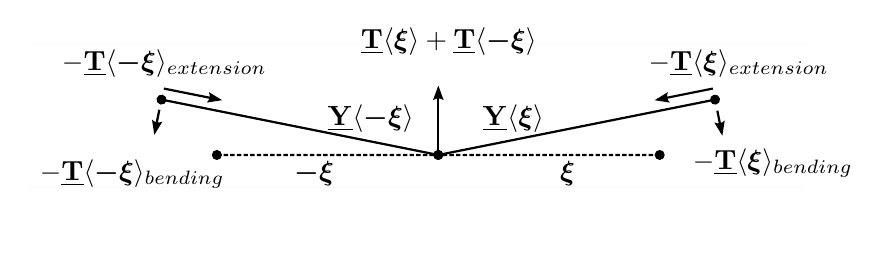
\begin{tikzpicture}[y=0.80pt, x=0.8pt,yscale=-1, inner sep=0pt, outer sep=0pt]
\begin{scope}[shift={(-16.10332,-55.70103)}]
  \begin{scope}[fill=black]
    \path[color=black,fill=black,line width=0.800pt] (101.0938,106.6875) --
      (103.0938,106.6875) -- (103.0938,105.6875) -- (101.0938,105.6875) --
      cycle(104.0938,106.6875) -- (106.0938,106.6875) -- (106.0938,105.6875) --
      (104.0938,105.6875) -- cycle(107.0938,106.6875) -- (109.0938,106.6875) --
      (109.0938,105.6875) -- (107.0938,105.6875) -- cycle(110.0938,106.6875) --
      (112.0938,106.6875) -- (112.0938,105.6875) -- (110.0938,105.6875) --
      cycle(113.0938,106.6875) -- (115.0938,106.6875) -- (115.0938,105.6875) --
      (113.0938,105.6875) -- cycle(116.0938,106.6875) -- (118.0938,106.6875) --
      (118.0938,105.6875) -- (116.0938,105.6875) -- cycle(119.0938,106.6875) --
      (121.0938,106.6875) -- (121.0938,105.6875) -- (119.0938,105.6875) --
      cycle(122.0938,106.6875) -- (124.0938,106.6875) -- (124.0938,105.6875) --
      (122.0938,105.6875) -- cycle(125.0938,106.6875) -- (127.0938,106.6875) --
      (127.0938,105.6875) -- (125.0938,105.6875) -- cycle(128.0938,106.6875) --
      (130.0938,106.6875) -- (130.0938,105.6875) -- (128.0938,105.6875) --
      cycle(131.0938,106.6875) -- (133.0938,106.6875) -- (133.0938,105.6875) --
      (131.0938,105.6875) -- cycle(134.0938,106.6875) -- (136.0938,106.6875) --
      (136.0938,105.6875) -- (134.0938,105.6875) -- cycle(137.0938,106.6875) --
      (139.0938,106.6875) -- (139.0938,105.6875) -- (137.0938,105.6875) --
      cycle(140.0938,106.6875) -- (142.0938,106.6875) -- (142.0938,105.6875) --
      (140.0938,105.6875) -- cycle(143.0938,106.6875) -- (145.0938,106.6875) --
      (145.0938,105.6875) -- (143.0938,105.6875) -- cycle(146.0938,106.6875) --
      (148.0938,106.6875) -- (148.0938,105.6875) -- (146.0938,105.6875) --
      cycle(149.0938,106.6875) -- (151.0938,106.6875) -- (151.0938,105.6875) --
      (149.0938,105.6875) -- cycle(152.0938,106.6875) -- (154.0938,106.6875) --
      (154.0938,105.6875) -- (152.0938,105.6875) -- cycle(155.0938,106.6875) --
      (157.0938,106.6875) -- (157.0938,105.6875) -- (155.0938,105.6875) --
      cycle(158.0938,106.6875) -- (160.0938,106.6875) -- (160.0938,105.6875) --
      (158.0938,105.6875) -- cycle(161.0938,106.6875) -- (163.0938,106.6875) --
      (163.0938,105.6875) -- (161.0938,105.6875) -- cycle(164.0938,106.6875) --
      (166.0938,106.6875) -- (166.0938,105.6875) -- (164.0938,105.6875) --
      cycle(167.0938,106.6875) -- (169.0938,106.6875) -- (169.0938,105.6875) --
      (167.0938,105.6875) -- cycle(170.0938,106.6875) -- (172.0938,106.6875) --
      (172.0938,105.6875) -- (170.0938,105.6875) -- cycle(173.0938,106.6875) --
      (175.0938,106.6875) -- (175.0938,105.6875) -- (173.0938,105.6875) --
      cycle(176.0938,106.6875) -- (178.0938,106.6875) -- (178.0938,105.6875) --
      (176.0938,105.6875) -- cycle(179.0938,106.6875) -- (181.0938,106.6875) --
      (181.0938,105.6875) -- (179.0938,105.6875) -- cycle(182.0938,106.6875) --
      (184.0938,106.6875) -- (184.0938,105.6875) -- (182.0938,105.6875) --
      cycle(185.0938,106.6875) -- (187.0938,106.6875) -- (187.0938,105.6875) --
      (185.0938,105.6875) -- cycle(188.0938,106.6875) -- (190.0938,106.6875) --
      (190.0938,105.6875) -- (188.0938,105.6875) -- cycle(191.0938,106.6875) --
      (193.0938,106.6875) -- (193.0938,105.6875) -- (191.0938,105.6875) --
      cycle(194.0938,106.6875) -- (196.0938,106.6875) -- (196.0938,105.6875) --
      (194.0938,105.6875) -- cycle(197.0938,106.6875) -- (199.0938,106.6875) --
      (199.0938,105.6875) -- (197.0938,105.6875) -- cycle(200.0938,106.6875) --
      (201.0938,106.6875) -- (202.0938,106.6875) -- (202.0938,105.6875) --
      (201.0938,105.6875) -- (200.0938,105.6875) -- cycle(203.0938,106.6875) --
      (205.0938,106.6875) -- (205.0938,105.6875) -- (203.0938,105.6875) --
      cycle(206.0938,106.6875) -- (208.0938,106.6875) -- (208.0938,105.6875) --
      (206.0938,105.6875) -- cycle(209.0938,106.6875) -- (211.0938,106.6875) --
      (211.0938,105.6875) -- (209.0938,105.6875) -- cycle(212.0938,106.6875) --
      (214.0938,106.6875) -- (214.0938,105.6875) -- (212.0938,105.6875) --
      cycle(215.0938,106.6875) -- (217.0938,106.6875) -- (217.0938,105.6875) --
      (215.0938,105.6875) -- cycle(218.0938,106.6875) -- (220.0938,106.6875) --
      (220.0938,105.6875) -- (218.0938,105.6875) -- cycle(221.0938,106.6875) --
      (223.0938,106.6875) -- (223.0938,105.6875) -- (221.0938,105.6875) --
      cycle(224.0938,106.6875) -- (226.0938,106.6875) -- (226.0938,105.6875) --
      (224.0938,105.6875) -- cycle(227.0938,106.6875) -- (229.0938,106.6875) --
      (229.0938,105.6875) -- (227.0938,105.6875) -- cycle(230.0938,106.6875) --
      (232.0938,106.6875) -- (232.0938,105.6875) -- (230.0938,105.6875) --
      cycle(233.0938,106.6875) -- (235.0938,106.6875) -- (235.0938,105.6875) --
      (233.0938,105.6875) -- cycle(236.0938,106.6875) -- (238.0938,106.6875) --
      (238.0938,105.6875) -- (236.0938,105.6875) -- cycle(239.0938,106.6875) --
      (241.0938,106.6875) -- (241.0938,105.6875) -- (239.0938,105.6875) --
      cycle(242.0938,106.6875) -- (244.0938,106.6875) -- (244.0938,105.6875) --
      (242.0938,105.6875) -- cycle(245.0938,106.6875) -- (247.0938,106.6875) --
      (247.0938,105.6875) -- (245.0938,105.6875) -- cycle(248.0938,106.6875) --
      (250.0938,106.6875) -- (250.0938,105.6875) -- (248.0938,105.6875) --
      cycle(251.0938,106.6875) -- (253.0938,106.6875) -- (253.0938,105.6875) --
      (251.0938,105.6875) -- cycle(254.0938,106.6875) -- (256.0938,106.6875) --
      (256.0938,105.6875) -- (254.0938,105.6875) -- cycle(257.0938,106.6875) --
      (259.0938,106.6875) -- (259.0938,105.6875) -- (257.0938,105.6875) --
      cycle(260.0938,106.6875) -- (262.0938,106.6875) -- (262.0938,105.6875) --
      (260.0938,105.6875) -- cycle(263.0938,106.6875) -- (265.0938,106.6875) --
      (265.0938,105.6875) -- (263.0938,105.6875) -- cycle(266.0938,106.6875) --
      (268.0938,106.6875) -- (268.0938,105.6875) -- (266.0938,105.6875) --
      cycle(269.0938,106.6875) -- (271.0938,106.6875) -- (271.0938,105.6875) --
      (269.0938,105.6875) -- cycle(272.0938,106.6875) -- (274.0938,106.6875) --
      (274.0938,105.6875) -- (272.0938,105.6875) -- cycle(275.0938,106.6875) --
      (277.0938,106.6875) -- (277.0938,105.6875) -- (275.0938,105.6875) --
      cycle(278.0938,106.6875) -- (280.0938,106.6875) -- (280.0938,105.6875) --
      (278.0938,105.6875) -- cycle(281.0938,106.6875) -- (283.0938,106.6875) --
      (283.0938,105.6875) -- (281.0938,105.6875) -- cycle(284.0938,106.6875) --
      (286.0938,106.6875) -- (286.0938,105.6875) -- (284.0938,105.6875) --
      cycle(287.0938,106.6875) -- (289.0938,106.6875) -- (289.0938,105.6875) --
      (287.0938,105.6875) -- cycle(290.0938,106.6875) -- (292.0938,106.6875) --
      (292.0938,105.6875) -- (290.0938,105.6875) -- cycle(293.0938,106.6875) --
      (295.0938,106.6875) -- (295.0938,105.6875) -- (293.0938,105.6875) --
      cycle(296.0938,106.6875) -- (298.0938,106.6875) -- (298.0938,105.6875) --
      (296.0938,105.6875) -- cycle(299.0938,106.6875) -- (301.0938,106.6875) --
      (301.0938,105.6875) -- (299.0938,105.6875) -- cycle;
    \path[draw=black,fill=black,even odd rule,line width=0.400pt]
      (103.0633,106.2010) .. controls (103.0633,107.3050) and (102.1673,108.2010) ..
      (101.0633,108.2010) .. controls (99.9593,108.2010) and (99.0633,107.3050) ..
      (99.0633,106.2010) .. controls (99.0633,105.0970) and (99.9593,104.2010) ..
      (101.0633,104.2010) .. controls (102.1673,104.2010) and (103.0633,105.0970) ..
      (103.0633,106.2010) -- cycle;
    \path[draw=black,fill=black,even odd rule,line width=0.400pt]
      (203.0633,106.2010) .. controls (203.0633,107.3050) and (202.1673,108.2010) ..
      (201.0633,108.2010) .. controls (199.9593,108.2010) and (199.0633,107.3050) ..
      (199.0633,106.2010) .. controls (199.0633,105.0970) and (199.9593,104.2010) ..
      (201.0633,104.2010) .. controls (202.1673,104.2010) and (203.0633,105.0970) ..
      (203.0633,106.2010) -- cycle;
    \path[draw=black,fill=black,even odd rule,line width=0.400pt]
      (303.0633,106.2010) .. controls (303.0633,107.3050) and (302.1673,108.2010) ..
      (301.0633,108.2010) .. controls (299.9593,108.2010) and (299.0633,107.3050) ..
      (299.0633,106.2010) .. controls (299.0633,105.0970) and (299.9593,104.2010) ..
      (301.0633,104.2010) .. controls (302.1673,104.2010) and (303.0633,105.0970) ..
      (303.0633,106.2010) -- cycle;
  \end{scope}
  \begin{scope}[fill=black]
    \path[color=black,fill=black,line width=0.800pt] (76.1875,80.7188) --
      (76.0000,81.6875) -- (201.0000,106.6875) -- (201.0937,106.7187) --
      (201.1874,106.6875) -- (326.1874,81.6875) -- (326.0000,80.7188) --
      (201.0938,105.6875) -- (76.1875,80.7188) -- cycle;
    \path[draw=black,fill=black,even odd rule,line width=0.400pt] (78.0253,81.5854)
      .. controls (77.8087,82.6680) and (76.7544,83.3709) .. (75.6719,83.1544) ..
      controls (74.5893,82.9378) and (73.8864,81.8835) .. (74.1029,80.8010) ..
      controls (74.3194,79.7184) and (75.3738,79.0155) .. (76.4563,79.2320) ..
      controls (77.5389,79.4485) and (78.2418,80.5029) .. (78.0253,81.5854) --
      cycle;
    \path[draw=black,fill=black,even odd rule,line width=0.400pt]
      (203.0633,106.2010) .. controls (203.0633,107.3050) and (202.1673,108.2010) ..
      (201.0633,108.2010) .. controls (199.9593,108.2010) and (199.0633,107.3050) ..
      (199.0633,106.2010) .. controls (199.0633,105.0970) and (199.9593,104.2010) ..
      (201.0633,104.2010) .. controls (202.1673,104.2010) and (203.0633,105.0970) ..
      (203.0633,106.2010) -- cycle;
    \path[draw=black,fill=black,even odd rule,line width=0.400pt] (328.0253,80.8166)
      .. controls (328.2418,81.8992) and (327.5389,82.9535) .. (326.4563,83.1700) ..
      controls (325.3738,83.3866) and (324.3194,82.6837) .. (324.1029,81.6011) ..
      controls (323.8864,80.5186) and (324.5893,79.4642) .. (325.6719,79.2477) ..
      controls (326.7544,79.0312) and (327.8087,79.7341) .. (328.0253,80.8166) --
      cycle;
  \end{scope}
  \begin{scope}[fill=black]
    \path[color=black,fill=black,line width=0.800pt] (200.5938,76.1875) --
      (200.5938,106.1875) -- (201.5938,106.1875) -- (201.5938,76.1875) --
      (200.5938,76.1875) -- cycle;
    \path[fill=black,line join=round,even odd rule,line width=0.500pt]
      (198.6831,81.4322) -- (201.0937,74.8767) -- (203.5043,81.4322) .. controls
      (202.0811,80.3849) and (200.1339,80.3909) .. (198.6831,81.4322) -- cycle;
  \end{scope}
  \path[fill=black] (178.797,148.02312) node[above right] (text6246) {};
  \path[fill=black] (256.10333,120.20103) node[above right] (text6273)
    {$\boldsymbol{\xi}$};
  \path[fill=black] (136.10332,120.20103) node[above right] (text6277)
    {$\boldsymbol{-\xi}$};
  \path[fill=black] (296.10333,71.201035) node[above right] (text6285)
    {$-\vstate{T}{}{\boldsymbol{\xi}}_{extension}$};
  \path[shift={(71.10332,65.91978)},draw=black,opacity=0.010,line join=miter,line
    cap=butt,line width=0.800pt] (-55.0000,54.7812) -- (295.0000,54.7812);
  \path[fill=black] (316.10333,116.20103) node[above right] (text4473)
    {$-\vstate{T}{}{\boldsymbol{\xi}}_{bending}$};
  \begin{scope}[shift={(0,-64.5)},shift={(0,0)}]
    \path[shift={(71.10332,65.91978)},draw=black,opacity=0.010,line join=miter,line
      cap=butt,line width=0.800pt] (-55.0000,54.7812) -- (295.0000,54.7812);
  \end{scope}
  \path[fill=black] (166.10332,61.201035) node[above right] (text4726)
    {$\vstate{T}{}{\boldsymbol{\xi}}+\vstate{T}{}{\boldsymbol{-\xi}}$};
  \begin{scope}[fill=black]
    \path[color=black,fill=black,line width=0.800pt] (74.5625,85.6875) --
      (72.5625,95.6875) -- (73.5625,95.9062) -- (75.5625,85.9062) --
      (74.5625,85.6875) -- cycle;
    \path[fill=black,line join=round,even odd rule,line width=0.500pt]
      (76.4671,91.1458) -- (72.8177,97.1013) -- (71.7395,90.2003) .. controls
      (72.9297,91.5064) and (74.8403,91.8824) .. (76.4671,91.1458) -- cycle;
  \end{scope}
  \begin{scope}[fill=black]
    \path[color=black,fill=black,line width=0.800pt] (77.1875,75.7188) --
      (77.0000,76.6875) -- (102.0000,81.6875) -- (102.1875,80.7188) --
      (77.1875,75.7188) -- cycle;
    \path[fill=black,line join=round,even odd rule,line width=0.500pt]
      (97.4484,77.8019) -- (103.4039,81.4513) -- (96.5029,82.5295) .. controls
      (97.8090,81.3393) and (98.1849,79.4287) .. (97.4484,77.8019) -- cycle;
  \end{scope}
  \begin{scope}[fill=black]
    \path[color=black,fill=black,line width=0.800pt] (327.5938,86.0938) --
      (326.6250,86.3125) -- (328.6250,96.3125) -- (329.5938,96.0938) --
      (327.5938,86.0938) -- cycle;
    \path[fill=black,line join=round,even odd rule,line width=0.500pt]
      (330.4506,90.5968) -- (329.3725,97.4978) -- (325.7230,91.5423) .. controls
      (327.3240,92.2902) and (329.2322,91.9024) .. (330.4507,90.5968) -- cycle;
  \end{scope}
  \begin{scope}[fill=black]
    \path[color=black,fill=black,line width=0.800pt] (325.0000,75.7188) --
      (300.0000,80.7188) -- (300.1875,81.6875) -- (325.1875,76.6875) --
      (325.0000,75.7188) -- cycle;
    \path[fill=black,line join=round,even odd rule,line width=0.500pt]
      (305.7075,82.5484) -- (298.8066,81.4702) -- (304.7620,77.8207) .. controls
      (304.0142,79.4217) and (304.4020,81.3299) .. (305.7075,82.5484) -- cycle;
  \end{scope}
  \path[fill=black] (21.103317,121.20103) node[above right] (text4217)
    {$-\vstate{T}{}{\boldsymbol{-\xi}}_{bending}$};
  \path[fill=black] (31.103317,71.201035) node[above right] (text4221)
    {$-\vstate{T}{}{\boldsymbol{-\xi}}_{extension}$};
  \path[fill=black] (221.10332,96.201035) node[above right] (text4282)
    {$\vstate{Y}{}{\boldsymbol{\xi}}$};
  \path[fill=black] (151.10332,96.201035) node[above right] (text4286)
    {$\vstate{Y}{}{\boldsymbol{-\xi}}$};
\end{scope}

\end{tikzpicture}


  \caption{The Hybrid Model Combines Bending and Extension Components}
  \label{fig:hybridmodel}
\end{figure}
%
As the two sides are pulled apart, the magnitude of the extension force in each bond increases, and the magnitude of the bending force decreases.  At the same time, the angle at which the extension force acts decreases, and the angle of action for the bending force increases.  For small amounts of bending and reasonable stretches, increased tension in the direction of the bond pair results in increase restorative force.

\section{Extension to arbitrary Poisson ratio}
\label{sec:arbitrary}
Although many materials have Poisson ratios of \(\nu\approx \sfrac{1}{3}\), it is nonetheless desirable to extend the model to materials with arbitrary Poisson ratios.  For isotropic, linearly elastic models of solid materials, Silling et al.\ extended the peridynamic material model to arbitrary material parameters in \cite{silling2007peridynamic} by decomposing the deformation into isotropic and deviatoric components.  In the absence of plastic deformation, we need only find the difference between the strain energy of a deformed bond-based plate and the strain energy of an elastic plate with Poisson's ratio \(\nu \neq \sfrac{1}{3}\).  The difference is a function of the isotropic strain in two dimensions, \(\theta_2\)
%
\begin{align}
    W' &= \frac{G\;h}{2}\left(\frac{3\nu-1}{1-\nu}\right)\theta_2^2 \notag \\
%    \theta_2 &= \frac{2}{m}\left(\underline{\omega x}\right)\bullet\underline{e} \notag \\
    \theta_2 &= \frac{2}{m}\int_A \omega(\boldsymbol{\xi})|\boldsymbol{\xi}|(|\vstate{Y}{}{\boldsymbol{\xi}}|-|\boldsymbol{\xi}|)\;dA_{\boldsymbol{\xi}} \notag \\
%    W_\text{total} &= \frac{G\;h}{2}\left(\frac{3\nu-1}{1-\nu}\right)\theta_2^2 + \frac{4\;G\;h}{m}\left(\underline{\omega e}\right)\bullet\underline{e}\notag
    W_\text{total} &= \frac{G\;h}{2}\left(\frac{3\nu-1}{1-\nu}\right)\theta_2^2 + \frac{4\;G\;h}{m}\int_A \omega(\boldsymbol{\xi})(|\vstate{Y}{}{\boldsymbol{\xi}}|-|\boldsymbol{\xi}|)^2\;dA_{\boldsymbol{\xi}}\notag
\end{align}
%
This is to be expected because the bond-based model was calibrated to the shear strain energy, leaving discrepancies proportional to the isotropic strain energy that fall to 0 as Poisson's ratio approaches \(\nu = \sfrac{1}{3}\).

This decomposition method inspires a similar approach to our plate model. To perform the same extension for the plate model in bending, we find the error in the 1-parameter strain energy for \(\nu \neq \sfrac{1}{3}\)
%
\begin{align}
    W'=&\frac{G h^3}{12(1-\nu)} \left(\kappa_1^2+\kappa_2^2+2\nu\kappa_1\kappa_2+2(1-\nu)\kappa_3^2 \right)\notag\\
    &-\frac{G h^3}{12(1-\frac{1}{3})} \left(\kappa_1^2+\kappa_2^2+\frac{2}{3}\nu\kappa_1\kappa_2+2(1-\frac{1}{3})\kappa_3^2 \right) \notag \\
    W'=&2G \frac{h^3}{12}\frac{3\nu-1}{1-\nu} \left(\frac{\kappa_1+\kappa_2}{2}\right)^2.\notag
\end{align}
%
The discrepancy in energy is proportional to the square of average curvature, \(\frac{\kappa_1+\kappa_2}{2} = \bar{\kappa}\), which we will also refer to as the isotropic curvature.  The isotropic curvature can be envisioned as the portion of the deformation that resembles a hemispherical bowl.  A complete decomposition of bending energy into isotropic and deviatoric components as performed by Fischer in \cite{fischer1992bending} produces a far more complex model and is unnecessary at this time.  For a single bond pair we can represent the curvature vector along the bond pair as 
%\marginpar{ maybe leave this out and go straight to the curvature vector?}
%
\begin{equation}
    \boldsymbol{\kappa} _{\hat{\boldsymbol{\xi}}} = \frac{\vstate{Y}{}{\boldsymbol{\xi}}+\vstate{Y}{}{\boldsymbol{-\xi}}}{|\boldsymbol{\xi}|^2}\notag
\end{equation}
%
%\begin{equation}
%    \kappa_{\hat{u}} = \frac{z(\mathbf{x}+\xi\hat{u})-2z(\mathbf{x})+z(\mathbf{x}-\xi\hat{u})}{\xi^2}\notag
%\end{equation}
%
For large rotations, we can define an average curvature vector \(\bar{\boldsymbol{\kappa}}\).
This leads us to model the average curvature as 
%
\begin{align}
    \bar{\boldsymbol{\kappa}} &= \frac{1}{m} \int_0^\delta \int_0^{2\pi}\omega(\xi)\frac{\vstate{Y}{}{\boldsymbol{\xi}}+\vstate{Y}{}{\boldsymbol{-\xi}}}{\xi^2} \xi {\rm d}\phi {\rm d}\xi ;\notag \\
    m &= \int_0^\delta \int_0^{2\pi}\omega(\xi)\xi {\rm d}\phi {\rm d}\xi. \notag
\end{align}
%
The weighting function \(\omega(\xi)\) performs the same function as in the previous section.
We can rewrite the energy discrepancy in terms of \(\bar{\boldsymbol{\kappa}}\).
%
\begin{equation}
    W'=2G\frac{h^3}{12}\frac{3\nu-1}{1-\nu}\bar{\boldsymbol{\kappa}}^2. \notag
\end{equation}
%
We can take the Fr\'{e}chet derivative (details in \ref{sec:frechet})\todo{Can you show the details in the Appendix?  Also, should the $dA$ be there?} to produce a correction force vector state
%
\begin{equation}
    \vstate{T'}{}{\boldsymbol{\xi}}=\frac{8G}{m}\frac{h^3}{12}\frac{3\nu-1}{1-\nu}\frac{\omega(\boldsymbol{\xi})}{\xi^2} \bar{\boldsymbol{\kappa}},
    \label{eq:pressureState}
\end{equation}
%
that is not directly dependent on the deformation of a single bond pair.  Instead, \cref{eq:pressureState} represents a bond-length dependent ``pressure'' applied to every pair of bonds extending from a node.  This ``pressure'' is proportional to the curvature vector at that node.
A weighting function \(\omega(\boldsymbol{\xi}) = |\boldsymbol{\xi}|\) can ensure that the integral expression for force at a point is convergent.  This extra term that is dependent on the bending of all the pairs around a material point means that the extension is not properly a \textit{bond-pair} model.  Instead, it would be more accurate to call it a \textit{bond-multiple} model, in which the bond forces and energies are functions of the relationship between a family of bonds.  In either the continuous or discrete cases, this model extension requires the additional step of evaluating the isotropic curvature at each point, but the increased complexity of the extended model captures in the local limit the behavior of a two-parameter elastic material plate.
%
\section{Numerical Simulation}
\subsection{Discretized Model}
Discretizing the bond-pair model is primarily matter of exchanging integrals for sums. 
%
\begin{align}
%\label{eq:discreteBeamw}
w(\boldsymbol{\xi}_i) &= \omega(\boldsymbol{\xi}_i)\alpha \left[1+\cos(\theta(\vstate{Y}{}{\boldsymbol{\xi}_i},\vstate{Y}{}{-\boldsymbol{\xi}_i})) \right] \notag \\
&\approx \omega(\boldsymbol{\xi}_i)\frac{\alpha}{2}\left(\frac{z(\mathbf{x}+\boldsymbol{\xi}_i)-2z(\mathbf{x})+z(\mathbf{x}-\boldsymbol{\xi}_i)}{\boldsymbol{\xi}_i}\right)^2 \notag
\end{align}
%
in which $\boldsymbol{\xi}_i$ is the $i^\textnormal{th}$ bond emanating from the point $\mathbf{x}$ to each of the $n$ points within distance $\delta$ of point $\mathbf{x}$.
%
\begin{align}
%    \label{eq:discretebeam}
    \alpha &= \frac{c\; (\Delta x)^2}{m} ;\; c= \frac{G}{(1-\nu)}\frac{h^3}{12};\; m=\sum_{i=1}^n \omega(\boldsymbol{\xi}_i)\boldsymbol{\xi}_i^2 \implies \nonumber \\
    W&=(\Delta x)^2 \sum_{i=1}^n \omega(\boldsymbol{\xi}_i)\frac{G}{2(1-\nu)}\frac{h^3}{12}\left(\frac{z(\mathbf{x}+\boldsymbol{\xi}_i)-2z(\mathbf{x})+z(\mathbf{x}-\boldsymbol{\xi}_i)}{|\boldsymbol{\xi}_i|}\right)^2 \notag
\end{align}
%
Discretization of the 1-parameter bending model results in the equation of motion
%
\begin{align}
    \label{eq:discreteEoM}
    \rho(\mathbf{x})\mathbf{\ddot{u}}(\mathbf{x}) = \mathbf{f}(\mathbf{x})&+\sum_i \omega(\boldsymbol{\xi}_i)\left\{\frac{\alpha(\mathbf{x})}{|\mathbf{p}_i |}\frac{\mathbf{p}_i}{|\mathbf{p}_i |}\times \left[ \frac{\mathbf{p}_i}{|\mathbf{p}_i |}\times \frac{\mathbf{q}_i}{|\mathbf{q}_i |}\right] \right.  \\
    & \left. -\frac{\alpha(\mathbf{x}+\boldsymbol{\xi}_i)}{|\mathbf{p}_i |}\frac{(-\mathbf{p}_i)}{|\mathbf{p}_i |}\times\left[\frac{(-\mathbf{p}_i)}{|\mathbf{p}_i |}\times \frac{\mathbf{r}_i}{|\mathbf{r}_i |} \right] \right\} \notag
\end{align}
with
\begin{align}
    \mathbf{p}_i &= \boldsymbol{\xi}_i+\mathbf{u}(\mathbf{x}+\boldsymbol{\xi}_i)-\mathbf{u}(\mathbf{x});\notag\\
    \mathbf{q}_i &= -\boldsymbol{\xi}_i+\mathbf{u}(\mathbf{x}-\boldsymbol{\xi}_i)-\mathbf{u}(\mathbf{x});\notag\\
    \mathbf{r}_i &= \boldsymbol{\xi}_i+\mathbf{u}(\mathbf{x}+2\boldsymbol{\xi}_i)-\mathbf{u}(\mathbf{x}+\boldsymbol{\xi}_i).\notag
\end{align}
%

Implementing the 2-parameter model requires finding the isotropic curvature at each point.
%
\begin{align*}
    \bar{\boldsymbol{\kappa}}(\mathbf{x}) &= \frac{1}{m} \sum_i \omega(\boldsymbol{\xi}_i)\frac{\mathbf{p}_i +\mathbf{q}_i }{\boldsymbol{\xi}_i^2};\notag \\
    m(\mathbf{x})  &= \sum_i \omega(\boldsymbol{\xi}_i); \notag \\
    \alpha^\text{iso}(\mathbf{x}) &= \frac{4G}{m}\frac{h^3}{12}\frac{3\nu-1}{1-\nu}(\Delta x)^2;\\
    f^\text{iso}(\mathbf{x}) &= \sum_j \left\{\left[\alpha^\text{iso}(\mathbf{x})\bar{\boldsymbol{\kappa}}(\mathbf{x})-\alpha^\text{iso}(\mathbf{x}+\boldsymbol{\xi}_j)\bar{\boldsymbol{\kappa}}(\mathbf{x}+\boldsymbol{\xi}_j) \right] \frac{\omega(\boldsymbol{\xi}_j)}{\boldsymbol{\xi}_j^2} \right\}
\end{align*}
%
Discretizing the bond-pair model as proposed above requires that nodes be evenly spaced, $\Delta x$, throughout the entire plate, otherwise the displacement \(z(\mathbf{x}-\boldsymbol{\xi}_i)\) is ill-defined.  For this reason, the discretization does not allow for areas of higher and lower ``resolution''. An extension to this discretization that would allow changing mesh resolution will require interpolation between the nodes.  
%
\subsection{Numerical Method}
\label{sec:NumMethod}
Model behavior is evaluated by implementing the discretized equation of motion.  The case of a square plate simply supported on all four sides is chosen for simplicity in both evaluation and comparison.  To implement the simply-supported condition, it was sufficient to constrain the vertical displacement of each node along the plate's four edges.  Boundary conditions such as clamped or guided supports and applied moments require careful treatment to ensure both meaningful results and ease of computation.  While applying displacement constraints is straightforward, the appropriate way to apply an angle constraint or moment to a peridynamic point or collection of points is less obvious.

Additionally, the simply-supported flat plate is a configuration with significant analytical treatment in the classical theories, making a better comparison case than configurations that may require comparison to finite element or other solution techniques.
%
\subsection{Results}
The simplest test case for this model is a linear-elastic square plate with Poisson's ratio \(\nu = \sfrac{1}{3}\) that is simply-supported on all 4 sides with a uniform transverse pressure load on the entire surface between the supports.  As expected from an energy-equivalent model, the slice along the plate's centerline shown in \cref{fig:plate_convergence_h} demonstrates good agreement between the static deflection predicted by the bond-pair model and that of classical linear elasticity as the horizon length shrinks.  This convergence only continues to a minimum horizon, below which the discretized equation of motion (\cref{eq:discreteEoM}) ceases to accurately approximate the continuous integral formulation (\cref{eq:PDstateEoM,eq:SillingForceNO}).  The minimum horizon size depends on the discretization; it appears that twice the node spacing is insufficient, and that three times the node spacing is sufficient.  The difference is evident in \cref{fig:plate_minimum_h}.
%
\begin{figure}[h]
  \centering
  \resizebox{0.55\linewidth}{!}{%% Creator: Matplotlib, PGF backend
%%
%% To include the figure in your LaTeX document, write
%%   \input{<filename>.pgf}
%%
%% Make sure the required packages are loaded in your preamble
%%   \usepackage{pgf}
%%
%% Figures using additional raster images can only be included by \input if
%% they are in the same directory as the main LaTeX file. For loading figures
%% from other directories you can use the `import` package
%%   \usepackage{import}
%% and then include the figures with
%%   \import{<path to file>}{<filename>.pgf}
%%
%% Matplotlib used the following preamble
%%
\begingroup%
\makeatletter%
\begin{pgfpicture}%
\pgfpathrectangle{\pgfpointorigin}{\pgfqpoint{6.000000in}{6.000000in}}%
\pgfusepath{use as bounding box}%
\begin{pgfscope}%
\pgfsetrectcap%
\pgfsetroundjoin%
\definecolor{currentfill}{rgb}{1.000000,1.000000,1.000000}%
\pgfsetfillcolor{currentfill}%
\pgfsetlinewidth{0.000000pt}%
\definecolor{currentstroke}{rgb}{1.000000,1.000000,1.000000}%
\pgfsetstrokecolor{currentstroke}%
\pgfsetdash{}{0pt}%
\pgfpathmoveto{\pgfqpoint{0.000000in}{0.000000in}}%
\pgfpathlineto{\pgfqpoint{6.000000in}{0.000000in}}%
\pgfpathlineto{\pgfqpoint{6.000000in}{6.000000in}}%
\pgfpathlineto{\pgfqpoint{0.000000in}{6.000000in}}%
\pgfpathclose%
\pgfusepath{fill}%
\end{pgfscope}%
\begin{pgfscope}%
\pgfsetrectcap%
\pgfsetroundjoin%
\definecolor{currentfill}{rgb}{1.000000,1.000000,1.000000}%
\pgfsetfillcolor{currentfill}%
\pgfsetlinewidth{0.000000pt}%
\definecolor{currentstroke}{rgb}{0.000000,0.000000,0.000000}%
\pgfsetstrokecolor{currentstroke}%
\pgfsetdash{}{0pt}%
\pgfpathmoveto{\pgfqpoint{0.750000in}{0.600000in}}%
\pgfpathlineto{\pgfqpoint{5.400000in}{0.600000in}}%
\pgfpathlineto{\pgfqpoint{5.400000in}{5.400000in}}%
\pgfpathlineto{\pgfqpoint{0.750000in}{5.400000in}}%
\pgfpathclose%
\pgfusepath{fill}%
\end{pgfscope}%
\begin{pgfscope}%
\pgfpathrectangle{\pgfqpoint{0.750000in}{0.600000in}}{\pgfqpoint{4.650000in}{4.800000in}} %
\pgfusepath{clip}%
\pgfsetrectcap%
\pgfsetroundjoin%
\pgfsetlinewidth{1.003750pt}%
\definecolor{currentstroke}{rgb}{0.000000,0.000000,1.000000}%
\pgfsetstrokecolor{currentstroke}%
\pgfsetdash{}{0pt}%
\pgfpathmoveto{\pgfqpoint{0.750000in}{5.400000in}}%
\pgfpathlineto{\pgfqpoint{0.796500in}{5.270617in}}%
\pgfpathlineto{\pgfqpoint{0.843000in}{5.141433in}}%
\pgfpathlineto{\pgfqpoint{0.889500in}{5.012646in}}%
\pgfpathlineto{\pgfqpoint{0.936000in}{4.884446in}}%
\pgfpathlineto{\pgfqpoint{0.982500in}{4.757015in}}%
\pgfpathlineto{\pgfqpoint{1.029000in}{4.630524in}}%
\pgfpathlineto{\pgfqpoint{1.075500in}{4.505137in}}%
\pgfpathlineto{\pgfqpoint{1.122000in}{4.381006in}}%
\pgfpathlineto{\pgfqpoint{1.168500in}{4.258277in}}%
\pgfpathlineto{\pgfqpoint{1.215000in}{4.137087in}}%
\pgfpathlineto{\pgfqpoint{1.261500in}{4.017568in}}%
\pgfpathlineto{\pgfqpoint{1.308000in}{3.899846in}}%
\pgfpathlineto{\pgfqpoint{1.354500in}{3.784039in}}%
\pgfpathlineto{\pgfqpoint{1.401000in}{3.670263in}}%
\pgfpathlineto{\pgfqpoint{1.447500in}{3.558623in}}%
\pgfpathlineto{\pgfqpoint{1.494000in}{3.449222in}}%
\pgfpathlineto{\pgfqpoint{1.540500in}{3.342155in}}%
\pgfpathlineto{\pgfqpoint{1.587000in}{3.237511in}}%
\pgfpathlineto{\pgfqpoint{1.633500in}{3.135374in}}%
\pgfpathlineto{\pgfqpoint{1.680000in}{3.035823in}}%
\pgfpathlineto{\pgfqpoint{1.726500in}{2.938933in}}%
\pgfpathlineto{\pgfqpoint{1.773000in}{2.844775in}}%
\pgfpathlineto{\pgfqpoint{1.819500in}{2.753417in}}%
\pgfpathlineto{\pgfqpoint{1.866000in}{2.664922in}}%
\pgfpathlineto{\pgfqpoint{1.912500in}{2.579349in}}%
\pgfpathlineto{\pgfqpoint{1.959000in}{2.496753in}}%
\pgfpathlineto{\pgfqpoint{2.005500in}{2.417186in}}%
\pgfpathlineto{\pgfqpoint{2.052000in}{2.340695in}}%
\pgfpathlineto{\pgfqpoint{2.098500in}{2.267325in}}%
\pgfpathlineto{\pgfqpoint{2.145000in}{2.197118in}}%
\pgfpathlineto{\pgfqpoint{2.191500in}{2.130112in}}%
\pgfpathlineto{\pgfqpoint{2.238000in}{2.066343in}}%
\pgfpathlineto{\pgfqpoint{2.284500in}{2.005847in}}%
\pgfpathlineto{\pgfqpoint{2.331000in}{1.948654in}}%
\pgfpathlineto{\pgfqpoint{2.377500in}{1.894795in}}%
\pgfpathlineto{\pgfqpoint{2.424000in}{1.844294in}}%
\pgfpathlineto{\pgfqpoint{2.470500in}{1.797178in}}%
\pgfpathlineto{\pgfqpoint{2.517000in}{1.753468in}}%
\pgfpathlineto{\pgfqpoint{2.563500in}{1.713182in}}%
\pgfpathlineto{\pgfqpoint{2.610000in}{1.676341in}}%
\pgfpathlineto{\pgfqpoint{2.656500in}{1.642959in}}%
\pgfpathlineto{\pgfqpoint{2.703000in}{1.613052in}}%
\pgfpathlineto{\pgfqpoint{2.749500in}{1.586634in}}%
\pgfpathlineto{\pgfqpoint{2.796000in}{1.563715in}}%
\pgfpathlineto{\pgfqpoint{2.842500in}{1.544306in}}%
\pgfpathlineto{\pgfqpoint{2.889000in}{1.528416in}}%
\pgfpathlineto{\pgfqpoint{2.935500in}{1.516051in}}%
\pgfpathlineto{\pgfqpoint{2.982000in}{1.507215in}}%
\pgfpathlineto{\pgfqpoint{3.028500in}{1.501913in}}%
\pgfpathlineto{\pgfqpoint{3.075000in}{1.500145in}}%
\pgfpathlineto{\pgfqpoint{3.121500in}{1.501913in}}%
\pgfpathlineto{\pgfqpoint{3.168000in}{1.507215in}}%
\pgfpathlineto{\pgfqpoint{3.214500in}{1.516051in}}%
\pgfpathlineto{\pgfqpoint{3.261000in}{1.528416in}}%
\pgfpathlineto{\pgfqpoint{3.307500in}{1.544306in}}%
\pgfpathlineto{\pgfqpoint{3.354000in}{1.563715in}}%
\pgfpathlineto{\pgfqpoint{3.400500in}{1.586634in}}%
\pgfpathlineto{\pgfqpoint{3.447000in}{1.613052in}}%
\pgfpathlineto{\pgfqpoint{3.493500in}{1.642959in}}%
\pgfpathlineto{\pgfqpoint{3.540000in}{1.676341in}}%
\pgfpathlineto{\pgfqpoint{3.586500in}{1.713182in}}%
\pgfpathlineto{\pgfqpoint{3.633000in}{1.753468in}}%
\pgfpathlineto{\pgfqpoint{3.679500in}{1.797178in}}%
\pgfpathlineto{\pgfqpoint{3.726000in}{1.844294in}}%
\pgfpathlineto{\pgfqpoint{3.772500in}{1.894795in}}%
\pgfpathlineto{\pgfqpoint{3.819000in}{1.948654in}}%
\pgfpathlineto{\pgfqpoint{3.865500in}{2.005847in}}%
\pgfpathlineto{\pgfqpoint{3.912000in}{2.066343in}}%
\pgfpathlineto{\pgfqpoint{3.958500in}{2.130112in}}%
\pgfpathlineto{\pgfqpoint{4.005000in}{2.197118in}}%
\pgfpathlineto{\pgfqpoint{4.051500in}{2.267325in}}%
\pgfpathlineto{\pgfqpoint{4.098000in}{2.340695in}}%
\pgfpathlineto{\pgfqpoint{4.144500in}{2.417186in}}%
\pgfpathlineto{\pgfqpoint{4.191000in}{2.496753in}}%
\pgfpathlineto{\pgfqpoint{4.237500in}{2.579349in}}%
\pgfpathlineto{\pgfqpoint{4.284000in}{2.664922in}}%
\pgfpathlineto{\pgfqpoint{4.330500in}{2.753417in}}%
\pgfpathlineto{\pgfqpoint{4.377000in}{2.844775in}}%
\pgfpathlineto{\pgfqpoint{4.423500in}{2.938933in}}%
\pgfpathlineto{\pgfqpoint{4.470000in}{3.035823in}}%
\pgfpathlineto{\pgfqpoint{4.516500in}{3.135374in}}%
\pgfpathlineto{\pgfqpoint{4.563000in}{3.237511in}}%
\pgfpathlineto{\pgfqpoint{4.609500in}{3.342155in}}%
\pgfpathlineto{\pgfqpoint{4.656000in}{3.449222in}}%
\pgfpathlineto{\pgfqpoint{4.702500in}{3.558623in}}%
\pgfpathlineto{\pgfqpoint{4.749000in}{3.670263in}}%
\pgfpathlineto{\pgfqpoint{4.795500in}{3.784039in}}%
\pgfpathlineto{\pgfqpoint{4.842000in}{3.899846in}}%
\pgfpathlineto{\pgfqpoint{4.888500in}{4.017568in}}%
\pgfpathlineto{\pgfqpoint{4.935000in}{4.137087in}}%
\pgfpathlineto{\pgfqpoint{4.981500in}{4.258277in}}%
\pgfpathlineto{\pgfqpoint{5.028000in}{4.381006in}}%
\pgfpathlineto{\pgfqpoint{5.074500in}{4.505137in}}%
\pgfpathlineto{\pgfqpoint{5.121000in}{4.630524in}}%
\pgfpathlineto{\pgfqpoint{5.167500in}{4.757015in}}%
\pgfpathlineto{\pgfqpoint{5.214000in}{4.884446in}}%
\pgfpathlineto{\pgfqpoint{5.260500in}{5.012646in}}%
\pgfpathlineto{\pgfqpoint{5.307000in}{5.141433in}}%
\pgfpathlineto{\pgfqpoint{5.353500in}{5.270617in}}%
\pgfpathlineto{\pgfqpoint{5.400000in}{5.400000in}}%
\pgfusepath{stroke}%
\end{pgfscope}%
\begin{pgfscope}%
\pgfpathrectangle{\pgfqpoint{0.750000in}{0.600000in}}{\pgfqpoint{4.650000in}{4.800000in}} %
\pgfusepath{clip}%
\pgfsetbuttcap%
\pgfsetmiterjoin%
\definecolor{currentfill}{rgb}{0.000000,0.500000,0.000000}%
\pgfsetfillcolor{currentfill}%
\pgfsetlinewidth{0.501875pt}%
\definecolor{currentstroke}{rgb}{0.000000,0.000000,0.000000}%
\pgfsetstrokecolor{currentstroke}%
\pgfsetdash{}{0pt}%
\pgfsys@defobject{currentmarker}{\pgfqpoint{-0.041667in}{-0.041667in}}{\pgfqpoint{0.041667in}{0.041667in}}{%
\pgfpathmoveto{\pgfqpoint{0.000000in}{0.041667in}}%
\pgfpathlineto{\pgfqpoint{-0.041667in}{-0.041667in}}%
\pgfpathlineto{\pgfqpoint{0.041667in}{-0.041667in}}%
\pgfpathclose%
\pgfusepath{stroke,fill}%
}%
\begin{pgfscope}%
\pgfsys@transformshift{0.750000in}{5.400000in}%
\pgfsys@useobject{currentmarker}{}%
\end{pgfscope}%
\begin{pgfscope}%
\pgfsys@transformshift{1.029000in}{4.310547in}%
\pgfsys@useobject{currentmarker}{}%
\end{pgfscope}%
\begin{pgfscope}%
\pgfsys@transformshift{1.308000in}{3.564782in}%
\pgfsys@useobject{currentmarker}{}%
\end{pgfscope}%
\begin{pgfscope}%
\pgfsys@transformshift{1.587000in}{2.898760in}%
\pgfsys@useobject{currentmarker}{}%
\end{pgfscope}%
\begin{pgfscope}%
\pgfsys@transformshift{1.866000in}{2.327648in}%
\pgfsys@useobject{currentmarker}{}%
\end{pgfscope}%
\begin{pgfscope}%
\pgfsys@transformshift{2.145000in}{1.860336in}%
\pgfsys@useobject{currentmarker}{}%
\end{pgfscope}%
\begin{pgfscope}%
\pgfsys@transformshift{2.424000in}{1.508532in}%
\pgfsys@useobject{currentmarker}{}%
\end{pgfscope}%
\begin{pgfscope}%
\pgfsys@transformshift{2.703000in}{1.277825in}%
\pgfsys@useobject{currentmarker}{}%
\end{pgfscope}%
\begin{pgfscope}%
\pgfsys@transformshift{2.982000in}{1.172269in}%
\pgfsys@useobject{currentmarker}{}%
\end{pgfscope}%
\begin{pgfscope}%
\pgfsys@transformshift{3.261000in}{1.193421in}%
\pgfsys@useobject{currentmarker}{}%
\end{pgfscope}%
\begin{pgfscope}%
\pgfsys@transformshift{3.540000in}{1.340945in}%
\pgfsys@useobject{currentmarker}{}%
\end{pgfscope}%
\begin{pgfscope}%
\pgfsys@transformshift{3.819000in}{1.612666in}%
\pgfsys@useobject{currentmarker}{}%
\end{pgfscope}%
\begin{pgfscope}%
\pgfsys@transformshift{4.098000in}{2.002922in}%
\pgfsys@useobject{currentmarker}{}%
\end{pgfscope}%
\begin{pgfscope}%
\pgfsys@transformshift{4.377000in}{2.507482in}%
\pgfsys@useobject{currentmarker}{}%
\end{pgfscope}%
\begin{pgfscope}%
\pgfsys@transformshift{4.656000in}{3.109556in}%
\pgfsys@useobject{currentmarker}{}%
\end{pgfscope}%
\begin{pgfscope}%
\pgfsys@transformshift{4.935000in}{3.805866in}%
\pgfsys@useobject{currentmarker}{}%
\end{pgfscope}%
\begin{pgfscope}%
\pgfsys@transformshift{5.214000in}{4.578216in}%
\pgfsys@useobject{currentmarker}{}%
\end{pgfscope}%
\end{pgfscope}%
\begin{pgfscope}%
\pgfpathrectangle{\pgfqpoint{0.750000in}{0.600000in}}{\pgfqpoint{4.650000in}{4.800000in}} %
\pgfusepath{clip}%
\pgfsetbuttcap%
\pgfsetmiterjoin%
\definecolor{currentfill}{rgb}{1.000000,0.000000,0.000000}%
\pgfsetfillcolor{currentfill}%
\pgfsetlinewidth{0.501875pt}%
\definecolor{currentstroke}{rgb}{0.000000,0.000000,0.000000}%
\pgfsetstrokecolor{currentstroke}%
\pgfsetdash{}{0pt}%
\pgfsys@defobject{currentmarker}{\pgfqpoint{-0.041667in}{-0.041667in}}{\pgfqpoint{0.041667in}{0.041667in}}{%
\pgfpathmoveto{\pgfqpoint{-0.041667in}{-0.041667in}}%
\pgfpathlineto{\pgfqpoint{0.041667in}{-0.041667in}}%
\pgfpathlineto{\pgfqpoint{0.041667in}{0.041667in}}%
\pgfpathlineto{\pgfqpoint{-0.041667in}{0.041667in}}%
\pgfpathclose%
\pgfusepath{stroke,fill}%
}%
\begin{pgfscope}%
\pgfsys@transformshift{0.843000in}{5.061173in}%
\pgfsys@useobject{currentmarker}{}%
\end{pgfscope}%
\begin{pgfscope}%
\pgfsys@transformshift{1.122000in}{4.266410in}%
\pgfsys@useobject{currentmarker}{}%
\end{pgfscope}%
\begin{pgfscope}%
\pgfsys@transformshift{1.401000in}{3.542014in}%
\pgfsys@useobject{currentmarker}{}%
\end{pgfscope}%
\begin{pgfscope}%
\pgfsys@transformshift{1.680000in}{2.900482in}%
\pgfsys@useobject{currentmarker}{}%
\end{pgfscope}%
\begin{pgfscope}%
\pgfsys@transformshift{1.959000in}{2.358675in}%
\pgfsys@useobject{currentmarker}{}%
\end{pgfscope}%
\begin{pgfscope}%
\pgfsys@transformshift{2.238000in}{1.927894in}%
\pgfsys@useobject{currentmarker}{}%
\end{pgfscope}%
\begin{pgfscope}%
\pgfsys@transformshift{2.517000in}{1.615664in}%
\pgfsys@useobject{currentmarker}{}%
\end{pgfscope}%
\begin{pgfscope}%
\pgfsys@transformshift{2.796000in}{1.426642in}%
\pgfsys@useobject{currentmarker}{}%
\end{pgfscope}%
\begin{pgfscope}%
\pgfsys@transformshift{3.075000in}{1.363366in}%
\pgfsys@useobject{currentmarker}{}%
\end{pgfscope}%
\begin{pgfscope}%
\pgfsys@transformshift{3.354000in}{1.426642in}%
\pgfsys@useobject{currentmarker}{}%
\end{pgfscope}%
\begin{pgfscope}%
\pgfsys@transformshift{3.633000in}{1.615663in}%
\pgfsys@useobject{currentmarker}{}%
\end{pgfscope}%
\begin{pgfscope}%
\pgfsys@transformshift{3.912000in}{1.927893in}%
\pgfsys@useobject{currentmarker}{}%
\end{pgfscope}%
\begin{pgfscope}%
\pgfsys@transformshift{4.191000in}{2.358673in}%
\pgfsys@useobject{currentmarker}{}%
\end{pgfscope}%
\begin{pgfscope}%
\pgfsys@transformshift{4.470000in}{2.900481in}%
\pgfsys@useobject{currentmarker}{}%
\end{pgfscope}%
\begin{pgfscope}%
\pgfsys@transformshift{4.749000in}{3.542013in}%
\pgfsys@useobject{currentmarker}{}%
\end{pgfscope}%
\begin{pgfscope}%
\pgfsys@transformshift{5.028000in}{4.266409in}%
\pgfsys@useobject{currentmarker}{}%
\end{pgfscope}%
\begin{pgfscope}%
\pgfsys@transformshift{5.307000in}{5.061173in}%
\pgfsys@useobject{currentmarker}{}%
\end{pgfscope}%
\end{pgfscope}%
\begin{pgfscope}%
\pgfpathrectangle{\pgfqpoint{0.750000in}{0.600000in}}{\pgfqpoint{4.650000in}{4.800000in}} %
\pgfusepath{clip}%
\pgfsetbuttcap%
\pgfsetroundjoin%
\definecolor{currentfill}{rgb}{0.000000,0.750000,0.750000}%
\pgfsetfillcolor{currentfill}%
\pgfsetlinewidth{0.501875pt}%
\definecolor{currentstroke}{rgb}{0.000000,0.000000,0.000000}%
\pgfsetstrokecolor{currentstroke}%
\pgfsetdash{}{0pt}%
\pgfsys@defobject{currentmarker}{\pgfqpoint{-0.041667in}{-0.041667in}}{\pgfqpoint{0.041667in}{0.041667in}}{%
\pgfpathmoveto{\pgfqpoint{0.000000in}{-0.041667in}}%
\pgfpathcurveto{\pgfqpoint{0.011050in}{-0.041667in}}{\pgfqpoint{0.021649in}{-0.037276in}}{\pgfqpoint{0.029463in}{-0.029463in}}%
\pgfpathcurveto{\pgfqpoint{0.037276in}{-0.021649in}}{\pgfqpoint{0.041667in}{-0.011050in}}{\pgfqpoint{0.041667in}{0.000000in}}%
\pgfpathcurveto{\pgfqpoint{0.041667in}{0.011050in}}{\pgfqpoint{0.037276in}{0.021649in}}{\pgfqpoint{0.029463in}{0.029463in}}%
\pgfpathcurveto{\pgfqpoint{0.021649in}{0.037276in}}{\pgfqpoint{0.011050in}{0.041667in}}{\pgfqpoint{0.000000in}{0.041667in}}%
\pgfpathcurveto{\pgfqpoint{-0.011050in}{0.041667in}}{\pgfqpoint{-0.021649in}{0.037276in}}{\pgfqpoint{-0.029463in}{0.029463in}}%
\pgfpathcurveto{\pgfqpoint{-0.037276in}{0.021649in}}{\pgfqpoint{-0.041667in}{0.011050in}}{\pgfqpoint{-0.041667in}{0.000000in}}%
\pgfpathcurveto{\pgfqpoint{-0.041667in}{-0.011050in}}{\pgfqpoint{-0.037276in}{-0.021649in}}{\pgfqpoint{-0.029463in}{-0.029463in}}%
\pgfpathcurveto{\pgfqpoint{-0.021649in}{-0.037276in}}{\pgfqpoint{-0.011050in}{-0.041667in}}{\pgfqpoint{0.000000in}{-0.041667in}}%
\pgfpathclose%
\pgfusepath{stroke,fill}%
}%
\begin{pgfscope}%
\pgfsys@transformshift{0.936000in}{4.859152in}%
\pgfsys@useobject{currentmarker}{}%
\end{pgfscope}%
\begin{pgfscope}%
\pgfsys@transformshift{1.215000in}{4.089881in}%
\pgfsys@useobject{currentmarker}{}%
\end{pgfscope}%
\begin{pgfscope}%
\pgfsys@transformshift{1.494000in}{3.386489in}%
\pgfsys@useobject{currentmarker}{}%
\end{pgfscope}%
\begin{pgfscope}%
\pgfsys@transformshift{1.773000in}{2.771560in}%
\pgfsys@useobject{currentmarker}{}%
\end{pgfscope}%
\begin{pgfscope}%
\pgfsys@transformshift{2.052000in}{2.260688in}%
\pgfsys@useobject{currentmarker}{}%
\end{pgfscope}%
\begin{pgfscope}%
\pgfsys@transformshift{2.331000in}{1.864451in}%
\pgfsys@useobject{currentmarker}{}%
\end{pgfscope}%
\begin{pgfscope}%
\pgfsys@transformshift{2.610000in}{1.589731in}%
\pgfsys@useobject{currentmarker}{}%
\end{pgfscope}%
\begin{pgfscope}%
\pgfsys@transformshift{2.889000in}{1.440670in}%
\pgfsys@useobject{currentmarker}{}%
\end{pgfscope}%
\begin{pgfscope}%
\pgfsys@transformshift{3.168000in}{1.419313in}%
\pgfsys@useobject{currentmarker}{}%
\end{pgfscope}%
\begin{pgfscope}%
\pgfsys@transformshift{3.447000in}{1.525941in}%
\pgfsys@useobject{currentmarker}{}%
\end{pgfscope}%
\begin{pgfscope}%
\pgfsys@transformshift{3.726000in}{1.759121in}%
\pgfsys@useobject{currentmarker}{}%
\end{pgfscope}%
\begin{pgfscope}%
\pgfsys@transformshift{4.005000in}{2.115465in}%
\pgfsys@useobject{currentmarker}{}%
\end{pgfscope}%
\begin{pgfscope}%
\pgfsys@transformshift{4.284000in}{2.589095in}%
\pgfsys@useobject{currentmarker}{}%
\end{pgfscope}%
\begin{pgfscope}%
\pgfsys@transformshift{4.563000in}{3.170791in}%
\pgfsys@useobject{currentmarker}{}%
\end{pgfscope}%
\begin{pgfscope}%
\pgfsys@transformshift{4.842000in}{3.846810in}%
\pgfsys@useobject{currentmarker}{}%
\end{pgfscope}%
\begin{pgfscope}%
\pgfsys@transformshift{5.121000in}{4.597132in}%
\pgfsys@useobject{currentmarker}{}%
\end{pgfscope}%
\begin{pgfscope}%
\pgfsys@transformshift{5.400000in}{5.400000in}%
\pgfsys@useobject{currentmarker}{}%
\end{pgfscope}%
\end{pgfscope}%
\begin{pgfscope}%
\pgfpathrectangle{\pgfqpoint{0.750000in}{0.600000in}}{\pgfqpoint{4.650000in}{4.800000in}} %
\pgfusepath{clip}%
\pgfsetbuttcap%
\pgfsetroundjoin%
\pgfsetlinewidth{0.501875pt}%
\definecolor{currentstroke}{rgb}{0.000000,0.000000,0.000000}%
\pgfsetstrokecolor{currentstroke}%
\pgfsetdash{{1.000000pt}{3.000000pt}}{0.000000pt}%
\pgfpathmoveto{\pgfqpoint{0.750000in}{0.600000in}}%
\pgfpathlineto{\pgfqpoint{0.750000in}{5.400000in}}%
\pgfusepath{stroke}%
\end{pgfscope}%
\begin{pgfscope}%
\pgfsetbuttcap%
\pgfsetroundjoin%
\definecolor{currentfill}{rgb}{0.000000,0.000000,0.000000}%
\pgfsetfillcolor{currentfill}%
\pgfsetlinewidth{0.501875pt}%
\definecolor{currentstroke}{rgb}{0.000000,0.000000,0.000000}%
\pgfsetstrokecolor{currentstroke}%
\pgfsetdash{}{0pt}%
\pgfsys@defobject{currentmarker}{\pgfqpoint{0.000000in}{0.000000in}}{\pgfqpoint{0.000000in}{0.055556in}}{%
\pgfpathmoveto{\pgfqpoint{0.000000in}{0.000000in}}%
\pgfpathlineto{\pgfqpoint{0.000000in}{0.055556in}}%
\pgfusepath{stroke,fill}%
}%
\begin{pgfscope}%
\pgfsys@transformshift{0.750000in}{0.600000in}%
\pgfsys@useobject{currentmarker}{}%
\end{pgfscope}%
\end{pgfscope}%
\begin{pgfscope}%
\pgfsetbuttcap%
\pgfsetroundjoin%
\definecolor{currentfill}{rgb}{0.000000,0.000000,0.000000}%
\pgfsetfillcolor{currentfill}%
\pgfsetlinewidth{0.501875pt}%
\definecolor{currentstroke}{rgb}{0.000000,0.000000,0.000000}%
\pgfsetstrokecolor{currentstroke}%
\pgfsetdash{}{0pt}%
\pgfsys@defobject{currentmarker}{\pgfqpoint{0.000000in}{-0.055556in}}{\pgfqpoint{0.000000in}{0.000000in}}{%
\pgfpathmoveto{\pgfqpoint{0.000000in}{0.000000in}}%
\pgfpathlineto{\pgfqpoint{0.000000in}{-0.055556in}}%
\pgfusepath{stroke,fill}%
}%
\begin{pgfscope}%
\pgfsys@transformshift{0.750000in}{5.400000in}%
\pgfsys@useobject{currentmarker}{}%
\end{pgfscope}%
\end{pgfscope}%
\begin{pgfscope}%
\pgftext[left,bottom,x=0.604940in,y=0.437037in,rotate=0.000000]{{\rmfamily\fontsize{12.000000}{14.400000}\selectfont \(\displaystyle 0.00\)}}
%
\end{pgfscope}%
\begin{pgfscope}%
\pgfpathrectangle{\pgfqpoint{0.750000in}{0.600000in}}{\pgfqpoint{4.650000in}{4.800000in}} %
\pgfusepath{clip}%
\pgfsetbuttcap%
\pgfsetroundjoin%
\pgfsetlinewidth{0.501875pt}%
\definecolor{currentstroke}{rgb}{0.000000,0.000000,0.000000}%
\pgfsetstrokecolor{currentstroke}%
\pgfsetdash{{1.000000pt}{3.000000pt}}{0.000000pt}%
\pgfpathmoveto{\pgfqpoint{1.912500in}{0.600000in}}%
\pgfpathlineto{\pgfqpoint{1.912500in}{5.400000in}}%
\pgfusepath{stroke}%
\end{pgfscope}%
\begin{pgfscope}%
\pgfsetbuttcap%
\pgfsetroundjoin%
\definecolor{currentfill}{rgb}{0.000000,0.000000,0.000000}%
\pgfsetfillcolor{currentfill}%
\pgfsetlinewidth{0.501875pt}%
\definecolor{currentstroke}{rgb}{0.000000,0.000000,0.000000}%
\pgfsetstrokecolor{currentstroke}%
\pgfsetdash{}{0pt}%
\pgfsys@defobject{currentmarker}{\pgfqpoint{0.000000in}{0.000000in}}{\pgfqpoint{0.000000in}{0.055556in}}{%
\pgfpathmoveto{\pgfqpoint{0.000000in}{0.000000in}}%
\pgfpathlineto{\pgfqpoint{0.000000in}{0.055556in}}%
\pgfusepath{stroke,fill}%
}%
\begin{pgfscope}%
\pgfsys@transformshift{1.912500in}{0.600000in}%
\pgfsys@useobject{currentmarker}{}%
\end{pgfscope}%
\end{pgfscope}%
\begin{pgfscope}%
\pgfsetbuttcap%
\pgfsetroundjoin%
\definecolor{currentfill}{rgb}{0.000000,0.000000,0.000000}%
\pgfsetfillcolor{currentfill}%
\pgfsetlinewidth{0.501875pt}%
\definecolor{currentstroke}{rgb}{0.000000,0.000000,0.000000}%
\pgfsetstrokecolor{currentstroke}%
\pgfsetdash{}{0pt}%
\pgfsys@defobject{currentmarker}{\pgfqpoint{0.000000in}{-0.055556in}}{\pgfqpoint{0.000000in}{0.000000in}}{%
\pgfpathmoveto{\pgfqpoint{0.000000in}{0.000000in}}%
\pgfpathlineto{\pgfqpoint{0.000000in}{-0.055556in}}%
\pgfusepath{stroke,fill}%
}%
\begin{pgfscope}%
\pgfsys@transformshift{1.912500in}{5.400000in}%
\pgfsys@useobject{currentmarker}{}%
\end{pgfscope}%
\end{pgfscope}%
\begin{pgfscope}%
\pgftext[left,bottom,x=1.767440in,y=0.437037in,rotate=0.000000]{{\rmfamily\fontsize{12.000000}{14.400000}\selectfont \(\displaystyle 0.25\)}}
%
\end{pgfscope}%
\begin{pgfscope}%
\pgfpathrectangle{\pgfqpoint{0.750000in}{0.600000in}}{\pgfqpoint{4.650000in}{4.800000in}} %
\pgfusepath{clip}%
\pgfsetbuttcap%
\pgfsetroundjoin%
\pgfsetlinewidth{0.501875pt}%
\definecolor{currentstroke}{rgb}{0.000000,0.000000,0.000000}%
\pgfsetstrokecolor{currentstroke}%
\pgfsetdash{{1.000000pt}{3.000000pt}}{0.000000pt}%
\pgfpathmoveto{\pgfqpoint{3.075000in}{0.600000in}}%
\pgfpathlineto{\pgfqpoint{3.075000in}{5.400000in}}%
\pgfusepath{stroke}%
\end{pgfscope}%
\begin{pgfscope}%
\pgfsetbuttcap%
\pgfsetroundjoin%
\definecolor{currentfill}{rgb}{0.000000,0.000000,0.000000}%
\pgfsetfillcolor{currentfill}%
\pgfsetlinewidth{0.501875pt}%
\definecolor{currentstroke}{rgb}{0.000000,0.000000,0.000000}%
\pgfsetstrokecolor{currentstroke}%
\pgfsetdash{}{0pt}%
\pgfsys@defobject{currentmarker}{\pgfqpoint{0.000000in}{0.000000in}}{\pgfqpoint{0.000000in}{0.055556in}}{%
\pgfpathmoveto{\pgfqpoint{0.000000in}{0.000000in}}%
\pgfpathlineto{\pgfqpoint{0.000000in}{0.055556in}}%
\pgfusepath{stroke,fill}%
}%
\begin{pgfscope}%
\pgfsys@transformshift{3.075000in}{0.600000in}%
\pgfsys@useobject{currentmarker}{}%
\end{pgfscope}%
\end{pgfscope}%
\begin{pgfscope}%
\pgfsetbuttcap%
\pgfsetroundjoin%
\definecolor{currentfill}{rgb}{0.000000,0.000000,0.000000}%
\pgfsetfillcolor{currentfill}%
\pgfsetlinewidth{0.501875pt}%
\definecolor{currentstroke}{rgb}{0.000000,0.000000,0.000000}%
\pgfsetstrokecolor{currentstroke}%
\pgfsetdash{}{0pt}%
\pgfsys@defobject{currentmarker}{\pgfqpoint{0.000000in}{-0.055556in}}{\pgfqpoint{0.000000in}{0.000000in}}{%
\pgfpathmoveto{\pgfqpoint{0.000000in}{0.000000in}}%
\pgfpathlineto{\pgfqpoint{0.000000in}{-0.055556in}}%
\pgfusepath{stroke,fill}%
}%
\begin{pgfscope}%
\pgfsys@transformshift{3.075000in}{5.400000in}%
\pgfsys@useobject{currentmarker}{}%
\end{pgfscope}%
\end{pgfscope}%
\begin{pgfscope}%
\pgftext[left,bottom,x=2.929940in,y=0.437037in,rotate=0.000000]{{\rmfamily\fontsize{12.000000}{14.400000}\selectfont \(\displaystyle 0.50\)}}
%
\end{pgfscope}%
\begin{pgfscope}%
\pgfpathrectangle{\pgfqpoint{0.750000in}{0.600000in}}{\pgfqpoint{4.650000in}{4.800000in}} %
\pgfusepath{clip}%
\pgfsetbuttcap%
\pgfsetroundjoin%
\pgfsetlinewidth{0.501875pt}%
\definecolor{currentstroke}{rgb}{0.000000,0.000000,0.000000}%
\pgfsetstrokecolor{currentstroke}%
\pgfsetdash{{1.000000pt}{3.000000pt}}{0.000000pt}%
\pgfpathmoveto{\pgfqpoint{4.237500in}{0.600000in}}%
\pgfpathlineto{\pgfqpoint{4.237500in}{5.400000in}}%
\pgfusepath{stroke}%
\end{pgfscope}%
\begin{pgfscope}%
\pgfsetbuttcap%
\pgfsetroundjoin%
\definecolor{currentfill}{rgb}{0.000000,0.000000,0.000000}%
\pgfsetfillcolor{currentfill}%
\pgfsetlinewidth{0.501875pt}%
\definecolor{currentstroke}{rgb}{0.000000,0.000000,0.000000}%
\pgfsetstrokecolor{currentstroke}%
\pgfsetdash{}{0pt}%
\pgfsys@defobject{currentmarker}{\pgfqpoint{0.000000in}{0.000000in}}{\pgfqpoint{0.000000in}{0.055556in}}{%
\pgfpathmoveto{\pgfqpoint{0.000000in}{0.000000in}}%
\pgfpathlineto{\pgfqpoint{0.000000in}{0.055556in}}%
\pgfusepath{stroke,fill}%
}%
\begin{pgfscope}%
\pgfsys@transformshift{4.237500in}{0.600000in}%
\pgfsys@useobject{currentmarker}{}%
\end{pgfscope}%
\end{pgfscope}%
\begin{pgfscope}%
\pgfsetbuttcap%
\pgfsetroundjoin%
\definecolor{currentfill}{rgb}{0.000000,0.000000,0.000000}%
\pgfsetfillcolor{currentfill}%
\pgfsetlinewidth{0.501875pt}%
\definecolor{currentstroke}{rgb}{0.000000,0.000000,0.000000}%
\pgfsetstrokecolor{currentstroke}%
\pgfsetdash{}{0pt}%
\pgfsys@defobject{currentmarker}{\pgfqpoint{0.000000in}{-0.055556in}}{\pgfqpoint{0.000000in}{0.000000in}}{%
\pgfpathmoveto{\pgfqpoint{0.000000in}{0.000000in}}%
\pgfpathlineto{\pgfqpoint{0.000000in}{-0.055556in}}%
\pgfusepath{stroke,fill}%
}%
\begin{pgfscope}%
\pgfsys@transformshift{4.237500in}{5.400000in}%
\pgfsys@useobject{currentmarker}{}%
\end{pgfscope}%
\end{pgfscope}%
\begin{pgfscope}%
\pgftext[left,bottom,x=4.092440in,y=0.437037in,rotate=0.000000]{{\rmfamily\fontsize{12.000000}{14.400000}\selectfont \(\displaystyle 0.75\)}}
%
\end{pgfscope}%
\begin{pgfscope}%
\pgfpathrectangle{\pgfqpoint{0.750000in}{0.600000in}}{\pgfqpoint{4.650000in}{4.800000in}} %
\pgfusepath{clip}%
\pgfsetbuttcap%
\pgfsetroundjoin%
\pgfsetlinewidth{0.501875pt}%
\definecolor{currentstroke}{rgb}{0.000000,0.000000,0.000000}%
\pgfsetstrokecolor{currentstroke}%
\pgfsetdash{{1.000000pt}{3.000000pt}}{0.000000pt}%
\pgfpathmoveto{\pgfqpoint{5.400000in}{0.600000in}}%
\pgfpathlineto{\pgfqpoint{5.400000in}{5.400000in}}%
\pgfusepath{stroke}%
\end{pgfscope}%
\begin{pgfscope}%
\pgfsetbuttcap%
\pgfsetroundjoin%
\definecolor{currentfill}{rgb}{0.000000,0.000000,0.000000}%
\pgfsetfillcolor{currentfill}%
\pgfsetlinewidth{0.501875pt}%
\definecolor{currentstroke}{rgb}{0.000000,0.000000,0.000000}%
\pgfsetstrokecolor{currentstroke}%
\pgfsetdash{}{0pt}%
\pgfsys@defobject{currentmarker}{\pgfqpoint{0.000000in}{0.000000in}}{\pgfqpoint{0.000000in}{0.055556in}}{%
\pgfpathmoveto{\pgfqpoint{0.000000in}{0.000000in}}%
\pgfpathlineto{\pgfqpoint{0.000000in}{0.055556in}}%
\pgfusepath{stroke,fill}%
}%
\begin{pgfscope}%
\pgfsys@transformshift{5.400000in}{0.600000in}%
\pgfsys@useobject{currentmarker}{}%
\end{pgfscope}%
\end{pgfscope}%
\begin{pgfscope}%
\pgfsetbuttcap%
\pgfsetroundjoin%
\definecolor{currentfill}{rgb}{0.000000,0.000000,0.000000}%
\pgfsetfillcolor{currentfill}%
\pgfsetlinewidth{0.501875pt}%
\definecolor{currentstroke}{rgb}{0.000000,0.000000,0.000000}%
\pgfsetstrokecolor{currentstroke}%
\pgfsetdash{}{0pt}%
\pgfsys@defobject{currentmarker}{\pgfqpoint{0.000000in}{-0.055556in}}{\pgfqpoint{0.000000in}{0.000000in}}{%
\pgfpathmoveto{\pgfqpoint{0.000000in}{0.000000in}}%
\pgfpathlineto{\pgfqpoint{0.000000in}{-0.055556in}}%
\pgfusepath{stroke,fill}%
}%
\begin{pgfscope}%
\pgfsys@transformshift{5.400000in}{5.400000in}%
\pgfsys@useobject{currentmarker}{}%
\end{pgfscope}%
\end{pgfscope}%
\begin{pgfscope}%
\pgftext[left,bottom,x=5.254940in,y=0.437037in,rotate=0.000000]{{\rmfamily\fontsize{12.000000}{14.400000}\selectfont \(\displaystyle 1.00\)}}
%
\end{pgfscope}%
\begin{pgfscope}%
\pgftext[left,bottom,x=1.923189in,y=0.219445in,rotate=0.000000]{{\rmfamily\fontsize{12.000000}{14.400000}\selectfont Distance Along Plate Centerline}}
%
\end{pgfscope}%
\begin{pgfscope}%
\pgfpathrectangle{\pgfqpoint{0.750000in}{0.600000in}}{\pgfqpoint{4.650000in}{4.800000in}} %
\pgfusepath{clip}%
\pgfsetbuttcap%
\pgfsetroundjoin%
\pgfsetlinewidth{0.501875pt}%
\definecolor{currentstroke}{rgb}{0.000000,0.000000,0.000000}%
\pgfsetstrokecolor{currentstroke}%
\pgfsetdash{{1.000000pt}{3.000000pt}}{0.000000pt}%
\pgfpathmoveto{\pgfqpoint{0.750000in}{5.400000in}}%
\pgfpathlineto{\pgfqpoint{5.400000in}{5.400000in}}%
\pgfusepath{stroke}%
\end{pgfscope}%
\begin{pgfscope}%
\pgfsetbuttcap%
\pgfsetroundjoin%
\definecolor{currentfill}{rgb}{0.000000,0.000000,0.000000}%
\pgfsetfillcolor{currentfill}%
\pgfsetlinewidth{0.501875pt}%
\definecolor{currentstroke}{rgb}{0.000000,0.000000,0.000000}%
\pgfsetstrokecolor{currentstroke}%
\pgfsetdash{}{0pt}%
\pgfsys@defobject{currentmarker}{\pgfqpoint{0.000000in}{0.000000in}}{\pgfqpoint{0.055556in}{0.000000in}}{%
\pgfpathmoveto{\pgfqpoint{0.000000in}{0.000000in}}%
\pgfpathlineto{\pgfqpoint{0.055556in}{0.000000in}}%
\pgfusepath{stroke,fill}%
}%
\begin{pgfscope}%
\pgfsys@transformshift{0.750000in}{5.400000in}%
\pgfsys@useobject{currentmarker}{}%
\end{pgfscope}%
\end{pgfscope}%
\begin{pgfscope}%
\pgfsetbuttcap%
\pgfsetroundjoin%
\definecolor{currentfill}{rgb}{0.000000,0.000000,0.000000}%
\pgfsetfillcolor{currentfill}%
\pgfsetlinewidth{0.501875pt}%
\definecolor{currentstroke}{rgb}{0.000000,0.000000,0.000000}%
\pgfsetstrokecolor{currentstroke}%
\pgfsetdash{}{0pt}%
\pgfsys@defobject{currentmarker}{\pgfqpoint{-0.055556in}{0.000000in}}{\pgfqpoint{0.000000in}{0.000000in}}{%
\pgfpathmoveto{\pgfqpoint{0.000000in}{0.000000in}}%
\pgfpathlineto{\pgfqpoint{-0.055556in}{0.000000in}}%
\pgfusepath{stroke,fill}%
}%
\begin{pgfscope}%
\pgfsys@transformshift{5.400000in}{5.400000in}%
\pgfsys@useobject{currentmarker}{}%
\end{pgfscope}%
\end{pgfscope}%
\begin{pgfscope}%
\pgftext[left,bottom,x=0.612848in,y=5.346296in,rotate=0.000000]{{\rmfamily\fontsize{12.000000}{14.400000}\selectfont \(\displaystyle 0\)}}
%
\end{pgfscope}%
\begin{pgfscope}%
\pgfpathrectangle{\pgfqpoint{0.750000in}{0.600000in}}{\pgfqpoint{4.650000in}{4.800000in}} %
\pgfusepath{clip}%
\pgfsetbuttcap%
\pgfsetroundjoin%
\pgfsetlinewidth{0.501875pt}%
\definecolor{currentstroke}{rgb}{0.000000,0.000000,0.000000}%
\pgfsetstrokecolor{currentstroke}%
\pgfsetdash{{1.000000pt}{3.000000pt}}{0.000000pt}%
\pgfpathmoveto{\pgfqpoint{0.750000in}{4.440000in}}%
\pgfpathlineto{\pgfqpoint{5.400000in}{4.440000in}}%
\pgfusepath{stroke}%
\end{pgfscope}%
\begin{pgfscope}%
\pgfsetbuttcap%
\pgfsetroundjoin%
\definecolor{currentfill}{rgb}{0.000000,0.000000,0.000000}%
\pgfsetfillcolor{currentfill}%
\pgfsetlinewidth{0.501875pt}%
\definecolor{currentstroke}{rgb}{0.000000,0.000000,0.000000}%
\pgfsetstrokecolor{currentstroke}%
\pgfsetdash{}{0pt}%
\pgfsys@defobject{currentmarker}{\pgfqpoint{0.000000in}{0.000000in}}{\pgfqpoint{0.055556in}{0.000000in}}{%
\pgfpathmoveto{\pgfqpoint{0.000000in}{0.000000in}}%
\pgfpathlineto{\pgfqpoint{0.055556in}{0.000000in}}%
\pgfusepath{stroke,fill}%
}%
\begin{pgfscope}%
\pgfsys@transformshift{0.750000in}{4.440000in}%
\pgfsys@useobject{currentmarker}{}%
\end{pgfscope}%
\end{pgfscope}%
\begin{pgfscope}%
\pgfsetbuttcap%
\pgfsetroundjoin%
\definecolor{currentfill}{rgb}{0.000000,0.000000,0.000000}%
\pgfsetfillcolor{currentfill}%
\pgfsetlinewidth{0.501875pt}%
\definecolor{currentstroke}{rgb}{0.000000,0.000000,0.000000}%
\pgfsetstrokecolor{currentstroke}%
\pgfsetdash{}{0pt}%
\pgfsys@defobject{currentmarker}{\pgfqpoint{-0.055556in}{0.000000in}}{\pgfqpoint{0.000000in}{0.000000in}}{%
\pgfpathmoveto{\pgfqpoint{0.000000in}{0.000000in}}%
\pgfpathlineto{\pgfqpoint{-0.055556in}{0.000000in}}%
\pgfusepath{stroke,fill}%
}%
\begin{pgfscope}%
\pgfsys@transformshift{5.400000in}{4.440000in}%
\pgfsys@useobject{currentmarker}{}%
\end{pgfscope}%
\end{pgfscope}%
\begin{pgfscope}%
\pgftext[left,bottom,x=0.483218in,y=4.379352in,rotate=0.000000]{{\rmfamily\fontsize{12.000000}{14.400000}\selectfont \(\displaystyle -1\)}}
%
\end{pgfscope}%
\begin{pgfscope}%
\pgfpathrectangle{\pgfqpoint{0.750000in}{0.600000in}}{\pgfqpoint{4.650000in}{4.800000in}} %
\pgfusepath{clip}%
\pgfsetbuttcap%
\pgfsetroundjoin%
\pgfsetlinewidth{0.501875pt}%
\definecolor{currentstroke}{rgb}{0.000000,0.000000,0.000000}%
\pgfsetstrokecolor{currentstroke}%
\pgfsetdash{{1.000000pt}{3.000000pt}}{0.000000pt}%
\pgfpathmoveto{\pgfqpoint{0.750000in}{3.480000in}}%
\pgfpathlineto{\pgfqpoint{5.400000in}{3.480000in}}%
\pgfusepath{stroke}%
\end{pgfscope}%
\begin{pgfscope}%
\pgfsetbuttcap%
\pgfsetroundjoin%
\definecolor{currentfill}{rgb}{0.000000,0.000000,0.000000}%
\pgfsetfillcolor{currentfill}%
\pgfsetlinewidth{0.501875pt}%
\definecolor{currentstroke}{rgb}{0.000000,0.000000,0.000000}%
\pgfsetstrokecolor{currentstroke}%
\pgfsetdash{}{0pt}%
\pgfsys@defobject{currentmarker}{\pgfqpoint{0.000000in}{0.000000in}}{\pgfqpoint{0.055556in}{0.000000in}}{%
\pgfpathmoveto{\pgfqpoint{0.000000in}{0.000000in}}%
\pgfpathlineto{\pgfqpoint{0.055556in}{0.000000in}}%
\pgfusepath{stroke,fill}%
}%
\begin{pgfscope}%
\pgfsys@transformshift{0.750000in}{3.480000in}%
\pgfsys@useobject{currentmarker}{}%
\end{pgfscope}%
\end{pgfscope}%
\begin{pgfscope}%
\pgfsetbuttcap%
\pgfsetroundjoin%
\definecolor{currentfill}{rgb}{0.000000,0.000000,0.000000}%
\pgfsetfillcolor{currentfill}%
\pgfsetlinewidth{0.501875pt}%
\definecolor{currentstroke}{rgb}{0.000000,0.000000,0.000000}%
\pgfsetstrokecolor{currentstroke}%
\pgfsetdash{}{0pt}%
\pgfsys@defobject{currentmarker}{\pgfqpoint{-0.055556in}{0.000000in}}{\pgfqpoint{0.000000in}{0.000000in}}{%
\pgfpathmoveto{\pgfqpoint{0.000000in}{0.000000in}}%
\pgfpathlineto{\pgfqpoint{-0.055556in}{0.000000in}}%
\pgfusepath{stroke,fill}%
}%
\begin{pgfscope}%
\pgfsys@transformshift{5.400000in}{3.480000in}%
\pgfsys@useobject{currentmarker}{}%
\end{pgfscope}%
\end{pgfscope}%
\begin{pgfscope}%
\pgftext[left,bottom,x=0.483218in,y=3.419352in,rotate=0.000000]{{\rmfamily\fontsize{12.000000}{14.400000}\selectfont \(\displaystyle -2\)}}
%
\end{pgfscope}%
\begin{pgfscope}%
\pgfpathrectangle{\pgfqpoint{0.750000in}{0.600000in}}{\pgfqpoint{4.650000in}{4.800000in}} %
\pgfusepath{clip}%
\pgfsetbuttcap%
\pgfsetroundjoin%
\pgfsetlinewidth{0.501875pt}%
\definecolor{currentstroke}{rgb}{0.000000,0.000000,0.000000}%
\pgfsetstrokecolor{currentstroke}%
\pgfsetdash{{1.000000pt}{3.000000pt}}{0.000000pt}%
\pgfpathmoveto{\pgfqpoint{0.750000in}{2.520000in}}%
\pgfpathlineto{\pgfqpoint{5.400000in}{2.520000in}}%
\pgfusepath{stroke}%
\end{pgfscope}%
\begin{pgfscope}%
\pgfsetbuttcap%
\pgfsetroundjoin%
\definecolor{currentfill}{rgb}{0.000000,0.000000,0.000000}%
\pgfsetfillcolor{currentfill}%
\pgfsetlinewidth{0.501875pt}%
\definecolor{currentstroke}{rgb}{0.000000,0.000000,0.000000}%
\pgfsetstrokecolor{currentstroke}%
\pgfsetdash{}{0pt}%
\pgfsys@defobject{currentmarker}{\pgfqpoint{0.000000in}{0.000000in}}{\pgfqpoint{0.055556in}{0.000000in}}{%
\pgfpathmoveto{\pgfqpoint{0.000000in}{0.000000in}}%
\pgfpathlineto{\pgfqpoint{0.055556in}{0.000000in}}%
\pgfusepath{stroke,fill}%
}%
\begin{pgfscope}%
\pgfsys@transformshift{0.750000in}{2.520000in}%
\pgfsys@useobject{currentmarker}{}%
\end{pgfscope}%
\end{pgfscope}%
\begin{pgfscope}%
\pgfsetbuttcap%
\pgfsetroundjoin%
\definecolor{currentfill}{rgb}{0.000000,0.000000,0.000000}%
\pgfsetfillcolor{currentfill}%
\pgfsetlinewidth{0.501875pt}%
\definecolor{currentstroke}{rgb}{0.000000,0.000000,0.000000}%
\pgfsetstrokecolor{currentstroke}%
\pgfsetdash{}{0pt}%
\pgfsys@defobject{currentmarker}{\pgfqpoint{-0.055556in}{0.000000in}}{\pgfqpoint{0.000000in}{0.000000in}}{%
\pgfpathmoveto{\pgfqpoint{0.000000in}{0.000000in}}%
\pgfpathlineto{\pgfqpoint{-0.055556in}{0.000000in}}%
\pgfusepath{stroke,fill}%
}%
\begin{pgfscope}%
\pgfsys@transformshift{5.400000in}{2.520000in}%
\pgfsys@useobject{currentmarker}{}%
\end{pgfscope}%
\end{pgfscope}%
\begin{pgfscope}%
\pgftext[left,bottom,x=0.483218in,y=2.459352in,rotate=0.000000]{{\rmfamily\fontsize{12.000000}{14.400000}\selectfont \(\displaystyle -3\)}}
%
\end{pgfscope}%
\begin{pgfscope}%
\pgfpathrectangle{\pgfqpoint{0.750000in}{0.600000in}}{\pgfqpoint{4.650000in}{4.800000in}} %
\pgfusepath{clip}%
\pgfsetbuttcap%
\pgfsetroundjoin%
\pgfsetlinewidth{0.501875pt}%
\definecolor{currentstroke}{rgb}{0.000000,0.000000,0.000000}%
\pgfsetstrokecolor{currentstroke}%
\pgfsetdash{{1.000000pt}{3.000000pt}}{0.000000pt}%
\pgfpathmoveto{\pgfqpoint{0.750000in}{1.560000in}}%
\pgfpathlineto{\pgfqpoint{5.400000in}{1.560000in}}%
\pgfusepath{stroke}%
\end{pgfscope}%
\begin{pgfscope}%
\pgfsetbuttcap%
\pgfsetroundjoin%
\definecolor{currentfill}{rgb}{0.000000,0.000000,0.000000}%
\pgfsetfillcolor{currentfill}%
\pgfsetlinewidth{0.501875pt}%
\definecolor{currentstroke}{rgb}{0.000000,0.000000,0.000000}%
\pgfsetstrokecolor{currentstroke}%
\pgfsetdash{}{0pt}%
\pgfsys@defobject{currentmarker}{\pgfqpoint{0.000000in}{0.000000in}}{\pgfqpoint{0.055556in}{0.000000in}}{%
\pgfpathmoveto{\pgfqpoint{0.000000in}{0.000000in}}%
\pgfpathlineto{\pgfqpoint{0.055556in}{0.000000in}}%
\pgfusepath{stroke,fill}%
}%
\begin{pgfscope}%
\pgfsys@transformshift{0.750000in}{1.560000in}%
\pgfsys@useobject{currentmarker}{}%
\end{pgfscope}%
\end{pgfscope}%
\begin{pgfscope}%
\pgfsetbuttcap%
\pgfsetroundjoin%
\definecolor{currentfill}{rgb}{0.000000,0.000000,0.000000}%
\pgfsetfillcolor{currentfill}%
\pgfsetlinewidth{0.501875pt}%
\definecolor{currentstroke}{rgb}{0.000000,0.000000,0.000000}%
\pgfsetstrokecolor{currentstroke}%
\pgfsetdash{}{0pt}%
\pgfsys@defobject{currentmarker}{\pgfqpoint{-0.055556in}{0.000000in}}{\pgfqpoint{0.000000in}{0.000000in}}{%
\pgfpathmoveto{\pgfqpoint{0.000000in}{0.000000in}}%
\pgfpathlineto{\pgfqpoint{-0.055556in}{0.000000in}}%
\pgfusepath{stroke,fill}%
}%
\begin{pgfscope}%
\pgfsys@transformshift{5.400000in}{1.560000in}%
\pgfsys@useobject{currentmarker}{}%
\end{pgfscope}%
\end{pgfscope}%
\begin{pgfscope}%
\pgftext[left,bottom,x=0.483218in,y=1.499352in,rotate=0.000000]{{\rmfamily\fontsize{12.000000}{14.400000}\selectfont \(\displaystyle -4\)}}
%
\end{pgfscope}%
\begin{pgfscope}%
\pgfpathrectangle{\pgfqpoint{0.750000in}{0.600000in}}{\pgfqpoint{4.650000in}{4.800000in}} %
\pgfusepath{clip}%
\pgfsetbuttcap%
\pgfsetroundjoin%
\pgfsetlinewidth{0.501875pt}%
\definecolor{currentstroke}{rgb}{0.000000,0.000000,0.000000}%
\pgfsetstrokecolor{currentstroke}%
\pgfsetdash{{1.000000pt}{3.000000pt}}{0.000000pt}%
\pgfpathmoveto{\pgfqpoint{0.750000in}{0.600000in}}%
\pgfpathlineto{\pgfqpoint{5.400000in}{0.600000in}}%
\pgfusepath{stroke}%
\end{pgfscope}%
\begin{pgfscope}%
\pgfsetbuttcap%
\pgfsetroundjoin%
\definecolor{currentfill}{rgb}{0.000000,0.000000,0.000000}%
\pgfsetfillcolor{currentfill}%
\pgfsetlinewidth{0.501875pt}%
\definecolor{currentstroke}{rgb}{0.000000,0.000000,0.000000}%
\pgfsetstrokecolor{currentstroke}%
\pgfsetdash{}{0pt}%
\pgfsys@defobject{currentmarker}{\pgfqpoint{0.000000in}{0.000000in}}{\pgfqpoint{0.055556in}{0.000000in}}{%
\pgfpathmoveto{\pgfqpoint{0.000000in}{0.000000in}}%
\pgfpathlineto{\pgfqpoint{0.055556in}{0.000000in}}%
\pgfusepath{stroke,fill}%
}%
\begin{pgfscope}%
\pgfsys@transformshift{0.750000in}{0.600000in}%
\pgfsys@useobject{currentmarker}{}%
\end{pgfscope}%
\end{pgfscope}%
\begin{pgfscope}%
\pgfsetbuttcap%
\pgfsetroundjoin%
\definecolor{currentfill}{rgb}{0.000000,0.000000,0.000000}%
\pgfsetfillcolor{currentfill}%
\pgfsetlinewidth{0.501875pt}%
\definecolor{currentstroke}{rgb}{0.000000,0.000000,0.000000}%
\pgfsetstrokecolor{currentstroke}%
\pgfsetdash{}{0pt}%
\pgfsys@defobject{currentmarker}{\pgfqpoint{-0.055556in}{0.000000in}}{\pgfqpoint{0.000000in}{0.000000in}}{%
\pgfpathmoveto{\pgfqpoint{0.000000in}{0.000000in}}%
\pgfpathlineto{\pgfqpoint{-0.055556in}{0.000000in}}%
\pgfusepath{stroke,fill}%
}%
\begin{pgfscope}%
\pgfsys@transformshift{5.400000in}{0.600000in}%
\pgfsys@useobject{currentmarker}{}%
\end{pgfscope}%
\end{pgfscope}%
\begin{pgfscope}%
\pgftext[left,bottom,x=0.483218in,y=0.539352in,rotate=0.000000]{{\rmfamily\fontsize{12.000000}{14.400000}\selectfont \(\displaystyle -5\)}}
%
\end{pgfscope}%
\begin{pgfscope}%
\pgftext[left,bottom,x=0.413774in,y=1.761606in,rotate=90.000000]{{\rmfamily\fontsize{12.000000}{14.400000}\selectfont Deflection under Uniform Pressure}}
%
\end{pgfscope}%
\begin{pgfscope}%
\pgftext[left,bottom,x=0.750000in,y=5.427778in,rotate=0.000000]{{\rmfamily\fontsize{12.000000}{14.400000}\selectfont \(\displaystyle \times10^{-5}\)}}
%
\end{pgfscope}%
\begin{pgfscope}%
\pgfsetrectcap%
\pgfsetroundjoin%
\pgfsetlinewidth{1.003750pt}%
\definecolor{currentstroke}{rgb}{0.000000,0.000000,0.000000}%
\pgfsetstrokecolor{currentstroke}%
\pgfsetdash{}{0pt}%
\pgfpathmoveto{\pgfqpoint{0.750000in}{5.400000in}}%
\pgfpathlineto{\pgfqpoint{5.400000in}{5.400000in}}%
\pgfusepath{stroke}%
\end{pgfscope}%
\begin{pgfscope}%
\pgfsetrectcap%
\pgfsetroundjoin%
\pgfsetlinewidth{1.003750pt}%
\definecolor{currentstroke}{rgb}{0.000000,0.000000,0.000000}%
\pgfsetstrokecolor{currentstroke}%
\pgfsetdash{}{0pt}%
\pgfpathmoveto{\pgfqpoint{5.400000in}{0.600000in}}%
\pgfpathlineto{\pgfqpoint{5.400000in}{5.400000in}}%
\pgfusepath{stroke}%
\end{pgfscope}%
\begin{pgfscope}%
\pgfsetrectcap%
\pgfsetroundjoin%
\pgfsetlinewidth{1.003750pt}%
\definecolor{currentstroke}{rgb}{0.000000,0.000000,0.000000}%
\pgfsetstrokecolor{currentstroke}%
\pgfsetdash{}{0pt}%
\pgfpathmoveto{\pgfqpoint{0.750000in}{0.600000in}}%
\pgfpathlineto{\pgfqpoint{5.400000in}{0.600000in}}%
\pgfusepath{stroke}%
\end{pgfscope}%
\begin{pgfscope}%
\pgfsetrectcap%
\pgfsetroundjoin%
\pgfsetlinewidth{1.003750pt}%
\definecolor{currentstroke}{rgb}{0.000000,0.000000,0.000000}%
\pgfsetstrokecolor{currentstroke}%
\pgfsetdash{}{0pt}%
\pgfpathmoveto{\pgfqpoint{0.750000in}{0.600000in}}%
\pgfpathlineto{\pgfqpoint{0.750000in}{5.400000in}}%
\pgfusepath{stroke}%
\end{pgfscope}%
\begin{pgfscope}%
\pgftext[left,bottom,x=1.817076in,y=5.430556in,rotate=0.000000]{{\rmfamily\fontsize{14.400000}{17.280000}\selectfont Simply Supported Plate Slice}}
%
\end{pgfscope}%
\begin{pgfscope}%
\pgfsetrectcap%
\pgfsetroundjoin%
\definecolor{currentfill}{rgb}{1.000000,1.000000,1.000000}%
\pgfsetfillcolor{currentfill}%
\pgfsetlinewidth{1.003750pt}%
\definecolor{currentstroke}{rgb}{0.000000,0.000000,0.000000}%
\pgfsetstrokecolor{currentstroke}%
\pgfsetdash{}{0pt}%
\pgfpathmoveto{\pgfqpoint{1.928413in}{4.224445in}}%
\pgfpathlineto{\pgfqpoint{4.221587in}{4.224445in}}%
\pgfpathlineto{\pgfqpoint{4.221587in}{5.400000in}}%
\pgfpathlineto{\pgfqpoint{1.928413in}{5.400000in}}%
\pgfpathlineto{\pgfqpoint{1.928413in}{4.224445in}}%
\pgfpathclose%
\pgfusepath{stroke,fill}%
\end{pgfscope}%
\begin{pgfscope}%
\pgfsetrectcap%
\pgfsetroundjoin%
\pgfsetlinewidth{1.003750pt}%
\definecolor{currentstroke}{rgb}{0.000000,0.000000,1.000000}%
\pgfsetstrokecolor{currentstroke}%
\pgfsetdash{}{0pt}%
\pgfpathmoveto{\pgfqpoint{2.068413in}{5.250000in}}%
\pgfpathlineto{\pgfqpoint{2.348413in}{5.250000in}}%
\pgfusepath{stroke}%
\end{pgfscope}%
\begin{pgfscope}%
\pgftext[left,bottom,x=2.568413in,y=5.141111in,rotate=0.000000]{{\rmfamily\fontsize{14.400000}{17.280000}\selectfont Analytical}}
%
\end{pgfscope}%
\begin{pgfscope}%
\pgfsetbuttcap%
\pgfsetmiterjoin%
\definecolor{currentfill}{rgb}{0.000000,0.500000,0.000000}%
\pgfsetfillcolor{currentfill}%
\pgfsetlinewidth{0.501875pt}%
\definecolor{currentstroke}{rgb}{0.000000,0.000000,0.000000}%
\pgfsetstrokecolor{currentstroke}%
\pgfsetdash{}{0pt}%
\pgfsys@defobject{currentmarker}{\pgfqpoint{-0.041667in}{-0.041667in}}{\pgfqpoint{0.041667in}{0.041667in}}{%
\pgfpathmoveto{\pgfqpoint{0.000000in}{0.041667in}}%
\pgfpathlineto{\pgfqpoint{-0.041667in}{-0.041667in}}%
\pgfpathlineto{\pgfqpoint{0.041667in}{-0.041667in}}%
\pgfpathclose%
\pgfusepath{stroke,fill}%
}%
\begin{pgfscope}%
\pgfsys@transformshift{2.068413in}{4.971111in}%
\pgfsys@useobject{currentmarker}{}%
\end{pgfscope}%
\begin{pgfscope}%
\pgfsys@transformshift{2.348413in}{4.971111in}%
\pgfsys@useobject{currentmarker}{}%
\end{pgfscope}%
\end{pgfscope}%
\begin{pgfscope}%
\pgftext[left,bottom,x=2.568413in,y=4.862223in,rotate=0.000000]{{\rmfamily\fontsize{14.400000}{17.280000}\selectfont 100 nodes, h=0.15}}
%
\end{pgfscope}%
\begin{pgfscope}%
\pgfsetbuttcap%
\pgfsetmiterjoin%
\definecolor{currentfill}{rgb}{1.000000,0.000000,0.000000}%
\pgfsetfillcolor{currentfill}%
\pgfsetlinewidth{0.501875pt}%
\definecolor{currentstroke}{rgb}{0.000000,0.000000,0.000000}%
\pgfsetstrokecolor{currentstroke}%
\pgfsetdash{}{0pt}%
\pgfsys@defobject{currentmarker}{\pgfqpoint{-0.041667in}{-0.041667in}}{\pgfqpoint{0.041667in}{0.041667in}}{%
\pgfpathmoveto{\pgfqpoint{-0.041667in}{-0.041667in}}%
\pgfpathlineto{\pgfqpoint{0.041667in}{-0.041667in}}%
\pgfpathlineto{\pgfqpoint{0.041667in}{0.041667in}}%
\pgfpathlineto{\pgfqpoint{-0.041667in}{0.041667in}}%
\pgfpathclose%
\pgfusepath{stroke,fill}%
}%
\begin{pgfscope}%
\pgfsys@transformshift{2.068413in}{4.692223in}%
\pgfsys@useobject{currentmarker}{}%
\end{pgfscope}%
\begin{pgfscope}%
\pgfsys@transformshift{2.348413in}{4.692223in}%
\pgfsys@useobject{currentmarker}{}%
\end{pgfscope}%
\end{pgfscope}%
\begin{pgfscope}%
\pgftext[left,bottom,x=2.568413in,y=4.583334in,rotate=0.000000]{{\rmfamily\fontsize{14.400000}{17.280000}\selectfont 100 nodes, h=0.10}}
%
\end{pgfscope}%
\begin{pgfscope}%
\pgfsetbuttcap%
\pgfsetroundjoin%
\definecolor{currentfill}{rgb}{0.000000,0.750000,0.750000}%
\pgfsetfillcolor{currentfill}%
\pgfsetlinewidth{0.501875pt}%
\definecolor{currentstroke}{rgb}{0.000000,0.000000,0.000000}%
\pgfsetstrokecolor{currentstroke}%
\pgfsetdash{}{0pt}%
\pgfsys@defobject{currentmarker}{\pgfqpoint{-0.041667in}{-0.041667in}}{\pgfqpoint{0.041667in}{0.041667in}}{%
\pgfpathmoveto{\pgfqpoint{0.000000in}{-0.041667in}}%
\pgfpathcurveto{\pgfqpoint{0.011050in}{-0.041667in}}{\pgfqpoint{0.021649in}{-0.037276in}}{\pgfqpoint{0.029463in}{-0.029463in}}%
\pgfpathcurveto{\pgfqpoint{0.037276in}{-0.021649in}}{\pgfqpoint{0.041667in}{-0.011050in}}{\pgfqpoint{0.041667in}{0.000000in}}%
\pgfpathcurveto{\pgfqpoint{0.041667in}{0.011050in}}{\pgfqpoint{0.037276in}{0.021649in}}{\pgfqpoint{0.029463in}{0.029463in}}%
\pgfpathcurveto{\pgfqpoint{0.021649in}{0.037276in}}{\pgfqpoint{0.011050in}{0.041667in}}{\pgfqpoint{0.000000in}{0.041667in}}%
\pgfpathcurveto{\pgfqpoint{-0.011050in}{0.041667in}}{\pgfqpoint{-0.021649in}{0.037276in}}{\pgfqpoint{-0.029463in}{0.029463in}}%
\pgfpathcurveto{\pgfqpoint{-0.037276in}{0.021649in}}{\pgfqpoint{-0.041667in}{0.011050in}}{\pgfqpoint{-0.041667in}{0.000000in}}%
\pgfpathcurveto{\pgfqpoint{-0.041667in}{-0.011050in}}{\pgfqpoint{-0.037276in}{-0.021649in}}{\pgfqpoint{-0.029463in}{-0.029463in}}%
\pgfpathcurveto{\pgfqpoint{-0.021649in}{-0.037276in}}{\pgfqpoint{-0.011050in}{-0.041667in}}{\pgfqpoint{0.000000in}{-0.041667in}}%
\pgfpathclose%
\pgfusepath{stroke,fill}%
}%
\begin{pgfscope}%
\pgfsys@transformshift{2.068413in}{4.413334in}%
\pgfsys@useobject{currentmarker}{}%
\end{pgfscope}%
\begin{pgfscope}%
\pgfsys@transformshift{2.348413in}{4.413334in}%
\pgfsys@useobject{currentmarker}{}%
\end{pgfscope}%
\end{pgfscope}%
\begin{pgfscope}%
\pgftext[left,bottom,x=2.568413in,y=4.304445in,rotate=0.000000]{{\rmfamily\fontsize{14.400000}{17.280000}\selectfont 100 nodes, h=0.05}}
%
\end{pgfscope}%
\end{pgfpicture}%
\makeatother%
\endgroup%
}
  \caption{The Bond-Pair Model Converges on Accurate Plate Deflection with Smaller Horizons}
  \label{fig:plate_convergence_h}
\end{figure}
%
\begin{figure}[h]
  \centering
  \resizebox{0.55\linewidth}{!}{%% Creator: Matplotlib, PGF backend
%%
%% To include the figure in your LaTeX document, write
%%   \input{<filename>.pgf}
%%
%% Make sure the required packages are loaded in your preamble
%%   \usepackage{pgf}
%%
%% Figures using additional raster images can only be included by \input if
%% they are in the same directory as the main LaTeX file. For loading figures
%% from other directories you can use the `import` package
%%   \usepackage{import}
%% and then include the figures with
%%   \import{<path to file>}{<filename>.pgf}
%%
%% Matplotlib used the following preamble
%%
\begingroup%
\makeatletter%
\begin{pgfpicture}%
\pgfpathrectangle{\pgfpointorigin}{\pgfqpoint{6.000000in}{6.000000in}}%
\pgfusepath{use as bounding box}%
\begin{pgfscope}%
\pgfsetrectcap%
\pgfsetroundjoin%
\definecolor{currentfill}{rgb}{1.000000,1.000000,1.000000}%
\pgfsetfillcolor{currentfill}%
\pgfsetlinewidth{0.000000pt}%
\definecolor{currentstroke}{rgb}{1.000000,1.000000,1.000000}%
\pgfsetstrokecolor{currentstroke}%
\pgfsetdash{}{0pt}%
\pgfpathmoveto{\pgfqpoint{0.000000in}{0.000000in}}%
\pgfpathlineto{\pgfqpoint{6.000000in}{0.000000in}}%
\pgfpathlineto{\pgfqpoint{6.000000in}{6.000000in}}%
\pgfpathlineto{\pgfqpoint{0.000000in}{6.000000in}}%
\pgfpathclose%
\pgfusepath{fill}%
\end{pgfscope}%
\begin{pgfscope}%
\pgfsetrectcap%
\pgfsetroundjoin%
\definecolor{currentfill}{rgb}{1.000000,1.000000,1.000000}%
\pgfsetfillcolor{currentfill}%
\pgfsetlinewidth{0.000000pt}%
\definecolor{currentstroke}{rgb}{0.000000,0.000000,0.000000}%
\pgfsetstrokecolor{currentstroke}%
\pgfsetdash{}{0pt}%
\pgfpathmoveto{\pgfqpoint{0.750000in}{0.600000in}}%
\pgfpathlineto{\pgfqpoint{5.400000in}{0.600000in}}%
\pgfpathlineto{\pgfqpoint{5.400000in}{5.400000in}}%
\pgfpathlineto{\pgfqpoint{0.750000in}{5.400000in}}%
\pgfpathclose%
\pgfusepath{fill}%
\end{pgfscope}%
\begin{pgfscope}%
\pgfpathrectangle{\pgfqpoint{0.750000in}{0.600000in}}{\pgfqpoint{4.650000in}{4.800000in}} %
\pgfusepath{clip}%
\pgfsetrectcap%
\pgfsetroundjoin%
\pgfsetlinewidth{1.003750pt}%
\definecolor{currentstroke}{rgb}{0.000000,0.000000,1.000000}%
\pgfsetstrokecolor{currentstroke}%
\pgfsetdash{}{0pt}%
\pgfpathmoveto{\pgfqpoint{0.750000in}{5.400000in}}%
\pgfpathlineto{\pgfqpoint{0.959250in}{4.820624in}}%
\pgfpathlineto{\pgfqpoint{1.075500in}{4.505137in}}%
\pgfpathlineto{\pgfqpoint{1.168500in}{4.258277in}}%
\pgfpathlineto{\pgfqpoint{1.261500in}{4.017568in}}%
\pgfpathlineto{\pgfqpoint{1.354500in}{3.784039in}}%
\pgfpathlineto{\pgfqpoint{1.424250in}{3.614169in}}%
\pgfpathlineto{\pgfqpoint{1.494000in}{3.449222in}}%
\pgfpathlineto{\pgfqpoint{1.563750in}{3.289525in}}%
\pgfpathlineto{\pgfqpoint{1.633500in}{3.135374in}}%
\pgfpathlineto{\pgfqpoint{1.703250in}{2.987041in}}%
\pgfpathlineto{\pgfqpoint{1.773000in}{2.844775in}}%
\pgfpathlineto{\pgfqpoint{1.842750in}{2.708808in}}%
\pgfpathlineto{\pgfqpoint{1.912500in}{2.579349in}}%
\pgfpathlineto{\pgfqpoint{1.982250in}{2.456587in}}%
\pgfpathlineto{\pgfqpoint{2.028750in}{2.378553in}}%
\pgfpathlineto{\pgfqpoint{2.075250in}{2.303617in}}%
\pgfpathlineto{\pgfqpoint{2.121750in}{2.231824in}}%
\pgfpathlineto{\pgfqpoint{2.168250in}{2.163212in}}%
\pgfpathlineto{\pgfqpoint{2.214750in}{2.097821in}}%
\pgfpathlineto{\pgfqpoint{2.261250in}{2.035684in}}%
\pgfpathlineto{\pgfqpoint{2.307750in}{1.976836in}}%
\pgfpathlineto{\pgfqpoint{2.354250in}{1.921306in}}%
\pgfpathlineto{\pgfqpoint{2.400750in}{1.869123in}}%
\pgfpathlineto{\pgfqpoint{2.447250in}{1.820312in}}%
\pgfpathlineto{\pgfqpoint{2.493750in}{1.774896in}}%
\pgfpathlineto{\pgfqpoint{2.540250in}{1.732896in}}%
\pgfpathlineto{\pgfqpoint{2.586750in}{1.694330in}}%
\pgfpathlineto{\pgfqpoint{2.633250in}{1.659217in}}%
\pgfpathlineto{\pgfqpoint{2.679750in}{1.627571in}}%
\pgfpathlineto{\pgfqpoint{2.726250in}{1.599406in}}%
\pgfpathlineto{\pgfqpoint{2.772750in}{1.574736in}}%
\pgfpathlineto{\pgfqpoint{2.819250in}{1.553571in}}%
\pgfpathlineto{\pgfqpoint{2.865750in}{1.535921in}}%
\pgfpathlineto{\pgfqpoint{2.912250in}{1.521792in}}%
\pgfpathlineto{\pgfqpoint{2.958750in}{1.511192in}}%
\pgfpathlineto{\pgfqpoint{3.005250in}{1.504122in}}%
\pgfpathlineto{\pgfqpoint{3.051750in}{1.500587in}}%
\pgfpathlineto{\pgfqpoint{3.098250in}{1.500587in}}%
\pgfpathlineto{\pgfqpoint{3.144750in}{1.504122in}}%
\pgfpathlineto{\pgfqpoint{3.191250in}{1.511192in}}%
\pgfpathlineto{\pgfqpoint{3.237750in}{1.521792in}}%
\pgfpathlineto{\pgfqpoint{3.284250in}{1.535921in}}%
\pgfpathlineto{\pgfqpoint{3.330750in}{1.553571in}}%
\pgfpathlineto{\pgfqpoint{3.377250in}{1.574736in}}%
\pgfpathlineto{\pgfqpoint{3.423750in}{1.599406in}}%
\pgfpathlineto{\pgfqpoint{3.470250in}{1.627571in}}%
\pgfpathlineto{\pgfqpoint{3.516750in}{1.659217in}}%
\pgfpathlineto{\pgfqpoint{3.563250in}{1.694330in}}%
\pgfpathlineto{\pgfqpoint{3.609750in}{1.732896in}}%
\pgfpathlineto{\pgfqpoint{3.656250in}{1.774896in}}%
\pgfpathlineto{\pgfqpoint{3.702750in}{1.820312in}}%
\pgfpathlineto{\pgfqpoint{3.749250in}{1.869123in}}%
\pgfpathlineto{\pgfqpoint{3.795750in}{1.921306in}}%
\pgfpathlineto{\pgfqpoint{3.842250in}{1.976836in}}%
\pgfpathlineto{\pgfqpoint{3.888750in}{2.035684in}}%
\pgfpathlineto{\pgfqpoint{3.935250in}{2.097821in}}%
\pgfpathlineto{\pgfqpoint{3.981750in}{2.163212in}}%
\pgfpathlineto{\pgfqpoint{4.028250in}{2.231824in}}%
\pgfpathlineto{\pgfqpoint{4.074750in}{2.303617in}}%
\pgfpathlineto{\pgfqpoint{4.121250in}{2.378553in}}%
\pgfpathlineto{\pgfqpoint{4.167750in}{2.456587in}}%
\pgfpathlineto{\pgfqpoint{4.214250in}{2.537675in}}%
\pgfpathlineto{\pgfqpoint{4.284000in}{2.664922in}}%
\pgfpathlineto{\pgfqpoint{4.353750in}{2.798742in}}%
\pgfpathlineto{\pgfqpoint{4.423500in}{2.938933in}}%
\pgfpathlineto{\pgfqpoint{4.493250in}{3.085270in}}%
\pgfpathlineto{\pgfqpoint{4.563000in}{3.237511in}}%
\pgfpathlineto{\pgfqpoint{4.632750in}{3.395391in}}%
\pgfpathlineto{\pgfqpoint{4.702500in}{3.558623in}}%
\pgfpathlineto{\pgfqpoint{4.772250in}{3.726890in}}%
\pgfpathlineto{\pgfqpoint{4.842000in}{3.899846in}}%
\pgfpathlineto{\pgfqpoint{4.935000in}{4.137087in}}%
\pgfpathlineto{\pgfqpoint{5.028000in}{4.381006in}}%
\pgfpathlineto{\pgfqpoint{5.144250in}{4.693642in}}%
\pgfpathlineto{\pgfqpoint{5.283750in}{5.076978in}}%
\pgfpathlineto{\pgfqpoint{5.400000in}{5.400000in}}%
\pgfpathlineto{\pgfqpoint{5.400000in}{5.400000in}}%
\pgfusepath{stroke}%
\end{pgfscope}%
\begin{pgfscope}%
\pgfpathrectangle{\pgfqpoint{0.750000in}{0.600000in}}{\pgfqpoint{4.650000in}{4.800000in}} %
\pgfusepath{clip}%
\pgfsetbuttcap%
\pgfsetmiterjoin%
\definecolor{currentfill}{rgb}{0.000000,0.500000,0.000000}%
\pgfsetfillcolor{currentfill}%
\pgfsetlinewidth{0.501875pt}%
\definecolor{currentstroke}{rgb}{0.000000,0.000000,0.000000}%
\pgfsetstrokecolor{currentstroke}%
\pgfsetdash{}{0pt}%
\pgfsys@defobject{currentmarker}{\pgfqpoint{-0.041667in}{-0.041667in}}{\pgfqpoint{0.041667in}{0.041667in}}{%
\pgfpathmoveto{\pgfqpoint{0.000000in}{0.041667in}}%
\pgfpathlineto{\pgfqpoint{-0.041667in}{-0.041667in}}%
\pgfpathlineto{\pgfqpoint{0.041667in}{-0.041667in}}%
\pgfpathclose%
\pgfusepath{stroke,fill}%
}%
\begin{pgfscope}%
\pgfsys@transformshift{0.750000in}{5.400000in}%
\pgfsys@useobject{currentmarker}{}%
\end{pgfscope}%
\begin{pgfscope}%
\pgfsys@transformshift{0.889500in}{4.978417in}%
\pgfsys@useobject{currentmarker}{}%
\end{pgfscope}%
\begin{pgfscope}%
\pgfsys@transformshift{1.029000in}{4.562238in}%
\pgfsys@useobject{currentmarker}{}%
\end{pgfscope}%
\begin{pgfscope}%
\pgfsys@transformshift{1.168500in}{4.156245in}%
\pgfsys@useobject{currentmarker}{}%
\end{pgfscope}%
\begin{pgfscope}%
\pgfsys@transformshift{1.308000in}{3.764668in}%
\pgfsys@useobject{currentmarker}{}%
\end{pgfscope}%
\begin{pgfscope}%
\pgfsys@transformshift{1.447500in}{3.391205in}%
\pgfsys@useobject{currentmarker}{}%
\end{pgfscope}%
\begin{pgfscope}%
\pgfsys@transformshift{1.587000in}{3.039066in}%
\pgfsys@useobject{currentmarker}{}%
\end{pgfscope}%
\begin{pgfscope}%
\pgfsys@transformshift{1.726500in}{2.711019in}%
\pgfsys@useobject{currentmarker}{}%
\end{pgfscope}%
\begin{pgfscope}%
\pgfsys@transformshift{1.866000in}{2.409426in}%
\pgfsys@useobject{currentmarker}{}%
\end{pgfscope}%
\begin{pgfscope}%
\pgfsys@transformshift{2.005500in}{2.136290in}%
\pgfsys@useobject{currentmarker}{}%
\end{pgfscope}%
\begin{pgfscope}%
\pgfsys@transformshift{2.145000in}{1.893290in}%
\pgfsys@useobject{currentmarker}{}%
\end{pgfscope}%
\begin{pgfscope}%
\pgfsys@transformshift{2.284500in}{1.681812in}%
\pgfsys@useobject{currentmarker}{}%
\end{pgfscope}%
\begin{pgfscope}%
\pgfsys@transformshift{2.424000in}{1.502989in}%
\pgfsys@useobject{currentmarker}{}%
\end{pgfscope}%
\begin{pgfscope}%
\pgfsys@transformshift{2.563500in}{1.357719in}%
\pgfsys@useobject{currentmarker}{}%
\end{pgfscope}%
\begin{pgfscope}%
\pgfsys@transformshift{2.703000in}{1.246699in}%
\pgfsys@useobject{currentmarker}{}%
\end{pgfscope}%
\begin{pgfscope}%
\pgfsys@transformshift{2.842500in}{1.170438in}%
\pgfsys@useobject{currentmarker}{}%
\end{pgfscope}%
\begin{pgfscope}%
\pgfsys@transformshift{2.982000in}{1.129274in}%
\pgfsys@useobject{currentmarker}{}%
\end{pgfscope}%
\begin{pgfscope}%
\pgfsys@transformshift{3.121500in}{1.123388in}%
\pgfsys@useobject{currentmarker}{}%
\end{pgfscope}%
\begin{pgfscope}%
\pgfsys@transformshift{3.261000in}{1.152804in}%
\pgfsys@useobject{currentmarker}{}%
\end{pgfscope}%
\begin{pgfscope}%
\pgfsys@transformshift{3.400500in}{1.217396in}%
\pgfsys@useobject{currentmarker}{}%
\end{pgfscope}%
\begin{pgfscope}%
\pgfsys@transformshift{3.540000in}{1.316877in}%
\pgfsys@useobject{currentmarker}{}%
\end{pgfscope}%
\begin{pgfscope}%
\pgfsys@transformshift{3.679500in}{1.450798in}%
\pgfsys@useobject{currentmarker}{}%
\end{pgfscope}%
\begin{pgfscope}%
\pgfsys@transformshift{3.819000in}{1.618526in}%
\pgfsys@useobject{currentmarker}{}%
\end{pgfscope}%
\begin{pgfscope}%
\pgfsys@transformshift{3.958500in}{1.819232in}%
\pgfsys@useobject{currentmarker}{}%
\end{pgfscope}%
\begin{pgfscope}%
\pgfsys@transformshift{4.098000in}{2.051865in}%
\pgfsys@useobject{currentmarker}{}%
\end{pgfscope}%
\begin{pgfscope}%
\pgfsys@transformshift{4.237500in}{2.315127in}%
\pgfsys@useobject{currentmarker}{}%
\end{pgfscope}%
\begin{pgfscope}%
\pgfsys@transformshift{4.377000in}{2.607440in}%
\pgfsys@useobject{currentmarker}{}%
\end{pgfscope}%
\begin{pgfscope}%
\pgfsys@transformshift{4.516500in}{2.926914in}%
\pgfsys@useobject{currentmarker}{}%
\end{pgfscope}%
\begin{pgfscope}%
\pgfsys@transformshift{4.656000in}{3.271309in}%
\pgfsys@useobject{currentmarker}{}%
\end{pgfscope}%
\begin{pgfscope}%
\pgfsys@transformshift{4.795500in}{3.637998in}%
\pgfsys@useobject{currentmarker}{}%
\end{pgfscope}%
\begin{pgfscope}%
\pgfsys@transformshift{4.935000in}{4.023923in}%
\pgfsys@useobject{currentmarker}{}%
\end{pgfscope}%
\begin{pgfscope}%
\pgfsys@transformshift{5.074500in}{4.425554in}%
\pgfsys@useobject{currentmarker}{}%
\end{pgfscope}%
\begin{pgfscope}%
\pgfsys@transformshift{5.214000in}{4.838842in}%
\pgfsys@useobject{currentmarker}{}%
\end{pgfscope}%
\begin{pgfscope}%
\pgfsys@transformshift{5.353500in}{5.259176in}%
\pgfsys@useobject{currentmarker}{}%
\end{pgfscope}%
\end{pgfscope}%
\begin{pgfscope}%
\pgfpathrectangle{\pgfqpoint{0.750000in}{0.600000in}}{\pgfqpoint{4.650000in}{4.800000in}} %
\pgfusepath{clip}%
\pgfsetbuttcap%
\pgfsetmiterjoin%
\definecolor{currentfill}{rgb}{1.000000,0.000000,0.000000}%
\pgfsetfillcolor{currentfill}%
\pgfsetlinewidth{0.501875pt}%
\definecolor{currentstroke}{rgb}{0.000000,0.000000,0.000000}%
\pgfsetstrokecolor{currentstroke}%
\pgfsetdash{}{0pt}%
\pgfsys@defobject{currentmarker}{\pgfqpoint{-0.041667in}{-0.041667in}}{\pgfqpoint{0.041667in}{0.041667in}}{%
\pgfpathmoveto{\pgfqpoint{-0.041667in}{-0.041667in}}%
\pgfpathlineto{\pgfqpoint{0.041667in}{-0.041667in}}%
\pgfpathlineto{\pgfqpoint{0.041667in}{0.041667in}}%
\pgfpathlineto{\pgfqpoint{-0.041667in}{0.041667in}}%
\pgfpathclose%
\pgfusepath{stroke,fill}%
}%
\begin{pgfscope}%
\pgfsys@transformshift{0.796500in}{5.269799in}%
\pgfsys@useobject{currentmarker}{}%
\end{pgfscope}%
\begin{pgfscope}%
\pgfsys@transformshift{0.936000in}{4.881814in}%
\pgfsys@useobject{currentmarker}{}%
\end{pgfscope}%
\begin{pgfscope}%
\pgfsys@transformshift{1.075500in}{4.501046in}%
\pgfsys@useobject{currentmarker}{}%
\end{pgfscope}%
\begin{pgfscope}%
\pgfsys@transformshift{1.215000in}{4.131833in}%
\pgfsys@useobject{currentmarker}{}%
\end{pgfscope}%
\begin{pgfscope}%
\pgfsys@transformshift{1.354500in}{3.777900in}%
\pgfsys@useobject{currentmarker}{}%
\end{pgfscope}%
\begin{pgfscope}%
\pgfsys@transformshift{1.494000in}{3.442425in}%
\pgfsys@useobject{currentmarker}{}%
\end{pgfscope}%
\begin{pgfscope}%
\pgfsys@transformshift{1.633500in}{3.128098in}%
\pgfsys@useobject{currentmarker}{}%
\end{pgfscope}%
\begin{pgfscope}%
\pgfsys@transformshift{1.773000in}{2.837180in}%
\pgfsys@useobject{currentmarker}{}%
\end{pgfscope}%
\begin{pgfscope}%
\pgfsys@transformshift{1.912500in}{2.571560in}%
\pgfsys@useobject{currentmarker}{}%
\end{pgfscope}%
\begin{pgfscope}%
\pgfsys@transformshift{2.052000in}{2.332801in}%
\pgfsys@useobject{currentmarker}{}%
\end{pgfscope}%
\begin{pgfscope}%
\pgfsys@transformshift{2.191500in}{2.122181in}%
\pgfsys@useobject{currentmarker}{}%
\end{pgfscope}%
\begin{pgfscope}%
\pgfsys@transformshift{2.331000in}{1.940739in}%
\pgfsys@useobject{currentmarker}{}%
\end{pgfscope}%
\begin{pgfscope}%
\pgfsys@transformshift{2.470500in}{1.789302in}%
\pgfsys@useobject{currentmarker}{}%
\end{pgfscope}%
\begin{pgfscope}%
\pgfsys@transformshift{2.610000in}{1.668515in}%
\pgfsys@useobject{currentmarker}{}%
\end{pgfscope}%
\begin{pgfscope}%
\pgfsys@transformshift{2.749500in}{1.578861in}%
\pgfsys@useobject{currentmarker}{}%
\end{pgfscope}%
\begin{pgfscope}%
\pgfsys@transformshift{2.889000in}{1.520683in}%
\pgfsys@useobject{currentmarker}{}%
\end{pgfscope}%
\begin{pgfscope}%
\pgfsys@transformshift{3.028500in}{1.494195in}%
\pgfsys@useobject{currentmarker}{}%
\end{pgfscope}%
\begin{pgfscope}%
\pgfsys@transformshift{3.168000in}{1.499495in}%
\pgfsys@useobject{currentmarker}{}%
\end{pgfscope}%
\begin{pgfscope}%
\pgfsys@transformshift{3.307500in}{1.536562in}%
\pgfsys@useobject{currentmarker}{}%
\end{pgfscope}%
\begin{pgfscope}%
\pgfsys@transformshift{3.447000in}{1.605262in}%
\pgfsys@useobject{currentmarker}{}%
\end{pgfscope}%
\begin{pgfscope}%
\pgfsys@transformshift{3.586500in}{1.705339in}%
\pgfsys@useobject{currentmarker}{}%
\end{pgfscope}%
\begin{pgfscope}%
\pgfsys@transformshift{3.726000in}{1.836403in}%
\pgfsys@useobject{currentmarker}{}%
\end{pgfscope}%
\begin{pgfscope}%
\pgfsys@transformshift{3.865500in}{1.997922in}%
\pgfsys@useobject{currentmarker}{}%
\end{pgfscope}%
\begin{pgfscope}%
\pgfsys@transformshift{4.005000in}{2.189192in}%
\pgfsys@useobject{currentmarker}{}%
\end{pgfscope}%
\begin{pgfscope}%
\pgfsys@transformshift{4.144500in}{2.409317in}%
\pgfsys@useobject{currentmarker}{}%
\end{pgfscope}%
\begin{pgfscope}%
\pgfsys@transformshift{4.284000in}{2.657186in}%
\pgfsys@useobject{currentmarker}{}%
\end{pgfscope}%
\begin{pgfscope}%
\pgfsys@transformshift{4.423500in}{2.931427in}%
\pgfsys@useobject{currentmarker}{}%
\end{pgfscope}%
\begin{pgfscope}%
\pgfsys@transformshift{4.563000in}{3.230375in}%
\pgfsys@useobject{currentmarker}{}%
\end{pgfscope}%
\begin{pgfscope}%
\pgfsys@transformshift{4.702500in}{3.552023in}%
\pgfsys@useobject{currentmarker}{}%
\end{pgfscope}%
\begin{pgfscope}%
\pgfsys@transformshift{4.842000in}{3.893973in}%
\pgfsys@useobject{currentmarker}{}%
\end{pgfscope}%
\begin{pgfscope}%
\pgfsys@transformshift{4.981500in}{4.253378in}%
\pgfsys@useobject{currentmarker}{}%
\end{pgfscope}%
\begin{pgfscope}%
\pgfsys@transformshift{5.121000in}{4.626885in}%
\pgfsys@useobject{currentmarker}{}%
\end{pgfscope}%
\begin{pgfscope}%
\pgfsys@transformshift{5.260500in}{5.010574in}%
\pgfsys@useobject{currentmarker}{}%
\end{pgfscope}%
\begin{pgfscope}%
\pgfsys@transformshift{5.400000in}{5.400000in}%
\pgfsys@useobject{currentmarker}{}%
\end{pgfscope}%
\end{pgfscope}%
\begin{pgfscope}%
\pgfpathrectangle{\pgfqpoint{0.750000in}{0.600000in}}{\pgfqpoint{4.650000in}{4.800000in}} %
\pgfusepath{clip}%
\pgfsetbuttcap%
\pgfsetroundjoin%
\pgfsetlinewidth{0.501875pt}%
\definecolor{currentstroke}{rgb}{0.000000,0.000000,0.000000}%
\pgfsetstrokecolor{currentstroke}%
\pgfsetdash{{1.000000pt}{3.000000pt}}{0.000000pt}%
\pgfpathmoveto{\pgfqpoint{0.750000in}{0.600000in}}%
\pgfpathlineto{\pgfqpoint{0.750000in}{5.400000in}}%
\pgfusepath{stroke}%
\end{pgfscope}%
\begin{pgfscope}%
\pgfsetbuttcap%
\pgfsetroundjoin%
\definecolor{currentfill}{rgb}{0.000000,0.000000,0.000000}%
\pgfsetfillcolor{currentfill}%
\pgfsetlinewidth{0.501875pt}%
\definecolor{currentstroke}{rgb}{0.000000,0.000000,0.000000}%
\pgfsetstrokecolor{currentstroke}%
\pgfsetdash{}{0pt}%
\pgfsys@defobject{currentmarker}{\pgfqpoint{0.000000in}{0.000000in}}{\pgfqpoint{0.000000in}{0.055556in}}{%
\pgfpathmoveto{\pgfqpoint{0.000000in}{0.000000in}}%
\pgfpathlineto{\pgfqpoint{0.000000in}{0.055556in}}%
\pgfusepath{stroke,fill}%
}%
\begin{pgfscope}%
\pgfsys@transformshift{0.750000in}{0.600000in}%
\pgfsys@useobject{currentmarker}{}%
\end{pgfscope}%
\end{pgfscope}%
\begin{pgfscope}%
\pgfsetbuttcap%
\pgfsetroundjoin%
\definecolor{currentfill}{rgb}{0.000000,0.000000,0.000000}%
\pgfsetfillcolor{currentfill}%
\pgfsetlinewidth{0.501875pt}%
\definecolor{currentstroke}{rgb}{0.000000,0.000000,0.000000}%
\pgfsetstrokecolor{currentstroke}%
\pgfsetdash{}{0pt}%
\pgfsys@defobject{currentmarker}{\pgfqpoint{0.000000in}{-0.055556in}}{\pgfqpoint{0.000000in}{0.000000in}}{%
\pgfpathmoveto{\pgfqpoint{0.000000in}{0.000000in}}%
\pgfpathlineto{\pgfqpoint{0.000000in}{-0.055556in}}%
\pgfusepath{stroke,fill}%
}%
\begin{pgfscope}%
\pgfsys@transformshift{0.750000in}{5.400000in}%
\pgfsys@useobject{currentmarker}{}%
\end{pgfscope}%
\end{pgfscope}%
\begin{pgfscope}%
\pgftext[left,bottom,x=0.604940in,y=0.437037in,rotate=0.000000]{{\rmfamily\fontsize{12.000000}{14.400000}\selectfont \(\displaystyle 0.00\)}}
%
\end{pgfscope}%
\begin{pgfscope}%
\pgfpathrectangle{\pgfqpoint{0.750000in}{0.600000in}}{\pgfqpoint{4.650000in}{4.800000in}} %
\pgfusepath{clip}%
\pgfsetbuttcap%
\pgfsetroundjoin%
\pgfsetlinewidth{0.501875pt}%
\definecolor{currentstroke}{rgb}{0.000000,0.000000,0.000000}%
\pgfsetstrokecolor{currentstroke}%
\pgfsetdash{{1.000000pt}{3.000000pt}}{0.000000pt}%
\pgfpathmoveto{\pgfqpoint{1.912500in}{0.600000in}}%
\pgfpathlineto{\pgfqpoint{1.912500in}{5.400000in}}%
\pgfusepath{stroke}%
\end{pgfscope}%
\begin{pgfscope}%
\pgfsetbuttcap%
\pgfsetroundjoin%
\definecolor{currentfill}{rgb}{0.000000,0.000000,0.000000}%
\pgfsetfillcolor{currentfill}%
\pgfsetlinewidth{0.501875pt}%
\definecolor{currentstroke}{rgb}{0.000000,0.000000,0.000000}%
\pgfsetstrokecolor{currentstroke}%
\pgfsetdash{}{0pt}%
\pgfsys@defobject{currentmarker}{\pgfqpoint{0.000000in}{0.000000in}}{\pgfqpoint{0.000000in}{0.055556in}}{%
\pgfpathmoveto{\pgfqpoint{0.000000in}{0.000000in}}%
\pgfpathlineto{\pgfqpoint{0.000000in}{0.055556in}}%
\pgfusepath{stroke,fill}%
}%
\begin{pgfscope}%
\pgfsys@transformshift{1.912500in}{0.600000in}%
\pgfsys@useobject{currentmarker}{}%
\end{pgfscope}%
\end{pgfscope}%
\begin{pgfscope}%
\pgfsetbuttcap%
\pgfsetroundjoin%
\definecolor{currentfill}{rgb}{0.000000,0.000000,0.000000}%
\pgfsetfillcolor{currentfill}%
\pgfsetlinewidth{0.501875pt}%
\definecolor{currentstroke}{rgb}{0.000000,0.000000,0.000000}%
\pgfsetstrokecolor{currentstroke}%
\pgfsetdash{}{0pt}%
\pgfsys@defobject{currentmarker}{\pgfqpoint{0.000000in}{-0.055556in}}{\pgfqpoint{0.000000in}{0.000000in}}{%
\pgfpathmoveto{\pgfqpoint{0.000000in}{0.000000in}}%
\pgfpathlineto{\pgfqpoint{0.000000in}{-0.055556in}}%
\pgfusepath{stroke,fill}%
}%
\begin{pgfscope}%
\pgfsys@transformshift{1.912500in}{5.400000in}%
\pgfsys@useobject{currentmarker}{}%
\end{pgfscope}%
\end{pgfscope}%
\begin{pgfscope}%
\pgftext[left,bottom,x=1.767440in,y=0.437037in,rotate=0.000000]{{\rmfamily\fontsize{12.000000}{14.400000}\selectfont \(\displaystyle 0.25\)}}
%
\end{pgfscope}%
\begin{pgfscope}%
\pgfpathrectangle{\pgfqpoint{0.750000in}{0.600000in}}{\pgfqpoint{4.650000in}{4.800000in}} %
\pgfusepath{clip}%
\pgfsetbuttcap%
\pgfsetroundjoin%
\pgfsetlinewidth{0.501875pt}%
\definecolor{currentstroke}{rgb}{0.000000,0.000000,0.000000}%
\pgfsetstrokecolor{currentstroke}%
\pgfsetdash{{1.000000pt}{3.000000pt}}{0.000000pt}%
\pgfpathmoveto{\pgfqpoint{3.075000in}{0.600000in}}%
\pgfpathlineto{\pgfqpoint{3.075000in}{5.400000in}}%
\pgfusepath{stroke}%
\end{pgfscope}%
\begin{pgfscope}%
\pgfsetbuttcap%
\pgfsetroundjoin%
\definecolor{currentfill}{rgb}{0.000000,0.000000,0.000000}%
\pgfsetfillcolor{currentfill}%
\pgfsetlinewidth{0.501875pt}%
\definecolor{currentstroke}{rgb}{0.000000,0.000000,0.000000}%
\pgfsetstrokecolor{currentstroke}%
\pgfsetdash{}{0pt}%
\pgfsys@defobject{currentmarker}{\pgfqpoint{0.000000in}{0.000000in}}{\pgfqpoint{0.000000in}{0.055556in}}{%
\pgfpathmoveto{\pgfqpoint{0.000000in}{0.000000in}}%
\pgfpathlineto{\pgfqpoint{0.000000in}{0.055556in}}%
\pgfusepath{stroke,fill}%
}%
\begin{pgfscope}%
\pgfsys@transformshift{3.075000in}{0.600000in}%
\pgfsys@useobject{currentmarker}{}%
\end{pgfscope}%
\end{pgfscope}%
\begin{pgfscope}%
\pgfsetbuttcap%
\pgfsetroundjoin%
\definecolor{currentfill}{rgb}{0.000000,0.000000,0.000000}%
\pgfsetfillcolor{currentfill}%
\pgfsetlinewidth{0.501875pt}%
\definecolor{currentstroke}{rgb}{0.000000,0.000000,0.000000}%
\pgfsetstrokecolor{currentstroke}%
\pgfsetdash{}{0pt}%
\pgfsys@defobject{currentmarker}{\pgfqpoint{0.000000in}{-0.055556in}}{\pgfqpoint{0.000000in}{0.000000in}}{%
\pgfpathmoveto{\pgfqpoint{0.000000in}{0.000000in}}%
\pgfpathlineto{\pgfqpoint{0.000000in}{-0.055556in}}%
\pgfusepath{stroke,fill}%
}%
\begin{pgfscope}%
\pgfsys@transformshift{3.075000in}{5.400000in}%
\pgfsys@useobject{currentmarker}{}%
\end{pgfscope}%
\end{pgfscope}%
\begin{pgfscope}%
\pgftext[left,bottom,x=2.929940in,y=0.437037in,rotate=0.000000]{{\rmfamily\fontsize{12.000000}{14.400000}\selectfont \(\displaystyle 0.50\)}}
%
\end{pgfscope}%
\begin{pgfscope}%
\pgfpathrectangle{\pgfqpoint{0.750000in}{0.600000in}}{\pgfqpoint{4.650000in}{4.800000in}} %
\pgfusepath{clip}%
\pgfsetbuttcap%
\pgfsetroundjoin%
\pgfsetlinewidth{0.501875pt}%
\definecolor{currentstroke}{rgb}{0.000000,0.000000,0.000000}%
\pgfsetstrokecolor{currentstroke}%
\pgfsetdash{{1.000000pt}{3.000000pt}}{0.000000pt}%
\pgfpathmoveto{\pgfqpoint{4.237500in}{0.600000in}}%
\pgfpathlineto{\pgfqpoint{4.237500in}{5.400000in}}%
\pgfusepath{stroke}%
\end{pgfscope}%
\begin{pgfscope}%
\pgfsetbuttcap%
\pgfsetroundjoin%
\definecolor{currentfill}{rgb}{0.000000,0.000000,0.000000}%
\pgfsetfillcolor{currentfill}%
\pgfsetlinewidth{0.501875pt}%
\definecolor{currentstroke}{rgb}{0.000000,0.000000,0.000000}%
\pgfsetstrokecolor{currentstroke}%
\pgfsetdash{}{0pt}%
\pgfsys@defobject{currentmarker}{\pgfqpoint{0.000000in}{0.000000in}}{\pgfqpoint{0.000000in}{0.055556in}}{%
\pgfpathmoveto{\pgfqpoint{0.000000in}{0.000000in}}%
\pgfpathlineto{\pgfqpoint{0.000000in}{0.055556in}}%
\pgfusepath{stroke,fill}%
}%
\begin{pgfscope}%
\pgfsys@transformshift{4.237500in}{0.600000in}%
\pgfsys@useobject{currentmarker}{}%
\end{pgfscope}%
\end{pgfscope}%
\begin{pgfscope}%
\pgfsetbuttcap%
\pgfsetroundjoin%
\definecolor{currentfill}{rgb}{0.000000,0.000000,0.000000}%
\pgfsetfillcolor{currentfill}%
\pgfsetlinewidth{0.501875pt}%
\definecolor{currentstroke}{rgb}{0.000000,0.000000,0.000000}%
\pgfsetstrokecolor{currentstroke}%
\pgfsetdash{}{0pt}%
\pgfsys@defobject{currentmarker}{\pgfqpoint{0.000000in}{-0.055556in}}{\pgfqpoint{0.000000in}{0.000000in}}{%
\pgfpathmoveto{\pgfqpoint{0.000000in}{0.000000in}}%
\pgfpathlineto{\pgfqpoint{0.000000in}{-0.055556in}}%
\pgfusepath{stroke,fill}%
}%
\begin{pgfscope}%
\pgfsys@transformshift{4.237500in}{5.400000in}%
\pgfsys@useobject{currentmarker}{}%
\end{pgfscope}%
\end{pgfscope}%
\begin{pgfscope}%
\pgftext[left,bottom,x=4.092440in,y=0.437037in,rotate=0.000000]{{\rmfamily\fontsize{12.000000}{14.400000}\selectfont \(\displaystyle 0.75\)}}
%
\end{pgfscope}%
\begin{pgfscope}%
\pgfpathrectangle{\pgfqpoint{0.750000in}{0.600000in}}{\pgfqpoint{4.650000in}{4.800000in}} %
\pgfusepath{clip}%
\pgfsetbuttcap%
\pgfsetroundjoin%
\pgfsetlinewidth{0.501875pt}%
\definecolor{currentstroke}{rgb}{0.000000,0.000000,0.000000}%
\pgfsetstrokecolor{currentstroke}%
\pgfsetdash{{1.000000pt}{3.000000pt}}{0.000000pt}%
\pgfpathmoveto{\pgfqpoint{5.400000in}{0.600000in}}%
\pgfpathlineto{\pgfqpoint{5.400000in}{5.400000in}}%
\pgfusepath{stroke}%
\end{pgfscope}%
\begin{pgfscope}%
\pgfsetbuttcap%
\pgfsetroundjoin%
\definecolor{currentfill}{rgb}{0.000000,0.000000,0.000000}%
\pgfsetfillcolor{currentfill}%
\pgfsetlinewidth{0.501875pt}%
\definecolor{currentstroke}{rgb}{0.000000,0.000000,0.000000}%
\pgfsetstrokecolor{currentstroke}%
\pgfsetdash{}{0pt}%
\pgfsys@defobject{currentmarker}{\pgfqpoint{0.000000in}{0.000000in}}{\pgfqpoint{0.000000in}{0.055556in}}{%
\pgfpathmoveto{\pgfqpoint{0.000000in}{0.000000in}}%
\pgfpathlineto{\pgfqpoint{0.000000in}{0.055556in}}%
\pgfusepath{stroke,fill}%
}%
\begin{pgfscope}%
\pgfsys@transformshift{5.400000in}{0.600000in}%
\pgfsys@useobject{currentmarker}{}%
\end{pgfscope}%
\end{pgfscope}%
\begin{pgfscope}%
\pgfsetbuttcap%
\pgfsetroundjoin%
\definecolor{currentfill}{rgb}{0.000000,0.000000,0.000000}%
\pgfsetfillcolor{currentfill}%
\pgfsetlinewidth{0.501875pt}%
\definecolor{currentstroke}{rgb}{0.000000,0.000000,0.000000}%
\pgfsetstrokecolor{currentstroke}%
\pgfsetdash{}{0pt}%
\pgfsys@defobject{currentmarker}{\pgfqpoint{0.000000in}{-0.055556in}}{\pgfqpoint{0.000000in}{0.000000in}}{%
\pgfpathmoveto{\pgfqpoint{0.000000in}{0.000000in}}%
\pgfpathlineto{\pgfqpoint{0.000000in}{-0.055556in}}%
\pgfusepath{stroke,fill}%
}%
\begin{pgfscope}%
\pgfsys@transformshift{5.400000in}{5.400000in}%
\pgfsys@useobject{currentmarker}{}%
\end{pgfscope}%
\end{pgfscope}%
\begin{pgfscope}%
\pgftext[left,bottom,x=5.254940in,y=0.437037in,rotate=0.000000]{{\rmfamily\fontsize{12.000000}{14.400000}\selectfont \(\displaystyle 1.00\)}}
%
\end{pgfscope}%
\begin{pgfscope}%
\pgftext[left,bottom,x=1.923189in,y=0.219445in,rotate=0.000000]{{\rmfamily\fontsize{12.000000}{14.400000}\selectfont Distance Along Plate Centerline}}
%
\end{pgfscope}%
\begin{pgfscope}%
\pgfpathrectangle{\pgfqpoint{0.750000in}{0.600000in}}{\pgfqpoint{4.650000in}{4.800000in}} %
\pgfusepath{clip}%
\pgfsetbuttcap%
\pgfsetroundjoin%
\pgfsetlinewidth{0.501875pt}%
\definecolor{currentstroke}{rgb}{0.000000,0.000000,0.000000}%
\pgfsetstrokecolor{currentstroke}%
\pgfsetdash{{1.000000pt}{3.000000pt}}{0.000000pt}%
\pgfpathmoveto{\pgfqpoint{0.750000in}{5.400000in}}%
\pgfpathlineto{\pgfqpoint{5.400000in}{5.400000in}}%
\pgfusepath{stroke}%
\end{pgfscope}%
\begin{pgfscope}%
\pgfsetbuttcap%
\pgfsetroundjoin%
\definecolor{currentfill}{rgb}{0.000000,0.000000,0.000000}%
\pgfsetfillcolor{currentfill}%
\pgfsetlinewidth{0.501875pt}%
\definecolor{currentstroke}{rgb}{0.000000,0.000000,0.000000}%
\pgfsetstrokecolor{currentstroke}%
\pgfsetdash{}{0pt}%
\pgfsys@defobject{currentmarker}{\pgfqpoint{0.000000in}{0.000000in}}{\pgfqpoint{0.055556in}{0.000000in}}{%
\pgfpathmoveto{\pgfqpoint{0.000000in}{0.000000in}}%
\pgfpathlineto{\pgfqpoint{0.055556in}{0.000000in}}%
\pgfusepath{stroke,fill}%
}%
\begin{pgfscope}%
\pgfsys@transformshift{0.750000in}{5.400000in}%
\pgfsys@useobject{currentmarker}{}%
\end{pgfscope}%
\end{pgfscope}%
\begin{pgfscope}%
\pgfsetbuttcap%
\pgfsetroundjoin%
\definecolor{currentfill}{rgb}{0.000000,0.000000,0.000000}%
\pgfsetfillcolor{currentfill}%
\pgfsetlinewidth{0.501875pt}%
\definecolor{currentstroke}{rgb}{0.000000,0.000000,0.000000}%
\pgfsetstrokecolor{currentstroke}%
\pgfsetdash{}{0pt}%
\pgfsys@defobject{currentmarker}{\pgfqpoint{-0.055556in}{0.000000in}}{\pgfqpoint{0.000000in}{0.000000in}}{%
\pgfpathmoveto{\pgfqpoint{0.000000in}{0.000000in}}%
\pgfpathlineto{\pgfqpoint{-0.055556in}{0.000000in}}%
\pgfusepath{stroke,fill}%
}%
\begin{pgfscope}%
\pgfsys@transformshift{5.400000in}{5.400000in}%
\pgfsys@useobject{currentmarker}{}%
\end{pgfscope}%
\end{pgfscope}%
\begin{pgfscope}%
\pgftext[left,bottom,x=0.612848in,y=5.346296in,rotate=0.000000]{{\rmfamily\fontsize{12.000000}{14.400000}\selectfont \(\displaystyle 0\)}}
%
\end{pgfscope}%
\begin{pgfscope}%
\pgfpathrectangle{\pgfqpoint{0.750000in}{0.600000in}}{\pgfqpoint{4.650000in}{4.800000in}} %
\pgfusepath{clip}%
\pgfsetbuttcap%
\pgfsetroundjoin%
\pgfsetlinewidth{0.501875pt}%
\definecolor{currentstroke}{rgb}{0.000000,0.000000,0.000000}%
\pgfsetstrokecolor{currentstroke}%
\pgfsetdash{{1.000000pt}{3.000000pt}}{0.000000pt}%
\pgfpathmoveto{\pgfqpoint{0.750000in}{4.440000in}}%
\pgfpathlineto{\pgfqpoint{5.400000in}{4.440000in}}%
\pgfusepath{stroke}%
\end{pgfscope}%
\begin{pgfscope}%
\pgfsetbuttcap%
\pgfsetroundjoin%
\definecolor{currentfill}{rgb}{0.000000,0.000000,0.000000}%
\pgfsetfillcolor{currentfill}%
\pgfsetlinewidth{0.501875pt}%
\definecolor{currentstroke}{rgb}{0.000000,0.000000,0.000000}%
\pgfsetstrokecolor{currentstroke}%
\pgfsetdash{}{0pt}%
\pgfsys@defobject{currentmarker}{\pgfqpoint{0.000000in}{0.000000in}}{\pgfqpoint{0.055556in}{0.000000in}}{%
\pgfpathmoveto{\pgfqpoint{0.000000in}{0.000000in}}%
\pgfpathlineto{\pgfqpoint{0.055556in}{0.000000in}}%
\pgfusepath{stroke,fill}%
}%
\begin{pgfscope}%
\pgfsys@transformshift{0.750000in}{4.440000in}%
\pgfsys@useobject{currentmarker}{}%
\end{pgfscope}%
\end{pgfscope}%
\begin{pgfscope}%
\pgfsetbuttcap%
\pgfsetroundjoin%
\definecolor{currentfill}{rgb}{0.000000,0.000000,0.000000}%
\pgfsetfillcolor{currentfill}%
\pgfsetlinewidth{0.501875pt}%
\definecolor{currentstroke}{rgb}{0.000000,0.000000,0.000000}%
\pgfsetstrokecolor{currentstroke}%
\pgfsetdash{}{0pt}%
\pgfsys@defobject{currentmarker}{\pgfqpoint{-0.055556in}{0.000000in}}{\pgfqpoint{0.000000in}{0.000000in}}{%
\pgfpathmoveto{\pgfqpoint{0.000000in}{0.000000in}}%
\pgfpathlineto{\pgfqpoint{-0.055556in}{0.000000in}}%
\pgfusepath{stroke,fill}%
}%
\begin{pgfscope}%
\pgfsys@transformshift{5.400000in}{4.440000in}%
\pgfsys@useobject{currentmarker}{}%
\end{pgfscope}%
\end{pgfscope}%
\begin{pgfscope}%
\pgftext[left,bottom,x=0.483218in,y=4.379352in,rotate=0.000000]{{\rmfamily\fontsize{12.000000}{14.400000}\selectfont \(\displaystyle -1\)}}
%
\end{pgfscope}%
\begin{pgfscope}%
\pgfpathrectangle{\pgfqpoint{0.750000in}{0.600000in}}{\pgfqpoint{4.650000in}{4.800000in}} %
\pgfusepath{clip}%
\pgfsetbuttcap%
\pgfsetroundjoin%
\pgfsetlinewidth{0.501875pt}%
\definecolor{currentstroke}{rgb}{0.000000,0.000000,0.000000}%
\pgfsetstrokecolor{currentstroke}%
\pgfsetdash{{1.000000pt}{3.000000pt}}{0.000000pt}%
\pgfpathmoveto{\pgfqpoint{0.750000in}{3.480000in}}%
\pgfpathlineto{\pgfqpoint{5.400000in}{3.480000in}}%
\pgfusepath{stroke}%
\end{pgfscope}%
\begin{pgfscope}%
\pgfsetbuttcap%
\pgfsetroundjoin%
\definecolor{currentfill}{rgb}{0.000000,0.000000,0.000000}%
\pgfsetfillcolor{currentfill}%
\pgfsetlinewidth{0.501875pt}%
\definecolor{currentstroke}{rgb}{0.000000,0.000000,0.000000}%
\pgfsetstrokecolor{currentstroke}%
\pgfsetdash{}{0pt}%
\pgfsys@defobject{currentmarker}{\pgfqpoint{0.000000in}{0.000000in}}{\pgfqpoint{0.055556in}{0.000000in}}{%
\pgfpathmoveto{\pgfqpoint{0.000000in}{0.000000in}}%
\pgfpathlineto{\pgfqpoint{0.055556in}{0.000000in}}%
\pgfusepath{stroke,fill}%
}%
\begin{pgfscope}%
\pgfsys@transformshift{0.750000in}{3.480000in}%
\pgfsys@useobject{currentmarker}{}%
\end{pgfscope}%
\end{pgfscope}%
\begin{pgfscope}%
\pgfsetbuttcap%
\pgfsetroundjoin%
\definecolor{currentfill}{rgb}{0.000000,0.000000,0.000000}%
\pgfsetfillcolor{currentfill}%
\pgfsetlinewidth{0.501875pt}%
\definecolor{currentstroke}{rgb}{0.000000,0.000000,0.000000}%
\pgfsetstrokecolor{currentstroke}%
\pgfsetdash{}{0pt}%
\pgfsys@defobject{currentmarker}{\pgfqpoint{-0.055556in}{0.000000in}}{\pgfqpoint{0.000000in}{0.000000in}}{%
\pgfpathmoveto{\pgfqpoint{0.000000in}{0.000000in}}%
\pgfpathlineto{\pgfqpoint{-0.055556in}{0.000000in}}%
\pgfusepath{stroke,fill}%
}%
\begin{pgfscope}%
\pgfsys@transformshift{5.400000in}{3.480000in}%
\pgfsys@useobject{currentmarker}{}%
\end{pgfscope}%
\end{pgfscope}%
\begin{pgfscope}%
\pgftext[left,bottom,x=0.483218in,y=3.419352in,rotate=0.000000]{{\rmfamily\fontsize{12.000000}{14.400000}\selectfont \(\displaystyle -2\)}}
%
\end{pgfscope}%
\begin{pgfscope}%
\pgfpathrectangle{\pgfqpoint{0.750000in}{0.600000in}}{\pgfqpoint{4.650000in}{4.800000in}} %
\pgfusepath{clip}%
\pgfsetbuttcap%
\pgfsetroundjoin%
\pgfsetlinewidth{0.501875pt}%
\definecolor{currentstroke}{rgb}{0.000000,0.000000,0.000000}%
\pgfsetstrokecolor{currentstroke}%
\pgfsetdash{{1.000000pt}{3.000000pt}}{0.000000pt}%
\pgfpathmoveto{\pgfqpoint{0.750000in}{2.520000in}}%
\pgfpathlineto{\pgfqpoint{5.400000in}{2.520000in}}%
\pgfusepath{stroke}%
\end{pgfscope}%
\begin{pgfscope}%
\pgfsetbuttcap%
\pgfsetroundjoin%
\definecolor{currentfill}{rgb}{0.000000,0.000000,0.000000}%
\pgfsetfillcolor{currentfill}%
\pgfsetlinewidth{0.501875pt}%
\definecolor{currentstroke}{rgb}{0.000000,0.000000,0.000000}%
\pgfsetstrokecolor{currentstroke}%
\pgfsetdash{}{0pt}%
\pgfsys@defobject{currentmarker}{\pgfqpoint{0.000000in}{0.000000in}}{\pgfqpoint{0.055556in}{0.000000in}}{%
\pgfpathmoveto{\pgfqpoint{0.000000in}{0.000000in}}%
\pgfpathlineto{\pgfqpoint{0.055556in}{0.000000in}}%
\pgfusepath{stroke,fill}%
}%
\begin{pgfscope}%
\pgfsys@transformshift{0.750000in}{2.520000in}%
\pgfsys@useobject{currentmarker}{}%
\end{pgfscope}%
\end{pgfscope}%
\begin{pgfscope}%
\pgfsetbuttcap%
\pgfsetroundjoin%
\definecolor{currentfill}{rgb}{0.000000,0.000000,0.000000}%
\pgfsetfillcolor{currentfill}%
\pgfsetlinewidth{0.501875pt}%
\definecolor{currentstroke}{rgb}{0.000000,0.000000,0.000000}%
\pgfsetstrokecolor{currentstroke}%
\pgfsetdash{}{0pt}%
\pgfsys@defobject{currentmarker}{\pgfqpoint{-0.055556in}{0.000000in}}{\pgfqpoint{0.000000in}{0.000000in}}{%
\pgfpathmoveto{\pgfqpoint{0.000000in}{0.000000in}}%
\pgfpathlineto{\pgfqpoint{-0.055556in}{0.000000in}}%
\pgfusepath{stroke,fill}%
}%
\begin{pgfscope}%
\pgfsys@transformshift{5.400000in}{2.520000in}%
\pgfsys@useobject{currentmarker}{}%
\end{pgfscope}%
\end{pgfscope}%
\begin{pgfscope}%
\pgftext[left,bottom,x=0.483218in,y=2.459352in,rotate=0.000000]{{\rmfamily\fontsize{12.000000}{14.400000}\selectfont \(\displaystyle -3\)}}
%
\end{pgfscope}%
\begin{pgfscope}%
\pgfpathrectangle{\pgfqpoint{0.750000in}{0.600000in}}{\pgfqpoint{4.650000in}{4.800000in}} %
\pgfusepath{clip}%
\pgfsetbuttcap%
\pgfsetroundjoin%
\pgfsetlinewidth{0.501875pt}%
\definecolor{currentstroke}{rgb}{0.000000,0.000000,0.000000}%
\pgfsetstrokecolor{currentstroke}%
\pgfsetdash{{1.000000pt}{3.000000pt}}{0.000000pt}%
\pgfpathmoveto{\pgfqpoint{0.750000in}{1.560000in}}%
\pgfpathlineto{\pgfqpoint{5.400000in}{1.560000in}}%
\pgfusepath{stroke}%
\end{pgfscope}%
\begin{pgfscope}%
\pgfsetbuttcap%
\pgfsetroundjoin%
\definecolor{currentfill}{rgb}{0.000000,0.000000,0.000000}%
\pgfsetfillcolor{currentfill}%
\pgfsetlinewidth{0.501875pt}%
\definecolor{currentstroke}{rgb}{0.000000,0.000000,0.000000}%
\pgfsetstrokecolor{currentstroke}%
\pgfsetdash{}{0pt}%
\pgfsys@defobject{currentmarker}{\pgfqpoint{0.000000in}{0.000000in}}{\pgfqpoint{0.055556in}{0.000000in}}{%
\pgfpathmoveto{\pgfqpoint{0.000000in}{0.000000in}}%
\pgfpathlineto{\pgfqpoint{0.055556in}{0.000000in}}%
\pgfusepath{stroke,fill}%
}%
\begin{pgfscope}%
\pgfsys@transformshift{0.750000in}{1.560000in}%
\pgfsys@useobject{currentmarker}{}%
\end{pgfscope}%
\end{pgfscope}%
\begin{pgfscope}%
\pgfsetbuttcap%
\pgfsetroundjoin%
\definecolor{currentfill}{rgb}{0.000000,0.000000,0.000000}%
\pgfsetfillcolor{currentfill}%
\pgfsetlinewidth{0.501875pt}%
\definecolor{currentstroke}{rgb}{0.000000,0.000000,0.000000}%
\pgfsetstrokecolor{currentstroke}%
\pgfsetdash{}{0pt}%
\pgfsys@defobject{currentmarker}{\pgfqpoint{-0.055556in}{0.000000in}}{\pgfqpoint{0.000000in}{0.000000in}}{%
\pgfpathmoveto{\pgfqpoint{0.000000in}{0.000000in}}%
\pgfpathlineto{\pgfqpoint{-0.055556in}{0.000000in}}%
\pgfusepath{stroke,fill}%
}%
\begin{pgfscope}%
\pgfsys@transformshift{5.400000in}{1.560000in}%
\pgfsys@useobject{currentmarker}{}%
\end{pgfscope}%
\end{pgfscope}%
\begin{pgfscope}%
\pgftext[left,bottom,x=0.483218in,y=1.499352in,rotate=0.000000]{{\rmfamily\fontsize{12.000000}{14.400000}\selectfont \(\displaystyle -4\)}}
%
\end{pgfscope}%
\begin{pgfscope}%
\pgfpathrectangle{\pgfqpoint{0.750000in}{0.600000in}}{\pgfqpoint{4.650000in}{4.800000in}} %
\pgfusepath{clip}%
\pgfsetbuttcap%
\pgfsetroundjoin%
\pgfsetlinewidth{0.501875pt}%
\definecolor{currentstroke}{rgb}{0.000000,0.000000,0.000000}%
\pgfsetstrokecolor{currentstroke}%
\pgfsetdash{{1.000000pt}{3.000000pt}}{0.000000pt}%
\pgfpathmoveto{\pgfqpoint{0.750000in}{0.600000in}}%
\pgfpathlineto{\pgfqpoint{5.400000in}{0.600000in}}%
\pgfusepath{stroke}%
\end{pgfscope}%
\begin{pgfscope}%
\pgfsetbuttcap%
\pgfsetroundjoin%
\definecolor{currentfill}{rgb}{0.000000,0.000000,0.000000}%
\pgfsetfillcolor{currentfill}%
\pgfsetlinewidth{0.501875pt}%
\definecolor{currentstroke}{rgb}{0.000000,0.000000,0.000000}%
\pgfsetstrokecolor{currentstroke}%
\pgfsetdash{}{0pt}%
\pgfsys@defobject{currentmarker}{\pgfqpoint{0.000000in}{0.000000in}}{\pgfqpoint{0.055556in}{0.000000in}}{%
\pgfpathmoveto{\pgfqpoint{0.000000in}{0.000000in}}%
\pgfpathlineto{\pgfqpoint{0.055556in}{0.000000in}}%
\pgfusepath{stroke,fill}%
}%
\begin{pgfscope}%
\pgfsys@transformshift{0.750000in}{0.600000in}%
\pgfsys@useobject{currentmarker}{}%
\end{pgfscope}%
\end{pgfscope}%
\begin{pgfscope}%
\pgfsetbuttcap%
\pgfsetroundjoin%
\definecolor{currentfill}{rgb}{0.000000,0.000000,0.000000}%
\pgfsetfillcolor{currentfill}%
\pgfsetlinewidth{0.501875pt}%
\definecolor{currentstroke}{rgb}{0.000000,0.000000,0.000000}%
\pgfsetstrokecolor{currentstroke}%
\pgfsetdash{}{0pt}%
\pgfsys@defobject{currentmarker}{\pgfqpoint{-0.055556in}{0.000000in}}{\pgfqpoint{0.000000in}{0.000000in}}{%
\pgfpathmoveto{\pgfqpoint{0.000000in}{0.000000in}}%
\pgfpathlineto{\pgfqpoint{-0.055556in}{0.000000in}}%
\pgfusepath{stroke,fill}%
}%
\begin{pgfscope}%
\pgfsys@transformshift{5.400000in}{0.600000in}%
\pgfsys@useobject{currentmarker}{}%
\end{pgfscope}%
\end{pgfscope}%
\begin{pgfscope}%
\pgftext[left,bottom,x=0.483218in,y=0.539352in,rotate=0.000000]{{\rmfamily\fontsize{12.000000}{14.400000}\selectfont \(\displaystyle -5\)}}
%
\end{pgfscope}%
\begin{pgfscope}%
\pgftext[left,bottom,x=0.413774in,y=1.761606in,rotate=90.000000]{{\rmfamily\fontsize{12.000000}{14.400000}\selectfont Deflection under Uniform Pressure}}
%
\end{pgfscope}%
\begin{pgfscope}%
\pgftext[left,bottom,x=0.750000in,y=5.427778in,rotate=0.000000]{{\rmfamily\fontsize{12.000000}{14.400000}\selectfont \(\displaystyle \times10^{-5}\)}}
%
\end{pgfscope}%
\begin{pgfscope}%
\pgfsetrectcap%
\pgfsetroundjoin%
\pgfsetlinewidth{1.003750pt}%
\definecolor{currentstroke}{rgb}{0.000000,0.000000,0.000000}%
\pgfsetstrokecolor{currentstroke}%
\pgfsetdash{}{0pt}%
\pgfpathmoveto{\pgfqpoint{0.750000in}{5.400000in}}%
\pgfpathlineto{\pgfqpoint{5.400000in}{5.400000in}}%
\pgfusepath{stroke}%
\end{pgfscope}%
\begin{pgfscope}%
\pgfsetrectcap%
\pgfsetroundjoin%
\pgfsetlinewidth{1.003750pt}%
\definecolor{currentstroke}{rgb}{0.000000,0.000000,0.000000}%
\pgfsetstrokecolor{currentstroke}%
\pgfsetdash{}{0pt}%
\pgfpathmoveto{\pgfqpoint{5.400000in}{0.600000in}}%
\pgfpathlineto{\pgfqpoint{5.400000in}{5.400000in}}%
\pgfusepath{stroke}%
\end{pgfscope}%
\begin{pgfscope}%
\pgfsetrectcap%
\pgfsetroundjoin%
\pgfsetlinewidth{1.003750pt}%
\definecolor{currentstroke}{rgb}{0.000000,0.000000,0.000000}%
\pgfsetstrokecolor{currentstroke}%
\pgfsetdash{}{0pt}%
\pgfpathmoveto{\pgfqpoint{0.750000in}{0.600000in}}%
\pgfpathlineto{\pgfqpoint{5.400000in}{0.600000in}}%
\pgfusepath{stroke}%
\end{pgfscope}%
\begin{pgfscope}%
\pgfsetrectcap%
\pgfsetroundjoin%
\pgfsetlinewidth{1.003750pt}%
\definecolor{currentstroke}{rgb}{0.000000,0.000000,0.000000}%
\pgfsetstrokecolor{currentstroke}%
\pgfsetdash{}{0pt}%
\pgfpathmoveto{\pgfqpoint{0.750000in}{0.600000in}}%
\pgfpathlineto{\pgfqpoint{0.750000in}{5.400000in}}%
\pgfusepath{stroke}%
\end{pgfscope}%
\begin{pgfscope}%
\pgftext[left,bottom,x=1.817076in,y=5.430556in,rotate=0.000000]{{\rmfamily\fontsize{14.400000}{17.280000}\selectfont Simply Supported Plate Slice}}
%
\end{pgfscope}%
\begin{pgfscope}%
\pgfsetrectcap%
\pgfsetroundjoin%
\definecolor{currentfill}{rgb}{1.000000,1.000000,1.000000}%
\pgfsetfillcolor{currentfill}%
\pgfsetlinewidth{1.003750pt}%
\definecolor{currentstroke}{rgb}{0.000000,0.000000,0.000000}%
\pgfsetstrokecolor{currentstroke}%
\pgfsetdash{}{0pt}%
\pgfpathmoveto{\pgfqpoint{1.879455in}{4.503334in}}%
\pgfpathlineto{\pgfqpoint{4.270545in}{4.503334in}}%
\pgfpathlineto{\pgfqpoint{4.270545in}{5.400000in}}%
\pgfpathlineto{\pgfqpoint{1.879455in}{5.400000in}}%
\pgfpathlineto{\pgfqpoint{1.879455in}{4.503334in}}%
\pgfpathclose%
\pgfusepath{stroke,fill}%
\end{pgfscope}%
\begin{pgfscope}%
\pgfsetrectcap%
\pgfsetroundjoin%
\pgfsetlinewidth{1.003750pt}%
\definecolor{currentstroke}{rgb}{0.000000,0.000000,1.000000}%
\pgfsetstrokecolor{currentstroke}%
\pgfsetdash{}{0pt}%
\pgfpathmoveto{\pgfqpoint{2.019455in}{5.250000in}}%
\pgfpathlineto{\pgfqpoint{2.299455in}{5.250000in}}%
\pgfusepath{stroke}%
\end{pgfscope}%
\begin{pgfscope}%
\pgftext[left,bottom,x=2.519455in,y=5.141111in,rotate=0.000000]{{\rmfamily\fontsize{14.400000}{17.280000}\selectfont Analytical}}
%
\end{pgfscope}%
\begin{pgfscope}%
\pgfsetbuttcap%
\pgfsetmiterjoin%
\definecolor{currentfill}{rgb}{0.000000,0.500000,0.000000}%
\pgfsetfillcolor{currentfill}%
\pgfsetlinewidth{0.501875pt}%
\definecolor{currentstroke}{rgb}{0.000000,0.000000,0.000000}%
\pgfsetstrokecolor{currentstroke}%
\pgfsetdash{}{0pt}%
\pgfsys@defobject{currentmarker}{\pgfqpoint{-0.041667in}{-0.041667in}}{\pgfqpoint{0.041667in}{0.041667in}}{%
\pgfpathmoveto{\pgfqpoint{0.000000in}{0.041667in}}%
\pgfpathlineto{\pgfqpoint{-0.041667in}{-0.041667in}}%
\pgfpathlineto{\pgfqpoint{0.041667in}{-0.041667in}}%
\pgfpathclose%
\pgfusepath{stroke,fill}%
}%
\begin{pgfscope}%
\pgfsys@transformshift{2.019455in}{4.971111in}%
\pgfsys@useobject{currentmarker}{}%
\end{pgfscope}%
\begin{pgfscope}%
\pgfsys@transformshift{2.299455in}{4.971111in}%
\pgfsys@useobject{currentmarker}{}%
\end{pgfscope}%
\end{pgfscope}%
\begin{pgfscope}%
\pgftext[left,bottom,x=2.519455in,y=4.862223in,rotate=0.000000]{{\rmfamily\fontsize{14.400000}{17.280000}\selectfont 200 nodes, h=0.010}}
%
\end{pgfscope}%
\begin{pgfscope}%
\pgfsetbuttcap%
\pgfsetmiterjoin%
\definecolor{currentfill}{rgb}{1.000000,0.000000,0.000000}%
\pgfsetfillcolor{currentfill}%
\pgfsetlinewidth{0.501875pt}%
\definecolor{currentstroke}{rgb}{0.000000,0.000000,0.000000}%
\pgfsetstrokecolor{currentstroke}%
\pgfsetdash{}{0pt}%
\pgfsys@defobject{currentmarker}{\pgfqpoint{-0.041667in}{-0.041667in}}{\pgfqpoint{0.041667in}{0.041667in}}{%
\pgfpathmoveto{\pgfqpoint{-0.041667in}{-0.041667in}}%
\pgfpathlineto{\pgfqpoint{0.041667in}{-0.041667in}}%
\pgfpathlineto{\pgfqpoint{0.041667in}{0.041667in}}%
\pgfpathlineto{\pgfqpoint{-0.041667in}{0.041667in}}%
\pgfpathclose%
\pgfusepath{stroke,fill}%
}%
\begin{pgfscope}%
\pgfsys@transformshift{2.019455in}{4.692223in}%
\pgfsys@useobject{currentmarker}{}%
\end{pgfscope}%
\begin{pgfscope}%
\pgfsys@transformshift{2.299455in}{4.692223in}%
\pgfsys@useobject{currentmarker}{}%
\end{pgfscope}%
\end{pgfscope}%
\begin{pgfscope}%
\pgftext[left,bottom,x=2.519455in,y=4.583334in,rotate=0.000000]{{\rmfamily\fontsize{14.400000}{17.280000}\selectfont 200 nodes, h=0.015}}
%
\end{pgfscope}%
\end{pgfpicture}%
\makeatother%
\endgroup%
}
  \caption{Horizon Must Include Sufficient Nodes}
  \label{fig:plate_minimum_h}
\end{figure}
%
Accurate results require a denser discretization than is the case for the elastic beams from previous work.  \Cref{fig:plate_convergence_n} illustrates the model converging to the analytical solution as the discretization is made finer.
%
\begin{figure}[tbp]
  \centering
  \resizebox{0.55\linewidth}{!}{%% Creator: Matplotlib, PGF backend
%%
%% To include the figure in your LaTeX document, write
%%   \input{<filename>.pgf}
%%
%% Make sure the required packages are loaded in your preamble
%%   \usepackage{pgf}
%%
%% Figures using additional raster images can only be included by \input if
%% they are in the same directory as the main LaTeX file. For loading figures
%% from other directories you can use the `import` package
%%   \usepackage{import}
%% and then include the figures with
%%   \import{<path to file>}{<filename>.pgf}
%%
%% Matplotlib used the following preamble
%%
\begingroup%
\makeatletter%
\begin{pgfpicture}%
\pgfpathrectangle{\pgfpointorigin}{\pgfqpoint{6.000000in}{6.000000in}}%
\pgfusepath{use as bounding box}%
\begin{pgfscope}%
\pgfsetrectcap%
\pgfsetroundjoin%
\definecolor{currentfill}{rgb}{1.000000,1.000000,1.000000}%
\pgfsetfillcolor{currentfill}%
\pgfsetlinewidth{0.000000pt}%
\definecolor{currentstroke}{rgb}{1.000000,1.000000,1.000000}%
\pgfsetstrokecolor{currentstroke}%
\pgfsetdash{}{0pt}%
\pgfpathmoveto{\pgfqpoint{0.000000in}{0.000000in}}%
\pgfpathlineto{\pgfqpoint{6.000000in}{0.000000in}}%
\pgfpathlineto{\pgfqpoint{6.000000in}{6.000000in}}%
\pgfpathlineto{\pgfqpoint{0.000000in}{6.000000in}}%
\pgfpathclose%
\pgfusepath{fill}%
\end{pgfscope}%
\begin{pgfscope}%
\pgfsetrectcap%
\pgfsetroundjoin%
\definecolor{currentfill}{rgb}{1.000000,1.000000,1.000000}%
\pgfsetfillcolor{currentfill}%
\pgfsetlinewidth{0.000000pt}%
\definecolor{currentstroke}{rgb}{0.000000,0.000000,0.000000}%
\pgfsetstrokecolor{currentstroke}%
\pgfsetdash{}{0pt}%
\pgfpathmoveto{\pgfqpoint{0.750000in}{0.600000in}}%
\pgfpathlineto{\pgfqpoint{5.400000in}{0.600000in}}%
\pgfpathlineto{\pgfqpoint{5.400000in}{5.400000in}}%
\pgfpathlineto{\pgfqpoint{0.750000in}{5.400000in}}%
\pgfpathclose%
\pgfusepath{fill}%
\end{pgfscope}%
\begin{pgfscope}%
\pgfpathrectangle{\pgfqpoint{0.750000in}{0.600000in}}{\pgfqpoint{4.650000in}{4.800000in}} %
\pgfusepath{clip}%
\pgfsetrectcap%
\pgfsetroundjoin%
\pgfsetlinewidth{1.003750pt}%
\definecolor{currentstroke}{rgb}{0.000000,0.000000,1.000000}%
\pgfsetstrokecolor{currentstroke}%
\pgfsetdash{}{0pt}%
\pgfpathmoveto{\pgfqpoint{0.750000in}{5.400000in}}%
\pgfpathlineto{\pgfqpoint{0.843000in}{5.141433in}}%
\pgfpathlineto{\pgfqpoint{0.936000in}{4.884446in}}%
\pgfpathlineto{\pgfqpoint{1.029000in}{4.630524in}}%
\pgfpathlineto{\pgfqpoint{1.122000in}{4.381006in}}%
\pgfpathlineto{\pgfqpoint{1.215000in}{4.137087in}}%
\pgfpathlineto{\pgfqpoint{1.308000in}{3.899846in}}%
\pgfpathlineto{\pgfqpoint{1.401000in}{3.670263in}}%
\pgfpathlineto{\pgfqpoint{1.494000in}{3.449222in}}%
\pgfpathlineto{\pgfqpoint{1.587000in}{3.237511in}}%
\pgfpathlineto{\pgfqpoint{1.680000in}{3.035823in}}%
\pgfpathlineto{\pgfqpoint{1.773000in}{2.844775in}}%
\pgfpathlineto{\pgfqpoint{1.866000in}{2.664922in}}%
\pgfpathlineto{\pgfqpoint{1.959000in}{2.496753in}}%
\pgfpathlineto{\pgfqpoint{2.052000in}{2.340695in}}%
\pgfpathlineto{\pgfqpoint{2.145000in}{2.197118in}}%
\pgfpathlineto{\pgfqpoint{2.238000in}{2.066343in}}%
\pgfpathlineto{\pgfqpoint{2.331000in}{1.948654in}}%
\pgfpathlineto{\pgfqpoint{2.424000in}{1.844294in}}%
\pgfpathlineto{\pgfqpoint{2.517000in}{1.753468in}}%
\pgfpathlineto{\pgfqpoint{2.610000in}{1.676341in}}%
\pgfpathlineto{\pgfqpoint{2.703000in}{1.613052in}}%
\pgfpathlineto{\pgfqpoint{2.796000in}{1.563715in}}%
\pgfpathlineto{\pgfqpoint{2.889000in}{1.528416in}}%
\pgfpathlineto{\pgfqpoint{2.982000in}{1.507215in}}%
\pgfpathlineto{\pgfqpoint{3.075000in}{1.500145in}}%
\pgfpathlineto{\pgfqpoint{3.168000in}{1.507215in}}%
\pgfpathlineto{\pgfqpoint{3.261000in}{1.528416in}}%
\pgfpathlineto{\pgfqpoint{3.354000in}{1.563715in}}%
\pgfpathlineto{\pgfqpoint{3.447000in}{1.613052in}}%
\pgfpathlineto{\pgfqpoint{3.540000in}{1.676341in}}%
\pgfpathlineto{\pgfqpoint{3.633000in}{1.753468in}}%
\pgfpathlineto{\pgfqpoint{3.726000in}{1.844294in}}%
\pgfpathlineto{\pgfqpoint{3.819000in}{1.948654in}}%
\pgfpathlineto{\pgfqpoint{3.912000in}{2.066343in}}%
\pgfpathlineto{\pgfqpoint{4.005000in}{2.197118in}}%
\pgfpathlineto{\pgfqpoint{4.098000in}{2.340695in}}%
\pgfpathlineto{\pgfqpoint{4.191000in}{2.496753in}}%
\pgfpathlineto{\pgfqpoint{4.284000in}{2.664922in}}%
\pgfpathlineto{\pgfqpoint{4.377000in}{2.844775in}}%
\pgfpathlineto{\pgfqpoint{4.470000in}{3.035823in}}%
\pgfpathlineto{\pgfqpoint{4.563000in}{3.237511in}}%
\pgfpathlineto{\pgfqpoint{4.656000in}{3.449222in}}%
\pgfpathlineto{\pgfqpoint{4.749000in}{3.670263in}}%
\pgfpathlineto{\pgfqpoint{4.842000in}{3.899846in}}%
\pgfpathlineto{\pgfqpoint{4.935000in}{4.137087in}}%
\pgfpathlineto{\pgfqpoint{5.028000in}{4.381006in}}%
\pgfpathlineto{\pgfqpoint{5.121000in}{4.630524in}}%
\pgfpathlineto{\pgfqpoint{5.214000in}{4.884446in}}%
\pgfpathlineto{\pgfqpoint{5.307000in}{5.141433in}}%
\pgfpathlineto{\pgfqpoint{5.400000in}{5.400000in}}%
\pgfusepath{stroke}%
\end{pgfscope}%
\begin{pgfscope}%
\pgfpathrectangle{\pgfqpoint{0.750000in}{0.600000in}}{\pgfqpoint{4.650000in}{4.800000in}} %
\pgfusepath{clip}%
\pgfsetbuttcap%
\pgfsetmiterjoin%
\definecolor{currentfill}{rgb}{0.000000,0.500000,0.000000}%
\pgfsetfillcolor{currentfill}%
\pgfsetlinewidth{0.501875pt}%
\definecolor{currentstroke}{rgb}{0.000000,0.000000,0.000000}%
\pgfsetstrokecolor{currentstroke}%
\pgfsetdash{}{0pt}%
\pgfsys@defobject{currentmarker}{\pgfqpoint{-0.041667in}{-0.041667in}}{\pgfqpoint{0.041667in}{0.041667in}}{%
\pgfpathmoveto{\pgfqpoint{0.000000in}{0.041667in}}%
\pgfpathlineto{\pgfqpoint{-0.041667in}{-0.041667in}}%
\pgfpathlineto{\pgfqpoint{0.041667in}{-0.041667in}}%
\pgfpathclose%
\pgfusepath{stroke,fill}%
}%
\begin{pgfscope}%
\pgfsys@transformshift{0.750000in}{5.400000in}%
\pgfsys@useobject{currentmarker}{}%
\end{pgfscope}%
\begin{pgfscope}%
\pgfsys@transformshift{0.936000in}{4.821765in}%
\pgfsys@useobject{currentmarker}{}%
\end{pgfscope}%
\begin{pgfscope}%
\pgfsys@transformshift{1.122000in}{4.266871in}%
\pgfsys@useobject{currentmarker}{}%
\end{pgfscope}%
\begin{pgfscope}%
\pgfsys@transformshift{1.308000in}{3.738637in}%
\pgfsys@useobject{currentmarker}{}%
\end{pgfscope}%
\begin{pgfscope}%
\pgfsys@transformshift{1.494000in}{3.244899in}%
\pgfsys@useobject{currentmarker}{}%
\end{pgfscope}%
\begin{pgfscope}%
\pgfsys@transformshift{1.680000in}{2.792658in}%
\pgfsys@useobject{currentmarker}{}%
\end{pgfscope}%
\begin{pgfscope}%
\pgfsys@transformshift{1.866000in}{2.387416in}%
\pgfsys@useobject{currentmarker}{}%
\end{pgfscope}%
\begin{pgfscope}%
\pgfsys@transformshift{2.052000in}{2.033462in}%
\pgfsys@useobject{currentmarker}{}%
\end{pgfscope}%
\begin{pgfscope}%
\pgfsys@transformshift{2.238000in}{1.734128in}%
\pgfsys@useobject{currentmarker}{}%
\end{pgfscope}%
\begin{pgfscope}%
\pgfsys@transformshift{2.424000in}{1.491953in}%
\pgfsys@useobject{currentmarker}{}%
\end{pgfscope}%
\begin{pgfscope}%
\pgfsys@transformshift{2.610000in}{1.308815in}%
\pgfsys@useobject{currentmarker}{}%
\end{pgfscope}%
\begin{pgfscope}%
\pgfsys@transformshift{2.796000in}{1.186030in}%
\pgfsys@useobject{currentmarker}{}%
\end{pgfscope}%
\begin{pgfscope}%
\pgfsys@transformshift{2.982000in}{1.124436in}%
\pgfsys@useobject{currentmarker}{}%
\end{pgfscope}%
\begin{pgfscope}%
\pgfsys@transformshift{3.168000in}{1.124435in}%
\pgfsys@useobject{currentmarker}{}%
\end{pgfscope}%
\begin{pgfscope}%
\pgfsys@transformshift{3.354000in}{1.186030in}%
\pgfsys@useobject{currentmarker}{}%
\end{pgfscope}%
\begin{pgfscope}%
\pgfsys@transformshift{3.540000in}{1.308813in}%
\pgfsys@useobject{currentmarker}{}%
\end{pgfscope}%
\begin{pgfscope}%
\pgfsys@transformshift{3.726000in}{1.491951in}%
\pgfsys@useobject{currentmarker}{}%
\end{pgfscope}%
\begin{pgfscope}%
\pgfsys@transformshift{3.912000in}{1.734126in}%
\pgfsys@useobject{currentmarker}{}%
\end{pgfscope}%
\begin{pgfscope}%
\pgfsys@transformshift{4.098000in}{2.033460in}%
\pgfsys@useobject{currentmarker}{}%
\end{pgfscope}%
\begin{pgfscope}%
\pgfsys@transformshift{4.284000in}{2.387414in}%
\pgfsys@useobject{currentmarker}{}%
\end{pgfscope}%
\begin{pgfscope}%
\pgfsys@transformshift{4.470000in}{2.792655in}%
\pgfsys@useobject{currentmarker}{}%
\end{pgfscope}%
\begin{pgfscope}%
\pgfsys@transformshift{4.656000in}{3.244897in}%
\pgfsys@useobject{currentmarker}{}%
\end{pgfscope}%
\begin{pgfscope}%
\pgfsys@transformshift{4.842000in}{3.738636in}%
\pgfsys@useobject{currentmarker}{}%
\end{pgfscope}%
\begin{pgfscope}%
\pgfsys@transformshift{5.028000in}{4.266870in}%
\pgfsys@useobject{currentmarker}{}%
\end{pgfscope}%
\begin{pgfscope}%
\pgfsys@transformshift{5.214000in}{4.821764in}%
\pgfsys@useobject{currentmarker}{}%
\end{pgfscope}%
\begin{pgfscope}%
\pgfsys@transformshift{5.400000in}{5.400000in}%
\pgfsys@useobject{currentmarker}{}%
\end{pgfscope}%
\end{pgfscope}%
\begin{pgfscope}%
\pgfpathrectangle{\pgfqpoint{0.750000in}{0.600000in}}{\pgfqpoint{4.650000in}{4.800000in}} %
\pgfusepath{clip}%
\pgfsetbuttcap%
\pgfsetmiterjoin%
\definecolor{currentfill}{rgb}{1.000000,0.000000,0.000000}%
\pgfsetfillcolor{currentfill}%
\pgfsetlinewidth{0.501875pt}%
\definecolor{currentstroke}{rgb}{0.000000,0.000000,0.000000}%
\pgfsetstrokecolor{currentstroke}%
\pgfsetdash{}{0pt}%
\pgfsys@defobject{currentmarker}{\pgfqpoint{-0.041667in}{-0.041667in}}{\pgfqpoint{0.041667in}{0.041667in}}{%
\pgfpathmoveto{\pgfqpoint{-0.041667in}{-0.041667in}}%
\pgfpathlineto{\pgfqpoint{0.041667in}{-0.041667in}}%
\pgfpathlineto{\pgfqpoint{0.041667in}{0.041667in}}%
\pgfpathlineto{\pgfqpoint{-0.041667in}{0.041667in}}%
\pgfpathclose%
\pgfusepath{stroke,fill}%
}%
\begin{pgfscope}%
\pgfsys@transformshift{0.843000in}{5.125196in}%
\pgfsys@useobject{currentmarker}{}%
\end{pgfscope}%
\begin{pgfscope}%
\pgfsys@transformshift{1.029000in}{4.585074in}%
\pgfsys@useobject{currentmarker}{}%
\end{pgfscope}%
\begin{pgfscope}%
\pgfsys@transformshift{1.215000in}{4.064294in}%
\pgfsys@useobject{currentmarker}{}%
\end{pgfscope}%
\begin{pgfscope}%
\pgfsys@transformshift{1.401000in}{3.572212in}%
\pgfsys@useobject{currentmarker}{}%
\end{pgfscope}%
\begin{pgfscope}%
\pgfsys@transformshift{1.587000in}{3.116416in}%
\pgfsys@useobject{currentmarker}{}%
\end{pgfscope}%
\begin{pgfscope}%
\pgfsys@transformshift{1.773000in}{2.702995in}%
\pgfsys@useobject{currentmarker}{}%
\end{pgfscope}%
\begin{pgfscope}%
\pgfsys@transformshift{1.959000in}{2.336780in}%
\pgfsys@useobject{currentmarker}{}%
\end{pgfscope}%
\begin{pgfscope}%
\pgfsys@transformshift{2.145000in}{2.021547in}%
\pgfsys@useobject{currentmarker}{}%
\end{pgfscope}%
\begin{pgfscope}%
\pgfsys@transformshift{2.331000in}{1.760194in}%
\pgfsys@useobject{currentmarker}{}%
\end{pgfscope}%
\begin{pgfscope}%
\pgfsys@transformshift{2.517000in}{1.554893in}%
\pgfsys@useobject{currentmarker}{}%
\end{pgfscope}%
\begin{pgfscope}%
\pgfsys@transformshift{2.703000in}{1.407211in}%
\pgfsys@useobject{currentmarker}{}%
\end{pgfscope}%
\begin{pgfscope}%
\pgfsys@transformshift{2.889000in}{1.318198in}%
\pgfsys@useobject{currentmarker}{}%
\end{pgfscope}%
\begin{pgfscope}%
\pgfsys@transformshift{3.075000in}{1.288461in}%
\pgfsys@useobject{currentmarker}{}%
\end{pgfscope}%
\begin{pgfscope}%
\pgfsys@transformshift{3.261000in}{1.318198in}%
\pgfsys@useobject{currentmarker}{}%
\end{pgfscope}%
\begin{pgfscope}%
\pgfsys@transformshift{3.447000in}{1.407210in}%
\pgfsys@useobject{currentmarker}{}%
\end{pgfscope}%
\begin{pgfscope}%
\pgfsys@transformshift{3.633000in}{1.554892in}%
\pgfsys@useobject{currentmarker}{}%
\end{pgfscope}%
\begin{pgfscope}%
\pgfsys@transformshift{3.819000in}{1.760192in}%
\pgfsys@useobject{currentmarker}{}%
\end{pgfscope}%
\begin{pgfscope}%
\pgfsys@transformshift{4.005000in}{2.021545in}%
\pgfsys@useobject{currentmarker}{}%
\end{pgfscope}%
\begin{pgfscope}%
\pgfsys@transformshift{4.191000in}{2.336778in}%
\pgfsys@useobject{currentmarker}{}%
\end{pgfscope}%
\begin{pgfscope}%
\pgfsys@transformshift{4.377000in}{2.702993in}%
\pgfsys@useobject{currentmarker}{}%
\end{pgfscope}%
\begin{pgfscope}%
\pgfsys@transformshift{4.563000in}{3.116414in}%
\pgfsys@useobject{currentmarker}{}%
\end{pgfscope}%
\begin{pgfscope}%
\pgfsys@transformshift{4.749000in}{3.572211in}%
\pgfsys@useobject{currentmarker}{}%
\end{pgfscope}%
\begin{pgfscope}%
\pgfsys@transformshift{4.935000in}{4.064293in}%
\pgfsys@useobject{currentmarker}{}%
\end{pgfscope}%
\begin{pgfscope}%
\pgfsys@transformshift{5.121000in}{4.585073in}%
\pgfsys@useobject{currentmarker}{}%
\end{pgfscope}%
\begin{pgfscope}%
\pgfsys@transformshift{5.307000in}{5.125196in}%
\pgfsys@useobject{currentmarker}{}%
\end{pgfscope}%
\end{pgfscope}%
\begin{pgfscope}%
\pgfpathrectangle{\pgfqpoint{0.750000in}{0.600000in}}{\pgfqpoint{4.650000in}{4.800000in}} %
\pgfusepath{clip}%
\pgfsetbuttcap%
\pgfsetroundjoin%
\definecolor{currentfill}{rgb}{0.000000,0.750000,0.750000}%
\pgfsetfillcolor{currentfill}%
\pgfsetlinewidth{0.501875pt}%
\definecolor{currentstroke}{rgb}{0.000000,0.000000,0.000000}%
\pgfsetstrokecolor{currentstroke}%
\pgfsetdash{}{0pt}%
\pgfsys@defobject{currentmarker}{\pgfqpoint{-0.041667in}{-0.041667in}}{\pgfqpoint{0.041667in}{0.041667in}}{%
\pgfpathmoveto{\pgfqpoint{0.000000in}{-0.041667in}}%
\pgfpathcurveto{\pgfqpoint{0.011050in}{-0.041667in}}{\pgfqpoint{0.021649in}{-0.037276in}}{\pgfqpoint{0.029463in}{-0.029463in}}%
\pgfpathcurveto{\pgfqpoint{0.037276in}{-0.021649in}}{\pgfqpoint{0.041667in}{-0.011050in}}{\pgfqpoint{0.041667in}{0.000000in}}%
\pgfpathcurveto{\pgfqpoint{0.041667in}{0.011050in}}{\pgfqpoint{0.037276in}{0.021649in}}{\pgfqpoint{0.029463in}{0.029463in}}%
\pgfpathcurveto{\pgfqpoint{0.021649in}{0.037276in}}{\pgfqpoint{0.011050in}{0.041667in}}{\pgfqpoint{0.000000in}{0.041667in}}%
\pgfpathcurveto{\pgfqpoint{-0.011050in}{0.041667in}}{\pgfqpoint{-0.021649in}{0.037276in}}{\pgfqpoint{-0.029463in}{0.029463in}}%
\pgfpathcurveto{\pgfqpoint{-0.037276in}{0.021649in}}{\pgfqpoint{-0.041667in}{0.011050in}}{\pgfqpoint{-0.041667in}{0.000000in}}%
\pgfpathcurveto{\pgfqpoint{-0.041667in}{-0.011050in}}{\pgfqpoint{-0.037276in}{-0.021649in}}{\pgfqpoint{-0.029463in}{-0.029463in}}%
\pgfpathcurveto{\pgfqpoint{-0.021649in}{-0.037276in}}{\pgfqpoint{-0.011050in}{-0.041667in}}{\pgfqpoint{0.000000in}{-0.041667in}}%
\pgfpathclose%
\pgfusepath{stroke,fill}%
}%
\begin{pgfscope}%
\pgfsys@transformshift{0.889500in}{5.008215in}%
\pgfsys@useobject{currentmarker}{}%
\end{pgfscope}%
\begin{pgfscope}%
\pgfsys@transformshift{1.075500in}{4.498440in}%
\pgfsys@useobject{currentmarker}{}%
\end{pgfscope}%
\begin{pgfscope}%
\pgfsys@transformshift{1.261500in}{4.009997in}%
\pgfsys@useobject{currentmarker}{}%
\end{pgfscope}%
\begin{pgfscope}%
\pgfsys@transformshift{1.447500in}{3.551320in}%
\pgfsys@useobject{currentmarker}{}%
\end{pgfscope}%
\begin{pgfscope}%
\pgfsys@transformshift{1.633500in}{3.129116in}%
\pgfsys@useobject{currentmarker}{}%
\end{pgfscope}%
\begin{pgfscope}%
\pgfsys@transformshift{1.819500in}{2.748720in}%
\pgfsys@useobject{currentmarker}{}%
\end{pgfscope}%
\begin{pgfscope}%
\pgfsys@transformshift{2.005500in}{2.414296in}%
\pgfsys@useobject{currentmarker}{}%
\end{pgfscope}%
\begin{pgfscope}%
\pgfsys@transformshift{2.191500in}{2.129042in}%
\pgfsys@useobject{currentmarker}{}%
\end{pgfscope}%
\begin{pgfscope}%
\pgfsys@transformshift{2.377500in}{1.895407in}%
\pgfsys@useobject{currentmarker}{}%
\end{pgfscope}%
\begin{pgfscope}%
\pgfsys@transformshift{2.563500in}{1.715196in}%
\pgfsys@useobject{currentmarker}{}%
\end{pgfscope}%
\begin{pgfscope}%
\pgfsys@transformshift{2.749500in}{1.589689in}%
\pgfsys@useobject{currentmarker}{}%
\end{pgfscope}%
\begin{pgfscope}%
\pgfsys@transformshift{2.935500in}{1.519712in}%
\pgfsys@useobject{currentmarker}{}%
\end{pgfscope}%
\begin{pgfscope}%
\pgfsys@transformshift{3.121500in}{1.505695in}%
\pgfsys@useobject{currentmarker}{}%
\end{pgfscope}%
\begin{pgfscope}%
\pgfsys@transformshift{3.307500in}{1.547724in}%
\pgfsys@useobject{currentmarker}{}%
\end{pgfscope}%
\begin{pgfscope}%
\pgfsys@transformshift{3.493500in}{1.645543in}%
\pgfsys@useobject{currentmarker}{}%
\end{pgfscope}%
\begin{pgfscope}%
\pgfsys@transformshift{3.679500in}{1.798532in}%
\pgfsys@useobject{currentmarker}{}%
\end{pgfscope}%
\begin{pgfscope}%
\pgfsys@transformshift{3.865500in}{2.005646in}%
\pgfsys@useobject{currentmarker}{}%
\end{pgfscope}%
\begin{pgfscope}%
\pgfsys@transformshift{4.051500in}{2.265353in}%
\pgfsys@useobject{currentmarker}{}%
\end{pgfscope}%
\begin{pgfscope}%
\pgfsys@transformshift{4.237500in}{2.575541in}%
\pgfsys@useobject{currentmarker}{}%
\end{pgfscope}%
\begin{pgfscope}%
\pgfsys@transformshift{4.423500in}{2.933405in}%
\pgfsys@useobject{currentmarker}{}%
\end{pgfscope}%
\begin{pgfscope}%
\pgfsys@transformshift{4.609500in}{3.335296in}%
\pgfsys@useobject{currentmarker}{}%
\end{pgfscope}%
\begin{pgfscope}%
\pgfsys@transformshift{4.795500in}{3.776482in}%
\pgfsys@useobject{currentmarker}{}%
\end{pgfscope}%
\begin{pgfscope}%
\pgfsys@transformshift{4.981500in}{4.250980in}%
\pgfsys@useobject{currentmarker}{}%
\end{pgfscope}%
\begin{pgfscope}%
\pgfsys@transformshift{5.167500in}{4.751261in}%
\pgfsys@useobject{currentmarker}{}%
\end{pgfscope}%
\begin{pgfscope}%
\pgfsys@transformshift{5.353500in}{5.268103in}%
\pgfsys@useobject{currentmarker}{}%
\end{pgfscope}%
\end{pgfscope}%
\begin{pgfscope}%
\pgfpathrectangle{\pgfqpoint{0.750000in}{0.600000in}}{\pgfqpoint{4.650000in}{4.800000in}} %
\pgfusepath{clip}%
\pgfsetbuttcap%
\pgfsetroundjoin%
\pgfsetlinewidth{0.501875pt}%
\definecolor{currentstroke}{rgb}{0.000000,0.000000,0.000000}%
\pgfsetstrokecolor{currentstroke}%
\pgfsetdash{{1.000000pt}{3.000000pt}}{0.000000pt}%
\pgfpathmoveto{\pgfqpoint{0.750000in}{0.600000in}}%
\pgfpathlineto{\pgfqpoint{0.750000in}{5.400000in}}%
\pgfusepath{stroke}%
\end{pgfscope}%
\begin{pgfscope}%
\pgfsetbuttcap%
\pgfsetroundjoin%
\definecolor{currentfill}{rgb}{0.000000,0.000000,0.000000}%
\pgfsetfillcolor{currentfill}%
\pgfsetlinewidth{0.501875pt}%
\definecolor{currentstroke}{rgb}{0.000000,0.000000,0.000000}%
\pgfsetstrokecolor{currentstroke}%
\pgfsetdash{}{0pt}%
\pgfsys@defobject{currentmarker}{\pgfqpoint{0.000000in}{0.000000in}}{\pgfqpoint{0.000000in}{0.055556in}}{%
\pgfpathmoveto{\pgfqpoint{0.000000in}{0.000000in}}%
\pgfpathlineto{\pgfqpoint{0.000000in}{0.055556in}}%
\pgfusepath{stroke,fill}%
}%
\begin{pgfscope}%
\pgfsys@transformshift{0.750000in}{0.600000in}%
\pgfsys@useobject{currentmarker}{}%
\end{pgfscope}%
\end{pgfscope}%
\begin{pgfscope}%
\pgfsetbuttcap%
\pgfsetroundjoin%
\definecolor{currentfill}{rgb}{0.000000,0.000000,0.000000}%
\pgfsetfillcolor{currentfill}%
\pgfsetlinewidth{0.501875pt}%
\definecolor{currentstroke}{rgb}{0.000000,0.000000,0.000000}%
\pgfsetstrokecolor{currentstroke}%
\pgfsetdash{}{0pt}%
\pgfsys@defobject{currentmarker}{\pgfqpoint{0.000000in}{-0.055556in}}{\pgfqpoint{0.000000in}{0.000000in}}{%
\pgfpathmoveto{\pgfqpoint{0.000000in}{0.000000in}}%
\pgfpathlineto{\pgfqpoint{0.000000in}{-0.055556in}}%
\pgfusepath{stroke,fill}%
}%
\begin{pgfscope}%
\pgfsys@transformshift{0.750000in}{5.400000in}%
\pgfsys@useobject{currentmarker}{}%
\end{pgfscope}%
\end{pgfscope}%
\begin{pgfscope}%
\pgftext[left,bottom,x=0.604940in,y=0.437037in,rotate=0.000000]{{\rmfamily\fontsize{12.000000}{14.400000}\selectfont \(\displaystyle 0.00\)}}
%
\end{pgfscope}%
\begin{pgfscope}%
\pgfpathrectangle{\pgfqpoint{0.750000in}{0.600000in}}{\pgfqpoint{4.650000in}{4.800000in}} %
\pgfusepath{clip}%
\pgfsetbuttcap%
\pgfsetroundjoin%
\pgfsetlinewidth{0.501875pt}%
\definecolor{currentstroke}{rgb}{0.000000,0.000000,0.000000}%
\pgfsetstrokecolor{currentstroke}%
\pgfsetdash{{1.000000pt}{3.000000pt}}{0.000000pt}%
\pgfpathmoveto{\pgfqpoint{1.912500in}{0.600000in}}%
\pgfpathlineto{\pgfqpoint{1.912500in}{5.400000in}}%
\pgfusepath{stroke}%
\end{pgfscope}%
\begin{pgfscope}%
\pgfsetbuttcap%
\pgfsetroundjoin%
\definecolor{currentfill}{rgb}{0.000000,0.000000,0.000000}%
\pgfsetfillcolor{currentfill}%
\pgfsetlinewidth{0.501875pt}%
\definecolor{currentstroke}{rgb}{0.000000,0.000000,0.000000}%
\pgfsetstrokecolor{currentstroke}%
\pgfsetdash{}{0pt}%
\pgfsys@defobject{currentmarker}{\pgfqpoint{0.000000in}{0.000000in}}{\pgfqpoint{0.000000in}{0.055556in}}{%
\pgfpathmoveto{\pgfqpoint{0.000000in}{0.000000in}}%
\pgfpathlineto{\pgfqpoint{0.000000in}{0.055556in}}%
\pgfusepath{stroke,fill}%
}%
\begin{pgfscope}%
\pgfsys@transformshift{1.912500in}{0.600000in}%
\pgfsys@useobject{currentmarker}{}%
\end{pgfscope}%
\end{pgfscope}%
\begin{pgfscope}%
\pgfsetbuttcap%
\pgfsetroundjoin%
\definecolor{currentfill}{rgb}{0.000000,0.000000,0.000000}%
\pgfsetfillcolor{currentfill}%
\pgfsetlinewidth{0.501875pt}%
\definecolor{currentstroke}{rgb}{0.000000,0.000000,0.000000}%
\pgfsetstrokecolor{currentstroke}%
\pgfsetdash{}{0pt}%
\pgfsys@defobject{currentmarker}{\pgfqpoint{0.000000in}{-0.055556in}}{\pgfqpoint{0.000000in}{0.000000in}}{%
\pgfpathmoveto{\pgfqpoint{0.000000in}{0.000000in}}%
\pgfpathlineto{\pgfqpoint{0.000000in}{-0.055556in}}%
\pgfusepath{stroke,fill}%
}%
\begin{pgfscope}%
\pgfsys@transformshift{1.912500in}{5.400000in}%
\pgfsys@useobject{currentmarker}{}%
\end{pgfscope}%
\end{pgfscope}%
\begin{pgfscope}%
\pgftext[left,bottom,x=1.767440in,y=0.437037in,rotate=0.000000]{{\rmfamily\fontsize{12.000000}{14.400000}\selectfont \(\displaystyle 0.25\)}}
%
\end{pgfscope}%
\begin{pgfscope}%
\pgfpathrectangle{\pgfqpoint{0.750000in}{0.600000in}}{\pgfqpoint{4.650000in}{4.800000in}} %
\pgfusepath{clip}%
\pgfsetbuttcap%
\pgfsetroundjoin%
\pgfsetlinewidth{0.501875pt}%
\definecolor{currentstroke}{rgb}{0.000000,0.000000,0.000000}%
\pgfsetstrokecolor{currentstroke}%
\pgfsetdash{{1.000000pt}{3.000000pt}}{0.000000pt}%
\pgfpathmoveto{\pgfqpoint{3.075000in}{0.600000in}}%
\pgfpathlineto{\pgfqpoint{3.075000in}{5.400000in}}%
\pgfusepath{stroke}%
\end{pgfscope}%
\begin{pgfscope}%
\pgfsetbuttcap%
\pgfsetroundjoin%
\definecolor{currentfill}{rgb}{0.000000,0.000000,0.000000}%
\pgfsetfillcolor{currentfill}%
\pgfsetlinewidth{0.501875pt}%
\definecolor{currentstroke}{rgb}{0.000000,0.000000,0.000000}%
\pgfsetstrokecolor{currentstroke}%
\pgfsetdash{}{0pt}%
\pgfsys@defobject{currentmarker}{\pgfqpoint{0.000000in}{0.000000in}}{\pgfqpoint{0.000000in}{0.055556in}}{%
\pgfpathmoveto{\pgfqpoint{0.000000in}{0.000000in}}%
\pgfpathlineto{\pgfqpoint{0.000000in}{0.055556in}}%
\pgfusepath{stroke,fill}%
}%
\begin{pgfscope}%
\pgfsys@transformshift{3.075000in}{0.600000in}%
\pgfsys@useobject{currentmarker}{}%
\end{pgfscope}%
\end{pgfscope}%
\begin{pgfscope}%
\pgfsetbuttcap%
\pgfsetroundjoin%
\definecolor{currentfill}{rgb}{0.000000,0.000000,0.000000}%
\pgfsetfillcolor{currentfill}%
\pgfsetlinewidth{0.501875pt}%
\definecolor{currentstroke}{rgb}{0.000000,0.000000,0.000000}%
\pgfsetstrokecolor{currentstroke}%
\pgfsetdash{}{0pt}%
\pgfsys@defobject{currentmarker}{\pgfqpoint{0.000000in}{-0.055556in}}{\pgfqpoint{0.000000in}{0.000000in}}{%
\pgfpathmoveto{\pgfqpoint{0.000000in}{0.000000in}}%
\pgfpathlineto{\pgfqpoint{0.000000in}{-0.055556in}}%
\pgfusepath{stroke,fill}%
}%
\begin{pgfscope}%
\pgfsys@transformshift{3.075000in}{5.400000in}%
\pgfsys@useobject{currentmarker}{}%
\end{pgfscope}%
\end{pgfscope}%
\begin{pgfscope}%
\pgftext[left,bottom,x=2.929940in,y=0.437037in,rotate=0.000000]{{\rmfamily\fontsize{12.000000}{14.400000}\selectfont \(\displaystyle 0.50\)}}
%
\end{pgfscope}%
\begin{pgfscope}%
\pgfpathrectangle{\pgfqpoint{0.750000in}{0.600000in}}{\pgfqpoint{4.650000in}{4.800000in}} %
\pgfusepath{clip}%
\pgfsetbuttcap%
\pgfsetroundjoin%
\pgfsetlinewidth{0.501875pt}%
\definecolor{currentstroke}{rgb}{0.000000,0.000000,0.000000}%
\pgfsetstrokecolor{currentstroke}%
\pgfsetdash{{1.000000pt}{3.000000pt}}{0.000000pt}%
\pgfpathmoveto{\pgfqpoint{4.237500in}{0.600000in}}%
\pgfpathlineto{\pgfqpoint{4.237500in}{5.400000in}}%
\pgfusepath{stroke}%
\end{pgfscope}%
\begin{pgfscope}%
\pgfsetbuttcap%
\pgfsetroundjoin%
\definecolor{currentfill}{rgb}{0.000000,0.000000,0.000000}%
\pgfsetfillcolor{currentfill}%
\pgfsetlinewidth{0.501875pt}%
\definecolor{currentstroke}{rgb}{0.000000,0.000000,0.000000}%
\pgfsetstrokecolor{currentstroke}%
\pgfsetdash{}{0pt}%
\pgfsys@defobject{currentmarker}{\pgfqpoint{0.000000in}{0.000000in}}{\pgfqpoint{0.000000in}{0.055556in}}{%
\pgfpathmoveto{\pgfqpoint{0.000000in}{0.000000in}}%
\pgfpathlineto{\pgfqpoint{0.000000in}{0.055556in}}%
\pgfusepath{stroke,fill}%
}%
\begin{pgfscope}%
\pgfsys@transformshift{4.237500in}{0.600000in}%
\pgfsys@useobject{currentmarker}{}%
\end{pgfscope}%
\end{pgfscope}%
\begin{pgfscope}%
\pgfsetbuttcap%
\pgfsetroundjoin%
\definecolor{currentfill}{rgb}{0.000000,0.000000,0.000000}%
\pgfsetfillcolor{currentfill}%
\pgfsetlinewidth{0.501875pt}%
\definecolor{currentstroke}{rgb}{0.000000,0.000000,0.000000}%
\pgfsetstrokecolor{currentstroke}%
\pgfsetdash{}{0pt}%
\pgfsys@defobject{currentmarker}{\pgfqpoint{0.000000in}{-0.055556in}}{\pgfqpoint{0.000000in}{0.000000in}}{%
\pgfpathmoveto{\pgfqpoint{0.000000in}{0.000000in}}%
\pgfpathlineto{\pgfqpoint{0.000000in}{-0.055556in}}%
\pgfusepath{stroke,fill}%
}%
\begin{pgfscope}%
\pgfsys@transformshift{4.237500in}{5.400000in}%
\pgfsys@useobject{currentmarker}{}%
\end{pgfscope}%
\end{pgfscope}%
\begin{pgfscope}%
\pgftext[left,bottom,x=4.092440in,y=0.437037in,rotate=0.000000]{{\rmfamily\fontsize{12.000000}{14.400000}\selectfont \(\displaystyle 0.75\)}}
%
\end{pgfscope}%
\begin{pgfscope}%
\pgfpathrectangle{\pgfqpoint{0.750000in}{0.600000in}}{\pgfqpoint{4.650000in}{4.800000in}} %
\pgfusepath{clip}%
\pgfsetbuttcap%
\pgfsetroundjoin%
\pgfsetlinewidth{0.501875pt}%
\definecolor{currentstroke}{rgb}{0.000000,0.000000,0.000000}%
\pgfsetstrokecolor{currentstroke}%
\pgfsetdash{{1.000000pt}{3.000000pt}}{0.000000pt}%
\pgfpathmoveto{\pgfqpoint{5.400000in}{0.600000in}}%
\pgfpathlineto{\pgfqpoint{5.400000in}{5.400000in}}%
\pgfusepath{stroke}%
\end{pgfscope}%
\begin{pgfscope}%
\pgfsetbuttcap%
\pgfsetroundjoin%
\definecolor{currentfill}{rgb}{0.000000,0.000000,0.000000}%
\pgfsetfillcolor{currentfill}%
\pgfsetlinewidth{0.501875pt}%
\definecolor{currentstroke}{rgb}{0.000000,0.000000,0.000000}%
\pgfsetstrokecolor{currentstroke}%
\pgfsetdash{}{0pt}%
\pgfsys@defobject{currentmarker}{\pgfqpoint{0.000000in}{0.000000in}}{\pgfqpoint{0.000000in}{0.055556in}}{%
\pgfpathmoveto{\pgfqpoint{0.000000in}{0.000000in}}%
\pgfpathlineto{\pgfqpoint{0.000000in}{0.055556in}}%
\pgfusepath{stroke,fill}%
}%
\begin{pgfscope}%
\pgfsys@transformshift{5.400000in}{0.600000in}%
\pgfsys@useobject{currentmarker}{}%
\end{pgfscope}%
\end{pgfscope}%
\begin{pgfscope}%
\pgfsetbuttcap%
\pgfsetroundjoin%
\definecolor{currentfill}{rgb}{0.000000,0.000000,0.000000}%
\pgfsetfillcolor{currentfill}%
\pgfsetlinewidth{0.501875pt}%
\definecolor{currentstroke}{rgb}{0.000000,0.000000,0.000000}%
\pgfsetstrokecolor{currentstroke}%
\pgfsetdash{}{0pt}%
\pgfsys@defobject{currentmarker}{\pgfqpoint{0.000000in}{-0.055556in}}{\pgfqpoint{0.000000in}{0.000000in}}{%
\pgfpathmoveto{\pgfqpoint{0.000000in}{0.000000in}}%
\pgfpathlineto{\pgfqpoint{0.000000in}{-0.055556in}}%
\pgfusepath{stroke,fill}%
}%
\begin{pgfscope}%
\pgfsys@transformshift{5.400000in}{5.400000in}%
\pgfsys@useobject{currentmarker}{}%
\end{pgfscope}%
\end{pgfscope}%
\begin{pgfscope}%
\pgftext[left,bottom,x=5.254940in,y=0.437037in,rotate=0.000000]{{\rmfamily\fontsize{12.000000}{14.400000}\selectfont \(\displaystyle 1.00\)}}
%
\end{pgfscope}%
\begin{pgfscope}%
\pgftext[left,bottom,x=1.923189in,y=0.219445in,rotate=0.000000]{{\rmfamily\fontsize{12.000000}{14.400000}\selectfont Distance Along Plate Centerline}}
%
\end{pgfscope}%
\begin{pgfscope}%
\pgfpathrectangle{\pgfqpoint{0.750000in}{0.600000in}}{\pgfqpoint{4.650000in}{4.800000in}} %
\pgfusepath{clip}%
\pgfsetbuttcap%
\pgfsetroundjoin%
\pgfsetlinewidth{0.501875pt}%
\definecolor{currentstroke}{rgb}{0.000000,0.000000,0.000000}%
\pgfsetstrokecolor{currentstroke}%
\pgfsetdash{{1.000000pt}{3.000000pt}}{0.000000pt}%
\pgfpathmoveto{\pgfqpoint{0.750000in}{5.400000in}}%
\pgfpathlineto{\pgfqpoint{5.400000in}{5.400000in}}%
\pgfusepath{stroke}%
\end{pgfscope}%
\begin{pgfscope}%
\pgfsetbuttcap%
\pgfsetroundjoin%
\definecolor{currentfill}{rgb}{0.000000,0.000000,0.000000}%
\pgfsetfillcolor{currentfill}%
\pgfsetlinewidth{0.501875pt}%
\definecolor{currentstroke}{rgb}{0.000000,0.000000,0.000000}%
\pgfsetstrokecolor{currentstroke}%
\pgfsetdash{}{0pt}%
\pgfsys@defobject{currentmarker}{\pgfqpoint{0.000000in}{0.000000in}}{\pgfqpoint{0.055556in}{0.000000in}}{%
\pgfpathmoveto{\pgfqpoint{0.000000in}{0.000000in}}%
\pgfpathlineto{\pgfqpoint{0.055556in}{0.000000in}}%
\pgfusepath{stroke,fill}%
}%
\begin{pgfscope}%
\pgfsys@transformshift{0.750000in}{5.400000in}%
\pgfsys@useobject{currentmarker}{}%
\end{pgfscope}%
\end{pgfscope}%
\begin{pgfscope}%
\pgfsetbuttcap%
\pgfsetroundjoin%
\definecolor{currentfill}{rgb}{0.000000,0.000000,0.000000}%
\pgfsetfillcolor{currentfill}%
\pgfsetlinewidth{0.501875pt}%
\definecolor{currentstroke}{rgb}{0.000000,0.000000,0.000000}%
\pgfsetstrokecolor{currentstroke}%
\pgfsetdash{}{0pt}%
\pgfsys@defobject{currentmarker}{\pgfqpoint{-0.055556in}{0.000000in}}{\pgfqpoint{0.000000in}{0.000000in}}{%
\pgfpathmoveto{\pgfqpoint{0.000000in}{0.000000in}}%
\pgfpathlineto{\pgfqpoint{-0.055556in}{0.000000in}}%
\pgfusepath{stroke,fill}%
}%
\begin{pgfscope}%
\pgfsys@transformshift{5.400000in}{5.400000in}%
\pgfsys@useobject{currentmarker}{}%
\end{pgfscope}%
\end{pgfscope}%
\begin{pgfscope}%
\pgftext[left,bottom,x=0.612848in,y=5.346296in,rotate=0.000000]{{\rmfamily\fontsize{12.000000}{14.400000}\selectfont \(\displaystyle 0\)}}
%
\end{pgfscope}%
\begin{pgfscope}%
\pgfpathrectangle{\pgfqpoint{0.750000in}{0.600000in}}{\pgfqpoint{4.650000in}{4.800000in}} %
\pgfusepath{clip}%
\pgfsetbuttcap%
\pgfsetroundjoin%
\pgfsetlinewidth{0.501875pt}%
\definecolor{currentstroke}{rgb}{0.000000,0.000000,0.000000}%
\pgfsetstrokecolor{currentstroke}%
\pgfsetdash{{1.000000pt}{3.000000pt}}{0.000000pt}%
\pgfpathmoveto{\pgfqpoint{0.750000in}{4.440000in}}%
\pgfpathlineto{\pgfqpoint{5.400000in}{4.440000in}}%
\pgfusepath{stroke}%
\end{pgfscope}%
\begin{pgfscope}%
\pgfsetbuttcap%
\pgfsetroundjoin%
\definecolor{currentfill}{rgb}{0.000000,0.000000,0.000000}%
\pgfsetfillcolor{currentfill}%
\pgfsetlinewidth{0.501875pt}%
\definecolor{currentstroke}{rgb}{0.000000,0.000000,0.000000}%
\pgfsetstrokecolor{currentstroke}%
\pgfsetdash{}{0pt}%
\pgfsys@defobject{currentmarker}{\pgfqpoint{0.000000in}{0.000000in}}{\pgfqpoint{0.055556in}{0.000000in}}{%
\pgfpathmoveto{\pgfqpoint{0.000000in}{0.000000in}}%
\pgfpathlineto{\pgfqpoint{0.055556in}{0.000000in}}%
\pgfusepath{stroke,fill}%
}%
\begin{pgfscope}%
\pgfsys@transformshift{0.750000in}{4.440000in}%
\pgfsys@useobject{currentmarker}{}%
\end{pgfscope}%
\end{pgfscope}%
\begin{pgfscope}%
\pgfsetbuttcap%
\pgfsetroundjoin%
\definecolor{currentfill}{rgb}{0.000000,0.000000,0.000000}%
\pgfsetfillcolor{currentfill}%
\pgfsetlinewidth{0.501875pt}%
\definecolor{currentstroke}{rgb}{0.000000,0.000000,0.000000}%
\pgfsetstrokecolor{currentstroke}%
\pgfsetdash{}{0pt}%
\pgfsys@defobject{currentmarker}{\pgfqpoint{-0.055556in}{0.000000in}}{\pgfqpoint{0.000000in}{0.000000in}}{%
\pgfpathmoveto{\pgfqpoint{0.000000in}{0.000000in}}%
\pgfpathlineto{\pgfqpoint{-0.055556in}{0.000000in}}%
\pgfusepath{stroke,fill}%
}%
\begin{pgfscope}%
\pgfsys@transformshift{5.400000in}{4.440000in}%
\pgfsys@useobject{currentmarker}{}%
\end{pgfscope}%
\end{pgfscope}%
\begin{pgfscope}%
\pgftext[left,bottom,x=0.483218in,y=4.379352in,rotate=0.000000]{{\rmfamily\fontsize{12.000000}{14.400000}\selectfont \(\displaystyle -1\)}}
%
\end{pgfscope}%
\begin{pgfscope}%
\pgfpathrectangle{\pgfqpoint{0.750000in}{0.600000in}}{\pgfqpoint{4.650000in}{4.800000in}} %
\pgfusepath{clip}%
\pgfsetbuttcap%
\pgfsetroundjoin%
\pgfsetlinewidth{0.501875pt}%
\definecolor{currentstroke}{rgb}{0.000000,0.000000,0.000000}%
\pgfsetstrokecolor{currentstroke}%
\pgfsetdash{{1.000000pt}{3.000000pt}}{0.000000pt}%
\pgfpathmoveto{\pgfqpoint{0.750000in}{3.480000in}}%
\pgfpathlineto{\pgfqpoint{5.400000in}{3.480000in}}%
\pgfusepath{stroke}%
\end{pgfscope}%
\begin{pgfscope}%
\pgfsetbuttcap%
\pgfsetroundjoin%
\definecolor{currentfill}{rgb}{0.000000,0.000000,0.000000}%
\pgfsetfillcolor{currentfill}%
\pgfsetlinewidth{0.501875pt}%
\definecolor{currentstroke}{rgb}{0.000000,0.000000,0.000000}%
\pgfsetstrokecolor{currentstroke}%
\pgfsetdash{}{0pt}%
\pgfsys@defobject{currentmarker}{\pgfqpoint{0.000000in}{0.000000in}}{\pgfqpoint{0.055556in}{0.000000in}}{%
\pgfpathmoveto{\pgfqpoint{0.000000in}{0.000000in}}%
\pgfpathlineto{\pgfqpoint{0.055556in}{0.000000in}}%
\pgfusepath{stroke,fill}%
}%
\begin{pgfscope}%
\pgfsys@transformshift{0.750000in}{3.480000in}%
\pgfsys@useobject{currentmarker}{}%
\end{pgfscope}%
\end{pgfscope}%
\begin{pgfscope}%
\pgfsetbuttcap%
\pgfsetroundjoin%
\definecolor{currentfill}{rgb}{0.000000,0.000000,0.000000}%
\pgfsetfillcolor{currentfill}%
\pgfsetlinewidth{0.501875pt}%
\definecolor{currentstroke}{rgb}{0.000000,0.000000,0.000000}%
\pgfsetstrokecolor{currentstroke}%
\pgfsetdash{}{0pt}%
\pgfsys@defobject{currentmarker}{\pgfqpoint{-0.055556in}{0.000000in}}{\pgfqpoint{0.000000in}{0.000000in}}{%
\pgfpathmoveto{\pgfqpoint{0.000000in}{0.000000in}}%
\pgfpathlineto{\pgfqpoint{-0.055556in}{0.000000in}}%
\pgfusepath{stroke,fill}%
}%
\begin{pgfscope}%
\pgfsys@transformshift{5.400000in}{3.480000in}%
\pgfsys@useobject{currentmarker}{}%
\end{pgfscope}%
\end{pgfscope}%
\begin{pgfscope}%
\pgftext[left,bottom,x=0.483218in,y=3.419352in,rotate=0.000000]{{\rmfamily\fontsize{12.000000}{14.400000}\selectfont \(\displaystyle -2\)}}
%
\end{pgfscope}%
\begin{pgfscope}%
\pgfpathrectangle{\pgfqpoint{0.750000in}{0.600000in}}{\pgfqpoint{4.650000in}{4.800000in}} %
\pgfusepath{clip}%
\pgfsetbuttcap%
\pgfsetroundjoin%
\pgfsetlinewidth{0.501875pt}%
\definecolor{currentstroke}{rgb}{0.000000,0.000000,0.000000}%
\pgfsetstrokecolor{currentstroke}%
\pgfsetdash{{1.000000pt}{3.000000pt}}{0.000000pt}%
\pgfpathmoveto{\pgfqpoint{0.750000in}{2.520000in}}%
\pgfpathlineto{\pgfqpoint{5.400000in}{2.520000in}}%
\pgfusepath{stroke}%
\end{pgfscope}%
\begin{pgfscope}%
\pgfsetbuttcap%
\pgfsetroundjoin%
\definecolor{currentfill}{rgb}{0.000000,0.000000,0.000000}%
\pgfsetfillcolor{currentfill}%
\pgfsetlinewidth{0.501875pt}%
\definecolor{currentstroke}{rgb}{0.000000,0.000000,0.000000}%
\pgfsetstrokecolor{currentstroke}%
\pgfsetdash{}{0pt}%
\pgfsys@defobject{currentmarker}{\pgfqpoint{0.000000in}{0.000000in}}{\pgfqpoint{0.055556in}{0.000000in}}{%
\pgfpathmoveto{\pgfqpoint{0.000000in}{0.000000in}}%
\pgfpathlineto{\pgfqpoint{0.055556in}{0.000000in}}%
\pgfusepath{stroke,fill}%
}%
\begin{pgfscope}%
\pgfsys@transformshift{0.750000in}{2.520000in}%
\pgfsys@useobject{currentmarker}{}%
\end{pgfscope}%
\end{pgfscope}%
\begin{pgfscope}%
\pgfsetbuttcap%
\pgfsetroundjoin%
\definecolor{currentfill}{rgb}{0.000000,0.000000,0.000000}%
\pgfsetfillcolor{currentfill}%
\pgfsetlinewidth{0.501875pt}%
\definecolor{currentstroke}{rgb}{0.000000,0.000000,0.000000}%
\pgfsetstrokecolor{currentstroke}%
\pgfsetdash{}{0pt}%
\pgfsys@defobject{currentmarker}{\pgfqpoint{-0.055556in}{0.000000in}}{\pgfqpoint{0.000000in}{0.000000in}}{%
\pgfpathmoveto{\pgfqpoint{0.000000in}{0.000000in}}%
\pgfpathlineto{\pgfqpoint{-0.055556in}{0.000000in}}%
\pgfusepath{stroke,fill}%
}%
\begin{pgfscope}%
\pgfsys@transformshift{5.400000in}{2.520000in}%
\pgfsys@useobject{currentmarker}{}%
\end{pgfscope}%
\end{pgfscope}%
\begin{pgfscope}%
\pgftext[left,bottom,x=0.483218in,y=2.459352in,rotate=0.000000]{{\rmfamily\fontsize{12.000000}{14.400000}\selectfont \(\displaystyle -3\)}}
%
\end{pgfscope}%
\begin{pgfscope}%
\pgfpathrectangle{\pgfqpoint{0.750000in}{0.600000in}}{\pgfqpoint{4.650000in}{4.800000in}} %
\pgfusepath{clip}%
\pgfsetbuttcap%
\pgfsetroundjoin%
\pgfsetlinewidth{0.501875pt}%
\definecolor{currentstroke}{rgb}{0.000000,0.000000,0.000000}%
\pgfsetstrokecolor{currentstroke}%
\pgfsetdash{{1.000000pt}{3.000000pt}}{0.000000pt}%
\pgfpathmoveto{\pgfqpoint{0.750000in}{1.560000in}}%
\pgfpathlineto{\pgfqpoint{5.400000in}{1.560000in}}%
\pgfusepath{stroke}%
\end{pgfscope}%
\begin{pgfscope}%
\pgfsetbuttcap%
\pgfsetroundjoin%
\definecolor{currentfill}{rgb}{0.000000,0.000000,0.000000}%
\pgfsetfillcolor{currentfill}%
\pgfsetlinewidth{0.501875pt}%
\definecolor{currentstroke}{rgb}{0.000000,0.000000,0.000000}%
\pgfsetstrokecolor{currentstroke}%
\pgfsetdash{}{0pt}%
\pgfsys@defobject{currentmarker}{\pgfqpoint{0.000000in}{0.000000in}}{\pgfqpoint{0.055556in}{0.000000in}}{%
\pgfpathmoveto{\pgfqpoint{0.000000in}{0.000000in}}%
\pgfpathlineto{\pgfqpoint{0.055556in}{0.000000in}}%
\pgfusepath{stroke,fill}%
}%
\begin{pgfscope}%
\pgfsys@transformshift{0.750000in}{1.560000in}%
\pgfsys@useobject{currentmarker}{}%
\end{pgfscope}%
\end{pgfscope}%
\begin{pgfscope}%
\pgfsetbuttcap%
\pgfsetroundjoin%
\definecolor{currentfill}{rgb}{0.000000,0.000000,0.000000}%
\pgfsetfillcolor{currentfill}%
\pgfsetlinewidth{0.501875pt}%
\definecolor{currentstroke}{rgb}{0.000000,0.000000,0.000000}%
\pgfsetstrokecolor{currentstroke}%
\pgfsetdash{}{0pt}%
\pgfsys@defobject{currentmarker}{\pgfqpoint{-0.055556in}{0.000000in}}{\pgfqpoint{0.000000in}{0.000000in}}{%
\pgfpathmoveto{\pgfqpoint{0.000000in}{0.000000in}}%
\pgfpathlineto{\pgfqpoint{-0.055556in}{0.000000in}}%
\pgfusepath{stroke,fill}%
}%
\begin{pgfscope}%
\pgfsys@transformshift{5.400000in}{1.560000in}%
\pgfsys@useobject{currentmarker}{}%
\end{pgfscope}%
\end{pgfscope}%
\begin{pgfscope}%
\pgftext[left,bottom,x=0.483218in,y=1.499352in,rotate=0.000000]{{\rmfamily\fontsize{12.000000}{14.400000}\selectfont \(\displaystyle -4\)}}
%
\end{pgfscope}%
\begin{pgfscope}%
\pgfpathrectangle{\pgfqpoint{0.750000in}{0.600000in}}{\pgfqpoint{4.650000in}{4.800000in}} %
\pgfusepath{clip}%
\pgfsetbuttcap%
\pgfsetroundjoin%
\pgfsetlinewidth{0.501875pt}%
\definecolor{currentstroke}{rgb}{0.000000,0.000000,0.000000}%
\pgfsetstrokecolor{currentstroke}%
\pgfsetdash{{1.000000pt}{3.000000pt}}{0.000000pt}%
\pgfpathmoveto{\pgfqpoint{0.750000in}{0.600000in}}%
\pgfpathlineto{\pgfqpoint{5.400000in}{0.600000in}}%
\pgfusepath{stroke}%
\end{pgfscope}%
\begin{pgfscope}%
\pgfsetbuttcap%
\pgfsetroundjoin%
\definecolor{currentfill}{rgb}{0.000000,0.000000,0.000000}%
\pgfsetfillcolor{currentfill}%
\pgfsetlinewidth{0.501875pt}%
\definecolor{currentstroke}{rgb}{0.000000,0.000000,0.000000}%
\pgfsetstrokecolor{currentstroke}%
\pgfsetdash{}{0pt}%
\pgfsys@defobject{currentmarker}{\pgfqpoint{0.000000in}{0.000000in}}{\pgfqpoint{0.055556in}{0.000000in}}{%
\pgfpathmoveto{\pgfqpoint{0.000000in}{0.000000in}}%
\pgfpathlineto{\pgfqpoint{0.055556in}{0.000000in}}%
\pgfusepath{stroke,fill}%
}%
\begin{pgfscope}%
\pgfsys@transformshift{0.750000in}{0.600000in}%
\pgfsys@useobject{currentmarker}{}%
\end{pgfscope}%
\end{pgfscope}%
\begin{pgfscope}%
\pgfsetbuttcap%
\pgfsetroundjoin%
\definecolor{currentfill}{rgb}{0.000000,0.000000,0.000000}%
\pgfsetfillcolor{currentfill}%
\pgfsetlinewidth{0.501875pt}%
\definecolor{currentstroke}{rgb}{0.000000,0.000000,0.000000}%
\pgfsetstrokecolor{currentstroke}%
\pgfsetdash{}{0pt}%
\pgfsys@defobject{currentmarker}{\pgfqpoint{-0.055556in}{0.000000in}}{\pgfqpoint{0.000000in}{0.000000in}}{%
\pgfpathmoveto{\pgfqpoint{0.000000in}{0.000000in}}%
\pgfpathlineto{\pgfqpoint{-0.055556in}{0.000000in}}%
\pgfusepath{stroke,fill}%
}%
\begin{pgfscope}%
\pgfsys@transformshift{5.400000in}{0.600000in}%
\pgfsys@useobject{currentmarker}{}%
\end{pgfscope}%
\end{pgfscope}%
\begin{pgfscope}%
\pgftext[left,bottom,x=0.483218in,y=0.539352in,rotate=0.000000]{{\rmfamily\fontsize{12.000000}{14.400000}\selectfont \(\displaystyle -5\)}}
%
\end{pgfscope}%
\begin{pgfscope}%
\pgftext[left,bottom,x=0.413774in,y=1.761606in,rotate=90.000000]{{\rmfamily\fontsize{12.000000}{14.400000}\selectfont Deflection under Uniform Pressure}}
%
\end{pgfscope}%
\begin{pgfscope}%
\pgftext[left,bottom,x=0.750000in,y=5.427778in,rotate=0.000000]{{\rmfamily\fontsize{12.000000}{14.400000}\selectfont \(\displaystyle \times10^{-5}\)}}
%
\end{pgfscope}%
\begin{pgfscope}%
\pgfsetrectcap%
\pgfsetroundjoin%
\pgfsetlinewidth{1.003750pt}%
\definecolor{currentstroke}{rgb}{0.000000,0.000000,0.000000}%
\pgfsetstrokecolor{currentstroke}%
\pgfsetdash{}{0pt}%
\pgfpathmoveto{\pgfqpoint{0.750000in}{5.400000in}}%
\pgfpathlineto{\pgfqpoint{5.400000in}{5.400000in}}%
\pgfusepath{stroke}%
\end{pgfscope}%
\begin{pgfscope}%
\pgfsetrectcap%
\pgfsetroundjoin%
\pgfsetlinewidth{1.003750pt}%
\definecolor{currentstroke}{rgb}{0.000000,0.000000,0.000000}%
\pgfsetstrokecolor{currentstroke}%
\pgfsetdash{}{0pt}%
\pgfpathmoveto{\pgfqpoint{5.400000in}{0.600000in}}%
\pgfpathlineto{\pgfqpoint{5.400000in}{5.400000in}}%
\pgfusepath{stroke}%
\end{pgfscope}%
\begin{pgfscope}%
\pgfsetrectcap%
\pgfsetroundjoin%
\pgfsetlinewidth{1.003750pt}%
\definecolor{currentstroke}{rgb}{0.000000,0.000000,0.000000}%
\pgfsetstrokecolor{currentstroke}%
\pgfsetdash{}{0pt}%
\pgfpathmoveto{\pgfqpoint{0.750000in}{0.600000in}}%
\pgfpathlineto{\pgfqpoint{5.400000in}{0.600000in}}%
\pgfusepath{stroke}%
\end{pgfscope}%
\begin{pgfscope}%
\pgfsetrectcap%
\pgfsetroundjoin%
\pgfsetlinewidth{1.003750pt}%
\definecolor{currentstroke}{rgb}{0.000000,0.000000,0.000000}%
\pgfsetstrokecolor{currentstroke}%
\pgfsetdash{}{0pt}%
\pgfpathmoveto{\pgfqpoint{0.750000in}{0.600000in}}%
\pgfpathlineto{\pgfqpoint{0.750000in}{5.400000in}}%
\pgfusepath{stroke}%
\end{pgfscope}%
\begin{pgfscope}%
\pgftext[left,bottom,x=1.817076in,y=5.430556in,rotate=0.000000]{{\rmfamily\fontsize{14.400000}{17.280000}\selectfont Simply Supported Plate Slice}}
%
\end{pgfscope}%
\begin{pgfscope}%
\pgfsetrectcap%
\pgfsetroundjoin%
\definecolor{currentfill}{rgb}{1.000000,1.000000,1.000000}%
\pgfsetfillcolor{currentfill}%
\pgfsetlinewidth{1.003750pt}%
\definecolor{currentstroke}{rgb}{0.000000,0.000000,0.000000}%
\pgfsetstrokecolor{currentstroke}%
\pgfsetdash{}{0pt}%
\pgfpathmoveto{\pgfqpoint{1.925149in}{4.224445in}}%
\pgfpathlineto{\pgfqpoint{4.224851in}{4.224445in}}%
\pgfpathlineto{\pgfqpoint{4.224851in}{5.400000in}}%
\pgfpathlineto{\pgfqpoint{1.925149in}{5.400000in}}%
\pgfpathlineto{\pgfqpoint{1.925149in}{4.224445in}}%
\pgfpathclose%
\pgfusepath{stroke,fill}%
\end{pgfscope}%
\begin{pgfscope}%
\pgfsetrectcap%
\pgfsetroundjoin%
\pgfsetlinewidth{1.003750pt}%
\definecolor{currentstroke}{rgb}{0.000000,0.000000,1.000000}%
\pgfsetstrokecolor{currentstroke}%
\pgfsetdash{}{0pt}%
\pgfpathmoveto{\pgfqpoint{2.065149in}{5.250000in}}%
\pgfpathlineto{\pgfqpoint{2.345149in}{5.250000in}}%
\pgfusepath{stroke}%
\end{pgfscope}%
\begin{pgfscope}%
\pgftext[left,bottom,x=2.565149in,y=5.141111in,rotate=0.000000]{{\rmfamily\fontsize{14.400000}{17.280000}\selectfont Analytical}}
%
\end{pgfscope}%
\begin{pgfscope}%
\pgfsetbuttcap%
\pgfsetmiterjoin%
\definecolor{currentfill}{rgb}{0.000000,0.500000,0.000000}%
\pgfsetfillcolor{currentfill}%
\pgfsetlinewidth{0.501875pt}%
\definecolor{currentstroke}{rgb}{0.000000,0.000000,0.000000}%
\pgfsetstrokecolor{currentstroke}%
\pgfsetdash{}{0pt}%
\pgfsys@defobject{currentmarker}{\pgfqpoint{-0.041667in}{-0.041667in}}{\pgfqpoint{0.041667in}{0.041667in}}{%
\pgfpathmoveto{\pgfqpoint{0.000000in}{0.041667in}}%
\pgfpathlineto{\pgfqpoint{-0.041667in}{-0.041667in}}%
\pgfpathlineto{\pgfqpoint{0.041667in}{-0.041667in}}%
\pgfpathclose%
\pgfusepath{stroke,fill}%
}%
\begin{pgfscope}%
\pgfsys@transformshift{2.065149in}{4.971111in}%
\pgfsys@useobject{currentmarker}{}%
\end{pgfscope}%
\begin{pgfscope}%
\pgfsys@transformshift{2.345149in}{4.971111in}%
\pgfsys@useobject{currentmarker}{}%
\end{pgfscope}%
\end{pgfscope}%
\begin{pgfscope}%
\pgftext[left,bottom,x=2.565149in,y=4.862223in,rotate=0.000000]{{\rmfamily\fontsize{14.400000}{17.280000}\selectfont 50 nodes per side}}
%
\end{pgfscope}%
\begin{pgfscope}%
\pgfsetbuttcap%
\pgfsetmiterjoin%
\definecolor{currentfill}{rgb}{1.000000,0.000000,0.000000}%
\pgfsetfillcolor{currentfill}%
\pgfsetlinewidth{0.501875pt}%
\definecolor{currentstroke}{rgb}{0.000000,0.000000,0.000000}%
\pgfsetstrokecolor{currentstroke}%
\pgfsetdash{}{0pt}%
\pgfsys@defobject{currentmarker}{\pgfqpoint{-0.041667in}{-0.041667in}}{\pgfqpoint{0.041667in}{0.041667in}}{%
\pgfpathmoveto{\pgfqpoint{-0.041667in}{-0.041667in}}%
\pgfpathlineto{\pgfqpoint{0.041667in}{-0.041667in}}%
\pgfpathlineto{\pgfqpoint{0.041667in}{0.041667in}}%
\pgfpathlineto{\pgfqpoint{-0.041667in}{0.041667in}}%
\pgfpathclose%
\pgfusepath{stroke,fill}%
}%
\begin{pgfscope}%
\pgfsys@transformshift{2.065149in}{4.692223in}%
\pgfsys@useobject{currentmarker}{}%
\end{pgfscope}%
\begin{pgfscope}%
\pgfsys@transformshift{2.345149in}{4.692223in}%
\pgfsys@useobject{currentmarker}{}%
\end{pgfscope}%
\end{pgfscope}%
\begin{pgfscope}%
\pgftext[left,bottom,x=2.565149in,y=4.583334in,rotate=0.000000]{{\rmfamily\fontsize{14.400000}{17.280000}\selectfont 100 nodes per side}}
%
\end{pgfscope}%
\begin{pgfscope}%
\pgfsetbuttcap%
\pgfsetroundjoin%
\definecolor{currentfill}{rgb}{0.000000,0.750000,0.750000}%
\pgfsetfillcolor{currentfill}%
\pgfsetlinewidth{0.501875pt}%
\definecolor{currentstroke}{rgb}{0.000000,0.000000,0.000000}%
\pgfsetstrokecolor{currentstroke}%
\pgfsetdash{}{0pt}%
\pgfsys@defobject{currentmarker}{\pgfqpoint{-0.041667in}{-0.041667in}}{\pgfqpoint{0.041667in}{0.041667in}}{%
\pgfpathmoveto{\pgfqpoint{0.000000in}{-0.041667in}}%
\pgfpathcurveto{\pgfqpoint{0.011050in}{-0.041667in}}{\pgfqpoint{0.021649in}{-0.037276in}}{\pgfqpoint{0.029463in}{-0.029463in}}%
\pgfpathcurveto{\pgfqpoint{0.037276in}{-0.021649in}}{\pgfqpoint{0.041667in}{-0.011050in}}{\pgfqpoint{0.041667in}{0.000000in}}%
\pgfpathcurveto{\pgfqpoint{0.041667in}{0.011050in}}{\pgfqpoint{0.037276in}{0.021649in}}{\pgfqpoint{0.029463in}{0.029463in}}%
\pgfpathcurveto{\pgfqpoint{0.021649in}{0.037276in}}{\pgfqpoint{0.011050in}{0.041667in}}{\pgfqpoint{0.000000in}{0.041667in}}%
\pgfpathcurveto{\pgfqpoint{-0.011050in}{0.041667in}}{\pgfqpoint{-0.021649in}{0.037276in}}{\pgfqpoint{-0.029463in}{0.029463in}}%
\pgfpathcurveto{\pgfqpoint{-0.037276in}{0.021649in}}{\pgfqpoint{-0.041667in}{0.011050in}}{\pgfqpoint{-0.041667in}{0.000000in}}%
\pgfpathcurveto{\pgfqpoint{-0.041667in}{-0.011050in}}{\pgfqpoint{-0.037276in}{-0.021649in}}{\pgfqpoint{-0.029463in}{-0.029463in}}%
\pgfpathcurveto{\pgfqpoint{-0.021649in}{-0.037276in}}{\pgfqpoint{-0.011050in}{-0.041667in}}{\pgfqpoint{0.000000in}{-0.041667in}}%
\pgfpathclose%
\pgfusepath{stroke,fill}%
}%
\begin{pgfscope}%
\pgfsys@transformshift{2.065149in}{4.413334in}%
\pgfsys@useobject{currentmarker}{}%
\end{pgfscope}%
\begin{pgfscope}%
\pgfsys@transformshift{2.345149in}{4.413334in}%
\pgfsys@useobject{currentmarker}{}%
\end{pgfscope}%
\end{pgfscope}%
\begin{pgfscope}%
\pgftext[left,bottom,x=2.565149in,y=4.304445in,rotate=0.000000]{{\rmfamily\fontsize{14.400000}{17.280000}\selectfont 200 nodes per side}}
%
\end{pgfscope}%
\end{pgfpicture}%
\makeatother%
\endgroup%
}
  \caption{The Bond-Pair Model Converges on Accurate Plate Deflection with Finer Dsicretization}
  \label{fig:plate_convergence_n}
\end{figure}

The test case for the hybrid model is a similar simply-supported square plate with an additional in-plane tension load along two opposing sides.  An analytical solution for this combination of uniform transverse pressure and in-plane edge tension can be found in Timoshenko's book~\cite{timoshenko1959theory}.  As is mechanically intuitive, increasing in-plane tension results in decreasing transverse displacement, while the opposite is true for compressive edge loading.  Normalized to the the maximum displacement of a transversely-loaded plate with no in-plane edge loads, the results in \cref{fig:plateStiffening} show that the hybrid model does a good job of simulating the impact of in-plane tension on maximum transverse deflection.
%
\begin{figure}[tbp]
  \centering
  \resizebox{0.55\linewidth}{!}{%% Creator: Matplotlib, PGF backend
%%
%% To include the figure in your LaTeX document, write
%%   \input{<filename>.pgf}
%%
%% Make sure the required packages are loaded in your preamble
%%   \usepackage{pgf}
%%
%% Figures using additional raster images can only be included by \input if
%% they are in the same directory as the main LaTeX file. For loading figures
%% from other directories you can use the `import` package
%%   \usepackage{import}
%% and then include the figures with
%%   \import{<path to file>}{<filename>.pgf}
%%
%% Matplotlib used the following preamble
%%
\begingroup%
\makeatletter%
\begin{pgfpicture}%
\pgfpathrectangle{\pgfpointorigin}{\pgfqpoint{6.000000in}{6.000000in}}%
\pgfusepath{use as bounding box}%
\begin{pgfscope}%
\pgfsetrectcap%
\pgfsetroundjoin%
\definecolor{currentfill}{rgb}{1.000000,1.000000,1.000000}%
\pgfsetfillcolor{currentfill}%
\pgfsetlinewidth{0.000000pt}%
\definecolor{currentstroke}{rgb}{1.000000,1.000000,1.000000}%
\pgfsetstrokecolor{currentstroke}%
\pgfsetdash{}{0pt}%
\pgfpathmoveto{\pgfqpoint{0.000000in}{0.000000in}}%
\pgfpathlineto{\pgfqpoint{6.000000in}{0.000000in}}%
\pgfpathlineto{\pgfqpoint{6.000000in}{6.000000in}}%
\pgfpathlineto{\pgfqpoint{0.000000in}{6.000000in}}%
\pgfpathclose%
\pgfusepath{fill}%
\end{pgfscope}%
\begin{pgfscope}%
\pgfsetrectcap%
\pgfsetroundjoin%
\definecolor{currentfill}{rgb}{1.000000,1.000000,1.000000}%
\pgfsetfillcolor{currentfill}%
\pgfsetlinewidth{0.000000pt}%
\definecolor{currentstroke}{rgb}{0.000000,0.000000,0.000000}%
\pgfsetstrokecolor{currentstroke}%
\pgfsetdash{}{0pt}%
\pgfpathmoveto{\pgfqpoint{0.750000in}{0.600000in}}%
\pgfpathlineto{\pgfqpoint{5.400000in}{0.600000in}}%
\pgfpathlineto{\pgfqpoint{5.400000in}{5.400000in}}%
\pgfpathlineto{\pgfqpoint{0.750000in}{5.400000in}}%
\pgfpathclose%
\pgfusepath{fill}%
\end{pgfscope}%
\begin{pgfscope}%
\pgfpathrectangle{\pgfqpoint{0.750000in}{0.600000in}}{\pgfqpoint{4.650000in}{4.800000in}} %
\pgfusepath{clip}%
\pgfsetrectcap%
\pgfsetroundjoin%
\pgfsetlinewidth{1.003750pt}%
\definecolor{currentstroke}{rgb}{0.000000,0.000000,1.000000}%
\pgfsetstrokecolor{currentstroke}%
\pgfsetdash{}{0pt}%
\pgfpathmoveto{\pgfqpoint{1.331250in}{4.462353in}}%
\pgfpathlineto{\pgfqpoint{1.354500in}{4.421197in}}%
\pgfpathlineto{\pgfqpoint{1.377750in}{4.381585in}}%
\pgfpathlineto{\pgfqpoint{1.424250in}{4.306557in}}%
\pgfpathlineto{\pgfqpoint{1.470750in}{4.236506in}}%
\pgfpathlineto{\pgfqpoint{1.517250in}{4.170807in}}%
\pgfpathlineto{\pgfqpoint{1.563750in}{4.108950in}}%
\pgfpathlineto{\pgfqpoint{1.610250in}{4.050508in}}%
\pgfpathlineto{\pgfqpoint{1.656750in}{3.995121in}}%
\pgfpathlineto{\pgfqpoint{1.703250in}{3.942484in}}%
\pgfpathlineto{\pgfqpoint{1.749750in}{3.892335in}}%
\pgfpathlineto{\pgfqpoint{1.819500in}{3.821292in}}%
\pgfpathlineto{\pgfqpoint{1.889250in}{3.754703in}}%
\pgfpathlineto{\pgfqpoint{1.959000in}{3.692039in}}%
\pgfpathlineto{\pgfqpoint{2.028750in}{3.632860in}}%
\pgfpathlineto{\pgfqpoint{2.098500in}{3.576797in}}%
\pgfpathlineto{\pgfqpoint{2.168250in}{3.523535in}}%
\pgfpathlineto{\pgfqpoint{2.238000in}{3.472807in}}%
\pgfpathlineto{\pgfqpoint{2.307750in}{3.424380in}}%
\pgfpathlineto{\pgfqpoint{2.400750in}{3.363048in}}%
\pgfpathlineto{\pgfqpoint{2.493750in}{3.305043in}}%
\pgfpathlineto{\pgfqpoint{2.586750in}{3.250022in}}%
\pgfpathlineto{\pgfqpoint{2.679750in}{3.197689in}}%
\pgfpathlineto{\pgfqpoint{2.772750in}{3.147793in}}%
\pgfpathlineto{\pgfqpoint{2.865750in}{3.100115in}}%
\pgfpathlineto{\pgfqpoint{2.982000in}{3.043348in}}%
\pgfpathlineto{\pgfqpoint{3.098250in}{2.989431in}}%
\pgfpathlineto{\pgfqpoint{3.214500in}{2.938087in}}%
\pgfpathlineto{\pgfqpoint{3.330750in}{2.889081in}}%
\pgfpathlineto{\pgfqpoint{3.447000in}{2.842208in}}%
\pgfpathlineto{\pgfqpoint{3.586500in}{2.788523in}}%
\pgfpathlineto{\pgfqpoint{3.726000in}{2.737381in}}%
\pgfpathlineto{\pgfqpoint{3.865500in}{2.688552in}}%
\pgfpathlineto{\pgfqpoint{4.005000in}{2.641832in}}%
\pgfpathlineto{\pgfqpoint{4.167750in}{2.589757in}}%
\pgfpathlineto{\pgfqpoint{4.330500in}{2.540070in}}%
\pgfpathlineto{\pgfqpoint{4.493250in}{2.492559in}}%
\pgfpathlineto{\pgfqpoint{4.679250in}{2.440691in}}%
\pgfpathlineto{\pgfqpoint{4.865250in}{2.391184in}}%
\pgfpathlineto{\pgfqpoint{5.051250in}{2.343832in}}%
\pgfpathlineto{\pgfqpoint{5.260500in}{2.292910in}}%
\pgfpathlineto{\pgfqpoint{5.400000in}{2.260236in}}%
\pgfpathlineto{\pgfqpoint{5.400000in}{2.260236in}}%
\pgfusepath{stroke}%
\end{pgfscope}%
\begin{pgfscope}%
\pgfpathrectangle{\pgfqpoint{0.750000in}{0.600000in}}{\pgfqpoint{4.650000in}{4.800000in}} %
\pgfusepath{clip}%
\pgfsetbuttcap%
\pgfsetroundjoin%
\definecolor{currentfill}{rgb}{0.000000,0.500000,0.000000}%
\pgfsetfillcolor{currentfill}%
\pgfsetlinewidth{0.501875pt}%
\definecolor{currentstroke}{rgb}{0.000000,0.000000,0.000000}%
\pgfsetstrokecolor{currentstroke}%
\pgfsetdash{}{0pt}%
\pgfsys@defobject{currentmarker}{\pgfqpoint{-0.041667in}{-0.041667in}}{\pgfqpoint{0.041667in}{0.041667in}}{%
\pgfpathmoveto{\pgfqpoint{0.000000in}{-0.041667in}}%
\pgfpathcurveto{\pgfqpoint{0.011050in}{-0.041667in}}{\pgfqpoint{0.021649in}{-0.037276in}}{\pgfqpoint{0.029463in}{-0.029463in}}%
\pgfpathcurveto{\pgfqpoint{0.037276in}{-0.021649in}}{\pgfqpoint{0.041667in}{-0.011050in}}{\pgfqpoint{0.041667in}{0.000000in}}%
\pgfpathcurveto{\pgfqpoint{0.041667in}{0.011050in}}{\pgfqpoint{0.037276in}{0.021649in}}{\pgfqpoint{0.029463in}{0.029463in}}%
\pgfpathcurveto{\pgfqpoint{0.021649in}{0.037276in}}{\pgfqpoint{0.011050in}{0.041667in}}{\pgfqpoint{0.000000in}{0.041667in}}%
\pgfpathcurveto{\pgfqpoint{-0.011050in}{0.041667in}}{\pgfqpoint{-0.021649in}{0.037276in}}{\pgfqpoint{-0.029463in}{0.029463in}}%
\pgfpathcurveto{\pgfqpoint{-0.037276in}{0.021649in}}{\pgfqpoint{-0.041667in}{0.011050in}}{\pgfqpoint{-0.041667in}{0.000000in}}%
\pgfpathcurveto{\pgfqpoint{-0.041667in}{-0.011050in}}{\pgfqpoint{-0.037276in}{-0.021649in}}{\pgfqpoint{-0.029463in}{-0.029463in}}%
\pgfpathcurveto{\pgfqpoint{-0.021649in}{-0.037276in}}{\pgfqpoint{-0.011050in}{-0.041667in}}{\pgfqpoint{0.000000in}{-0.041667in}}%
\pgfpathclose%
\pgfusepath{stroke,fill}%
}%
\begin{pgfscope}%
\pgfsys@transformshift{1.912500in}{3.665953in}%
\pgfsys@useobject{currentmarker}{}%
\end{pgfscope}%
\begin{pgfscope}%
\pgfsys@transformshift{2.493750in}{3.295427in}%
\pgfsys@useobject{currentmarker}{}%
\end{pgfscope}%
\begin{pgfscope}%
\pgfsys@transformshift{3.075000in}{3.000000in}%
\pgfsys@useobject{currentmarker}{}%
\end{pgfscope}%
\begin{pgfscope}%
\pgfsys@transformshift{3.423750in}{2.881884in}%
\pgfsys@useobject{currentmarker}{}%
\end{pgfscope}%
\begin{pgfscope}%
\pgfsys@transformshift{4.237500in}{2.595195in}%
\pgfsys@useobject{currentmarker}{}%
\end{pgfscope}%
\begin{pgfscope}%
\pgfsys@transformshift{5.400000in}{2.282685in}%
\pgfsys@useobject{currentmarker}{}%
\end{pgfscope}%
\end{pgfscope}%
\begin{pgfscope}%
\pgfpathrectangle{\pgfqpoint{0.750000in}{0.600000in}}{\pgfqpoint{4.650000in}{4.800000in}} %
\pgfusepath{clip}%
\pgfsetbuttcap%
\pgfsetroundjoin%
\pgfsetlinewidth{0.501875pt}%
\definecolor{currentstroke}{rgb}{0.000000,0.000000,0.000000}%
\pgfsetstrokecolor{currentstroke}%
\pgfsetdash{{1.000000pt}{3.000000pt}}{0.000000pt}%
\pgfpathmoveto{\pgfqpoint{0.750000in}{0.600000in}}%
\pgfpathlineto{\pgfqpoint{0.750000in}{5.400000in}}%
\pgfusepath{stroke}%
\end{pgfscope}%
\begin{pgfscope}%
\pgfsetbuttcap%
\pgfsetroundjoin%
\definecolor{currentfill}{rgb}{0.000000,0.000000,0.000000}%
\pgfsetfillcolor{currentfill}%
\pgfsetlinewidth{0.501875pt}%
\definecolor{currentstroke}{rgb}{0.000000,0.000000,0.000000}%
\pgfsetstrokecolor{currentstroke}%
\pgfsetdash{}{0pt}%
\pgfsys@defobject{currentmarker}{\pgfqpoint{0.000000in}{0.000000in}}{\pgfqpoint{0.000000in}{0.055556in}}{%
\pgfpathmoveto{\pgfqpoint{0.000000in}{0.000000in}}%
\pgfpathlineto{\pgfqpoint{0.000000in}{0.055556in}}%
\pgfusepath{stroke,fill}%
}%
\begin{pgfscope}%
\pgfsys@transformshift{0.750000in}{0.600000in}%
\pgfsys@useobject{currentmarker}{}%
\end{pgfscope}%
\end{pgfscope}%
\begin{pgfscope}%
\pgfsetbuttcap%
\pgfsetroundjoin%
\definecolor{currentfill}{rgb}{0.000000,0.000000,0.000000}%
\pgfsetfillcolor{currentfill}%
\pgfsetlinewidth{0.501875pt}%
\definecolor{currentstroke}{rgb}{0.000000,0.000000,0.000000}%
\pgfsetstrokecolor{currentstroke}%
\pgfsetdash{}{0pt}%
\pgfsys@defobject{currentmarker}{\pgfqpoint{0.000000in}{-0.055556in}}{\pgfqpoint{0.000000in}{0.000000in}}{%
\pgfpathmoveto{\pgfqpoint{0.000000in}{0.000000in}}%
\pgfpathlineto{\pgfqpoint{0.000000in}{-0.055556in}}%
\pgfusepath{stroke,fill}%
}%
\begin{pgfscope}%
\pgfsys@transformshift{0.750000in}{5.400000in}%
\pgfsys@useobject{currentmarker}{}%
\end{pgfscope}%
\end{pgfscope}%
\begin{pgfscope}%
\pgftext[left,bottom,x=0.580923in,y=0.423148in,rotate=0.000000]{{\rmfamily\fontsize{12.000000}{14.400000}\selectfont \(\displaystyle -1.0\)}}
%
\end{pgfscope}%
\begin{pgfscope}%
\pgfpathrectangle{\pgfqpoint{0.750000in}{0.600000in}}{\pgfqpoint{4.650000in}{4.800000in}} %
\pgfusepath{clip}%
\pgfsetbuttcap%
\pgfsetroundjoin%
\pgfsetlinewidth{0.501875pt}%
\definecolor{currentstroke}{rgb}{0.000000,0.000000,0.000000}%
\pgfsetstrokecolor{currentstroke}%
\pgfsetdash{{1.000000pt}{3.000000pt}}{0.000000pt}%
\pgfpathmoveto{\pgfqpoint{1.912500in}{0.600000in}}%
\pgfpathlineto{\pgfqpoint{1.912500in}{5.400000in}}%
\pgfusepath{stroke}%
\end{pgfscope}%
\begin{pgfscope}%
\pgfsetbuttcap%
\pgfsetroundjoin%
\definecolor{currentfill}{rgb}{0.000000,0.000000,0.000000}%
\pgfsetfillcolor{currentfill}%
\pgfsetlinewidth{0.501875pt}%
\definecolor{currentstroke}{rgb}{0.000000,0.000000,0.000000}%
\pgfsetstrokecolor{currentstroke}%
\pgfsetdash{}{0pt}%
\pgfsys@defobject{currentmarker}{\pgfqpoint{0.000000in}{0.000000in}}{\pgfqpoint{0.000000in}{0.055556in}}{%
\pgfpathmoveto{\pgfqpoint{0.000000in}{0.000000in}}%
\pgfpathlineto{\pgfqpoint{0.000000in}{0.055556in}}%
\pgfusepath{stroke,fill}%
}%
\begin{pgfscope}%
\pgfsys@transformshift{1.912500in}{0.600000in}%
\pgfsys@useobject{currentmarker}{}%
\end{pgfscope}%
\end{pgfscope}%
\begin{pgfscope}%
\pgfsetbuttcap%
\pgfsetroundjoin%
\definecolor{currentfill}{rgb}{0.000000,0.000000,0.000000}%
\pgfsetfillcolor{currentfill}%
\pgfsetlinewidth{0.501875pt}%
\definecolor{currentstroke}{rgb}{0.000000,0.000000,0.000000}%
\pgfsetstrokecolor{currentstroke}%
\pgfsetdash{}{0pt}%
\pgfsys@defobject{currentmarker}{\pgfqpoint{0.000000in}{-0.055556in}}{\pgfqpoint{0.000000in}{0.000000in}}{%
\pgfpathmoveto{\pgfqpoint{0.000000in}{0.000000in}}%
\pgfpathlineto{\pgfqpoint{0.000000in}{-0.055556in}}%
\pgfusepath{stroke,fill}%
}%
\begin{pgfscope}%
\pgfsys@transformshift{1.912500in}{5.400000in}%
\pgfsys@useobject{currentmarker}{}%
\end{pgfscope}%
\end{pgfscope}%
\begin{pgfscope}%
\pgftext[left,bottom,x=1.743423in,y=0.423148in,rotate=0.000000]{{\rmfamily\fontsize{12.000000}{14.400000}\selectfont \(\displaystyle -0.5\)}}
%
\end{pgfscope}%
\begin{pgfscope}%
\pgfpathrectangle{\pgfqpoint{0.750000in}{0.600000in}}{\pgfqpoint{4.650000in}{4.800000in}} %
\pgfusepath{clip}%
\pgfsetbuttcap%
\pgfsetroundjoin%
\pgfsetlinewidth{0.501875pt}%
\definecolor{currentstroke}{rgb}{0.000000,0.000000,0.000000}%
\pgfsetstrokecolor{currentstroke}%
\pgfsetdash{{1.000000pt}{3.000000pt}}{0.000000pt}%
\pgfpathmoveto{\pgfqpoint{3.075000in}{0.600000in}}%
\pgfpathlineto{\pgfqpoint{3.075000in}{5.400000in}}%
\pgfusepath{stroke}%
\end{pgfscope}%
\begin{pgfscope}%
\pgfsetbuttcap%
\pgfsetroundjoin%
\definecolor{currentfill}{rgb}{0.000000,0.000000,0.000000}%
\pgfsetfillcolor{currentfill}%
\pgfsetlinewidth{0.501875pt}%
\definecolor{currentstroke}{rgb}{0.000000,0.000000,0.000000}%
\pgfsetstrokecolor{currentstroke}%
\pgfsetdash{}{0pt}%
\pgfsys@defobject{currentmarker}{\pgfqpoint{0.000000in}{0.000000in}}{\pgfqpoint{0.000000in}{0.055556in}}{%
\pgfpathmoveto{\pgfqpoint{0.000000in}{0.000000in}}%
\pgfpathlineto{\pgfqpoint{0.000000in}{0.055556in}}%
\pgfusepath{stroke,fill}%
}%
\begin{pgfscope}%
\pgfsys@transformshift{3.075000in}{0.600000in}%
\pgfsys@useobject{currentmarker}{}%
\end{pgfscope}%
\end{pgfscope}%
\begin{pgfscope}%
\pgfsetbuttcap%
\pgfsetroundjoin%
\definecolor{currentfill}{rgb}{0.000000,0.000000,0.000000}%
\pgfsetfillcolor{currentfill}%
\pgfsetlinewidth{0.501875pt}%
\definecolor{currentstroke}{rgb}{0.000000,0.000000,0.000000}%
\pgfsetstrokecolor{currentstroke}%
\pgfsetdash{}{0pt}%
\pgfsys@defobject{currentmarker}{\pgfqpoint{0.000000in}{-0.055556in}}{\pgfqpoint{0.000000in}{0.000000in}}{%
\pgfpathmoveto{\pgfqpoint{0.000000in}{0.000000in}}%
\pgfpathlineto{\pgfqpoint{0.000000in}{-0.055556in}}%
\pgfusepath{stroke,fill}%
}%
\begin{pgfscope}%
\pgfsys@transformshift{3.075000in}{5.400000in}%
\pgfsys@useobject{currentmarker}{}%
\end{pgfscope}%
\end{pgfscope}%
\begin{pgfscope}%
\pgftext[left,bottom,x=2.970738in,y=0.437037in,rotate=0.000000]{{\rmfamily\fontsize{12.000000}{14.400000}\selectfont \(\displaystyle 0.0\)}}
%
\end{pgfscope}%
\begin{pgfscope}%
\pgfpathrectangle{\pgfqpoint{0.750000in}{0.600000in}}{\pgfqpoint{4.650000in}{4.800000in}} %
\pgfusepath{clip}%
\pgfsetbuttcap%
\pgfsetroundjoin%
\pgfsetlinewidth{0.501875pt}%
\definecolor{currentstroke}{rgb}{0.000000,0.000000,0.000000}%
\pgfsetstrokecolor{currentstroke}%
\pgfsetdash{{1.000000pt}{3.000000pt}}{0.000000pt}%
\pgfpathmoveto{\pgfqpoint{4.237500in}{0.600000in}}%
\pgfpathlineto{\pgfqpoint{4.237500in}{5.400000in}}%
\pgfusepath{stroke}%
\end{pgfscope}%
\begin{pgfscope}%
\pgfsetbuttcap%
\pgfsetroundjoin%
\definecolor{currentfill}{rgb}{0.000000,0.000000,0.000000}%
\pgfsetfillcolor{currentfill}%
\pgfsetlinewidth{0.501875pt}%
\definecolor{currentstroke}{rgb}{0.000000,0.000000,0.000000}%
\pgfsetstrokecolor{currentstroke}%
\pgfsetdash{}{0pt}%
\pgfsys@defobject{currentmarker}{\pgfqpoint{0.000000in}{0.000000in}}{\pgfqpoint{0.000000in}{0.055556in}}{%
\pgfpathmoveto{\pgfqpoint{0.000000in}{0.000000in}}%
\pgfpathlineto{\pgfqpoint{0.000000in}{0.055556in}}%
\pgfusepath{stroke,fill}%
}%
\begin{pgfscope}%
\pgfsys@transformshift{4.237500in}{0.600000in}%
\pgfsys@useobject{currentmarker}{}%
\end{pgfscope}%
\end{pgfscope}%
\begin{pgfscope}%
\pgfsetbuttcap%
\pgfsetroundjoin%
\definecolor{currentfill}{rgb}{0.000000,0.000000,0.000000}%
\pgfsetfillcolor{currentfill}%
\pgfsetlinewidth{0.501875pt}%
\definecolor{currentstroke}{rgb}{0.000000,0.000000,0.000000}%
\pgfsetstrokecolor{currentstroke}%
\pgfsetdash{}{0pt}%
\pgfsys@defobject{currentmarker}{\pgfqpoint{0.000000in}{-0.055556in}}{\pgfqpoint{0.000000in}{0.000000in}}{%
\pgfpathmoveto{\pgfqpoint{0.000000in}{0.000000in}}%
\pgfpathlineto{\pgfqpoint{0.000000in}{-0.055556in}}%
\pgfusepath{stroke,fill}%
}%
\begin{pgfscope}%
\pgfsys@transformshift{4.237500in}{5.400000in}%
\pgfsys@useobject{currentmarker}{}%
\end{pgfscope}%
\end{pgfscope}%
\begin{pgfscope}%
\pgftext[left,bottom,x=4.133238in,y=0.437037in,rotate=0.000000]{{\rmfamily\fontsize{12.000000}{14.400000}\selectfont \(\displaystyle 0.5\)}}
%
\end{pgfscope}%
\begin{pgfscope}%
\pgfpathrectangle{\pgfqpoint{0.750000in}{0.600000in}}{\pgfqpoint{4.650000in}{4.800000in}} %
\pgfusepath{clip}%
\pgfsetbuttcap%
\pgfsetroundjoin%
\pgfsetlinewidth{0.501875pt}%
\definecolor{currentstroke}{rgb}{0.000000,0.000000,0.000000}%
\pgfsetstrokecolor{currentstroke}%
\pgfsetdash{{1.000000pt}{3.000000pt}}{0.000000pt}%
\pgfpathmoveto{\pgfqpoint{5.400000in}{0.600000in}}%
\pgfpathlineto{\pgfqpoint{5.400000in}{5.400000in}}%
\pgfusepath{stroke}%
\end{pgfscope}%
\begin{pgfscope}%
\pgfsetbuttcap%
\pgfsetroundjoin%
\definecolor{currentfill}{rgb}{0.000000,0.000000,0.000000}%
\pgfsetfillcolor{currentfill}%
\pgfsetlinewidth{0.501875pt}%
\definecolor{currentstroke}{rgb}{0.000000,0.000000,0.000000}%
\pgfsetstrokecolor{currentstroke}%
\pgfsetdash{}{0pt}%
\pgfsys@defobject{currentmarker}{\pgfqpoint{0.000000in}{0.000000in}}{\pgfqpoint{0.000000in}{0.055556in}}{%
\pgfpathmoveto{\pgfqpoint{0.000000in}{0.000000in}}%
\pgfpathlineto{\pgfqpoint{0.000000in}{0.055556in}}%
\pgfusepath{stroke,fill}%
}%
\begin{pgfscope}%
\pgfsys@transformshift{5.400000in}{0.600000in}%
\pgfsys@useobject{currentmarker}{}%
\end{pgfscope}%
\end{pgfscope}%
\begin{pgfscope}%
\pgfsetbuttcap%
\pgfsetroundjoin%
\definecolor{currentfill}{rgb}{0.000000,0.000000,0.000000}%
\pgfsetfillcolor{currentfill}%
\pgfsetlinewidth{0.501875pt}%
\definecolor{currentstroke}{rgb}{0.000000,0.000000,0.000000}%
\pgfsetstrokecolor{currentstroke}%
\pgfsetdash{}{0pt}%
\pgfsys@defobject{currentmarker}{\pgfqpoint{0.000000in}{-0.055556in}}{\pgfqpoint{0.000000in}{0.000000in}}{%
\pgfpathmoveto{\pgfqpoint{0.000000in}{0.000000in}}%
\pgfpathlineto{\pgfqpoint{0.000000in}{-0.055556in}}%
\pgfusepath{stroke,fill}%
}%
\begin{pgfscope}%
\pgfsys@transformshift{5.400000in}{5.400000in}%
\pgfsys@useobject{currentmarker}{}%
\end{pgfscope}%
\end{pgfscope}%
\begin{pgfscope}%
\pgftext[left,bottom,x=5.295738in,y=0.437037in,rotate=0.000000]{{\rmfamily\fontsize{12.000000}{14.400000}\selectfont \(\displaystyle 1.0\)}}
%
\end{pgfscope}%
\begin{pgfscope}%
\pgftext[left,bottom,x=2.162297in,y=0.205556in,rotate=0.000000]{{\rmfamily\fontsize{12.000000}{14.400000}\selectfont Normalized Edge Tension}}
%
\end{pgfscope}%
\begin{pgfscope}%
\pgfpathrectangle{\pgfqpoint{0.750000in}{0.600000in}}{\pgfqpoint{4.650000in}{4.800000in}} %
\pgfusepath{clip}%
\pgfsetbuttcap%
\pgfsetroundjoin%
\pgfsetlinewidth{0.501875pt}%
\definecolor{currentstroke}{rgb}{0.000000,0.000000,0.000000}%
\pgfsetstrokecolor{currentstroke}%
\pgfsetdash{{1.000000pt}{3.000000pt}}{0.000000pt}%
\pgfpathmoveto{\pgfqpoint{0.750000in}{0.600000in}}%
\pgfpathlineto{\pgfqpoint{5.400000in}{0.600000in}}%
\pgfusepath{stroke}%
\end{pgfscope}%
\begin{pgfscope}%
\pgfsetbuttcap%
\pgfsetroundjoin%
\definecolor{currentfill}{rgb}{0.000000,0.000000,0.000000}%
\pgfsetfillcolor{currentfill}%
\pgfsetlinewidth{0.501875pt}%
\definecolor{currentstroke}{rgb}{0.000000,0.000000,0.000000}%
\pgfsetstrokecolor{currentstroke}%
\pgfsetdash{}{0pt}%
\pgfsys@defobject{currentmarker}{\pgfqpoint{0.000000in}{0.000000in}}{\pgfqpoint{0.055556in}{0.000000in}}{%
\pgfpathmoveto{\pgfqpoint{0.000000in}{0.000000in}}%
\pgfpathlineto{\pgfqpoint{0.055556in}{0.000000in}}%
\pgfusepath{stroke,fill}%
}%
\begin{pgfscope}%
\pgfsys@transformshift{0.750000in}{0.600000in}%
\pgfsys@useobject{currentmarker}{}%
\end{pgfscope}%
\end{pgfscope}%
\begin{pgfscope}%
\pgfsetbuttcap%
\pgfsetroundjoin%
\definecolor{currentfill}{rgb}{0.000000,0.000000,0.000000}%
\pgfsetfillcolor{currentfill}%
\pgfsetlinewidth{0.501875pt}%
\definecolor{currentstroke}{rgb}{0.000000,0.000000,0.000000}%
\pgfsetstrokecolor{currentstroke}%
\pgfsetdash{}{0pt}%
\pgfsys@defobject{currentmarker}{\pgfqpoint{-0.055556in}{0.000000in}}{\pgfqpoint{0.000000in}{0.000000in}}{%
\pgfpathmoveto{\pgfqpoint{0.000000in}{0.000000in}}%
\pgfpathlineto{\pgfqpoint{-0.055556in}{0.000000in}}%
\pgfusepath{stroke,fill}%
}%
\begin{pgfscope}%
\pgfsys@transformshift{5.400000in}{0.600000in}%
\pgfsys@useobject{currentmarker}{}%
\end{pgfscope}%
\end{pgfscope}%
\begin{pgfscope}%
\pgftext[left,bottom,x=0.373456in,y=0.529790in,rotate=0.000000]{{\rmfamily\fontsize{12.000000}{14.400000}\selectfont \(\displaystyle 10^{-1}\)}}
%
\end{pgfscope}%
\begin{pgfscope}%
\pgfpathrectangle{\pgfqpoint{0.750000in}{0.600000in}}{\pgfqpoint{4.650000in}{4.800000in}} %
\pgfusepath{clip}%
\pgfsetbuttcap%
\pgfsetroundjoin%
\pgfsetlinewidth{0.501875pt}%
\definecolor{currentstroke}{rgb}{0.000000,0.000000,0.000000}%
\pgfsetstrokecolor{currentstroke}%
\pgfsetdash{{1.000000pt}{3.000000pt}}{0.000000pt}%
\pgfpathmoveto{\pgfqpoint{0.750000in}{1.800000in}}%
\pgfpathlineto{\pgfqpoint{5.400000in}{1.800000in}}%
\pgfusepath{stroke}%
\end{pgfscope}%
\begin{pgfscope}%
\pgfsetbuttcap%
\pgfsetroundjoin%
\definecolor{currentfill}{rgb}{0.000000,0.000000,0.000000}%
\pgfsetfillcolor{currentfill}%
\pgfsetlinewidth{0.501875pt}%
\definecolor{currentstroke}{rgb}{0.000000,0.000000,0.000000}%
\pgfsetstrokecolor{currentstroke}%
\pgfsetdash{}{0pt}%
\pgfsys@defobject{currentmarker}{\pgfqpoint{0.000000in}{0.000000in}}{\pgfqpoint{0.055556in}{0.000000in}}{%
\pgfpathmoveto{\pgfqpoint{0.000000in}{0.000000in}}%
\pgfpathlineto{\pgfqpoint{0.055556in}{0.000000in}}%
\pgfusepath{stroke,fill}%
}%
\begin{pgfscope}%
\pgfsys@transformshift{0.750000in}{1.800000in}%
\pgfsys@useobject{currentmarker}{}%
\end{pgfscope}%
\end{pgfscope}%
\begin{pgfscope}%
\pgfsetbuttcap%
\pgfsetroundjoin%
\definecolor{currentfill}{rgb}{0.000000,0.000000,0.000000}%
\pgfsetfillcolor{currentfill}%
\pgfsetlinewidth{0.501875pt}%
\definecolor{currentstroke}{rgb}{0.000000,0.000000,0.000000}%
\pgfsetstrokecolor{currentstroke}%
\pgfsetdash{}{0pt}%
\pgfsys@defobject{currentmarker}{\pgfqpoint{-0.055556in}{0.000000in}}{\pgfqpoint{0.000000in}{0.000000in}}{%
\pgfpathmoveto{\pgfqpoint{0.000000in}{0.000000in}}%
\pgfpathlineto{\pgfqpoint{-0.055556in}{0.000000in}}%
\pgfusepath{stroke,fill}%
}%
\begin{pgfscope}%
\pgfsys@transformshift{5.400000in}{1.800000in}%
\pgfsys@useobject{currentmarker}{}%
\end{pgfscope}%
\end{pgfscope}%
\begin{pgfscope}%
\pgfpathrectangle{\pgfqpoint{0.750000in}{0.600000in}}{\pgfqpoint{4.650000in}{4.800000in}} %
\pgfusepath{clip}%
\pgfsetbuttcap%
\pgfsetroundjoin%
\pgfsetlinewidth{0.501875pt}%
\definecolor{currentstroke}{rgb}{0.000000,0.000000,0.000000}%
\pgfsetstrokecolor{currentstroke}%
\pgfsetdash{{1.000000pt}{3.000000pt}}{0.000000pt}%
\pgfpathmoveto{\pgfqpoint{0.750000in}{3.000000in}}%
\pgfpathlineto{\pgfqpoint{5.400000in}{3.000000in}}%
\pgfusepath{stroke}%
\end{pgfscope}%
\begin{pgfscope}%
\pgfsetbuttcap%
\pgfsetroundjoin%
\definecolor{currentfill}{rgb}{0.000000,0.000000,0.000000}%
\pgfsetfillcolor{currentfill}%
\pgfsetlinewidth{0.501875pt}%
\definecolor{currentstroke}{rgb}{0.000000,0.000000,0.000000}%
\pgfsetstrokecolor{currentstroke}%
\pgfsetdash{}{0pt}%
\pgfsys@defobject{currentmarker}{\pgfqpoint{0.000000in}{0.000000in}}{\pgfqpoint{0.055556in}{0.000000in}}{%
\pgfpathmoveto{\pgfqpoint{0.000000in}{0.000000in}}%
\pgfpathlineto{\pgfqpoint{0.055556in}{0.000000in}}%
\pgfusepath{stroke,fill}%
}%
\begin{pgfscope}%
\pgfsys@transformshift{0.750000in}{3.000000in}%
\pgfsys@useobject{currentmarker}{}%
\end{pgfscope}%
\end{pgfscope}%
\begin{pgfscope}%
\pgfsetbuttcap%
\pgfsetroundjoin%
\definecolor{currentfill}{rgb}{0.000000,0.000000,0.000000}%
\pgfsetfillcolor{currentfill}%
\pgfsetlinewidth{0.501875pt}%
\definecolor{currentstroke}{rgb}{0.000000,0.000000,0.000000}%
\pgfsetstrokecolor{currentstroke}%
\pgfsetdash{}{0pt}%
\pgfsys@defobject{currentmarker}{\pgfqpoint{-0.055556in}{0.000000in}}{\pgfqpoint{0.000000in}{0.000000in}}{%
\pgfpathmoveto{\pgfqpoint{0.000000in}{0.000000in}}%
\pgfpathlineto{\pgfqpoint{-0.055556in}{0.000000in}}%
\pgfusepath{stroke,fill}%
}%
\begin{pgfscope}%
\pgfsys@transformshift{5.400000in}{3.000000in}%
\pgfsys@useobject{currentmarker}{}%
\end{pgfscope}%
\end{pgfscope}%
\begin{pgfscope}%
\pgftext[left,bottom,x=0.465279in,y=2.929790in,rotate=0.000000]{{\rmfamily\fontsize{12.000000}{14.400000}\selectfont \(\displaystyle 10^{0}\)}}
%
\end{pgfscope}%
\begin{pgfscope}%
\pgfpathrectangle{\pgfqpoint{0.750000in}{0.600000in}}{\pgfqpoint{4.650000in}{4.800000in}} %
\pgfusepath{clip}%
\pgfsetbuttcap%
\pgfsetroundjoin%
\pgfsetlinewidth{0.501875pt}%
\definecolor{currentstroke}{rgb}{0.000000,0.000000,0.000000}%
\pgfsetstrokecolor{currentstroke}%
\pgfsetdash{{1.000000pt}{3.000000pt}}{0.000000pt}%
\pgfpathmoveto{\pgfqpoint{0.750000in}{4.200000in}}%
\pgfpathlineto{\pgfqpoint{5.400000in}{4.200000in}}%
\pgfusepath{stroke}%
\end{pgfscope}%
\begin{pgfscope}%
\pgfsetbuttcap%
\pgfsetroundjoin%
\definecolor{currentfill}{rgb}{0.000000,0.000000,0.000000}%
\pgfsetfillcolor{currentfill}%
\pgfsetlinewidth{0.501875pt}%
\definecolor{currentstroke}{rgb}{0.000000,0.000000,0.000000}%
\pgfsetstrokecolor{currentstroke}%
\pgfsetdash{}{0pt}%
\pgfsys@defobject{currentmarker}{\pgfqpoint{0.000000in}{0.000000in}}{\pgfqpoint{0.055556in}{0.000000in}}{%
\pgfpathmoveto{\pgfqpoint{0.000000in}{0.000000in}}%
\pgfpathlineto{\pgfqpoint{0.055556in}{0.000000in}}%
\pgfusepath{stroke,fill}%
}%
\begin{pgfscope}%
\pgfsys@transformshift{0.750000in}{4.200000in}%
\pgfsys@useobject{currentmarker}{}%
\end{pgfscope}%
\end{pgfscope}%
\begin{pgfscope}%
\pgfsetbuttcap%
\pgfsetroundjoin%
\definecolor{currentfill}{rgb}{0.000000,0.000000,0.000000}%
\pgfsetfillcolor{currentfill}%
\pgfsetlinewidth{0.501875pt}%
\definecolor{currentstroke}{rgb}{0.000000,0.000000,0.000000}%
\pgfsetstrokecolor{currentstroke}%
\pgfsetdash{}{0pt}%
\pgfsys@defobject{currentmarker}{\pgfqpoint{-0.055556in}{0.000000in}}{\pgfqpoint{0.000000in}{0.000000in}}{%
\pgfpathmoveto{\pgfqpoint{0.000000in}{0.000000in}}%
\pgfpathlineto{\pgfqpoint{-0.055556in}{0.000000in}}%
\pgfusepath{stroke,fill}%
}%
\begin{pgfscope}%
\pgfsys@transformshift{5.400000in}{4.200000in}%
\pgfsys@useobject{currentmarker}{}%
\end{pgfscope}%
\end{pgfscope}%
\begin{pgfscope}%
\pgfpathrectangle{\pgfqpoint{0.750000in}{0.600000in}}{\pgfqpoint{4.650000in}{4.800000in}} %
\pgfusepath{clip}%
\pgfsetbuttcap%
\pgfsetroundjoin%
\pgfsetlinewidth{0.501875pt}%
\definecolor{currentstroke}{rgb}{0.000000,0.000000,0.000000}%
\pgfsetstrokecolor{currentstroke}%
\pgfsetdash{{1.000000pt}{3.000000pt}}{0.000000pt}%
\pgfpathmoveto{\pgfqpoint{0.750000in}{5.400000in}}%
\pgfpathlineto{\pgfqpoint{5.400000in}{5.400000in}}%
\pgfusepath{stroke}%
\end{pgfscope}%
\begin{pgfscope}%
\pgfsetbuttcap%
\pgfsetroundjoin%
\definecolor{currentfill}{rgb}{0.000000,0.000000,0.000000}%
\pgfsetfillcolor{currentfill}%
\pgfsetlinewidth{0.501875pt}%
\definecolor{currentstroke}{rgb}{0.000000,0.000000,0.000000}%
\pgfsetstrokecolor{currentstroke}%
\pgfsetdash{}{0pt}%
\pgfsys@defobject{currentmarker}{\pgfqpoint{0.000000in}{0.000000in}}{\pgfqpoint{0.055556in}{0.000000in}}{%
\pgfpathmoveto{\pgfqpoint{0.000000in}{0.000000in}}%
\pgfpathlineto{\pgfqpoint{0.055556in}{0.000000in}}%
\pgfusepath{stroke,fill}%
}%
\begin{pgfscope}%
\pgfsys@transformshift{0.750000in}{5.400000in}%
\pgfsys@useobject{currentmarker}{}%
\end{pgfscope}%
\end{pgfscope}%
\begin{pgfscope}%
\pgfsetbuttcap%
\pgfsetroundjoin%
\definecolor{currentfill}{rgb}{0.000000,0.000000,0.000000}%
\pgfsetfillcolor{currentfill}%
\pgfsetlinewidth{0.501875pt}%
\definecolor{currentstroke}{rgb}{0.000000,0.000000,0.000000}%
\pgfsetstrokecolor{currentstroke}%
\pgfsetdash{}{0pt}%
\pgfsys@defobject{currentmarker}{\pgfqpoint{-0.055556in}{0.000000in}}{\pgfqpoint{0.000000in}{0.000000in}}{%
\pgfpathmoveto{\pgfqpoint{0.000000in}{0.000000in}}%
\pgfpathlineto{\pgfqpoint{-0.055556in}{0.000000in}}%
\pgfusepath{stroke,fill}%
}%
\begin{pgfscope}%
\pgfsys@transformshift{5.400000in}{5.400000in}%
\pgfsys@useobject{currentmarker}{}%
\end{pgfscope}%
\end{pgfscope}%
\begin{pgfscope}%
\pgftext[left,bottom,x=0.465279in,y=5.329790in,rotate=0.000000]{{\rmfamily\fontsize{12.000000}{14.400000}\selectfont \(\displaystyle 10^{1}\)}}
%
\end{pgfscope}%
\begin{pgfscope}%
\pgfsetbuttcap%
\pgfsetroundjoin%
\definecolor{currentfill}{rgb}{0.000000,0.000000,0.000000}%
\pgfsetfillcolor{currentfill}%
\pgfsetlinewidth{0.501875pt}%
\definecolor{currentstroke}{rgb}{0.000000,0.000000,0.000000}%
\pgfsetstrokecolor{currentstroke}%
\pgfsetdash{}{0pt}%
\pgfsys@defobject{currentmarker}{\pgfqpoint{0.000000in}{0.000000in}}{\pgfqpoint{0.027778in}{0.000000in}}{%
\pgfpathmoveto{\pgfqpoint{0.000000in}{0.000000in}}%
\pgfpathlineto{\pgfqpoint{0.027778in}{0.000000in}}%
\pgfusepath{stroke,fill}%
}%
\begin{pgfscope}%
\pgfsys@transformshift{0.750000in}{1.322472in}%
\pgfsys@useobject{currentmarker}{}%
\end{pgfscope}%
\end{pgfscope}%
\begin{pgfscope}%
\pgfsetbuttcap%
\pgfsetroundjoin%
\definecolor{currentfill}{rgb}{0.000000,0.000000,0.000000}%
\pgfsetfillcolor{currentfill}%
\pgfsetlinewidth{0.501875pt}%
\definecolor{currentstroke}{rgb}{0.000000,0.000000,0.000000}%
\pgfsetstrokecolor{currentstroke}%
\pgfsetdash{}{0pt}%
\pgfsys@defobject{currentmarker}{\pgfqpoint{-0.027778in}{0.000000in}}{\pgfqpoint{0.000000in}{0.000000in}}{%
\pgfpathmoveto{\pgfqpoint{0.000000in}{0.000000in}}%
\pgfpathlineto{\pgfqpoint{-0.027778in}{0.000000in}}%
\pgfusepath{stroke,fill}%
}%
\begin{pgfscope}%
\pgfsys@transformshift{5.400000in}{1.322472in}%
\pgfsys@useobject{currentmarker}{}%
\end{pgfscope}%
\end{pgfscope}%
\begin{pgfscope}%
\pgfsetbuttcap%
\pgfsetroundjoin%
\definecolor{currentfill}{rgb}{0.000000,0.000000,0.000000}%
\pgfsetfillcolor{currentfill}%
\pgfsetlinewidth{0.501875pt}%
\definecolor{currentstroke}{rgb}{0.000000,0.000000,0.000000}%
\pgfsetstrokecolor{currentstroke}%
\pgfsetdash{}{0pt}%
\pgfsys@defobject{currentmarker}{\pgfqpoint{0.000000in}{0.000000in}}{\pgfqpoint{0.027778in}{0.000000in}}{%
\pgfpathmoveto{\pgfqpoint{0.000000in}{0.000000in}}%
\pgfpathlineto{\pgfqpoint{0.027778in}{0.000000in}}%
\pgfusepath{stroke,fill}%
}%
\begin{pgfscope}%
\pgfsys@transformshift{0.750000in}{1.745091in}%
\pgfsys@useobject{currentmarker}{}%
\end{pgfscope}%
\end{pgfscope}%
\begin{pgfscope}%
\pgfsetbuttcap%
\pgfsetroundjoin%
\definecolor{currentfill}{rgb}{0.000000,0.000000,0.000000}%
\pgfsetfillcolor{currentfill}%
\pgfsetlinewidth{0.501875pt}%
\definecolor{currentstroke}{rgb}{0.000000,0.000000,0.000000}%
\pgfsetstrokecolor{currentstroke}%
\pgfsetdash{}{0pt}%
\pgfsys@defobject{currentmarker}{\pgfqpoint{-0.027778in}{0.000000in}}{\pgfqpoint{0.000000in}{0.000000in}}{%
\pgfpathmoveto{\pgfqpoint{0.000000in}{0.000000in}}%
\pgfpathlineto{\pgfqpoint{-0.027778in}{0.000000in}}%
\pgfusepath{stroke,fill}%
}%
\begin{pgfscope}%
\pgfsys@transformshift{5.400000in}{1.745091in}%
\pgfsys@useobject{currentmarker}{}%
\end{pgfscope}%
\end{pgfscope}%
\begin{pgfscope}%
\pgfsetbuttcap%
\pgfsetroundjoin%
\definecolor{currentfill}{rgb}{0.000000,0.000000,0.000000}%
\pgfsetfillcolor{currentfill}%
\pgfsetlinewidth{0.501875pt}%
\definecolor{currentstroke}{rgb}{0.000000,0.000000,0.000000}%
\pgfsetstrokecolor{currentstroke}%
\pgfsetdash{}{0pt}%
\pgfsys@defobject{currentmarker}{\pgfqpoint{0.000000in}{0.000000in}}{\pgfqpoint{0.027778in}{0.000000in}}{%
\pgfpathmoveto{\pgfqpoint{0.000000in}{0.000000in}}%
\pgfpathlineto{\pgfqpoint{0.027778in}{0.000000in}}%
\pgfusepath{stroke,fill}%
}%
\begin{pgfscope}%
\pgfsys@transformshift{0.750000in}{2.044944in}%
\pgfsys@useobject{currentmarker}{}%
\end{pgfscope}%
\end{pgfscope}%
\begin{pgfscope}%
\pgfsetbuttcap%
\pgfsetroundjoin%
\definecolor{currentfill}{rgb}{0.000000,0.000000,0.000000}%
\pgfsetfillcolor{currentfill}%
\pgfsetlinewidth{0.501875pt}%
\definecolor{currentstroke}{rgb}{0.000000,0.000000,0.000000}%
\pgfsetstrokecolor{currentstroke}%
\pgfsetdash{}{0pt}%
\pgfsys@defobject{currentmarker}{\pgfqpoint{-0.027778in}{0.000000in}}{\pgfqpoint{0.000000in}{0.000000in}}{%
\pgfpathmoveto{\pgfqpoint{0.000000in}{0.000000in}}%
\pgfpathlineto{\pgfqpoint{-0.027778in}{0.000000in}}%
\pgfusepath{stroke,fill}%
}%
\begin{pgfscope}%
\pgfsys@transformshift{5.400000in}{2.044944in}%
\pgfsys@useobject{currentmarker}{}%
\end{pgfscope}%
\end{pgfscope}%
\begin{pgfscope}%
\pgfsetbuttcap%
\pgfsetroundjoin%
\definecolor{currentfill}{rgb}{0.000000,0.000000,0.000000}%
\pgfsetfillcolor{currentfill}%
\pgfsetlinewidth{0.501875pt}%
\definecolor{currentstroke}{rgb}{0.000000,0.000000,0.000000}%
\pgfsetstrokecolor{currentstroke}%
\pgfsetdash{}{0pt}%
\pgfsys@defobject{currentmarker}{\pgfqpoint{0.000000in}{0.000000in}}{\pgfqpoint{0.027778in}{0.000000in}}{%
\pgfpathmoveto{\pgfqpoint{0.000000in}{0.000000in}}%
\pgfpathlineto{\pgfqpoint{0.027778in}{0.000000in}}%
\pgfusepath{stroke,fill}%
}%
\begin{pgfscope}%
\pgfsys@transformshift{0.750000in}{2.277528in}%
\pgfsys@useobject{currentmarker}{}%
\end{pgfscope}%
\end{pgfscope}%
\begin{pgfscope}%
\pgfsetbuttcap%
\pgfsetroundjoin%
\definecolor{currentfill}{rgb}{0.000000,0.000000,0.000000}%
\pgfsetfillcolor{currentfill}%
\pgfsetlinewidth{0.501875pt}%
\definecolor{currentstroke}{rgb}{0.000000,0.000000,0.000000}%
\pgfsetstrokecolor{currentstroke}%
\pgfsetdash{}{0pt}%
\pgfsys@defobject{currentmarker}{\pgfqpoint{-0.027778in}{0.000000in}}{\pgfqpoint{0.000000in}{0.000000in}}{%
\pgfpathmoveto{\pgfqpoint{0.000000in}{0.000000in}}%
\pgfpathlineto{\pgfqpoint{-0.027778in}{0.000000in}}%
\pgfusepath{stroke,fill}%
}%
\begin{pgfscope}%
\pgfsys@transformshift{5.400000in}{2.277528in}%
\pgfsys@useobject{currentmarker}{}%
\end{pgfscope}%
\end{pgfscope}%
\begin{pgfscope}%
\pgfsetbuttcap%
\pgfsetroundjoin%
\definecolor{currentfill}{rgb}{0.000000,0.000000,0.000000}%
\pgfsetfillcolor{currentfill}%
\pgfsetlinewidth{0.501875pt}%
\definecolor{currentstroke}{rgb}{0.000000,0.000000,0.000000}%
\pgfsetstrokecolor{currentstroke}%
\pgfsetdash{}{0pt}%
\pgfsys@defobject{currentmarker}{\pgfqpoint{0.000000in}{0.000000in}}{\pgfqpoint{0.027778in}{0.000000in}}{%
\pgfpathmoveto{\pgfqpoint{0.000000in}{0.000000in}}%
\pgfpathlineto{\pgfqpoint{0.027778in}{0.000000in}}%
\pgfusepath{stroke,fill}%
}%
\begin{pgfscope}%
\pgfsys@transformshift{0.750000in}{2.467563in}%
\pgfsys@useobject{currentmarker}{}%
\end{pgfscope}%
\end{pgfscope}%
\begin{pgfscope}%
\pgfsetbuttcap%
\pgfsetroundjoin%
\definecolor{currentfill}{rgb}{0.000000,0.000000,0.000000}%
\pgfsetfillcolor{currentfill}%
\pgfsetlinewidth{0.501875pt}%
\definecolor{currentstroke}{rgb}{0.000000,0.000000,0.000000}%
\pgfsetstrokecolor{currentstroke}%
\pgfsetdash{}{0pt}%
\pgfsys@defobject{currentmarker}{\pgfqpoint{-0.027778in}{0.000000in}}{\pgfqpoint{0.000000in}{0.000000in}}{%
\pgfpathmoveto{\pgfqpoint{0.000000in}{0.000000in}}%
\pgfpathlineto{\pgfqpoint{-0.027778in}{0.000000in}}%
\pgfusepath{stroke,fill}%
}%
\begin{pgfscope}%
\pgfsys@transformshift{5.400000in}{2.467563in}%
\pgfsys@useobject{currentmarker}{}%
\end{pgfscope}%
\end{pgfscope}%
\begin{pgfscope}%
\pgfsetbuttcap%
\pgfsetroundjoin%
\definecolor{currentfill}{rgb}{0.000000,0.000000,0.000000}%
\pgfsetfillcolor{currentfill}%
\pgfsetlinewidth{0.501875pt}%
\definecolor{currentstroke}{rgb}{0.000000,0.000000,0.000000}%
\pgfsetstrokecolor{currentstroke}%
\pgfsetdash{}{0pt}%
\pgfsys@defobject{currentmarker}{\pgfqpoint{0.000000in}{0.000000in}}{\pgfqpoint{0.027778in}{0.000000in}}{%
\pgfpathmoveto{\pgfqpoint{0.000000in}{0.000000in}}%
\pgfpathlineto{\pgfqpoint{0.027778in}{0.000000in}}%
\pgfusepath{stroke,fill}%
}%
\begin{pgfscope}%
\pgfsys@transformshift{0.750000in}{2.628235in}%
\pgfsys@useobject{currentmarker}{}%
\end{pgfscope}%
\end{pgfscope}%
\begin{pgfscope}%
\pgfsetbuttcap%
\pgfsetroundjoin%
\definecolor{currentfill}{rgb}{0.000000,0.000000,0.000000}%
\pgfsetfillcolor{currentfill}%
\pgfsetlinewidth{0.501875pt}%
\definecolor{currentstroke}{rgb}{0.000000,0.000000,0.000000}%
\pgfsetstrokecolor{currentstroke}%
\pgfsetdash{}{0pt}%
\pgfsys@defobject{currentmarker}{\pgfqpoint{-0.027778in}{0.000000in}}{\pgfqpoint{0.000000in}{0.000000in}}{%
\pgfpathmoveto{\pgfqpoint{0.000000in}{0.000000in}}%
\pgfpathlineto{\pgfqpoint{-0.027778in}{0.000000in}}%
\pgfusepath{stroke,fill}%
}%
\begin{pgfscope}%
\pgfsys@transformshift{5.400000in}{2.628235in}%
\pgfsys@useobject{currentmarker}{}%
\end{pgfscope}%
\end{pgfscope}%
\begin{pgfscope}%
\pgfsetbuttcap%
\pgfsetroundjoin%
\definecolor{currentfill}{rgb}{0.000000,0.000000,0.000000}%
\pgfsetfillcolor{currentfill}%
\pgfsetlinewidth{0.501875pt}%
\definecolor{currentstroke}{rgb}{0.000000,0.000000,0.000000}%
\pgfsetstrokecolor{currentstroke}%
\pgfsetdash{}{0pt}%
\pgfsys@defobject{currentmarker}{\pgfqpoint{0.000000in}{0.000000in}}{\pgfqpoint{0.027778in}{0.000000in}}{%
\pgfpathmoveto{\pgfqpoint{0.000000in}{0.000000in}}%
\pgfpathlineto{\pgfqpoint{0.027778in}{0.000000in}}%
\pgfusepath{stroke,fill}%
}%
\begin{pgfscope}%
\pgfsys@transformshift{0.750000in}{2.767416in}%
\pgfsys@useobject{currentmarker}{}%
\end{pgfscope}%
\end{pgfscope}%
\begin{pgfscope}%
\pgfsetbuttcap%
\pgfsetroundjoin%
\definecolor{currentfill}{rgb}{0.000000,0.000000,0.000000}%
\pgfsetfillcolor{currentfill}%
\pgfsetlinewidth{0.501875pt}%
\definecolor{currentstroke}{rgb}{0.000000,0.000000,0.000000}%
\pgfsetstrokecolor{currentstroke}%
\pgfsetdash{}{0pt}%
\pgfsys@defobject{currentmarker}{\pgfqpoint{-0.027778in}{0.000000in}}{\pgfqpoint{0.000000in}{0.000000in}}{%
\pgfpathmoveto{\pgfqpoint{0.000000in}{0.000000in}}%
\pgfpathlineto{\pgfqpoint{-0.027778in}{0.000000in}}%
\pgfusepath{stroke,fill}%
}%
\begin{pgfscope}%
\pgfsys@transformshift{5.400000in}{2.767416in}%
\pgfsys@useobject{currentmarker}{}%
\end{pgfscope}%
\end{pgfscope}%
\begin{pgfscope}%
\pgfsetbuttcap%
\pgfsetroundjoin%
\definecolor{currentfill}{rgb}{0.000000,0.000000,0.000000}%
\pgfsetfillcolor{currentfill}%
\pgfsetlinewidth{0.501875pt}%
\definecolor{currentstroke}{rgb}{0.000000,0.000000,0.000000}%
\pgfsetstrokecolor{currentstroke}%
\pgfsetdash{}{0pt}%
\pgfsys@defobject{currentmarker}{\pgfqpoint{0.000000in}{0.000000in}}{\pgfqpoint{0.027778in}{0.000000in}}{%
\pgfpathmoveto{\pgfqpoint{0.000000in}{0.000000in}}%
\pgfpathlineto{\pgfqpoint{0.027778in}{0.000000in}}%
\pgfusepath{stroke,fill}%
}%
\begin{pgfscope}%
\pgfsys@transformshift{0.750000in}{2.890182in}%
\pgfsys@useobject{currentmarker}{}%
\end{pgfscope}%
\end{pgfscope}%
\begin{pgfscope}%
\pgfsetbuttcap%
\pgfsetroundjoin%
\definecolor{currentfill}{rgb}{0.000000,0.000000,0.000000}%
\pgfsetfillcolor{currentfill}%
\pgfsetlinewidth{0.501875pt}%
\definecolor{currentstroke}{rgb}{0.000000,0.000000,0.000000}%
\pgfsetstrokecolor{currentstroke}%
\pgfsetdash{}{0pt}%
\pgfsys@defobject{currentmarker}{\pgfqpoint{-0.027778in}{0.000000in}}{\pgfqpoint{0.000000in}{0.000000in}}{%
\pgfpathmoveto{\pgfqpoint{0.000000in}{0.000000in}}%
\pgfpathlineto{\pgfqpoint{-0.027778in}{0.000000in}}%
\pgfusepath{stroke,fill}%
}%
\begin{pgfscope}%
\pgfsys@transformshift{5.400000in}{2.890182in}%
\pgfsys@useobject{currentmarker}{}%
\end{pgfscope}%
\end{pgfscope}%
\begin{pgfscope}%
\pgfsetbuttcap%
\pgfsetroundjoin%
\definecolor{currentfill}{rgb}{0.000000,0.000000,0.000000}%
\pgfsetfillcolor{currentfill}%
\pgfsetlinewidth{0.501875pt}%
\definecolor{currentstroke}{rgb}{0.000000,0.000000,0.000000}%
\pgfsetstrokecolor{currentstroke}%
\pgfsetdash{}{0pt}%
\pgfsys@defobject{currentmarker}{\pgfqpoint{0.000000in}{0.000000in}}{\pgfqpoint{0.027778in}{0.000000in}}{%
\pgfpathmoveto{\pgfqpoint{0.000000in}{0.000000in}}%
\pgfpathlineto{\pgfqpoint{0.027778in}{0.000000in}}%
\pgfusepath{stroke,fill}%
}%
\begin{pgfscope}%
\pgfsys@transformshift{0.750000in}{3.722472in}%
\pgfsys@useobject{currentmarker}{}%
\end{pgfscope}%
\end{pgfscope}%
\begin{pgfscope}%
\pgfsetbuttcap%
\pgfsetroundjoin%
\definecolor{currentfill}{rgb}{0.000000,0.000000,0.000000}%
\pgfsetfillcolor{currentfill}%
\pgfsetlinewidth{0.501875pt}%
\definecolor{currentstroke}{rgb}{0.000000,0.000000,0.000000}%
\pgfsetstrokecolor{currentstroke}%
\pgfsetdash{}{0pt}%
\pgfsys@defobject{currentmarker}{\pgfqpoint{-0.027778in}{0.000000in}}{\pgfqpoint{0.000000in}{0.000000in}}{%
\pgfpathmoveto{\pgfqpoint{0.000000in}{0.000000in}}%
\pgfpathlineto{\pgfqpoint{-0.027778in}{0.000000in}}%
\pgfusepath{stroke,fill}%
}%
\begin{pgfscope}%
\pgfsys@transformshift{5.400000in}{3.722472in}%
\pgfsys@useobject{currentmarker}{}%
\end{pgfscope}%
\end{pgfscope}%
\begin{pgfscope}%
\pgfsetbuttcap%
\pgfsetroundjoin%
\definecolor{currentfill}{rgb}{0.000000,0.000000,0.000000}%
\pgfsetfillcolor{currentfill}%
\pgfsetlinewidth{0.501875pt}%
\definecolor{currentstroke}{rgb}{0.000000,0.000000,0.000000}%
\pgfsetstrokecolor{currentstroke}%
\pgfsetdash{}{0pt}%
\pgfsys@defobject{currentmarker}{\pgfqpoint{0.000000in}{0.000000in}}{\pgfqpoint{0.027778in}{0.000000in}}{%
\pgfpathmoveto{\pgfqpoint{0.000000in}{0.000000in}}%
\pgfpathlineto{\pgfqpoint{0.027778in}{0.000000in}}%
\pgfusepath{stroke,fill}%
}%
\begin{pgfscope}%
\pgfsys@transformshift{0.750000in}{4.145091in}%
\pgfsys@useobject{currentmarker}{}%
\end{pgfscope}%
\end{pgfscope}%
\begin{pgfscope}%
\pgfsetbuttcap%
\pgfsetroundjoin%
\definecolor{currentfill}{rgb}{0.000000,0.000000,0.000000}%
\pgfsetfillcolor{currentfill}%
\pgfsetlinewidth{0.501875pt}%
\definecolor{currentstroke}{rgb}{0.000000,0.000000,0.000000}%
\pgfsetstrokecolor{currentstroke}%
\pgfsetdash{}{0pt}%
\pgfsys@defobject{currentmarker}{\pgfqpoint{-0.027778in}{0.000000in}}{\pgfqpoint{0.000000in}{0.000000in}}{%
\pgfpathmoveto{\pgfqpoint{0.000000in}{0.000000in}}%
\pgfpathlineto{\pgfqpoint{-0.027778in}{0.000000in}}%
\pgfusepath{stroke,fill}%
}%
\begin{pgfscope}%
\pgfsys@transformshift{5.400000in}{4.145091in}%
\pgfsys@useobject{currentmarker}{}%
\end{pgfscope}%
\end{pgfscope}%
\begin{pgfscope}%
\pgfsetbuttcap%
\pgfsetroundjoin%
\definecolor{currentfill}{rgb}{0.000000,0.000000,0.000000}%
\pgfsetfillcolor{currentfill}%
\pgfsetlinewidth{0.501875pt}%
\definecolor{currentstroke}{rgb}{0.000000,0.000000,0.000000}%
\pgfsetstrokecolor{currentstroke}%
\pgfsetdash{}{0pt}%
\pgfsys@defobject{currentmarker}{\pgfqpoint{0.000000in}{0.000000in}}{\pgfqpoint{0.027778in}{0.000000in}}{%
\pgfpathmoveto{\pgfqpoint{0.000000in}{0.000000in}}%
\pgfpathlineto{\pgfqpoint{0.027778in}{0.000000in}}%
\pgfusepath{stroke,fill}%
}%
\begin{pgfscope}%
\pgfsys@transformshift{0.750000in}{4.444944in}%
\pgfsys@useobject{currentmarker}{}%
\end{pgfscope}%
\end{pgfscope}%
\begin{pgfscope}%
\pgfsetbuttcap%
\pgfsetroundjoin%
\definecolor{currentfill}{rgb}{0.000000,0.000000,0.000000}%
\pgfsetfillcolor{currentfill}%
\pgfsetlinewidth{0.501875pt}%
\definecolor{currentstroke}{rgb}{0.000000,0.000000,0.000000}%
\pgfsetstrokecolor{currentstroke}%
\pgfsetdash{}{0pt}%
\pgfsys@defobject{currentmarker}{\pgfqpoint{-0.027778in}{0.000000in}}{\pgfqpoint{0.000000in}{0.000000in}}{%
\pgfpathmoveto{\pgfqpoint{0.000000in}{0.000000in}}%
\pgfpathlineto{\pgfqpoint{-0.027778in}{0.000000in}}%
\pgfusepath{stroke,fill}%
}%
\begin{pgfscope}%
\pgfsys@transformshift{5.400000in}{4.444944in}%
\pgfsys@useobject{currentmarker}{}%
\end{pgfscope}%
\end{pgfscope}%
\begin{pgfscope}%
\pgfsetbuttcap%
\pgfsetroundjoin%
\definecolor{currentfill}{rgb}{0.000000,0.000000,0.000000}%
\pgfsetfillcolor{currentfill}%
\pgfsetlinewidth{0.501875pt}%
\definecolor{currentstroke}{rgb}{0.000000,0.000000,0.000000}%
\pgfsetstrokecolor{currentstroke}%
\pgfsetdash{}{0pt}%
\pgfsys@defobject{currentmarker}{\pgfqpoint{0.000000in}{0.000000in}}{\pgfqpoint{0.027778in}{0.000000in}}{%
\pgfpathmoveto{\pgfqpoint{0.000000in}{0.000000in}}%
\pgfpathlineto{\pgfqpoint{0.027778in}{0.000000in}}%
\pgfusepath{stroke,fill}%
}%
\begin{pgfscope}%
\pgfsys@transformshift{0.750000in}{4.677528in}%
\pgfsys@useobject{currentmarker}{}%
\end{pgfscope}%
\end{pgfscope}%
\begin{pgfscope}%
\pgfsetbuttcap%
\pgfsetroundjoin%
\definecolor{currentfill}{rgb}{0.000000,0.000000,0.000000}%
\pgfsetfillcolor{currentfill}%
\pgfsetlinewidth{0.501875pt}%
\definecolor{currentstroke}{rgb}{0.000000,0.000000,0.000000}%
\pgfsetstrokecolor{currentstroke}%
\pgfsetdash{}{0pt}%
\pgfsys@defobject{currentmarker}{\pgfqpoint{-0.027778in}{0.000000in}}{\pgfqpoint{0.000000in}{0.000000in}}{%
\pgfpathmoveto{\pgfqpoint{0.000000in}{0.000000in}}%
\pgfpathlineto{\pgfqpoint{-0.027778in}{0.000000in}}%
\pgfusepath{stroke,fill}%
}%
\begin{pgfscope}%
\pgfsys@transformshift{5.400000in}{4.677528in}%
\pgfsys@useobject{currentmarker}{}%
\end{pgfscope}%
\end{pgfscope}%
\begin{pgfscope}%
\pgfsetbuttcap%
\pgfsetroundjoin%
\definecolor{currentfill}{rgb}{0.000000,0.000000,0.000000}%
\pgfsetfillcolor{currentfill}%
\pgfsetlinewidth{0.501875pt}%
\definecolor{currentstroke}{rgb}{0.000000,0.000000,0.000000}%
\pgfsetstrokecolor{currentstroke}%
\pgfsetdash{}{0pt}%
\pgfsys@defobject{currentmarker}{\pgfqpoint{0.000000in}{0.000000in}}{\pgfqpoint{0.027778in}{0.000000in}}{%
\pgfpathmoveto{\pgfqpoint{0.000000in}{0.000000in}}%
\pgfpathlineto{\pgfqpoint{0.027778in}{0.000000in}}%
\pgfusepath{stroke,fill}%
}%
\begin{pgfscope}%
\pgfsys@transformshift{0.750000in}{4.867563in}%
\pgfsys@useobject{currentmarker}{}%
\end{pgfscope}%
\end{pgfscope}%
\begin{pgfscope}%
\pgfsetbuttcap%
\pgfsetroundjoin%
\definecolor{currentfill}{rgb}{0.000000,0.000000,0.000000}%
\pgfsetfillcolor{currentfill}%
\pgfsetlinewidth{0.501875pt}%
\definecolor{currentstroke}{rgb}{0.000000,0.000000,0.000000}%
\pgfsetstrokecolor{currentstroke}%
\pgfsetdash{}{0pt}%
\pgfsys@defobject{currentmarker}{\pgfqpoint{-0.027778in}{0.000000in}}{\pgfqpoint{0.000000in}{0.000000in}}{%
\pgfpathmoveto{\pgfqpoint{0.000000in}{0.000000in}}%
\pgfpathlineto{\pgfqpoint{-0.027778in}{0.000000in}}%
\pgfusepath{stroke,fill}%
}%
\begin{pgfscope}%
\pgfsys@transformshift{5.400000in}{4.867563in}%
\pgfsys@useobject{currentmarker}{}%
\end{pgfscope}%
\end{pgfscope}%
\begin{pgfscope}%
\pgfsetbuttcap%
\pgfsetroundjoin%
\definecolor{currentfill}{rgb}{0.000000,0.000000,0.000000}%
\pgfsetfillcolor{currentfill}%
\pgfsetlinewidth{0.501875pt}%
\definecolor{currentstroke}{rgb}{0.000000,0.000000,0.000000}%
\pgfsetstrokecolor{currentstroke}%
\pgfsetdash{}{0pt}%
\pgfsys@defobject{currentmarker}{\pgfqpoint{0.000000in}{0.000000in}}{\pgfqpoint{0.027778in}{0.000000in}}{%
\pgfpathmoveto{\pgfqpoint{0.000000in}{0.000000in}}%
\pgfpathlineto{\pgfqpoint{0.027778in}{0.000000in}}%
\pgfusepath{stroke,fill}%
}%
\begin{pgfscope}%
\pgfsys@transformshift{0.750000in}{5.028235in}%
\pgfsys@useobject{currentmarker}{}%
\end{pgfscope}%
\end{pgfscope}%
\begin{pgfscope}%
\pgfsetbuttcap%
\pgfsetroundjoin%
\definecolor{currentfill}{rgb}{0.000000,0.000000,0.000000}%
\pgfsetfillcolor{currentfill}%
\pgfsetlinewidth{0.501875pt}%
\definecolor{currentstroke}{rgb}{0.000000,0.000000,0.000000}%
\pgfsetstrokecolor{currentstroke}%
\pgfsetdash{}{0pt}%
\pgfsys@defobject{currentmarker}{\pgfqpoint{-0.027778in}{0.000000in}}{\pgfqpoint{0.000000in}{0.000000in}}{%
\pgfpathmoveto{\pgfqpoint{0.000000in}{0.000000in}}%
\pgfpathlineto{\pgfqpoint{-0.027778in}{0.000000in}}%
\pgfusepath{stroke,fill}%
}%
\begin{pgfscope}%
\pgfsys@transformshift{5.400000in}{5.028235in}%
\pgfsys@useobject{currentmarker}{}%
\end{pgfscope}%
\end{pgfscope}%
\begin{pgfscope}%
\pgfsetbuttcap%
\pgfsetroundjoin%
\definecolor{currentfill}{rgb}{0.000000,0.000000,0.000000}%
\pgfsetfillcolor{currentfill}%
\pgfsetlinewidth{0.501875pt}%
\definecolor{currentstroke}{rgb}{0.000000,0.000000,0.000000}%
\pgfsetstrokecolor{currentstroke}%
\pgfsetdash{}{0pt}%
\pgfsys@defobject{currentmarker}{\pgfqpoint{0.000000in}{0.000000in}}{\pgfqpoint{0.027778in}{0.000000in}}{%
\pgfpathmoveto{\pgfqpoint{0.000000in}{0.000000in}}%
\pgfpathlineto{\pgfqpoint{0.027778in}{0.000000in}}%
\pgfusepath{stroke,fill}%
}%
\begin{pgfscope}%
\pgfsys@transformshift{0.750000in}{5.167416in}%
\pgfsys@useobject{currentmarker}{}%
\end{pgfscope}%
\end{pgfscope}%
\begin{pgfscope}%
\pgfsetbuttcap%
\pgfsetroundjoin%
\definecolor{currentfill}{rgb}{0.000000,0.000000,0.000000}%
\pgfsetfillcolor{currentfill}%
\pgfsetlinewidth{0.501875pt}%
\definecolor{currentstroke}{rgb}{0.000000,0.000000,0.000000}%
\pgfsetstrokecolor{currentstroke}%
\pgfsetdash{}{0pt}%
\pgfsys@defobject{currentmarker}{\pgfqpoint{-0.027778in}{0.000000in}}{\pgfqpoint{0.000000in}{0.000000in}}{%
\pgfpathmoveto{\pgfqpoint{0.000000in}{0.000000in}}%
\pgfpathlineto{\pgfqpoint{-0.027778in}{0.000000in}}%
\pgfusepath{stroke,fill}%
}%
\begin{pgfscope}%
\pgfsys@transformshift{5.400000in}{5.167416in}%
\pgfsys@useobject{currentmarker}{}%
\end{pgfscope}%
\end{pgfscope}%
\begin{pgfscope}%
\pgfsetbuttcap%
\pgfsetroundjoin%
\definecolor{currentfill}{rgb}{0.000000,0.000000,0.000000}%
\pgfsetfillcolor{currentfill}%
\pgfsetlinewidth{0.501875pt}%
\definecolor{currentstroke}{rgb}{0.000000,0.000000,0.000000}%
\pgfsetstrokecolor{currentstroke}%
\pgfsetdash{}{0pt}%
\pgfsys@defobject{currentmarker}{\pgfqpoint{0.000000in}{0.000000in}}{\pgfqpoint{0.027778in}{0.000000in}}{%
\pgfpathmoveto{\pgfqpoint{0.000000in}{0.000000in}}%
\pgfpathlineto{\pgfqpoint{0.027778in}{0.000000in}}%
\pgfusepath{stroke,fill}%
}%
\begin{pgfscope}%
\pgfsys@transformshift{0.750000in}{5.290182in}%
\pgfsys@useobject{currentmarker}{}%
\end{pgfscope}%
\end{pgfscope}%
\begin{pgfscope}%
\pgfsetbuttcap%
\pgfsetroundjoin%
\definecolor{currentfill}{rgb}{0.000000,0.000000,0.000000}%
\pgfsetfillcolor{currentfill}%
\pgfsetlinewidth{0.501875pt}%
\definecolor{currentstroke}{rgb}{0.000000,0.000000,0.000000}%
\pgfsetstrokecolor{currentstroke}%
\pgfsetdash{}{0pt}%
\pgfsys@defobject{currentmarker}{\pgfqpoint{-0.027778in}{0.000000in}}{\pgfqpoint{0.000000in}{0.000000in}}{%
\pgfpathmoveto{\pgfqpoint{0.000000in}{0.000000in}}%
\pgfpathlineto{\pgfqpoint{-0.027778in}{0.000000in}}%
\pgfusepath{stroke,fill}%
}%
\begin{pgfscope}%
\pgfsys@transformshift{5.400000in}{5.290182in}%
\pgfsys@useobject{currentmarker}{}%
\end{pgfscope}%
\end{pgfscope}%
\begin{pgfscope}%
\pgftext[left,bottom,x=0.304012in,y=2.024316in,rotate=90.000000]{{\rmfamily\fontsize{12.000000}{14.400000}\selectfont Normalized Max Deflection}}
%
\end{pgfscope}%
\begin{pgfscope}%
\pgfsetrectcap%
\pgfsetroundjoin%
\pgfsetlinewidth{1.003750pt}%
\definecolor{currentstroke}{rgb}{0.000000,0.000000,0.000000}%
\pgfsetstrokecolor{currentstroke}%
\pgfsetdash{}{0pt}%
\pgfpathmoveto{\pgfqpoint{0.750000in}{5.400000in}}%
\pgfpathlineto{\pgfqpoint{5.400000in}{5.400000in}}%
\pgfusepath{stroke}%
\end{pgfscope}%
\begin{pgfscope}%
\pgfsetrectcap%
\pgfsetroundjoin%
\pgfsetlinewidth{1.003750pt}%
\definecolor{currentstroke}{rgb}{0.000000,0.000000,0.000000}%
\pgfsetstrokecolor{currentstroke}%
\pgfsetdash{}{0pt}%
\pgfpathmoveto{\pgfqpoint{5.400000in}{0.600000in}}%
\pgfpathlineto{\pgfqpoint{5.400000in}{5.400000in}}%
\pgfusepath{stroke}%
\end{pgfscope}%
\begin{pgfscope}%
\pgfsetrectcap%
\pgfsetroundjoin%
\pgfsetlinewidth{1.003750pt}%
\definecolor{currentstroke}{rgb}{0.000000,0.000000,0.000000}%
\pgfsetstrokecolor{currentstroke}%
\pgfsetdash{}{0pt}%
\pgfpathmoveto{\pgfqpoint{0.750000in}{0.600000in}}%
\pgfpathlineto{\pgfqpoint{5.400000in}{0.600000in}}%
\pgfusepath{stroke}%
\end{pgfscope}%
\begin{pgfscope}%
\pgfsetrectcap%
\pgfsetroundjoin%
\pgfsetlinewidth{1.003750pt}%
\definecolor{currentstroke}{rgb}{0.000000,0.000000,0.000000}%
\pgfsetstrokecolor{currentstroke}%
\pgfsetdash{}{0pt}%
\pgfpathmoveto{\pgfqpoint{0.750000in}{0.600000in}}%
\pgfpathlineto{\pgfqpoint{0.750000in}{5.400000in}}%
\pgfusepath{stroke}%
\end{pgfscope}%
\begin{pgfscope}%
\pgftext[left,bottom,x=1.607646in,y=5.430556in,rotate=0.000000]{{\rmfamily\fontsize{14.400000}{17.280000}\selectfont Simply Supported Plate Stiffening}}
%
\end{pgfscope}%
\begin{pgfscope}%
\pgfsetrectcap%
\pgfsetroundjoin%
\definecolor{currentfill}{rgb}{1.000000,1.000000,1.000000}%
\pgfsetfillcolor{currentfill}%
\pgfsetlinewidth{1.003750pt}%
\definecolor{currentstroke}{rgb}{0.000000,0.000000,0.000000}%
\pgfsetstrokecolor{currentstroke}%
\pgfsetdash{}{0pt}%
\pgfpathmoveto{\pgfqpoint{2.274415in}{4.821111in}}%
\pgfpathlineto{\pgfqpoint{3.875585in}{4.821111in}}%
\pgfpathlineto{\pgfqpoint{3.875585in}{5.400000in}}%
\pgfpathlineto{\pgfqpoint{2.274415in}{5.400000in}}%
\pgfpathlineto{\pgfqpoint{2.274415in}{4.821111in}}%
\pgfpathclose%
\pgfusepath{stroke,fill}%
\end{pgfscope}%
\begin{pgfscope}%
\pgfsetrectcap%
\pgfsetroundjoin%
\pgfsetlinewidth{1.003750pt}%
\definecolor{currentstroke}{rgb}{0.000000,0.000000,1.000000}%
\pgfsetstrokecolor{currentstroke}%
\pgfsetdash{}{0pt}%
\pgfpathmoveto{\pgfqpoint{2.414415in}{5.250000in}}%
\pgfpathlineto{\pgfqpoint{2.694415in}{5.250000in}}%
\pgfusepath{stroke}%
\end{pgfscope}%
\begin{pgfscope}%
\pgftext[left,bottom,x=2.914415in,y=5.141111in,rotate=0.000000]{{\rmfamily\fontsize{14.400000}{17.280000}\selectfont Analytical}}
%
\end{pgfscope}%
\begin{pgfscope}%
\pgfsetbuttcap%
\pgfsetroundjoin%
\definecolor{currentfill}{rgb}{0.000000,0.500000,0.000000}%
\pgfsetfillcolor{currentfill}%
\pgfsetlinewidth{0.501875pt}%
\definecolor{currentstroke}{rgb}{0.000000,0.000000,0.000000}%
\pgfsetstrokecolor{currentstroke}%
\pgfsetdash{}{0pt}%
\pgfsys@defobject{currentmarker}{\pgfqpoint{-0.041667in}{-0.041667in}}{\pgfqpoint{0.041667in}{0.041667in}}{%
\pgfpathmoveto{\pgfqpoint{0.000000in}{-0.041667in}}%
\pgfpathcurveto{\pgfqpoint{0.011050in}{-0.041667in}}{\pgfqpoint{0.021649in}{-0.037276in}}{\pgfqpoint{0.029463in}{-0.029463in}}%
\pgfpathcurveto{\pgfqpoint{0.037276in}{-0.021649in}}{\pgfqpoint{0.041667in}{-0.011050in}}{\pgfqpoint{0.041667in}{0.000000in}}%
\pgfpathcurveto{\pgfqpoint{0.041667in}{0.011050in}}{\pgfqpoint{0.037276in}{0.021649in}}{\pgfqpoint{0.029463in}{0.029463in}}%
\pgfpathcurveto{\pgfqpoint{0.021649in}{0.037276in}}{\pgfqpoint{0.011050in}{0.041667in}}{\pgfqpoint{0.000000in}{0.041667in}}%
\pgfpathcurveto{\pgfqpoint{-0.011050in}{0.041667in}}{\pgfqpoint{-0.021649in}{0.037276in}}{\pgfqpoint{-0.029463in}{0.029463in}}%
\pgfpathcurveto{\pgfqpoint{-0.037276in}{0.021649in}}{\pgfqpoint{-0.041667in}{0.011050in}}{\pgfqpoint{-0.041667in}{0.000000in}}%
\pgfpathcurveto{\pgfqpoint{-0.041667in}{-0.011050in}}{\pgfqpoint{-0.037276in}{-0.021649in}}{\pgfqpoint{-0.029463in}{-0.029463in}}%
\pgfpathcurveto{\pgfqpoint{-0.021649in}{-0.037276in}}{\pgfqpoint{-0.011050in}{-0.041667in}}{\pgfqpoint{0.000000in}{-0.041667in}}%
\pgfpathclose%
\pgfusepath{stroke,fill}%
}%
\begin{pgfscope}%
\pgfsys@transformshift{2.414415in}{4.971111in}%
\pgfsys@useobject{currentmarker}{}%
\end{pgfscope}%
\begin{pgfscope}%
\pgfsys@transformshift{2.694415in}{4.971111in}%
\pgfsys@useobject{currentmarker}{}%
\end{pgfscope}%
\end{pgfscope}%
\begin{pgfscope}%
\pgftext[left,bottom,x=2.914415in,y=4.901111in,rotate=0.000000]{{\rmfamily\fontsize{14.400000}{17.280000}\selectfont Model}}
%
\end{pgfscope}%
\end{pgfpicture}%
\makeatother%
\endgroup%
}
  \caption{The Combined Model Accurately Captures the Influence of In-Plane Tension}
  \label{fig:plateStiffening}
\end{figure}
%
The bond-multiple plate model is motivated by the desire to extend the bending model to an arbitrary Poisson's ratio, so the obvious test for this model is the same as for the bond-pair model. When compared to analytical predictions, \cref{fig:plate_poisson} demonstrates the bond-multiple model's ability to simulate plates with Poisson's ratios that depart significantly from the bond-pair limitation of $\nu = \sfrac{1}{3}$.
%
\begin{figure}[tbp]
  \centering
  \resizebox{0.55\linewidth}{!}{%% Creator: Matplotlib, PGF backend
%%
%% To include the figure in your LaTeX document, write
%%   \input{<filename>.pgf}
%%
%% Make sure the required packages are loaded in your preamble
%%   \usepackage{pgf}
%%
%% Figures using additional raster images can only be included by \input if
%% they are in the same directory as the main LaTeX file. For loading figures
%% from other directories you can use the `import` package
%%   \usepackage{import}
%% and then include the figures with
%%   \import{<path to file>}{<filename>.pgf}
%%
%% Matplotlib used the following preamble
%%
\begingroup%
\makeatletter%
\begin{pgfpicture}%
\pgfpathrectangle{\pgfpointorigin}{\pgfqpoint{6.000000in}{6.000000in}}%
\pgfusepath{use as bounding box}%
\begin{pgfscope}%
\pgfsetrectcap%
\pgfsetroundjoin%
\definecolor{currentfill}{rgb}{1.000000,1.000000,1.000000}%
\pgfsetfillcolor{currentfill}%
\pgfsetlinewidth{0.000000pt}%
\definecolor{currentstroke}{rgb}{1.000000,1.000000,1.000000}%
\pgfsetstrokecolor{currentstroke}%
\pgfsetdash{}{0pt}%
\pgfpathmoveto{\pgfqpoint{0.000000in}{0.000000in}}%
\pgfpathlineto{\pgfqpoint{6.000000in}{0.000000in}}%
\pgfpathlineto{\pgfqpoint{6.000000in}{6.000000in}}%
\pgfpathlineto{\pgfqpoint{0.000000in}{6.000000in}}%
\pgfpathclose%
\pgfusepath{fill}%
\end{pgfscope}%
\begin{pgfscope}%
\pgfsetrectcap%
\pgfsetroundjoin%
\definecolor{currentfill}{rgb}{1.000000,1.000000,1.000000}%
\pgfsetfillcolor{currentfill}%
\pgfsetlinewidth{0.000000pt}%
\definecolor{currentstroke}{rgb}{0.000000,0.000000,0.000000}%
\pgfsetstrokecolor{currentstroke}%
\pgfsetdash{}{0pt}%
\pgfpathmoveto{\pgfqpoint{0.750000in}{0.600000in}}%
\pgfpathlineto{\pgfqpoint{5.400000in}{0.600000in}}%
\pgfpathlineto{\pgfqpoint{5.400000in}{5.400000in}}%
\pgfpathlineto{\pgfqpoint{0.750000in}{5.400000in}}%
\pgfpathclose%
\pgfusepath{fill}%
\end{pgfscope}%
\begin{pgfscope}%
\pgfpathrectangle{\pgfqpoint{0.750000in}{0.600000in}}{\pgfqpoint{4.650000in}{4.800000in}} %
\pgfusepath{clip}%
\pgfsetrectcap%
\pgfsetroundjoin%
\pgfsetlinewidth{1.003750pt}%
\definecolor{currentstroke}{rgb}{0.000000,0.000000,1.000000}%
\pgfsetstrokecolor{currentstroke}%
\pgfsetdash{}{0pt}%
\pgfpathmoveto{\pgfqpoint{0.750000in}{5.400000in}}%
\pgfpathlineto{\pgfqpoint{0.959250in}{4.820624in}}%
\pgfpathlineto{\pgfqpoint{1.075500in}{4.505137in}}%
\pgfpathlineto{\pgfqpoint{1.168500in}{4.258277in}}%
\pgfpathlineto{\pgfqpoint{1.261500in}{4.017568in}}%
\pgfpathlineto{\pgfqpoint{1.354500in}{3.784039in}}%
\pgfpathlineto{\pgfqpoint{1.424250in}{3.614169in}}%
\pgfpathlineto{\pgfqpoint{1.494000in}{3.449222in}}%
\pgfpathlineto{\pgfqpoint{1.563750in}{3.289525in}}%
\pgfpathlineto{\pgfqpoint{1.633500in}{3.135374in}}%
\pgfpathlineto{\pgfqpoint{1.703250in}{2.987041in}}%
\pgfpathlineto{\pgfqpoint{1.773000in}{2.844775in}}%
\pgfpathlineto{\pgfqpoint{1.842750in}{2.708808in}}%
\pgfpathlineto{\pgfqpoint{1.912500in}{2.579349in}}%
\pgfpathlineto{\pgfqpoint{1.982250in}{2.456587in}}%
\pgfpathlineto{\pgfqpoint{2.028750in}{2.378553in}}%
\pgfpathlineto{\pgfqpoint{2.075250in}{2.303617in}}%
\pgfpathlineto{\pgfqpoint{2.121750in}{2.231824in}}%
\pgfpathlineto{\pgfqpoint{2.168250in}{2.163212in}}%
\pgfpathlineto{\pgfqpoint{2.214750in}{2.097821in}}%
\pgfpathlineto{\pgfqpoint{2.261250in}{2.035684in}}%
\pgfpathlineto{\pgfqpoint{2.307750in}{1.976836in}}%
\pgfpathlineto{\pgfqpoint{2.354250in}{1.921306in}}%
\pgfpathlineto{\pgfqpoint{2.400750in}{1.869123in}}%
\pgfpathlineto{\pgfqpoint{2.447250in}{1.820312in}}%
\pgfpathlineto{\pgfqpoint{2.493750in}{1.774896in}}%
\pgfpathlineto{\pgfqpoint{2.540250in}{1.732896in}}%
\pgfpathlineto{\pgfqpoint{2.586750in}{1.694330in}}%
\pgfpathlineto{\pgfqpoint{2.633250in}{1.659217in}}%
\pgfpathlineto{\pgfqpoint{2.679750in}{1.627571in}}%
\pgfpathlineto{\pgfqpoint{2.726250in}{1.599406in}}%
\pgfpathlineto{\pgfqpoint{2.772750in}{1.574736in}}%
\pgfpathlineto{\pgfqpoint{2.819250in}{1.553571in}}%
\pgfpathlineto{\pgfqpoint{2.865750in}{1.535921in}}%
\pgfpathlineto{\pgfqpoint{2.912250in}{1.521792in}}%
\pgfpathlineto{\pgfqpoint{2.958750in}{1.511192in}}%
\pgfpathlineto{\pgfqpoint{3.005250in}{1.504122in}}%
\pgfpathlineto{\pgfqpoint{3.051750in}{1.500587in}}%
\pgfpathlineto{\pgfqpoint{3.098250in}{1.500587in}}%
\pgfpathlineto{\pgfqpoint{3.144750in}{1.504122in}}%
\pgfpathlineto{\pgfqpoint{3.191250in}{1.511192in}}%
\pgfpathlineto{\pgfqpoint{3.237750in}{1.521792in}}%
\pgfpathlineto{\pgfqpoint{3.284250in}{1.535921in}}%
\pgfpathlineto{\pgfqpoint{3.330750in}{1.553571in}}%
\pgfpathlineto{\pgfqpoint{3.377250in}{1.574736in}}%
\pgfpathlineto{\pgfqpoint{3.423750in}{1.599406in}}%
\pgfpathlineto{\pgfqpoint{3.470250in}{1.627571in}}%
\pgfpathlineto{\pgfqpoint{3.516750in}{1.659217in}}%
\pgfpathlineto{\pgfqpoint{3.563250in}{1.694330in}}%
\pgfpathlineto{\pgfqpoint{3.609750in}{1.732896in}}%
\pgfpathlineto{\pgfqpoint{3.656250in}{1.774896in}}%
\pgfpathlineto{\pgfqpoint{3.702750in}{1.820312in}}%
\pgfpathlineto{\pgfqpoint{3.749250in}{1.869123in}}%
\pgfpathlineto{\pgfqpoint{3.795750in}{1.921306in}}%
\pgfpathlineto{\pgfqpoint{3.842250in}{1.976836in}}%
\pgfpathlineto{\pgfqpoint{3.888750in}{2.035684in}}%
\pgfpathlineto{\pgfqpoint{3.935250in}{2.097821in}}%
\pgfpathlineto{\pgfqpoint{3.981750in}{2.163212in}}%
\pgfpathlineto{\pgfqpoint{4.028250in}{2.231824in}}%
\pgfpathlineto{\pgfqpoint{4.074750in}{2.303617in}}%
\pgfpathlineto{\pgfqpoint{4.121250in}{2.378553in}}%
\pgfpathlineto{\pgfqpoint{4.167750in}{2.456587in}}%
\pgfpathlineto{\pgfqpoint{4.214250in}{2.537675in}}%
\pgfpathlineto{\pgfqpoint{4.284000in}{2.664922in}}%
\pgfpathlineto{\pgfqpoint{4.353750in}{2.798742in}}%
\pgfpathlineto{\pgfqpoint{4.423500in}{2.938933in}}%
\pgfpathlineto{\pgfqpoint{4.493250in}{3.085270in}}%
\pgfpathlineto{\pgfqpoint{4.563000in}{3.237511in}}%
\pgfpathlineto{\pgfqpoint{4.632750in}{3.395391in}}%
\pgfpathlineto{\pgfqpoint{4.702500in}{3.558623in}}%
\pgfpathlineto{\pgfqpoint{4.772250in}{3.726890in}}%
\pgfpathlineto{\pgfqpoint{4.842000in}{3.899846in}}%
\pgfpathlineto{\pgfqpoint{4.935000in}{4.137087in}}%
\pgfpathlineto{\pgfqpoint{5.028000in}{4.381006in}}%
\pgfpathlineto{\pgfqpoint{5.144250in}{4.693642in}}%
\pgfpathlineto{\pgfqpoint{5.283750in}{5.076978in}}%
\pgfpathlineto{\pgfqpoint{5.400000in}{5.400000in}}%
\pgfpathlineto{\pgfqpoint{5.400000in}{5.400000in}}%
\pgfusepath{stroke}%
\end{pgfscope}%
\begin{pgfscope}%
\pgfpathrectangle{\pgfqpoint{0.750000in}{0.600000in}}{\pgfqpoint{4.650000in}{4.800000in}} %
\pgfusepath{clip}%
\pgfsetbuttcap%
\pgfsetmiterjoin%
\definecolor{currentfill}{rgb}{0.000000,0.500000,0.000000}%
\pgfsetfillcolor{currentfill}%
\pgfsetlinewidth{0.501875pt}%
\definecolor{currentstroke}{rgb}{0.000000,0.000000,0.000000}%
\pgfsetstrokecolor{currentstroke}%
\pgfsetdash{}{0pt}%
\pgfsys@defobject{currentmarker}{\pgfqpoint{-0.041667in}{-0.041667in}}{\pgfqpoint{0.041667in}{0.041667in}}{%
\pgfpathmoveto{\pgfqpoint{0.000000in}{0.041667in}}%
\pgfpathlineto{\pgfqpoint{-0.041667in}{-0.041667in}}%
\pgfpathlineto{\pgfqpoint{0.041667in}{-0.041667in}}%
\pgfpathclose%
\pgfusepath{stroke,fill}%
}%
\begin{pgfscope}%
\pgfsys@transformshift{0.750000in}{5.400000in}%
\pgfsys@useobject{currentmarker}{}%
\end{pgfscope}%
\begin{pgfscope}%
\pgfsys@transformshift{0.936000in}{4.879313in}%
\pgfsys@useobject{currentmarker}{}%
\end{pgfscope}%
\begin{pgfscope}%
\pgfsys@transformshift{1.122000in}{4.373967in}%
\pgfsys@useobject{currentmarker}{}%
\end{pgfscope}%
\begin{pgfscope}%
\pgfsys@transformshift{1.308000in}{3.892248in}%
\pgfsys@useobject{currentmarker}{}%
\end{pgfscope}%
\begin{pgfscope}%
\pgfsys@transformshift{1.494000in}{3.442120in}%
\pgfsys@useobject{currentmarker}{}%
\end{pgfscope}%
\begin{pgfscope}%
\pgfsys@transformshift{1.680000in}{3.029915in}%
\pgfsys@useobject{currentmarker}{}%
\end{pgfscope}%
\begin{pgfscope}%
\pgfsys@transformshift{1.866000in}{2.660664in}%
\pgfsys@useobject{currentmarker}{}%
\end{pgfscope}%
\begin{pgfscope}%
\pgfsys@transformshift{2.052000in}{2.338265in}%
\pgfsys@useobject{currentmarker}{}%
\end{pgfscope}%
\begin{pgfscope}%
\pgfsys@transformshift{2.238000in}{2.065714in}%
\pgfsys@useobject{currentmarker}{}%
\end{pgfscope}%
\begin{pgfscope}%
\pgfsys@transformshift{2.424000in}{1.845288in}%
\pgfsys@useobject{currentmarker}{}%
\end{pgfscope}%
\begin{pgfscope}%
\pgfsys@transformshift{2.610000in}{1.678651in}%
\pgfsys@useobject{currentmarker}{}%
\end{pgfscope}%
\begin{pgfscope}%
\pgfsys@transformshift{2.796000in}{1.566966in}%
\pgfsys@useobject{currentmarker}{}%
\end{pgfscope}%
\begin{pgfscope}%
\pgfsys@transformshift{2.982000in}{1.510952in}%
\pgfsys@useobject{currentmarker}{}%
\end{pgfscope}%
\begin{pgfscope}%
\pgfsys@transformshift{3.168000in}{1.510952in}%
\pgfsys@useobject{currentmarker}{}%
\end{pgfscope}%
\begin{pgfscope}%
\pgfsys@transformshift{3.354000in}{1.566966in}%
\pgfsys@useobject{currentmarker}{}%
\end{pgfscope}%
\begin{pgfscope}%
\pgfsys@transformshift{3.540000in}{1.678651in}%
\pgfsys@useobject{currentmarker}{}%
\end{pgfscope}%
\begin{pgfscope}%
\pgfsys@transformshift{3.726000in}{1.845287in}%
\pgfsys@useobject{currentmarker}{}%
\end{pgfscope}%
\begin{pgfscope}%
\pgfsys@transformshift{3.912000in}{2.065713in}%
\pgfsys@useobject{currentmarker}{}%
\end{pgfscope}%
\begin{pgfscope}%
\pgfsys@transformshift{4.098000in}{2.338265in}%
\pgfsys@useobject{currentmarker}{}%
\end{pgfscope}%
\begin{pgfscope}%
\pgfsys@transformshift{4.284000in}{2.660664in}%
\pgfsys@useobject{currentmarker}{}%
\end{pgfscope}%
\begin{pgfscope}%
\pgfsys@transformshift{4.470000in}{3.029915in}%
\pgfsys@useobject{currentmarker}{}%
\end{pgfscope}%
\begin{pgfscope}%
\pgfsys@transformshift{4.656000in}{3.442120in}%
\pgfsys@useobject{currentmarker}{}%
\end{pgfscope}%
\begin{pgfscope}%
\pgfsys@transformshift{4.842000in}{3.892248in}%
\pgfsys@useobject{currentmarker}{}%
\end{pgfscope}%
\begin{pgfscope}%
\pgfsys@transformshift{5.028000in}{4.373966in}%
\pgfsys@useobject{currentmarker}{}%
\end{pgfscope}%
\begin{pgfscope}%
\pgfsys@transformshift{5.214000in}{4.879313in}%
\pgfsys@useobject{currentmarker}{}%
\end{pgfscope}%
\begin{pgfscope}%
\pgfsys@transformshift{5.400000in}{5.400000in}%
\pgfsys@useobject{currentmarker}{}%
\end{pgfscope}%
\end{pgfscope}%
\begin{pgfscope}%
\pgfpathrectangle{\pgfqpoint{0.750000in}{0.600000in}}{\pgfqpoint{4.650000in}{4.800000in}} %
\pgfusepath{clip}%
\pgfsetrectcap%
\pgfsetroundjoin%
\pgfsetlinewidth{1.003750pt}%
\definecolor{currentstroke}{rgb}{1.000000,0.000000,0.000000}%
\pgfsetstrokecolor{currentstroke}%
\pgfsetdash{}{0pt}%
\pgfpathmoveto{\pgfqpoint{0.750000in}{5.400000in}}%
\pgfpathlineto{\pgfqpoint{0.796500in}{5.254497in}}%
\pgfpathlineto{\pgfqpoint{0.843000in}{5.109208in}}%
\pgfpathlineto{\pgfqpoint{0.889500in}{4.964347in}}%
\pgfpathlineto{\pgfqpoint{0.936000in}{4.820124in}}%
\pgfpathlineto{\pgfqpoint{0.982500in}{4.676741in}}%
\pgfpathlineto{\pgfqpoint{1.029000in}{4.534398in}}%
\pgfpathlineto{\pgfqpoint{1.075500in}{4.393284in}}%
\pgfpathlineto{\pgfqpoint{1.122000in}{4.253580in}}%
\pgfpathlineto{\pgfqpoint{1.168500in}{4.115457in}}%
\pgfpathlineto{\pgfqpoint{1.215000in}{3.979077in}}%
\pgfpathlineto{\pgfqpoint{1.261500in}{3.844593in}}%
\pgfpathlineto{\pgfqpoint{1.308000in}{3.712147in}}%
\pgfpathlineto{\pgfqpoint{1.354500in}{3.581873in}}%
\pgfpathlineto{\pgfqpoint{1.401000in}{3.453895in}}%
\pgfpathlineto{\pgfqpoint{1.447500in}{3.328329in}}%
\pgfpathlineto{\pgfqpoint{1.494000in}{3.205286in}}%
\pgfpathlineto{\pgfqpoint{1.540500in}{3.084868in}}%
\pgfpathlineto{\pgfqpoint{1.587000in}{2.967173in}}%
\pgfpathlineto{\pgfqpoint{1.633500in}{2.852292in}}%
\pgfpathlineto{\pgfqpoint{1.680000in}{2.740313in}}%
\pgfpathlineto{\pgfqpoint{1.726500in}{2.631320in}}%
\pgfpathlineto{\pgfqpoint{1.773000in}{2.525392in}}%
\pgfpathlineto{\pgfqpoint{1.819500in}{2.422604in}}%
\pgfpathlineto{\pgfqpoint{1.866000in}{2.323030in}}%
\pgfpathlineto{\pgfqpoint{1.912500in}{2.226737in}}%
\pgfpathlineto{\pgfqpoint{1.959000in}{2.133790in}}%
\pgfpathlineto{\pgfqpoint{2.005500in}{2.044250in}}%
\pgfpathlineto{\pgfqpoint{2.052000in}{1.958174in}}%
\pgfpathlineto{\pgfqpoint{2.098500in}{1.875614in}}%
\pgfpathlineto{\pgfqpoint{2.145000in}{1.796621in}}%
\pgfpathlineto{\pgfqpoint{2.191500in}{1.721237in}}%
\pgfpathlineto{\pgfqpoint{2.238000in}{1.649505in}}%
\pgfpathlineto{\pgfqpoint{2.284500in}{1.581461in}}%
\pgfpathlineto{\pgfqpoint{2.331000in}{1.517138in}}%
\pgfpathlineto{\pgfqpoint{2.377500in}{1.456568in}}%
\pgfpathlineto{\pgfqpoint{2.424000in}{1.399777in}}%
\pgfpathlineto{\pgfqpoint{2.470500in}{1.346791in}}%
\pgfpathlineto{\pgfqpoint{2.517000in}{1.297633in}}%
\pgfpathlineto{\pgfqpoint{2.563500in}{1.252324in}}%
\pgfpathlineto{\pgfqpoint{2.610000in}{1.210882in}}%
\pgfpathlineto{\pgfqpoint{2.656500in}{1.173327in}}%
\pgfpathlineto{\pgfqpoint{2.703000in}{1.139675in}}%
\pgfpathlineto{\pgfqpoint{2.749500in}{1.109942in}}%
\pgfpathlineto{\pgfqpoint{2.796000in}{1.084141in}}%
\pgfpathlineto{\pgfqpoint{2.842500in}{1.062287in}}%
\pgfpathlineto{\pgfqpoint{2.889000in}{1.044389in}}%
\pgfpathlineto{\pgfqpoint{2.935500in}{1.030459in}}%
\pgfpathlineto{\pgfqpoint{2.982000in}{1.020503in}}%
\pgfpathlineto{\pgfqpoint{3.028500in}{1.014527in}}%
\pgfpathlineto{\pgfqpoint{3.075000in}{1.012534in}}%
\pgfpathlineto{\pgfqpoint{3.121500in}{1.014527in}}%
\pgfpathlineto{\pgfqpoint{3.168000in}{1.020503in}}%
\pgfpathlineto{\pgfqpoint{3.214500in}{1.030459in}}%
\pgfpathlineto{\pgfqpoint{3.261000in}{1.044389in}}%
\pgfpathlineto{\pgfqpoint{3.307500in}{1.062287in}}%
\pgfpathlineto{\pgfqpoint{3.354000in}{1.084141in}}%
\pgfpathlineto{\pgfqpoint{3.400500in}{1.109942in}}%
\pgfpathlineto{\pgfqpoint{3.447000in}{1.139675in}}%
\pgfpathlineto{\pgfqpoint{3.493500in}{1.173327in}}%
\pgfpathlineto{\pgfqpoint{3.540000in}{1.210882in}}%
\pgfpathlineto{\pgfqpoint{3.586500in}{1.252324in}}%
\pgfpathlineto{\pgfqpoint{3.633000in}{1.297633in}}%
\pgfpathlineto{\pgfqpoint{3.679500in}{1.346791in}}%
\pgfpathlineto{\pgfqpoint{3.726000in}{1.399777in}}%
\pgfpathlineto{\pgfqpoint{3.772500in}{1.456568in}}%
\pgfpathlineto{\pgfqpoint{3.819000in}{1.517138in}}%
\pgfpathlineto{\pgfqpoint{3.865500in}{1.581461in}}%
\pgfpathlineto{\pgfqpoint{3.912000in}{1.649505in}}%
\pgfpathlineto{\pgfqpoint{3.958500in}{1.721237in}}%
\pgfpathlineto{\pgfqpoint{4.005000in}{1.796621in}}%
\pgfpathlineto{\pgfqpoint{4.051500in}{1.875614in}}%
\pgfpathlineto{\pgfqpoint{4.098000in}{1.958174in}}%
\pgfpathlineto{\pgfqpoint{4.144500in}{2.044250in}}%
\pgfpathlineto{\pgfqpoint{4.191000in}{2.133790in}}%
\pgfpathlineto{\pgfqpoint{4.237500in}{2.226737in}}%
\pgfpathlineto{\pgfqpoint{4.284000in}{2.323030in}}%
\pgfpathlineto{\pgfqpoint{4.330500in}{2.422604in}}%
\pgfpathlineto{\pgfqpoint{4.377000in}{2.525392in}}%
\pgfpathlineto{\pgfqpoint{4.423500in}{2.631320in}}%
\pgfpathlineto{\pgfqpoint{4.470000in}{2.740313in}}%
\pgfpathlineto{\pgfqpoint{4.516500in}{2.852292in}}%
\pgfpathlineto{\pgfqpoint{4.563000in}{2.967173in}}%
\pgfpathlineto{\pgfqpoint{4.609500in}{3.084868in}}%
\pgfpathlineto{\pgfqpoint{4.656000in}{3.205286in}}%
\pgfpathlineto{\pgfqpoint{4.702500in}{3.328329in}}%
\pgfpathlineto{\pgfqpoint{4.749000in}{3.453895in}}%
\pgfpathlineto{\pgfqpoint{4.795500in}{3.581873in}}%
\pgfpathlineto{\pgfqpoint{4.842000in}{3.712147in}}%
\pgfpathlineto{\pgfqpoint{4.888500in}{3.844593in}}%
\pgfpathlineto{\pgfqpoint{4.935000in}{3.979077in}}%
\pgfpathlineto{\pgfqpoint{4.981500in}{4.115457in}}%
\pgfpathlineto{\pgfqpoint{5.028000in}{4.253580in}}%
\pgfpathlineto{\pgfqpoint{5.074500in}{4.393284in}}%
\pgfpathlineto{\pgfqpoint{5.121000in}{4.534398in}}%
\pgfpathlineto{\pgfqpoint{5.167500in}{4.676741in}}%
\pgfpathlineto{\pgfqpoint{5.214000in}{4.820124in}}%
\pgfpathlineto{\pgfqpoint{5.260500in}{4.964347in}}%
\pgfpathlineto{\pgfqpoint{5.307000in}{5.109208in}}%
\pgfpathlineto{\pgfqpoint{5.353500in}{5.254497in}}%
\pgfpathlineto{\pgfqpoint{5.400000in}{5.400000in}}%
\pgfusepath{stroke}%
\end{pgfscope}%
\begin{pgfscope}%
\pgfpathrectangle{\pgfqpoint{0.750000in}{0.600000in}}{\pgfqpoint{4.650000in}{4.800000in}} %
\pgfusepath{clip}%
\pgfsetbuttcap%
\pgfsetmiterjoin%
\definecolor{currentfill}{rgb}{0.000000,0.750000,0.750000}%
\pgfsetfillcolor{currentfill}%
\pgfsetlinewidth{0.501875pt}%
\definecolor{currentstroke}{rgb}{0.000000,0.000000,0.000000}%
\pgfsetstrokecolor{currentstroke}%
\pgfsetdash{}{0pt}%
\pgfsys@defobject{currentmarker}{\pgfqpoint{-0.041667in}{-0.041667in}}{\pgfqpoint{0.041667in}{0.041667in}}{%
\pgfpathmoveto{\pgfqpoint{-0.041667in}{-0.041667in}}%
\pgfpathlineto{\pgfqpoint{0.041667in}{-0.041667in}}%
\pgfpathlineto{\pgfqpoint{0.041667in}{0.041667in}}%
\pgfpathlineto{\pgfqpoint{-0.041667in}{0.041667in}}%
\pgfpathclose%
\pgfusepath{stroke,fill}%
}%
\begin{pgfscope}%
\pgfsys@transformshift{0.843000in}{5.105275in}%
\pgfsys@useobject{currentmarker}{}%
\end{pgfscope}%
\begin{pgfscope}%
\pgfsys@transformshift{1.029000in}{4.526206in}%
\pgfsys@useobject{currentmarker}{}%
\end{pgfscope}%
\begin{pgfscope}%
\pgfsys@transformshift{1.215000in}{3.968244in}%
\pgfsys@useobject{currentmarker}{}%
\end{pgfscope}%
\begin{pgfscope}%
\pgfsys@transformshift{1.401000in}{3.441433in}%
\pgfsys@useobject{currentmarker}{}%
\end{pgfscope}%
\begin{pgfscope}%
\pgfsys@transformshift{1.587000in}{2.953903in}%
\pgfsys@useobject{currentmarker}{}%
\end{pgfscope}%
\begin{pgfscope}%
\pgfsys@transformshift{1.773000in}{2.512064in}%
\pgfsys@useobject{currentmarker}{}%
\end{pgfscope}%
\begin{pgfscope}%
\pgfsys@transformshift{1.959000in}{2.120977in}%
\pgfsys@useobject{currentmarker}{}%
\end{pgfscope}%
\begin{pgfscope}%
\pgfsys@transformshift{2.145000in}{1.784629in}%
\pgfsys@useobject{currentmarker}{}%
\end{pgfscope}%
\begin{pgfscope}%
\pgfsys@transformshift{2.331000in}{1.505991in}%
\pgfsys@useobject{currentmarker}{}%
\end{pgfscope}%
\begin{pgfscope}%
\pgfsys@transformshift{2.517000in}{1.287182in}%
\pgfsys@useobject{currentmarker}{}%
\end{pgfscope}%
\begin{pgfscope}%
\pgfsys@transformshift{2.703000in}{1.129811in}%
\pgfsys@useobject{currentmarker}{}%
\end{pgfscope}%
\begin{pgfscope}%
\pgfsys@transformshift{2.889000in}{1.035031in}%
\pgfsys@useobject{currentmarker}{}%
\end{pgfscope}%
\begin{pgfscope}%
\pgfsys@transformshift{3.075000in}{1.003397in}%
\pgfsys@useobject{currentmarker}{}%
\end{pgfscope}%
\begin{pgfscope}%
\pgfsys@transformshift{3.261000in}{1.035030in}%
\pgfsys@useobject{currentmarker}{}%
\end{pgfscope}%
\begin{pgfscope}%
\pgfsys@transformshift{3.447000in}{1.129811in}%
\pgfsys@useobject{currentmarker}{}%
\end{pgfscope}%
\begin{pgfscope}%
\pgfsys@transformshift{3.633000in}{1.287182in}%
\pgfsys@useobject{currentmarker}{}%
\end{pgfscope}%
\begin{pgfscope}%
\pgfsys@transformshift{3.819000in}{1.505991in}%
\pgfsys@useobject{currentmarker}{}%
\end{pgfscope}%
\begin{pgfscope}%
\pgfsys@transformshift{4.005000in}{1.784628in}%
\pgfsys@useobject{currentmarker}{}%
\end{pgfscope}%
\begin{pgfscope}%
\pgfsys@transformshift{4.191000in}{2.120977in}%
\pgfsys@useobject{currentmarker}{}%
\end{pgfscope}%
\begin{pgfscope}%
\pgfsys@transformshift{4.377000in}{2.512063in}%
\pgfsys@useobject{currentmarker}{}%
\end{pgfscope}%
\begin{pgfscope}%
\pgfsys@transformshift{4.563000in}{2.953903in}%
\pgfsys@useobject{currentmarker}{}%
\end{pgfscope}%
\begin{pgfscope}%
\pgfsys@transformshift{4.749000in}{3.441432in}%
\pgfsys@useobject{currentmarker}{}%
\end{pgfscope}%
\begin{pgfscope}%
\pgfsys@transformshift{4.935000in}{3.968243in}%
\pgfsys@useobject{currentmarker}{}%
\end{pgfscope}%
\begin{pgfscope}%
\pgfsys@transformshift{5.121000in}{4.526206in}%
\pgfsys@useobject{currentmarker}{}%
\end{pgfscope}%
\begin{pgfscope}%
\pgfsys@transformshift{5.307000in}{5.105275in}%
\pgfsys@useobject{currentmarker}{}%
\end{pgfscope}%
\end{pgfscope}%
\begin{pgfscope}%
\pgfpathrectangle{\pgfqpoint{0.750000in}{0.600000in}}{\pgfqpoint{4.650000in}{4.800000in}} %
\pgfusepath{clip}%
\pgfsetrectcap%
\pgfsetroundjoin%
\pgfsetlinewidth{1.003750pt}%
\definecolor{currentstroke}{rgb}{0.750000,0.000000,0.750000}%
\pgfsetstrokecolor{currentstroke}%
\pgfsetdash{}{0pt}%
\pgfpathmoveto{\pgfqpoint{0.750000in}{5.400000in}}%
\pgfpathlineto{\pgfqpoint{0.796500in}{5.244796in}}%
\pgfpathlineto{\pgfqpoint{0.843000in}{5.089822in}}%
\pgfpathlineto{\pgfqpoint{0.889500in}{4.935304in}}%
\pgfpathlineto{\pgfqpoint{0.936000in}{4.781465in}}%
\pgfpathlineto{\pgfqpoint{0.982500in}{4.628524in}}%
\pgfpathlineto{\pgfqpoint{1.029000in}{4.476692in}}%
\pgfpathlineto{\pgfqpoint{1.075500in}{4.326170in}}%
\pgfpathlineto{\pgfqpoint{1.122000in}{4.177151in}}%
\pgfpathlineto{\pgfqpoint{1.168500in}{4.029820in}}%
\pgfpathlineto{\pgfqpoint{1.215000in}{3.884349in}}%
\pgfpathlineto{\pgfqpoint{1.261500in}{3.740899in}}%
\pgfpathlineto{\pgfqpoint{1.308000in}{3.599624in}}%
\pgfpathlineto{\pgfqpoint{1.354500in}{3.460664in}}%
\pgfpathlineto{\pgfqpoint{1.401000in}{3.324154in}}%
\pgfpathlineto{\pgfqpoint{1.447500in}{3.190218in}}%
\pgfpathlineto{\pgfqpoint{1.494000in}{3.058972in}}%
\pgfpathlineto{\pgfqpoint{1.540500in}{2.930526in}}%
\pgfpathlineto{\pgfqpoint{1.587000in}{2.804984in}}%
\pgfpathlineto{\pgfqpoint{1.633500in}{2.682445in}}%
\pgfpathlineto{\pgfqpoint{1.680000in}{2.563001in}}%
\pgfpathlineto{\pgfqpoint{1.726500in}{2.446741in}}%
\pgfpathlineto{\pgfqpoint{1.773000in}{2.333751in}}%
\pgfpathlineto{\pgfqpoint{1.819500in}{2.224111in}}%
\pgfpathlineto{\pgfqpoint{1.866000in}{2.117899in}}%
\pgfpathlineto{\pgfqpoint{1.912500in}{2.015186in}}%
\pgfpathlineto{\pgfqpoint{1.959000in}{1.916042in}}%
\pgfpathlineto{\pgfqpoint{2.005500in}{1.820533in}}%
\pgfpathlineto{\pgfqpoint{2.052000in}{1.728719in}}%
\pgfpathlineto{\pgfqpoint{2.098500in}{1.640655in}}%
\pgfpathlineto{\pgfqpoint{2.145000in}{1.556395in}}%
\pgfpathlineto{\pgfqpoint{2.191500in}{1.475986in}}%
\pgfpathlineto{\pgfqpoint{2.238000in}{1.399472in}}%
\pgfpathlineto{\pgfqpoint{2.284500in}{1.326891in}}%
\pgfpathlineto{\pgfqpoint{2.331000in}{1.258281in}}%
\pgfpathlineto{\pgfqpoint{2.377500in}{1.193672in}}%
\pgfpathlineto{\pgfqpoint{2.424000in}{1.133096in}}%
\pgfpathlineto{\pgfqpoint{2.470500in}{1.076577in}}%
\pgfpathlineto{\pgfqpoint{2.517000in}{1.024142in}}%
\pgfpathlineto{\pgfqpoint{2.563500in}{0.975812in}}%
\pgfpathlineto{\pgfqpoint{2.610000in}{0.931608in}}%
\pgfpathlineto{\pgfqpoint{2.656500in}{0.891549in}}%
\pgfpathlineto{\pgfqpoint{2.703000in}{0.855653in}}%
\pgfpathlineto{\pgfqpoint{2.749500in}{0.823938in}}%
\pgfpathlineto{\pgfqpoint{2.796000in}{0.796418in}}%
\pgfpathlineto{\pgfqpoint{2.842500in}{0.773106in}}%
\pgfpathlineto{\pgfqpoint{2.889000in}{0.754015in}}%
\pgfpathlineto{\pgfqpoint{2.935500in}{0.739156in}}%
\pgfpathlineto{\pgfqpoint{2.982000in}{0.728536in}}%
\pgfpathlineto{\pgfqpoint{3.028500in}{0.722162in}}%
\pgfpathlineto{\pgfqpoint{3.075000in}{0.720037in}}%
\pgfpathlineto{\pgfqpoint{3.121500in}{0.722162in}}%
\pgfpathlineto{\pgfqpoint{3.168000in}{0.728536in}}%
\pgfpathlineto{\pgfqpoint{3.214500in}{0.739156in}}%
\pgfpathlineto{\pgfqpoint{3.261000in}{0.754015in}}%
\pgfpathlineto{\pgfqpoint{3.307500in}{0.773106in}}%
\pgfpathlineto{\pgfqpoint{3.354000in}{0.796418in}}%
\pgfpathlineto{\pgfqpoint{3.400500in}{0.823938in}}%
\pgfpathlineto{\pgfqpoint{3.447000in}{0.855653in}}%
\pgfpathlineto{\pgfqpoint{3.493500in}{0.891549in}}%
\pgfpathlineto{\pgfqpoint{3.540000in}{0.931608in}}%
\pgfpathlineto{\pgfqpoint{3.586500in}{0.975812in}}%
\pgfpathlineto{\pgfqpoint{3.633000in}{1.024142in}}%
\pgfpathlineto{\pgfqpoint{3.679500in}{1.076577in}}%
\pgfpathlineto{\pgfqpoint{3.726000in}{1.133096in}}%
\pgfpathlineto{\pgfqpoint{3.772500in}{1.193672in}}%
\pgfpathlineto{\pgfqpoint{3.819000in}{1.258281in}}%
\pgfpathlineto{\pgfqpoint{3.865500in}{1.326891in}}%
\pgfpathlineto{\pgfqpoint{3.912000in}{1.399472in}}%
\pgfpathlineto{\pgfqpoint{3.958500in}{1.475986in}}%
\pgfpathlineto{\pgfqpoint{4.005000in}{1.556395in}}%
\pgfpathlineto{\pgfqpoint{4.051500in}{1.640655in}}%
\pgfpathlineto{\pgfqpoint{4.098000in}{1.728719in}}%
\pgfpathlineto{\pgfqpoint{4.144500in}{1.820533in}}%
\pgfpathlineto{\pgfqpoint{4.191000in}{1.916042in}}%
\pgfpathlineto{\pgfqpoint{4.237500in}{2.015186in}}%
\pgfpathlineto{\pgfqpoint{4.284000in}{2.117899in}}%
\pgfpathlineto{\pgfqpoint{4.330500in}{2.224111in}}%
\pgfpathlineto{\pgfqpoint{4.377000in}{2.333751in}}%
\pgfpathlineto{\pgfqpoint{4.423500in}{2.446741in}}%
\pgfpathlineto{\pgfqpoint{4.470000in}{2.563001in}}%
\pgfpathlineto{\pgfqpoint{4.516500in}{2.682445in}}%
\pgfpathlineto{\pgfqpoint{4.563000in}{2.804984in}}%
\pgfpathlineto{\pgfqpoint{4.609500in}{2.930526in}}%
\pgfpathlineto{\pgfqpoint{4.656000in}{3.058972in}}%
\pgfpathlineto{\pgfqpoint{4.702500in}{3.190218in}}%
\pgfpathlineto{\pgfqpoint{4.749000in}{3.324154in}}%
\pgfpathlineto{\pgfqpoint{4.795500in}{3.460664in}}%
\pgfpathlineto{\pgfqpoint{4.842000in}{3.599624in}}%
\pgfpathlineto{\pgfqpoint{4.888500in}{3.740899in}}%
\pgfpathlineto{\pgfqpoint{4.935000in}{3.884349in}}%
\pgfpathlineto{\pgfqpoint{4.981500in}{4.029820in}}%
\pgfpathlineto{\pgfqpoint{5.028000in}{4.177151in}}%
\pgfpathlineto{\pgfqpoint{5.074500in}{4.326170in}}%
\pgfpathlineto{\pgfqpoint{5.121000in}{4.476692in}}%
\pgfpathlineto{\pgfqpoint{5.167500in}{4.628524in}}%
\pgfpathlineto{\pgfqpoint{5.214000in}{4.781465in}}%
\pgfpathlineto{\pgfqpoint{5.260500in}{4.935304in}}%
\pgfpathlineto{\pgfqpoint{5.307000in}{5.089822in}}%
\pgfpathlineto{\pgfqpoint{5.353500in}{5.244796in}}%
\pgfpathlineto{\pgfqpoint{5.400000in}{5.400000in}}%
\pgfusepath{stroke}%
\end{pgfscope}%
\begin{pgfscope}%
\pgfpathrectangle{\pgfqpoint{0.750000in}{0.600000in}}{\pgfqpoint{4.650000in}{4.800000in}} %
\pgfusepath{clip}%
\pgfsetbuttcap%
\pgfsetroundjoin%
\definecolor{currentfill}{rgb}{0.750000,0.750000,0.000000}%
\pgfsetfillcolor{currentfill}%
\pgfsetlinewidth{0.501875pt}%
\definecolor{currentstroke}{rgb}{0.000000,0.000000,0.000000}%
\pgfsetstrokecolor{currentstroke}%
\pgfsetdash{}{0pt}%
\pgfsys@defobject{currentmarker}{\pgfqpoint{-0.041667in}{-0.041667in}}{\pgfqpoint{0.041667in}{0.041667in}}{%
\pgfpathmoveto{\pgfqpoint{0.000000in}{-0.041667in}}%
\pgfpathcurveto{\pgfqpoint{0.011050in}{-0.041667in}}{\pgfqpoint{0.021649in}{-0.037276in}}{\pgfqpoint{0.029463in}{-0.029463in}}%
\pgfpathcurveto{\pgfqpoint{0.037276in}{-0.021649in}}{\pgfqpoint{0.041667in}{-0.011050in}}{\pgfqpoint{0.041667in}{0.000000in}}%
\pgfpathcurveto{\pgfqpoint{0.041667in}{0.011050in}}{\pgfqpoint{0.037276in}{0.021649in}}{\pgfqpoint{0.029463in}{0.029463in}}%
\pgfpathcurveto{\pgfqpoint{0.021649in}{0.037276in}}{\pgfqpoint{0.011050in}{0.041667in}}{\pgfqpoint{0.000000in}{0.041667in}}%
\pgfpathcurveto{\pgfqpoint{-0.011050in}{0.041667in}}{\pgfqpoint{-0.021649in}{0.037276in}}{\pgfqpoint{-0.029463in}{0.029463in}}%
\pgfpathcurveto{\pgfqpoint{-0.037276in}{0.021649in}}{\pgfqpoint{-0.041667in}{0.011050in}}{\pgfqpoint{-0.041667in}{0.000000in}}%
\pgfpathcurveto{\pgfqpoint{-0.041667in}{-0.011050in}}{\pgfqpoint{-0.037276in}{-0.021649in}}{\pgfqpoint{-0.029463in}{-0.029463in}}%
\pgfpathcurveto{\pgfqpoint{-0.021649in}{-0.037276in}}{\pgfqpoint{-0.011050in}{-0.041667in}}{\pgfqpoint{0.000000in}{-0.041667in}}%
\pgfpathclose%
\pgfusepath{stroke,fill}%
}%
\begin{pgfscope}%
\pgfsys@transformshift{0.889500in}{4.929755in}%
\pgfsys@useobject{currentmarker}{}%
\end{pgfscope}%
\begin{pgfscope}%
\pgfsys@transformshift{1.075500in}{4.316519in}%
\pgfsys@useobject{currentmarker}{}%
\end{pgfscope}%
\begin{pgfscope}%
\pgfsys@transformshift{1.261500in}{3.728820in}%
\pgfsys@useobject{currentmarker}{}%
\end{pgfscope}%
\begin{pgfscope}%
\pgfsys@transformshift{1.447500in}{3.176755in}%
\pgfsys@useobject{currentmarker}{}%
\end{pgfscope}%
\begin{pgfscope}%
\pgfsys@transformshift{1.633500in}{2.668385in}%
\pgfsys@useobject{currentmarker}{}%
\end{pgfscope}%
\begin{pgfscope}%
\pgfsys@transformshift{1.819500in}{2.210253in}%
\pgfsys@useobject{currentmarker}{}%
\end{pgfscope}%
\begin{pgfscope}%
\pgfsys@transformshift{2.005500in}{1.807490in}%
\pgfsys@useobject{currentmarker}{}%
\end{pgfscope}%
\begin{pgfscope}%
\pgfsys@transformshift{2.191500in}{1.463899in}%
\pgfsys@useobject{currentmarker}{}%
\end{pgfscope}%
\begin{pgfscope}%
\pgfsys@transformshift{2.377500in}{1.182478in}%
\pgfsys@useobject{currentmarker}{}%
\end{pgfscope}%
\begin{pgfscope}%
\pgfsys@transformshift{2.563500in}{0.965433in}%
\pgfsys@useobject{currentmarker}{}%
\end{pgfscope}%
\begin{pgfscope}%
\pgfsys@transformshift{2.749500in}{0.814284in}%
\pgfsys@useobject{currentmarker}{}%
\end{pgfscope}%
\begin{pgfscope}%
\pgfsys@transformshift{2.935500in}{0.729958in}%
\pgfsys@useobject{currentmarker}{}%
\end{pgfscope}%
\begin{pgfscope}%
\pgfsys@transformshift{3.121500in}{0.713038in}%
\pgfsys@useobject{currentmarker}{}%
\end{pgfscope}%
\begin{pgfscope}%
\pgfsys@transformshift{3.307500in}{0.763726in}%
\pgfsys@useobject{currentmarker}{}%
\end{pgfscope}%
\begin{pgfscope}%
\pgfsys@transformshift{3.493500in}{0.881557in}%
\pgfsys@useobject{currentmarker}{}%
\end{pgfscope}%
\begin{pgfscope}%
\pgfsys@transformshift{3.679500in}{1.065787in}%
\pgfsys@useobject{currentmarker}{}%
\end{pgfscope}%
\begin{pgfscope}%
\pgfsys@transformshift{3.865500in}{1.315277in}%
\pgfsys@useobject{currentmarker}{}%
\end{pgfscope}%
\begin{pgfscope}%
\pgfsys@transformshift{4.051500in}{1.628079in}%
\pgfsys@useobject{currentmarker}{}%
\end{pgfscope}%
\begin{pgfscope}%
\pgfsys@transformshift{4.237500in}{2.001698in}%
\pgfsys@useobject{currentmarker}{}%
\end{pgfscope}%
\begin{pgfscope}%
\pgfsys@transformshift{4.423500in}{2.432673in}%
\pgfsys@useobject{currentmarker}{}%
\end{pgfscope}%
\begin{pgfscope}%
\pgfsys@transformshift{4.609500in}{2.916675in}%
\pgfsys@useobject{currentmarker}{}%
\end{pgfscope}%
\begin{pgfscope}%
\pgfsys@transformshift{4.795500in}{3.447780in}%
\pgfsys@useobject{currentmarker}{}%
\end{pgfscope}%
\begin{pgfscope}%
\pgfsys@transformshift{4.981500in}{4.018806in}%
\pgfsys@useobject{currentmarker}{}%
\end{pgfscope}%
\begin{pgfscope}%
\pgfsys@transformshift{5.167500in}{4.620677in}%
\pgfsys@useobject{currentmarker}{}%
\end{pgfscope}%
\begin{pgfscope}%
\pgfsys@transformshift{5.353500in}{5.242214in}%
\pgfsys@useobject{currentmarker}{}%
\end{pgfscope}%
\end{pgfscope}%
\begin{pgfscope}%
\pgfpathrectangle{\pgfqpoint{0.750000in}{0.600000in}}{\pgfqpoint{4.650000in}{4.800000in}} %
\pgfusepath{clip}%
\pgfsetbuttcap%
\pgfsetroundjoin%
\pgfsetlinewidth{0.501875pt}%
\definecolor{currentstroke}{rgb}{0.000000,0.000000,0.000000}%
\pgfsetstrokecolor{currentstroke}%
\pgfsetdash{{1.000000pt}{3.000000pt}}{0.000000pt}%
\pgfpathmoveto{\pgfqpoint{0.750000in}{0.600000in}}%
\pgfpathlineto{\pgfqpoint{0.750000in}{5.400000in}}%
\pgfusepath{stroke}%
\end{pgfscope}%
\begin{pgfscope}%
\pgfsetbuttcap%
\pgfsetroundjoin%
\definecolor{currentfill}{rgb}{0.000000,0.000000,0.000000}%
\pgfsetfillcolor{currentfill}%
\pgfsetlinewidth{0.501875pt}%
\definecolor{currentstroke}{rgb}{0.000000,0.000000,0.000000}%
\pgfsetstrokecolor{currentstroke}%
\pgfsetdash{}{0pt}%
\pgfsys@defobject{currentmarker}{\pgfqpoint{0.000000in}{0.000000in}}{\pgfqpoint{0.000000in}{0.055556in}}{%
\pgfpathmoveto{\pgfqpoint{0.000000in}{0.000000in}}%
\pgfpathlineto{\pgfqpoint{0.000000in}{0.055556in}}%
\pgfusepath{stroke,fill}%
}%
\begin{pgfscope}%
\pgfsys@transformshift{0.750000in}{0.600000in}%
\pgfsys@useobject{currentmarker}{}%
\end{pgfscope}%
\end{pgfscope}%
\begin{pgfscope}%
\pgfsetbuttcap%
\pgfsetroundjoin%
\definecolor{currentfill}{rgb}{0.000000,0.000000,0.000000}%
\pgfsetfillcolor{currentfill}%
\pgfsetlinewidth{0.501875pt}%
\definecolor{currentstroke}{rgb}{0.000000,0.000000,0.000000}%
\pgfsetstrokecolor{currentstroke}%
\pgfsetdash{}{0pt}%
\pgfsys@defobject{currentmarker}{\pgfqpoint{0.000000in}{-0.055556in}}{\pgfqpoint{0.000000in}{0.000000in}}{%
\pgfpathmoveto{\pgfqpoint{0.000000in}{0.000000in}}%
\pgfpathlineto{\pgfqpoint{0.000000in}{-0.055556in}}%
\pgfusepath{stroke,fill}%
}%
\begin{pgfscope}%
\pgfsys@transformshift{0.750000in}{5.400000in}%
\pgfsys@useobject{currentmarker}{}%
\end{pgfscope}%
\end{pgfscope}%
\begin{pgfscope}%
\pgftext[left,bottom,x=0.604940in,y=0.437037in,rotate=0.000000]{{\rmfamily\fontsize{12.000000}{14.400000}\selectfont \(\displaystyle 0.00\)}}
%
\end{pgfscope}%
\begin{pgfscope}%
\pgfpathrectangle{\pgfqpoint{0.750000in}{0.600000in}}{\pgfqpoint{4.650000in}{4.800000in}} %
\pgfusepath{clip}%
\pgfsetbuttcap%
\pgfsetroundjoin%
\pgfsetlinewidth{0.501875pt}%
\definecolor{currentstroke}{rgb}{0.000000,0.000000,0.000000}%
\pgfsetstrokecolor{currentstroke}%
\pgfsetdash{{1.000000pt}{3.000000pt}}{0.000000pt}%
\pgfpathmoveto{\pgfqpoint{1.912500in}{0.600000in}}%
\pgfpathlineto{\pgfqpoint{1.912500in}{5.400000in}}%
\pgfusepath{stroke}%
\end{pgfscope}%
\begin{pgfscope}%
\pgfsetbuttcap%
\pgfsetroundjoin%
\definecolor{currentfill}{rgb}{0.000000,0.000000,0.000000}%
\pgfsetfillcolor{currentfill}%
\pgfsetlinewidth{0.501875pt}%
\definecolor{currentstroke}{rgb}{0.000000,0.000000,0.000000}%
\pgfsetstrokecolor{currentstroke}%
\pgfsetdash{}{0pt}%
\pgfsys@defobject{currentmarker}{\pgfqpoint{0.000000in}{0.000000in}}{\pgfqpoint{0.000000in}{0.055556in}}{%
\pgfpathmoveto{\pgfqpoint{0.000000in}{0.000000in}}%
\pgfpathlineto{\pgfqpoint{0.000000in}{0.055556in}}%
\pgfusepath{stroke,fill}%
}%
\begin{pgfscope}%
\pgfsys@transformshift{1.912500in}{0.600000in}%
\pgfsys@useobject{currentmarker}{}%
\end{pgfscope}%
\end{pgfscope}%
\begin{pgfscope}%
\pgfsetbuttcap%
\pgfsetroundjoin%
\definecolor{currentfill}{rgb}{0.000000,0.000000,0.000000}%
\pgfsetfillcolor{currentfill}%
\pgfsetlinewidth{0.501875pt}%
\definecolor{currentstroke}{rgb}{0.000000,0.000000,0.000000}%
\pgfsetstrokecolor{currentstroke}%
\pgfsetdash{}{0pt}%
\pgfsys@defobject{currentmarker}{\pgfqpoint{0.000000in}{-0.055556in}}{\pgfqpoint{0.000000in}{0.000000in}}{%
\pgfpathmoveto{\pgfqpoint{0.000000in}{0.000000in}}%
\pgfpathlineto{\pgfqpoint{0.000000in}{-0.055556in}}%
\pgfusepath{stroke,fill}%
}%
\begin{pgfscope}%
\pgfsys@transformshift{1.912500in}{5.400000in}%
\pgfsys@useobject{currentmarker}{}%
\end{pgfscope}%
\end{pgfscope}%
\begin{pgfscope}%
\pgftext[left,bottom,x=1.767440in,y=0.437037in,rotate=0.000000]{{\rmfamily\fontsize{12.000000}{14.400000}\selectfont \(\displaystyle 0.25\)}}
%
\end{pgfscope}%
\begin{pgfscope}%
\pgfpathrectangle{\pgfqpoint{0.750000in}{0.600000in}}{\pgfqpoint{4.650000in}{4.800000in}} %
\pgfusepath{clip}%
\pgfsetbuttcap%
\pgfsetroundjoin%
\pgfsetlinewidth{0.501875pt}%
\definecolor{currentstroke}{rgb}{0.000000,0.000000,0.000000}%
\pgfsetstrokecolor{currentstroke}%
\pgfsetdash{{1.000000pt}{3.000000pt}}{0.000000pt}%
\pgfpathmoveto{\pgfqpoint{3.075000in}{0.600000in}}%
\pgfpathlineto{\pgfqpoint{3.075000in}{5.400000in}}%
\pgfusepath{stroke}%
\end{pgfscope}%
\begin{pgfscope}%
\pgfsetbuttcap%
\pgfsetroundjoin%
\definecolor{currentfill}{rgb}{0.000000,0.000000,0.000000}%
\pgfsetfillcolor{currentfill}%
\pgfsetlinewidth{0.501875pt}%
\definecolor{currentstroke}{rgb}{0.000000,0.000000,0.000000}%
\pgfsetstrokecolor{currentstroke}%
\pgfsetdash{}{0pt}%
\pgfsys@defobject{currentmarker}{\pgfqpoint{0.000000in}{0.000000in}}{\pgfqpoint{0.000000in}{0.055556in}}{%
\pgfpathmoveto{\pgfqpoint{0.000000in}{0.000000in}}%
\pgfpathlineto{\pgfqpoint{0.000000in}{0.055556in}}%
\pgfusepath{stroke,fill}%
}%
\begin{pgfscope}%
\pgfsys@transformshift{3.075000in}{0.600000in}%
\pgfsys@useobject{currentmarker}{}%
\end{pgfscope}%
\end{pgfscope}%
\begin{pgfscope}%
\pgfsetbuttcap%
\pgfsetroundjoin%
\definecolor{currentfill}{rgb}{0.000000,0.000000,0.000000}%
\pgfsetfillcolor{currentfill}%
\pgfsetlinewidth{0.501875pt}%
\definecolor{currentstroke}{rgb}{0.000000,0.000000,0.000000}%
\pgfsetstrokecolor{currentstroke}%
\pgfsetdash{}{0pt}%
\pgfsys@defobject{currentmarker}{\pgfqpoint{0.000000in}{-0.055556in}}{\pgfqpoint{0.000000in}{0.000000in}}{%
\pgfpathmoveto{\pgfqpoint{0.000000in}{0.000000in}}%
\pgfpathlineto{\pgfqpoint{0.000000in}{-0.055556in}}%
\pgfusepath{stroke,fill}%
}%
\begin{pgfscope}%
\pgfsys@transformshift{3.075000in}{5.400000in}%
\pgfsys@useobject{currentmarker}{}%
\end{pgfscope}%
\end{pgfscope}%
\begin{pgfscope}%
\pgftext[left,bottom,x=2.929940in,y=0.437037in,rotate=0.000000]{{\rmfamily\fontsize{12.000000}{14.400000}\selectfont \(\displaystyle 0.50\)}}
%
\end{pgfscope}%
\begin{pgfscope}%
\pgfpathrectangle{\pgfqpoint{0.750000in}{0.600000in}}{\pgfqpoint{4.650000in}{4.800000in}} %
\pgfusepath{clip}%
\pgfsetbuttcap%
\pgfsetroundjoin%
\pgfsetlinewidth{0.501875pt}%
\definecolor{currentstroke}{rgb}{0.000000,0.000000,0.000000}%
\pgfsetstrokecolor{currentstroke}%
\pgfsetdash{{1.000000pt}{3.000000pt}}{0.000000pt}%
\pgfpathmoveto{\pgfqpoint{4.237500in}{0.600000in}}%
\pgfpathlineto{\pgfqpoint{4.237500in}{5.400000in}}%
\pgfusepath{stroke}%
\end{pgfscope}%
\begin{pgfscope}%
\pgfsetbuttcap%
\pgfsetroundjoin%
\definecolor{currentfill}{rgb}{0.000000,0.000000,0.000000}%
\pgfsetfillcolor{currentfill}%
\pgfsetlinewidth{0.501875pt}%
\definecolor{currentstroke}{rgb}{0.000000,0.000000,0.000000}%
\pgfsetstrokecolor{currentstroke}%
\pgfsetdash{}{0pt}%
\pgfsys@defobject{currentmarker}{\pgfqpoint{0.000000in}{0.000000in}}{\pgfqpoint{0.000000in}{0.055556in}}{%
\pgfpathmoveto{\pgfqpoint{0.000000in}{0.000000in}}%
\pgfpathlineto{\pgfqpoint{0.000000in}{0.055556in}}%
\pgfusepath{stroke,fill}%
}%
\begin{pgfscope}%
\pgfsys@transformshift{4.237500in}{0.600000in}%
\pgfsys@useobject{currentmarker}{}%
\end{pgfscope}%
\end{pgfscope}%
\begin{pgfscope}%
\pgfsetbuttcap%
\pgfsetroundjoin%
\definecolor{currentfill}{rgb}{0.000000,0.000000,0.000000}%
\pgfsetfillcolor{currentfill}%
\pgfsetlinewidth{0.501875pt}%
\definecolor{currentstroke}{rgb}{0.000000,0.000000,0.000000}%
\pgfsetstrokecolor{currentstroke}%
\pgfsetdash{}{0pt}%
\pgfsys@defobject{currentmarker}{\pgfqpoint{0.000000in}{-0.055556in}}{\pgfqpoint{0.000000in}{0.000000in}}{%
\pgfpathmoveto{\pgfqpoint{0.000000in}{0.000000in}}%
\pgfpathlineto{\pgfqpoint{0.000000in}{-0.055556in}}%
\pgfusepath{stroke,fill}%
}%
\begin{pgfscope}%
\pgfsys@transformshift{4.237500in}{5.400000in}%
\pgfsys@useobject{currentmarker}{}%
\end{pgfscope}%
\end{pgfscope}%
\begin{pgfscope}%
\pgftext[left,bottom,x=4.092440in,y=0.437037in,rotate=0.000000]{{\rmfamily\fontsize{12.000000}{14.400000}\selectfont \(\displaystyle 0.75\)}}
%
\end{pgfscope}%
\begin{pgfscope}%
\pgfpathrectangle{\pgfqpoint{0.750000in}{0.600000in}}{\pgfqpoint{4.650000in}{4.800000in}} %
\pgfusepath{clip}%
\pgfsetbuttcap%
\pgfsetroundjoin%
\pgfsetlinewidth{0.501875pt}%
\definecolor{currentstroke}{rgb}{0.000000,0.000000,0.000000}%
\pgfsetstrokecolor{currentstroke}%
\pgfsetdash{{1.000000pt}{3.000000pt}}{0.000000pt}%
\pgfpathmoveto{\pgfqpoint{5.400000in}{0.600000in}}%
\pgfpathlineto{\pgfqpoint{5.400000in}{5.400000in}}%
\pgfusepath{stroke}%
\end{pgfscope}%
\begin{pgfscope}%
\pgfsetbuttcap%
\pgfsetroundjoin%
\definecolor{currentfill}{rgb}{0.000000,0.000000,0.000000}%
\pgfsetfillcolor{currentfill}%
\pgfsetlinewidth{0.501875pt}%
\definecolor{currentstroke}{rgb}{0.000000,0.000000,0.000000}%
\pgfsetstrokecolor{currentstroke}%
\pgfsetdash{}{0pt}%
\pgfsys@defobject{currentmarker}{\pgfqpoint{0.000000in}{0.000000in}}{\pgfqpoint{0.000000in}{0.055556in}}{%
\pgfpathmoveto{\pgfqpoint{0.000000in}{0.000000in}}%
\pgfpathlineto{\pgfqpoint{0.000000in}{0.055556in}}%
\pgfusepath{stroke,fill}%
}%
\begin{pgfscope}%
\pgfsys@transformshift{5.400000in}{0.600000in}%
\pgfsys@useobject{currentmarker}{}%
\end{pgfscope}%
\end{pgfscope}%
\begin{pgfscope}%
\pgfsetbuttcap%
\pgfsetroundjoin%
\definecolor{currentfill}{rgb}{0.000000,0.000000,0.000000}%
\pgfsetfillcolor{currentfill}%
\pgfsetlinewidth{0.501875pt}%
\definecolor{currentstroke}{rgb}{0.000000,0.000000,0.000000}%
\pgfsetstrokecolor{currentstroke}%
\pgfsetdash{}{0pt}%
\pgfsys@defobject{currentmarker}{\pgfqpoint{0.000000in}{-0.055556in}}{\pgfqpoint{0.000000in}{0.000000in}}{%
\pgfpathmoveto{\pgfqpoint{0.000000in}{0.000000in}}%
\pgfpathlineto{\pgfqpoint{0.000000in}{-0.055556in}}%
\pgfusepath{stroke,fill}%
}%
\begin{pgfscope}%
\pgfsys@transformshift{5.400000in}{5.400000in}%
\pgfsys@useobject{currentmarker}{}%
\end{pgfscope}%
\end{pgfscope}%
\begin{pgfscope}%
\pgftext[left,bottom,x=5.254940in,y=0.437037in,rotate=0.000000]{{\rmfamily\fontsize{12.000000}{14.400000}\selectfont \(\displaystyle 1.00\)}}
%
\end{pgfscope}%
\begin{pgfscope}%
\pgftext[left,bottom,x=1.923189in,y=0.219445in,rotate=0.000000]{{\rmfamily\fontsize{12.000000}{14.400000}\selectfont Distance Along Plate Centerline}}
%
\end{pgfscope}%
\begin{pgfscope}%
\pgfpathrectangle{\pgfqpoint{0.750000in}{0.600000in}}{\pgfqpoint{4.650000in}{4.800000in}} %
\pgfusepath{clip}%
\pgfsetbuttcap%
\pgfsetroundjoin%
\pgfsetlinewidth{0.501875pt}%
\definecolor{currentstroke}{rgb}{0.000000,0.000000,0.000000}%
\pgfsetstrokecolor{currentstroke}%
\pgfsetdash{{1.000000pt}{3.000000pt}}{0.000000pt}%
\pgfpathmoveto{\pgfqpoint{0.750000in}{5.400000in}}%
\pgfpathlineto{\pgfqpoint{5.400000in}{5.400000in}}%
\pgfusepath{stroke}%
\end{pgfscope}%
\begin{pgfscope}%
\pgfsetbuttcap%
\pgfsetroundjoin%
\definecolor{currentfill}{rgb}{0.000000,0.000000,0.000000}%
\pgfsetfillcolor{currentfill}%
\pgfsetlinewidth{0.501875pt}%
\definecolor{currentstroke}{rgb}{0.000000,0.000000,0.000000}%
\pgfsetstrokecolor{currentstroke}%
\pgfsetdash{}{0pt}%
\pgfsys@defobject{currentmarker}{\pgfqpoint{0.000000in}{0.000000in}}{\pgfqpoint{0.055556in}{0.000000in}}{%
\pgfpathmoveto{\pgfqpoint{0.000000in}{0.000000in}}%
\pgfpathlineto{\pgfqpoint{0.055556in}{0.000000in}}%
\pgfusepath{stroke,fill}%
}%
\begin{pgfscope}%
\pgfsys@transformshift{0.750000in}{5.400000in}%
\pgfsys@useobject{currentmarker}{}%
\end{pgfscope}%
\end{pgfscope}%
\begin{pgfscope}%
\pgfsetbuttcap%
\pgfsetroundjoin%
\definecolor{currentfill}{rgb}{0.000000,0.000000,0.000000}%
\pgfsetfillcolor{currentfill}%
\pgfsetlinewidth{0.501875pt}%
\definecolor{currentstroke}{rgb}{0.000000,0.000000,0.000000}%
\pgfsetstrokecolor{currentstroke}%
\pgfsetdash{}{0pt}%
\pgfsys@defobject{currentmarker}{\pgfqpoint{-0.055556in}{0.000000in}}{\pgfqpoint{0.000000in}{0.000000in}}{%
\pgfpathmoveto{\pgfqpoint{0.000000in}{0.000000in}}%
\pgfpathlineto{\pgfqpoint{-0.055556in}{0.000000in}}%
\pgfusepath{stroke,fill}%
}%
\begin{pgfscope}%
\pgfsys@transformshift{5.400000in}{5.400000in}%
\pgfsys@useobject{currentmarker}{}%
\end{pgfscope}%
\end{pgfscope}%
\begin{pgfscope}%
\pgftext[left,bottom,x=0.612848in,y=5.346296in,rotate=0.000000]{{\rmfamily\fontsize{12.000000}{14.400000}\selectfont \(\displaystyle 0\)}}
%
\end{pgfscope}%
\begin{pgfscope}%
\pgfpathrectangle{\pgfqpoint{0.750000in}{0.600000in}}{\pgfqpoint{4.650000in}{4.800000in}} %
\pgfusepath{clip}%
\pgfsetbuttcap%
\pgfsetroundjoin%
\pgfsetlinewidth{0.501875pt}%
\definecolor{currentstroke}{rgb}{0.000000,0.000000,0.000000}%
\pgfsetstrokecolor{currentstroke}%
\pgfsetdash{{1.000000pt}{3.000000pt}}{0.000000pt}%
\pgfpathmoveto{\pgfqpoint{0.750000in}{4.440000in}}%
\pgfpathlineto{\pgfqpoint{5.400000in}{4.440000in}}%
\pgfusepath{stroke}%
\end{pgfscope}%
\begin{pgfscope}%
\pgfsetbuttcap%
\pgfsetroundjoin%
\definecolor{currentfill}{rgb}{0.000000,0.000000,0.000000}%
\pgfsetfillcolor{currentfill}%
\pgfsetlinewidth{0.501875pt}%
\definecolor{currentstroke}{rgb}{0.000000,0.000000,0.000000}%
\pgfsetstrokecolor{currentstroke}%
\pgfsetdash{}{0pt}%
\pgfsys@defobject{currentmarker}{\pgfqpoint{0.000000in}{0.000000in}}{\pgfqpoint{0.055556in}{0.000000in}}{%
\pgfpathmoveto{\pgfqpoint{0.000000in}{0.000000in}}%
\pgfpathlineto{\pgfqpoint{0.055556in}{0.000000in}}%
\pgfusepath{stroke,fill}%
}%
\begin{pgfscope}%
\pgfsys@transformshift{0.750000in}{4.440000in}%
\pgfsys@useobject{currentmarker}{}%
\end{pgfscope}%
\end{pgfscope}%
\begin{pgfscope}%
\pgfsetbuttcap%
\pgfsetroundjoin%
\definecolor{currentfill}{rgb}{0.000000,0.000000,0.000000}%
\pgfsetfillcolor{currentfill}%
\pgfsetlinewidth{0.501875pt}%
\definecolor{currentstroke}{rgb}{0.000000,0.000000,0.000000}%
\pgfsetstrokecolor{currentstroke}%
\pgfsetdash{}{0pt}%
\pgfsys@defobject{currentmarker}{\pgfqpoint{-0.055556in}{0.000000in}}{\pgfqpoint{0.000000in}{0.000000in}}{%
\pgfpathmoveto{\pgfqpoint{0.000000in}{0.000000in}}%
\pgfpathlineto{\pgfqpoint{-0.055556in}{0.000000in}}%
\pgfusepath{stroke,fill}%
}%
\begin{pgfscope}%
\pgfsys@transformshift{5.400000in}{4.440000in}%
\pgfsys@useobject{currentmarker}{}%
\end{pgfscope}%
\end{pgfscope}%
\begin{pgfscope}%
\pgftext[left,bottom,x=0.483218in,y=4.379352in,rotate=0.000000]{{\rmfamily\fontsize{12.000000}{14.400000}\selectfont \(\displaystyle -1\)}}
%
\end{pgfscope}%
\begin{pgfscope}%
\pgfpathrectangle{\pgfqpoint{0.750000in}{0.600000in}}{\pgfqpoint{4.650000in}{4.800000in}} %
\pgfusepath{clip}%
\pgfsetbuttcap%
\pgfsetroundjoin%
\pgfsetlinewidth{0.501875pt}%
\definecolor{currentstroke}{rgb}{0.000000,0.000000,0.000000}%
\pgfsetstrokecolor{currentstroke}%
\pgfsetdash{{1.000000pt}{3.000000pt}}{0.000000pt}%
\pgfpathmoveto{\pgfqpoint{0.750000in}{3.480000in}}%
\pgfpathlineto{\pgfqpoint{5.400000in}{3.480000in}}%
\pgfusepath{stroke}%
\end{pgfscope}%
\begin{pgfscope}%
\pgfsetbuttcap%
\pgfsetroundjoin%
\definecolor{currentfill}{rgb}{0.000000,0.000000,0.000000}%
\pgfsetfillcolor{currentfill}%
\pgfsetlinewidth{0.501875pt}%
\definecolor{currentstroke}{rgb}{0.000000,0.000000,0.000000}%
\pgfsetstrokecolor{currentstroke}%
\pgfsetdash{}{0pt}%
\pgfsys@defobject{currentmarker}{\pgfqpoint{0.000000in}{0.000000in}}{\pgfqpoint{0.055556in}{0.000000in}}{%
\pgfpathmoveto{\pgfqpoint{0.000000in}{0.000000in}}%
\pgfpathlineto{\pgfqpoint{0.055556in}{0.000000in}}%
\pgfusepath{stroke,fill}%
}%
\begin{pgfscope}%
\pgfsys@transformshift{0.750000in}{3.480000in}%
\pgfsys@useobject{currentmarker}{}%
\end{pgfscope}%
\end{pgfscope}%
\begin{pgfscope}%
\pgfsetbuttcap%
\pgfsetroundjoin%
\definecolor{currentfill}{rgb}{0.000000,0.000000,0.000000}%
\pgfsetfillcolor{currentfill}%
\pgfsetlinewidth{0.501875pt}%
\definecolor{currentstroke}{rgb}{0.000000,0.000000,0.000000}%
\pgfsetstrokecolor{currentstroke}%
\pgfsetdash{}{0pt}%
\pgfsys@defobject{currentmarker}{\pgfqpoint{-0.055556in}{0.000000in}}{\pgfqpoint{0.000000in}{0.000000in}}{%
\pgfpathmoveto{\pgfqpoint{0.000000in}{0.000000in}}%
\pgfpathlineto{\pgfqpoint{-0.055556in}{0.000000in}}%
\pgfusepath{stroke,fill}%
}%
\begin{pgfscope}%
\pgfsys@transformshift{5.400000in}{3.480000in}%
\pgfsys@useobject{currentmarker}{}%
\end{pgfscope}%
\end{pgfscope}%
\begin{pgfscope}%
\pgftext[left,bottom,x=0.483218in,y=3.419352in,rotate=0.000000]{{\rmfamily\fontsize{12.000000}{14.400000}\selectfont \(\displaystyle -2\)}}
%
\end{pgfscope}%
\begin{pgfscope}%
\pgfpathrectangle{\pgfqpoint{0.750000in}{0.600000in}}{\pgfqpoint{4.650000in}{4.800000in}} %
\pgfusepath{clip}%
\pgfsetbuttcap%
\pgfsetroundjoin%
\pgfsetlinewidth{0.501875pt}%
\definecolor{currentstroke}{rgb}{0.000000,0.000000,0.000000}%
\pgfsetstrokecolor{currentstroke}%
\pgfsetdash{{1.000000pt}{3.000000pt}}{0.000000pt}%
\pgfpathmoveto{\pgfqpoint{0.750000in}{2.520000in}}%
\pgfpathlineto{\pgfqpoint{5.400000in}{2.520000in}}%
\pgfusepath{stroke}%
\end{pgfscope}%
\begin{pgfscope}%
\pgfsetbuttcap%
\pgfsetroundjoin%
\definecolor{currentfill}{rgb}{0.000000,0.000000,0.000000}%
\pgfsetfillcolor{currentfill}%
\pgfsetlinewidth{0.501875pt}%
\definecolor{currentstroke}{rgb}{0.000000,0.000000,0.000000}%
\pgfsetstrokecolor{currentstroke}%
\pgfsetdash{}{0pt}%
\pgfsys@defobject{currentmarker}{\pgfqpoint{0.000000in}{0.000000in}}{\pgfqpoint{0.055556in}{0.000000in}}{%
\pgfpathmoveto{\pgfqpoint{0.000000in}{0.000000in}}%
\pgfpathlineto{\pgfqpoint{0.055556in}{0.000000in}}%
\pgfusepath{stroke,fill}%
}%
\begin{pgfscope}%
\pgfsys@transformshift{0.750000in}{2.520000in}%
\pgfsys@useobject{currentmarker}{}%
\end{pgfscope}%
\end{pgfscope}%
\begin{pgfscope}%
\pgfsetbuttcap%
\pgfsetroundjoin%
\definecolor{currentfill}{rgb}{0.000000,0.000000,0.000000}%
\pgfsetfillcolor{currentfill}%
\pgfsetlinewidth{0.501875pt}%
\definecolor{currentstroke}{rgb}{0.000000,0.000000,0.000000}%
\pgfsetstrokecolor{currentstroke}%
\pgfsetdash{}{0pt}%
\pgfsys@defobject{currentmarker}{\pgfqpoint{-0.055556in}{0.000000in}}{\pgfqpoint{0.000000in}{0.000000in}}{%
\pgfpathmoveto{\pgfqpoint{0.000000in}{0.000000in}}%
\pgfpathlineto{\pgfqpoint{-0.055556in}{0.000000in}}%
\pgfusepath{stroke,fill}%
}%
\begin{pgfscope}%
\pgfsys@transformshift{5.400000in}{2.520000in}%
\pgfsys@useobject{currentmarker}{}%
\end{pgfscope}%
\end{pgfscope}%
\begin{pgfscope}%
\pgftext[left,bottom,x=0.483218in,y=2.459352in,rotate=0.000000]{{\rmfamily\fontsize{12.000000}{14.400000}\selectfont \(\displaystyle -3\)}}
%
\end{pgfscope}%
\begin{pgfscope}%
\pgfpathrectangle{\pgfqpoint{0.750000in}{0.600000in}}{\pgfqpoint{4.650000in}{4.800000in}} %
\pgfusepath{clip}%
\pgfsetbuttcap%
\pgfsetroundjoin%
\pgfsetlinewidth{0.501875pt}%
\definecolor{currentstroke}{rgb}{0.000000,0.000000,0.000000}%
\pgfsetstrokecolor{currentstroke}%
\pgfsetdash{{1.000000pt}{3.000000pt}}{0.000000pt}%
\pgfpathmoveto{\pgfqpoint{0.750000in}{1.560000in}}%
\pgfpathlineto{\pgfqpoint{5.400000in}{1.560000in}}%
\pgfusepath{stroke}%
\end{pgfscope}%
\begin{pgfscope}%
\pgfsetbuttcap%
\pgfsetroundjoin%
\definecolor{currentfill}{rgb}{0.000000,0.000000,0.000000}%
\pgfsetfillcolor{currentfill}%
\pgfsetlinewidth{0.501875pt}%
\definecolor{currentstroke}{rgb}{0.000000,0.000000,0.000000}%
\pgfsetstrokecolor{currentstroke}%
\pgfsetdash{}{0pt}%
\pgfsys@defobject{currentmarker}{\pgfqpoint{0.000000in}{0.000000in}}{\pgfqpoint{0.055556in}{0.000000in}}{%
\pgfpathmoveto{\pgfqpoint{0.000000in}{0.000000in}}%
\pgfpathlineto{\pgfqpoint{0.055556in}{0.000000in}}%
\pgfusepath{stroke,fill}%
}%
\begin{pgfscope}%
\pgfsys@transformshift{0.750000in}{1.560000in}%
\pgfsys@useobject{currentmarker}{}%
\end{pgfscope}%
\end{pgfscope}%
\begin{pgfscope}%
\pgfsetbuttcap%
\pgfsetroundjoin%
\definecolor{currentfill}{rgb}{0.000000,0.000000,0.000000}%
\pgfsetfillcolor{currentfill}%
\pgfsetlinewidth{0.501875pt}%
\definecolor{currentstroke}{rgb}{0.000000,0.000000,0.000000}%
\pgfsetstrokecolor{currentstroke}%
\pgfsetdash{}{0pt}%
\pgfsys@defobject{currentmarker}{\pgfqpoint{-0.055556in}{0.000000in}}{\pgfqpoint{0.000000in}{0.000000in}}{%
\pgfpathmoveto{\pgfqpoint{0.000000in}{0.000000in}}%
\pgfpathlineto{\pgfqpoint{-0.055556in}{0.000000in}}%
\pgfusepath{stroke,fill}%
}%
\begin{pgfscope}%
\pgfsys@transformshift{5.400000in}{1.560000in}%
\pgfsys@useobject{currentmarker}{}%
\end{pgfscope}%
\end{pgfscope}%
\begin{pgfscope}%
\pgftext[left,bottom,x=0.483218in,y=1.499352in,rotate=0.000000]{{\rmfamily\fontsize{12.000000}{14.400000}\selectfont \(\displaystyle -4\)}}
%
\end{pgfscope}%
\begin{pgfscope}%
\pgfpathrectangle{\pgfqpoint{0.750000in}{0.600000in}}{\pgfqpoint{4.650000in}{4.800000in}} %
\pgfusepath{clip}%
\pgfsetbuttcap%
\pgfsetroundjoin%
\pgfsetlinewidth{0.501875pt}%
\definecolor{currentstroke}{rgb}{0.000000,0.000000,0.000000}%
\pgfsetstrokecolor{currentstroke}%
\pgfsetdash{{1.000000pt}{3.000000pt}}{0.000000pt}%
\pgfpathmoveto{\pgfqpoint{0.750000in}{0.600000in}}%
\pgfpathlineto{\pgfqpoint{5.400000in}{0.600000in}}%
\pgfusepath{stroke}%
\end{pgfscope}%
\begin{pgfscope}%
\pgfsetbuttcap%
\pgfsetroundjoin%
\definecolor{currentfill}{rgb}{0.000000,0.000000,0.000000}%
\pgfsetfillcolor{currentfill}%
\pgfsetlinewidth{0.501875pt}%
\definecolor{currentstroke}{rgb}{0.000000,0.000000,0.000000}%
\pgfsetstrokecolor{currentstroke}%
\pgfsetdash{}{0pt}%
\pgfsys@defobject{currentmarker}{\pgfqpoint{0.000000in}{0.000000in}}{\pgfqpoint{0.055556in}{0.000000in}}{%
\pgfpathmoveto{\pgfqpoint{0.000000in}{0.000000in}}%
\pgfpathlineto{\pgfqpoint{0.055556in}{0.000000in}}%
\pgfusepath{stroke,fill}%
}%
\begin{pgfscope}%
\pgfsys@transformshift{0.750000in}{0.600000in}%
\pgfsys@useobject{currentmarker}{}%
\end{pgfscope}%
\end{pgfscope}%
\begin{pgfscope}%
\pgfsetbuttcap%
\pgfsetroundjoin%
\definecolor{currentfill}{rgb}{0.000000,0.000000,0.000000}%
\pgfsetfillcolor{currentfill}%
\pgfsetlinewidth{0.501875pt}%
\definecolor{currentstroke}{rgb}{0.000000,0.000000,0.000000}%
\pgfsetstrokecolor{currentstroke}%
\pgfsetdash{}{0pt}%
\pgfsys@defobject{currentmarker}{\pgfqpoint{-0.055556in}{0.000000in}}{\pgfqpoint{0.000000in}{0.000000in}}{%
\pgfpathmoveto{\pgfqpoint{0.000000in}{0.000000in}}%
\pgfpathlineto{\pgfqpoint{-0.055556in}{0.000000in}}%
\pgfusepath{stroke,fill}%
}%
\begin{pgfscope}%
\pgfsys@transformshift{5.400000in}{0.600000in}%
\pgfsys@useobject{currentmarker}{}%
\end{pgfscope}%
\end{pgfscope}%
\begin{pgfscope}%
\pgftext[left,bottom,x=0.483218in,y=0.539352in,rotate=0.000000]{{\rmfamily\fontsize{12.000000}{14.400000}\selectfont \(\displaystyle -5\)}}
%
\end{pgfscope}%
\begin{pgfscope}%
\pgftext[left,bottom,x=0.413774in,y=1.761606in,rotate=90.000000]{{\rmfamily\fontsize{12.000000}{14.400000}\selectfont Deflection under Uniform Pressure}}
%
\end{pgfscope}%
\begin{pgfscope}%
\pgftext[left,bottom,x=0.750000in,y=5.427778in,rotate=0.000000]{{\rmfamily\fontsize{12.000000}{14.400000}\selectfont \(\displaystyle \times10^{-5}\)}}
%
\end{pgfscope}%
\begin{pgfscope}%
\pgfsetrectcap%
\pgfsetroundjoin%
\pgfsetlinewidth{1.003750pt}%
\definecolor{currentstroke}{rgb}{0.000000,0.000000,0.000000}%
\pgfsetstrokecolor{currentstroke}%
\pgfsetdash{}{0pt}%
\pgfpathmoveto{\pgfqpoint{0.750000in}{5.400000in}}%
\pgfpathlineto{\pgfqpoint{5.400000in}{5.400000in}}%
\pgfusepath{stroke}%
\end{pgfscope}%
\begin{pgfscope}%
\pgfsetrectcap%
\pgfsetroundjoin%
\pgfsetlinewidth{1.003750pt}%
\definecolor{currentstroke}{rgb}{0.000000,0.000000,0.000000}%
\pgfsetstrokecolor{currentstroke}%
\pgfsetdash{}{0pt}%
\pgfpathmoveto{\pgfqpoint{5.400000in}{0.600000in}}%
\pgfpathlineto{\pgfqpoint{5.400000in}{5.400000in}}%
\pgfusepath{stroke}%
\end{pgfscope}%
\begin{pgfscope}%
\pgfsetrectcap%
\pgfsetroundjoin%
\pgfsetlinewidth{1.003750pt}%
\definecolor{currentstroke}{rgb}{0.000000,0.000000,0.000000}%
\pgfsetstrokecolor{currentstroke}%
\pgfsetdash{}{0pt}%
\pgfpathmoveto{\pgfqpoint{0.750000in}{0.600000in}}%
\pgfpathlineto{\pgfqpoint{5.400000in}{0.600000in}}%
\pgfusepath{stroke}%
\end{pgfscope}%
\begin{pgfscope}%
\pgfsetrectcap%
\pgfsetroundjoin%
\pgfsetlinewidth{1.003750pt}%
\definecolor{currentstroke}{rgb}{0.000000,0.000000,0.000000}%
\pgfsetstrokecolor{currentstroke}%
\pgfsetdash{}{0pt}%
\pgfpathmoveto{\pgfqpoint{0.750000in}{0.600000in}}%
\pgfpathlineto{\pgfqpoint{0.750000in}{5.400000in}}%
\pgfusepath{stroke}%
\end{pgfscope}%
\begin{pgfscope}%
\pgftext[left,bottom,x=1.817076in,y=5.430556in,rotate=0.000000]{{\rmfamily\fontsize{14.400000}{17.280000}\selectfont Simply Supported Plate Slice}}
%
\end{pgfscope}%
\begin{pgfscope}%
\pgfsetrectcap%
\pgfsetroundjoin%
\definecolor{currentfill}{rgb}{1.000000,1.000000,1.000000}%
\pgfsetfillcolor{currentfill}%
\pgfsetlinewidth{1.003750pt}%
\definecolor{currentstroke}{rgb}{0.000000,0.000000,0.000000}%
\pgfsetstrokecolor{currentstroke}%
\pgfsetdash{}{0pt}%
\pgfpathmoveto{\pgfqpoint{1.950901in}{3.705556in}}%
\pgfpathlineto{\pgfqpoint{4.199099in}{3.705556in}}%
\pgfpathlineto{\pgfqpoint{4.199099in}{5.400000in}}%
\pgfpathlineto{\pgfqpoint{1.950901in}{5.400000in}}%
\pgfpathlineto{\pgfqpoint{1.950901in}{3.705556in}}%
\pgfpathclose%
\pgfusepath{stroke,fill}%
\end{pgfscope}%
\begin{pgfscope}%
\pgfsetrectcap%
\pgfsetroundjoin%
\pgfsetlinewidth{1.003750pt}%
\definecolor{currentstroke}{rgb}{0.000000,0.000000,1.000000}%
\pgfsetstrokecolor{currentstroke}%
\pgfsetdash{}{0pt}%
\pgfpathmoveto{\pgfqpoint{2.090901in}{5.250000in}}%
\pgfpathlineto{\pgfqpoint{2.370901in}{5.250000in}}%
\pgfusepath{stroke}%
\end{pgfscope}%
\begin{pgfscope}%
\pgftext[left,bottom,x=2.590901in,y=5.180000in,rotate=0.000000]{{\rmfamily\fontsize{14.400000}{17.280000}\selectfont Classical \(\displaystyle \nu = 0.33\)}}
%
\end{pgfscope}%
\begin{pgfscope}%
\pgfsetbuttcap%
\pgfsetmiterjoin%
\definecolor{currentfill}{rgb}{0.000000,0.500000,0.000000}%
\pgfsetfillcolor{currentfill}%
\pgfsetlinewidth{0.501875pt}%
\definecolor{currentstroke}{rgb}{0.000000,0.000000,0.000000}%
\pgfsetstrokecolor{currentstroke}%
\pgfsetdash{}{0pt}%
\pgfsys@defobject{currentmarker}{\pgfqpoint{-0.041667in}{-0.041667in}}{\pgfqpoint{0.041667in}{0.041667in}}{%
\pgfpathmoveto{\pgfqpoint{0.000000in}{0.041667in}}%
\pgfpathlineto{\pgfqpoint{-0.041667in}{-0.041667in}}%
\pgfpathlineto{\pgfqpoint{0.041667in}{-0.041667in}}%
\pgfpathclose%
\pgfusepath{stroke,fill}%
}%
\begin{pgfscope}%
\pgfsys@transformshift{2.090901in}{4.971111in}%
\pgfsys@useobject{currentmarker}{}%
\end{pgfscope}%
\begin{pgfscope}%
\pgfsys@transformshift{2.370901in}{4.971111in}%
\pgfsys@useobject{currentmarker}{}%
\end{pgfscope}%
\end{pgfscope}%
\begin{pgfscope}%
\pgftext[left,bottom,x=2.590901in,y=4.901111in,rotate=0.000000]{{\rmfamily\fontsize{14.400000}{17.280000}\selectfont Model \(\displaystyle \nu = 0.33\)}}
%
\end{pgfscope}%
\begin{pgfscope}%
\pgfsetrectcap%
\pgfsetroundjoin%
\pgfsetlinewidth{1.003750pt}%
\definecolor{currentstroke}{rgb}{1.000000,0.000000,0.000000}%
\pgfsetstrokecolor{currentstroke}%
\pgfsetdash{}{0pt}%
\pgfpathmoveto{\pgfqpoint{2.090901in}{4.692223in}}%
\pgfpathlineto{\pgfqpoint{2.370901in}{4.692223in}}%
\pgfusepath{stroke}%
\end{pgfscope}%
\begin{pgfscope}%
\pgftext[left,bottom,x=2.590901in,y=4.622223in,rotate=0.000000]{{\rmfamily\fontsize{14.400000}{17.280000}\selectfont Classical \(\displaystyle \nu = 0.25\)}}
%
\end{pgfscope}%
\begin{pgfscope}%
\pgfsetbuttcap%
\pgfsetmiterjoin%
\definecolor{currentfill}{rgb}{0.000000,0.750000,0.750000}%
\pgfsetfillcolor{currentfill}%
\pgfsetlinewidth{0.501875pt}%
\definecolor{currentstroke}{rgb}{0.000000,0.000000,0.000000}%
\pgfsetstrokecolor{currentstroke}%
\pgfsetdash{}{0pt}%
\pgfsys@defobject{currentmarker}{\pgfqpoint{-0.041667in}{-0.041667in}}{\pgfqpoint{0.041667in}{0.041667in}}{%
\pgfpathmoveto{\pgfqpoint{-0.041667in}{-0.041667in}}%
\pgfpathlineto{\pgfqpoint{0.041667in}{-0.041667in}}%
\pgfpathlineto{\pgfqpoint{0.041667in}{0.041667in}}%
\pgfpathlineto{\pgfqpoint{-0.041667in}{0.041667in}}%
\pgfpathclose%
\pgfusepath{stroke,fill}%
}%
\begin{pgfscope}%
\pgfsys@transformshift{2.090901in}{4.413334in}%
\pgfsys@useobject{currentmarker}{}%
\end{pgfscope}%
\begin{pgfscope}%
\pgfsys@transformshift{2.370901in}{4.413334in}%
\pgfsys@useobject{currentmarker}{}%
\end{pgfscope}%
\end{pgfscope}%
\begin{pgfscope}%
\pgftext[left,bottom,x=2.590901in,y=4.343334in,rotate=0.000000]{{\rmfamily\fontsize{14.400000}{17.280000}\selectfont Model \(\displaystyle \nu = 0.25\)}}
%
\end{pgfscope}%
\begin{pgfscope}%
\pgfsetrectcap%
\pgfsetroundjoin%
\pgfsetlinewidth{1.003750pt}%
\definecolor{currentstroke}{rgb}{0.750000,0.000000,0.750000}%
\pgfsetstrokecolor{currentstroke}%
\pgfsetdash{}{0pt}%
\pgfpathmoveto{\pgfqpoint{2.090901in}{4.134445in}}%
\pgfpathlineto{\pgfqpoint{2.370901in}{4.134445in}}%
\pgfusepath{stroke}%
\end{pgfscope}%
\begin{pgfscope}%
\pgftext[left,bottom,x=2.590901in,y=4.064445in,rotate=0.000000]{{\rmfamily\fontsize{14.400000}{17.280000}\selectfont Classical \(\displaystyle \nu = 0.20\)}}
%
\end{pgfscope}%
\begin{pgfscope}%
\pgfsetbuttcap%
\pgfsetroundjoin%
\definecolor{currentfill}{rgb}{0.750000,0.750000,0.000000}%
\pgfsetfillcolor{currentfill}%
\pgfsetlinewidth{0.501875pt}%
\definecolor{currentstroke}{rgb}{0.000000,0.000000,0.000000}%
\pgfsetstrokecolor{currentstroke}%
\pgfsetdash{}{0pt}%
\pgfsys@defobject{currentmarker}{\pgfqpoint{-0.041667in}{-0.041667in}}{\pgfqpoint{0.041667in}{0.041667in}}{%
\pgfpathmoveto{\pgfqpoint{0.000000in}{-0.041667in}}%
\pgfpathcurveto{\pgfqpoint{0.011050in}{-0.041667in}}{\pgfqpoint{0.021649in}{-0.037276in}}{\pgfqpoint{0.029463in}{-0.029463in}}%
\pgfpathcurveto{\pgfqpoint{0.037276in}{-0.021649in}}{\pgfqpoint{0.041667in}{-0.011050in}}{\pgfqpoint{0.041667in}{0.000000in}}%
\pgfpathcurveto{\pgfqpoint{0.041667in}{0.011050in}}{\pgfqpoint{0.037276in}{0.021649in}}{\pgfqpoint{0.029463in}{0.029463in}}%
\pgfpathcurveto{\pgfqpoint{0.021649in}{0.037276in}}{\pgfqpoint{0.011050in}{0.041667in}}{\pgfqpoint{0.000000in}{0.041667in}}%
\pgfpathcurveto{\pgfqpoint{-0.011050in}{0.041667in}}{\pgfqpoint{-0.021649in}{0.037276in}}{\pgfqpoint{-0.029463in}{0.029463in}}%
\pgfpathcurveto{\pgfqpoint{-0.037276in}{0.021649in}}{\pgfqpoint{-0.041667in}{0.011050in}}{\pgfqpoint{-0.041667in}{0.000000in}}%
\pgfpathcurveto{\pgfqpoint{-0.041667in}{-0.011050in}}{\pgfqpoint{-0.037276in}{-0.021649in}}{\pgfqpoint{-0.029463in}{-0.029463in}}%
\pgfpathcurveto{\pgfqpoint{-0.021649in}{-0.037276in}}{\pgfqpoint{-0.011050in}{-0.041667in}}{\pgfqpoint{0.000000in}{-0.041667in}}%
\pgfpathclose%
\pgfusepath{stroke,fill}%
}%
\begin{pgfscope}%
\pgfsys@transformshift{2.090901in}{3.855556in}%
\pgfsys@useobject{currentmarker}{}%
\end{pgfscope}%
\begin{pgfscope}%
\pgfsys@transformshift{2.370901in}{3.855556in}%
\pgfsys@useobject{currentmarker}{}%
\end{pgfscope}%
\end{pgfscope}%
\begin{pgfscope}%
\pgftext[left,bottom,x=2.590901in,y=3.785556in,rotate=0.000000]{{\rmfamily\fontsize{14.400000}{17.280000}\selectfont Model \(\displaystyle \nu = 0.20\)}}
%
\end{pgfscope}%
\end{pgfpicture}%
\makeatother%
\endgroup%
}
  \caption{The Extended Model Matches for Arbitrary Poisson's Ratio}
  \label{fig:plate_poisson}
\end{figure}
%

Although these elastic examples demonstrate the accuracy of the peridynamic model for simple bending, the defining feature of peridynamic models is the ability to simulate discontinuity and failure. To model simple brittle failure, a critical angle is computed for each bond pair based on the lengths of the connected bonds and the material and discretization properties. When a bond pair exceeds the critical deformation angle, its stiffness is set to 0 for the rest of the simulation. To demonstrate the behavior of this model, a controlled-displacement double-torsion fracture test was simulated with the bond-pair model. A good review of the double-torsion test is available in \cite{shyam2006double}. The simple qualitative results are shown in \cref{fig:DTdamage}, colored by the fraction of failed bond pairs around each node. For each successive displacement load, the stable progression of the damaged region extends further into the plate.

%
\begin{figure}[tbp]
  \centering
  \resizebox{0.6\linewidth}{!}{%% Creator: Matplotlib, PGF backend
%%
%% To include the figure in your LaTeX document, write
%%   \input{<filename>.pgf}
%%
%% Make sure the required packages are loaded in your preamble
%%   \usepackage{pgf}
%%
%% Figures using additional raster images can only be included by \input if
%% they are in the same directory as the main LaTeX file. For loading figures
%% from other directories you can use the `import` package
%%   \usepackage{import}
%% and then include the figures with
%%   \import{<path to file>}{<filename>.pgf}
%%
%% Matplotlib used the following preamble
%%
\begingroup%
\makeatletter%
\begin{pgfpicture}%
\pgfpathrectangle{\pgfpointorigin}{\pgfqpoint{5.000000in}{10.000000in}}%
\pgfusepath{use as bounding box}%
\begin{pgfscope}%
\pgfsetrectcap%
\pgfsetroundjoin%
\definecolor{currentfill}{rgb}{1.000000,1.000000,1.000000}%
\pgfsetfillcolor{currentfill}%
\pgfsetlinewidth{0.000000pt}%
\definecolor{currentstroke}{rgb}{1.000000,1.000000,1.000000}%
\pgfsetstrokecolor{currentstroke}%
\pgfsetdash{}{0pt}%
\pgfpathmoveto{\pgfqpoint{0.000000in}{0.000000in}}%
\pgfpathlineto{\pgfqpoint{5.000000in}{0.000000in}}%
\pgfpathlineto{\pgfqpoint{5.000000in}{10.000000in}}%
\pgfpathlineto{\pgfqpoint{0.000000in}{10.000000in}}%
\pgfpathclose%
\pgfusepath{fill}%
\end{pgfscope}%
\begin{pgfscope}%
\pgfsetrectcap%
\pgfsetroundjoin%
\definecolor{currentfill}{rgb}{1.000000,1.000000,1.000000}%
\pgfsetfillcolor{currentfill}%
\pgfsetlinewidth{0.000000pt}%
\definecolor{currentstroke}{rgb}{0.000000,0.000000,0.000000}%
\pgfsetstrokecolor{currentstroke}%
\pgfsetdash{}{0pt}%
\pgfpathmoveto{\pgfqpoint{0.350000in}{7.213372in}}%
\pgfpathlineto{\pgfqpoint{4.250000in}{7.213372in}}%
\pgfpathlineto{\pgfqpoint{4.250000in}{9.163372in}}%
\pgfpathlineto{\pgfqpoint{0.350000in}{9.163372in}}%
\pgfpathclose%
\pgfusepath{fill}%
\end{pgfscope}%
\begin{pgfscope}%
\pgfpathrectangle{\pgfqpoint{0.350000in}{7.213372in}}{\pgfqpoint{3.900000in}{1.950000in}} %
\pgfusepath{clip}%
\pgfsetbuttcap%
\pgfsetroundjoin%
\definecolor{currentfill}{rgb}{0.000000,0.000000,0.713904}%
\pgfsetfillcolor{currentfill}%
\pgfsetlinewidth{0.000000pt}%
\definecolor{currentstroke}{rgb}{0.000000,0.000000,0.000000}%
\pgfsetstrokecolor{currentstroke}%
\pgfsetdash{}{0pt}%
\pgfpathmoveto{\pgfqpoint{0.350000in}{7.213372in}}%
\pgfpathlineto{\pgfqpoint{0.350000in}{7.215322in}}%
\pgfpathlineto{\pgfqpoint{0.351950in}{7.213372in}}%
\pgfpathlineto{\pgfqpoint{0.350000in}{7.213372in}}%
\pgfusepath{fill}%
\end{pgfscope}%
\begin{pgfscope}%
\pgfpathrectangle{\pgfqpoint{0.350000in}{7.213372in}}{\pgfqpoint{3.900000in}{1.950000in}} %
\pgfusepath{clip}%
\pgfsetbuttcap%
\pgfsetroundjoin%
\definecolor{currentfill}{rgb}{0.000000,0.000000,0.713904}%
\pgfsetfillcolor{currentfill}%
\pgfsetlinewidth{0.000000pt}%
\definecolor{currentstroke}{rgb}{0.000000,0.000000,0.000000}%
\pgfsetstrokecolor{currentstroke}%
\pgfsetdash{}{0pt}%
\pgfpathmoveto{\pgfqpoint{0.350000in}{7.327447in}}%
\pgfpathlineto{\pgfqpoint{0.350000in}{8.135722in}}%
\pgfpathlineto{\pgfqpoint{0.379640in}{8.149372in}}%
\pgfpathlineto{\pgfqpoint{0.389000in}{8.150542in}}%
\pgfpathlineto{\pgfqpoint{0.447500in}{8.150932in}}%
\pgfpathlineto{\pgfqpoint{0.818000in}{8.151972in}}%
\pgfpathlineto{\pgfqpoint{0.837500in}{8.158472in}}%
\pgfpathlineto{\pgfqpoint{0.857000in}{8.158472in}}%
\pgfpathlineto{\pgfqpoint{0.876500in}{8.170432in}}%
\pgfpathlineto{\pgfqpoint{1.208000in}{8.171472in}}%
\pgfpathlineto{\pgfqpoint{1.224900in}{8.188372in}}%
\pgfpathlineto{\pgfqpoint{1.227500in}{8.189347in}}%
\pgfpathlineto{\pgfqpoint{1.247000in}{8.190322in}}%
\pgfpathlineto{\pgfqpoint{1.266500in}{8.196172in}}%
\pgfpathlineto{\pgfqpoint{1.278200in}{8.207872in}}%
\pgfpathlineto{\pgfqpoint{1.266500in}{8.219572in}}%
\pgfpathlineto{\pgfqpoint{1.262600in}{8.227372in}}%
\pgfpathlineto{\pgfqpoint{1.247000in}{8.242972in}}%
\pgfpathlineto{\pgfqpoint{1.208000in}{8.244922in}}%
\pgfpathlineto{\pgfqpoint{0.389000in}{8.245702in}}%
\pgfpathlineto{\pgfqpoint{0.379640in}{8.246872in}}%
\pgfpathlineto{\pgfqpoint{0.369500in}{8.250772in}}%
\pgfpathlineto{\pgfqpoint{0.350000in}{8.260522in}}%
\pgfpathlineto{\pgfqpoint{0.350000in}{9.108772in}}%
\pgfpathlineto{\pgfqpoint{0.383540in}{9.124372in}}%
\pgfpathlineto{\pgfqpoint{0.408500in}{9.132172in}}%
\pgfpathlineto{\pgfqpoint{0.420200in}{9.143872in}}%
\pgfpathlineto{\pgfqpoint{0.422150in}{9.163372in}}%
\pgfpathlineto{\pgfqpoint{4.041350in}{9.163372in}}%
\pgfpathlineto{\pgfqpoint{4.055000in}{9.149722in}}%
\pgfpathlineto{\pgfqpoint{4.074500in}{9.149722in}}%
\pgfpathlineto{\pgfqpoint{4.088150in}{9.163372in}}%
\pgfpathlineto{\pgfqpoint{4.119350in}{9.163372in}}%
\pgfpathlineto{\pgfqpoint{4.133000in}{9.149722in}}%
\pgfpathlineto{\pgfqpoint{4.148600in}{9.143872in}}%
\pgfpathlineto{\pgfqpoint{4.152500in}{9.139972in}}%
\pgfpathlineto{\pgfqpoint{4.172000in}{9.133732in}}%
\pgfpathlineto{\pgfqpoint{4.177850in}{9.124372in}}%
\pgfpathlineto{\pgfqpoint{4.211000in}{9.106627in}}%
\pgfpathlineto{\pgfqpoint{4.220360in}{9.104872in}}%
\pgfpathlineto{\pgfqpoint{4.226600in}{9.085372in}}%
\pgfpathlineto{\pgfqpoint{4.230500in}{9.081472in}}%
\pgfpathlineto{\pgfqpoint{4.250000in}{9.068797in}}%
\pgfpathlineto{\pgfqpoint{4.250000in}{7.344022in}}%
\pgfpathlineto{\pgfqpoint{4.236350in}{7.330372in}}%
\pgfpathlineto{\pgfqpoint{4.250000in}{7.316722in}}%
\pgfpathlineto{\pgfqpoint{4.250000in}{7.305022in}}%
\pgfpathlineto{\pgfqpoint{4.230500in}{7.295272in}}%
\pgfpathlineto{\pgfqpoint{4.226600in}{7.291372in}}%
\pgfpathlineto{\pgfqpoint{4.230500in}{7.287472in}}%
\pgfpathlineto{\pgfqpoint{4.236350in}{7.271872in}}%
\pgfpathlineto{\pgfqpoint{4.230500in}{7.244572in}}%
\pgfpathlineto{\pgfqpoint{4.218800in}{7.252372in}}%
\pgfpathlineto{\pgfqpoint{4.211000in}{7.260172in}}%
\pgfpathlineto{\pgfqpoint{4.203200in}{7.252372in}}%
\pgfpathlineto{\pgfqpoint{4.191500in}{7.244572in}}%
\pgfpathlineto{\pgfqpoint{4.172000in}{7.236772in}}%
\pgfpathlineto{\pgfqpoint{4.168100in}{7.232872in}}%
\pgfpathlineto{\pgfqpoint{4.155425in}{7.213372in}}%
\pgfpathlineto{\pgfqpoint{0.461150in}{7.213372in}}%
\pgfpathlineto{\pgfqpoint{0.451400in}{7.232872in}}%
\pgfpathlineto{\pgfqpoint{0.447500in}{7.236772in}}%
\pgfpathlineto{\pgfqpoint{0.434825in}{7.252372in}}%
\pgfpathlineto{\pgfqpoint{0.428000in}{7.265112in}}%
\pgfpathlineto{\pgfqpoint{0.408500in}{7.270093in}}%
\pgfpathlineto{\pgfqpoint{0.387936in}{7.291372in}}%
\pgfpathlineto{\pgfqpoint{0.389000in}{7.297222in}}%
\pgfpathlineto{\pgfqpoint{0.395825in}{7.310872in}}%
\pgfpathlineto{\pgfqpoint{0.389000in}{7.317697in}}%
\pgfpathlineto{\pgfqpoint{0.369500in}{7.325172in}}%
\pgfpathlineto{\pgfqpoint{0.350000in}{7.327447in}}%
\pgfpathmoveto{\pgfqpoint{0.365600in}{9.065872in}}%
\pgfpathlineto{\pgfqpoint{0.369500in}{9.061972in}}%
\pgfpathlineto{\pgfqpoint{0.373400in}{9.065872in}}%
\pgfpathlineto{\pgfqpoint{0.373400in}{9.085372in}}%
\pgfpathlineto{\pgfqpoint{0.369500in}{9.089272in}}%
\pgfpathlineto{\pgfqpoint{0.365600in}{9.085372in}}%
\pgfpathlineto{\pgfqpoint{0.365600in}{9.065872in}}%
\pgfpathlineto{\pgfqpoint{0.365600in}{9.065872in}}%
\pgfusepath{fill}%
\end{pgfscope}%
\begin{pgfscope}%
\pgfpathrectangle{\pgfqpoint{0.350000in}{7.213372in}}{\pgfqpoint{3.900000in}{1.950000in}} %
\pgfusepath{clip}%
\pgfsetbuttcap%
\pgfsetroundjoin%
\definecolor{currentfill}{rgb}{0.000000,0.000000,0.713904}%
\pgfsetfillcolor{currentfill}%
\pgfsetlinewidth{0.000000pt}%
\definecolor{currentstroke}{rgb}{0.000000,0.000000,0.000000}%
\pgfsetstrokecolor{currentstroke}%
\pgfsetdash{}{0pt}%
\pgfpathmoveto{\pgfqpoint{0.350000in}{9.161422in}}%
\pgfpathlineto{\pgfqpoint{0.350000in}{9.163372in}}%
\pgfpathlineto{\pgfqpoint{0.351950in}{9.163372in}}%
\pgfpathlineto{\pgfqpoint{0.350000in}{9.161422in}}%
\pgfusepath{fill}%
\end{pgfscope}%
\begin{pgfscope}%
\pgfpathrectangle{\pgfqpoint{0.350000in}{7.213372in}}{\pgfqpoint{3.900000in}{1.950000in}} %
\pgfusepath{clip}%
\pgfsetbuttcap%
\pgfsetroundjoin%
\definecolor{currentfill}{rgb}{0.000000,0.000000,0.713904}%
\pgfsetfillcolor{currentfill}%
\pgfsetlinewidth{0.000000pt}%
\definecolor{currentstroke}{rgb}{0.000000,0.000000,0.000000}%
\pgfsetstrokecolor{currentstroke}%
\pgfsetdash{}{0pt}%
\pgfpathmoveto{\pgfqpoint{0.387050in}{9.163372in}}%
\pgfpathlineto{\pgfqpoint{0.389000in}{9.163372in}}%
\pgfpathlineto{\pgfqpoint{0.394850in}{9.163372in}}%
\pgfpathlineto{\pgfqpoint{0.389000in}{9.156547in}}%
\pgfpathlineto{\pgfqpoint{0.387050in}{9.163372in}}%
\pgfusepath{fill}%
\end{pgfscope}%
\begin{pgfscope}%
\pgfpathrectangle{\pgfqpoint{0.350000in}{7.213372in}}{\pgfqpoint{3.900000in}{1.950000in}} %
\pgfusepath{clip}%
\pgfsetbuttcap%
\pgfsetroundjoin%
\definecolor{currentfill}{rgb}{0.000000,0.000000,0.713904}%
\pgfsetfillcolor{currentfill}%
\pgfsetlinewidth{0.000000pt}%
\definecolor{currentstroke}{rgb}{0.000000,0.000000,0.000000}%
\pgfsetstrokecolor{currentstroke}%
\pgfsetdash{}{0pt}%
\pgfpathmoveto{\pgfqpoint{4.191500in}{7.213372in}}%
\pgfpathlineto{\pgfqpoint{4.188575in}{7.213372in}}%
\pgfpathlineto{\pgfqpoint{4.191500in}{7.221172in}}%
\pgfpathlineto{\pgfqpoint{4.193450in}{7.213372in}}%
\pgfpathlineto{\pgfqpoint{4.191500in}{7.213372in}}%
\pgfusepath{fill}%
\end{pgfscope}%
\begin{pgfscope}%
\pgfpathrectangle{\pgfqpoint{0.350000in}{7.213372in}}{\pgfqpoint{3.900000in}{1.950000in}} %
\pgfusepath{clip}%
\pgfsetbuttcap%
\pgfsetroundjoin%
\definecolor{currentfill}{rgb}{0.000000,0.000000,0.713904}%
\pgfsetfillcolor{currentfill}%
\pgfsetlinewidth{0.000000pt}%
\definecolor{currentstroke}{rgb}{0.000000,0.000000,0.000000}%
\pgfsetstrokecolor{currentstroke}%
\pgfsetdash{}{0pt}%
\pgfpathmoveto{\pgfqpoint{4.230500in}{7.213372in}}%
\pgfpathlineto{\pgfqpoint{4.228550in}{7.213372in}}%
\pgfpathlineto{\pgfqpoint{4.230500in}{7.221172in}}%
\pgfpathlineto{\pgfqpoint{4.250000in}{7.215322in}}%
\pgfpathlineto{\pgfqpoint{4.250000in}{7.213372in}}%
\pgfpathlineto{\pgfqpoint{4.230500in}{7.213372in}}%
\pgfusepath{fill}%
\end{pgfscope}%
\begin{pgfscope}%
\pgfpathrectangle{\pgfqpoint{0.350000in}{7.213372in}}{\pgfqpoint{3.900000in}{1.950000in}} %
\pgfusepath{clip}%
\pgfsetbuttcap%
\pgfsetroundjoin%
\definecolor{currentfill}{rgb}{0.000000,0.000000,0.713904}%
\pgfsetfillcolor{currentfill}%
\pgfsetlinewidth{0.000000pt}%
\definecolor{currentstroke}{rgb}{0.000000,0.000000,0.000000}%
\pgfsetstrokecolor{currentstroke}%
\pgfsetdash{}{0pt}%
\pgfpathmoveto{\pgfqpoint{4.246100in}{9.143872in}}%
\pgfpathlineto{\pgfqpoint{4.248050in}{9.163372in}}%
\pgfpathlineto{\pgfqpoint{4.250000in}{9.163372in}}%
\pgfpathlineto{\pgfqpoint{4.250000in}{9.143872in}}%
\pgfpathlineto{\pgfqpoint{4.250000in}{9.141922in}}%
\pgfpathlineto{\pgfqpoint{4.246100in}{9.143872in}}%
\pgfusepath{fill}%
\end{pgfscope}%
\begin{pgfscope}%
\pgfpathrectangle{\pgfqpoint{0.350000in}{7.213372in}}{\pgfqpoint{3.900000in}{1.950000in}} %
\pgfusepath{clip}%
\pgfsetbuttcap%
\pgfsetroundjoin%
\definecolor{currentfill}{rgb}{0.000000,0.096078,1.000000}%
\pgfsetfillcolor{currentfill}%
\pgfsetlinewidth{0.000000pt}%
\definecolor{currentstroke}{rgb}{0.000000,0.000000,0.000000}%
\pgfsetstrokecolor{currentstroke}%
\pgfsetdash{}{0pt}%
\pgfpathmoveto{\pgfqpoint{0.350000in}{7.215322in}}%
\pgfpathlineto{\pgfqpoint{0.350000in}{7.217272in}}%
\pgfpathlineto{\pgfqpoint{0.353900in}{7.213372in}}%
\pgfpathlineto{\pgfqpoint{0.351950in}{7.213372in}}%
\pgfpathlineto{\pgfqpoint{0.350000in}{7.215322in}}%
\pgfusepath{fill}%
\end{pgfscope}%
\begin{pgfscope}%
\pgfpathrectangle{\pgfqpoint{0.350000in}{7.213372in}}{\pgfqpoint{3.900000in}{1.950000in}} %
\pgfusepath{clip}%
\pgfsetbuttcap%
\pgfsetroundjoin%
\definecolor{currentfill}{rgb}{0.000000,0.096078,1.000000}%
\pgfsetfillcolor{currentfill}%
\pgfsetlinewidth{0.000000pt}%
\definecolor{currentstroke}{rgb}{0.000000,0.000000,0.000000}%
\pgfsetstrokecolor{currentstroke}%
\pgfsetdash{}{0pt}%
\pgfpathmoveto{\pgfqpoint{0.350000in}{7.324522in}}%
\pgfpathlineto{\pgfqpoint{0.350000in}{7.327447in}}%
\pgfpathlineto{\pgfqpoint{0.369500in}{7.325172in}}%
\pgfpathlineto{\pgfqpoint{0.389000in}{7.317697in}}%
\pgfpathlineto{\pgfqpoint{0.395825in}{7.310872in}}%
\pgfpathlineto{\pgfqpoint{0.389000in}{7.297222in}}%
\pgfpathlineto{\pgfqpoint{0.387936in}{7.291372in}}%
\pgfpathlineto{\pgfqpoint{0.389000in}{7.289910in}}%
\pgfpathlineto{\pgfqpoint{0.406721in}{7.271872in}}%
\pgfpathlineto{\pgfqpoint{0.408500in}{7.270093in}}%
\pgfpathlineto{\pgfqpoint{0.428000in}{7.265112in}}%
\pgfpathlineto{\pgfqpoint{0.434825in}{7.252372in}}%
\pgfpathlineto{\pgfqpoint{0.447500in}{7.236772in}}%
\pgfpathlineto{\pgfqpoint{0.451400in}{7.232872in}}%
\pgfpathlineto{\pgfqpoint{0.461150in}{7.213372in}}%
\pgfpathlineto{\pgfqpoint{0.455300in}{7.213372in}}%
\pgfpathlineto{\pgfqpoint{0.447500in}{7.225852in}}%
\pgfpathlineto{\pgfqpoint{0.428000in}{7.230172in}}%
\pgfpathlineto{\pgfqpoint{0.416300in}{7.232872in}}%
\pgfpathlineto{\pgfqpoint{0.424100in}{7.252372in}}%
\pgfpathlineto{\pgfqpoint{0.408500in}{7.263867in}}%
\pgfpathlineto{\pgfqpoint{0.400495in}{7.271872in}}%
\pgfpathlineto{\pgfqpoint{0.389000in}{7.283572in}}%
\pgfpathlineto{\pgfqpoint{0.383327in}{7.291372in}}%
\pgfpathlineto{\pgfqpoint{0.384930in}{7.310872in}}%
\pgfpathlineto{\pgfqpoint{0.369500in}{7.319972in}}%
\pgfpathlineto{\pgfqpoint{0.350000in}{7.324522in}}%
\pgfusepath{fill}%
\end{pgfscope}%
\begin{pgfscope}%
\pgfpathrectangle{\pgfqpoint{0.350000in}{7.213372in}}{\pgfqpoint{3.900000in}{1.950000in}} %
\pgfusepath{clip}%
\pgfsetbuttcap%
\pgfsetroundjoin%
\definecolor{currentfill}{rgb}{0.000000,0.096078,1.000000}%
\pgfsetfillcolor{currentfill}%
\pgfsetlinewidth{0.000000pt}%
\definecolor{currentstroke}{rgb}{0.000000,0.000000,0.000000}%
\pgfsetstrokecolor{currentstroke}%
\pgfsetdash{}{0pt}%
\pgfpathmoveto{\pgfqpoint{0.350000in}{8.135722in}}%
\pgfpathlineto{\pgfqpoint{0.350000in}{8.141572in}}%
\pgfpathlineto{\pgfqpoint{0.369500in}{8.153272in}}%
\pgfpathlineto{\pgfqpoint{0.389000in}{8.155612in}}%
\pgfpathlineto{\pgfqpoint{0.428000in}{8.156392in}}%
\pgfpathlineto{\pgfqpoint{0.779000in}{8.156392in}}%
\pgfpathlineto{\pgfqpoint{0.798500in}{8.158147in}}%
\pgfpathlineto{\pgfqpoint{0.818000in}{8.161072in}}%
\pgfpathlineto{\pgfqpoint{0.837500in}{8.167572in}}%
\pgfpathlineto{\pgfqpoint{0.857000in}{8.167572in}}%
\pgfpathlineto{\pgfqpoint{0.858950in}{8.168872in}}%
\pgfpathlineto{\pgfqpoint{0.876500in}{8.175892in}}%
\pgfpathlineto{\pgfqpoint{1.149500in}{8.175892in}}%
\pgfpathlineto{\pgfqpoint{1.169000in}{8.177647in}}%
\pgfpathlineto{\pgfqpoint{1.188500in}{8.177647in}}%
\pgfpathlineto{\pgfqpoint{1.208000in}{8.180572in}}%
\pgfpathlineto{\pgfqpoint{1.215800in}{8.188372in}}%
\pgfpathlineto{\pgfqpoint{1.227500in}{8.192760in}}%
\pgfpathlineto{\pgfqpoint{1.247000in}{8.197147in}}%
\pgfpathlineto{\pgfqpoint{1.261300in}{8.207872in}}%
\pgfpathlineto{\pgfqpoint{1.247000in}{8.229322in}}%
\pgfpathlineto{\pgfqpoint{1.227500in}{8.235172in}}%
\pgfpathlineto{\pgfqpoint{1.208000in}{8.238097in}}%
\pgfpathlineto{\pgfqpoint{1.169000in}{8.238097in}}%
\pgfpathlineto{\pgfqpoint{1.149500in}{8.239852in}}%
\pgfpathlineto{\pgfqpoint{0.389000in}{8.240632in}}%
\pgfpathlineto{\pgfqpoint{0.369500in}{8.242972in}}%
\pgfpathlineto{\pgfqpoint{0.350000in}{8.254672in}}%
\pgfpathlineto{\pgfqpoint{0.350000in}{8.260522in}}%
\pgfpathlineto{\pgfqpoint{0.379640in}{8.246872in}}%
\pgfpathlineto{\pgfqpoint{0.389000in}{8.245702in}}%
\pgfpathlineto{\pgfqpoint{0.447500in}{8.245312in}}%
\pgfpathlineto{\pgfqpoint{1.227500in}{8.244272in}}%
\pgfpathlineto{\pgfqpoint{1.247000in}{8.242972in}}%
\pgfpathlineto{\pgfqpoint{1.262600in}{8.227372in}}%
\pgfpathlineto{\pgfqpoint{1.266500in}{8.219572in}}%
\pgfpathlineto{\pgfqpoint{1.278200in}{8.207872in}}%
\pgfpathlineto{\pgfqpoint{1.266500in}{8.196172in}}%
\pgfpathlineto{\pgfqpoint{1.247000in}{8.190322in}}%
\pgfpathlineto{\pgfqpoint{1.224900in}{8.188372in}}%
\pgfpathlineto{\pgfqpoint{1.208000in}{8.171472in}}%
\pgfpathlineto{\pgfqpoint{1.149500in}{8.170432in}}%
\pgfpathlineto{\pgfqpoint{0.876500in}{8.170432in}}%
\pgfpathlineto{\pgfqpoint{0.872600in}{8.168872in}}%
\pgfpathlineto{\pgfqpoint{0.857000in}{8.158472in}}%
\pgfpathlineto{\pgfqpoint{0.837500in}{8.158472in}}%
\pgfpathlineto{\pgfqpoint{0.818000in}{8.151972in}}%
\pgfpathlineto{\pgfqpoint{0.759500in}{8.150932in}}%
\pgfpathlineto{\pgfqpoint{0.389000in}{8.150542in}}%
\pgfpathlineto{\pgfqpoint{0.379640in}{8.149372in}}%
\pgfpathlineto{\pgfqpoint{0.369500in}{8.145472in}}%
\pgfpathlineto{\pgfqpoint{0.350000in}{8.135722in}}%
\pgfpathlineto{\pgfqpoint{0.350000in}{8.135722in}}%
\pgfusepath{fill}%
\end{pgfscope}%
\begin{pgfscope}%
\pgfpathrectangle{\pgfqpoint{0.350000in}{7.213372in}}{\pgfqpoint{3.900000in}{1.950000in}} %
\pgfusepath{clip}%
\pgfsetbuttcap%
\pgfsetroundjoin%
\definecolor{currentfill}{rgb}{0.000000,0.096078,1.000000}%
\pgfsetfillcolor{currentfill}%
\pgfsetlinewidth{0.000000pt}%
\definecolor{currentstroke}{rgb}{0.000000,0.000000,0.000000}%
\pgfsetstrokecolor{currentstroke}%
\pgfsetdash{}{0pt}%
\pgfpathmoveto{\pgfqpoint{0.350000in}{9.108772in}}%
\pgfpathlineto{\pgfqpoint{0.350000in}{9.112672in}}%
\pgfpathlineto{\pgfqpoint{0.366380in}{9.124372in}}%
\pgfpathlineto{\pgfqpoint{0.369500in}{9.134772in}}%
\pgfpathlineto{\pgfqpoint{0.389000in}{9.135613in}}%
\pgfpathlineto{\pgfqpoint{0.408500in}{9.139972in}}%
\pgfpathlineto{\pgfqpoint{0.412400in}{9.143872in}}%
\pgfpathlineto{\pgfqpoint{0.416300in}{9.163372in}}%
\pgfpathlineto{\pgfqpoint{0.422150in}{9.163372in}}%
\pgfpathlineto{\pgfqpoint{0.420200in}{9.143872in}}%
\pgfpathlineto{\pgfqpoint{0.408500in}{9.132172in}}%
\pgfpathlineto{\pgfqpoint{0.389000in}{9.125978in}}%
\pgfpathlineto{\pgfqpoint{0.383540in}{9.124372in}}%
\pgfpathlineto{\pgfqpoint{0.369500in}{9.118522in}}%
\pgfpathlineto{\pgfqpoint{0.350000in}{9.108772in}}%
\pgfusepath{fill}%
\end{pgfscope}%
\begin{pgfscope}%
\pgfpathrectangle{\pgfqpoint{0.350000in}{7.213372in}}{\pgfqpoint{3.900000in}{1.950000in}} %
\pgfusepath{clip}%
\pgfsetbuttcap%
\pgfsetroundjoin%
\definecolor{currentfill}{rgb}{0.000000,0.096078,1.000000}%
\pgfsetfillcolor{currentfill}%
\pgfsetlinewidth{0.000000pt}%
\definecolor{currentstroke}{rgb}{0.000000,0.000000,0.000000}%
\pgfsetstrokecolor{currentstroke}%
\pgfsetdash{}{0pt}%
\pgfpathmoveto{\pgfqpoint{0.350000in}{9.159472in}}%
\pgfpathlineto{\pgfqpoint{0.350000in}{9.161422in}}%
\pgfpathlineto{\pgfqpoint{0.351950in}{9.163372in}}%
\pgfpathlineto{\pgfqpoint{0.353900in}{9.163372in}}%
\pgfpathlineto{\pgfqpoint{0.350000in}{9.159472in}}%
\pgfusepath{fill}%
\end{pgfscope}%
\begin{pgfscope}%
\pgfpathrectangle{\pgfqpoint{0.350000in}{7.213372in}}{\pgfqpoint{3.900000in}{1.950000in}} %
\pgfusepath{clip}%
\pgfsetbuttcap%
\pgfsetroundjoin%
\definecolor{currentfill}{rgb}{0.000000,0.096078,1.000000}%
\pgfsetfillcolor{currentfill}%
\pgfsetlinewidth{0.000000pt}%
\definecolor{currentstroke}{rgb}{0.000000,0.000000,0.000000}%
\pgfsetstrokecolor{currentstroke}%
\pgfsetdash{}{0pt}%
\pgfpathmoveto{\pgfqpoint{0.365600in}{9.065872in}}%
\pgfpathlineto{\pgfqpoint{0.365600in}{9.085372in}}%
\pgfpathlineto{\pgfqpoint{0.369500in}{9.089272in}}%
\pgfpathlineto{\pgfqpoint{0.373400in}{9.085372in}}%
\pgfpathlineto{\pgfqpoint{0.373400in}{9.065872in}}%
\pgfpathlineto{\pgfqpoint{0.369500in}{9.061972in}}%
\pgfpathlineto{\pgfqpoint{0.365600in}{9.065872in}}%
\pgfusepath{fill}%
\end{pgfscope}%
\begin{pgfscope}%
\pgfpathrectangle{\pgfqpoint{0.350000in}{7.213372in}}{\pgfqpoint{3.900000in}{1.950000in}} %
\pgfusepath{clip}%
\pgfsetbuttcap%
\pgfsetroundjoin%
\definecolor{currentfill}{rgb}{0.000000,0.096078,1.000000}%
\pgfsetfillcolor{currentfill}%
\pgfsetlinewidth{0.000000pt}%
\definecolor{currentstroke}{rgb}{0.000000,0.000000,0.000000}%
\pgfsetstrokecolor{currentstroke}%
\pgfsetdash{}{0pt}%
\pgfpathmoveto{\pgfqpoint{0.385100in}{9.163372in}}%
\pgfpathlineto{\pgfqpoint{0.387050in}{9.163372in}}%
\pgfpathlineto{\pgfqpoint{0.389000in}{9.156547in}}%
\pgfpathlineto{\pgfqpoint{0.394850in}{9.163372in}}%
\pgfpathlineto{\pgfqpoint{0.400700in}{9.163372in}}%
\pgfpathlineto{\pgfqpoint{0.389000in}{9.149722in}}%
\pgfpathlineto{\pgfqpoint{0.385100in}{9.163372in}}%
\pgfusepath{fill}%
\end{pgfscope}%
\begin{pgfscope}%
\pgfpathrectangle{\pgfqpoint{0.350000in}{7.213372in}}{\pgfqpoint{3.900000in}{1.950000in}} %
\pgfusepath{clip}%
\pgfsetbuttcap%
\pgfsetroundjoin%
\definecolor{currentfill}{rgb}{0.000000,0.096078,1.000000}%
\pgfsetfillcolor{currentfill}%
\pgfsetlinewidth{0.000000pt}%
\definecolor{currentstroke}{rgb}{0.000000,0.000000,0.000000}%
\pgfsetstrokecolor{currentstroke}%
\pgfsetdash{}{0pt}%
\pgfpathmoveto{\pgfqpoint{4.041350in}{9.163372in}}%
\pgfpathlineto{\pgfqpoint{4.047200in}{9.163372in}}%
\pgfpathlineto{\pgfqpoint{4.055000in}{9.155572in}}%
\pgfpathlineto{\pgfqpoint{4.074500in}{9.155572in}}%
\pgfpathlineto{\pgfqpoint{4.082300in}{9.163372in}}%
\pgfpathlineto{\pgfqpoint{4.088150in}{9.163372in}}%
\pgfpathlineto{\pgfqpoint{4.074500in}{9.149722in}}%
\pgfpathlineto{\pgfqpoint{4.055000in}{9.149722in}}%
\pgfpathlineto{\pgfqpoint{4.041350in}{9.163372in}}%
\pgfusepath{fill}%
\end{pgfscope}%
\begin{pgfscope}%
\pgfpathrectangle{\pgfqpoint{0.350000in}{7.213372in}}{\pgfqpoint{3.900000in}{1.950000in}} %
\pgfusepath{clip}%
\pgfsetbuttcap%
\pgfsetroundjoin%
\definecolor{currentfill}{rgb}{0.000000,0.096078,1.000000}%
\pgfsetfillcolor{currentfill}%
\pgfsetlinewidth{0.000000pt}%
\definecolor{currentstroke}{rgb}{0.000000,0.000000,0.000000}%
\pgfsetstrokecolor{currentstroke}%
\pgfsetdash{}{0pt}%
\pgfpathmoveto{\pgfqpoint{4.119350in}{9.163372in}}%
\pgfpathlineto{\pgfqpoint{4.125200in}{9.163372in}}%
\pgfpathlineto{\pgfqpoint{4.133000in}{9.155572in}}%
\pgfpathlineto{\pgfqpoint{4.152500in}{9.150892in}}%
\pgfpathlineto{\pgfqpoint{4.172000in}{9.146572in}}%
\pgfpathlineto{\pgfqpoint{4.177850in}{9.143872in}}%
\pgfpathlineto{\pgfqpoint{4.191500in}{9.128442in}}%
\pgfpathlineto{\pgfqpoint{4.196514in}{9.124372in}}%
\pgfpathlineto{\pgfqpoint{4.211000in}{9.114232in}}%
\pgfpathlineto{\pgfqpoint{4.230500in}{9.109690in}}%
\pgfpathlineto{\pgfqpoint{4.233200in}{9.104872in}}%
\pgfpathlineto{\pgfqpoint{4.233200in}{9.085372in}}%
\pgfpathlineto{\pgfqpoint{4.250000in}{9.071722in}}%
\pgfpathlineto{\pgfqpoint{4.250000in}{9.068797in}}%
\pgfpathlineto{\pgfqpoint{4.230500in}{9.081472in}}%
\pgfpathlineto{\pgfqpoint{4.226600in}{9.085372in}}%
\pgfpathlineto{\pgfqpoint{4.220360in}{9.104872in}}%
\pgfpathlineto{\pgfqpoint{4.211000in}{9.106627in}}%
\pgfpathlineto{\pgfqpoint{4.191500in}{9.117547in}}%
\pgfpathlineto{\pgfqpoint{4.177850in}{9.124372in}}%
\pgfpathlineto{\pgfqpoint{4.172000in}{9.133732in}}%
\pgfpathlineto{\pgfqpoint{4.152500in}{9.139972in}}%
\pgfpathlineto{\pgfqpoint{4.148600in}{9.143872in}}%
\pgfpathlineto{\pgfqpoint{4.133000in}{9.149722in}}%
\pgfpathlineto{\pgfqpoint{4.119350in}{9.163372in}}%
\pgfusepath{fill}%
\end{pgfscope}%
\begin{pgfscope}%
\pgfpathrectangle{\pgfqpoint{0.350000in}{7.213372in}}{\pgfqpoint{3.900000in}{1.950000in}} %
\pgfusepath{clip}%
\pgfsetbuttcap%
\pgfsetroundjoin%
\definecolor{currentfill}{rgb}{0.000000,0.096078,1.000000}%
\pgfsetfillcolor{currentfill}%
\pgfsetlinewidth{0.000000pt}%
\definecolor{currentstroke}{rgb}{0.000000,0.000000,0.000000}%
\pgfsetstrokecolor{currentstroke}%
\pgfsetdash{}{0pt}%
\pgfpathmoveto{\pgfqpoint{4.158350in}{7.213372in}}%
\pgfpathlineto{\pgfqpoint{4.155425in}{7.213372in}}%
\pgfpathlineto{\pgfqpoint{4.168100in}{7.232872in}}%
\pgfpathlineto{\pgfqpoint{4.172000in}{7.236772in}}%
\pgfpathlineto{\pgfqpoint{4.191500in}{7.244572in}}%
\pgfpathlineto{\pgfqpoint{4.203200in}{7.252372in}}%
\pgfpathlineto{\pgfqpoint{4.211000in}{7.260172in}}%
\pgfpathlineto{\pgfqpoint{4.218800in}{7.252372in}}%
\pgfpathlineto{\pgfqpoint{4.230500in}{7.244572in}}%
\pgfpathlineto{\pgfqpoint{4.232450in}{7.252372in}}%
\pgfpathlineto{\pgfqpoint{4.236350in}{7.271872in}}%
\pgfpathlineto{\pgfqpoint{4.230500in}{7.287472in}}%
\pgfpathlineto{\pgfqpoint{4.226600in}{7.291372in}}%
\pgfpathlineto{\pgfqpoint{4.230500in}{7.295272in}}%
\pgfpathlineto{\pgfqpoint{4.250000in}{7.305022in}}%
\pgfpathlineto{\pgfqpoint{4.250000in}{7.299172in}}%
\pgfpathlineto{\pgfqpoint{4.237520in}{7.291372in}}%
\pgfpathlineto{\pgfqpoint{4.242200in}{7.271872in}}%
\pgfpathlineto{\pgfqpoint{4.234400in}{7.252372in}}%
\pgfpathlineto{\pgfqpoint{4.230500in}{7.236772in}}%
\pgfpathlineto{\pgfqpoint{4.221400in}{7.232872in}}%
\pgfpathlineto{\pgfqpoint{4.211000in}{7.231572in}}%
\pgfpathlineto{\pgfqpoint{4.200600in}{7.232872in}}%
\pgfpathlineto{\pgfqpoint{4.191500in}{7.236772in}}%
\pgfpathlineto{\pgfqpoint{4.183700in}{7.232872in}}%
\pgfpathlineto{\pgfqpoint{4.172000in}{7.230172in}}%
\pgfpathlineto{\pgfqpoint{4.158350in}{7.213372in}}%
\pgfusepath{fill}%
\end{pgfscope}%
\begin{pgfscope}%
\pgfpathrectangle{\pgfqpoint{0.350000in}{7.213372in}}{\pgfqpoint{3.900000in}{1.950000in}} %
\pgfusepath{clip}%
\pgfsetbuttcap%
\pgfsetroundjoin%
\definecolor{currentfill}{rgb}{0.000000,0.096078,1.000000}%
\pgfsetfillcolor{currentfill}%
\pgfsetlinewidth{0.000000pt}%
\definecolor{currentstroke}{rgb}{0.000000,0.000000,0.000000}%
\pgfsetstrokecolor{currentstroke}%
\pgfsetdash{}{0pt}%
\pgfpathmoveto{\pgfqpoint{4.188575in}{7.213372in}}%
\pgfpathlineto{\pgfqpoint{4.185650in}{7.213372in}}%
\pgfpathlineto{\pgfqpoint{4.191500in}{7.228972in}}%
\pgfpathlineto{\pgfqpoint{4.195400in}{7.213372in}}%
\pgfpathlineto{\pgfqpoint{4.193450in}{7.213372in}}%
\pgfpathlineto{\pgfqpoint{4.191500in}{7.221172in}}%
\pgfpathlineto{\pgfqpoint{4.188575in}{7.213372in}}%
\pgfusepath{fill}%
\end{pgfscope}%
\begin{pgfscope}%
\pgfpathrectangle{\pgfqpoint{0.350000in}{7.213372in}}{\pgfqpoint{3.900000in}{1.950000in}} %
\pgfusepath{clip}%
\pgfsetbuttcap%
\pgfsetroundjoin%
\definecolor{currentfill}{rgb}{0.000000,0.096078,1.000000}%
\pgfsetfillcolor{currentfill}%
\pgfsetlinewidth{0.000000pt}%
\definecolor{currentstroke}{rgb}{0.000000,0.000000,0.000000}%
\pgfsetstrokecolor{currentstroke}%
\pgfsetdash{}{0pt}%
\pgfpathmoveto{\pgfqpoint{4.228550in}{7.213372in}}%
\pgfpathlineto{\pgfqpoint{4.226600in}{7.213372in}}%
\pgfpathlineto{\pgfqpoint{4.230500in}{7.228972in}}%
\pgfpathlineto{\pgfqpoint{4.250000in}{7.217272in}}%
\pgfpathlineto{\pgfqpoint{4.250000in}{7.215322in}}%
\pgfpathlineto{\pgfqpoint{4.230500in}{7.221172in}}%
\pgfpathlineto{\pgfqpoint{4.228550in}{7.213372in}}%
\pgfusepath{fill}%
\end{pgfscope}%
\begin{pgfscope}%
\pgfpathrectangle{\pgfqpoint{0.350000in}{7.213372in}}{\pgfqpoint{3.900000in}{1.950000in}} %
\pgfusepath{clip}%
\pgfsetbuttcap%
\pgfsetroundjoin%
\definecolor{currentfill}{rgb}{0.000000,0.096078,1.000000}%
\pgfsetfillcolor{currentfill}%
\pgfsetlinewidth{0.000000pt}%
\definecolor{currentstroke}{rgb}{0.000000,0.000000,0.000000}%
\pgfsetstrokecolor{currentstroke}%
\pgfsetdash{}{0pt}%
\pgfpathmoveto{\pgfqpoint{4.236350in}{7.330372in}}%
\pgfpathlineto{\pgfqpoint{4.250000in}{7.344022in}}%
\pgfpathlineto{\pgfqpoint{4.250000in}{7.338172in}}%
\pgfpathlineto{\pgfqpoint{4.242200in}{7.330372in}}%
\pgfpathlineto{\pgfqpoint{4.250000in}{7.322572in}}%
\pgfpathlineto{\pgfqpoint{4.250000in}{7.316722in}}%
\pgfpathlineto{\pgfqpoint{4.236350in}{7.330372in}}%
\pgfusepath{fill}%
\end{pgfscope}%
\begin{pgfscope}%
\pgfpathrectangle{\pgfqpoint{0.350000in}{7.213372in}}{\pgfqpoint{3.900000in}{1.950000in}} %
\pgfusepath{clip}%
\pgfsetbuttcap%
\pgfsetroundjoin%
\definecolor{currentfill}{rgb}{0.000000,0.096078,1.000000}%
\pgfsetfillcolor{currentfill}%
\pgfsetlinewidth{0.000000pt}%
\definecolor{currentstroke}{rgb}{0.000000,0.000000,0.000000}%
\pgfsetstrokecolor{currentstroke}%
\pgfsetdash{}{0pt}%
\pgfpathmoveto{\pgfqpoint{4.242200in}{9.143872in}}%
\pgfpathlineto{\pgfqpoint{4.246100in}{9.163372in}}%
\pgfpathlineto{\pgfqpoint{4.248050in}{9.163372in}}%
\pgfpathlineto{\pgfqpoint{4.246100in}{9.143872in}}%
\pgfpathlineto{\pgfqpoint{4.250000in}{9.141922in}}%
\pgfpathlineto{\pgfqpoint{4.250000in}{9.139972in}}%
\pgfpathlineto{\pgfqpoint{4.242200in}{9.143872in}}%
\pgfusepath{fill}%
\end{pgfscope}%
\begin{pgfscope}%
\pgfpathrectangle{\pgfqpoint{0.350000in}{7.213372in}}{\pgfqpoint{3.900000in}{1.950000in}} %
\pgfusepath{clip}%
\pgfsetbuttcap%
\pgfsetroundjoin%
\definecolor{currentfill}{rgb}{0.000000,0.503922,1.000000}%
\pgfsetfillcolor{currentfill}%
\pgfsetlinewidth{0.000000pt}%
\definecolor{currentstroke}{rgb}{0.000000,0.000000,0.000000}%
\pgfsetstrokecolor{currentstroke}%
\pgfsetdash{}{0pt}%
\pgfpathmoveto{\pgfqpoint{0.350000in}{7.217272in}}%
\pgfpathlineto{\pgfqpoint{0.350000in}{7.219222in}}%
\pgfpathlineto{\pgfqpoint{0.355850in}{7.213372in}}%
\pgfpathlineto{\pgfqpoint{0.353900in}{7.213372in}}%
\pgfpathlineto{\pgfqpoint{0.350000in}{7.217272in}}%
\pgfusepath{fill}%
\end{pgfscope}%
\begin{pgfscope}%
\pgfpathrectangle{\pgfqpoint{0.350000in}{7.213372in}}{\pgfqpoint{3.900000in}{1.950000in}} %
\pgfusepath{clip}%
\pgfsetbuttcap%
\pgfsetroundjoin%
\definecolor{currentfill}{rgb}{0.000000,0.503922,1.000000}%
\pgfsetfillcolor{currentfill}%
\pgfsetlinewidth{0.000000pt}%
\definecolor{currentstroke}{rgb}{0.000000,0.000000,0.000000}%
\pgfsetstrokecolor{currentstroke}%
\pgfsetdash{}{0pt}%
\pgfpathmoveto{\pgfqpoint{0.350000in}{7.321597in}}%
\pgfpathlineto{\pgfqpoint{0.350000in}{7.324522in}}%
\pgfpathlineto{\pgfqpoint{0.369500in}{7.319972in}}%
\pgfpathlineto{\pgfqpoint{0.384930in}{7.310872in}}%
\pgfpathlineto{\pgfqpoint{0.383327in}{7.291372in}}%
\pgfpathlineto{\pgfqpoint{0.389000in}{7.283572in}}%
\pgfpathlineto{\pgfqpoint{0.400495in}{7.271872in}}%
\pgfpathlineto{\pgfqpoint{0.408500in}{7.263867in}}%
\pgfpathlineto{\pgfqpoint{0.424100in}{7.252372in}}%
\pgfpathlineto{\pgfqpoint{0.416300in}{7.232872in}}%
\pgfpathlineto{\pgfqpoint{0.428000in}{7.230172in}}%
\pgfpathlineto{\pgfqpoint{0.447500in}{7.225852in}}%
\pgfpathlineto{\pgfqpoint{0.455300in}{7.213372in}}%
\pgfpathlineto{\pgfqpoint{0.449450in}{7.213372in}}%
\pgfpathlineto{\pgfqpoint{0.447500in}{7.216492in}}%
\pgfpathlineto{\pgfqpoint{0.428000in}{7.226572in}}%
\pgfpathlineto{\pgfqpoint{0.408500in}{7.230532in}}%
\pgfpathlineto{\pgfqpoint{0.403040in}{7.232872in}}%
\pgfpathlineto{\pgfqpoint{0.408500in}{7.240115in}}%
\pgfpathlineto{\pgfqpoint{0.415650in}{7.252372in}}%
\pgfpathlineto{\pgfqpoint{0.408500in}{7.257641in}}%
\pgfpathlineto{\pgfqpoint{0.394268in}{7.271872in}}%
\pgfpathlineto{\pgfqpoint{0.389000in}{7.277235in}}%
\pgfpathlineto{\pgfqpoint{0.378718in}{7.291372in}}%
\pgfpathlineto{\pgfqpoint{0.376113in}{7.310872in}}%
\pgfpathlineto{\pgfqpoint{0.369500in}{7.314772in}}%
\pgfpathlineto{\pgfqpoint{0.350000in}{7.321597in}}%
\pgfusepath{fill}%
\end{pgfscope}%
\begin{pgfscope}%
\pgfpathrectangle{\pgfqpoint{0.350000in}{7.213372in}}{\pgfqpoint{3.900000in}{1.950000in}} %
\pgfusepath{clip}%
\pgfsetbuttcap%
\pgfsetroundjoin%
\definecolor{currentfill}{rgb}{0.000000,0.503922,1.000000}%
\pgfsetfillcolor{currentfill}%
\pgfsetlinewidth{0.000000pt}%
\definecolor{currentstroke}{rgb}{0.000000,0.000000,0.000000}%
\pgfsetstrokecolor{currentstroke}%
\pgfsetdash{}{0pt}%
\pgfpathmoveto{\pgfqpoint{0.350000in}{8.141572in}}%
\pgfpathlineto{\pgfqpoint{0.350000in}{8.147422in}}%
\pgfpathlineto{\pgfqpoint{0.369500in}{8.158472in}}%
\pgfpathlineto{\pgfqpoint{0.408500in}{8.161852in}}%
\pgfpathlineto{\pgfqpoint{0.779000in}{8.161852in}}%
\pgfpathlineto{\pgfqpoint{0.798500in}{8.164972in}}%
\pgfpathlineto{\pgfqpoint{0.818000in}{8.169522in}}%
\pgfpathlineto{\pgfqpoint{0.837500in}{8.176672in}}%
\pgfpathlineto{\pgfqpoint{0.857000in}{8.176672in}}%
\pgfpathlineto{\pgfqpoint{0.876500in}{8.181352in}}%
\pgfpathlineto{\pgfqpoint{1.149500in}{8.181352in}}%
\pgfpathlineto{\pgfqpoint{1.169000in}{8.184472in}}%
\pgfpathlineto{\pgfqpoint{1.188500in}{8.184472in}}%
\pgfpathlineto{\pgfqpoint{1.208000in}{8.189022in}}%
\pgfpathlineto{\pgfqpoint{1.247000in}{8.203972in}}%
\pgfpathlineto{\pgfqpoint{1.252200in}{8.207872in}}%
\pgfpathlineto{\pgfqpoint{1.247000in}{8.215672in}}%
\pgfpathlineto{\pgfqpoint{1.227500in}{8.226592in}}%
\pgfpathlineto{\pgfqpoint{1.208000in}{8.231272in}}%
\pgfpathlineto{\pgfqpoint{1.169000in}{8.231272in}}%
\pgfpathlineto{\pgfqpoint{1.149500in}{8.234392in}}%
\pgfpathlineto{\pgfqpoint{0.408500in}{8.234392in}}%
\pgfpathlineto{\pgfqpoint{0.369500in}{8.237772in}}%
\pgfpathlineto{\pgfqpoint{0.350000in}{8.248822in}}%
\pgfpathlineto{\pgfqpoint{0.350000in}{8.254672in}}%
\pgfpathlineto{\pgfqpoint{0.369500in}{8.242972in}}%
\pgfpathlineto{\pgfqpoint{0.389000in}{8.240632in}}%
\pgfpathlineto{\pgfqpoint{0.428000in}{8.239852in}}%
\pgfpathlineto{\pgfqpoint{1.149500in}{8.239852in}}%
\pgfpathlineto{\pgfqpoint{1.169000in}{8.238097in}}%
\pgfpathlineto{\pgfqpoint{1.208000in}{8.238097in}}%
\pgfpathlineto{\pgfqpoint{1.227500in}{8.235172in}}%
\pgfpathlineto{\pgfqpoint{1.247000in}{8.229322in}}%
\pgfpathlineto{\pgfqpoint{1.248950in}{8.227372in}}%
\pgfpathlineto{\pgfqpoint{1.261300in}{8.207872in}}%
\pgfpathlineto{\pgfqpoint{1.247000in}{8.197147in}}%
\pgfpathlineto{\pgfqpoint{1.227500in}{8.192760in}}%
\pgfpathlineto{\pgfqpoint{1.215800in}{8.188372in}}%
\pgfpathlineto{\pgfqpoint{1.208000in}{8.180572in}}%
\pgfpathlineto{\pgfqpoint{1.188500in}{8.177647in}}%
\pgfpathlineto{\pgfqpoint{1.169000in}{8.177647in}}%
\pgfpathlineto{\pgfqpoint{1.149500in}{8.175892in}}%
\pgfpathlineto{\pgfqpoint{0.876500in}{8.175892in}}%
\pgfpathlineto{\pgfqpoint{0.857000in}{8.167572in}}%
\pgfpathlineto{\pgfqpoint{0.837500in}{8.167572in}}%
\pgfpathlineto{\pgfqpoint{0.818000in}{8.161072in}}%
\pgfpathlineto{\pgfqpoint{0.798500in}{8.158147in}}%
\pgfpathlineto{\pgfqpoint{0.779000in}{8.156392in}}%
\pgfpathlineto{\pgfqpoint{0.389000in}{8.155612in}}%
\pgfpathlineto{\pgfqpoint{0.369500in}{8.153272in}}%
\pgfpathlineto{\pgfqpoint{0.350000in}{8.141572in}}%
\pgfpathlineto{\pgfqpoint{0.350000in}{8.141572in}}%
\pgfusepath{fill}%
\end{pgfscope}%
\begin{pgfscope}%
\pgfpathrectangle{\pgfqpoint{0.350000in}{7.213372in}}{\pgfqpoint{3.900000in}{1.950000in}} %
\pgfusepath{clip}%
\pgfsetbuttcap%
\pgfsetroundjoin%
\definecolor{currentfill}{rgb}{0.000000,0.503922,1.000000}%
\pgfsetfillcolor{currentfill}%
\pgfsetlinewidth{0.000000pt}%
\definecolor{currentstroke}{rgb}{0.000000,0.000000,0.000000}%
\pgfsetstrokecolor{currentstroke}%
\pgfsetdash{}{0pt}%
\pgfpathmoveto{\pgfqpoint{0.350000in}{9.112672in}}%
\pgfpathlineto{\pgfqpoint{0.350000in}{9.116572in}}%
\pgfpathlineto{\pgfqpoint{0.360920in}{9.124372in}}%
\pgfpathlineto{\pgfqpoint{0.368200in}{9.143872in}}%
\pgfpathlineto{\pgfqpoint{0.369500in}{9.145172in}}%
\pgfpathlineto{\pgfqpoint{0.383150in}{9.163372in}}%
\pgfpathlineto{\pgfqpoint{0.385100in}{9.163372in}}%
\pgfpathlineto{\pgfqpoint{0.389000in}{9.149722in}}%
\pgfpathlineto{\pgfqpoint{0.400700in}{9.163372in}}%
\pgfpathlineto{\pgfqpoint{0.406550in}{9.163372in}}%
\pgfpathlineto{\pgfqpoint{0.408500in}{9.155572in}}%
\pgfpathlineto{\pgfqpoint{0.410450in}{9.163372in}}%
\pgfpathlineto{\pgfqpoint{0.416300in}{9.163372in}}%
\pgfpathlineto{\pgfqpoint{0.412400in}{9.143872in}}%
\pgfpathlineto{\pgfqpoint{0.408500in}{9.139972in}}%
\pgfpathlineto{\pgfqpoint{0.389000in}{9.135613in}}%
\pgfpathlineto{\pgfqpoint{0.369500in}{9.134772in}}%
\pgfpathlineto{\pgfqpoint{0.366380in}{9.124372in}}%
\pgfpathlineto{\pgfqpoint{0.350000in}{9.112672in}}%
\pgfusepath{fill}%
\end{pgfscope}%
\begin{pgfscope}%
\pgfpathrectangle{\pgfqpoint{0.350000in}{7.213372in}}{\pgfqpoint{3.900000in}{1.950000in}} %
\pgfusepath{clip}%
\pgfsetbuttcap%
\pgfsetroundjoin%
\definecolor{currentfill}{rgb}{0.000000,0.503922,1.000000}%
\pgfsetfillcolor{currentfill}%
\pgfsetlinewidth{0.000000pt}%
\definecolor{currentstroke}{rgb}{0.000000,0.000000,0.000000}%
\pgfsetstrokecolor{currentstroke}%
\pgfsetdash{}{0pt}%
\pgfpathmoveto{\pgfqpoint{0.350000in}{9.157522in}}%
\pgfpathlineto{\pgfqpoint{0.350000in}{9.159472in}}%
\pgfpathlineto{\pgfqpoint{0.353900in}{9.163372in}}%
\pgfpathlineto{\pgfqpoint{0.355850in}{9.163372in}}%
\pgfpathlineto{\pgfqpoint{0.350000in}{9.157522in}}%
\pgfusepath{fill}%
\end{pgfscope}%
\begin{pgfscope}%
\pgfpathrectangle{\pgfqpoint{0.350000in}{7.213372in}}{\pgfqpoint{3.900000in}{1.950000in}} %
\pgfusepath{clip}%
\pgfsetbuttcap%
\pgfsetroundjoin%
\definecolor{currentfill}{rgb}{0.000000,0.503922,1.000000}%
\pgfsetfillcolor{currentfill}%
\pgfsetlinewidth{0.000000pt}%
\definecolor{currentstroke}{rgb}{0.000000,0.000000,0.000000}%
\pgfsetstrokecolor{currentstroke}%
\pgfsetdash{}{0pt}%
\pgfpathmoveto{\pgfqpoint{4.047200in}{9.163372in}}%
\pgfpathlineto{\pgfqpoint{4.053050in}{9.163372in}}%
\pgfpathlineto{\pgfqpoint{4.055000in}{9.161422in}}%
\pgfpathlineto{\pgfqpoint{4.074500in}{9.161422in}}%
\pgfpathlineto{\pgfqpoint{4.076450in}{9.163372in}}%
\pgfpathlineto{\pgfqpoint{4.082300in}{9.163372in}}%
\pgfpathlineto{\pgfqpoint{4.074500in}{9.155572in}}%
\pgfpathlineto{\pgfqpoint{4.055000in}{9.155572in}}%
\pgfpathlineto{\pgfqpoint{4.047200in}{9.163372in}}%
\pgfusepath{fill}%
\end{pgfscope}%
\begin{pgfscope}%
\pgfpathrectangle{\pgfqpoint{0.350000in}{7.213372in}}{\pgfqpoint{3.900000in}{1.950000in}} %
\pgfusepath{clip}%
\pgfsetbuttcap%
\pgfsetroundjoin%
\definecolor{currentfill}{rgb}{0.000000,0.503922,1.000000}%
\pgfsetfillcolor{currentfill}%
\pgfsetlinewidth{0.000000pt}%
\definecolor{currentstroke}{rgb}{0.000000,0.000000,0.000000}%
\pgfsetstrokecolor{currentstroke}%
\pgfsetdash{}{0pt}%
\pgfpathmoveto{\pgfqpoint{4.125200in}{9.163372in}}%
\pgfpathlineto{\pgfqpoint{4.131050in}{9.163372in}}%
\pgfpathlineto{\pgfqpoint{4.133000in}{9.161422in}}%
\pgfpathlineto{\pgfqpoint{4.152500in}{9.160252in}}%
\pgfpathlineto{\pgfqpoint{4.172000in}{9.150172in}}%
\pgfpathlineto{\pgfqpoint{4.185650in}{9.143872in}}%
\pgfpathlineto{\pgfqpoint{4.191500in}{9.137259in}}%
\pgfpathlineto{\pgfqpoint{4.207379in}{9.124372in}}%
\pgfpathlineto{\pgfqpoint{4.211000in}{9.121837in}}%
\pgfpathlineto{\pgfqpoint{4.230500in}{9.116113in}}%
\pgfpathlineto{\pgfqpoint{4.236800in}{9.104872in}}%
\pgfpathlineto{\pgfqpoint{4.236800in}{9.085372in}}%
\pgfpathlineto{\pgfqpoint{4.250000in}{9.074647in}}%
\pgfpathlineto{\pgfqpoint{4.250000in}{9.071722in}}%
\pgfpathlineto{\pgfqpoint{4.233200in}{9.085372in}}%
\pgfpathlineto{\pgfqpoint{4.233200in}{9.104872in}}%
\pgfpathlineto{\pgfqpoint{4.230500in}{9.109690in}}%
\pgfpathlineto{\pgfqpoint{4.211000in}{9.114232in}}%
\pgfpathlineto{\pgfqpoint{4.196514in}{9.124372in}}%
\pgfpathlineto{\pgfqpoint{4.191500in}{9.128442in}}%
\pgfpathlineto{\pgfqpoint{4.177850in}{9.143872in}}%
\pgfpathlineto{\pgfqpoint{4.172000in}{9.146572in}}%
\pgfpathlineto{\pgfqpoint{4.152500in}{9.150892in}}%
\pgfpathlineto{\pgfqpoint{4.133000in}{9.155572in}}%
\pgfpathlineto{\pgfqpoint{4.125200in}{9.163372in}}%
\pgfusepath{fill}%
\end{pgfscope}%
\begin{pgfscope}%
\pgfpathrectangle{\pgfqpoint{0.350000in}{7.213372in}}{\pgfqpoint{3.900000in}{1.950000in}} %
\pgfusepath{clip}%
\pgfsetbuttcap%
\pgfsetroundjoin%
\definecolor{currentfill}{rgb}{0.000000,0.503922,1.000000}%
\pgfsetfillcolor{currentfill}%
\pgfsetlinewidth{0.000000pt}%
\definecolor{currentstroke}{rgb}{0.000000,0.000000,0.000000}%
\pgfsetstrokecolor{currentstroke}%
\pgfsetdash{}{0pt}%
\pgfpathmoveto{\pgfqpoint{4.161275in}{7.213372in}}%
\pgfpathlineto{\pgfqpoint{4.158350in}{7.213372in}}%
\pgfpathlineto{\pgfqpoint{4.172000in}{7.230172in}}%
\pgfpathlineto{\pgfqpoint{4.183700in}{7.232872in}}%
\pgfpathlineto{\pgfqpoint{4.191500in}{7.236772in}}%
\pgfpathlineto{\pgfqpoint{4.200600in}{7.232872in}}%
\pgfpathlineto{\pgfqpoint{4.211000in}{7.231572in}}%
\pgfpathlineto{\pgfqpoint{4.221400in}{7.232872in}}%
\pgfpathlineto{\pgfqpoint{4.230500in}{7.236772in}}%
\pgfpathlineto{\pgfqpoint{4.234400in}{7.252372in}}%
\pgfpathlineto{\pgfqpoint{4.242200in}{7.271872in}}%
\pgfpathlineto{\pgfqpoint{4.237520in}{7.291372in}}%
\pgfpathlineto{\pgfqpoint{4.250000in}{7.299172in}}%
\pgfpathlineto{\pgfqpoint{4.250000in}{7.293322in}}%
\pgfpathlineto{\pgfqpoint{4.246880in}{7.291372in}}%
\pgfpathlineto{\pgfqpoint{4.248050in}{7.271872in}}%
\pgfpathlineto{\pgfqpoint{4.236350in}{7.252372in}}%
\pgfpathlineto{\pgfqpoint{4.231800in}{7.232872in}}%
\pgfpathlineto{\pgfqpoint{4.250000in}{7.219222in}}%
\pgfpathlineto{\pgfqpoint{4.250000in}{7.217272in}}%
\pgfpathlineto{\pgfqpoint{4.230500in}{7.228972in}}%
\pgfpathlineto{\pgfqpoint{4.226600in}{7.213372in}}%
\pgfpathlineto{\pgfqpoint{4.224650in}{7.213372in}}%
\pgfpathlineto{\pgfqpoint{4.211000in}{7.229297in}}%
\pgfpathlineto{\pgfqpoint{4.197350in}{7.213372in}}%
\pgfpathlineto{\pgfqpoint{4.195400in}{7.213372in}}%
\pgfpathlineto{\pgfqpoint{4.191500in}{7.228972in}}%
\pgfpathlineto{\pgfqpoint{4.185650in}{7.213372in}}%
\pgfpathlineto{\pgfqpoint{4.182725in}{7.213372in}}%
\pgfpathlineto{\pgfqpoint{4.172000in}{7.226572in}}%
\pgfpathlineto{\pgfqpoint{4.161275in}{7.213372in}}%
\pgfusepath{fill}%
\end{pgfscope}%
\begin{pgfscope}%
\pgfpathrectangle{\pgfqpoint{0.350000in}{7.213372in}}{\pgfqpoint{3.900000in}{1.950000in}} %
\pgfusepath{clip}%
\pgfsetbuttcap%
\pgfsetroundjoin%
\definecolor{currentfill}{rgb}{0.000000,0.503922,1.000000}%
\pgfsetfillcolor{currentfill}%
\pgfsetlinewidth{0.000000pt}%
\definecolor{currentstroke}{rgb}{0.000000,0.000000,0.000000}%
\pgfsetstrokecolor{currentstroke}%
\pgfsetdash{}{0pt}%
\pgfpathmoveto{\pgfqpoint{4.242200in}{7.330372in}}%
\pgfpathlineto{\pgfqpoint{4.250000in}{7.338172in}}%
\pgfpathlineto{\pgfqpoint{4.250000in}{7.332322in}}%
\pgfpathlineto{\pgfqpoint{4.248050in}{7.330372in}}%
\pgfpathlineto{\pgfqpoint{4.250000in}{7.328422in}}%
\pgfpathlineto{\pgfqpoint{4.250000in}{7.322572in}}%
\pgfpathlineto{\pgfqpoint{4.242200in}{7.330372in}}%
\pgfusepath{fill}%
\end{pgfscope}%
\begin{pgfscope}%
\pgfpathrectangle{\pgfqpoint{0.350000in}{7.213372in}}{\pgfqpoint{3.900000in}{1.950000in}} %
\pgfusepath{clip}%
\pgfsetbuttcap%
\pgfsetroundjoin%
\definecolor{currentfill}{rgb}{0.000000,0.503922,1.000000}%
\pgfsetfillcolor{currentfill}%
\pgfsetlinewidth{0.000000pt}%
\definecolor{currentstroke}{rgb}{0.000000,0.000000,0.000000}%
\pgfsetstrokecolor{currentstroke}%
\pgfsetdash{}{0pt}%
\pgfpathmoveto{\pgfqpoint{4.238300in}{9.143872in}}%
\pgfpathlineto{\pgfqpoint{4.244150in}{9.163372in}}%
\pgfpathlineto{\pgfqpoint{4.246100in}{9.163372in}}%
\pgfpathlineto{\pgfqpoint{4.242200in}{9.143872in}}%
\pgfpathlineto{\pgfqpoint{4.250000in}{9.139972in}}%
\pgfpathlineto{\pgfqpoint{4.250000in}{9.138022in}}%
\pgfpathlineto{\pgfqpoint{4.238300in}{9.143872in}}%
\pgfusepath{fill}%
\end{pgfscope}%
\begin{pgfscope}%
\pgfpathrectangle{\pgfqpoint{0.350000in}{7.213372in}}{\pgfqpoint{3.900000in}{1.950000in}} %
\pgfusepath{clip}%
\pgfsetbuttcap%
\pgfsetroundjoin%
\definecolor{currentfill}{rgb}{0.000000,0.896078,0.970904}%
\pgfsetfillcolor{currentfill}%
\pgfsetlinewidth{0.000000pt}%
\definecolor{currentstroke}{rgb}{0.000000,0.000000,0.000000}%
\pgfsetstrokecolor{currentstroke}%
\pgfsetdash{}{0pt}%
\pgfpathmoveto{\pgfqpoint{0.350000in}{7.219222in}}%
\pgfpathlineto{\pgfqpoint{0.350000in}{7.221172in}}%
\pgfpathlineto{\pgfqpoint{0.357800in}{7.213372in}}%
\pgfpathlineto{\pgfqpoint{0.355850in}{7.213372in}}%
\pgfpathlineto{\pgfqpoint{0.350000in}{7.219222in}}%
\pgfusepath{fill}%
\end{pgfscope}%
\begin{pgfscope}%
\pgfpathrectangle{\pgfqpoint{0.350000in}{7.213372in}}{\pgfqpoint{3.900000in}{1.950000in}} %
\pgfusepath{clip}%
\pgfsetbuttcap%
\pgfsetroundjoin%
\definecolor{currentfill}{rgb}{0.000000,0.896078,0.970904}%
\pgfsetfillcolor{currentfill}%
\pgfsetlinewidth{0.000000pt}%
\definecolor{currentstroke}{rgb}{0.000000,0.000000,0.000000}%
\pgfsetstrokecolor{currentstroke}%
\pgfsetdash{}{0pt}%
\pgfpathmoveto{\pgfqpoint{0.350000in}{7.318672in}}%
\pgfpathlineto{\pgfqpoint{0.350000in}{7.321597in}}%
\pgfpathlineto{\pgfqpoint{0.369500in}{7.314772in}}%
\pgfpathlineto{\pgfqpoint{0.376113in}{7.310872in}}%
\pgfpathlineto{\pgfqpoint{0.378718in}{7.291372in}}%
\pgfpathlineto{\pgfqpoint{0.389000in}{7.277235in}}%
\pgfpathlineto{\pgfqpoint{0.394268in}{7.271872in}}%
\pgfpathlineto{\pgfqpoint{0.408500in}{7.257641in}}%
\pgfpathlineto{\pgfqpoint{0.415650in}{7.252372in}}%
\pgfpathlineto{\pgfqpoint{0.408500in}{7.240115in}}%
\pgfpathlineto{\pgfqpoint{0.403040in}{7.232872in}}%
\pgfpathlineto{\pgfqpoint{0.408500in}{7.230532in}}%
\pgfpathlineto{\pgfqpoint{0.428000in}{7.226572in}}%
\pgfpathlineto{\pgfqpoint{0.447500in}{7.216492in}}%
\pgfpathlineto{\pgfqpoint{0.449450in}{7.213372in}}%
\pgfpathlineto{\pgfqpoint{0.447500in}{7.213372in}}%
\pgfpathlineto{\pgfqpoint{0.443600in}{7.213372in}}%
\pgfpathlineto{\pgfqpoint{0.428000in}{7.222972in}}%
\pgfpathlineto{\pgfqpoint{0.408500in}{7.225852in}}%
\pgfpathlineto{\pgfqpoint{0.392120in}{7.232872in}}%
\pgfpathlineto{\pgfqpoint{0.407679in}{7.252372in}}%
\pgfpathlineto{\pgfqpoint{0.389000in}{7.271051in}}%
\pgfpathlineto{\pgfqpoint{0.387752in}{7.271872in}}%
\pgfpathlineto{\pgfqpoint{0.374109in}{7.291372in}}%
\pgfpathlineto{\pgfqpoint{0.369500in}{7.306972in}}%
\pgfpathlineto{\pgfqpoint{0.367829in}{7.310872in}}%
\pgfpathlineto{\pgfqpoint{0.350000in}{7.318672in}}%
\pgfusepath{fill}%
\end{pgfscope}%
\begin{pgfscope}%
\pgfpathrectangle{\pgfqpoint{0.350000in}{7.213372in}}{\pgfqpoint{3.900000in}{1.950000in}} %
\pgfusepath{clip}%
\pgfsetbuttcap%
\pgfsetroundjoin%
\definecolor{currentfill}{rgb}{0.000000,0.896078,0.970904}%
\pgfsetfillcolor{currentfill}%
\pgfsetlinewidth{0.000000pt}%
\definecolor{currentstroke}{rgb}{0.000000,0.000000,0.000000}%
\pgfsetstrokecolor{currentstroke}%
\pgfsetdash{}{0pt}%
\pgfpathmoveto{\pgfqpoint{0.350000in}{8.147422in}}%
\pgfpathlineto{\pgfqpoint{0.350000in}{8.153272in}}%
\pgfpathlineto{\pgfqpoint{0.369500in}{8.163672in}}%
\pgfpathlineto{\pgfqpoint{0.408500in}{8.167312in}}%
\pgfpathlineto{\pgfqpoint{0.779000in}{8.167312in}}%
\pgfpathlineto{\pgfqpoint{0.818000in}{8.174072in}}%
\pgfpathlineto{\pgfqpoint{0.837500in}{8.185772in}}%
\pgfpathlineto{\pgfqpoint{1.149500in}{8.186812in}}%
\pgfpathlineto{\pgfqpoint{1.169000in}{8.190322in}}%
\pgfpathlineto{\pgfqpoint{1.188500in}{8.190322in}}%
\pgfpathlineto{\pgfqpoint{1.208000in}{8.193572in}}%
\pgfpathlineto{\pgfqpoint{1.227500in}{8.199585in}}%
\pgfpathlineto{\pgfqpoint{1.244075in}{8.207872in}}%
\pgfpathlineto{\pgfqpoint{1.227500in}{8.221132in}}%
\pgfpathlineto{\pgfqpoint{1.208000in}{8.225032in}}%
\pgfpathlineto{\pgfqpoint{1.169000in}{8.225422in}}%
\pgfpathlineto{\pgfqpoint{1.149500in}{8.228932in}}%
\pgfpathlineto{\pgfqpoint{0.408500in}{8.228932in}}%
\pgfpathlineto{\pgfqpoint{0.369500in}{8.232572in}}%
\pgfpathlineto{\pgfqpoint{0.350000in}{8.242972in}}%
\pgfpathlineto{\pgfqpoint{0.350000in}{8.248822in}}%
\pgfpathlineto{\pgfqpoint{0.369500in}{8.237772in}}%
\pgfpathlineto{\pgfqpoint{0.408500in}{8.234392in}}%
\pgfpathlineto{\pgfqpoint{1.149500in}{8.234392in}}%
\pgfpathlineto{\pgfqpoint{1.169000in}{8.231272in}}%
\pgfpathlineto{\pgfqpoint{1.208000in}{8.231272in}}%
\pgfpathlineto{\pgfqpoint{1.227500in}{8.226592in}}%
\pgfpathlineto{\pgfqpoint{1.247000in}{8.215672in}}%
\pgfpathlineto{\pgfqpoint{1.252200in}{8.207872in}}%
\pgfpathlineto{\pgfqpoint{1.247000in}{8.203972in}}%
\pgfpathlineto{\pgfqpoint{1.208000in}{8.189022in}}%
\pgfpathlineto{\pgfqpoint{1.204100in}{8.188372in}}%
\pgfpathlineto{\pgfqpoint{1.188500in}{8.184472in}}%
\pgfpathlineto{\pgfqpoint{1.169000in}{8.184472in}}%
\pgfpathlineto{\pgfqpoint{1.149500in}{8.181352in}}%
\pgfpathlineto{\pgfqpoint{0.876500in}{8.181352in}}%
\pgfpathlineto{\pgfqpoint{0.857000in}{8.176672in}}%
\pgfpathlineto{\pgfqpoint{0.837500in}{8.176672in}}%
\pgfpathlineto{\pgfqpoint{0.814100in}{8.168872in}}%
\pgfpathlineto{\pgfqpoint{0.798500in}{8.164972in}}%
\pgfpathlineto{\pgfqpoint{0.779000in}{8.161852in}}%
\pgfpathlineto{\pgfqpoint{0.408500in}{8.161852in}}%
\pgfpathlineto{\pgfqpoint{0.369500in}{8.158472in}}%
\pgfpathlineto{\pgfqpoint{0.350000in}{8.147422in}}%
\pgfpathlineto{\pgfqpoint{0.350000in}{8.147422in}}%
\pgfusepath{fill}%
\end{pgfscope}%
\begin{pgfscope}%
\pgfpathrectangle{\pgfqpoint{0.350000in}{7.213372in}}{\pgfqpoint{3.900000in}{1.950000in}} %
\pgfusepath{clip}%
\pgfsetbuttcap%
\pgfsetroundjoin%
\definecolor{currentfill}{rgb}{0.000000,0.896078,0.970904}%
\pgfsetfillcolor{currentfill}%
\pgfsetlinewidth{0.000000pt}%
\definecolor{currentstroke}{rgb}{0.000000,0.000000,0.000000}%
\pgfsetstrokecolor{currentstroke}%
\pgfsetdash{}{0pt}%
\pgfpathmoveto{\pgfqpoint{0.350000in}{9.116572in}}%
\pgfpathlineto{\pgfqpoint{0.350000in}{9.120472in}}%
\pgfpathlineto{\pgfqpoint{0.355460in}{9.124372in}}%
\pgfpathlineto{\pgfqpoint{0.365600in}{9.143872in}}%
\pgfpathlineto{\pgfqpoint{0.369500in}{9.147772in}}%
\pgfpathlineto{\pgfqpoint{0.381200in}{9.163372in}}%
\pgfpathlineto{\pgfqpoint{0.383150in}{9.163372in}}%
\pgfpathlineto{\pgfqpoint{0.369500in}{9.145172in}}%
\pgfpathlineto{\pgfqpoint{0.368200in}{9.143872in}}%
\pgfpathlineto{\pgfqpoint{0.360920in}{9.124372in}}%
\pgfpathlineto{\pgfqpoint{0.350000in}{9.116572in}}%
\pgfusepath{fill}%
\end{pgfscope}%
\begin{pgfscope}%
\pgfpathrectangle{\pgfqpoint{0.350000in}{7.213372in}}{\pgfqpoint{3.900000in}{1.950000in}} %
\pgfusepath{clip}%
\pgfsetbuttcap%
\pgfsetroundjoin%
\definecolor{currentfill}{rgb}{0.000000,0.896078,0.970904}%
\pgfsetfillcolor{currentfill}%
\pgfsetlinewidth{0.000000pt}%
\definecolor{currentstroke}{rgb}{0.000000,0.000000,0.000000}%
\pgfsetstrokecolor{currentstroke}%
\pgfsetdash{}{0pt}%
\pgfpathmoveto{\pgfqpoint{0.350000in}{9.155572in}}%
\pgfpathlineto{\pgfqpoint{0.350000in}{9.157522in}}%
\pgfpathlineto{\pgfqpoint{0.355850in}{9.163372in}}%
\pgfpathlineto{\pgfqpoint{0.357800in}{9.163372in}}%
\pgfpathlineto{\pgfqpoint{0.350000in}{9.155572in}}%
\pgfusepath{fill}%
\end{pgfscope}%
\begin{pgfscope}%
\pgfpathrectangle{\pgfqpoint{0.350000in}{7.213372in}}{\pgfqpoint{3.900000in}{1.950000in}} %
\pgfusepath{clip}%
\pgfsetbuttcap%
\pgfsetroundjoin%
\definecolor{currentfill}{rgb}{0.000000,0.896078,0.970904}%
\pgfsetfillcolor{currentfill}%
\pgfsetlinewidth{0.000000pt}%
\definecolor{currentstroke}{rgb}{0.000000,0.000000,0.000000}%
\pgfsetstrokecolor{currentstroke}%
\pgfsetdash{}{0pt}%
\pgfpathmoveto{\pgfqpoint{0.406550in}{9.163372in}}%
\pgfpathlineto{\pgfqpoint{0.408500in}{9.163372in}}%
\pgfpathlineto{\pgfqpoint{0.410450in}{9.163372in}}%
\pgfpathlineto{\pgfqpoint{0.408500in}{9.155572in}}%
\pgfpathlineto{\pgfqpoint{0.406550in}{9.163372in}}%
\pgfusepath{fill}%
\end{pgfscope}%
\begin{pgfscope}%
\pgfpathrectangle{\pgfqpoint{0.350000in}{7.213372in}}{\pgfqpoint{3.900000in}{1.950000in}} %
\pgfusepath{clip}%
\pgfsetbuttcap%
\pgfsetroundjoin%
\definecolor{currentfill}{rgb}{0.000000,0.896078,0.970904}%
\pgfsetfillcolor{currentfill}%
\pgfsetlinewidth{0.000000pt}%
\definecolor{currentstroke}{rgb}{0.000000,0.000000,0.000000}%
\pgfsetstrokecolor{currentstroke}%
\pgfsetdash{}{0pt}%
\pgfpathmoveto{\pgfqpoint{4.053050in}{9.163372in}}%
\pgfpathlineto{\pgfqpoint{4.055000in}{9.163372in}}%
\pgfpathlineto{\pgfqpoint{4.074500in}{9.163372in}}%
\pgfpathlineto{\pgfqpoint{4.076450in}{9.163372in}}%
\pgfpathlineto{\pgfqpoint{4.074500in}{9.161422in}}%
\pgfpathlineto{\pgfqpoint{4.055000in}{9.161422in}}%
\pgfpathlineto{\pgfqpoint{4.053050in}{9.163372in}}%
\pgfusepath{fill}%
\end{pgfscope}%
\begin{pgfscope}%
\pgfpathrectangle{\pgfqpoint{0.350000in}{7.213372in}}{\pgfqpoint{3.900000in}{1.950000in}} %
\pgfusepath{clip}%
\pgfsetbuttcap%
\pgfsetroundjoin%
\definecolor{currentfill}{rgb}{0.000000,0.896078,0.970904}%
\pgfsetfillcolor{currentfill}%
\pgfsetlinewidth{0.000000pt}%
\definecolor{currentstroke}{rgb}{0.000000,0.000000,0.000000}%
\pgfsetstrokecolor{currentstroke}%
\pgfsetdash{}{0pt}%
\pgfpathmoveto{\pgfqpoint{4.131050in}{9.163372in}}%
\pgfpathlineto{\pgfqpoint{4.133000in}{9.163372in}}%
\pgfpathlineto{\pgfqpoint{4.152500in}{9.163372in}}%
\pgfpathlineto{\pgfqpoint{4.156400in}{9.163372in}}%
\pgfpathlineto{\pgfqpoint{4.172000in}{9.153772in}}%
\pgfpathlineto{\pgfqpoint{4.187600in}{9.163372in}}%
\pgfpathlineto{\pgfqpoint{4.191500in}{9.163372in}}%
\pgfpathlineto{\pgfqpoint{4.199300in}{9.163372in}}%
\pgfpathlineto{\pgfqpoint{4.192937in}{9.143872in}}%
\pgfpathlineto{\pgfqpoint{4.211000in}{9.127785in}}%
\pgfpathlineto{\pgfqpoint{4.224650in}{9.124372in}}%
\pgfpathlineto{\pgfqpoint{4.230500in}{9.122537in}}%
\pgfpathlineto{\pgfqpoint{4.240400in}{9.104872in}}%
\pgfpathlineto{\pgfqpoint{4.240400in}{9.085372in}}%
\pgfpathlineto{\pgfqpoint{4.250000in}{9.077572in}}%
\pgfpathlineto{\pgfqpoint{4.250000in}{9.074647in}}%
\pgfpathlineto{\pgfqpoint{4.236800in}{9.085372in}}%
\pgfpathlineto{\pgfqpoint{4.236800in}{9.104872in}}%
\pgfpathlineto{\pgfqpoint{4.230500in}{9.116113in}}%
\pgfpathlineto{\pgfqpoint{4.211000in}{9.121837in}}%
\pgfpathlineto{\pgfqpoint{4.207379in}{9.124372in}}%
\pgfpathlineto{\pgfqpoint{4.191500in}{9.137259in}}%
\pgfpathlineto{\pgfqpoint{4.185650in}{9.143872in}}%
\pgfpathlineto{\pgfqpoint{4.172000in}{9.150172in}}%
\pgfpathlineto{\pgfqpoint{4.152500in}{9.160252in}}%
\pgfpathlineto{\pgfqpoint{4.133000in}{9.161422in}}%
\pgfpathlineto{\pgfqpoint{4.131050in}{9.163372in}}%
\pgfusepath{fill}%
\end{pgfscope}%
\begin{pgfscope}%
\pgfpathrectangle{\pgfqpoint{0.350000in}{7.213372in}}{\pgfqpoint{3.900000in}{1.950000in}} %
\pgfusepath{clip}%
\pgfsetbuttcap%
\pgfsetroundjoin%
\definecolor{currentfill}{rgb}{0.000000,0.896078,0.970904}%
\pgfsetfillcolor{currentfill}%
\pgfsetlinewidth{0.000000pt}%
\definecolor{currentstroke}{rgb}{0.000000,0.000000,0.000000}%
\pgfsetstrokecolor{currentstroke}%
\pgfsetdash{}{0pt}%
\pgfpathmoveto{\pgfqpoint{4.164200in}{7.213372in}}%
\pgfpathlineto{\pgfqpoint{4.161275in}{7.213372in}}%
\pgfpathlineto{\pgfqpoint{4.172000in}{7.226572in}}%
\pgfpathlineto{\pgfqpoint{4.182725in}{7.213372in}}%
\pgfpathlineto{\pgfqpoint{4.179800in}{7.213372in}}%
\pgfpathlineto{\pgfqpoint{4.172000in}{7.222972in}}%
\pgfpathlineto{\pgfqpoint{4.164200in}{7.213372in}}%
\pgfusepath{fill}%
\end{pgfscope}%
\begin{pgfscope}%
\pgfpathrectangle{\pgfqpoint{0.350000in}{7.213372in}}{\pgfqpoint{3.900000in}{1.950000in}} %
\pgfusepath{clip}%
\pgfsetbuttcap%
\pgfsetroundjoin%
\definecolor{currentfill}{rgb}{0.000000,0.896078,0.970904}%
\pgfsetfillcolor{currentfill}%
\pgfsetlinewidth{0.000000pt}%
\definecolor{currentstroke}{rgb}{0.000000,0.000000,0.000000}%
\pgfsetstrokecolor{currentstroke}%
\pgfsetdash{}{0pt}%
\pgfpathmoveto{\pgfqpoint{4.199300in}{7.213372in}}%
\pgfpathlineto{\pgfqpoint{4.197350in}{7.213372in}}%
\pgfpathlineto{\pgfqpoint{4.211000in}{7.229297in}}%
\pgfpathlineto{\pgfqpoint{4.224650in}{7.213372in}}%
\pgfpathlineto{\pgfqpoint{4.222700in}{7.213372in}}%
\pgfpathlineto{\pgfqpoint{4.211000in}{7.227022in}}%
\pgfpathlineto{\pgfqpoint{4.199300in}{7.213372in}}%
\pgfusepath{fill}%
\end{pgfscope}%
\begin{pgfscope}%
\pgfpathrectangle{\pgfqpoint{0.350000in}{7.213372in}}{\pgfqpoint{3.900000in}{1.950000in}} %
\pgfusepath{clip}%
\pgfsetbuttcap%
\pgfsetroundjoin%
\definecolor{currentfill}{rgb}{0.000000,0.896078,0.970904}%
\pgfsetfillcolor{currentfill}%
\pgfsetlinewidth{0.000000pt}%
\definecolor{currentstroke}{rgb}{0.000000,0.000000,0.000000}%
\pgfsetstrokecolor{currentstroke}%
\pgfsetdash{}{0pt}%
\pgfpathmoveto{\pgfqpoint{4.231800in}{7.232872in}}%
\pgfpathlineto{\pgfqpoint{4.236350in}{7.252372in}}%
\pgfpathlineto{\pgfqpoint{4.248050in}{7.271872in}}%
\pgfpathlineto{\pgfqpoint{4.246880in}{7.291372in}}%
\pgfpathlineto{\pgfqpoint{4.250000in}{7.293322in}}%
\pgfpathlineto{\pgfqpoint{4.250000in}{7.291372in}}%
\pgfpathlineto{\pgfqpoint{4.250000in}{7.271872in}}%
\pgfpathlineto{\pgfqpoint{4.250000in}{7.269922in}}%
\pgfpathlineto{\pgfqpoint{4.238300in}{7.252372in}}%
\pgfpathlineto{\pgfqpoint{4.234400in}{7.232872in}}%
\pgfpathlineto{\pgfqpoint{4.250000in}{7.221172in}}%
\pgfpathlineto{\pgfqpoint{4.250000in}{7.219222in}}%
\pgfpathlineto{\pgfqpoint{4.231800in}{7.232872in}}%
\pgfusepath{fill}%
\end{pgfscope}%
\begin{pgfscope}%
\pgfpathrectangle{\pgfqpoint{0.350000in}{7.213372in}}{\pgfqpoint{3.900000in}{1.950000in}} %
\pgfusepath{clip}%
\pgfsetbuttcap%
\pgfsetroundjoin%
\definecolor{currentfill}{rgb}{0.000000,0.896078,0.970904}%
\pgfsetfillcolor{currentfill}%
\pgfsetlinewidth{0.000000pt}%
\definecolor{currentstroke}{rgb}{0.000000,0.000000,0.000000}%
\pgfsetstrokecolor{currentstroke}%
\pgfsetdash{}{0pt}%
\pgfpathmoveto{\pgfqpoint{4.248050in}{7.330372in}}%
\pgfpathlineto{\pgfqpoint{4.250000in}{7.332322in}}%
\pgfpathlineto{\pgfqpoint{4.250000in}{7.330372in}}%
\pgfpathlineto{\pgfqpoint{4.250000in}{7.328422in}}%
\pgfpathlineto{\pgfqpoint{4.248050in}{7.330372in}}%
\pgfusepath{fill}%
\end{pgfscope}%
\begin{pgfscope}%
\pgfpathrectangle{\pgfqpoint{0.350000in}{7.213372in}}{\pgfqpoint{3.900000in}{1.950000in}} %
\pgfusepath{clip}%
\pgfsetbuttcap%
\pgfsetroundjoin%
\definecolor{currentfill}{rgb}{0.000000,0.896078,0.970904}%
\pgfsetfillcolor{currentfill}%
\pgfsetlinewidth{0.000000pt}%
\definecolor{currentstroke}{rgb}{0.000000,0.000000,0.000000}%
\pgfsetstrokecolor{currentstroke}%
\pgfsetdash{}{0pt}%
\pgfpathmoveto{\pgfqpoint{4.234400in}{9.143872in}}%
\pgfpathlineto{\pgfqpoint{4.242200in}{9.163372in}}%
\pgfpathlineto{\pgfqpoint{4.244150in}{9.163372in}}%
\pgfpathlineto{\pgfqpoint{4.238300in}{9.143872in}}%
\pgfpathlineto{\pgfqpoint{4.250000in}{9.138022in}}%
\pgfpathlineto{\pgfqpoint{4.250000in}{9.136072in}}%
\pgfpathlineto{\pgfqpoint{4.234400in}{9.143872in}}%
\pgfusepath{fill}%
\end{pgfscope}%
\begin{pgfscope}%
\pgfpathrectangle{\pgfqpoint{0.350000in}{7.213372in}}{\pgfqpoint{3.900000in}{1.950000in}} %
\pgfusepath{clip}%
\pgfsetbuttcap%
\pgfsetroundjoin%
\definecolor{currentfill}{rgb}{0.325743,1.000000,0.641999}%
\pgfsetfillcolor{currentfill}%
\pgfsetlinewidth{0.000000pt}%
\definecolor{currentstroke}{rgb}{0.000000,0.000000,0.000000}%
\pgfsetstrokecolor{currentstroke}%
\pgfsetdash{}{0pt}%
\pgfpathmoveto{\pgfqpoint{0.350000in}{7.221172in}}%
\pgfpathlineto{\pgfqpoint{0.350000in}{7.223122in}}%
\pgfpathlineto{\pgfqpoint{0.359750in}{7.213372in}}%
\pgfpathlineto{\pgfqpoint{0.357800in}{7.213372in}}%
\pgfpathlineto{\pgfqpoint{0.350000in}{7.221172in}}%
\pgfusepath{fill}%
\end{pgfscope}%
\begin{pgfscope}%
\pgfpathrectangle{\pgfqpoint{0.350000in}{7.213372in}}{\pgfqpoint{3.900000in}{1.950000in}} %
\pgfusepath{clip}%
\pgfsetbuttcap%
\pgfsetroundjoin%
\definecolor{currentfill}{rgb}{0.325743,1.000000,0.641999}%
\pgfsetfillcolor{currentfill}%
\pgfsetlinewidth{0.000000pt}%
\definecolor{currentstroke}{rgb}{0.000000,0.000000,0.000000}%
\pgfsetstrokecolor{currentstroke}%
\pgfsetdash{}{0pt}%
\pgfpathmoveto{\pgfqpoint{0.350000in}{7.315747in}}%
\pgfpathlineto{\pgfqpoint{0.350000in}{7.318672in}}%
\pgfpathlineto{\pgfqpoint{0.367829in}{7.310872in}}%
\pgfpathlineto{\pgfqpoint{0.369500in}{7.306972in}}%
\pgfpathlineto{\pgfqpoint{0.374109in}{7.291372in}}%
\pgfpathlineto{\pgfqpoint{0.387752in}{7.271872in}}%
\pgfpathlineto{\pgfqpoint{0.389000in}{7.271051in}}%
\pgfpathlineto{\pgfqpoint{0.407679in}{7.252372in}}%
\pgfpathlineto{\pgfqpoint{0.392120in}{7.232872in}}%
\pgfpathlineto{\pgfqpoint{0.408500in}{7.225852in}}%
\pgfpathlineto{\pgfqpoint{0.428000in}{7.222972in}}%
\pgfpathlineto{\pgfqpoint{0.443600in}{7.213372in}}%
\pgfpathlineto{\pgfqpoint{0.437750in}{7.213372in}}%
\pgfpathlineto{\pgfqpoint{0.428000in}{7.219372in}}%
\pgfpathlineto{\pgfqpoint{0.408500in}{7.221172in}}%
\pgfpathlineto{\pgfqpoint{0.389000in}{7.230435in}}%
\pgfpathlineto{\pgfqpoint{0.386563in}{7.232872in}}%
\pgfpathlineto{\pgfqpoint{0.389000in}{7.237205in}}%
\pgfpathlineto{\pgfqpoint{0.402342in}{7.252372in}}%
\pgfpathlineto{\pgfqpoint{0.389000in}{7.265714in}}%
\pgfpathlineto{\pgfqpoint{0.379640in}{7.271872in}}%
\pgfpathlineto{\pgfqpoint{0.369500in}{7.291372in}}%
\pgfpathlineto{\pgfqpoint{0.369500in}{7.291372in}}%
\pgfpathlineto{\pgfqpoint{0.361143in}{7.310872in}}%
\pgfpathlineto{\pgfqpoint{0.350000in}{7.315747in}}%
\pgfusepath{fill}%
\end{pgfscope}%
\begin{pgfscope}%
\pgfpathrectangle{\pgfqpoint{0.350000in}{7.213372in}}{\pgfqpoint{3.900000in}{1.950000in}} %
\pgfusepath{clip}%
\pgfsetbuttcap%
\pgfsetroundjoin%
\definecolor{currentfill}{rgb}{0.325743,1.000000,0.641999}%
\pgfsetfillcolor{currentfill}%
\pgfsetlinewidth{0.000000pt}%
\definecolor{currentstroke}{rgb}{0.000000,0.000000,0.000000}%
\pgfsetstrokecolor{currentstroke}%
\pgfsetdash{}{0pt}%
\pgfpathmoveto{\pgfqpoint{0.350000in}{8.153272in}}%
\pgfpathlineto{\pgfqpoint{0.350000in}{8.159122in}}%
\pgfpathlineto{\pgfqpoint{0.369500in}{8.168872in}}%
\pgfpathlineto{\pgfqpoint{0.369500in}{8.168872in}}%
\pgfpathlineto{\pgfqpoint{0.408500in}{8.172772in}}%
\pgfpathlineto{\pgfqpoint{0.779000in}{8.172772in}}%
\pgfpathlineto{\pgfqpoint{0.818000in}{8.178622in}}%
\pgfpathlineto{\pgfqpoint{0.837500in}{8.192272in}}%
\pgfpathlineto{\pgfqpoint{1.149500in}{8.192272in}}%
\pgfpathlineto{\pgfqpoint{1.169000in}{8.194872in}}%
\pgfpathlineto{\pgfqpoint{1.188500in}{8.194872in}}%
\pgfpathlineto{\pgfqpoint{1.208000in}{8.198122in}}%
\pgfpathlineto{\pgfqpoint{1.227500in}{8.202997in}}%
\pgfpathlineto{\pgfqpoint{1.237250in}{8.207872in}}%
\pgfpathlineto{\pgfqpoint{1.227500in}{8.215672in}}%
\pgfpathlineto{\pgfqpoint{1.208000in}{8.219572in}}%
\pgfpathlineto{\pgfqpoint{1.188500in}{8.220872in}}%
\pgfpathlineto{\pgfqpoint{1.169000in}{8.220872in}}%
\pgfpathlineto{\pgfqpoint{1.149500in}{8.223472in}}%
\pgfpathlineto{\pgfqpoint{0.408500in}{8.223472in}}%
\pgfpathlineto{\pgfqpoint{0.369500in}{8.227372in}}%
\pgfpathlineto{\pgfqpoint{0.369500in}{8.227372in}}%
\pgfpathlineto{\pgfqpoint{0.350000in}{8.237122in}}%
\pgfpathlineto{\pgfqpoint{0.350000in}{8.242972in}}%
\pgfpathlineto{\pgfqpoint{0.369500in}{8.232572in}}%
\pgfpathlineto{\pgfqpoint{0.408500in}{8.228932in}}%
\pgfpathlineto{\pgfqpoint{1.149500in}{8.228932in}}%
\pgfpathlineto{\pgfqpoint{1.169000in}{8.225422in}}%
\pgfpathlineto{\pgfqpoint{1.208000in}{8.225032in}}%
\pgfpathlineto{\pgfqpoint{1.227500in}{8.221132in}}%
\pgfpathlineto{\pgfqpoint{1.244075in}{8.207872in}}%
\pgfpathlineto{\pgfqpoint{1.227500in}{8.199585in}}%
\pgfpathlineto{\pgfqpoint{1.208000in}{8.193572in}}%
\pgfpathlineto{\pgfqpoint{1.188500in}{8.190322in}}%
\pgfpathlineto{\pgfqpoint{1.169000in}{8.190322in}}%
\pgfpathlineto{\pgfqpoint{1.149500in}{8.186812in}}%
\pgfpathlineto{\pgfqpoint{0.837500in}{8.185772in}}%
\pgfpathlineto{\pgfqpoint{0.818000in}{8.174072in}}%
\pgfpathlineto{\pgfqpoint{0.779000in}{8.167312in}}%
\pgfpathlineto{\pgfqpoint{0.408500in}{8.167312in}}%
\pgfpathlineto{\pgfqpoint{0.369500in}{8.163672in}}%
\pgfpathlineto{\pgfqpoint{0.350000in}{8.153272in}}%
\pgfpathlineto{\pgfqpoint{0.350000in}{8.153272in}}%
\pgfusepath{fill}%
\end{pgfscope}%
\begin{pgfscope}%
\pgfpathrectangle{\pgfqpoint{0.350000in}{7.213372in}}{\pgfqpoint{3.900000in}{1.950000in}} %
\pgfusepath{clip}%
\pgfsetbuttcap%
\pgfsetroundjoin%
\definecolor{currentfill}{rgb}{0.325743,1.000000,0.641999}%
\pgfsetfillcolor{currentfill}%
\pgfsetlinewidth{0.000000pt}%
\definecolor{currentstroke}{rgb}{0.000000,0.000000,0.000000}%
\pgfsetstrokecolor{currentstroke}%
\pgfsetdash{}{0pt}%
\pgfpathmoveto{\pgfqpoint{0.350000in}{9.120472in}}%
\pgfpathlineto{\pgfqpoint{0.350000in}{9.124372in}}%
\pgfpathlineto{\pgfqpoint{0.350000in}{9.124372in}}%
\pgfpathlineto{\pgfqpoint{0.363000in}{9.143872in}}%
\pgfpathlineto{\pgfqpoint{0.369500in}{9.150372in}}%
\pgfpathlineto{\pgfqpoint{0.379250in}{9.163372in}}%
\pgfpathlineto{\pgfqpoint{0.381200in}{9.163372in}}%
\pgfpathlineto{\pgfqpoint{0.369500in}{9.147772in}}%
\pgfpathlineto{\pgfqpoint{0.365600in}{9.143872in}}%
\pgfpathlineto{\pgfqpoint{0.355460in}{9.124372in}}%
\pgfpathlineto{\pgfqpoint{0.350000in}{9.120472in}}%
\pgfusepath{fill}%
\end{pgfscope}%
\begin{pgfscope}%
\pgfpathrectangle{\pgfqpoint{0.350000in}{7.213372in}}{\pgfqpoint{3.900000in}{1.950000in}} %
\pgfusepath{clip}%
\pgfsetbuttcap%
\pgfsetroundjoin%
\definecolor{currentfill}{rgb}{0.325743,1.000000,0.641999}%
\pgfsetfillcolor{currentfill}%
\pgfsetlinewidth{0.000000pt}%
\definecolor{currentstroke}{rgb}{0.000000,0.000000,0.000000}%
\pgfsetstrokecolor{currentstroke}%
\pgfsetdash{}{0pt}%
\pgfpathmoveto{\pgfqpoint{0.350000in}{9.153622in}}%
\pgfpathlineto{\pgfqpoint{0.350000in}{9.155572in}}%
\pgfpathlineto{\pgfqpoint{0.357800in}{9.163372in}}%
\pgfpathlineto{\pgfqpoint{0.359750in}{9.163372in}}%
\pgfpathlineto{\pgfqpoint{0.350000in}{9.153622in}}%
\pgfusepath{fill}%
\end{pgfscope}%
\begin{pgfscope}%
\pgfpathrectangle{\pgfqpoint{0.350000in}{7.213372in}}{\pgfqpoint{3.900000in}{1.950000in}} %
\pgfusepath{clip}%
\pgfsetbuttcap%
\pgfsetroundjoin%
\definecolor{currentfill}{rgb}{0.325743,1.000000,0.641999}%
\pgfsetfillcolor{currentfill}%
\pgfsetlinewidth{0.000000pt}%
\definecolor{currentstroke}{rgb}{0.000000,0.000000,0.000000}%
\pgfsetstrokecolor{currentstroke}%
\pgfsetdash{}{0pt}%
\pgfpathmoveto{\pgfqpoint{4.167125in}{7.213372in}}%
\pgfpathlineto{\pgfqpoint{4.164200in}{7.213372in}}%
\pgfpathlineto{\pgfqpoint{4.172000in}{7.222972in}}%
\pgfpathlineto{\pgfqpoint{4.179800in}{7.213372in}}%
\pgfpathlineto{\pgfqpoint{4.176875in}{7.213372in}}%
\pgfpathlineto{\pgfqpoint{4.172000in}{7.219372in}}%
\pgfpathlineto{\pgfqpoint{4.167125in}{7.213372in}}%
\pgfusepath{fill}%
\end{pgfscope}%
\begin{pgfscope}%
\pgfpathrectangle{\pgfqpoint{0.350000in}{7.213372in}}{\pgfqpoint{3.900000in}{1.950000in}} %
\pgfusepath{clip}%
\pgfsetbuttcap%
\pgfsetroundjoin%
\definecolor{currentfill}{rgb}{0.325743,1.000000,0.641999}%
\pgfsetfillcolor{currentfill}%
\pgfsetlinewidth{0.000000pt}%
\definecolor{currentstroke}{rgb}{0.000000,0.000000,0.000000}%
\pgfsetstrokecolor{currentstroke}%
\pgfsetdash{}{0pt}%
\pgfpathmoveto{\pgfqpoint{4.156400in}{9.163372in}}%
\pgfpathlineto{\pgfqpoint{4.162250in}{9.163372in}}%
\pgfpathlineto{\pgfqpoint{4.172000in}{9.157372in}}%
\pgfpathlineto{\pgfqpoint{4.181750in}{9.163372in}}%
\pgfpathlineto{\pgfqpoint{4.187600in}{9.163372in}}%
\pgfpathlineto{\pgfqpoint{4.172000in}{9.153772in}}%
\pgfpathlineto{\pgfqpoint{4.156400in}{9.163372in}}%
\pgfusepath{fill}%
\end{pgfscope}%
\begin{pgfscope}%
\pgfpathrectangle{\pgfqpoint{0.350000in}{7.213372in}}{\pgfqpoint{3.900000in}{1.950000in}} %
\pgfusepath{clip}%
\pgfsetbuttcap%
\pgfsetroundjoin%
\definecolor{currentfill}{rgb}{0.325743,1.000000,0.641999}%
\pgfsetfillcolor{currentfill}%
\pgfsetlinewidth{0.000000pt}%
\definecolor{currentstroke}{rgb}{0.000000,0.000000,0.000000}%
\pgfsetstrokecolor{currentstroke}%
\pgfsetdash{}{0pt}%
\pgfpathmoveto{\pgfqpoint{4.201250in}{7.213372in}}%
\pgfpathlineto{\pgfqpoint{4.199300in}{7.213372in}}%
\pgfpathlineto{\pgfqpoint{4.211000in}{7.227022in}}%
\pgfpathlineto{\pgfqpoint{4.222700in}{7.213372in}}%
\pgfpathlineto{\pgfqpoint{4.220750in}{7.213372in}}%
\pgfpathlineto{\pgfqpoint{4.211000in}{7.224747in}}%
\pgfpathlineto{\pgfqpoint{4.201250in}{7.213372in}}%
\pgfusepath{fill}%
\end{pgfscope}%
\begin{pgfscope}%
\pgfpathrectangle{\pgfqpoint{0.350000in}{7.213372in}}{\pgfqpoint{3.900000in}{1.950000in}} %
\pgfusepath{clip}%
\pgfsetbuttcap%
\pgfsetroundjoin%
\definecolor{currentfill}{rgb}{0.325743,1.000000,0.641999}%
\pgfsetfillcolor{currentfill}%
\pgfsetlinewidth{0.000000pt}%
\definecolor{currentstroke}{rgb}{0.000000,0.000000,0.000000}%
\pgfsetstrokecolor{currentstroke}%
\pgfsetdash{}{0pt}%
\pgfpathmoveto{\pgfqpoint{4.192937in}{9.143872in}}%
\pgfpathlineto{\pgfqpoint{4.199300in}{9.163372in}}%
\pgfpathlineto{\pgfqpoint{4.211000in}{9.163372in}}%
\pgfpathlineto{\pgfqpoint{4.211000in}{9.163372in}}%
\pgfpathlineto{\pgfqpoint{4.211000in}{9.163372in}}%
\pgfpathlineto{\pgfqpoint{4.198684in}{9.143872in}}%
\pgfpathlineto{\pgfqpoint{4.211000in}{9.132903in}}%
\pgfpathlineto{\pgfqpoint{4.230500in}{9.143872in}}%
\pgfpathlineto{\pgfqpoint{4.230500in}{9.143872in}}%
\pgfpathlineto{\pgfqpoint{4.240250in}{9.163372in}}%
\pgfpathlineto{\pgfqpoint{4.242200in}{9.163372in}}%
\pgfpathlineto{\pgfqpoint{4.234400in}{9.143872in}}%
\pgfpathlineto{\pgfqpoint{4.250000in}{9.136072in}}%
\pgfpathlineto{\pgfqpoint{4.250000in}{9.134122in}}%
\pgfpathlineto{\pgfqpoint{4.232938in}{9.124372in}}%
\pgfpathlineto{\pgfqpoint{4.244000in}{9.104872in}}%
\pgfpathlineto{\pgfqpoint{4.244000in}{9.085372in}}%
\pgfpathlineto{\pgfqpoint{4.250000in}{9.080497in}}%
\pgfpathlineto{\pgfqpoint{4.250000in}{9.077572in}}%
\pgfpathlineto{\pgfqpoint{4.240400in}{9.085372in}}%
\pgfpathlineto{\pgfqpoint{4.240400in}{9.104872in}}%
\pgfpathlineto{\pgfqpoint{4.230500in}{9.122537in}}%
\pgfpathlineto{\pgfqpoint{4.224650in}{9.124372in}}%
\pgfpathlineto{\pgfqpoint{4.211000in}{9.127785in}}%
\pgfpathlineto{\pgfqpoint{4.192937in}{9.143872in}}%
\pgfusepath{fill}%
\end{pgfscope}%
\begin{pgfscope}%
\pgfpathrectangle{\pgfqpoint{0.350000in}{7.213372in}}{\pgfqpoint{3.900000in}{1.950000in}} %
\pgfusepath{clip}%
\pgfsetbuttcap%
\pgfsetroundjoin%
\definecolor{currentfill}{rgb}{0.325743,1.000000,0.641999}%
\pgfsetfillcolor{currentfill}%
\pgfsetlinewidth{0.000000pt}%
\definecolor{currentstroke}{rgb}{0.000000,0.000000,0.000000}%
\pgfsetstrokecolor{currentstroke}%
\pgfsetdash{}{0pt}%
\pgfpathmoveto{\pgfqpoint{4.234400in}{7.232872in}}%
\pgfpathlineto{\pgfqpoint{4.238300in}{7.252372in}}%
\pgfpathlineto{\pgfqpoint{4.250000in}{7.269922in}}%
\pgfpathlineto{\pgfqpoint{4.250000in}{7.266997in}}%
\pgfpathlineto{\pgfqpoint{4.240250in}{7.252372in}}%
\pgfpathlineto{\pgfqpoint{4.237000in}{7.232872in}}%
\pgfpathlineto{\pgfqpoint{4.250000in}{7.223122in}}%
\pgfpathlineto{\pgfqpoint{4.250000in}{7.221172in}}%
\pgfpathlineto{\pgfqpoint{4.234400in}{7.232872in}}%
\pgfusepath{fill}%
\end{pgfscope}%
\begin{pgfscope}%
\pgfpathrectangle{\pgfqpoint{0.350000in}{7.213372in}}{\pgfqpoint{3.900000in}{1.950000in}} %
\pgfusepath{clip}%
\pgfsetbuttcap%
\pgfsetroundjoin%
\definecolor{currentfill}{rgb}{0.641999,1.000000,0.325743}%
\pgfsetfillcolor{currentfill}%
\pgfsetlinewidth{0.000000pt}%
\definecolor{currentstroke}{rgb}{0.000000,0.000000,0.000000}%
\pgfsetstrokecolor{currentstroke}%
\pgfsetdash{}{0pt}%
\pgfpathmoveto{\pgfqpoint{0.350000in}{7.223122in}}%
\pgfpathlineto{\pgfqpoint{0.350000in}{7.225072in}}%
\pgfpathlineto{\pgfqpoint{0.361700in}{7.213372in}}%
\pgfpathlineto{\pgfqpoint{0.359750in}{7.213372in}}%
\pgfpathlineto{\pgfqpoint{0.350000in}{7.223122in}}%
\pgfusepath{fill}%
\end{pgfscope}%
\begin{pgfscope}%
\pgfpathrectangle{\pgfqpoint{0.350000in}{7.213372in}}{\pgfqpoint{3.900000in}{1.950000in}} %
\pgfusepath{clip}%
\pgfsetbuttcap%
\pgfsetroundjoin%
\definecolor{currentfill}{rgb}{0.641999,1.000000,0.325743}%
\pgfsetfillcolor{currentfill}%
\pgfsetlinewidth{0.000000pt}%
\definecolor{currentstroke}{rgb}{0.000000,0.000000,0.000000}%
\pgfsetstrokecolor{currentstroke}%
\pgfsetdash{}{0pt}%
\pgfpathmoveto{\pgfqpoint{0.350000in}{7.312822in}}%
\pgfpathlineto{\pgfqpoint{0.350000in}{7.315747in}}%
\pgfpathlineto{\pgfqpoint{0.361143in}{7.310872in}}%
\pgfpathlineto{\pgfqpoint{0.369500in}{7.291372in}}%
\pgfpathlineto{\pgfqpoint{0.369500in}{7.291372in}}%
\pgfpathlineto{\pgfqpoint{0.379640in}{7.271872in}}%
\pgfpathlineto{\pgfqpoint{0.389000in}{7.265714in}}%
\pgfpathlineto{\pgfqpoint{0.402342in}{7.252372in}}%
\pgfpathlineto{\pgfqpoint{0.389000in}{7.237205in}}%
\pgfpathlineto{\pgfqpoint{0.386563in}{7.232872in}}%
\pgfpathlineto{\pgfqpoint{0.389000in}{7.230435in}}%
\pgfpathlineto{\pgfqpoint{0.408500in}{7.221172in}}%
\pgfpathlineto{\pgfqpoint{0.428000in}{7.219372in}}%
\pgfpathlineto{\pgfqpoint{0.437750in}{7.213372in}}%
\pgfpathlineto{\pgfqpoint{0.431900in}{7.213372in}}%
\pgfpathlineto{\pgfqpoint{0.428000in}{7.215772in}}%
\pgfpathlineto{\pgfqpoint{0.408500in}{7.216492in}}%
\pgfpathlineto{\pgfqpoint{0.389000in}{7.227022in}}%
\pgfpathlineto{\pgfqpoint{0.383150in}{7.232872in}}%
\pgfpathlineto{\pgfqpoint{0.389000in}{7.243272in}}%
\pgfpathlineto{\pgfqpoint{0.397005in}{7.252372in}}%
\pgfpathlineto{\pgfqpoint{0.389000in}{7.260377in}}%
\pgfpathlineto{\pgfqpoint{0.371528in}{7.271872in}}%
\pgfpathlineto{\pgfqpoint{0.369500in}{7.275772in}}%
\pgfpathlineto{\pgfqpoint{0.365600in}{7.291372in}}%
\pgfpathlineto{\pgfqpoint{0.354457in}{7.310872in}}%
\pgfpathlineto{\pgfqpoint{0.350000in}{7.312822in}}%
\pgfusepath{fill}%
\end{pgfscope}%
\begin{pgfscope}%
\pgfpathrectangle{\pgfqpoint{0.350000in}{7.213372in}}{\pgfqpoint{3.900000in}{1.950000in}} %
\pgfusepath{clip}%
\pgfsetbuttcap%
\pgfsetroundjoin%
\definecolor{currentfill}{rgb}{0.641999,1.000000,0.325743}%
\pgfsetfillcolor{currentfill}%
\pgfsetlinewidth{0.000000pt}%
\definecolor{currentstroke}{rgb}{0.000000,0.000000,0.000000}%
\pgfsetstrokecolor{currentstroke}%
\pgfsetdash{}{0pt}%
\pgfpathmoveto{\pgfqpoint{0.350000in}{8.159122in}}%
\pgfpathlineto{\pgfqpoint{0.350000in}{8.164972in}}%
\pgfpathlineto{\pgfqpoint{0.369500in}{8.174072in}}%
\pgfpathlineto{\pgfqpoint{0.408500in}{8.178232in}}%
\pgfpathlineto{\pgfqpoint{0.779000in}{8.178232in}}%
\pgfpathlineto{\pgfqpoint{0.798500in}{8.179922in}}%
\pgfpathlineto{\pgfqpoint{0.818000in}{8.183172in}}%
\pgfpathlineto{\pgfqpoint{0.825800in}{8.188372in}}%
\pgfpathlineto{\pgfqpoint{0.837500in}{8.197732in}}%
\pgfpathlineto{\pgfqpoint{1.149500in}{8.197732in}}%
\pgfpathlineto{\pgfqpoint{1.169000in}{8.199422in}}%
\pgfpathlineto{\pgfqpoint{1.188500in}{8.199422in}}%
\pgfpathlineto{\pgfqpoint{1.227500in}{8.206410in}}%
\pgfpathlineto{\pgfqpoint{1.230425in}{8.207872in}}%
\pgfpathlineto{\pgfqpoint{1.227500in}{8.210212in}}%
\pgfpathlineto{\pgfqpoint{1.208000in}{8.214112in}}%
\pgfpathlineto{\pgfqpoint{1.188500in}{8.216322in}}%
\pgfpathlineto{\pgfqpoint{1.169000in}{8.216322in}}%
\pgfpathlineto{\pgfqpoint{1.149500in}{8.218012in}}%
\pgfpathlineto{\pgfqpoint{0.408500in}{8.218012in}}%
\pgfpathlineto{\pgfqpoint{0.369500in}{8.222172in}}%
\pgfpathlineto{\pgfqpoint{0.350000in}{8.231272in}}%
\pgfpathlineto{\pgfqpoint{0.350000in}{8.237122in}}%
\pgfpathlineto{\pgfqpoint{0.369500in}{8.227372in}}%
\pgfpathlineto{\pgfqpoint{0.369500in}{8.227372in}}%
\pgfpathlineto{\pgfqpoint{0.408500in}{8.223472in}}%
\pgfpathlineto{\pgfqpoint{1.149500in}{8.223472in}}%
\pgfpathlineto{\pgfqpoint{1.169000in}{8.220872in}}%
\pgfpathlineto{\pgfqpoint{1.188500in}{8.220872in}}%
\pgfpathlineto{\pgfqpoint{1.208000in}{8.219572in}}%
\pgfpathlineto{\pgfqpoint{1.227500in}{8.215672in}}%
\pgfpathlineto{\pgfqpoint{1.237250in}{8.207872in}}%
\pgfpathlineto{\pgfqpoint{1.227500in}{8.202997in}}%
\pgfpathlineto{\pgfqpoint{1.208000in}{8.198122in}}%
\pgfpathlineto{\pgfqpoint{1.188500in}{8.194872in}}%
\pgfpathlineto{\pgfqpoint{1.169000in}{8.194872in}}%
\pgfpathlineto{\pgfqpoint{1.149500in}{8.192272in}}%
\pgfpathlineto{\pgfqpoint{0.837500in}{8.192272in}}%
\pgfpathlineto{\pgfqpoint{0.832625in}{8.188372in}}%
\pgfpathlineto{\pgfqpoint{0.818000in}{8.178622in}}%
\pgfpathlineto{\pgfqpoint{0.779000in}{8.172772in}}%
\pgfpathlineto{\pgfqpoint{0.408500in}{8.172772in}}%
\pgfpathlineto{\pgfqpoint{0.369500in}{8.168872in}}%
\pgfpathlineto{\pgfqpoint{0.369500in}{8.168872in}}%
\pgfpathlineto{\pgfqpoint{0.350000in}{8.159122in}}%
\pgfpathlineto{\pgfqpoint{0.350000in}{8.159122in}}%
\pgfusepath{fill}%
\end{pgfscope}%
\begin{pgfscope}%
\pgfpathrectangle{\pgfqpoint{0.350000in}{7.213372in}}{\pgfqpoint{3.900000in}{1.950000in}} %
\pgfusepath{clip}%
\pgfsetbuttcap%
\pgfsetroundjoin%
\definecolor{currentfill}{rgb}{0.641999,1.000000,0.325743}%
\pgfsetfillcolor{currentfill}%
\pgfsetlinewidth{0.000000pt}%
\definecolor{currentstroke}{rgb}{0.000000,0.000000,0.000000}%
\pgfsetstrokecolor{currentstroke}%
\pgfsetdash{}{0pt}%
\pgfpathmoveto{\pgfqpoint{0.350000in}{9.124372in}}%
\pgfpathlineto{\pgfqpoint{0.350000in}{9.128272in}}%
\pgfpathlineto{\pgfqpoint{0.360400in}{9.143872in}}%
\pgfpathlineto{\pgfqpoint{0.350000in}{9.151672in}}%
\pgfpathlineto{\pgfqpoint{0.350000in}{9.153622in}}%
\pgfpathlineto{\pgfqpoint{0.359750in}{9.163372in}}%
\pgfpathlineto{\pgfqpoint{0.361700in}{9.163372in}}%
\pgfpathlineto{\pgfqpoint{0.369500in}{9.152972in}}%
\pgfpathlineto{\pgfqpoint{0.377300in}{9.163372in}}%
\pgfpathlineto{\pgfqpoint{0.379250in}{9.163372in}}%
\pgfpathlineto{\pgfqpoint{0.369500in}{9.150372in}}%
\pgfpathlineto{\pgfqpoint{0.363000in}{9.143872in}}%
\pgfpathlineto{\pgfqpoint{0.350000in}{9.124372in}}%
\pgfusepath{fill}%
\end{pgfscope}%
\begin{pgfscope}%
\pgfpathrectangle{\pgfqpoint{0.350000in}{7.213372in}}{\pgfqpoint{3.900000in}{1.950000in}} %
\pgfusepath{clip}%
\pgfsetbuttcap%
\pgfsetroundjoin%
\definecolor{currentfill}{rgb}{0.641999,1.000000,0.325743}%
\pgfsetfillcolor{currentfill}%
\pgfsetlinewidth{0.000000pt}%
\definecolor{currentstroke}{rgb}{0.000000,0.000000,0.000000}%
\pgfsetstrokecolor{currentstroke}%
\pgfsetdash{}{0pt}%
\pgfpathmoveto{\pgfqpoint{4.170050in}{7.213372in}}%
\pgfpathlineto{\pgfqpoint{4.167125in}{7.213372in}}%
\pgfpathlineto{\pgfqpoint{4.172000in}{7.219372in}}%
\pgfpathlineto{\pgfqpoint{4.176875in}{7.213372in}}%
\pgfpathlineto{\pgfqpoint{4.173950in}{7.213372in}}%
\pgfpathlineto{\pgfqpoint{4.172000in}{7.215772in}}%
\pgfpathlineto{\pgfqpoint{4.170050in}{7.213372in}}%
\pgfusepath{fill}%
\end{pgfscope}%
\begin{pgfscope}%
\pgfpathrectangle{\pgfqpoint{0.350000in}{7.213372in}}{\pgfqpoint{3.900000in}{1.950000in}} %
\pgfusepath{clip}%
\pgfsetbuttcap%
\pgfsetroundjoin%
\definecolor{currentfill}{rgb}{0.641999,1.000000,0.325743}%
\pgfsetfillcolor{currentfill}%
\pgfsetlinewidth{0.000000pt}%
\definecolor{currentstroke}{rgb}{0.000000,0.000000,0.000000}%
\pgfsetstrokecolor{currentstroke}%
\pgfsetdash{}{0pt}%
\pgfpathmoveto{\pgfqpoint{4.162250in}{9.163372in}}%
\pgfpathlineto{\pgfqpoint{4.168100in}{9.163372in}}%
\pgfpathlineto{\pgfqpoint{4.172000in}{9.160972in}}%
\pgfpathlineto{\pgfqpoint{4.175900in}{9.163372in}}%
\pgfpathlineto{\pgfqpoint{4.181750in}{9.163372in}}%
\pgfpathlineto{\pgfqpoint{4.172000in}{9.157372in}}%
\pgfpathlineto{\pgfqpoint{4.162250in}{9.163372in}}%
\pgfusepath{fill}%
\end{pgfscope}%
\begin{pgfscope}%
\pgfpathrectangle{\pgfqpoint{0.350000in}{7.213372in}}{\pgfqpoint{3.900000in}{1.950000in}} %
\pgfusepath{clip}%
\pgfsetbuttcap%
\pgfsetroundjoin%
\definecolor{currentfill}{rgb}{0.641999,1.000000,0.325743}%
\pgfsetfillcolor{currentfill}%
\pgfsetlinewidth{0.000000pt}%
\definecolor{currentstroke}{rgb}{0.000000,0.000000,0.000000}%
\pgfsetstrokecolor{currentstroke}%
\pgfsetdash{}{0pt}%
\pgfpathmoveto{\pgfqpoint{4.203200in}{7.213372in}}%
\pgfpathlineto{\pgfqpoint{4.201250in}{7.213372in}}%
\pgfpathlineto{\pgfqpoint{4.211000in}{7.224747in}}%
\pgfpathlineto{\pgfqpoint{4.220750in}{7.213372in}}%
\pgfpathlineto{\pgfqpoint{4.218800in}{7.213372in}}%
\pgfpathlineto{\pgfqpoint{4.211000in}{7.222472in}}%
\pgfpathlineto{\pgfqpoint{4.203200in}{7.213372in}}%
\pgfusepath{fill}%
\end{pgfscope}%
\begin{pgfscope}%
\pgfpathrectangle{\pgfqpoint{0.350000in}{7.213372in}}{\pgfqpoint{3.900000in}{1.950000in}} %
\pgfusepath{clip}%
\pgfsetbuttcap%
\pgfsetroundjoin%
\definecolor{currentfill}{rgb}{0.641999,1.000000,0.325743}%
\pgfsetfillcolor{currentfill}%
\pgfsetlinewidth{0.000000pt}%
\definecolor{currentstroke}{rgb}{0.000000,0.000000,0.000000}%
\pgfsetstrokecolor{currentstroke}%
\pgfsetdash{}{0pt}%
\pgfpathmoveto{\pgfqpoint{4.198684in}{9.143872in}}%
\pgfpathlineto{\pgfqpoint{4.211000in}{9.163372in}}%
\pgfpathlineto{\pgfqpoint{4.211000in}{9.163372in}}%
\pgfpathlineto{\pgfqpoint{4.214900in}{9.163372in}}%
\pgfpathlineto{\pgfqpoint{4.211000in}{9.154272in}}%
\pgfpathlineto{\pgfqpoint{4.204432in}{9.143872in}}%
\pgfpathlineto{\pgfqpoint{4.211000in}{9.138022in}}%
\pgfpathlineto{\pgfqpoint{4.221400in}{9.143872in}}%
\pgfpathlineto{\pgfqpoint{4.230500in}{9.147772in}}%
\pgfpathlineto{\pgfqpoint{4.238300in}{9.163372in}}%
\pgfpathlineto{\pgfqpoint{4.240250in}{9.163372in}}%
\pgfpathlineto{\pgfqpoint{4.230500in}{9.143872in}}%
\pgfpathlineto{\pgfqpoint{4.230500in}{9.143872in}}%
\pgfpathlineto{\pgfqpoint{4.211000in}{9.132903in}}%
\pgfpathlineto{\pgfqpoint{4.198684in}{9.143872in}}%
\pgfusepath{fill}%
\end{pgfscope}%
\begin{pgfscope}%
\pgfpathrectangle{\pgfqpoint{0.350000in}{7.213372in}}{\pgfqpoint{3.900000in}{1.950000in}} %
\pgfusepath{clip}%
\pgfsetbuttcap%
\pgfsetroundjoin%
\definecolor{currentfill}{rgb}{0.641999,1.000000,0.325743}%
\pgfsetfillcolor{currentfill}%
\pgfsetlinewidth{0.000000pt}%
\definecolor{currentstroke}{rgb}{0.000000,0.000000,0.000000}%
\pgfsetstrokecolor{currentstroke}%
\pgfsetdash{}{0pt}%
\pgfpathmoveto{\pgfqpoint{4.237000in}{7.232872in}}%
\pgfpathlineto{\pgfqpoint{4.240250in}{7.252372in}}%
\pgfpathlineto{\pgfqpoint{4.250000in}{7.266997in}}%
\pgfpathlineto{\pgfqpoint{4.250000in}{7.264072in}}%
\pgfpathlineto{\pgfqpoint{4.242200in}{7.252372in}}%
\pgfpathlineto{\pgfqpoint{4.239600in}{7.232872in}}%
\pgfpathlineto{\pgfqpoint{4.250000in}{7.225072in}}%
\pgfpathlineto{\pgfqpoint{4.250000in}{7.223122in}}%
\pgfpathlineto{\pgfqpoint{4.237000in}{7.232872in}}%
\pgfusepath{fill}%
\end{pgfscope}%
\begin{pgfscope}%
\pgfpathrectangle{\pgfqpoint{0.350000in}{7.213372in}}{\pgfqpoint{3.900000in}{1.950000in}} %
\pgfusepath{clip}%
\pgfsetbuttcap%
\pgfsetroundjoin%
\definecolor{currentfill}{rgb}{0.641999,1.000000,0.325743}%
\pgfsetfillcolor{currentfill}%
\pgfsetlinewidth{0.000000pt}%
\definecolor{currentstroke}{rgb}{0.000000,0.000000,0.000000}%
\pgfsetstrokecolor{currentstroke}%
\pgfsetdash{}{0pt}%
\pgfpathmoveto{\pgfqpoint{4.244000in}{9.085372in}}%
\pgfpathlineto{\pgfqpoint{4.244000in}{9.104872in}}%
\pgfpathlineto{\pgfqpoint{4.232938in}{9.124372in}}%
\pgfpathlineto{\pgfqpoint{4.250000in}{9.134122in}}%
\pgfpathlineto{\pgfqpoint{4.250000in}{9.132172in}}%
\pgfpathlineto{\pgfqpoint{4.236350in}{9.124372in}}%
\pgfpathlineto{\pgfqpoint{4.247600in}{9.104872in}}%
\pgfpathlineto{\pgfqpoint{4.247600in}{9.085372in}}%
\pgfpathlineto{\pgfqpoint{4.250000in}{9.083422in}}%
\pgfpathlineto{\pgfqpoint{4.250000in}{9.080497in}}%
\pgfpathlineto{\pgfqpoint{4.244000in}{9.085372in}}%
\pgfusepath{fill}%
\end{pgfscope}%
\begin{pgfscope}%
\pgfpathrectangle{\pgfqpoint{0.350000in}{7.213372in}}{\pgfqpoint{3.900000in}{1.950000in}} %
\pgfusepath{clip}%
\pgfsetbuttcap%
\pgfsetroundjoin%
\definecolor{currentfill}{rgb}{0.970904,0.959332,0.000000}%
\pgfsetfillcolor{currentfill}%
\pgfsetlinewidth{0.000000pt}%
\definecolor{currentstroke}{rgb}{0.000000,0.000000,0.000000}%
\pgfsetstrokecolor{currentstroke}%
\pgfsetdash{}{0pt}%
\pgfpathmoveto{\pgfqpoint{0.350000in}{7.225072in}}%
\pgfpathlineto{\pgfqpoint{0.350000in}{7.227022in}}%
\pgfpathlineto{\pgfqpoint{0.363650in}{7.213372in}}%
\pgfpathlineto{\pgfqpoint{0.361700in}{7.213372in}}%
\pgfpathlineto{\pgfqpoint{0.350000in}{7.225072in}}%
\pgfusepath{fill}%
\end{pgfscope}%
\begin{pgfscope}%
\pgfpathrectangle{\pgfqpoint{0.350000in}{7.213372in}}{\pgfqpoint{3.900000in}{1.950000in}} %
\pgfusepath{clip}%
\pgfsetbuttcap%
\pgfsetroundjoin%
\definecolor{currentfill}{rgb}{0.970904,0.959332,0.000000}%
\pgfsetfillcolor{currentfill}%
\pgfsetlinewidth{0.000000pt}%
\definecolor{currentstroke}{rgb}{0.000000,0.000000,0.000000}%
\pgfsetstrokecolor{currentstroke}%
\pgfsetdash{}{0pt}%
\pgfpathmoveto{\pgfqpoint{0.350000in}{7.308922in}}%
\pgfpathlineto{\pgfqpoint{0.350000in}{7.310872in}}%
\pgfpathlineto{\pgfqpoint{0.350000in}{7.312822in}}%
\pgfpathlineto{\pgfqpoint{0.354457in}{7.310872in}}%
\pgfpathlineto{\pgfqpoint{0.365600in}{7.291372in}}%
\pgfpathlineto{\pgfqpoint{0.369500in}{7.275772in}}%
\pgfpathlineto{\pgfqpoint{0.371528in}{7.271872in}}%
\pgfpathlineto{\pgfqpoint{0.389000in}{7.260377in}}%
\pgfpathlineto{\pgfqpoint{0.397005in}{7.252372in}}%
\pgfpathlineto{\pgfqpoint{0.389000in}{7.243272in}}%
\pgfpathlineto{\pgfqpoint{0.383150in}{7.232872in}}%
\pgfpathlineto{\pgfqpoint{0.389000in}{7.227022in}}%
\pgfpathlineto{\pgfqpoint{0.408500in}{7.216492in}}%
\pgfpathlineto{\pgfqpoint{0.428000in}{7.215772in}}%
\pgfpathlineto{\pgfqpoint{0.431900in}{7.213372in}}%
\pgfpathlineto{\pgfqpoint{0.428000in}{7.213372in}}%
\pgfpathlineto{\pgfqpoint{0.408500in}{7.213372in}}%
\pgfpathlineto{\pgfqpoint{0.406550in}{7.213372in}}%
\pgfpathlineto{\pgfqpoint{0.389000in}{7.223610in}}%
\pgfpathlineto{\pgfqpoint{0.379738in}{7.232872in}}%
\pgfpathlineto{\pgfqpoint{0.389000in}{7.249339in}}%
\pgfpathlineto{\pgfqpoint{0.391668in}{7.252372in}}%
\pgfpathlineto{\pgfqpoint{0.389000in}{7.255041in}}%
\pgfpathlineto{\pgfqpoint{0.369500in}{7.255492in}}%
\pgfpathlineto{\pgfqpoint{0.365600in}{7.271872in}}%
\pgfpathlineto{\pgfqpoint{0.361700in}{7.291372in}}%
\pgfpathlineto{\pgfqpoint{0.350000in}{7.308922in}}%
\pgfusepath{fill}%
\end{pgfscope}%
\begin{pgfscope}%
\pgfpathrectangle{\pgfqpoint{0.350000in}{7.213372in}}{\pgfqpoint{3.900000in}{1.950000in}} %
\pgfusepath{clip}%
\pgfsetbuttcap%
\pgfsetroundjoin%
\definecolor{currentfill}{rgb}{0.970904,0.959332,0.000000}%
\pgfsetfillcolor{currentfill}%
\pgfsetlinewidth{0.000000pt}%
\definecolor{currentstroke}{rgb}{0.000000,0.000000,0.000000}%
\pgfsetstrokecolor{currentstroke}%
\pgfsetdash{}{0pt}%
\pgfpathmoveto{\pgfqpoint{0.350000in}{8.164972in}}%
\pgfpathlineto{\pgfqpoint{0.350000in}{8.168872in}}%
\pgfpathlineto{\pgfqpoint{0.350000in}{8.170822in}}%
\pgfpathlineto{\pgfqpoint{0.369500in}{8.179272in}}%
\pgfpathlineto{\pgfqpoint{0.428000in}{8.183692in}}%
\pgfpathlineto{\pgfqpoint{0.798500in}{8.184472in}}%
\pgfpathlineto{\pgfqpoint{0.818975in}{8.188372in}}%
\pgfpathlineto{\pgfqpoint{0.837500in}{8.203192in}}%
\pgfpathlineto{\pgfqpoint{1.188500in}{8.203972in}}%
\pgfpathlineto{\pgfqpoint{1.211900in}{8.207872in}}%
\pgfpathlineto{\pgfqpoint{1.188500in}{8.211772in}}%
\pgfpathlineto{\pgfqpoint{0.408500in}{8.212552in}}%
\pgfpathlineto{\pgfqpoint{0.369500in}{8.216972in}}%
\pgfpathlineto{\pgfqpoint{0.350000in}{8.225422in}}%
\pgfpathlineto{\pgfqpoint{0.350000in}{8.231272in}}%
\pgfpathlineto{\pgfqpoint{0.369500in}{8.222172in}}%
\pgfpathlineto{\pgfqpoint{0.408500in}{8.218012in}}%
\pgfpathlineto{\pgfqpoint{1.149500in}{8.218012in}}%
\pgfpathlineto{\pgfqpoint{1.169000in}{8.216322in}}%
\pgfpathlineto{\pgfqpoint{1.188500in}{8.216322in}}%
\pgfpathlineto{\pgfqpoint{1.208000in}{8.214112in}}%
\pgfpathlineto{\pgfqpoint{1.227500in}{8.210212in}}%
\pgfpathlineto{\pgfqpoint{1.230425in}{8.207872in}}%
\pgfpathlineto{\pgfqpoint{1.227500in}{8.206410in}}%
\pgfpathlineto{\pgfqpoint{1.188500in}{8.199422in}}%
\pgfpathlineto{\pgfqpoint{1.169000in}{8.199422in}}%
\pgfpathlineto{\pgfqpoint{1.149500in}{8.197732in}}%
\pgfpathlineto{\pgfqpoint{0.837500in}{8.197732in}}%
\pgfpathlineto{\pgfqpoint{0.818000in}{8.183172in}}%
\pgfpathlineto{\pgfqpoint{0.798500in}{8.179922in}}%
\pgfpathlineto{\pgfqpoint{0.779000in}{8.178232in}}%
\pgfpathlineto{\pgfqpoint{0.408500in}{8.178232in}}%
\pgfpathlineto{\pgfqpoint{0.369500in}{8.174072in}}%
\pgfpathlineto{\pgfqpoint{0.350000in}{8.164972in}}%
\pgfpathlineto{\pgfqpoint{0.350000in}{8.164972in}}%
\pgfusepath{fill}%
\end{pgfscope}%
\begin{pgfscope}%
\pgfpathrectangle{\pgfqpoint{0.350000in}{7.213372in}}{\pgfqpoint{3.900000in}{1.950000in}} %
\pgfusepath{clip}%
\pgfsetbuttcap%
\pgfsetroundjoin%
\definecolor{currentfill}{rgb}{0.970904,0.959332,0.000000}%
\pgfsetfillcolor{currentfill}%
\pgfsetlinewidth{0.000000pt}%
\definecolor{currentstroke}{rgb}{0.000000,0.000000,0.000000}%
\pgfsetstrokecolor{currentstroke}%
\pgfsetdash{}{0pt}%
\pgfpathmoveto{\pgfqpoint{0.350000in}{9.128272in}}%
\pgfpathlineto{\pgfqpoint{0.350000in}{9.132172in}}%
\pgfpathlineto{\pgfqpoint{0.357800in}{9.143872in}}%
\pgfpathlineto{\pgfqpoint{0.350000in}{9.149722in}}%
\pgfpathlineto{\pgfqpoint{0.350000in}{9.151672in}}%
\pgfpathlineto{\pgfqpoint{0.360400in}{9.143872in}}%
\pgfpathlineto{\pgfqpoint{0.350000in}{9.128272in}}%
\pgfusepath{fill}%
\end{pgfscope}%
\begin{pgfscope}%
\pgfpathrectangle{\pgfqpoint{0.350000in}{7.213372in}}{\pgfqpoint{3.900000in}{1.950000in}} %
\pgfusepath{clip}%
\pgfsetbuttcap%
\pgfsetroundjoin%
\definecolor{currentfill}{rgb}{0.970904,0.959332,0.000000}%
\pgfsetfillcolor{currentfill}%
\pgfsetlinewidth{0.000000pt}%
\definecolor{currentstroke}{rgb}{0.000000,0.000000,0.000000}%
\pgfsetstrokecolor{currentstroke}%
\pgfsetdash{}{0pt}%
\pgfpathmoveto{\pgfqpoint{0.361700in}{9.163372in}}%
\pgfpathlineto{\pgfqpoint{0.363650in}{9.163372in}}%
\pgfpathlineto{\pgfqpoint{0.369500in}{9.155572in}}%
\pgfpathlineto{\pgfqpoint{0.375350in}{9.163372in}}%
\pgfpathlineto{\pgfqpoint{0.377300in}{9.163372in}}%
\pgfpathlineto{\pgfqpoint{0.369500in}{9.152972in}}%
\pgfpathlineto{\pgfqpoint{0.361700in}{9.163372in}}%
\pgfusepath{fill}%
\end{pgfscope}%
\begin{pgfscope}%
\pgfpathrectangle{\pgfqpoint{0.350000in}{7.213372in}}{\pgfqpoint{3.900000in}{1.950000in}} %
\pgfusepath{clip}%
\pgfsetbuttcap%
\pgfsetroundjoin%
\definecolor{currentfill}{rgb}{0.970904,0.959332,0.000000}%
\pgfsetfillcolor{currentfill}%
\pgfsetlinewidth{0.000000pt}%
\definecolor{currentstroke}{rgb}{0.000000,0.000000,0.000000}%
\pgfsetstrokecolor{currentstroke}%
\pgfsetdash{}{0pt}%
\pgfpathmoveto{\pgfqpoint{4.172000in}{7.213372in}}%
\pgfpathlineto{\pgfqpoint{4.170050in}{7.213372in}}%
\pgfpathlineto{\pgfqpoint{4.172000in}{7.215772in}}%
\pgfpathlineto{\pgfqpoint{4.173950in}{7.213372in}}%
\pgfpathlineto{\pgfqpoint{4.172000in}{7.213372in}}%
\pgfusepath{fill}%
\end{pgfscope}%
\begin{pgfscope}%
\pgfpathrectangle{\pgfqpoint{0.350000in}{7.213372in}}{\pgfqpoint{3.900000in}{1.950000in}} %
\pgfusepath{clip}%
\pgfsetbuttcap%
\pgfsetroundjoin%
\definecolor{currentfill}{rgb}{0.970904,0.959332,0.000000}%
\pgfsetfillcolor{currentfill}%
\pgfsetlinewidth{0.000000pt}%
\definecolor{currentstroke}{rgb}{0.000000,0.000000,0.000000}%
\pgfsetstrokecolor{currentstroke}%
\pgfsetdash{}{0pt}%
\pgfpathmoveto{\pgfqpoint{4.168100in}{9.163372in}}%
\pgfpathlineto{\pgfqpoint{4.172000in}{9.163372in}}%
\pgfpathlineto{\pgfqpoint{4.175900in}{9.163372in}}%
\pgfpathlineto{\pgfqpoint{4.172000in}{9.160972in}}%
\pgfpathlineto{\pgfqpoint{4.168100in}{9.163372in}}%
\pgfusepath{fill}%
\end{pgfscope}%
\begin{pgfscope}%
\pgfpathrectangle{\pgfqpoint{0.350000in}{7.213372in}}{\pgfqpoint{3.900000in}{1.950000in}} %
\pgfusepath{clip}%
\pgfsetbuttcap%
\pgfsetroundjoin%
\definecolor{currentfill}{rgb}{0.970904,0.959332,0.000000}%
\pgfsetfillcolor{currentfill}%
\pgfsetlinewidth{0.000000pt}%
\definecolor{currentstroke}{rgb}{0.000000,0.000000,0.000000}%
\pgfsetstrokecolor{currentstroke}%
\pgfsetdash{}{0pt}%
\pgfpathmoveto{\pgfqpoint{4.205150in}{7.213372in}}%
\pgfpathlineto{\pgfqpoint{4.203200in}{7.213372in}}%
\pgfpathlineto{\pgfqpoint{4.211000in}{7.222472in}}%
\pgfpathlineto{\pgfqpoint{4.218800in}{7.213372in}}%
\pgfpathlineto{\pgfqpoint{4.216850in}{7.213372in}}%
\pgfpathlineto{\pgfqpoint{4.211000in}{7.220197in}}%
\pgfpathlineto{\pgfqpoint{4.205150in}{7.213372in}}%
\pgfusepath{fill}%
\end{pgfscope}%
\begin{pgfscope}%
\pgfpathrectangle{\pgfqpoint{0.350000in}{7.213372in}}{\pgfqpoint{3.900000in}{1.950000in}} %
\pgfusepath{clip}%
\pgfsetbuttcap%
\pgfsetroundjoin%
\definecolor{currentfill}{rgb}{0.970904,0.959332,0.000000}%
\pgfsetfillcolor{currentfill}%
\pgfsetlinewidth{0.000000pt}%
\definecolor{currentstroke}{rgb}{0.000000,0.000000,0.000000}%
\pgfsetstrokecolor{currentstroke}%
\pgfsetdash{}{0pt}%
\pgfpathmoveto{\pgfqpoint{4.204432in}{9.143872in}}%
\pgfpathlineto{\pgfqpoint{4.211000in}{9.154272in}}%
\pgfpathlineto{\pgfqpoint{4.214900in}{9.163372in}}%
\pgfpathlineto{\pgfqpoint{4.218800in}{9.163372in}}%
\pgfpathlineto{\pgfqpoint{4.230500in}{9.151672in}}%
\pgfpathlineto{\pgfqpoint{4.236350in}{9.163372in}}%
\pgfpathlineto{\pgfqpoint{4.238300in}{9.163372in}}%
\pgfpathlineto{\pgfqpoint{4.230500in}{9.147772in}}%
\pgfpathlineto{\pgfqpoint{4.221400in}{9.143872in}}%
\pgfpathlineto{\pgfqpoint{4.211000in}{9.138022in}}%
\pgfpathlineto{\pgfqpoint{4.204432in}{9.143872in}}%
\pgfpathmoveto{\pgfqpoint{4.210179in}{9.143872in}}%
\pgfpathlineto{\pgfqpoint{4.211000in}{9.143141in}}%
\pgfpathlineto{\pgfqpoint{4.212300in}{9.143872in}}%
\pgfpathlineto{\pgfqpoint{4.211000in}{9.145172in}}%
\pgfpathlineto{\pgfqpoint{4.210179in}{9.143872in}}%
\pgfusepath{fill}%
\end{pgfscope}%
\begin{pgfscope}%
\pgfpathrectangle{\pgfqpoint{0.350000in}{7.213372in}}{\pgfqpoint{3.900000in}{1.950000in}} %
\pgfusepath{clip}%
\pgfsetbuttcap%
\pgfsetroundjoin%
\definecolor{currentfill}{rgb}{0.970904,0.959332,0.000000}%
\pgfsetfillcolor{currentfill}%
\pgfsetlinewidth{0.000000pt}%
\definecolor{currentstroke}{rgb}{0.000000,0.000000,0.000000}%
\pgfsetstrokecolor{currentstroke}%
\pgfsetdash{}{0pt}%
\pgfpathmoveto{\pgfqpoint{4.239600in}{7.232872in}}%
\pgfpathlineto{\pgfqpoint{4.242200in}{7.252372in}}%
\pgfpathlineto{\pgfqpoint{4.250000in}{7.264072in}}%
\pgfpathlineto{\pgfqpoint{4.250000in}{7.261147in}}%
\pgfpathlineto{\pgfqpoint{4.244150in}{7.252372in}}%
\pgfpathlineto{\pgfqpoint{4.242200in}{7.232872in}}%
\pgfpathlineto{\pgfqpoint{4.250000in}{7.227022in}}%
\pgfpathlineto{\pgfqpoint{4.250000in}{7.225072in}}%
\pgfpathlineto{\pgfqpoint{4.239600in}{7.232872in}}%
\pgfusepath{fill}%
\end{pgfscope}%
\begin{pgfscope}%
\pgfpathrectangle{\pgfqpoint{0.350000in}{7.213372in}}{\pgfqpoint{3.900000in}{1.950000in}} %
\pgfusepath{clip}%
\pgfsetbuttcap%
\pgfsetroundjoin%
\definecolor{currentfill}{rgb}{0.970904,0.959332,0.000000}%
\pgfsetfillcolor{currentfill}%
\pgfsetlinewidth{0.000000pt}%
\definecolor{currentstroke}{rgb}{0.000000,0.000000,0.000000}%
\pgfsetstrokecolor{currentstroke}%
\pgfsetdash{}{0pt}%
\pgfpathmoveto{\pgfqpoint{4.247600in}{9.085372in}}%
\pgfpathlineto{\pgfqpoint{4.247600in}{9.104872in}}%
\pgfpathlineto{\pgfqpoint{4.236350in}{9.124372in}}%
\pgfpathlineto{\pgfqpoint{4.250000in}{9.132172in}}%
\pgfpathlineto{\pgfqpoint{4.250000in}{9.130222in}}%
\pgfpathlineto{\pgfqpoint{4.239763in}{9.124372in}}%
\pgfpathlineto{\pgfqpoint{4.250000in}{9.106822in}}%
\pgfpathlineto{\pgfqpoint{4.250000in}{9.104872in}}%
\pgfpathlineto{\pgfqpoint{4.250000in}{9.085372in}}%
\pgfpathlineto{\pgfqpoint{4.250000in}{9.083422in}}%
\pgfpathlineto{\pgfqpoint{4.247600in}{9.085372in}}%
\pgfusepath{fill}%
\end{pgfscope}%
\begin{pgfscope}%
\pgfpathrectangle{\pgfqpoint{0.350000in}{7.213372in}}{\pgfqpoint{3.900000in}{1.950000in}} %
\pgfusepath{clip}%
\pgfsetbuttcap%
\pgfsetroundjoin%
\definecolor{currentfill}{rgb}{1.000000,0.581699,0.000000}%
\pgfsetfillcolor{currentfill}%
\pgfsetlinewidth{0.000000pt}%
\definecolor{currentstroke}{rgb}{0.000000,0.000000,0.000000}%
\pgfsetstrokecolor{currentstroke}%
\pgfsetdash{}{0pt}%
\pgfpathmoveto{\pgfqpoint{0.350000in}{7.227022in}}%
\pgfpathlineto{\pgfqpoint{0.350000in}{7.228972in}}%
\pgfpathlineto{\pgfqpoint{0.365600in}{7.213372in}}%
\pgfpathlineto{\pgfqpoint{0.363650in}{7.213372in}}%
\pgfpathlineto{\pgfqpoint{0.350000in}{7.227022in}}%
\pgfusepath{fill}%
\end{pgfscope}%
\begin{pgfscope}%
\pgfpathrectangle{\pgfqpoint{0.350000in}{7.213372in}}{\pgfqpoint{3.900000in}{1.950000in}} %
\pgfusepath{clip}%
\pgfsetbuttcap%
\pgfsetroundjoin%
\definecolor{currentfill}{rgb}{1.000000,0.581699,0.000000}%
\pgfsetfillcolor{currentfill}%
\pgfsetlinewidth{0.000000pt}%
\definecolor{currentstroke}{rgb}{0.000000,0.000000,0.000000}%
\pgfsetstrokecolor{currentstroke}%
\pgfsetdash{}{0pt}%
\pgfpathmoveto{\pgfqpoint{0.350000in}{7.303072in}}%
\pgfpathlineto{\pgfqpoint{0.350000in}{7.308922in}}%
\pgfpathlineto{\pgfqpoint{0.361700in}{7.291372in}}%
\pgfpathlineto{\pgfqpoint{0.365600in}{7.271872in}}%
\pgfpathlineto{\pgfqpoint{0.369500in}{7.255492in}}%
\pgfpathlineto{\pgfqpoint{0.389000in}{7.255041in}}%
\pgfpathlineto{\pgfqpoint{0.391668in}{7.252372in}}%
\pgfpathlineto{\pgfqpoint{0.389000in}{7.249339in}}%
\pgfpathlineto{\pgfqpoint{0.379738in}{7.232872in}}%
\pgfpathlineto{\pgfqpoint{0.389000in}{7.223610in}}%
\pgfpathlineto{\pgfqpoint{0.406550in}{7.213372in}}%
\pgfpathlineto{\pgfqpoint{0.400700in}{7.213372in}}%
\pgfpathlineto{\pgfqpoint{0.389000in}{7.220197in}}%
\pgfpathlineto{\pgfqpoint{0.376325in}{7.232872in}}%
\pgfpathlineto{\pgfqpoint{0.369500in}{7.246522in}}%
\pgfpathlineto{\pgfqpoint{0.363650in}{7.252372in}}%
\pgfpathlineto{\pgfqpoint{0.360400in}{7.271872in}}%
\pgfpathlineto{\pgfqpoint{0.357800in}{7.291372in}}%
\pgfpathlineto{\pgfqpoint{0.350000in}{7.303072in}}%
\pgfusepath{fill}%
\end{pgfscope}%
\begin{pgfscope}%
\pgfpathrectangle{\pgfqpoint{0.350000in}{7.213372in}}{\pgfqpoint{3.900000in}{1.950000in}} %
\pgfusepath{clip}%
\pgfsetbuttcap%
\pgfsetroundjoin%
\definecolor{currentfill}{rgb}{1.000000,0.581699,0.000000}%
\pgfsetfillcolor{currentfill}%
\pgfsetlinewidth{0.000000pt}%
\definecolor{currentstroke}{rgb}{0.000000,0.000000,0.000000}%
\pgfsetstrokecolor{currentstroke}%
\pgfsetdash{}{0pt}%
\pgfpathmoveto{\pgfqpoint{0.350000in}{8.170822in}}%
\pgfpathlineto{\pgfqpoint{0.350000in}{8.176672in}}%
\pgfpathlineto{\pgfqpoint{0.369500in}{8.184472in}}%
\pgfpathlineto{\pgfqpoint{0.389000in}{8.186032in}}%
\pgfpathlineto{\pgfqpoint{0.403891in}{8.188372in}}%
\pgfpathlineto{\pgfqpoint{0.403891in}{8.207872in}}%
\pgfpathlineto{\pgfqpoint{0.389000in}{8.210212in}}%
\pgfpathlineto{\pgfqpoint{0.369500in}{8.211772in}}%
\pgfpathlineto{\pgfqpoint{0.350000in}{8.219572in}}%
\pgfpathlineto{\pgfqpoint{0.350000in}{8.225422in}}%
\pgfpathlineto{\pgfqpoint{0.369500in}{8.216972in}}%
\pgfpathlineto{\pgfqpoint{0.389000in}{8.215282in}}%
\pgfpathlineto{\pgfqpoint{0.408500in}{8.212552in}}%
\pgfpathlineto{\pgfqpoint{0.428000in}{8.212552in}}%
\pgfpathlineto{\pgfqpoint{0.447500in}{8.212552in}}%
\pgfpathlineto{\pgfqpoint{0.467000in}{8.212552in}}%
\pgfpathlineto{\pgfqpoint{0.486500in}{8.212552in}}%
\pgfpathlineto{\pgfqpoint{0.506000in}{8.212552in}}%
\pgfpathlineto{\pgfqpoint{0.525500in}{8.212552in}}%
\pgfpathlineto{\pgfqpoint{0.545000in}{8.212552in}}%
\pgfpathlineto{\pgfqpoint{0.564500in}{8.212552in}}%
\pgfpathlineto{\pgfqpoint{0.584000in}{8.212552in}}%
\pgfpathlineto{\pgfqpoint{0.603500in}{8.212552in}}%
\pgfpathlineto{\pgfqpoint{0.623000in}{8.212552in}}%
\pgfpathlineto{\pgfqpoint{0.642500in}{8.212552in}}%
\pgfpathlineto{\pgfqpoint{0.662000in}{8.212552in}}%
\pgfpathlineto{\pgfqpoint{0.681500in}{8.212552in}}%
\pgfpathlineto{\pgfqpoint{0.701000in}{8.212552in}}%
\pgfpathlineto{\pgfqpoint{0.720500in}{8.212552in}}%
\pgfpathlineto{\pgfqpoint{0.740000in}{8.212552in}}%
\pgfpathlineto{\pgfqpoint{0.759500in}{8.212552in}}%
\pgfpathlineto{\pgfqpoint{0.779000in}{8.212552in}}%
\pgfpathlineto{\pgfqpoint{0.798500in}{8.212552in}}%
\pgfpathlineto{\pgfqpoint{0.818000in}{8.212552in}}%
\pgfpathlineto{\pgfqpoint{0.837500in}{8.212552in}}%
\pgfpathlineto{\pgfqpoint{0.857000in}{8.212552in}}%
\pgfpathlineto{\pgfqpoint{0.876500in}{8.212552in}}%
\pgfpathlineto{\pgfqpoint{0.896000in}{8.212552in}}%
\pgfpathlineto{\pgfqpoint{0.915500in}{8.212552in}}%
\pgfpathlineto{\pgfqpoint{0.935000in}{8.212552in}}%
\pgfpathlineto{\pgfqpoint{0.954500in}{8.212552in}}%
\pgfpathlineto{\pgfqpoint{0.974000in}{8.212552in}}%
\pgfpathlineto{\pgfqpoint{0.993500in}{8.212552in}}%
\pgfpathlineto{\pgfqpoint{1.013000in}{8.212552in}}%
\pgfpathlineto{\pgfqpoint{1.032500in}{8.212552in}}%
\pgfpathlineto{\pgfqpoint{1.052000in}{8.212552in}}%
\pgfpathlineto{\pgfqpoint{1.071500in}{8.212552in}}%
\pgfpathlineto{\pgfqpoint{1.091000in}{8.212552in}}%
\pgfpathlineto{\pgfqpoint{1.110500in}{8.212552in}}%
\pgfpathlineto{\pgfqpoint{1.130000in}{8.212552in}}%
\pgfpathlineto{\pgfqpoint{1.149500in}{8.212552in}}%
\pgfpathlineto{\pgfqpoint{1.169000in}{8.211772in}}%
\pgfpathlineto{\pgfqpoint{1.188500in}{8.211772in}}%
\pgfpathlineto{\pgfqpoint{1.208000in}{8.208652in}}%
\pgfpathlineto{\pgfqpoint{1.211900in}{8.207872in}}%
\pgfpathlineto{\pgfqpoint{1.208000in}{8.207222in}}%
\pgfpathlineto{\pgfqpoint{1.188500in}{8.203972in}}%
\pgfpathlineto{\pgfqpoint{1.169000in}{8.203972in}}%
\pgfpathlineto{\pgfqpoint{1.149500in}{8.203192in}}%
\pgfpathlineto{\pgfqpoint{1.130000in}{8.203192in}}%
\pgfpathlineto{\pgfqpoint{1.110500in}{8.203192in}}%
\pgfpathlineto{\pgfqpoint{1.091000in}{8.203192in}}%
\pgfpathlineto{\pgfqpoint{1.071500in}{8.203192in}}%
\pgfpathlineto{\pgfqpoint{1.052000in}{8.203192in}}%
\pgfpathlineto{\pgfqpoint{1.032500in}{8.203192in}}%
\pgfpathlineto{\pgfqpoint{1.013000in}{8.203192in}}%
\pgfpathlineto{\pgfqpoint{0.993500in}{8.203192in}}%
\pgfpathlineto{\pgfqpoint{0.974000in}{8.203192in}}%
\pgfpathlineto{\pgfqpoint{0.954500in}{8.203192in}}%
\pgfpathlineto{\pgfqpoint{0.935000in}{8.203192in}}%
\pgfpathlineto{\pgfqpoint{0.915500in}{8.203192in}}%
\pgfpathlineto{\pgfqpoint{0.896000in}{8.203192in}}%
\pgfpathlineto{\pgfqpoint{0.876500in}{8.203192in}}%
\pgfpathlineto{\pgfqpoint{0.857000in}{8.203192in}}%
\pgfpathlineto{\pgfqpoint{0.837500in}{8.203192in}}%
\pgfpathlineto{\pgfqpoint{0.818975in}{8.188372in}}%
\pgfpathlineto{\pgfqpoint{0.818000in}{8.187722in}}%
\pgfpathlineto{\pgfqpoint{0.798500in}{8.184472in}}%
\pgfpathlineto{\pgfqpoint{0.779000in}{8.183692in}}%
\pgfpathlineto{\pgfqpoint{0.759500in}{8.183692in}}%
\pgfpathlineto{\pgfqpoint{0.740000in}{8.183692in}}%
\pgfpathlineto{\pgfqpoint{0.720500in}{8.183692in}}%
\pgfpathlineto{\pgfqpoint{0.701000in}{8.183692in}}%
\pgfpathlineto{\pgfqpoint{0.681500in}{8.183692in}}%
\pgfpathlineto{\pgfqpoint{0.662000in}{8.183692in}}%
\pgfpathlineto{\pgfqpoint{0.642500in}{8.183692in}}%
\pgfpathlineto{\pgfqpoint{0.623000in}{8.183692in}}%
\pgfpathlineto{\pgfqpoint{0.603500in}{8.183692in}}%
\pgfpathlineto{\pgfqpoint{0.584000in}{8.183692in}}%
\pgfpathlineto{\pgfqpoint{0.564500in}{8.183692in}}%
\pgfpathlineto{\pgfqpoint{0.545000in}{8.183692in}}%
\pgfpathlineto{\pgfqpoint{0.525500in}{8.183692in}}%
\pgfpathlineto{\pgfqpoint{0.506000in}{8.183692in}}%
\pgfpathlineto{\pgfqpoint{0.486500in}{8.183692in}}%
\pgfpathlineto{\pgfqpoint{0.467000in}{8.183692in}}%
\pgfpathlineto{\pgfqpoint{0.447500in}{8.183692in}}%
\pgfpathlineto{\pgfqpoint{0.428000in}{8.183692in}}%
\pgfpathlineto{\pgfqpoint{0.408500in}{8.183692in}}%
\pgfpathlineto{\pgfqpoint{0.389000in}{8.180962in}}%
\pgfpathlineto{\pgfqpoint{0.369500in}{8.179272in}}%
\pgfpathlineto{\pgfqpoint{0.350000in}{8.170822in}}%
\pgfusepath{fill}%
\end{pgfscope}%
\begin{pgfscope}%
\pgfpathrectangle{\pgfqpoint{0.350000in}{7.213372in}}{\pgfqpoint{3.900000in}{1.950000in}} %
\pgfusepath{clip}%
\pgfsetbuttcap%
\pgfsetroundjoin%
\definecolor{currentfill}{rgb}{1.000000,0.581699,0.000000}%
\pgfsetfillcolor{currentfill}%
\pgfsetlinewidth{0.000000pt}%
\definecolor{currentstroke}{rgb}{0.000000,0.000000,0.000000}%
\pgfsetstrokecolor{currentstroke}%
\pgfsetdash{}{0pt}%
\pgfpathmoveto{\pgfqpoint{0.350000in}{9.132172in}}%
\pgfpathlineto{\pgfqpoint{0.350000in}{9.136072in}}%
\pgfpathlineto{\pgfqpoint{0.355200in}{9.143872in}}%
\pgfpathlineto{\pgfqpoint{0.350000in}{9.147772in}}%
\pgfpathlineto{\pgfqpoint{0.350000in}{9.149722in}}%
\pgfpathlineto{\pgfqpoint{0.357800in}{9.143872in}}%
\pgfpathlineto{\pgfqpoint{0.350000in}{9.132172in}}%
\pgfusepath{fill}%
\end{pgfscope}%
\begin{pgfscope}%
\pgfpathrectangle{\pgfqpoint{0.350000in}{7.213372in}}{\pgfqpoint{3.900000in}{1.950000in}} %
\pgfusepath{clip}%
\pgfsetbuttcap%
\pgfsetroundjoin%
\definecolor{currentfill}{rgb}{1.000000,0.581699,0.000000}%
\pgfsetfillcolor{currentfill}%
\pgfsetlinewidth{0.000000pt}%
\definecolor{currentstroke}{rgb}{0.000000,0.000000,0.000000}%
\pgfsetstrokecolor{currentstroke}%
\pgfsetdash{}{0pt}%
\pgfpathmoveto{\pgfqpoint{0.363650in}{9.163372in}}%
\pgfpathlineto{\pgfqpoint{0.365600in}{9.163372in}}%
\pgfpathlineto{\pgfqpoint{0.369500in}{9.158172in}}%
\pgfpathlineto{\pgfqpoint{0.373400in}{9.163372in}}%
\pgfpathlineto{\pgfqpoint{0.375350in}{9.163372in}}%
\pgfpathlineto{\pgfqpoint{0.369500in}{9.155572in}}%
\pgfpathlineto{\pgfqpoint{0.363650in}{9.163372in}}%
\pgfusepath{fill}%
\end{pgfscope}%
\begin{pgfscope}%
\pgfpathrectangle{\pgfqpoint{0.350000in}{7.213372in}}{\pgfqpoint{3.900000in}{1.950000in}} %
\pgfusepath{clip}%
\pgfsetbuttcap%
\pgfsetroundjoin%
\definecolor{currentfill}{rgb}{1.000000,0.581699,0.000000}%
\pgfsetfillcolor{currentfill}%
\pgfsetlinewidth{0.000000pt}%
\definecolor{currentstroke}{rgb}{0.000000,0.000000,0.000000}%
\pgfsetstrokecolor{currentstroke}%
\pgfsetdash{}{0pt}%
\pgfpathmoveto{\pgfqpoint{4.207100in}{7.213372in}}%
\pgfpathlineto{\pgfqpoint{4.205150in}{7.213372in}}%
\pgfpathlineto{\pgfqpoint{4.211000in}{7.220197in}}%
\pgfpathlineto{\pgfqpoint{4.216850in}{7.213372in}}%
\pgfpathlineto{\pgfqpoint{4.214900in}{7.213372in}}%
\pgfpathlineto{\pgfqpoint{4.211000in}{7.217922in}}%
\pgfpathlineto{\pgfqpoint{4.207100in}{7.213372in}}%
\pgfusepath{fill}%
\end{pgfscope}%
\begin{pgfscope}%
\pgfpathrectangle{\pgfqpoint{0.350000in}{7.213372in}}{\pgfqpoint{3.900000in}{1.950000in}} %
\pgfusepath{clip}%
\pgfsetbuttcap%
\pgfsetroundjoin%
\definecolor{currentfill}{rgb}{1.000000,0.581699,0.000000}%
\pgfsetfillcolor{currentfill}%
\pgfsetlinewidth{0.000000pt}%
\definecolor{currentstroke}{rgb}{0.000000,0.000000,0.000000}%
\pgfsetstrokecolor{currentstroke}%
\pgfsetdash{}{0pt}%
\pgfpathmoveto{\pgfqpoint{4.210179in}{9.143872in}}%
\pgfpathlineto{\pgfqpoint{4.211000in}{9.145172in}}%
\pgfpathlineto{\pgfqpoint{4.212300in}{9.143872in}}%
\pgfpathlineto{\pgfqpoint{4.211000in}{9.143141in}}%
\pgfpathlineto{\pgfqpoint{4.210179in}{9.143872in}}%
\pgfusepath{fill}%
\end{pgfscope}%
\begin{pgfscope}%
\pgfpathrectangle{\pgfqpoint{0.350000in}{7.213372in}}{\pgfqpoint{3.900000in}{1.950000in}} %
\pgfusepath{clip}%
\pgfsetbuttcap%
\pgfsetroundjoin%
\definecolor{currentfill}{rgb}{1.000000,0.581699,0.000000}%
\pgfsetfillcolor{currentfill}%
\pgfsetlinewidth{0.000000pt}%
\definecolor{currentstroke}{rgb}{0.000000,0.000000,0.000000}%
\pgfsetstrokecolor{currentstroke}%
\pgfsetdash{}{0pt}%
\pgfpathmoveto{\pgfqpoint{4.218800in}{9.163372in}}%
\pgfpathlineto{\pgfqpoint{4.222700in}{9.163372in}}%
\pgfpathlineto{\pgfqpoint{4.230500in}{9.155572in}}%
\pgfpathlineto{\pgfqpoint{4.234400in}{9.163372in}}%
\pgfpathlineto{\pgfqpoint{4.236350in}{9.163372in}}%
\pgfpathlineto{\pgfqpoint{4.230500in}{9.151672in}}%
\pgfpathlineto{\pgfqpoint{4.218800in}{9.163372in}}%
\pgfusepath{fill}%
\end{pgfscope}%
\begin{pgfscope}%
\pgfpathrectangle{\pgfqpoint{0.350000in}{7.213372in}}{\pgfqpoint{3.900000in}{1.950000in}} %
\pgfusepath{clip}%
\pgfsetbuttcap%
\pgfsetroundjoin%
\definecolor{currentfill}{rgb}{1.000000,0.581699,0.000000}%
\pgfsetfillcolor{currentfill}%
\pgfsetlinewidth{0.000000pt}%
\definecolor{currentstroke}{rgb}{0.000000,0.000000,0.000000}%
\pgfsetstrokecolor{currentstroke}%
\pgfsetdash{}{0pt}%
\pgfpathmoveto{\pgfqpoint{4.242200in}{7.232872in}}%
\pgfpathlineto{\pgfqpoint{4.244150in}{7.252372in}}%
\pgfpathlineto{\pgfqpoint{4.250000in}{7.261147in}}%
\pgfpathlineto{\pgfqpoint{4.250000in}{7.258222in}}%
\pgfpathlineto{\pgfqpoint{4.246100in}{7.252372in}}%
\pgfpathlineto{\pgfqpoint{4.244800in}{7.232872in}}%
\pgfpathlineto{\pgfqpoint{4.250000in}{7.228972in}}%
\pgfpathlineto{\pgfqpoint{4.250000in}{7.227022in}}%
\pgfpathlineto{\pgfqpoint{4.242200in}{7.232872in}}%
\pgfusepath{fill}%
\end{pgfscope}%
\begin{pgfscope}%
\pgfpathrectangle{\pgfqpoint{0.350000in}{7.213372in}}{\pgfqpoint{3.900000in}{1.950000in}} %
\pgfusepath{clip}%
\pgfsetbuttcap%
\pgfsetroundjoin%
\definecolor{currentfill}{rgb}{1.000000,0.581699,0.000000}%
\pgfsetfillcolor{currentfill}%
\pgfsetlinewidth{0.000000pt}%
\definecolor{currentstroke}{rgb}{0.000000,0.000000,0.000000}%
\pgfsetstrokecolor{currentstroke}%
\pgfsetdash{}{0pt}%
\pgfpathmoveto{\pgfqpoint{4.239763in}{9.124372in}}%
\pgfpathlineto{\pgfqpoint{4.250000in}{9.130222in}}%
\pgfpathlineto{\pgfqpoint{4.250000in}{9.128272in}}%
\pgfpathlineto{\pgfqpoint{4.243175in}{9.124372in}}%
\pgfpathlineto{\pgfqpoint{4.250000in}{9.112672in}}%
\pgfpathlineto{\pgfqpoint{4.250000in}{9.106822in}}%
\pgfpathlineto{\pgfqpoint{4.239763in}{9.124372in}}%
\pgfusepath{fill}%
\end{pgfscope}%
\begin{pgfscope}%
\pgfpathrectangle{\pgfqpoint{0.350000in}{7.213372in}}{\pgfqpoint{3.900000in}{1.950000in}} %
\pgfusepath{clip}%
\pgfsetbuttcap%
\pgfsetroundjoin%
\definecolor{currentfill}{rgb}{1.000000,0.218591,0.000000}%
\pgfsetfillcolor{currentfill}%
\pgfsetlinewidth{0.000000pt}%
\definecolor{currentstroke}{rgb}{0.000000,0.000000,0.000000}%
\pgfsetstrokecolor{currentstroke}%
\pgfsetdash{}{0pt}%
\pgfpathmoveto{\pgfqpoint{0.350000in}{7.228972in}}%
\pgfpathlineto{\pgfqpoint{0.350000in}{7.230922in}}%
\pgfpathlineto{\pgfqpoint{0.367550in}{7.213372in}}%
\pgfpathlineto{\pgfqpoint{0.365600in}{7.213372in}}%
\pgfpathlineto{\pgfqpoint{0.350000in}{7.228972in}}%
\pgfusepath{fill}%
\end{pgfscope}%
\begin{pgfscope}%
\pgfpathrectangle{\pgfqpoint{0.350000in}{7.213372in}}{\pgfqpoint{3.900000in}{1.950000in}} %
\pgfusepath{clip}%
\pgfsetbuttcap%
\pgfsetroundjoin%
\definecolor{currentfill}{rgb}{1.000000,0.218591,0.000000}%
\pgfsetfillcolor{currentfill}%
\pgfsetlinewidth{0.000000pt}%
\definecolor{currentstroke}{rgb}{0.000000,0.000000,0.000000}%
\pgfsetstrokecolor{currentstroke}%
\pgfsetdash{}{0pt}%
\pgfpathmoveto{\pgfqpoint{0.350000in}{7.297222in}}%
\pgfpathlineto{\pgfqpoint{0.350000in}{7.303072in}}%
\pgfpathlineto{\pgfqpoint{0.357800in}{7.291372in}}%
\pgfpathlineto{\pgfqpoint{0.360400in}{7.271872in}}%
\pgfpathlineto{\pgfqpoint{0.363650in}{7.252372in}}%
\pgfpathlineto{\pgfqpoint{0.369500in}{7.246522in}}%
\pgfpathlineto{\pgfqpoint{0.376325in}{7.232872in}}%
\pgfpathlineto{\pgfqpoint{0.389000in}{7.220197in}}%
\pgfpathlineto{\pgfqpoint{0.400700in}{7.213372in}}%
\pgfpathlineto{\pgfqpoint{0.394850in}{7.213372in}}%
\pgfpathlineto{\pgfqpoint{0.389000in}{7.216785in}}%
\pgfpathlineto{\pgfqpoint{0.372912in}{7.232872in}}%
\pgfpathlineto{\pgfqpoint{0.369500in}{7.239697in}}%
\pgfpathlineto{\pgfqpoint{0.356825in}{7.252372in}}%
\pgfpathlineto{\pgfqpoint{0.355200in}{7.271872in}}%
\pgfpathlineto{\pgfqpoint{0.353900in}{7.291372in}}%
\pgfpathlineto{\pgfqpoint{0.350000in}{7.297222in}}%
\pgfusepath{fill}%
\end{pgfscope}%
\begin{pgfscope}%
\pgfpathrectangle{\pgfqpoint{0.350000in}{7.213372in}}{\pgfqpoint{3.900000in}{1.950000in}} %
\pgfusepath{clip}%
\pgfsetbuttcap%
\pgfsetroundjoin%
\definecolor{currentfill}{rgb}{1.000000,0.218591,0.000000}%
\pgfsetfillcolor{currentfill}%
\pgfsetlinewidth{0.000000pt}%
\definecolor{currentstroke}{rgb}{0.000000,0.000000,0.000000}%
\pgfsetstrokecolor{currentstroke}%
\pgfsetdash{}{0pt}%
\pgfpathmoveto{\pgfqpoint{0.350000in}{8.176672in}}%
\pgfpathlineto{\pgfqpoint{0.350000in}{8.182522in}}%
\pgfpathlineto{\pgfqpoint{0.365600in}{8.188372in}}%
\pgfpathlineto{\pgfqpoint{0.365600in}{8.207872in}}%
\pgfpathlineto{\pgfqpoint{0.350000in}{8.213722in}}%
\pgfpathlineto{\pgfqpoint{0.350000in}{8.219572in}}%
\pgfpathlineto{\pgfqpoint{0.369500in}{8.211772in}}%
\pgfpathlineto{\pgfqpoint{0.389000in}{8.210212in}}%
\pgfpathlineto{\pgfqpoint{0.403891in}{8.207872in}}%
\pgfpathlineto{\pgfqpoint{0.403891in}{8.188372in}}%
\pgfpathlineto{\pgfqpoint{0.389000in}{8.186032in}}%
\pgfpathlineto{\pgfqpoint{0.369500in}{8.184472in}}%
\pgfpathlineto{\pgfqpoint{0.350000in}{8.176672in}}%
\pgfusepath{fill}%
\end{pgfscope}%
\begin{pgfscope}%
\pgfpathrectangle{\pgfqpoint{0.350000in}{7.213372in}}{\pgfqpoint{3.900000in}{1.950000in}} %
\pgfusepath{clip}%
\pgfsetbuttcap%
\pgfsetroundjoin%
\definecolor{currentfill}{rgb}{1.000000,0.218591,0.000000}%
\pgfsetfillcolor{currentfill}%
\pgfsetlinewidth{0.000000pt}%
\definecolor{currentstroke}{rgb}{0.000000,0.000000,0.000000}%
\pgfsetstrokecolor{currentstroke}%
\pgfsetdash{}{0pt}%
\pgfpathmoveto{\pgfqpoint{0.350000in}{9.136072in}}%
\pgfpathlineto{\pgfqpoint{0.350000in}{9.139972in}}%
\pgfpathlineto{\pgfqpoint{0.352600in}{9.143872in}}%
\pgfpathlineto{\pgfqpoint{0.350000in}{9.145822in}}%
\pgfpathlineto{\pgfqpoint{0.350000in}{9.147772in}}%
\pgfpathlineto{\pgfqpoint{0.355200in}{9.143872in}}%
\pgfpathlineto{\pgfqpoint{0.350000in}{9.136072in}}%
\pgfusepath{fill}%
\end{pgfscope}%
\begin{pgfscope}%
\pgfpathrectangle{\pgfqpoint{0.350000in}{7.213372in}}{\pgfqpoint{3.900000in}{1.950000in}} %
\pgfusepath{clip}%
\pgfsetbuttcap%
\pgfsetroundjoin%
\definecolor{currentfill}{rgb}{1.000000,0.218591,0.000000}%
\pgfsetfillcolor{currentfill}%
\pgfsetlinewidth{0.000000pt}%
\definecolor{currentstroke}{rgb}{0.000000,0.000000,0.000000}%
\pgfsetstrokecolor{currentstroke}%
\pgfsetdash{}{0pt}%
\pgfpathmoveto{\pgfqpoint{0.365600in}{9.163372in}}%
\pgfpathlineto{\pgfqpoint{0.367550in}{9.163372in}}%
\pgfpathlineto{\pgfqpoint{0.369500in}{9.160772in}}%
\pgfpathlineto{\pgfqpoint{0.371450in}{9.163372in}}%
\pgfpathlineto{\pgfqpoint{0.373400in}{9.163372in}}%
\pgfpathlineto{\pgfqpoint{0.369500in}{9.158172in}}%
\pgfpathlineto{\pgfqpoint{0.365600in}{9.163372in}}%
\pgfusepath{fill}%
\end{pgfscope}%
\begin{pgfscope}%
\pgfpathrectangle{\pgfqpoint{0.350000in}{7.213372in}}{\pgfqpoint{3.900000in}{1.950000in}} %
\pgfusepath{clip}%
\pgfsetbuttcap%
\pgfsetroundjoin%
\definecolor{currentfill}{rgb}{1.000000,0.218591,0.000000}%
\pgfsetfillcolor{currentfill}%
\pgfsetlinewidth{0.000000pt}%
\definecolor{currentstroke}{rgb}{0.000000,0.000000,0.000000}%
\pgfsetstrokecolor{currentstroke}%
\pgfsetdash{}{0pt}%
\pgfpathmoveto{\pgfqpoint{4.209050in}{7.213372in}}%
\pgfpathlineto{\pgfqpoint{4.207100in}{7.213372in}}%
\pgfpathlineto{\pgfqpoint{4.211000in}{7.217922in}}%
\pgfpathlineto{\pgfqpoint{4.214900in}{7.213372in}}%
\pgfpathlineto{\pgfqpoint{4.212950in}{7.213372in}}%
\pgfpathlineto{\pgfqpoint{4.211000in}{7.215647in}}%
\pgfpathlineto{\pgfqpoint{4.209050in}{7.213372in}}%
\pgfusepath{fill}%
\end{pgfscope}%
\begin{pgfscope}%
\pgfpathrectangle{\pgfqpoint{0.350000in}{7.213372in}}{\pgfqpoint{3.900000in}{1.950000in}} %
\pgfusepath{clip}%
\pgfsetbuttcap%
\pgfsetroundjoin%
\definecolor{currentfill}{rgb}{1.000000,0.218591,0.000000}%
\pgfsetfillcolor{currentfill}%
\pgfsetlinewidth{0.000000pt}%
\definecolor{currentstroke}{rgb}{0.000000,0.000000,0.000000}%
\pgfsetstrokecolor{currentstroke}%
\pgfsetdash{}{0pt}%
\pgfpathmoveto{\pgfqpoint{4.222700in}{9.163372in}}%
\pgfpathlineto{\pgfqpoint{4.226600in}{9.163372in}}%
\pgfpathlineto{\pgfqpoint{4.230500in}{9.159472in}}%
\pgfpathlineto{\pgfqpoint{4.232450in}{9.163372in}}%
\pgfpathlineto{\pgfqpoint{4.234400in}{9.163372in}}%
\pgfpathlineto{\pgfqpoint{4.230500in}{9.155572in}}%
\pgfpathlineto{\pgfqpoint{4.222700in}{9.163372in}}%
\pgfusepath{fill}%
\end{pgfscope}%
\begin{pgfscope}%
\pgfpathrectangle{\pgfqpoint{0.350000in}{7.213372in}}{\pgfqpoint{3.900000in}{1.950000in}} %
\pgfusepath{clip}%
\pgfsetbuttcap%
\pgfsetroundjoin%
\definecolor{currentfill}{rgb}{1.000000,0.218591,0.000000}%
\pgfsetfillcolor{currentfill}%
\pgfsetlinewidth{0.000000pt}%
\definecolor{currentstroke}{rgb}{0.000000,0.000000,0.000000}%
\pgfsetstrokecolor{currentstroke}%
\pgfsetdash{}{0pt}%
\pgfpathmoveto{\pgfqpoint{4.244800in}{7.232872in}}%
\pgfpathlineto{\pgfqpoint{4.246100in}{7.252372in}}%
\pgfpathlineto{\pgfqpoint{4.250000in}{7.258222in}}%
\pgfpathlineto{\pgfqpoint{4.250000in}{7.255297in}}%
\pgfpathlineto{\pgfqpoint{4.248050in}{7.252372in}}%
\pgfpathlineto{\pgfqpoint{4.247400in}{7.232872in}}%
\pgfpathlineto{\pgfqpoint{4.250000in}{7.230922in}}%
\pgfpathlineto{\pgfqpoint{4.250000in}{7.228972in}}%
\pgfpathlineto{\pgfqpoint{4.244800in}{7.232872in}}%
\pgfusepath{fill}%
\end{pgfscope}%
\begin{pgfscope}%
\pgfpathrectangle{\pgfqpoint{0.350000in}{7.213372in}}{\pgfqpoint{3.900000in}{1.950000in}} %
\pgfusepath{clip}%
\pgfsetbuttcap%
\pgfsetroundjoin%
\definecolor{currentfill}{rgb}{1.000000,0.218591,0.000000}%
\pgfsetfillcolor{currentfill}%
\pgfsetlinewidth{0.000000pt}%
\definecolor{currentstroke}{rgb}{0.000000,0.000000,0.000000}%
\pgfsetstrokecolor{currentstroke}%
\pgfsetdash{}{0pt}%
\pgfpathmoveto{\pgfqpoint{4.243175in}{9.124372in}}%
\pgfpathlineto{\pgfqpoint{4.250000in}{9.128272in}}%
\pgfpathlineto{\pgfqpoint{4.250000in}{9.126322in}}%
\pgfpathlineto{\pgfqpoint{4.246588in}{9.124372in}}%
\pgfpathlineto{\pgfqpoint{4.250000in}{9.118522in}}%
\pgfpathlineto{\pgfqpoint{4.250000in}{9.112672in}}%
\pgfpathlineto{\pgfqpoint{4.243175in}{9.124372in}}%
\pgfusepath{fill}%
\end{pgfscope}%
\begin{pgfscope}%
\pgfpathrectangle{\pgfqpoint{0.350000in}{7.213372in}}{\pgfqpoint{3.900000in}{1.950000in}} %
\pgfusepath{clip}%
\pgfsetbuttcap%
\pgfsetroundjoin%
\definecolor{currentfill}{rgb}{0.713904,0.000000,0.000000}%
\pgfsetfillcolor{currentfill}%
\pgfsetlinewidth{0.000000pt}%
\definecolor{currentstroke}{rgb}{0.000000,0.000000,0.000000}%
\pgfsetstrokecolor{currentstroke}%
\pgfsetdash{}{0pt}%
\pgfpathmoveto{\pgfqpoint{0.350000in}{7.230922in}}%
\pgfpathlineto{\pgfqpoint{0.350000in}{7.232872in}}%
\pgfpathlineto{\pgfqpoint{0.350000in}{7.252372in}}%
\pgfpathlineto{\pgfqpoint{0.350000in}{7.271872in}}%
\pgfpathlineto{\pgfqpoint{0.350000in}{7.291372in}}%
\pgfpathlineto{\pgfqpoint{0.350000in}{7.297222in}}%
\pgfpathlineto{\pgfqpoint{0.353900in}{7.291372in}}%
\pgfpathlineto{\pgfqpoint{0.355200in}{7.271872in}}%
\pgfpathlineto{\pgfqpoint{0.356825in}{7.252372in}}%
\pgfpathlineto{\pgfqpoint{0.369500in}{7.239697in}}%
\pgfpathlineto{\pgfqpoint{0.372912in}{7.232872in}}%
\pgfpathlineto{\pgfqpoint{0.389000in}{7.216785in}}%
\pgfpathlineto{\pgfqpoint{0.394850in}{7.213372in}}%
\pgfpathlineto{\pgfqpoint{0.389000in}{7.213372in}}%
\pgfpathlineto{\pgfqpoint{0.369500in}{7.213372in}}%
\pgfpathlineto{\pgfqpoint{0.367550in}{7.213372in}}%
\pgfpathlineto{\pgfqpoint{0.350000in}{7.230922in}}%
\pgfusepath{fill}%
\end{pgfscope}%
\begin{pgfscope}%
\pgfpathrectangle{\pgfqpoint{0.350000in}{7.213372in}}{\pgfqpoint{3.900000in}{1.950000in}} %
\pgfusepath{clip}%
\pgfsetbuttcap%
\pgfsetroundjoin%
\definecolor{currentfill}{rgb}{0.713904,0.000000,0.000000}%
\pgfsetfillcolor{currentfill}%
\pgfsetlinewidth{0.000000pt}%
\definecolor{currentstroke}{rgb}{0.000000,0.000000,0.000000}%
\pgfsetstrokecolor{currentstroke}%
\pgfsetdash{}{0pt}%
\pgfpathmoveto{\pgfqpoint{0.350000in}{8.182522in}}%
\pgfpathlineto{\pgfqpoint{0.350000in}{8.188372in}}%
\pgfpathlineto{\pgfqpoint{0.350000in}{8.207872in}}%
\pgfpathlineto{\pgfqpoint{0.350000in}{8.213722in}}%
\pgfpathlineto{\pgfqpoint{0.365600in}{8.207872in}}%
\pgfpathlineto{\pgfqpoint{0.365600in}{8.188372in}}%
\pgfpathlineto{\pgfqpoint{0.350000in}{8.182522in}}%
\pgfusepath{fill}%
\end{pgfscope}%
\begin{pgfscope}%
\pgfpathrectangle{\pgfqpoint{0.350000in}{7.213372in}}{\pgfqpoint{3.900000in}{1.950000in}} %
\pgfusepath{clip}%
\pgfsetbuttcap%
\pgfsetroundjoin%
\definecolor{currentfill}{rgb}{0.713904,0.000000,0.000000}%
\pgfsetfillcolor{currentfill}%
\pgfsetlinewidth{0.000000pt}%
\definecolor{currentstroke}{rgb}{0.000000,0.000000,0.000000}%
\pgfsetstrokecolor{currentstroke}%
\pgfsetdash{}{0pt}%
\pgfpathmoveto{\pgfqpoint{0.350000in}{9.139972in}}%
\pgfpathlineto{\pgfqpoint{0.350000in}{9.143872in}}%
\pgfpathlineto{\pgfqpoint{0.350000in}{9.145822in}}%
\pgfpathlineto{\pgfqpoint{0.352600in}{9.143872in}}%
\pgfpathlineto{\pgfqpoint{0.350000in}{9.139972in}}%
\pgfusepath{fill}%
\end{pgfscope}%
\begin{pgfscope}%
\pgfpathrectangle{\pgfqpoint{0.350000in}{7.213372in}}{\pgfqpoint{3.900000in}{1.950000in}} %
\pgfusepath{clip}%
\pgfsetbuttcap%
\pgfsetroundjoin%
\definecolor{currentfill}{rgb}{0.713904,0.000000,0.000000}%
\pgfsetfillcolor{currentfill}%
\pgfsetlinewidth{0.000000pt}%
\definecolor{currentstroke}{rgb}{0.000000,0.000000,0.000000}%
\pgfsetstrokecolor{currentstroke}%
\pgfsetdash{}{0pt}%
\pgfpathmoveto{\pgfqpoint{0.367550in}{9.163372in}}%
\pgfpathlineto{\pgfqpoint{0.369500in}{9.163372in}}%
\pgfpathlineto{\pgfqpoint{0.371450in}{9.163372in}}%
\pgfpathlineto{\pgfqpoint{0.369500in}{9.160772in}}%
\pgfpathlineto{\pgfqpoint{0.367550in}{9.163372in}}%
\pgfusepath{fill}%
\end{pgfscope}%
\begin{pgfscope}%
\pgfpathrectangle{\pgfqpoint{0.350000in}{7.213372in}}{\pgfqpoint{3.900000in}{1.950000in}} %
\pgfusepath{clip}%
\pgfsetbuttcap%
\pgfsetroundjoin%
\definecolor{currentfill}{rgb}{0.713904,0.000000,0.000000}%
\pgfsetfillcolor{currentfill}%
\pgfsetlinewidth{0.000000pt}%
\definecolor{currentstroke}{rgb}{0.000000,0.000000,0.000000}%
\pgfsetstrokecolor{currentstroke}%
\pgfsetdash{}{0pt}%
\pgfpathmoveto{\pgfqpoint{4.211000in}{7.213372in}}%
\pgfpathlineto{\pgfqpoint{4.209050in}{7.213372in}}%
\pgfpathlineto{\pgfqpoint{4.211000in}{7.215647in}}%
\pgfpathlineto{\pgfqpoint{4.212950in}{7.213372in}}%
\pgfpathlineto{\pgfqpoint{4.211000in}{7.213372in}}%
\pgfusepath{fill}%
\end{pgfscope}%
\begin{pgfscope}%
\pgfpathrectangle{\pgfqpoint{0.350000in}{7.213372in}}{\pgfqpoint{3.900000in}{1.950000in}} %
\pgfusepath{clip}%
\pgfsetbuttcap%
\pgfsetroundjoin%
\definecolor{currentfill}{rgb}{0.713904,0.000000,0.000000}%
\pgfsetfillcolor{currentfill}%
\pgfsetlinewidth{0.000000pt}%
\definecolor{currentstroke}{rgb}{0.000000,0.000000,0.000000}%
\pgfsetstrokecolor{currentstroke}%
\pgfsetdash{}{0pt}%
\pgfpathmoveto{\pgfqpoint{4.226600in}{9.163372in}}%
\pgfpathlineto{\pgfqpoint{4.230500in}{9.163372in}}%
\pgfpathlineto{\pgfqpoint{4.232450in}{9.163372in}}%
\pgfpathlineto{\pgfqpoint{4.230500in}{9.159472in}}%
\pgfpathlineto{\pgfqpoint{4.226600in}{9.163372in}}%
\pgfusepath{fill}%
\end{pgfscope}%
\begin{pgfscope}%
\pgfpathrectangle{\pgfqpoint{0.350000in}{7.213372in}}{\pgfqpoint{3.900000in}{1.950000in}} %
\pgfusepath{clip}%
\pgfsetbuttcap%
\pgfsetroundjoin%
\definecolor{currentfill}{rgb}{0.713904,0.000000,0.000000}%
\pgfsetfillcolor{currentfill}%
\pgfsetlinewidth{0.000000pt}%
\definecolor{currentstroke}{rgb}{0.000000,0.000000,0.000000}%
\pgfsetstrokecolor{currentstroke}%
\pgfsetdash{}{0pt}%
\pgfpathmoveto{\pgfqpoint{4.247400in}{7.232872in}}%
\pgfpathlineto{\pgfqpoint{4.248050in}{7.252372in}}%
\pgfpathlineto{\pgfqpoint{4.250000in}{7.255297in}}%
\pgfpathlineto{\pgfqpoint{4.250000in}{7.252372in}}%
\pgfpathlineto{\pgfqpoint{4.250000in}{7.232872in}}%
\pgfpathlineto{\pgfqpoint{4.250000in}{7.230922in}}%
\pgfpathlineto{\pgfqpoint{4.247400in}{7.232872in}}%
\pgfusepath{fill}%
\end{pgfscope}%
\begin{pgfscope}%
\pgfpathrectangle{\pgfqpoint{0.350000in}{7.213372in}}{\pgfqpoint{3.900000in}{1.950000in}} %
\pgfusepath{clip}%
\pgfsetbuttcap%
\pgfsetroundjoin%
\definecolor{currentfill}{rgb}{0.713904,0.000000,0.000000}%
\pgfsetfillcolor{currentfill}%
\pgfsetlinewidth{0.000000pt}%
\definecolor{currentstroke}{rgb}{0.000000,0.000000,0.000000}%
\pgfsetstrokecolor{currentstroke}%
\pgfsetdash{}{0pt}%
\pgfpathmoveto{\pgfqpoint{4.246588in}{9.124372in}}%
\pgfpathlineto{\pgfqpoint{4.250000in}{9.126322in}}%
\pgfpathlineto{\pgfqpoint{4.250000in}{9.124372in}}%
\pgfpathlineto{\pgfqpoint{4.250000in}{9.118522in}}%
\pgfpathlineto{\pgfqpoint{4.246588in}{9.124372in}}%
\pgfusepath{fill}%
\end{pgfscope}%
\begin{pgfscope}%
\pgfsetbuttcap%
\pgfsetroundjoin%
\definecolor{currentfill}{rgb}{0.000000,0.000000,0.000000}%
\pgfsetfillcolor{currentfill}%
\pgfsetlinewidth{0.501875pt}%
\definecolor{currentstroke}{rgb}{0.000000,0.000000,0.000000}%
\pgfsetstrokecolor{currentstroke}%
\pgfsetdash{}{0pt}%
\pgfsys@defobject{currentmarker}{\pgfqpoint{0.000000in}{0.000000in}}{\pgfqpoint{0.055556in}{0.000000in}}{%
\pgfpathmoveto{\pgfqpoint{0.000000in}{0.000000in}}%
\pgfpathlineto{\pgfqpoint{0.055556in}{0.000000in}}%
\pgfusepath{stroke,fill}%
}%
\begin{pgfscope}%
\pgfsys@transformshift{0.350000in}{7.213372in}%
\pgfsys@useobject{currentmarker}{}%
\end{pgfscope}%
\end{pgfscope}%
\begin{pgfscope}%
\pgfsetbuttcap%
\pgfsetroundjoin%
\definecolor{currentfill}{rgb}{0.000000,0.000000,0.000000}%
\pgfsetfillcolor{currentfill}%
\pgfsetlinewidth{0.501875pt}%
\definecolor{currentstroke}{rgb}{0.000000,0.000000,0.000000}%
\pgfsetstrokecolor{currentstroke}%
\pgfsetdash{}{0pt}%
\pgfsys@defobject{currentmarker}{\pgfqpoint{-0.055556in}{0.000000in}}{\pgfqpoint{0.000000in}{0.000000in}}{%
\pgfpathmoveto{\pgfqpoint{0.000000in}{0.000000in}}%
\pgfpathlineto{\pgfqpoint{-0.055556in}{0.000000in}}%
\pgfusepath{stroke,fill}%
}%
\begin{pgfscope}%
\pgfsys@transformshift{4.250000in}{7.213372in}%
\pgfsys@useobject{currentmarker}{}%
\end{pgfscope}%
\end{pgfscope}%
\begin{pgfscope}%
\pgftext[left,bottom,x=0.085920in,y=7.159668in,rotate=0.000000]{{\rmfamily\fontsize{12.000000}{14.400000}\selectfont \(\displaystyle 0.0\)}}
%
\end{pgfscope}%
\begin{pgfscope}%
\pgfsetbuttcap%
\pgfsetroundjoin%
\definecolor{currentfill}{rgb}{0.000000,0.000000,0.000000}%
\pgfsetfillcolor{currentfill}%
\pgfsetlinewidth{0.501875pt}%
\definecolor{currentstroke}{rgb}{0.000000,0.000000,0.000000}%
\pgfsetstrokecolor{currentstroke}%
\pgfsetdash{}{0pt}%
\pgfsys@defobject{currentmarker}{\pgfqpoint{0.000000in}{0.000000in}}{\pgfqpoint{0.055556in}{0.000000in}}{%
\pgfpathmoveto{\pgfqpoint{0.000000in}{0.000000in}}%
\pgfpathlineto{\pgfqpoint{0.055556in}{0.000000in}}%
\pgfusepath{stroke,fill}%
}%
\begin{pgfscope}%
\pgfsys@transformshift{0.350000in}{7.603372in}%
\pgfsys@useobject{currentmarker}{}%
\end{pgfscope}%
\end{pgfscope}%
\begin{pgfscope}%
\pgfsetbuttcap%
\pgfsetroundjoin%
\definecolor{currentfill}{rgb}{0.000000,0.000000,0.000000}%
\pgfsetfillcolor{currentfill}%
\pgfsetlinewidth{0.501875pt}%
\definecolor{currentstroke}{rgb}{0.000000,0.000000,0.000000}%
\pgfsetstrokecolor{currentstroke}%
\pgfsetdash{}{0pt}%
\pgfsys@defobject{currentmarker}{\pgfqpoint{-0.055556in}{0.000000in}}{\pgfqpoint{0.000000in}{0.000000in}}{%
\pgfpathmoveto{\pgfqpoint{0.000000in}{0.000000in}}%
\pgfpathlineto{\pgfqpoint{-0.055556in}{0.000000in}}%
\pgfusepath{stroke,fill}%
}%
\begin{pgfscope}%
\pgfsys@transformshift{4.250000in}{7.603372in}%
\pgfsys@useobject{currentmarker}{}%
\end{pgfscope}%
\end{pgfscope}%
\begin{pgfscope}%
\pgftext[left,bottom,x=0.085920in,y=7.549668in,rotate=0.000000]{{\rmfamily\fontsize{12.000000}{14.400000}\selectfont \(\displaystyle 0.2\)}}
%
\end{pgfscope}%
\begin{pgfscope}%
\pgfsetbuttcap%
\pgfsetroundjoin%
\definecolor{currentfill}{rgb}{0.000000,0.000000,0.000000}%
\pgfsetfillcolor{currentfill}%
\pgfsetlinewidth{0.501875pt}%
\definecolor{currentstroke}{rgb}{0.000000,0.000000,0.000000}%
\pgfsetstrokecolor{currentstroke}%
\pgfsetdash{}{0pt}%
\pgfsys@defobject{currentmarker}{\pgfqpoint{0.000000in}{0.000000in}}{\pgfqpoint{0.055556in}{0.000000in}}{%
\pgfpathmoveto{\pgfqpoint{0.000000in}{0.000000in}}%
\pgfpathlineto{\pgfqpoint{0.055556in}{0.000000in}}%
\pgfusepath{stroke,fill}%
}%
\begin{pgfscope}%
\pgfsys@transformshift{0.350000in}{7.993372in}%
\pgfsys@useobject{currentmarker}{}%
\end{pgfscope}%
\end{pgfscope}%
\begin{pgfscope}%
\pgfsetbuttcap%
\pgfsetroundjoin%
\definecolor{currentfill}{rgb}{0.000000,0.000000,0.000000}%
\pgfsetfillcolor{currentfill}%
\pgfsetlinewidth{0.501875pt}%
\definecolor{currentstroke}{rgb}{0.000000,0.000000,0.000000}%
\pgfsetstrokecolor{currentstroke}%
\pgfsetdash{}{0pt}%
\pgfsys@defobject{currentmarker}{\pgfqpoint{-0.055556in}{0.000000in}}{\pgfqpoint{0.000000in}{0.000000in}}{%
\pgfpathmoveto{\pgfqpoint{0.000000in}{0.000000in}}%
\pgfpathlineto{\pgfqpoint{-0.055556in}{0.000000in}}%
\pgfusepath{stroke,fill}%
}%
\begin{pgfscope}%
\pgfsys@transformshift{4.250000in}{7.993372in}%
\pgfsys@useobject{currentmarker}{}%
\end{pgfscope}%
\end{pgfscope}%
\begin{pgfscope}%
\pgftext[left,bottom,x=0.085920in,y=7.939668in,rotate=0.000000]{{\rmfamily\fontsize{12.000000}{14.400000}\selectfont \(\displaystyle 0.4\)}}
%
\end{pgfscope}%
\begin{pgfscope}%
\pgfsetbuttcap%
\pgfsetroundjoin%
\definecolor{currentfill}{rgb}{0.000000,0.000000,0.000000}%
\pgfsetfillcolor{currentfill}%
\pgfsetlinewidth{0.501875pt}%
\definecolor{currentstroke}{rgb}{0.000000,0.000000,0.000000}%
\pgfsetstrokecolor{currentstroke}%
\pgfsetdash{}{0pt}%
\pgfsys@defobject{currentmarker}{\pgfqpoint{0.000000in}{0.000000in}}{\pgfqpoint{0.055556in}{0.000000in}}{%
\pgfpathmoveto{\pgfqpoint{0.000000in}{0.000000in}}%
\pgfpathlineto{\pgfqpoint{0.055556in}{0.000000in}}%
\pgfusepath{stroke,fill}%
}%
\begin{pgfscope}%
\pgfsys@transformshift{0.350000in}{8.383372in}%
\pgfsys@useobject{currentmarker}{}%
\end{pgfscope}%
\end{pgfscope}%
\begin{pgfscope}%
\pgfsetbuttcap%
\pgfsetroundjoin%
\definecolor{currentfill}{rgb}{0.000000,0.000000,0.000000}%
\pgfsetfillcolor{currentfill}%
\pgfsetlinewidth{0.501875pt}%
\definecolor{currentstroke}{rgb}{0.000000,0.000000,0.000000}%
\pgfsetstrokecolor{currentstroke}%
\pgfsetdash{}{0pt}%
\pgfsys@defobject{currentmarker}{\pgfqpoint{-0.055556in}{0.000000in}}{\pgfqpoint{0.000000in}{0.000000in}}{%
\pgfpathmoveto{\pgfqpoint{0.000000in}{0.000000in}}%
\pgfpathlineto{\pgfqpoint{-0.055556in}{0.000000in}}%
\pgfusepath{stroke,fill}%
}%
\begin{pgfscope}%
\pgfsys@transformshift{4.250000in}{8.383372in}%
\pgfsys@useobject{currentmarker}{}%
\end{pgfscope}%
\end{pgfscope}%
\begin{pgfscope}%
\pgftext[left,bottom,x=0.085920in,y=8.329668in,rotate=0.000000]{{\rmfamily\fontsize{12.000000}{14.400000}\selectfont \(\displaystyle 0.6\)}}
%
\end{pgfscope}%
\begin{pgfscope}%
\pgfsetbuttcap%
\pgfsetroundjoin%
\definecolor{currentfill}{rgb}{0.000000,0.000000,0.000000}%
\pgfsetfillcolor{currentfill}%
\pgfsetlinewidth{0.501875pt}%
\definecolor{currentstroke}{rgb}{0.000000,0.000000,0.000000}%
\pgfsetstrokecolor{currentstroke}%
\pgfsetdash{}{0pt}%
\pgfsys@defobject{currentmarker}{\pgfqpoint{0.000000in}{0.000000in}}{\pgfqpoint{0.055556in}{0.000000in}}{%
\pgfpathmoveto{\pgfqpoint{0.000000in}{0.000000in}}%
\pgfpathlineto{\pgfqpoint{0.055556in}{0.000000in}}%
\pgfusepath{stroke,fill}%
}%
\begin{pgfscope}%
\pgfsys@transformshift{0.350000in}{8.773372in}%
\pgfsys@useobject{currentmarker}{}%
\end{pgfscope}%
\end{pgfscope}%
\begin{pgfscope}%
\pgfsetbuttcap%
\pgfsetroundjoin%
\definecolor{currentfill}{rgb}{0.000000,0.000000,0.000000}%
\pgfsetfillcolor{currentfill}%
\pgfsetlinewidth{0.501875pt}%
\definecolor{currentstroke}{rgb}{0.000000,0.000000,0.000000}%
\pgfsetstrokecolor{currentstroke}%
\pgfsetdash{}{0pt}%
\pgfsys@defobject{currentmarker}{\pgfqpoint{-0.055556in}{0.000000in}}{\pgfqpoint{0.000000in}{0.000000in}}{%
\pgfpathmoveto{\pgfqpoint{0.000000in}{0.000000in}}%
\pgfpathlineto{\pgfqpoint{-0.055556in}{0.000000in}}%
\pgfusepath{stroke,fill}%
}%
\begin{pgfscope}%
\pgfsys@transformshift{4.250000in}{8.773372in}%
\pgfsys@useobject{currentmarker}{}%
\end{pgfscope}%
\end{pgfscope}%
\begin{pgfscope}%
\pgftext[left,bottom,x=0.085920in,y=8.719668in,rotate=0.000000]{{\rmfamily\fontsize{12.000000}{14.400000}\selectfont \(\displaystyle 0.8\)}}
%
\end{pgfscope}%
\begin{pgfscope}%
\pgfsetbuttcap%
\pgfsetroundjoin%
\definecolor{currentfill}{rgb}{0.000000,0.000000,0.000000}%
\pgfsetfillcolor{currentfill}%
\pgfsetlinewidth{0.501875pt}%
\definecolor{currentstroke}{rgb}{0.000000,0.000000,0.000000}%
\pgfsetstrokecolor{currentstroke}%
\pgfsetdash{}{0pt}%
\pgfsys@defobject{currentmarker}{\pgfqpoint{0.000000in}{0.000000in}}{\pgfqpoint{0.055556in}{0.000000in}}{%
\pgfpathmoveto{\pgfqpoint{0.000000in}{0.000000in}}%
\pgfpathlineto{\pgfqpoint{0.055556in}{0.000000in}}%
\pgfusepath{stroke,fill}%
}%
\begin{pgfscope}%
\pgfsys@transformshift{0.350000in}{9.163372in}%
\pgfsys@useobject{currentmarker}{}%
\end{pgfscope}%
\end{pgfscope}%
\begin{pgfscope}%
\pgfsetbuttcap%
\pgfsetroundjoin%
\definecolor{currentfill}{rgb}{0.000000,0.000000,0.000000}%
\pgfsetfillcolor{currentfill}%
\pgfsetlinewidth{0.501875pt}%
\definecolor{currentstroke}{rgb}{0.000000,0.000000,0.000000}%
\pgfsetstrokecolor{currentstroke}%
\pgfsetdash{}{0pt}%
\pgfsys@defobject{currentmarker}{\pgfqpoint{-0.055556in}{0.000000in}}{\pgfqpoint{0.000000in}{0.000000in}}{%
\pgfpathmoveto{\pgfqpoint{0.000000in}{0.000000in}}%
\pgfpathlineto{\pgfqpoint{-0.055556in}{0.000000in}}%
\pgfusepath{stroke,fill}%
}%
\begin{pgfscope}%
\pgfsys@transformshift{4.250000in}{9.163372in}%
\pgfsys@useobject{currentmarker}{}%
\end{pgfscope}%
\end{pgfscope}%
\begin{pgfscope}%
\pgftext[left,bottom,x=0.085920in,y=9.109668in,rotate=0.000000]{{\rmfamily\fontsize{12.000000}{14.400000}\selectfont \(\displaystyle 1.0\)}}
%
\end{pgfscope}%
\begin{pgfscope}%
\pgfsetrectcap%
\pgfsetroundjoin%
\pgfsetlinewidth{1.003750pt}%
\definecolor{currentstroke}{rgb}{0.000000,0.000000,0.000000}%
\pgfsetstrokecolor{currentstroke}%
\pgfsetdash{}{0pt}%
\pgfpathmoveto{\pgfqpoint{0.350000in}{9.163372in}}%
\pgfpathlineto{\pgfqpoint{4.250000in}{9.163372in}}%
\pgfusepath{stroke}%
\end{pgfscope}%
\begin{pgfscope}%
\pgfsetrectcap%
\pgfsetroundjoin%
\pgfsetlinewidth{1.003750pt}%
\definecolor{currentstroke}{rgb}{0.000000,0.000000,0.000000}%
\pgfsetstrokecolor{currentstroke}%
\pgfsetdash{}{0pt}%
\pgfpathmoveto{\pgfqpoint{4.250000in}{7.213372in}}%
\pgfpathlineto{\pgfqpoint{4.250000in}{9.163372in}}%
\pgfusepath{stroke}%
\end{pgfscope}%
\begin{pgfscope}%
\pgfsetrectcap%
\pgfsetroundjoin%
\pgfsetlinewidth{1.003750pt}%
\definecolor{currentstroke}{rgb}{0.000000,0.000000,0.000000}%
\pgfsetstrokecolor{currentstroke}%
\pgfsetdash{}{0pt}%
\pgfpathmoveto{\pgfqpoint{0.350000in}{7.213372in}}%
\pgfpathlineto{\pgfqpoint{4.250000in}{7.213372in}}%
\pgfusepath{stroke}%
\end{pgfscope}%
\begin{pgfscope}%
\pgfsetrectcap%
\pgfsetroundjoin%
\pgfsetlinewidth{1.003750pt}%
\definecolor{currentstroke}{rgb}{0.000000,0.000000,0.000000}%
\pgfsetstrokecolor{currentstroke}%
\pgfsetdash{}{0pt}%
\pgfpathmoveto{\pgfqpoint{0.350000in}{7.213372in}}%
\pgfpathlineto{\pgfqpoint{0.350000in}{9.163372in}}%
\pgfusepath{stroke}%
\end{pgfscope}%
\begin{pgfscope}%
\pgftext[left,bottom,x=1.362477in,y=9.193928in,rotate=0.000000]{{\rmfamily\fontsize{14.400000}{17.280000}\selectfont Displacement = 0.010}}
%
\end{pgfscope}%
\begin{pgfscope}%
\pgfsetrectcap%
\pgfsetroundjoin%
\definecolor{currentfill}{rgb}{1.000000,1.000000,1.000000}%
\pgfsetfillcolor{currentfill}%
\pgfsetlinewidth{0.000000pt}%
\definecolor{currentstroke}{rgb}{0.000000,0.000000,0.000000}%
\pgfsetstrokecolor{currentstroke}%
\pgfsetdash{}{0pt}%
\pgfpathmoveto{\pgfqpoint{0.350000in}{4.987791in}}%
\pgfpathlineto{\pgfqpoint{4.250000in}{4.987791in}}%
\pgfpathlineto{\pgfqpoint{4.250000in}{6.937791in}}%
\pgfpathlineto{\pgfqpoint{0.350000in}{6.937791in}}%
\pgfpathclose%
\pgfusepath{fill}%
\end{pgfscope}%
\begin{pgfscope}%
\pgfpathrectangle{\pgfqpoint{0.350000in}{4.987791in}}{\pgfqpoint{3.900000in}{1.950000in}} %
\pgfusepath{clip}%
\pgfsetbuttcap%
\pgfsetroundjoin%
\definecolor{currentfill}{rgb}{0.000000,0.000000,0.713904}%
\pgfsetfillcolor{currentfill}%
\pgfsetlinewidth{0.000000pt}%
\definecolor{currentstroke}{rgb}{0.000000,0.000000,0.000000}%
\pgfsetstrokecolor{currentstroke}%
\pgfsetdash{}{0pt}%
\pgfpathmoveto{\pgfqpoint{0.350000in}{4.987791in}}%
\pgfpathlineto{\pgfqpoint{0.350000in}{4.989741in}}%
\pgfpathlineto{\pgfqpoint{0.351950in}{4.987791in}}%
\pgfpathlineto{\pgfqpoint{0.350000in}{4.987791in}}%
\pgfusepath{fill}%
\end{pgfscope}%
\begin{pgfscope}%
\pgfpathrectangle{\pgfqpoint{0.350000in}{4.987791in}}{\pgfqpoint{3.900000in}{1.950000in}} %
\pgfusepath{clip}%
\pgfsetbuttcap%
\pgfsetroundjoin%
\definecolor{currentfill}{rgb}{0.000000,0.000000,0.713904}%
\pgfsetfillcolor{currentfill}%
\pgfsetlinewidth{0.000000pt}%
\definecolor{currentstroke}{rgb}{0.000000,0.000000,0.000000}%
\pgfsetstrokecolor{currentstroke}%
\pgfsetdash{}{0pt}%
\pgfpathmoveto{\pgfqpoint{0.350000in}{5.101866in}}%
\pgfpathlineto{\pgfqpoint{0.350000in}{5.910141in}}%
\pgfpathlineto{\pgfqpoint{0.379640in}{5.923791in}}%
\pgfpathlineto{\pgfqpoint{0.389000in}{5.924961in}}%
\pgfpathlineto{\pgfqpoint{0.447500in}{5.925351in}}%
\pgfpathlineto{\pgfqpoint{0.818000in}{5.926391in}}%
\pgfpathlineto{\pgfqpoint{0.837500in}{5.932891in}}%
\pgfpathlineto{\pgfqpoint{0.857000in}{5.932891in}}%
\pgfpathlineto{\pgfqpoint{0.876500in}{5.944851in}}%
\pgfpathlineto{\pgfqpoint{1.442000in}{5.945241in}}%
\pgfpathlineto{\pgfqpoint{1.461500in}{5.947191in}}%
\pgfpathlineto{\pgfqpoint{1.477100in}{5.962791in}}%
\pgfpathlineto{\pgfqpoint{1.481000in}{5.964741in}}%
\pgfpathlineto{\pgfqpoint{1.500500in}{5.970591in}}%
\pgfpathlineto{\pgfqpoint{1.512200in}{5.982291in}}%
\pgfpathlineto{\pgfqpoint{1.500500in}{5.993991in}}%
\pgfpathlineto{\pgfqpoint{1.496600in}{6.001791in}}%
\pgfpathlineto{\pgfqpoint{1.481000in}{6.017391in}}%
\pgfpathlineto{\pgfqpoint{1.442000in}{6.019341in}}%
\pgfpathlineto{\pgfqpoint{0.389000in}{6.020121in}}%
\pgfpathlineto{\pgfqpoint{0.379640in}{6.021291in}}%
\pgfpathlineto{\pgfqpoint{0.369500in}{6.025191in}}%
\pgfpathlineto{\pgfqpoint{0.350000in}{6.034941in}}%
\pgfpathlineto{\pgfqpoint{0.350000in}{6.883191in}}%
\pgfpathlineto{\pgfqpoint{0.383540in}{6.898791in}}%
\pgfpathlineto{\pgfqpoint{0.408500in}{6.906591in}}%
\pgfpathlineto{\pgfqpoint{0.420200in}{6.918291in}}%
\pgfpathlineto{\pgfqpoint{0.422150in}{6.937791in}}%
\pgfpathlineto{\pgfqpoint{4.041350in}{6.937791in}}%
\pgfpathlineto{\pgfqpoint{4.055000in}{6.924141in}}%
\pgfpathlineto{\pgfqpoint{4.074500in}{6.924141in}}%
\pgfpathlineto{\pgfqpoint{4.088150in}{6.937791in}}%
\pgfpathlineto{\pgfqpoint{4.119350in}{6.937791in}}%
\pgfpathlineto{\pgfqpoint{4.133000in}{6.924141in}}%
\pgfpathlineto{\pgfqpoint{4.148600in}{6.918291in}}%
\pgfpathlineto{\pgfqpoint{4.152500in}{6.914391in}}%
\pgfpathlineto{\pgfqpoint{4.172000in}{6.908151in}}%
\pgfpathlineto{\pgfqpoint{4.177850in}{6.898791in}}%
\pgfpathlineto{\pgfqpoint{4.211000in}{6.881046in}}%
\pgfpathlineto{\pgfqpoint{4.220360in}{6.879291in}}%
\pgfpathlineto{\pgfqpoint{4.226600in}{6.859791in}}%
\pgfpathlineto{\pgfqpoint{4.230500in}{6.855891in}}%
\pgfpathlineto{\pgfqpoint{4.250000in}{6.843216in}}%
\pgfpathlineto{\pgfqpoint{4.250000in}{5.118441in}}%
\pgfpathlineto{\pgfqpoint{4.236350in}{5.104791in}}%
\pgfpathlineto{\pgfqpoint{4.250000in}{5.091141in}}%
\pgfpathlineto{\pgfqpoint{4.250000in}{5.079441in}}%
\pgfpathlineto{\pgfqpoint{4.230500in}{5.069691in}}%
\pgfpathlineto{\pgfqpoint{4.226600in}{5.065791in}}%
\pgfpathlineto{\pgfqpoint{4.230500in}{5.061891in}}%
\pgfpathlineto{\pgfqpoint{4.236350in}{5.046291in}}%
\pgfpathlineto{\pgfqpoint{4.230500in}{5.018991in}}%
\pgfpathlineto{\pgfqpoint{4.218800in}{5.026791in}}%
\pgfpathlineto{\pgfqpoint{4.211000in}{5.034591in}}%
\pgfpathlineto{\pgfqpoint{4.203200in}{5.026791in}}%
\pgfpathlineto{\pgfqpoint{4.191500in}{5.018991in}}%
\pgfpathlineto{\pgfqpoint{4.172000in}{5.011191in}}%
\pgfpathlineto{\pgfqpoint{4.168100in}{5.007291in}}%
\pgfpathlineto{\pgfqpoint{4.155425in}{4.987791in}}%
\pgfpathlineto{\pgfqpoint{0.461150in}{4.987791in}}%
\pgfpathlineto{\pgfqpoint{0.451400in}{5.007291in}}%
\pgfpathlineto{\pgfqpoint{0.447500in}{5.011191in}}%
\pgfpathlineto{\pgfqpoint{0.434825in}{5.026791in}}%
\pgfpathlineto{\pgfqpoint{0.428000in}{5.039531in}}%
\pgfpathlineto{\pgfqpoint{0.408500in}{5.044512in}}%
\pgfpathlineto{\pgfqpoint{0.387936in}{5.065791in}}%
\pgfpathlineto{\pgfqpoint{0.389000in}{5.071641in}}%
\pgfpathlineto{\pgfqpoint{0.395825in}{5.085291in}}%
\pgfpathlineto{\pgfqpoint{0.389000in}{5.092116in}}%
\pgfpathlineto{\pgfqpoint{0.369500in}{5.099591in}}%
\pgfpathlineto{\pgfqpoint{0.350000in}{5.101866in}}%
\pgfpathmoveto{\pgfqpoint{0.365600in}{6.840291in}}%
\pgfpathlineto{\pgfqpoint{0.369500in}{6.836391in}}%
\pgfpathlineto{\pgfqpoint{0.373400in}{6.840291in}}%
\pgfpathlineto{\pgfqpoint{0.373400in}{6.859791in}}%
\pgfpathlineto{\pgfqpoint{0.369500in}{6.863691in}}%
\pgfpathlineto{\pgfqpoint{0.365600in}{6.859791in}}%
\pgfpathlineto{\pgfqpoint{0.365600in}{6.840291in}}%
\pgfpathlineto{\pgfqpoint{0.365600in}{6.840291in}}%
\pgfusepath{fill}%
\end{pgfscope}%
\begin{pgfscope}%
\pgfpathrectangle{\pgfqpoint{0.350000in}{4.987791in}}{\pgfqpoint{3.900000in}{1.950000in}} %
\pgfusepath{clip}%
\pgfsetbuttcap%
\pgfsetroundjoin%
\definecolor{currentfill}{rgb}{0.000000,0.000000,0.713904}%
\pgfsetfillcolor{currentfill}%
\pgfsetlinewidth{0.000000pt}%
\definecolor{currentstroke}{rgb}{0.000000,0.000000,0.000000}%
\pgfsetstrokecolor{currentstroke}%
\pgfsetdash{}{0pt}%
\pgfpathmoveto{\pgfqpoint{0.350000in}{6.935841in}}%
\pgfpathlineto{\pgfqpoint{0.350000in}{6.937791in}}%
\pgfpathlineto{\pgfqpoint{0.351950in}{6.937791in}}%
\pgfpathlineto{\pgfqpoint{0.350000in}{6.935841in}}%
\pgfusepath{fill}%
\end{pgfscope}%
\begin{pgfscope}%
\pgfpathrectangle{\pgfqpoint{0.350000in}{4.987791in}}{\pgfqpoint{3.900000in}{1.950000in}} %
\pgfusepath{clip}%
\pgfsetbuttcap%
\pgfsetroundjoin%
\definecolor{currentfill}{rgb}{0.000000,0.000000,0.713904}%
\pgfsetfillcolor{currentfill}%
\pgfsetlinewidth{0.000000pt}%
\definecolor{currentstroke}{rgb}{0.000000,0.000000,0.000000}%
\pgfsetstrokecolor{currentstroke}%
\pgfsetdash{}{0pt}%
\pgfpathmoveto{\pgfqpoint{0.387050in}{6.937791in}}%
\pgfpathlineto{\pgfqpoint{0.389000in}{6.937791in}}%
\pgfpathlineto{\pgfqpoint{0.394850in}{6.937791in}}%
\pgfpathlineto{\pgfqpoint{0.389000in}{6.930966in}}%
\pgfpathlineto{\pgfqpoint{0.387050in}{6.937791in}}%
\pgfusepath{fill}%
\end{pgfscope}%
\begin{pgfscope}%
\pgfpathrectangle{\pgfqpoint{0.350000in}{4.987791in}}{\pgfqpoint{3.900000in}{1.950000in}} %
\pgfusepath{clip}%
\pgfsetbuttcap%
\pgfsetroundjoin%
\definecolor{currentfill}{rgb}{0.000000,0.000000,0.713904}%
\pgfsetfillcolor{currentfill}%
\pgfsetlinewidth{0.000000pt}%
\definecolor{currentstroke}{rgb}{0.000000,0.000000,0.000000}%
\pgfsetstrokecolor{currentstroke}%
\pgfsetdash{}{0pt}%
\pgfpathmoveto{\pgfqpoint{4.191500in}{4.987791in}}%
\pgfpathlineto{\pgfqpoint{4.188575in}{4.987791in}}%
\pgfpathlineto{\pgfqpoint{4.191500in}{4.995591in}}%
\pgfpathlineto{\pgfqpoint{4.193450in}{4.987791in}}%
\pgfpathlineto{\pgfqpoint{4.191500in}{4.987791in}}%
\pgfusepath{fill}%
\end{pgfscope}%
\begin{pgfscope}%
\pgfpathrectangle{\pgfqpoint{0.350000in}{4.987791in}}{\pgfqpoint{3.900000in}{1.950000in}} %
\pgfusepath{clip}%
\pgfsetbuttcap%
\pgfsetroundjoin%
\definecolor{currentfill}{rgb}{0.000000,0.000000,0.713904}%
\pgfsetfillcolor{currentfill}%
\pgfsetlinewidth{0.000000pt}%
\definecolor{currentstroke}{rgb}{0.000000,0.000000,0.000000}%
\pgfsetstrokecolor{currentstroke}%
\pgfsetdash{}{0pt}%
\pgfpathmoveto{\pgfqpoint{4.230500in}{4.987791in}}%
\pgfpathlineto{\pgfqpoint{4.228550in}{4.987791in}}%
\pgfpathlineto{\pgfqpoint{4.230500in}{4.995591in}}%
\pgfpathlineto{\pgfqpoint{4.250000in}{4.989741in}}%
\pgfpathlineto{\pgfqpoint{4.250000in}{4.987791in}}%
\pgfpathlineto{\pgfqpoint{4.230500in}{4.987791in}}%
\pgfusepath{fill}%
\end{pgfscope}%
\begin{pgfscope}%
\pgfpathrectangle{\pgfqpoint{0.350000in}{4.987791in}}{\pgfqpoint{3.900000in}{1.950000in}} %
\pgfusepath{clip}%
\pgfsetbuttcap%
\pgfsetroundjoin%
\definecolor{currentfill}{rgb}{0.000000,0.000000,0.713904}%
\pgfsetfillcolor{currentfill}%
\pgfsetlinewidth{0.000000pt}%
\definecolor{currentstroke}{rgb}{0.000000,0.000000,0.000000}%
\pgfsetstrokecolor{currentstroke}%
\pgfsetdash{}{0pt}%
\pgfpathmoveto{\pgfqpoint{4.246100in}{6.918291in}}%
\pgfpathlineto{\pgfqpoint{4.248050in}{6.937791in}}%
\pgfpathlineto{\pgfqpoint{4.250000in}{6.937791in}}%
\pgfpathlineto{\pgfqpoint{4.250000in}{6.918291in}}%
\pgfpathlineto{\pgfqpoint{4.250000in}{6.916341in}}%
\pgfpathlineto{\pgfqpoint{4.246100in}{6.918291in}}%
\pgfusepath{fill}%
\end{pgfscope}%
\begin{pgfscope}%
\pgfpathrectangle{\pgfqpoint{0.350000in}{4.987791in}}{\pgfqpoint{3.900000in}{1.950000in}} %
\pgfusepath{clip}%
\pgfsetbuttcap%
\pgfsetroundjoin%
\definecolor{currentfill}{rgb}{0.000000,0.096078,1.000000}%
\pgfsetfillcolor{currentfill}%
\pgfsetlinewidth{0.000000pt}%
\definecolor{currentstroke}{rgb}{0.000000,0.000000,0.000000}%
\pgfsetstrokecolor{currentstroke}%
\pgfsetdash{}{0pt}%
\pgfpathmoveto{\pgfqpoint{0.350000in}{4.989741in}}%
\pgfpathlineto{\pgfqpoint{0.350000in}{4.991691in}}%
\pgfpathlineto{\pgfqpoint{0.353900in}{4.987791in}}%
\pgfpathlineto{\pgfqpoint{0.351950in}{4.987791in}}%
\pgfpathlineto{\pgfqpoint{0.350000in}{4.989741in}}%
\pgfusepath{fill}%
\end{pgfscope}%
\begin{pgfscope}%
\pgfpathrectangle{\pgfqpoint{0.350000in}{4.987791in}}{\pgfqpoint{3.900000in}{1.950000in}} %
\pgfusepath{clip}%
\pgfsetbuttcap%
\pgfsetroundjoin%
\definecolor{currentfill}{rgb}{0.000000,0.096078,1.000000}%
\pgfsetfillcolor{currentfill}%
\pgfsetlinewidth{0.000000pt}%
\definecolor{currentstroke}{rgb}{0.000000,0.000000,0.000000}%
\pgfsetstrokecolor{currentstroke}%
\pgfsetdash{}{0pt}%
\pgfpathmoveto{\pgfqpoint{0.350000in}{5.098941in}}%
\pgfpathlineto{\pgfqpoint{0.350000in}{5.101866in}}%
\pgfpathlineto{\pgfqpoint{0.369500in}{5.099591in}}%
\pgfpathlineto{\pgfqpoint{0.389000in}{5.092116in}}%
\pgfpathlineto{\pgfqpoint{0.395825in}{5.085291in}}%
\pgfpathlineto{\pgfqpoint{0.389000in}{5.071641in}}%
\pgfpathlineto{\pgfqpoint{0.387936in}{5.065791in}}%
\pgfpathlineto{\pgfqpoint{0.389000in}{5.064328in}}%
\pgfpathlineto{\pgfqpoint{0.406721in}{5.046291in}}%
\pgfpathlineto{\pgfqpoint{0.408500in}{5.044512in}}%
\pgfpathlineto{\pgfqpoint{0.428000in}{5.039531in}}%
\pgfpathlineto{\pgfqpoint{0.434825in}{5.026791in}}%
\pgfpathlineto{\pgfqpoint{0.447500in}{5.011191in}}%
\pgfpathlineto{\pgfqpoint{0.451400in}{5.007291in}}%
\pgfpathlineto{\pgfqpoint{0.461150in}{4.987791in}}%
\pgfpathlineto{\pgfqpoint{0.455300in}{4.987791in}}%
\pgfpathlineto{\pgfqpoint{0.447500in}{5.000271in}}%
\pgfpathlineto{\pgfqpoint{0.428000in}{5.004591in}}%
\pgfpathlineto{\pgfqpoint{0.416300in}{5.007291in}}%
\pgfpathlineto{\pgfqpoint{0.424100in}{5.026791in}}%
\pgfpathlineto{\pgfqpoint{0.408500in}{5.038285in}}%
\pgfpathlineto{\pgfqpoint{0.400495in}{5.046291in}}%
\pgfpathlineto{\pgfqpoint{0.389000in}{5.057991in}}%
\pgfpathlineto{\pgfqpoint{0.383327in}{5.065791in}}%
\pgfpathlineto{\pgfqpoint{0.384930in}{5.085291in}}%
\pgfpathlineto{\pgfqpoint{0.369500in}{5.094391in}}%
\pgfpathlineto{\pgfqpoint{0.350000in}{5.098941in}}%
\pgfusepath{fill}%
\end{pgfscope}%
\begin{pgfscope}%
\pgfpathrectangle{\pgfqpoint{0.350000in}{4.987791in}}{\pgfqpoint{3.900000in}{1.950000in}} %
\pgfusepath{clip}%
\pgfsetbuttcap%
\pgfsetroundjoin%
\definecolor{currentfill}{rgb}{0.000000,0.096078,1.000000}%
\pgfsetfillcolor{currentfill}%
\pgfsetlinewidth{0.000000pt}%
\definecolor{currentstroke}{rgb}{0.000000,0.000000,0.000000}%
\pgfsetstrokecolor{currentstroke}%
\pgfsetdash{}{0pt}%
\pgfpathmoveto{\pgfqpoint{0.350000in}{5.910141in}}%
\pgfpathlineto{\pgfqpoint{0.350000in}{5.915991in}}%
\pgfpathlineto{\pgfqpoint{0.369500in}{5.927691in}}%
\pgfpathlineto{\pgfqpoint{0.389000in}{5.930031in}}%
\pgfpathlineto{\pgfqpoint{0.428000in}{5.930811in}}%
\pgfpathlineto{\pgfqpoint{0.779000in}{5.930811in}}%
\pgfpathlineto{\pgfqpoint{0.798500in}{5.932566in}}%
\pgfpathlineto{\pgfqpoint{0.818000in}{5.935491in}}%
\pgfpathlineto{\pgfqpoint{0.837500in}{5.941991in}}%
\pgfpathlineto{\pgfqpoint{0.857000in}{5.941991in}}%
\pgfpathlineto{\pgfqpoint{0.858950in}{5.943291in}}%
\pgfpathlineto{\pgfqpoint{0.876500in}{5.950311in}}%
\pgfpathlineto{\pgfqpoint{1.403000in}{5.950311in}}%
\pgfpathlineto{\pgfqpoint{1.422500in}{5.952066in}}%
\pgfpathlineto{\pgfqpoint{1.442000in}{5.952066in}}%
\pgfpathlineto{\pgfqpoint{1.463450in}{5.962791in}}%
\pgfpathlineto{\pgfqpoint{1.481000in}{5.971566in}}%
\pgfpathlineto{\pgfqpoint{1.495300in}{5.982291in}}%
\pgfpathlineto{\pgfqpoint{1.481000in}{6.003741in}}%
\pgfpathlineto{\pgfqpoint{1.461500in}{6.009591in}}%
\pgfpathlineto{\pgfqpoint{1.442000in}{6.012516in}}%
\pgfpathlineto{\pgfqpoint{1.403000in}{6.012516in}}%
\pgfpathlineto{\pgfqpoint{1.383500in}{6.014271in}}%
\pgfpathlineto{\pgfqpoint{0.389000in}{6.015051in}}%
\pgfpathlineto{\pgfqpoint{0.369500in}{6.017391in}}%
\pgfpathlineto{\pgfqpoint{0.350000in}{6.029091in}}%
\pgfpathlineto{\pgfqpoint{0.350000in}{6.034941in}}%
\pgfpathlineto{\pgfqpoint{0.379640in}{6.021291in}}%
\pgfpathlineto{\pgfqpoint{0.389000in}{6.020121in}}%
\pgfpathlineto{\pgfqpoint{0.447500in}{6.019731in}}%
\pgfpathlineto{\pgfqpoint{1.461500in}{6.018691in}}%
\pgfpathlineto{\pgfqpoint{1.481000in}{6.017391in}}%
\pgfpathlineto{\pgfqpoint{1.496600in}{6.001791in}}%
\pgfpathlineto{\pgfqpoint{1.500500in}{5.993991in}}%
\pgfpathlineto{\pgfqpoint{1.512200in}{5.982291in}}%
\pgfpathlineto{\pgfqpoint{1.500500in}{5.970591in}}%
\pgfpathlineto{\pgfqpoint{1.477100in}{5.962791in}}%
\pgfpathlineto{\pgfqpoint{1.461500in}{5.947191in}}%
\pgfpathlineto{\pgfqpoint{1.442000in}{5.945241in}}%
\pgfpathlineto{\pgfqpoint{0.876500in}{5.944851in}}%
\pgfpathlineto{\pgfqpoint{0.872600in}{5.943291in}}%
\pgfpathlineto{\pgfqpoint{0.857000in}{5.932891in}}%
\pgfpathlineto{\pgfqpoint{0.837500in}{5.932891in}}%
\pgfpathlineto{\pgfqpoint{0.818000in}{5.926391in}}%
\pgfpathlineto{\pgfqpoint{0.759500in}{5.925351in}}%
\pgfpathlineto{\pgfqpoint{0.389000in}{5.924961in}}%
\pgfpathlineto{\pgfqpoint{0.379640in}{5.923791in}}%
\pgfpathlineto{\pgfqpoint{0.369500in}{5.919891in}}%
\pgfpathlineto{\pgfqpoint{0.350000in}{5.910141in}}%
\pgfpathlineto{\pgfqpoint{0.350000in}{5.910141in}}%
\pgfusepath{fill}%
\end{pgfscope}%
\begin{pgfscope}%
\pgfpathrectangle{\pgfqpoint{0.350000in}{4.987791in}}{\pgfqpoint{3.900000in}{1.950000in}} %
\pgfusepath{clip}%
\pgfsetbuttcap%
\pgfsetroundjoin%
\definecolor{currentfill}{rgb}{0.000000,0.096078,1.000000}%
\pgfsetfillcolor{currentfill}%
\pgfsetlinewidth{0.000000pt}%
\definecolor{currentstroke}{rgb}{0.000000,0.000000,0.000000}%
\pgfsetstrokecolor{currentstroke}%
\pgfsetdash{}{0pt}%
\pgfpathmoveto{\pgfqpoint{0.350000in}{6.883191in}}%
\pgfpathlineto{\pgfqpoint{0.350000in}{6.887091in}}%
\pgfpathlineto{\pgfqpoint{0.366380in}{6.898791in}}%
\pgfpathlineto{\pgfqpoint{0.369500in}{6.909191in}}%
\pgfpathlineto{\pgfqpoint{0.389000in}{6.910032in}}%
\pgfpathlineto{\pgfqpoint{0.408500in}{6.914391in}}%
\pgfpathlineto{\pgfqpoint{0.412400in}{6.918291in}}%
\pgfpathlineto{\pgfqpoint{0.416300in}{6.937791in}}%
\pgfpathlineto{\pgfqpoint{0.422150in}{6.937791in}}%
\pgfpathlineto{\pgfqpoint{0.420200in}{6.918291in}}%
\pgfpathlineto{\pgfqpoint{0.408500in}{6.906591in}}%
\pgfpathlineto{\pgfqpoint{0.389000in}{6.900397in}}%
\pgfpathlineto{\pgfqpoint{0.383540in}{6.898791in}}%
\pgfpathlineto{\pgfqpoint{0.369500in}{6.892941in}}%
\pgfpathlineto{\pgfqpoint{0.350000in}{6.883191in}}%
\pgfusepath{fill}%
\end{pgfscope}%
\begin{pgfscope}%
\pgfpathrectangle{\pgfqpoint{0.350000in}{4.987791in}}{\pgfqpoint{3.900000in}{1.950000in}} %
\pgfusepath{clip}%
\pgfsetbuttcap%
\pgfsetroundjoin%
\definecolor{currentfill}{rgb}{0.000000,0.096078,1.000000}%
\pgfsetfillcolor{currentfill}%
\pgfsetlinewidth{0.000000pt}%
\definecolor{currentstroke}{rgb}{0.000000,0.000000,0.000000}%
\pgfsetstrokecolor{currentstroke}%
\pgfsetdash{}{0pt}%
\pgfpathmoveto{\pgfqpoint{0.350000in}{6.933891in}}%
\pgfpathlineto{\pgfqpoint{0.350000in}{6.935841in}}%
\pgfpathlineto{\pgfqpoint{0.351950in}{6.937791in}}%
\pgfpathlineto{\pgfqpoint{0.353900in}{6.937791in}}%
\pgfpathlineto{\pgfqpoint{0.350000in}{6.933891in}}%
\pgfusepath{fill}%
\end{pgfscope}%
\begin{pgfscope}%
\pgfpathrectangle{\pgfqpoint{0.350000in}{4.987791in}}{\pgfqpoint{3.900000in}{1.950000in}} %
\pgfusepath{clip}%
\pgfsetbuttcap%
\pgfsetroundjoin%
\definecolor{currentfill}{rgb}{0.000000,0.096078,1.000000}%
\pgfsetfillcolor{currentfill}%
\pgfsetlinewidth{0.000000pt}%
\definecolor{currentstroke}{rgb}{0.000000,0.000000,0.000000}%
\pgfsetstrokecolor{currentstroke}%
\pgfsetdash{}{0pt}%
\pgfpathmoveto{\pgfqpoint{0.365600in}{6.840291in}}%
\pgfpathlineto{\pgfqpoint{0.365600in}{6.859791in}}%
\pgfpathlineto{\pgfqpoint{0.369500in}{6.863691in}}%
\pgfpathlineto{\pgfqpoint{0.373400in}{6.859791in}}%
\pgfpathlineto{\pgfqpoint{0.373400in}{6.840291in}}%
\pgfpathlineto{\pgfqpoint{0.369500in}{6.836391in}}%
\pgfpathlineto{\pgfqpoint{0.365600in}{6.840291in}}%
\pgfusepath{fill}%
\end{pgfscope}%
\begin{pgfscope}%
\pgfpathrectangle{\pgfqpoint{0.350000in}{4.987791in}}{\pgfqpoint{3.900000in}{1.950000in}} %
\pgfusepath{clip}%
\pgfsetbuttcap%
\pgfsetroundjoin%
\definecolor{currentfill}{rgb}{0.000000,0.096078,1.000000}%
\pgfsetfillcolor{currentfill}%
\pgfsetlinewidth{0.000000pt}%
\definecolor{currentstroke}{rgb}{0.000000,0.000000,0.000000}%
\pgfsetstrokecolor{currentstroke}%
\pgfsetdash{}{0pt}%
\pgfpathmoveto{\pgfqpoint{0.385100in}{6.937791in}}%
\pgfpathlineto{\pgfqpoint{0.387050in}{6.937791in}}%
\pgfpathlineto{\pgfqpoint{0.389000in}{6.930966in}}%
\pgfpathlineto{\pgfqpoint{0.394850in}{6.937791in}}%
\pgfpathlineto{\pgfqpoint{0.400700in}{6.937791in}}%
\pgfpathlineto{\pgfqpoint{0.389000in}{6.924141in}}%
\pgfpathlineto{\pgfqpoint{0.385100in}{6.937791in}}%
\pgfusepath{fill}%
\end{pgfscope}%
\begin{pgfscope}%
\pgfpathrectangle{\pgfqpoint{0.350000in}{4.987791in}}{\pgfqpoint{3.900000in}{1.950000in}} %
\pgfusepath{clip}%
\pgfsetbuttcap%
\pgfsetroundjoin%
\definecolor{currentfill}{rgb}{0.000000,0.096078,1.000000}%
\pgfsetfillcolor{currentfill}%
\pgfsetlinewidth{0.000000pt}%
\definecolor{currentstroke}{rgb}{0.000000,0.000000,0.000000}%
\pgfsetstrokecolor{currentstroke}%
\pgfsetdash{}{0pt}%
\pgfpathmoveto{\pgfqpoint{4.041350in}{6.937791in}}%
\pgfpathlineto{\pgfqpoint{4.047200in}{6.937791in}}%
\pgfpathlineto{\pgfqpoint{4.055000in}{6.929991in}}%
\pgfpathlineto{\pgfqpoint{4.074500in}{6.929991in}}%
\pgfpathlineto{\pgfqpoint{4.082300in}{6.937791in}}%
\pgfpathlineto{\pgfqpoint{4.088150in}{6.937791in}}%
\pgfpathlineto{\pgfqpoint{4.074500in}{6.924141in}}%
\pgfpathlineto{\pgfqpoint{4.055000in}{6.924141in}}%
\pgfpathlineto{\pgfqpoint{4.041350in}{6.937791in}}%
\pgfusepath{fill}%
\end{pgfscope}%
\begin{pgfscope}%
\pgfpathrectangle{\pgfqpoint{0.350000in}{4.987791in}}{\pgfqpoint{3.900000in}{1.950000in}} %
\pgfusepath{clip}%
\pgfsetbuttcap%
\pgfsetroundjoin%
\definecolor{currentfill}{rgb}{0.000000,0.096078,1.000000}%
\pgfsetfillcolor{currentfill}%
\pgfsetlinewidth{0.000000pt}%
\definecolor{currentstroke}{rgb}{0.000000,0.000000,0.000000}%
\pgfsetstrokecolor{currentstroke}%
\pgfsetdash{}{0pt}%
\pgfpathmoveto{\pgfqpoint{4.119350in}{6.937791in}}%
\pgfpathlineto{\pgfqpoint{4.125200in}{6.937791in}}%
\pgfpathlineto{\pgfqpoint{4.133000in}{6.929991in}}%
\pgfpathlineto{\pgfqpoint{4.152500in}{6.925311in}}%
\pgfpathlineto{\pgfqpoint{4.172000in}{6.920991in}}%
\pgfpathlineto{\pgfqpoint{4.177850in}{6.918291in}}%
\pgfpathlineto{\pgfqpoint{4.191500in}{6.902860in}}%
\pgfpathlineto{\pgfqpoint{4.196514in}{6.898791in}}%
\pgfpathlineto{\pgfqpoint{4.211000in}{6.888651in}}%
\pgfpathlineto{\pgfqpoint{4.230500in}{6.884108in}}%
\pgfpathlineto{\pgfqpoint{4.233200in}{6.879291in}}%
\pgfpathlineto{\pgfqpoint{4.233200in}{6.859791in}}%
\pgfpathlineto{\pgfqpoint{4.250000in}{6.846141in}}%
\pgfpathlineto{\pgfqpoint{4.250000in}{6.843216in}}%
\pgfpathlineto{\pgfqpoint{4.230500in}{6.855891in}}%
\pgfpathlineto{\pgfqpoint{4.226600in}{6.859791in}}%
\pgfpathlineto{\pgfqpoint{4.220360in}{6.879291in}}%
\pgfpathlineto{\pgfqpoint{4.211000in}{6.881046in}}%
\pgfpathlineto{\pgfqpoint{4.191500in}{6.891966in}}%
\pgfpathlineto{\pgfqpoint{4.177850in}{6.898791in}}%
\pgfpathlineto{\pgfqpoint{4.172000in}{6.908151in}}%
\pgfpathlineto{\pgfqpoint{4.152500in}{6.914391in}}%
\pgfpathlineto{\pgfqpoint{4.148600in}{6.918291in}}%
\pgfpathlineto{\pgfqpoint{4.133000in}{6.924141in}}%
\pgfpathlineto{\pgfqpoint{4.119350in}{6.937791in}}%
\pgfusepath{fill}%
\end{pgfscope}%
\begin{pgfscope}%
\pgfpathrectangle{\pgfqpoint{0.350000in}{4.987791in}}{\pgfqpoint{3.900000in}{1.950000in}} %
\pgfusepath{clip}%
\pgfsetbuttcap%
\pgfsetroundjoin%
\definecolor{currentfill}{rgb}{0.000000,0.096078,1.000000}%
\pgfsetfillcolor{currentfill}%
\pgfsetlinewidth{0.000000pt}%
\definecolor{currentstroke}{rgb}{0.000000,0.000000,0.000000}%
\pgfsetstrokecolor{currentstroke}%
\pgfsetdash{}{0pt}%
\pgfpathmoveto{\pgfqpoint{4.158350in}{4.987791in}}%
\pgfpathlineto{\pgfqpoint{4.155425in}{4.987791in}}%
\pgfpathlineto{\pgfqpoint{4.168100in}{5.007291in}}%
\pgfpathlineto{\pgfqpoint{4.172000in}{5.011191in}}%
\pgfpathlineto{\pgfqpoint{4.191500in}{5.018991in}}%
\pgfpathlineto{\pgfqpoint{4.203200in}{5.026791in}}%
\pgfpathlineto{\pgfqpoint{4.211000in}{5.034591in}}%
\pgfpathlineto{\pgfqpoint{4.218800in}{5.026791in}}%
\pgfpathlineto{\pgfqpoint{4.230500in}{5.018991in}}%
\pgfpathlineto{\pgfqpoint{4.232450in}{5.026791in}}%
\pgfpathlineto{\pgfqpoint{4.236350in}{5.046291in}}%
\pgfpathlineto{\pgfqpoint{4.230500in}{5.061891in}}%
\pgfpathlineto{\pgfqpoint{4.226600in}{5.065791in}}%
\pgfpathlineto{\pgfqpoint{4.230500in}{5.069691in}}%
\pgfpathlineto{\pgfqpoint{4.250000in}{5.079441in}}%
\pgfpathlineto{\pgfqpoint{4.250000in}{5.073591in}}%
\pgfpathlineto{\pgfqpoint{4.237520in}{5.065791in}}%
\pgfpathlineto{\pgfqpoint{4.242200in}{5.046291in}}%
\pgfpathlineto{\pgfqpoint{4.234400in}{5.026791in}}%
\pgfpathlineto{\pgfqpoint{4.230500in}{5.011191in}}%
\pgfpathlineto{\pgfqpoint{4.221400in}{5.007291in}}%
\pgfpathlineto{\pgfqpoint{4.211000in}{5.005991in}}%
\pgfpathlineto{\pgfqpoint{4.200600in}{5.007291in}}%
\pgfpathlineto{\pgfqpoint{4.191500in}{5.011191in}}%
\pgfpathlineto{\pgfqpoint{4.183700in}{5.007291in}}%
\pgfpathlineto{\pgfqpoint{4.172000in}{5.004591in}}%
\pgfpathlineto{\pgfqpoint{4.158350in}{4.987791in}}%
\pgfusepath{fill}%
\end{pgfscope}%
\begin{pgfscope}%
\pgfpathrectangle{\pgfqpoint{0.350000in}{4.987791in}}{\pgfqpoint{3.900000in}{1.950000in}} %
\pgfusepath{clip}%
\pgfsetbuttcap%
\pgfsetroundjoin%
\definecolor{currentfill}{rgb}{0.000000,0.096078,1.000000}%
\pgfsetfillcolor{currentfill}%
\pgfsetlinewidth{0.000000pt}%
\definecolor{currentstroke}{rgb}{0.000000,0.000000,0.000000}%
\pgfsetstrokecolor{currentstroke}%
\pgfsetdash{}{0pt}%
\pgfpathmoveto{\pgfqpoint{4.188575in}{4.987791in}}%
\pgfpathlineto{\pgfqpoint{4.185650in}{4.987791in}}%
\pgfpathlineto{\pgfqpoint{4.191500in}{5.003391in}}%
\pgfpathlineto{\pgfqpoint{4.195400in}{4.987791in}}%
\pgfpathlineto{\pgfqpoint{4.193450in}{4.987791in}}%
\pgfpathlineto{\pgfqpoint{4.191500in}{4.995591in}}%
\pgfpathlineto{\pgfqpoint{4.188575in}{4.987791in}}%
\pgfusepath{fill}%
\end{pgfscope}%
\begin{pgfscope}%
\pgfpathrectangle{\pgfqpoint{0.350000in}{4.987791in}}{\pgfqpoint{3.900000in}{1.950000in}} %
\pgfusepath{clip}%
\pgfsetbuttcap%
\pgfsetroundjoin%
\definecolor{currentfill}{rgb}{0.000000,0.096078,1.000000}%
\pgfsetfillcolor{currentfill}%
\pgfsetlinewidth{0.000000pt}%
\definecolor{currentstroke}{rgb}{0.000000,0.000000,0.000000}%
\pgfsetstrokecolor{currentstroke}%
\pgfsetdash{}{0pt}%
\pgfpathmoveto{\pgfqpoint{4.228550in}{4.987791in}}%
\pgfpathlineto{\pgfqpoint{4.226600in}{4.987791in}}%
\pgfpathlineto{\pgfqpoint{4.230500in}{5.003391in}}%
\pgfpathlineto{\pgfqpoint{4.250000in}{4.991691in}}%
\pgfpathlineto{\pgfqpoint{4.250000in}{4.989741in}}%
\pgfpathlineto{\pgfqpoint{4.230500in}{4.995591in}}%
\pgfpathlineto{\pgfqpoint{4.228550in}{4.987791in}}%
\pgfusepath{fill}%
\end{pgfscope}%
\begin{pgfscope}%
\pgfpathrectangle{\pgfqpoint{0.350000in}{4.987791in}}{\pgfqpoint{3.900000in}{1.950000in}} %
\pgfusepath{clip}%
\pgfsetbuttcap%
\pgfsetroundjoin%
\definecolor{currentfill}{rgb}{0.000000,0.096078,1.000000}%
\pgfsetfillcolor{currentfill}%
\pgfsetlinewidth{0.000000pt}%
\definecolor{currentstroke}{rgb}{0.000000,0.000000,0.000000}%
\pgfsetstrokecolor{currentstroke}%
\pgfsetdash{}{0pt}%
\pgfpathmoveto{\pgfqpoint{4.236350in}{5.104791in}}%
\pgfpathlineto{\pgfqpoint{4.250000in}{5.118441in}}%
\pgfpathlineto{\pgfqpoint{4.250000in}{5.112591in}}%
\pgfpathlineto{\pgfqpoint{4.242200in}{5.104791in}}%
\pgfpathlineto{\pgfqpoint{4.250000in}{5.096991in}}%
\pgfpathlineto{\pgfqpoint{4.250000in}{5.091141in}}%
\pgfpathlineto{\pgfqpoint{4.236350in}{5.104791in}}%
\pgfusepath{fill}%
\end{pgfscope}%
\begin{pgfscope}%
\pgfpathrectangle{\pgfqpoint{0.350000in}{4.987791in}}{\pgfqpoint{3.900000in}{1.950000in}} %
\pgfusepath{clip}%
\pgfsetbuttcap%
\pgfsetroundjoin%
\definecolor{currentfill}{rgb}{0.000000,0.096078,1.000000}%
\pgfsetfillcolor{currentfill}%
\pgfsetlinewidth{0.000000pt}%
\definecolor{currentstroke}{rgb}{0.000000,0.000000,0.000000}%
\pgfsetstrokecolor{currentstroke}%
\pgfsetdash{}{0pt}%
\pgfpathmoveto{\pgfqpoint{4.242200in}{6.918291in}}%
\pgfpathlineto{\pgfqpoint{4.246100in}{6.937791in}}%
\pgfpathlineto{\pgfqpoint{4.248050in}{6.937791in}}%
\pgfpathlineto{\pgfqpoint{4.246100in}{6.918291in}}%
\pgfpathlineto{\pgfqpoint{4.250000in}{6.916341in}}%
\pgfpathlineto{\pgfqpoint{4.250000in}{6.914391in}}%
\pgfpathlineto{\pgfqpoint{4.242200in}{6.918291in}}%
\pgfusepath{fill}%
\end{pgfscope}%
\begin{pgfscope}%
\pgfpathrectangle{\pgfqpoint{0.350000in}{4.987791in}}{\pgfqpoint{3.900000in}{1.950000in}} %
\pgfusepath{clip}%
\pgfsetbuttcap%
\pgfsetroundjoin%
\definecolor{currentfill}{rgb}{0.000000,0.503922,1.000000}%
\pgfsetfillcolor{currentfill}%
\pgfsetlinewidth{0.000000pt}%
\definecolor{currentstroke}{rgb}{0.000000,0.000000,0.000000}%
\pgfsetstrokecolor{currentstroke}%
\pgfsetdash{}{0pt}%
\pgfpathmoveto{\pgfqpoint{0.350000in}{4.991691in}}%
\pgfpathlineto{\pgfqpoint{0.350000in}{4.993641in}}%
\pgfpathlineto{\pgfqpoint{0.355850in}{4.987791in}}%
\pgfpathlineto{\pgfqpoint{0.353900in}{4.987791in}}%
\pgfpathlineto{\pgfqpoint{0.350000in}{4.991691in}}%
\pgfusepath{fill}%
\end{pgfscope}%
\begin{pgfscope}%
\pgfpathrectangle{\pgfqpoint{0.350000in}{4.987791in}}{\pgfqpoint{3.900000in}{1.950000in}} %
\pgfusepath{clip}%
\pgfsetbuttcap%
\pgfsetroundjoin%
\definecolor{currentfill}{rgb}{0.000000,0.503922,1.000000}%
\pgfsetfillcolor{currentfill}%
\pgfsetlinewidth{0.000000pt}%
\definecolor{currentstroke}{rgb}{0.000000,0.000000,0.000000}%
\pgfsetstrokecolor{currentstroke}%
\pgfsetdash{}{0pt}%
\pgfpathmoveto{\pgfqpoint{0.350000in}{5.096016in}}%
\pgfpathlineto{\pgfqpoint{0.350000in}{5.098941in}}%
\pgfpathlineto{\pgfqpoint{0.369500in}{5.094391in}}%
\pgfpathlineto{\pgfqpoint{0.384930in}{5.085291in}}%
\pgfpathlineto{\pgfqpoint{0.383327in}{5.065791in}}%
\pgfpathlineto{\pgfqpoint{0.389000in}{5.057991in}}%
\pgfpathlineto{\pgfqpoint{0.400495in}{5.046291in}}%
\pgfpathlineto{\pgfqpoint{0.408500in}{5.038285in}}%
\pgfpathlineto{\pgfqpoint{0.424100in}{5.026791in}}%
\pgfpathlineto{\pgfqpoint{0.416300in}{5.007291in}}%
\pgfpathlineto{\pgfqpoint{0.428000in}{5.004591in}}%
\pgfpathlineto{\pgfqpoint{0.447500in}{5.000271in}}%
\pgfpathlineto{\pgfqpoint{0.455300in}{4.987791in}}%
\pgfpathlineto{\pgfqpoint{0.449450in}{4.987791in}}%
\pgfpathlineto{\pgfqpoint{0.447500in}{4.990911in}}%
\pgfpathlineto{\pgfqpoint{0.428000in}{5.000991in}}%
\pgfpathlineto{\pgfqpoint{0.408500in}{5.004951in}}%
\pgfpathlineto{\pgfqpoint{0.403040in}{5.007291in}}%
\pgfpathlineto{\pgfqpoint{0.408500in}{5.014534in}}%
\pgfpathlineto{\pgfqpoint{0.415650in}{5.026791in}}%
\pgfpathlineto{\pgfqpoint{0.408500in}{5.032059in}}%
\pgfpathlineto{\pgfqpoint{0.394268in}{5.046291in}}%
\pgfpathlineto{\pgfqpoint{0.389000in}{5.051653in}}%
\pgfpathlineto{\pgfqpoint{0.378718in}{5.065791in}}%
\pgfpathlineto{\pgfqpoint{0.376113in}{5.085291in}}%
\pgfpathlineto{\pgfqpoint{0.369500in}{5.089191in}}%
\pgfpathlineto{\pgfqpoint{0.350000in}{5.096016in}}%
\pgfusepath{fill}%
\end{pgfscope}%
\begin{pgfscope}%
\pgfpathrectangle{\pgfqpoint{0.350000in}{4.987791in}}{\pgfqpoint{3.900000in}{1.950000in}} %
\pgfusepath{clip}%
\pgfsetbuttcap%
\pgfsetroundjoin%
\definecolor{currentfill}{rgb}{0.000000,0.503922,1.000000}%
\pgfsetfillcolor{currentfill}%
\pgfsetlinewidth{0.000000pt}%
\definecolor{currentstroke}{rgb}{0.000000,0.000000,0.000000}%
\pgfsetstrokecolor{currentstroke}%
\pgfsetdash{}{0pt}%
\pgfpathmoveto{\pgfqpoint{0.350000in}{5.915991in}}%
\pgfpathlineto{\pgfqpoint{0.350000in}{5.921841in}}%
\pgfpathlineto{\pgfqpoint{0.369500in}{5.932891in}}%
\pgfpathlineto{\pgfqpoint{0.408500in}{5.936271in}}%
\pgfpathlineto{\pgfqpoint{0.779000in}{5.936271in}}%
\pgfpathlineto{\pgfqpoint{0.798500in}{5.939391in}}%
\pgfpathlineto{\pgfqpoint{0.818000in}{5.943941in}}%
\pgfpathlineto{\pgfqpoint{0.837500in}{5.951091in}}%
\pgfpathlineto{\pgfqpoint{0.857000in}{5.951091in}}%
\pgfpathlineto{\pgfqpoint{0.876500in}{5.955771in}}%
\pgfpathlineto{\pgfqpoint{1.403000in}{5.955771in}}%
\pgfpathlineto{\pgfqpoint{1.422500in}{5.958891in}}%
\pgfpathlineto{\pgfqpoint{1.442000in}{5.958891in}}%
\pgfpathlineto{\pgfqpoint{1.449800in}{5.962791in}}%
\pgfpathlineto{\pgfqpoint{1.461500in}{5.966691in}}%
\pgfpathlineto{\pgfqpoint{1.486200in}{5.982291in}}%
\pgfpathlineto{\pgfqpoint{1.481000in}{5.990091in}}%
\pgfpathlineto{\pgfqpoint{1.461500in}{6.001011in}}%
\pgfpathlineto{\pgfqpoint{1.442000in}{6.005691in}}%
\pgfpathlineto{\pgfqpoint{1.403000in}{6.005691in}}%
\pgfpathlineto{\pgfqpoint{1.383500in}{6.008811in}}%
\pgfpathlineto{\pgfqpoint{0.408500in}{6.008811in}}%
\pgfpathlineto{\pgfqpoint{0.369500in}{6.012191in}}%
\pgfpathlineto{\pgfqpoint{0.350000in}{6.023241in}}%
\pgfpathlineto{\pgfqpoint{0.350000in}{6.029091in}}%
\pgfpathlineto{\pgfqpoint{0.369500in}{6.017391in}}%
\pgfpathlineto{\pgfqpoint{0.389000in}{6.015051in}}%
\pgfpathlineto{\pgfqpoint{0.428000in}{6.014271in}}%
\pgfpathlineto{\pgfqpoint{1.383500in}{6.014271in}}%
\pgfpathlineto{\pgfqpoint{1.403000in}{6.012516in}}%
\pgfpathlineto{\pgfqpoint{1.442000in}{6.012516in}}%
\pgfpathlineto{\pgfqpoint{1.461500in}{6.009591in}}%
\pgfpathlineto{\pgfqpoint{1.481000in}{6.003741in}}%
\pgfpathlineto{\pgfqpoint{1.482950in}{6.001791in}}%
\pgfpathlineto{\pgfqpoint{1.495300in}{5.982291in}}%
\pgfpathlineto{\pgfqpoint{1.481000in}{5.971566in}}%
\pgfpathlineto{\pgfqpoint{1.442000in}{5.952066in}}%
\pgfpathlineto{\pgfqpoint{1.422500in}{5.952066in}}%
\pgfpathlineto{\pgfqpoint{1.403000in}{5.950311in}}%
\pgfpathlineto{\pgfqpoint{0.876500in}{5.950311in}}%
\pgfpathlineto{\pgfqpoint{0.857000in}{5.941991in}}%
\pgfpathlineto{\pgfqpoint{0.837500in}{5.941991in}}%
\pgfpathlineto{\pgfqpoint{0.818000in}{5.935491in}}%
\pgfpathlineto{\pgfqpoint{0.798500in}{5.932566in}}%
\pgfpathlineto{\pgfqpoint{0.779000in}{5.930811in}}%
\pgfpathlineto{\pgfqpoint{0.389000in}{5.930031in}}%
\pgfpathlineto{\pgfqpoint{0.369500in}{5.927691in}}%
\pgfpathlineto{\pgfqpoint{0.350000in}{5.915991in}}%
\pgfpathlineto{\pgfqpoint{0.350000in}{5.915991in}}%
\pgfusepath{fill}%
\end{pgfscope}%
\begin{pgfscope}%
\pgfpathrectangle{\pgfqpoint{0.350000in}{4.987791in}}{\pgfqpoint{3.900000in}{1.950000in}} %
\pgfusepath{clip}%
\pgfsetbuttcap%
\pgfsetroundjoin%
\definecolor{currentfill}{rgb}{0.000000,0.503922,1.000000}%
\pgfsetfillcolor{currentfill}%
\pgfsetlinewidth{0.000000pt}%
\definecolor{currentstroke}{rgb}{0.000000,0.000000,0.000000}%
\pgfsetstrokecolor{currentstroke}%
\pgfsetdash{}{0pt}%
\pgfpathmoveto{\pgfqpoint{0.350000in}{6.887091in}}%
\pgfpathlineto{\pgfqpoint{0.350000in}{6.890991in}}%
\pgfpathlineto{\pgfqpoint{0.360920in}{6.898791in}}%
\pgfpathlineto{\pgfqpoint{0.368200in}{6.918291in}}%
\pgfpathlineto{\pgfqpoint{0.369500in}{6.919591in}}%
\pgfpathlineto{\pgfqpoint{0.383150in}{6.937791in}}%
\pgfpathlineto{\pgfqpoint{0.385100in}{6.937791in}}%
\pgfpathlineto{\pgfqpoint{0.389000in}{6.924141in}}%
\pgfpathlineto{\pgfqpoint{0.400700in}{6.937791in}}%
\pgfpathlineto{\pgfqpoint{0.406550in}{6.937791in}}%
\pgfpathlineto{\pgfqpoint{0.408500in}{6.929991in}}%
\pgfpathlineto{\pgfqpoint{0.410450in}{6.937791in}}%
\pgfpathlineto{\pgfqpoint{0.416300in}{6.937791in}}%
\pgfpathlineto{\pgfqpoint{0.412400in}{6.918291in}}%
\pgfpathlineto{\pgfqpoint{0.408500in}{6.914391in}}%
\pgfpathlineto{\pgfqpoint{0.389000in}{6.910032in}}%
\pgfpathlineto{\pgfqpoint{0.369500in}{6.909191in}}%
\pgfpathlineto{\pgfqpoint{0.366380in}{6.898791in}}%
\pgfpathlineto{\pgfqpoint{0.350000in}{6.887091in}}%
\pgfusepath{fill}%
\end{pgfscope}%
\begin{pgfscope}%
\pgfpathrectangle{\pgfqpoint{0.350000in}{4.987791in}}{\pgfqpoint{3.900000in}{1.950000in}} %
\pgfusepath{clip}%
\pgfsetbuttcap%
\pgfsetroundjoin%
\definecolor{currentfill}{rgb}{0.000000,0.503922,1.000000}%
\pgfsetfillcolor{currentfill}%
\pgfsetlinewidth{0.000000pt}%
\definecolor{currentstroke}{rgb}{0.000000,0.000000,0.000000}%
\pgfsetstrokecolor{currentstroke}%
\pgfsetdash{}{0pt}%
\pgfpathmoveto{\pgfqpoint{0.350000in}{6.931941in}}%
\pgfpathlineto{\pgfqpoint{0.350000in}{6.933891in}}%
\pgfpathlineto{\pgfqpoint{0.353900in}{6.937791in}}%
\pgfpathlineto{\pgfqpoint{0.355850in}{6.937791in}}%
\pgfpathlineto{\pgfqpoint{0.350000in}{6.931941in}}%
\pgfusepath{fill}%
\end{pgfscope}%
\begin{pgfscope}%
\pgfpathrectangle{\pgfqpoint{0.350000in}{4.987791in}}{\pgfqpoint{3.900000in}{1.950000in}} %
\pgfusepath{clip}%
\pgfsetbuttcap%
\pgfsetroundjoin%
\definecolor{currentfill}{rgb}{0.000000,0.503922,1.000000}%
\pgfsetfillcolor{currentfill}%
\pgfsetlinewidth{0.000000pt}%
\definecolor{currentstroke}{rgb}{0.000000,0.000000,0.000000}%
\pgfsetstrokecolor{currentstroke}%
\pgfsetdash{}{0pt}%
\pgfpathmoveto{\pgfqpoint{4.047200in}{6.937791in}}%
\pgfpathlineto{\pgfqpoint{4.053050in}{6.937791in}}%
\pgfpathlineto{\pgfqpoint{4.055000in}{6.935841in}}%
\pgfpathlineto{\pgfqpoint{4.074500in}{6.935841in}}%
\pgfpathlineto{\pgfqpoint{4.076450in}{6.937791in}}%
\pgfpathlineto{\pgfqpoint{4.082300in}{6.937791in}}%
\pgfpathlineto{\pgfqpoint{4.074500in}{6.929991in}}%
\pgfpathlineto{\pgfqpoint{4.055000in}{6.929991in}}%
\pgfpathlineto{\pgfqpoint{4.047200in}{6.937791in}}%
\pgfusepath{fill}%
\end{pgfscope}%
\begin{pgfscope}%
\pgfpathrectangle{\pgfqpoint{0.350000in}{4.987791in}}{\pgfqpoint{3.900000in}{1.950000in}} %
\pgfusepath{clip}%
\pgfsetbuttcap%
\pgfsetroundjoin%
\definecolor{currentfill}{rgb}{0.000000,0.503922,1.000000}%
\pgfsetfillcolor{currentfill}%
\pgfsetlinewidth{0.000000pt}%
\definecolor{currentstroke}{rgb}{0.000000,0.000000,0.000000}%
\pgfsetstrokecolor{currentstroke}%
\pgfsetdash{}{0pt}%
\pgfpathmoveto{\pgfqpoint{4.125200in}{6.937791in}}%
\pgfpathlineto{\pgfqpoint{4.131050in}{6.937791in}}%
\pgfpathlineto{\pgfqpoint{4.133000in}{6.935841in}}%
\pgfpathlineto{\pgfqpoint{4.152500in}{6.934671in}}%
\pgfpathlineto{\pgfqpoint{4.172000in}{6.924591in}}%
\pgfpathlineto{\pgfqpoint{4.185650in}{6.918291in}}%
\pgfpathlineto{\pgfqpoint{4.191500in}{6.911678in}}%
\pgfpathlineto{\pgfqpoint{4.207379in}{6.898791in}}%
\pgfpathlineto{\pgfqpoint{4.211000in}{6.896256in}}%
\pgfpathlineto{\pgfqpoint{4.230500in}{6.890532in}}%
\pgfpathlineto{\pgfqpoint{4.236800in}{6.879291in}}%
\pgfpathlineto{\pgfqpoint{4.236800in}{6.859791in}}%
\pgfpathlineto{\pgfqpoint{4.250000in}{6.849066in}}%
\pgfpathlineto{\pgfqpoint{4.250000in}{6.846141in}}%
\pgfpathlineto{\pgfqpoint{4.233200in}{6.859791in}}%
\pgfpathlineto{\pgfqpoint{4.233200in}{6.879291in}}%
\pgfpathlineto{\pgfqpoint{4.230500in}{6.884108in}}%
\pgfpathlineto{\pgfqpoint{4.211000in}{6.888651in}}%
\pgfpathlineto{\pgfqpoint{4.196514in}{6.898791in}}%
\pgfpathlineto{\pgfqpoint{4.191500in}{6.902860in}}%
\pgfpathlineto{\pgfqpoint{4.177850in}{6.918291in}}%
\pgfpathlineto{\pgfqpoint{4.172000in}{6.920991in}}%
\pgfpathlineto{\pgfqpoint{4.152500in}{6.925311in}}%
\pgfpathlineto{\pgfqpoint{4.133000in}{6.929991in}}%
\pgfpathlineto{\pgfqpoint{4.125200in}{6.937791in}}%
\pgfusepath{fill}%
\end{pgfscope}%
\begin{pgfscope}%
\pgfpathrectangle{\pgfqpoint{0.350000in}{4.987791in}}{\pgfqpoint{3.900000in}{1.950000in}} %
\pgfusepath{clip}%
\pgfsetbuttcap%
\pgfsetroundjoin%
\definecolor{currentfill}{rgb}{0.000000,0.503922,1.000000}%
\pgfsetfillcolor{currentfill}%
\pgfsetlinewidth{0.000000pt}%
\definecolor{currentstroke}{rgb}{0.000000,0.000000,0.000000}%
\pgfsetstrokecolor{currentstroke}%
\pgfsetdash{}{0pt}%
\pgfpathmoveto{\pgfqpoint{4.161275in}{4.987791in}}%
\pgfpathlineto{\pgfqpoint{4.158350in}{4.987791in}}%
\pgfpathlineto{\pgfqpoint{4.172000in}{5.004591in}}%
\pgfpathlineto{\pgfqpoint{4.183700in}{5.007291in}}%
\pgfpathlineto{\pgfqpoint{4.191500in}{5.011191in}}%
\pgfpathlineto{\pgfqpoint{4.200600in}{5.007291in}}%
\pgfpathlineto{\pgfqpoint{4.211000in}{5.005991in}}%
\pgfpathlineto{\pgfqpoint{4.221400in}{5.007291in}}%
\pgfpathlineto{\pgfqpoint{4.230500in}{5.011191in}}%
\pgfpathlineto{\pgfqpoint{4.234400in}{5.026791in}}%
\pgfpathlineto{\pgfqpoint{4.242200in}{5.046291in}}%
\pgfpathlineto{\pgfqpoint{4.237520in}{5.065791in}}%
\pgfpathlineto{\pgfqpoint{4.250000in}{5.073591in}}%
\pgfpathlineto{\pgfqpoint{4.250000in}{5.067741in}}%
\pgfpathlineto{\pgfqpoint{4.246880in}{5.065791in}}%
\pgfpathlineto{\pgfqpoint{4.248050in}{5.046291in}}%
\pgfpathlineto{\pgfqpoint{4.236350in}{5.026791in}}%
\pgfpathlineto{\pgfqpoint{4.231800in}{5.007291in}}%
\pgfpathlineto{\pgfqpoint{4.250000in}{4.993641in}}%
\pgfpathlineto{\pgfqpoint{4.250000in}{4.991691in}}%
\pgfpathlineto{\pgfqpoint{4.230500in}{5.003391in}}%
\pgfpathlineto{\pgfqpoint{4.226600in}{4.987791in}}%
\pgfpathlineto{\pgfqpoint{4.224650in}{4.987791in}}%
\pgfpathlineto{\pgfqpoint{4.211000in}{5.003716in}}%
\pgfpathlineto{\pgfqpoint{4.197350in}{4.987791in}}%
\pgfpathlineto{\pgfqpoint{4.195400in}{4.987791in}}%
\pgfpathlineto{\pgfqpoint{4.191500in}{5.003391in}}%
\pgfpathlineto{\pgfqpoint{4.185650in}{4.987791in}}%
\pgfpathlineto{\pgfqpoint{4.182725in}{4.987791in}}%
\pgfpathlineto{\pgfqpoint{4.172000in}{5.000991in}}%
\pgfpathlineto{\pgfqpoint{4.161275in}{4.987791in}}%
\pgfusepath{fill}%
\end{pgfscope}%
\begin{pgfscope}%
\pgfpathrectangle{\pgfqpoint{0.350000in}{4.987791in}}{\pgfqpoint{3.900000in}{1.950000in}} %
\pgfusepath{clip}%
\pgfsetbuttcap%
\pgfsetroundjoin%
\definecolor{currentfill}{rgb}{0.000000,0.503922,1.000000}%
\pgfsetfillcolor{currentfill}%
\pgfsetlinewidth{0.000000pt}%
\definecolor{currentstroke}{rgb}{0.000000,0.000000,0.000000}%
\pgfsetstrokecolor{currentstroke}%
\pgfsetdash{}{0pt}%
\pgfpathmoveto{\pgfqpoint{4.242200in}{5.104791in}}%
\pgfpathlineto{\pgfqpoint{4.250000in}{5.112591in}}%
\pgfpathlineto{\pgfqpoint{4.250000in}{5.106741in}}%
\pgfpathlineto{\pgfqpoint{4.248050in}{5.104791in}}%
\pgfpathlineto{\pgfqpoint{4.250000in}{5.102841in}}%
\pgfpathlineto{\pgfqpoint{4.250000in}{5.096991in}}%
\pgfpathlineto{\pgfqpoint{4.242200in}{5.104791in}}%
\pgfusepath{fill}%
\end{pgfscope}%
\begin{pgfscope}%
\pgfpathrectangle{\pgfqpoint{0.350000in}{4.987791in}}{\pgfqpoint{3.900000in}{1.950000in}} %
\pgfusepath{clip}%
\pgfsetbuttcap%
\pgfsetroundjoin%
\definecolor{currentfill}{rgb}{0.000000,0.503922,1.000000}%
\pgfsetfillcolor{currentfill}%
\pgfsetlinewidth{0.000000pt}%
\definecolor{currentstroke}{rgb}{0.000000,0.000000,0.000000}%
\pgfsetstrokecolor{currentstroke}%
\pgfsetdash{}{0pt}%
\pgfpathmoveto{\pgfqpoint{4.238300in}{6.918291in}}%
\pgfpathlineto{\pgfqpoint{4.244150in}{6.937791in}}%
\pgfpathlineto{\pgfqpoint{4.246100in}{6.937791in}}%
\pgfpathlineto{\pgfqpoint{4.242200in}{6.918291in}}%
\pgfpathlineto{\pgfqpoint{4.250000in}{6.914391in}}%
\pgfpathlineto{\pgfqpoint{4.250000in}{6.912441in}}%
\pgfpathlineto{\pgfqpoint{4.238300in}{6.918291in}}%
\pgfusepath{fill}%
\end{pgfscope}%
\begin{pgfscope}%
\pgfpathrectangle{\pgfqpoint{0.350000in}{4.987791in}}{\pgfqpoint{3.900000in}{1.950000in}} %
\pgfusepath{clip}%
\pgfsetbuttcap%
\pgfsetroundjoin%
\definecolor{currentfill}{rgb}{0.000000,0.896078,0.970904}%
\pgfsetfillcolor{currentfill}%
\pgfsetlinewidth{0.000000pt}%
\definecolor{currentstroke}{rgb}{0.000000,0.000000,0.000000}%
\pgfsetstrokecolor{currentstroke}%
\pgfsetdash{}{0pt}%
\pgfpathmoveto{\pgfqpoint{0.350000in}{4.993641in}}%
\pgfpathlineto{\pgfqpoint{0.350000in}{4.995591in}}%
\pgfpathlineto{\pgfqpoint{0.357800in}{4.987791in}}%
\pgfpathlineto{\pgfqpoint{0.355850in}{4.987791in}}%
\pgfpathlineto{\pgfqpoint{0.350000in}{4.993641in}}%
\pgfusepath{fill}%
\end{pgfscope}%
\begin{pgfscope}%
\pgfpathrectangle{\pgfqpoint{0.350000in}{4.987791in}}{\pgfqpoint{3.900000in}{1.950000in}} %
\pgfusepath{clip}%
\pgfsetbuttcap%
\pgfsetroundjoin%
\definecolor{currentfill}{rgb}{0.000000,0.896078,0.970904}%
\pgfsetfillcolor{currentfill}%
\pgfsetlinewidth{0.000000pt}%
\definecolor{currentstroke}{rgb}{0.000000,0.000000,0.000000}%
\pgfsetstrokecolor{currentstroke}%
\pgfsetdash{}{0pt}%
\pgfpathmoveto{\pgfqpoint{0.350000in}{5.093091in}}%
\pgfpathlineto{\pgfqpoint{0.350000in}{5.096016in}}%
\pgfpathlineto{\pgfqpoint{0.369500in}{5.089191in}}%
\pgfpathlineto{\pgfqpoint{0.376113in}{5.085291in}}%
\pgfpathlineto{\pgfqpoint{0.378718in}{5.065791in}}%
\pgfpathlineto{\pgfqpoint{0.389000in}{5.051653in}}%
\pgfpathlineto{\pgfqpoint{0.394268in}{5.046291in}}%
\pgfpathlineto{\pgfqpoint{0.408500in}{5.032059in}}%
\pgfpathlineto{\pgfqpoint{0.415650in}{5.026791in}}%
\pgfpathlineto{\pgfqpoint{0.408500in}{5.014534in}}%
\pgfpathlineto{\pgfqpoint{0.403040in}{5.007291in}}%
\pgfpathlineto{\pgfqpoint{0.408500in}{5.004951in}}%
\pgfpathlineto{\pgfqpoint{0.428000in}{5.000991in}}%
\pgfpathlineto{\pgfqpoint{0.447500in}{4.990911in}}%
\pgfpathlineto{\pgfqpoint{0.449450in}{4.987791in}}%
\pgfpathlineto{\pgfqpoint{0.447500in}{4.987791in}}%
\pgfpathlineto{\pgfqpoint{0.443600in}{4.987791in}}%
\pgfpathlineto{\pgfqpoint{0.428000in}{4.997391in}}%
\pgfpathlineto{\pgfqpoint{0.408500in}{5.000271in}}%
\pgfpathlineto{\pgfqpoint{0.392120in}{5.007291in}}%
\pgfpathlineto{\pgfqpoint{0.407679in}{5.026791in}}%
\pgfpathlineto{\pgfqpoint{0.389000in}{5.045470in}}%
\pgfpathlineto{\pgfqpoint{0.387752in}{5.046291in}}%
\pgfpathlineto{\pgfqpoint{0.374109in}{5.065791in}}%
\pgfpathlineto{\pgfqpoint{0.369500in}{5.081391in}}%
\pgfpathlineto{\pgfqpoint{0.367829in}{5.085291in}}%
\pgfpathlineto{\pgfqpoint{0.350000in}{5.093091in}}%
\pgfusepath{fill}%
\end{pgfscope}%
\begin{pgfscope}%
\pgfpathrectangle{\pgfqpoint{0.350000in}{4.987791in}}{\pgfqpoint{3.900000in}{1.950000in}} %
\pgfusepath{clip}%
\pgfsetbuttcap%
\pgfsetroundjoin%
\definecolor{currentfill}{rgb}{0.000000,0.896078,0.970904}%
\pgfsetfillcolor{currentfill}%
\pgfsetlinewidth{0.000000pt}%
\definecolor{currentstroke}{rgb}{0.000000,0.000000,0.000000}%
\pgfsetstrokecolor{currentstroke}%
\pgfsetdash{}{0pt}%
\pgfpathmoveto{\pgfqpoint{0.350000in}{5.921841in}}%
\pgfpathlineto{\pgfqpoint{0.350000in}{5.927691in}}%
\pgfpathlineto{\pgfqpoint{0.369500in}{5.938091in}}%
\pgfpathlineto{\pgfqpoint{0.408500in}{5.941731in}}%
\pgfpathlineto{\pgfqpoint{0.779000in}{5.941731in}}%
\pgfpathlineto{\pgfqpoint{0.818000in}{5.948491in}}%
\pgfpathlineto{\pgfqpoint{0.837500in}{5.960191in}}%
\pgfpathlineto{\pgfqpoint{1.403000in}{5.961231in}}%
\pgfpathlineto{\pgfqpoint{1.422500in}{5.964741in}}%
\pgfpathlineto{\pgfqpoint{1.442000in}{5.964741in}}%
\pgfpathlineto{\pgfqpoint{1.461500in}{5.971241in}}%
\pgfpathlineto{\pgfqpoint{1.478075in}{5.982291in}}%
\pgfpathlineto{\pgfqpoint{1.461500in}{5.995551in}}%
\pgfpathlineto{\pgfqpoint{1.442000in}{5.999841in}}%
\pgfpathlineto{\pgfqpoint{1.403000in}{5.999841in}}%
\pgfpathlineto{\pgfqpoint{1.383500in}{6.003351in}}%
\pgfpathlineto{\pgfqpoint{0.408500in}{6.003351in}}%
\pgfpathlineto{\pgfqpoint{0.369500in}{6.006991in}}%
\pgfpathlineto{\pgfqpoint{0.350000in}{6.017391in}}%
\pgfpathlineto{\pgfqpoint{0.350000in}{6.023241in}}%
\pgfpathlineto{\pgfqpoint{0.369500in}{6.012191in}}%
\pgfpathlineto{\pgfqpoint{0.408500in}{6.008811in}}%
\pgfpathlineto{\pgfqpoint{1.383500in}{6.008811in}}%
\pgfpathlineto{\pgfqpoint{1.403000in}{6.005691in}}%
\pgfpathlineto{\pgfqpoint{1.442000in}{6.005691in}}%
\pgfpathlineto{\pgfqpoint{1.461500in}{6.001011in}}%
\pgfpathlineto{\pgfqpoint{1.481000in}{5.990091in}}%
\pgfpathlineto{\pgfqpoint{1.486200in}{5.982291in}}%
\pgfpathlineto{\pgfqpoint{1.481000in}{5.978391in}}%
\pgfpathlineto{\pgfqpoint{1.461500in}{5.966691in}}%
\pgfpathlineto{\pgfqpoint{1.449800in}{5.962791in}}%
\pgfpathlineto{\pgfqpoint{1.442000in}{5.958891in}}%
\pgfpathlineto{\pgfqpoint{1.422500in}{5.958891in}}%
\pgfpathlineto{\pgfqpoint{1.403000in}{5.955771in}}%
\pgfpathlineto{\pgfqpoint{0.876500in}{5.955771in}}%
\pgfpathlineto{\pgfqpoint{0.857000in}{5.951091in}}%
\pgfpathlineto{\pgfqpoint{0.837500in}{5.951091in}}%
\pgfpathlineto{\pgfqpoint{0.814100in}{5.943291in}}%
\pgfpathlineto{\pgfqpoint{0.798500in}{5.939391in}}%
\pgfpathlineto{\pgfqpoint{0.779000in}{5.936271in}}%
\pgfpathlineto{\pgfqpoint{0.408500in}{5.936271in}}%
\pgfpathlineto{\pgfqpoint{0.369500in}{5.932891in}}%
\pgfpathlineto{\pgfqpoint{0.350000in}{5.921841in}}%
\pgfpathlineto{\pgfqpoint{0.350000in}{5.921841in}}%
\pgfusepath{fill}%
\end{pgfscope}%
\begin{pgfscope}%
\pgfpathrectangle{\pgfqpoint{0.350000in}{4.987791in}}{\pgfqpoint{3.900000in}{1.950000in}} %
\pgfusepath{clip}%
\pgfsetbuttcap%
\pgfsetroundjoin%
\definecolor{currentfill}{rgb}{0.000000,0.896078,0.970904}%
\pgfsetfillcolor{currentfill}%
\pgfsetlinewidth{0.000000pt}%
\definecolor{currentstroke}{rgb}{0.000000,0.000000,0.000000}%
\pgfsetstrokecolor{currentstroke}%
\pgfsetdash{}{0pt}%
\pgfpathmoveto{\pgfqpoint{0.350000in}{6.890991in}}%
\pgfpathlineto{\pgfqpoint{0.350000in}{6.894891in}}%
\pgfpathlineto{\pgfqpoint{0.355460in}{6.898791in}}%
\pgfpathlineto{\pgfqpoint{0.365600in}{6.918291in}}%
\pgfpathlineto{\pgfqpoint{0.369500in}{6.922191in}}%
\pgfpathlineto{\pgfqpoint{0.381200in}{6.937791in}}%
\pgfpathlineto{\pgfqpoint{0.383150in}{6.937791in}}%
\pgfpathlineto{\pgfqpoint{0.369500in}{6.919591in}}%
\pgfpathlineto{\pgfqpoint{0.368200in}{6.918291in}}%
\pgfpathlineto{\pgfqpoint{0.360920in}{6.898791in}}%
\pgfpathlineto{\pgfqpoint{0.350000in}{6.890991in}}%
\pgfusepath{fill}%
\end{pgfscope}%
\begin{pgfscope}%
\pgfpathrectangle{\pgfqpoint{0.350000in}{4.987791in}}{\pgfqpoint{3.900000in}{1.950000in}} %
\pgfusepath{clip}%
\pgfsetbuttcap%
\pgfsetroundjoin%
\definecolor{currentfill}{rgb}{0.000000,0.896078,0.970904}%
\pgfsetfillcolor{currentfill}%
\pgfsetlinewidth{0.000000pt}%
\definecolor{currentstroke}{rgb}{0.000000,0.000000,0.000000}%
\pgfsetstrokecolor{currentstroke}%
\pgfsetdash{}{0pt}%
\pgfpathmoveto{\pgfqpoint{0.350000in}{6.929991in}}%
\pgfpathlineto{\pgfqpoint{0.350000in}{6.931941in}}%
\pgfpathlineto{\pgfqpoint{0.355850in}{6.937791in}}%
\pgfpathlineto{\pgfqpoint{0.357800in}{6.937791in}}%
\pgfpathlineto{\pgfqpoint{0.350000in}{6.929991in}}%
\pgfusepath{fill}%
\end{pgfscope}%
\begin{pgfscope}%
\pgfpathrectangle{\pgfqpoint{0.350000in}{4.987791in}}{\pgfqpoint{3.900000in}{1.950000in}} %
\pgfusepath{clip}%
\pgfsetbuttcap%
\pgfsetroundjoin%
\definecolor{currentfill}{rgb}{0.000000,0.896078,0.970904}%
\pgfsetfillcolor{currentfill}%
\pgfsetlinewidth{0.000000pt}%
\definecolor{currentstroke}{rgb}{0.000000,0.000000,0.000000}%
\pgfsetstrokecolor{currentstroke}%
\pgfsetdash{}{0pt}%
\pgfpathmoveto{\pgfqpoint{0.406550in}{6.937791in}}%
\pgfpathlineto{\pgfqpoint{0.408500in}{6.937791in}}%
\pgfpathlineto{\pgfqpoint{0.410450in}{6.937791in}}%
\pgfpathlineto{\pgfqpoint{0.408500in}{6.929991in}}%
\pgfpathlineto{\pgfqpoint{0.406550in}{6.937791in}}%
\pgfusepath{fill}%
\end{pgfscope}%
\begin{pgfscope}%
\pgfpathrectangle{\pgfqpoint{0.350000in}{4.987791in}}{\pgfqpoint{3.900000in}{1.950000in}} %
\pgfusepath{clip}%
\pgfsetbuttcap%
\pgfsetroundjoin%
\definecolor{currentfill}{rgb}{0.000000,0.896078,0.970904}%
\pgfsetfillcolor{currentfill}%
\pgfsetlinewidth{0.000000pt}%
\definecolor{currentstroke}{rgb}{0.000000,0.000000,0.000000}%
\pgfsetstrokecolor{currentstroke}%
\pgfsetdash{}{0pt}%
\pgfpathmoveto{\pgfqpoint{4.053050in}{6.937791in}}%
\pgfpathlineto{\pgfqpoint{4.055000in}{6.937791in}}%
\pgfpathlineto{\pgfqpoint{4.074500in}{6.937791in}}%
\pgfpathlineto{\pgfqpoint{4.076450in}{6.937791in}}%
\pgfpathlineto{\pgfqpoint{4.074500in}{6.935841in}}%
\pgfpathlineto{\pgfqpoint{4.055000in}{6.935841in}}%
\pgfpathlineto{\pgfqpoint{4.053050in}{6.937791in}}%
\pgfusepath{fill}%
\end{pgfscope}%
\begin{pgfscope}%
\pgfpathrectangle{\pgfqpoint{0.350000in}{4.987791in}}{\pgfqpoint{3.900000in}{1.950000in}} %
\pgfusepath{clip}%
\pgfsetbuttcap%
\pgfsetroundjoin%
\definecolor{currentfill}{rgb}{0.000000,0.896078,0.970904}%
\pgfsetfillcolor{currentfill}%
\pgfsetlinewidth{0.000000pt}%
\definecolor{currentstroke}{rgb}{0.000000,0.000000,0.000000}%
\pgfsetstrokecolor{currentstroke}%
\pgfsetdash{}{0pt}%
\pgfpathmoveto{\pgfqpoint{4.131050in}{6.937791in}}%
\pgfpathlineto{\pgfqpoint{4.133000in}{6.937791in}}%
\pgfpathlineto{\pgfqpoint{4.152500in}{6.937791in}}%
\pgfpathlineto{\pgfqpoint{4.156400in}{6.937791in}}%
\pgfpathlineto{\pgfqpoint{4.172000in}{6.928191in}}%
\pgfpathlineto{\pgfqpoint{4.187600in}{6.937791in}}%
\pgfpathlineto{\pgfqpoint{4.191500in}{6.937791in}}%
\pgfpathlineto{\pgfqpoint{4.199300in}{6.937791in}}%
\pgfpathlineto{\pgfqpoint{4.192937in}{6.918291in}}%
\pgfpathlineto{\pgfqpoint{4.211000in}{6.902203in}}%
\pgfpathlineto{\pgfqpoint{4.224650in}{6.898791in}}%
\pgfpathlineto{\pgfqpoint{4.230500in}{6.896955in}}%
\pgfpathlineto{\pgfqpoint{4.240400in}{6.879291in}}%
\pgfpathlineto{\pgfqpoint{4.240400in}{6.859791in}}%
\pgfpathlineto{\pgfqpoint{4.250000in}{6.851991in}}%
\pgfpathlineto{\pgfqpoint{4.250000in}{6.849066in}}%
\pgfpathlineto{\pgfqpoint{4.236800in}{6.859791in}}%
\pgfpathlineto{\pgfqpoint{4.236800in}{6.879291in}}%
\pgfpathlineto{\pgfqpoint{4.230500in}{6.890532in}}%
\pgfpathlineto{\pgfqpoint{4.211000in}{6.896256in}}%
\pgfpathlineto{\pgfqpoint{4.207379in}{6.898791in}}%
\pgfpathlineto{\pgfqpoint{4.191500in}{6.911678in}}%
\pgfpathlineto{\pgfqpoint{4.185650in}{6.918291in}}%
\pgfpathlineto{\pgfqpoint{4.172000in}{6.924591in}}%
\pgfpathlineto{\pgfqpoint{4.152500in}{6.934671in}}%
\pgfpathlineto{\pgfqpoint{4.133000in}{6.935841in}}%
\pgfpathlineto{\pgfqpoint{4.131050in}{6.937791in}}%
\pgfusepath{fill}%
\end{pgfscope}%
\begin{pgfscope}%
\pgfpathrectangle{\pgfqpoint{0.350000in}{4.987791in}}{\pgfqpoint{3.900000in}{1.950000in}} %
\pgfusepath{clip}%
\pgfsetbuttcap%
\pgfsetroundjoin%
\definecolor{currentfill}{rgb}{0.000000,0.896078,0.970904}%
\pgfsetfillcolor{currentfill}%
\pgfsetlinewidth{0.000000pt}%
\definecolor{currentstroke}{rgb}{0.000000,0.000000,0.000000}%
\pgfsetstrokecolor{currentstroke}%
\pgfsetdash{}{0pt}%
\pgfpathmoveto{\pgfqpoint{4.164200in}{4.987791in}}%
\pgfpathlineto{\pgfqpoint{4.161275in}{4.987791in}}%
\pgfpathlineto{\pgfqpoint{4.172000in}{5.000991in}}%
\pgfpathlineto{\pgfqpoint{4.182725in}{4.987791in}}%
\pgfpathlineto{\pgfqpoint{4.179800in}{4.987791in}}%
\pgfpathlineto{\pgfqpoint{4.172000in}{4.997391in}}%
\pgfpathlineto{\pgfqpoint{4.164200in}{4.987791in}}%
\pgfusepath{fill}%
\end{pgfscope}%
\begin{pgfscope}%
\pgfpathrectangle{\pgfqpoint{0.350000in}{4.987791in}}{\pgfqpoint{3.900000in}{1.950000in}} %
\pgfusepath{clip}%
\pgfsetbuttcap%
\pgfsetroundjoin%
\definecolor{currentfill}{rgb}{0.000000,0.896078,0.970904}%
\pgfsetfillcolor{currentfill}%
\pgfsetlinewidth{0.000000pt}%
\definecolor{currentstroke}{rgb}{0.000000,0.000000,0.000000}%
\pgfsetstrokecolor{currentstroke}%
\pgfsetdash{}{0pt}%
\pgfpathmoveto{\pgfqpoint{4.199300in}{4.987791in}}%
\pgfpathlineto{\pgfqpoint{4.197350in}{4.987791in}}%
\pgfpathlineto{\pgfqpoint{4.211000in}{5.003716in}}%
\pgfpathlineto{\pgfqpoint{4.224650in}{4.987791in}}%
\pgfpathlineto{\pgfqpoint{4.222700in}{4.987791in}}%
\pgfpathlineto{\pgfqpoint{4.211000in}{5.001441in}}%
\pgfpathlineto{\pgfqpoint{4.199300in}{4.987791in}}%
\pgfusepath{fill}%
\end{pgfscope}%
\begin{pgfscope}%
\pgfpathrectangle{\pgfqpoint{0.350000in}{4.987791in}}{\pgfqpoint{3.900000in}{1.950000in}} %
\pgfusepath{clip}%
\pgfsetbuttcap%
\pgfsetroundjoin%
\definecolor{currentfill}{rgb}{0.000000,0.896078,0.970904}%
\pgfsetfillcolor{currentfill}%
\pgfsetlinewidth{0.000000pt}%
\definecolor{currentstroke}{rgb}{0.000000,0.000000,0.000000}%
\pgfsetstrokecolor{currentstroke}%
\pgfsetdash{}{0pt}%
\pgfpathmoveto{\pgfqpoint{4.231800in}{5.007291in}}%
\pgfpathlineto{\pgfqpoint{4.236350in}{5.026791in}}%
\pgfpathlineto{\pgfqpoint{4.248050in}{5.046291in}}%
\pgfpathlineto{\pgfqpoint{4.246880in}{5.065791in}}%
\pgfpathlineto{\pgfqpoint{4.250000in}{5.067741in}}%
\pgfpathlineto{\pgfqpoint{4.250000in}{5.065791in}}%
\pgfpathlineto{\pgfqpoint{4.250000in}{5.046291in}}%
\pgfpathlineto{\pgfqpoint{4.250000in}{5.044341in}}%
\pgfpathlineto{\pgfqpoint{4.238300in}{5.026791in}}%
\pgfpathlineto{\pgfqpoint{4.234400in}{5.007291in}}%
\pgfpathlineto{\pgfqpoint{4.250000in}{4.995591in}}%
\pgfpathlineto{\pgfqpoint{4.250000in}{4.993641in}}%
\pgfpathlineto{\pgfqpoint{4.231800in}{5.007291in}}%
\pgfusepath{fill}%
\end{pgfscope}%
\begin{pgfscope}%
\pgfpathrectangle{\pgfqpoint{0.350000in}{4.987791in}}{\pgfqpoint{3.900000in}{1.950000in}} %
\pgfusepath{clip}%
\pgfsetbuttcap%
\pgfsetroundjoin%
\definecolor{currentfill}{rgb}{0.000000,0.896078,0.970904}%
\pgfsetfillcolor{currentfill}%
\pgfsetlinewidth{0.000000pt}%
\definecolor{currentstroke}{rgb}{0.000000,0.000000,0.000000}%
\pgfsetstrokecolor{currentstroke}%
\pgfsetdash{}{0pt}%
\pgfpathmoveto{\pgfqpoint{4.248050in}{5.104791in}}%
\pgfpathlineto{\pgfqpoint{4.250000in}{5.106741in}}%
\pgfpathlineto{\pgfqpoint{4.250000in}{5.104791in}}%
\pgfpathlineto{\pgfqpoint{4.250000in}{5.102841in}}%
\pgfpathlineto{\pgfqpoint{4.248050in}{5.104791in}}%
\pgfusepath{fill}%
\end{pgfscope}%
\begin{pgfscope}%
\pgfpathrectangle{\pgfqpoint{0.350000in}{4.987791in}}{\pgfqpoint{3.900000in}{1.950000in}} %
\pgfusepath{clip}%
\pgfsetbuttcap%
\pgfsetroundjoin%
\definecolor{currentfill}{rgb}{0.000000,0.896078,0.970904}%
\pgfsetfillcolor{currentfill}%
\pgfsetlinewidth{0.000000pt}%
\definecolor{currentstroke}{rgb}{0.000000,0.000000,0.000000}%
\pgfsetstrokecolor{currentstroke}%
\pgfsetdash{}{0pt}%
\pgfpathmoveto{\pgfqpoint{4.234400in}{6.918291in}}%
\pgfpathlineto{\pgfqpoint{4.242200in}{6.937791in}}%
\pgfpathlineto{\pgfqpoint{4.244150in}{6.937791in}}%
\pgfpathlineto{\pgfqpoint{4.238300in}{6.918291in}}%
\pgfpathlineto{\pgfqpoint{4.250000in}{6.912441in}}%
\pgfpathlineto{\pgfqpoint{4.250000in}{6.910491in}}%
\pgfpathlineto{\pgfqpoint{4.234400in}{6.918291in}}%
\pgfusepath{fill}%
\end{pgfscope}%
\begin{pgfscope}%
\pgfpathrectangle{\pgfqpoint{0.350000in}{4.987791in}}{\pgfqpoint{3.900000in}{1.950000in}} %
\pgfusepath{clip}%
\pgfsetbuttcap%
\pgfsetroundjoin%
\definecolor{currentfill}{rgb}{0.325743,1.000000,0.641999}%
\pgfsetfillcolor{currentfill}%
\pgfsetlinewidth{0.000000pt}%
\definecolor{currentstroke}{rgb}{0.000000,0.000000,0.000000}%
\pgfsetstrokecolor{currentstroke}%
\pgfsetdash{}{0pt}%
\pgfpathmoveto{\pgfqpoint{0.350000in}{4.995591in}}%
\pgfpathlineto{\pgfqpoint{0.350000in}{4.997541in}}%
\pgfpathlineto{\pgfqpoint{0.359750in}{4.987791in}}%
\pgfpathlineto{\pgfqpoint{0.357800in}{4.987791in}}%
\pgfpathlineto{\pgfqpoint{0.350000in}{4.995591in}}%
\pgfusepath{fill}%
\end{pgfscope}%
\begin{pgfscope}%
\pgfpathrectangle{\pgfqpoint{0.350000in}{4.987791in}}{\pgfqpoint{3.900000in}{1.950000in}} %
\pgfusepath{clip}%
\pgfsetbuttcap%
\pgfsetroundjoin%
\definecolor{currentfill}{rgb}{0.325743,1.000000,0.641999}%
\pgfsetfillcolor{currentfill}%
\pgfsetlinewidth{0.000000pt}%
\definecolor{currentstroke}{rgb}{0.000000,0.000000,0.000000}%
\pgfsetstrokecolor{currentstroke}%
\pgfsetdash{}{0pt}%
\pgfpathmoveto{\pgfqpoint{0.350000in}{5.090166in}}%
\pgfpathlineto{\pgfqpoint{0.350000in}{5.093091in}}%
\pgfpathlineto{\pgfqpoint{0.367829in}{5.085291in}}%
\pgfpathlineto{\pgfqpoint{0.369500in}{5.081391in}}%
\pgfpathlineto{\pgfqpoint{0.374109in}{5.065791in}}%
\pgfpathlineto{\pgfqpoint{0.387752in}{5.046291in}}%
\pgfpathlineto{\pgfqpoint{0.389000in}{5.045470in}}%
\pgfpathlineto{\pgfqpoint{0.407679in}{5.026791in}}%
\pgfpathlineto{\pgfqpoint{0.392120in}{5.007291in}}%
\pgfpathlineto{\pgfqpoint{0.408500in}{5.000271in}}%
\pgfpathlineto{\pgfqpoint{0.428000in}{4.997391in}}%
\pgfpathlineto{\pgfqpoint{0.443600in}{4.987791in}}%
\pgfpathlineto{\pgfqpoint{0.437750in}{4.987791in}}%
\pgfpathlineto{\pgfqpoint{0.428000in}{4.993791in}}%
\pgfpathlineto{\pgfqpoint{0.408500in}{4.995591in}}%
\pgfpathlineto{\pgfqpoint{0.389000in}{5.004853in}}%
\pgfpathlineto{\pgfqpoint{0.386563in}{5.007291in}}%
\pgfpathlineto{\pgfqpoint{0.389000in}{5.011624in}}%
\pgfpathlineto{\pgfqpoint{0.402342in}{5.026791in}}%
\pgfpathlineto{\pgfqpoint{0.389000in}{5.040133in}}%
\pgfpathlineto{\pgfqpoint{0.379640in}{5.046291in}}%
\pgfpathlineto{\pgfqpoint{0.369500in}{5.065791in}}%
\pgfpathlineto{\pgfqpoint{0.369500in}{5.065791in}}%
\pgfpathlineto{\pgfqpoint{0.361143in}{5.085291in}}%
\pgfpathlineto{\pgfqpoint{0.350000in}{5.090166in}}%
\pgfusepath{fill}%
\end{pgfscope}%
\begin{pgfscope}%
\pgfpathrectangle{\pgfqpoint{0.350000in}{4.987791in}}{\pgfqpoint{3.900000in}{1.950000in}} %
\pgfusepath{clip}%
\pgfsetbuttcap%
\pgfsetroundjoin%
\definecolor{currentfill}{rgb}{0.325743,1.000000,0.641999}%
\pgfsetfillcolor{currentfill}%
\pgfsetlinewidth{0.000000pt}%
\definecolor{currentstroke}{rgb}{0.000000,0.000000,0.000000}%
\pgfsetstrokecolor{currentstroke}%
\pgfsetdash{}{0pt}%
\pgfpathmoveto{\pgfqpoint{0.350000in}{5.927691in}}%
\pgfpathlineto{\pgfqpoint{0.350000in}{5.933541in}}%
\pgfpathlineto{\pgfqpoint{0.369500in}{5.943291in}}%
\pgfpathlineto{\pgfqpoint{0.369500in}{5.943291in}}%
\pgfpathlineto{\pgfqpoint{0.408500in}{5.947191in}}%
\pgfpathlineto{\pgfqpoint{0.779000in}{5.947191in}}%
\pgfpathlineto{\pgfqpoint{0.818000in}{5.953041in}}%
\pgfpathlineto{\pgfqpoint{0.837500in}{5.966691in}}%
\pgfpathlineto{\pgfqpoint{1.403000in}{5.966691in}}%
\pgfpathlineto{\pgfqpoint{1.422500in}{5.969291in}}%
\pgfpathlineto{\pgfqpoint{1.442000in}{5.969291in}}%
\pgfpathlineto{\pgfqpoint{1.461500in}{5.975791in}}%
\pgfpathlineto{\pgfqpoint{1.471250in}{5.982291in}}%
\pgfpathlineto{\pgfqpoint{1.461500in}{5.990091in}}%
\pgfpathlineto{\pgfqpoint{1.442000in}{5.995291in}}%
\pgfpathlineto{\pgfqpoint{1.403000in}{5.995291in}}%
\pgfpathlineto{\pgfqpoint{1.383500in}{5.997891in}}%
\pgfpathlineto{\pgfqpoint{0.408500in}{5.997891in}}%
\pgfpathlineto{\pgfqpoint{0.369500in}{6.001791in}}%
\pgfpathlineto{\pgfqpoint{0.369500in}{6.001791in}}%
\pgfpathlineto{\pgfqpoint{0.350000in}{6.011541in}}%
\pgfpathlineto{\pgfqpoint{0.350000in}{6.017391in}}%
\pgfpathlineto{\pgfqpoint{0.369500in}{6.006991in}}%
\pgfpathlineto{\pgfqpoint{0.408500in}{6.003351in}}%
\pgfpathlineto{\pgfqpoint{1.383500in}{6.003351in}}%
\pgfpathlineto{\pgfqpoint{1.403000in}{5.999841in}}%
\pgfpathlineto{\pgfqpoint{1.442000in}{5.999841in}}%
\pgfpathlineto{\pgfqpoint{1.461500in}{5.995551in}}%
\pgfpathlineto{\pgfqpoint{1.478075in}{5.982291in}}%
\pgfpathlineto{\pgfqpoint{1.461500in}{5.971241in}}%
\pgfpathlineto{\pgfqpoint{1.442000in}{5.964741in}}%
\pgfpathlineto{\pgfqpoint{1.422500in}{5.964741in}}%
\pgfpathlineto{\pgfqpoint{1.403000in}{5.961231in}}%
\pgfpathlineto{\pgfqpoint{0.837500in}{5.960191in}}%
\pgfpathlineto{\pgfqpoint{0.818000in}{5.948491in}}%
\pgfpathlineto{\pgfqpoint{0.779000in}{5.941731in}}%
\pgfpathlineto{\pgfqpoint{0.408500in}{5.941731in}}%
\pgfpathlineto{\pgfqpoint{0.369500in}{5.938091in}}%
\pgfpathlineto{\pgfqpoint{0.350000in}{5.927691in}}%
\pgfpathlineto{\pgfqpoint{0.350000in}{5.927691in}}%
\pgfusepath{fill}%
\end{pgfscope}%
\begin{pgfscope}%
\pgfpathrectangle{\pgfqpoint{0.350000in}{4.987791in}}{\pgfqpoint{3.900000in}{1.950000in}} %
\pgfusepath{clip}%
\pgfsetbuttcap%
\pgfsetroundjoin%
\definecolor{currentfill}{rgb}{0.325743,1.000000,0.641999}%
\pgfsetfillcolor{currentfill}%
\pgfsetlinewidth{0.000000pt}%
\definecolor{currentstroke}{rgb}{0.000000,0.000000,0.000000}%
\pgfsetstrokecolor{currentstroke}%
\pgfsetdash{}{0pt}%
\pgfpathmoveto{\pgfqpoint{0.350000in}{6.894891in}}%
\pgfpathlineto{\pgfqpoint{0.350000in}{6.898791in}}%
\pgfpathlineto{\pgfqpoint{0.350000in}{6.898791in}}%
\pgfpathlineto{\pgfqpoint{0.363000in}{6.918291in}}%
\pgfpathlineto{\pgfqpoint{0.369500in}{6.924791in}}%
\pgfpathlineto{\pgfqpoint{0.379250in}{6.937791in}}%
\pgfpathlineto{\pgfqpoint{0.381200in}{6.937791in}}%
\pgfpathlineto{\pgfqpoint{0.369500in}{6.922191in}}%
\pgfpathlineto{\pgfqpoint{0.365600in}{6.918291in}}%
\pgfpathlineto{\pgfqpoint{0.355460in}{6.898791in}}%
\pgfpathlineto{\pgfqpoint{0.350000in}{6.894891in}}%
\pgfusepath{fill}%
\end{pgfscope}%
\begin{pgfscope}%
\pgfpathrectangle{\pgfqpoint{0.350000in}{4.987791in}}{\pgfqpoint{3.900000in}{1.950000in}} %
\pgfusepath{clip}%
\pgfsetbuttcap%
\pgfsetroundjoin%
\definecolor{currentfill}{rgb}{0.325743,1.000000,0.641999}%
\pgfsetfillcolor{currentfill}%
\pgfsetlinewidth{0.000000pt}%
\definecolor{currentstroke}{rgb}{0.000000,0.000000,0.000000}%
\pgfsetstrokecolor{currentstroke}%
\pgfsetdash{}{0pt}%
\pgfpathmoveto{\pgfqpoint{0.350000in}{6.928041in}}%
\pgfpathlineto{\pgfqpoint{0.350000in}{6.929991in}}%
\pgfpathlineto{\pgfqpoint{0.357800in}{6.937791in}}%
\pgfpathlineto{\pgfqpoint{0.359750in}{6.937791in}}%
\pgfpathlineto{\pgfqpoint{0.350000in}{6.928041in}}%
\pgfusepath{fill}%
\end{pgfscope}%
\begin{pgfscope}%
\pgfpathrectangle{\pgfqpoint{0.350000in}{4.987791in}}{\pgfqpoint{3.900000in}{1.950000in}} %
\pgfusepath{clip}%
\pgfsetbuttcap%
\pgfsetroundjoin%
\definecolor{currentfill}{rgb}{0.325743,1.000000,0.641999}%
\pgfsetfillcolor{currentfill}%
\pgfsetlinewidth{0.000000pt}%
\definecolor{currentstroke}{rgb}{0.000000,0.000000,0.000000}%
\pgfsetstrokecolor{currentstroke}%
\pgfsetdash{}{0pt}%
\pgfpathmoveto{\pgfqpoint{4.167125in}{4.987791in}}%
\pgfpathlineto{\pgfqpoint{4.164200in}{4.987791in}}%
\pgfpathlineto{\pgfqpoint{4.172000in}{4.997391in}}%
\pgfpathlineto{\pgfqpoint{4.179800in}{4.987791in}}%
\pgfpathlineto{\pgfqpoint{4.176875in}{4.987791in}}%
\pgfpathlineto{\pgfqpoint{4.172000in}{4.993791in}}%
\pgfpathlineto{\pgfqpoint{4.167125in}{4.987791in}}%
\pgfusepath{fill}%
\end{pgfscope}%
\begin{pgfscope}%
\pgfpathrectangle{\pgfqpoint{0.350000in}{4.987791in}}{\pgfqpoint{3.900000in}{1.950000in}} %
\pgfusepath{clip}%
\pgfsetbuttcap%
\pgfsetroundjoin%
\definecolor{currentfill}{rgb}{0.325743,1.000000,0.641999}%
\pgfsetfillcolor{currentfill}%
\pgfsetlinewidth{0.000000pt}%
\definecolor{currentstroke}{rgb}{0.000000,0.000000,0.000000}%
\pgfsetstrokecolor{currentstroke}%
\pgfsetdash{}{0pt}%
\pgfpathmoveto{\pgfqpoint{4.156400in}{6.937791in}}%
\pgfpathlineto{\pgfqpoint{4.162250in}{6.937791in}}%
\pgfpathlineto{\pgfqpoint{4.172000in}{6.931791in}}%
\pgfpathlineto{\pgfqpoint{4.181750in}{6.937791in}}%
\pgfpathlineto{\pgfqpoint{4.187600in}{6.937791in}}%
\pgfpathlineto{\pgfqpoint{4.172000in}{6.928191in}}%
\pgfpathlineto{\pgfqpoint{4.156400in}{6.937791in}}%
\pgfusepath{fill}%
\end{pgfscope}%
\begin{pgfscope}%
\pgfpathrectangle{\pgfqpoint{0.350000in}{4.987791in}}{\pgfqpoint{3.900000in}{1.950000in}} %
\pgfusepath{clip}%
\pgfsetbuttcap%
\pgfsetroundjoin%
\definecolor{currentfill}{rgb}{0.325743,1.000000,0.641999}%
\pgfsetfillcolor{currentfill}%
\pgfsetlinewidth{0.000000pt}%
\definecolor{currentstroke}{rgb}{0.000000,0.000000,0.000000}%
\pgfsetstrokecolor{currentstroke}%
\pgfsetdash{}{0pt}%
\pgfpathmoveto{\pgfqpoint{4.201250in}{4.987791in}}%
\pgfpathlineto{\pgfqpoint{4.199300in}{4.987791in}}%
\pgfpathlineto{\pgfqpoint{4.211000in}{5.001441in}}%
\pgfpathlineto{\pgfqpoint{4.222700in}{4.987791in}}%
\pgfpathlineto{\pgfqpoint{4.220750in}{4.987791in}}%
\pgfpathlineto{\pgfqpoint{4.211000in}{4.999166in}}%
\pgfpathlineto{\pgfqpoint{4.201250in}{4.987791in}}%
\pgfusepath{fill}%
\end{pgfscope}%
\begin{pgfscope}%
\pgfpathrectangle{\pgfqpoint{0.350000in}{4.987791in}}{\pgfqpoint{3.900000in}{1.950000in}} %
\pgfusepath{clip}%
\pgfsetbuttcap%
\pgfsetroundjoin%
\definecolor{currentfill}{rgb}{0.325743,1.000000,0.641999}%
\pgfsetfillcolor{currentfill}%
\pgfsetlinewidth{0.000000pt}%
\definecolor{currentstroke}{rgb}{0.000000,0.000000,0.000000}%
\pgfsetstrokecolor{currentstroke}%
\pgfsetdash{}{0pt}%
\pgfpathmoveto{\pgfqpoint{4.192937in}{6.918291in}}%
\pgfpathlineto{\pgfqpoint{4.199300in}{6.937791in}}%
\pgfpathlineto{\pgfqpoint{4.211000in}{6.937791in}}%
\pgfpathlineto{\pgfqpoint{4.211000in}{6.937791in}}%
\pgfpathlineto{\pgfqpoint{4.211000in}{6.937791in}}%
\pgfpathlineto{\pgfqpoint{4.198684in}{6.918291in}}%
\pgfpathlineto{\pgfqpoint{4.211000in}{6.907322in}}%
\pgfpathlineto{\pgfqpoint{4.230500in}{6.918291in}}%
\pgfpathlineto{\pgfqpoint{4.230500in}{6.918291in}}%
\pgfpathlineto{\pgfqpoint{4.240250in}{6.937791in}}%
\pgfpathlineto{\pgfqpoint{4.242200in}{6.937791in}}%
\pgfpathlineto{\pgfqpoint{4.234400in}{6.918291in}}%
\pgfpathlineto{\pgfqpoint{4.250000in}{6.910491in}}%
\pgfpathlineto{\pgfqpoint{4.250000in}{6.908541in}}%
\pgfpathlineto{\pgfqpoint{4.232938in}{6.898791in}}%
\pgfpathlineto{\pgfqpoint{4.244000in}{6.879291in}}%
\pgfpathlineto{\pgfqpoint{4.244000in}{6.859791in}}%
\pgfpathlineto{\pgfqpoint{4.250000in}{6.854916in}}%
\pgfpathlineto{\pgfqpoint{4.250000in}{6.851991in}}%
\pgfpathlineto{\pgfqpoint{4.240400in}{6.859791in}}%
\pgfpathlineto{\pgfqpoint{4.240400in}{6.879291in}}%
\pgfpathlineto{\pgfqpoint{4.230500in}{6.896955in}}%
\pgfpathlineto{\pgfqpoint{4.224650in}{6.898791in}}%
\pgfpathlineto{\pgfqpoint{4.211000in}{6.902203in}}%
\pgfpathlineto{\pgfqpoint{4.192937in}{6.918291in}}%
\pgfusepath{fill}%
\end{pgfscope}%
\begin{pgfscope}%
\pgfpathrectangle{\pgfqpoint{0.350000in}{4.987791in}}{\pgfqpoint{3.900000in}{1.950000in}} %
\pgfusepath{clip}%
\pgfsetbuttcap%
\pgfsetroundjoin%
\definecolor{currentfill}{rgb}{0.325743,1.000000,0.641999}%
\pgfsetfillcolor{currentfill}%
\pgfsetlinewidth{0.000000pt}%
\definecolor{currentstroke}{rgb}{0.000000,0.000000,0.000000}%
\pgfsetstrokecolor{currentstroke}%
\pgfsetdash{}{0pt}%
\pgfpathmoveto{\pgfqpoint{4.234400in}{5.007291in}}%
\pgfpathlineto{\pgfqpoint{4.238300in}{5.026791in}}%
\pgfpathlineto{\pgfqpoint{4.250000in}{5.044341in}}%
\pgfpathlineto{\pgfqpoint{4.250000in}{5.041416in}}%
\pgfpathlineto{\pgfqpoint{4.240250in}{5.026791in}}%
\pgfpathlineto{\pgfqpoint{4.237000in}{5.007291in}}%
\pgfpathlineto{\pgfqpoint{4.250000in}{4.997541in}}%
\pgfpathlineto{\pgfqpoint{4.250000in}{4.995591in}}%
\pgfpathlineto{\pgfqpoint{4.234400in}{5.007291in}}%
\pgfusepath{fill}%
\end{pgfscope}%
\begin{pgfscope}%
\pgfpathrectangle{\pgfqpoint{0.350000in}{4.987791in}}{\pgfqpoint{3.900000in}{1.950000in}} %
\pgfusepath{clip}%
\pgfsetbuttcap%
\pgfsetroundjoin%
\definecolor{currentfill}{rgb}{0.641999,1.000000,0.325743}%
\pgfsetfillcolor{currentfill}%
\pgfsetlinewidth{0.000000pt}%
\definecolor{currentstroke}{rgb}{0.000000,0.000000,0.000000}%
\pgfsetstrokecolor{currentstroke}%
\pgfsetdash{}{0pt}%
\pgfpathmoveto{\pgfqpoint{0.350000in}{4.997541in}}%
\pgfpathlineto{\pgfqpoint{0.350000in}{4.999491in}}%
\pgfpathlineto{\pgfqpoint{0.361700in}{4.987791in}}%
\pgfpathlineto{\pgfqpoint{0.359750in}{4.987791in}}%
\pgfpathlineto{\pgfqpoint{0.350000in}{4.997541in}}%
\pgfusepath{fill}%
\end{pgfscope}%
\begin{pgfscope}%
\pgfpathrectangle{\pgfqpoint{0.350000in}{4.987791in}}{\pgfqpoint{3.900000in}{1.950000in}} %
\pgfusepath{clip}%
\pgfsetbuttcap%
\pgfsetroundjoin%
\definecolor{currentfill}{rgb}{0.641999,1.000000,0.325743}%
\pgfsetfillcolor{currentfill}%
\pgfsetlinewidth{0.000000pt}%
\definecolor{currentstroke}{rgb}{0.000000,0.000000,0.000000}%
\pgfsetstrokecolor{currentstroke}%
\pgfsetdash{}{0pt}%
\pgfpathmoveto{\pgfqpoint{0.350000in}{5.087241in}}%
\pgfpathlineto{\pgfqpoint{0.350000in}{5.090166in}}%
\pgfpathlineto{\pgfqpoint{0.361143in}{5.085291in}}%
\pgfpathlineto{\pgfqpoint{0.369500in}{5.065791in}}%
\pgfpathlineto{\pgfqpoint{0.369500in}{5.065791in}}%
\pgfpathlineto{\pgfqpoint{0.379640in}{5.046291in}}%
\pgfpathlineto{\pgfqpoint{0.389000in}{5.040133in}}%
\pgfpathlineto{\pgfqpoint{0.402342in}{5.026791in}}%
\pgfpathlineto{\pgfqpoint{0.389000in}{5.011624in}}%
\pgfpathlineto{\pgfqpoint{0.386563in}{5.007291in}}%
\pgfpathlineto{\pgfqpoint{0.389000in}{5.004853in}}%
\pgfpathlineto{\pgfqpoint{0.408500in}{4.995591in}}%
\pgfpathlineto{\pgfqpoint{0.428000in}{4.993791in}}%
\pgfpathlineto{\pgfqpoint{0.437750in}{4.987791in}}%
\pgfpathlineto{\pgfqpoint{0.431900in}{4.987791in}}%
\pgfpathlineto{\pgfqpoint{0.428000in}{4.990191in}}%
\pgfpathlineto{\pgfqpoint{0.408500in}{4.990911in}}%
\pgfpathlineto{\pgfqpoint{0.389000in}{5.001441in}}%
\pgfpathlineto{\pgfqpoint{0.383150in}{5.007291in}}%
\pgfpathlineto{\pgfqpoint{0.389000in}{5.017691in}}%
\pgfpathlineto{\pgfqpoint{0.397005in}{5.026791in}}%
\pgfpathlineto{\pgfqpoint{0.389000in}{5.034796in}}%
\pgfpathlineto{\pgfqpoint{0.371528in}{5.046291in}}%
\pgfpathlineto{\pgfqpoint{0.369500in}{5.050191in}}%
\pgfpathlineto{\pgfqpoint{0.365600in}{5.065791in}}%
\pgfpathlineto{\pgfqpoint{0.354457in}{5.085291in}}%
\pgfpathlineto{\pgfqpoint{0.350000in}{5.087241in}}%
\pgfusepath{fill}%
\end{pgfscope}%
\begin{pgfscope}%
\pgfpathrectangle{\pgfqpoint{0.350000in}{4.987791in}}{\pgfqpoint{3.900000in}{1.950000in}} %
\pgfusepath{clip}%
\pgfsetbuttcap%
\pgfsetroundjoin%
\definecolor{currentfill}{rgb}{0.641999,1.000000,0.325743}%
\pgfsetfillcolor{currentfill}%
\pgfsetlinewidth{0.000000pt}%
\definecolor{currentstroke}{rgb}{0.000000,0.000000,0.000000}%
\pgfsetstrokecolor{currentstroke}%
\pgfsetdash{}{0pt}%
\pgfpathmoveto{\pgfqpoint{0.350000in}{5.933541in}}%
\pgfpathlineto{\pgfqpoint{0.350000in}{5.939391in}}%
\pgfpathlineto{\pgfqpoint{0.369500in}{5.948491in}}%
\pgfpathlineto{\pgfqpoint{0.408500in}{5.952651in}}%
\pgfpathlineto{\pgfqpoint{0.779000in}{5.952651in}}%
\pgfpathlineto{\pgfqpoint{0.798500in}{5.954341in}}%
\pgfpathlineto{\pgfqpoint{0.818000in}{5.957591in}}%
\pgfpathlineto{\pgfqpoint{0.825800in}{5.962791in}}%
\pgfpathlineto{\pgfqpoint{0.837500in}{5.972151in}}%
\pgfpathlineto{\pgfqpoint{1.403000in}{5.972151in}}%
\pgfpathlineto{\pgfqpoint{1.422500in}{5.973841in}}%
\pgfpathlineto{\pgfqpoint{1.442000in}{5.973841in}}%
\pgfpathlineto{\pgfqpoint{1.464425in}{5.982291in}}%
\pgfpathlineto{\pgfqpoint{1.461500in}{5.984631in}}%
\pgfpathlineto{\pgfqpoint{1.442000in}{5.990741in}}%
\pgfpathlineto{\pgfqpoint{1.403000in}{5.990741in}}%
\pgfpathlineto{\pgfqpoint{1.383500in}{5.992431in}}%
\pgfpathlineto{\pgfqpoint{0.408500in}{5.992431in}}%
\pgfpathlineto{\pgfqpoint{0.369500in}{5.996591in}}%
\pgfpathlineto{\pgfqpoint{0.350000in}{6.005691in}}%
\pgfpathlineto{\pgfqpoint{0.350000in}{6.011541in}}%
\pgfpathlineto{\pgfqpoint{0.369500in}{6.001791in}}%
\pgfpathlineto{\pgfqpoint{0.369500in}{6.001791in}}%
\pgfpathlineto{\pgfqpoint{0.408500in}{5.997891in}}%
\pgfpathlineto{\pgfqpoint{1.383500in}{5.997891in}}%
\pgfpathlineto{\pgfqpoint{1.403000in}{5.995291in}}%
\pgfpathlineto{\pgfqpoint{1.442000in}{5.995291in}}%
\pgfpathlineto{\pgfqpoint{1.461500in}{5.990091in}}%
\pgfpathlineto{\pgfqpoint{1.471250in}{5.982291in}}%
\pgfpathlineto{\pgfqpoint{1.461500in}{5.975791in}}%
\pgfpathlineto{\pgfqpoint{1.442000in}{5.969291in}}%
\pgfpathlineto{\pgfqpoint{1.422500in}{5.969291in}}%
\pgfpathlineto{\pgfqpoint{1.403000in}{5.966691in}}%
\pgfpathlineto{\pgfqpoint{0.837500in}{5.966691in}}%
\pgfpathlineto{\pgfqpoint{0.832625in}{5.962791in}}%
\pgfpathlineto{\pgfqpoint{0.818000in}{5.953041in}}%
\pgfpathlineto{\pgfqpoint{0.779000in}{5.947191in}}%
\pgfpathlineto{\pgfqpoint{0.408500in}{5.947191in}}%
\pgfpathlineto{\pgfqpoint{0.369500in}{5.943291in}}%
\pgfpathlineto{\pgfqpoint{0.369500in}{5.943291in}}%
\pgfpathlineto{\pgfqpoint{0.350000in}{5.933541in}}%
\pgfpathlineto{\pgfqpoint{0.350000in}{5.933541in}}%
\pgfusepath{fill}%
\end{pgfscope}%
\begin{pgfscope}%
\pgfpathrectangle{\pgfqpoint{0.350000in}{4.987791in}}{\pgfqpoint{3.900000in}{1.950000in}} %
\pgfusepath{clip}%
\pgfsetbuttcap%
\pgfsetroundjoin%
\definecolor{currentfill}{rgb}{0.641999,1.000000,0.325743}%
\pgfsetfillcolor{currentfill}%
\pgfsetlinewidth{0.000000pt}%
\definecolor{currentstroke}{rgb}{0.000000,0.000000,0.000000}%
\pgfsetstrokecolor{currentstroke}%
\pgfsetdash{}{0pt}%
\pgfpathmoveto{\pgfqpoint{0.350000in}{6.898791in}}%
\pgfpathlineto{\pgfqpoint{0.350000in}{6.902691in}}%
\pgfpathlineto{\pgfqpoint{0.360400in}{6.918291in}}%
\pgfpathlineto{\pgfqpoint{0.350000in}{6.926091in}}%
\pgfpathlineto{\pgfqpoint{0.350000in}{6.928041in}}%
\pgfpathlineto{\pgfqpoint{0.359750in}{6.937791in}}%
\pgfpathlineto{\pgfqpoint{0.361700in}{6.937791in}}%
\pgfpathlineto{\pgfqpoint{0.369500in}{6.927391in}}%
\pgfpathlineto{\pgfqpoint{0.377300in}{6.937791in}}%
\pgfpathlineto{\pgfqpoint{0.379250in}{6.937791in}}%
\pgfpathlineto{\pgfqpoint{0.369500in}{6.924791in}}%
\pgfpathlineto{\pgfqpoint{0.363000in}{6.918291in}}%
\pgfpathlineto{\pgfqpoint{0.350000in}{6.898791in}}%
\pgfusepath{fill}%
\end{pgfscope}%
\begin{pgfscope}%
\pgfpathrectangle{\pgfqpoint{0.350000in}{4.987791in}}{\pgfqpoint{3.900000in}{1.950000in}} %
\pgfusepath{clip}%
\pgfsetbuttcap%
\pgfsetroundjoin%
\definecolor{currentfill}{rgb}{0.641999,1.000000,0.325743}%
\pgfsetfillcolor{currentfill}%
\pgfsetlinewidth{0.000000pt}%
\definecolor{currentstroke}{rgb}{0.000000,0.000000,0.000000}%
\pgfsetstrokecolor{currentstroke}%
\pgfsetdash{}{0pt}%
\pgfpathmoveto{\pgfqpoint{4.170050in}{4.987791in}}%
\pgfpathlineto{\pgfqpoint{4.167125in}{4.987791in}}%
\pgfpathlineto{\pgfqpoint{4.172000in}{4.993791in}}%
\pgfpathlineto{\pgfqpoint{4.176875in}{4.987791in}}%
\pgfpathlineto{\pgfqpoint{4.173950in}{4.987791in}}%
\pgfpathlineto{\pgfqpoint{4.172000in}{4.990191in}}%
\pgfpathlineto{\pgfqpoint{4.170050in}{4.987791in}}%
\pgfusepath{fill}%
\end{pgfscope}%
\begin{pgfscope}%
\pgfpathrectangle{\pgfqpoint{0.350000in}{4.987791in}}{\pgfqpoint{3.900000in}{1.950000in}} %
\pgfusepath{clip}%
\pgfsetbuttcap%
\pgfsetroundjoin%
\definecolor{currentfill}{rgb}{0.641999,1.000000,0.325743}%
\pgfsetfillcolor{currentfill}%
\pgfsetlinewidth{0.000000pt}%
\definecolor{currentstroke}{rgb}{0.000000,0.000000,0.000000}%
\pgfsetstrokecolor{currentstroke}%
\pgfsetdash{}{0pt}%
\pgfpathmoveto{\pgfqpoint{4.162250in}{6.937791in}}%
\pgfpathlineto{\pgfqpoint{4.168100in}{6.937791in}}%
\pgfpathlineto{\pgfqpoint{4.172000in}{6.935391in}}%
\pgfpathlineto{\pgfqpoint{4.175900in}{6.937791in}}%
\pgfpathlineto{\pgfqpoint{4.181750in}{6.937791in}}%
\pgfpathlineto{\pgfqpoint{4.172000in}{6.931791in}}%
\pgfpathlineto{\pgfqpoint{4.162250in}{6.937791in}}%
\pgfusepath{fill}%
\end{pgfscope}%
\begin{pgfscope}%
\pgfpathrectangle{\pgfqpoint{0.350000in}{4.987791in}}{\pgfqpoint{3.900000in}{1.950000in}} %
\pgfusepath{clip}%
\pgfsetbuttcap%
\pgfsetroundjoin%
\definecolor{currentfill}{rgb}{0.641999,1.000000,0.325743}%
\pgfsetfillcolor{currentfill}%
\pgfsetlinewidth{0.000000pt}%
\definecolor{currentstroke}{rgb}{0.000000,0.000000,0.000000}%
\pgfsetstrokecolor{currentstroke}%
\pgfsetdash{}{0pt}%
\pgfpathmoveto{\pgfqpoint{4.203200in}{4.987791in}}%
\pgfpathlineto{\pgfqpoint{4.201250in}{4.987791in}}%
\pgfpathlineto{\pgfqpoint{4.211000in}{4.999166in}}%
\pgfpathlineto{\pgfqpoint{4.220750in}{4.987791in}}%
\pgfpathlineto{\pgfqpoint{4.218800in}{4.987791in}}%
\pgfpathlineto{\pgfqpoint{4.211000in}{4.996891in}}%
\pgfpathlineto{\pgfqpoint{4.203200in}{4.987791in}}%
\pgfusepath{fill}%
\end{pgfscope}%
\begin{pgfscope}%
\pgfpathrectangle{\pgfqpoint{0.350000in}{4.987791in}}{\pgfqpoint{3.900000in}{1.950000in}} %
\pgfusepath{clip}%
\pgfsetbuttcap%
\pgfsetroundjoin%
\definecolor{currentfill}{rgb}{0.641999,1.000000,0.325743}%
\pgfsetfillcolor{currentfill}%
\pgfsetlinewidth{0.000000pt}%
\definecolor{currentstroke}{rgb}{0.000000,0.000000,0.000000}%
\pgfsetstrokecolor{currentstroke}%
\pgfsetdash{}{0pt}%
\pgfpathmoveto{\pgfqpoint{4.198684in}{6.918291in}}%
\pgfpathlineto{\pgfqpoint{4.211000in}{6.937791in}}%
\pgfpathlineto{\pgfqpoint{4.211000in}{6.937791in}}%
\pgfpathlineto{\pgfqpoint{4.214900in}{6.937791in}}%
\pgfpathlineto{\pgfqpoint{4.211000in}{6.928691in}}%
\pgfpathlineto{\pgfqpoint{4.204432in}{6.918291in}}%
\pgfpathlineto{\pgfqpoint{4.211000in}{6.912441in}}%
\pgfpathlineto{\pgfqpoint{4.221400in}{6.918291in}}%
\pgfpathlineto{\pgfqpoint{4.230500in}{6.922191in}}%
\pgfpathlineto{\pgfqpoint{4.238300in}{6.937791in}}%
\pgfpathlineto{\pgfqpoint{4.240250in}{6.937791in}}%
\pgfpathlineto{\pgfqpoint{4.230500in}{6.918291in}}%
\pgfpathlineto{\pgfqpoint{4.230500in}{6.918291in}}%
\pgfpathlineto{\pgfqpoint{4.211000in}{6.907322in}}%
\pgfpathlineto{\pgfqpoint{4.198684in}{6.918291in}}%
\pgfusepath{fill}%
\end{pgfscope}%
\begin{pgfscope}%
\pgfpathrectangle{\pgfqpoint{0.350000in}{4.987791in}}{\pgfqpoint{3.900000in}{1.950000in}} %
\pgfusepath{clip}%
\pgfsetbuttcap%
\pgfsetroundjoin%
\definecolor{currentfill}{rgb}{0.641999,1.000000,0.325743}%
\pgfsetfillcolor{currentfill}%
\pgfsetlinewidth{0.000000pt}%
\definecolor{currentstroke}{rgb}{0.000000,0.000000,0.000000}%
\pgfsetstrokecolor{currentstroke}%
\pgfsetdash{}{0pt}%
\pgfpathmoveto{\pgfqpoint{4.237000in}{5.007291in}}%
\pgfpathlineto{\pgfqpoint{4.240250in}{5.026791in}}%
\pgfpathlineto{\pgfqpoint{4.250000in}{5.041416in}}%
\pgfpathlineto{\pgfqpoint{4.250000in}{5.038491in}}%
\pgfpathlineto{\pgfqpoint{4.242200in}{5.026791in}}%
\pgfpathlineto{\pgfqpoint{4.239600in}{5.007291in}}%
\pgfpathlineto{\pgfqpoint{4.250000in}{4.999491in}}%
\pgfpathlineto{\pgfqpoint{4.250000in}{4.997541in}}%
\pgfpathlineto{\pgfqpoint{4.237000in}{5.007291in}}%
\pgfusepath{fill}%
\end{pgfscope}%
\begin{pgfscope}%
\pgfpathrectangle{\pgfqpoint{0.350000in}{4.987791in}}{\pgfqpoint{3.900000in}{1.950000in}} %
\pgfusepath{clip}%
\pgfsetbuttcap%
\pgfsetroundjoin%
\definecolor{currentfill}{rgb}{0.641999,1.000000,0.325743}%
\pgfsetfillcolor{currentfill}%
\pgfsetlinewidth{0.000000pt}%
\definecolor{currentstroke}{rgb}{0.000000,0.000000,0.000000}%
\pgfsetstrokecolor{currentstroke}%
\pgfsetdash{}{0pt}%
\pgfpathmoveto{\pgfqpoint{4.244000in}{6.859791in}}%
\pgfpathlineto{\pgfqpoint{4.244000in}{6.879291in}}%
\pgfpathlineto{\pgfqpoint{4.232938in}{6.898791in}}%
\pgfpathlineto{\pgfqpoint{4.250000in}{6.908541in}}%
\pgfpathlineto{\pgfqpoint{4.250000in}{6.906591in}}%
\pgfpathlineto{\pgfqpoint{4.236350in}{6.898791in}}%
\pgfpathlineto{\pgfqpoint{4.247600in}{6.879291in}}%
\pgfpathlineto{\pgfqpoint{4.247600in}{6.859791in}}%
\pgfpathlineto{\pgfqpoint{4.250000in}{6.857841in}}%
\pgfpathlineto{\pgfqpoint{4.250000in}{6.854916in}}%
\pgfpathlineto{\pgfqpoint{4.244000in}{6.859791in}}%
\pgfusepath{fill}%
\end{pgfscope}%
\begin{pgfscope}%
\pgfpathrectangle{\pgfqpoint{0.350000in}{4.987791in}}{\pgfqpoint{3.900000in}{1.950000in}} %
\pgfusepath{clip}%
\pgfsetbuttcap%
\pgfsetroundjoin%
\definecolor{currentfill}{rgb}{0.970904,0.959332,0.000000}%
\pgfsetfillcolor{currentfill}%
\pgfsetlinewidth{0.000000pt}%
\definecolor{currentstroke}{rgb}{0.000000,0.000000,0.000000}%
\pgfsetstrokecolor{currentstroke}%
\pgfsetdash{}{0pt}%
\pgfpathmoveto{\pgfqpoint{0.350000in}{4.999491in}}%
\pgfpathlineto{\pgfqpoint{0.350000in}{5.001441in}}%
\pgfpathlineto{\pgfqpoint{0.363650in}{4.987791in}}%
\pgfpathlineto{\pgfqpoint{0.361700in}{4.987791in}}%
\pgfpathlineto{\pgfqpoint{0.350000in}{4.999491in}}%
\pgfusepath{fill}%
\end{pgfscope}%
\begin{pgfscope}%
\pgfpathrectangle{\pgfqpoint{0.350000in}{4.987791in}}{\pgfqpoint{3.900000in}{1.950000in}} %
\pgfusepath{clip}%
\pgfsetbuttcap%
\pgfsetroundjoin%
\definecolor{currentfill}{rgb}{0.970904,0.959332,0.000000}%
\pgfsetfillcolor{currentfill}%
\pgfsetlinewidth{0.000000pt}%
\definecolor{currentstroke}{rgb}{0.000000,0.000000,0.000000}%
\pgfsetstrokecolor{currentstroke}%
\pgfsetdash{}{0pt}%
\pgfpathmoveto{\pgfqpoint{0.350000in}{5.083341in}}%
\pgfpathlineto{\pgfqpoint{0.350000in}{5.085291in}}%
\pgfpathlineto{\pgfqpoint{0.350000in}{5.087241in}}%
\pgfpathlineto{\pgfqpoint{0.354457in}{5.085291in}}%
\pgfpathlineto{\pgfqpoint{0.365600in}{5.065791in}}%
\pgfpathlineto{\pgfqpoint{0.369500in}{5.050191in}}%
\pgfpathlineto{\pgfqpoint{0.371528in}{5.046291in}}%
\pgfpathlineto{\pgfqpoint{0.389000in}{5.034796in}}%
\pgfpathlineto{\pgfqpoint{0.397005in}{5.026791in}}%
\pgfpathlineto{\pgfqpoint{0.389000in}{5.017691in}}%
\pgfpathlineto{\pgfqpoint{0.383150in}{5.007291in}}%
\pgfpathlineto{\pgfqpoint{0.389000in}{5.001441in}}%
\pgfpathlineto{\pgfqpoint{0.408500in}{4.990911in}}%
\pgfpathlineto{\pgfqpoint{0.428000in}{4.990191in}}%
\pgfpathlineto{\pgfqpoint{0.431900in}{4.987791in}}%
\pgfpathlineto{\pgfqpoint{0.428000in}{4.987791in}}%
\pgfpathlineto{\pgfqpoint{0.408500in}{4.987791in}}%
\pgfpathlineto{\pgfqpoint{0.406550in}{4.987791in}}%
\pgfpathlineto{\pgfqpoint{0.389000in}{4.998028in}}%
\pgfpathlineto{\pgfqpoint{0.379738in}{5.007291in}}%
\pgfpathlineto{\pgfqpoint{0.389000in}{5.023757in}}%
\pgfpathlineto{\pgfqpoint{0.391668in}{5.026791in}}%
\pgfpathlineto{\pgfqpoint{0.389000in}{5.029459in}}%
\pgfpathlineto{\pgfqpoint{0.369500in}{5.029911in}}%
\pgfpathlineto{\pgfqpoint{0.365600in}{5.046291in}}%
\pgfpathlineto{\pgfqpoint{0.361700in}{5.065791in}}%
\pgfpathlineto{\pgfqpoint{0.350000in}{5.083341in}}%
\pgfusepath{fill}%
\end{pgfscope}%
\begin{pgfscope}%
\pgfpathrectangle{\pgfqpoint{0.350000in}{4.987791in}}{\pgfqpoint{3.900000in}{1.950000in}} %
\pgfusepath{clip}%
\pgfsetbuttcap%
\pgfsetroundjoin%
\definecolor{currentfill}{rgb}{0.970904,0.959332,0.000000}%
\pgfsetfillcolor{currentfill}%
\pgfsetlinewidth{0.000000pt}%
\definecolor{currentstroke}{rgb}{0.000000,0.000000,0.000000}%
\pgfsetstrokecolor{currentstroke}%
\pgfsetdash{}{0pt}%
\pgfpathmoveto{\pgfqpoint{0.350000in}{5.939391in}}%
\pgfpathlineto{\pgfqpoint{0.350000in}{5.943291in}}%
\pgfpathlineto{\pgfqpoint{0.350000in}{5.945241in}}%
\pgfpathlineto{\pgfqpoint{0.369500in}{5.953691in}}%
\pgfpathlineto{\pgfqpoint{0.428000in}{5.958111in}}%
\pgfpathlineto{\pgfqpoint{0.798500in}{5.958891in}}%
\pgfpathlineto{\pgfqpoint{0.818975in}{5.962791in}}%
\pgfpathlineto{\pgfqpoint{0.837500in}{5.977611in}}%
\pgfpathlineto{\pgfqpoint{1.442000in}{5.978391in}}%
\pgfpathlineto{\pgfqpoint{1.453700in}{5.982291in}}%
\pgfpathlineto{\pgfqpoint{1.442000in}{5.986191in}}%
\pgfpathlineto{\pgfqpoint{0.408500in}{5.986971in}}%
\pgfpathlineto{\pgfqpoint{0.369500in}{5.991391in}}%
\pgfpathlineto{\pgfqpoint{0.350000in}{5.999841in}}%
\pgfpathlineto{\pgfqpoint{0.350000in}{6.005691in}}%
\pgfpathlineto{\pgfqpoint{0.369500in}{5.996591in}}%
\pgfpathlineto{\pgfqpoint{0.408500in}{5.992431in}}%
\pgfpathlineto{\pgfqpoint{1.383500in}{5.992431in}}%
\pgfpathlineto{\pgfqpoint{1.403000in}{5.990741in}}%
\pgfpathlineto{\pgfqpoint{1.442000in}{5.990741in}}%
\pgfpathlineto{\pgfqpoint{1.461500in}{5.984631in}}%
\pgfpathlineto{\pgfqpoint{1.464425in}{5.982291in}}%
\pgfpathlineto{\pgfqpoint{1.461500in}{5.980341in}}%
\pgfpathlineto{\pgfqpoint{1.442000in}{5.973841in}}%
\pgfpathlineto{\pgfqpoint{1.422500in}{5.973841in}}%
\pgfpathlineto{\pgfqpoint{1.403000in}{5.972151in}}%
\pgfpathlineto{\pgfqpoint{0.837500in}{5.972151in}}%
\pgfpathlineto{\pgfqpoint{0.818000in}{5.957591in}}%
\pgfpathlineto{\pgfqpoint{0.798500in}{5.954341in}}%
\pgfpathlineto{\pgfqpoint{0.779000in}{5.952651in}}%
\pgfpathlineto{\pgfqpoint{0.408500in}{5.952651in}}%
\pgfpathlineto{\pgfqpoint{0.369500in}{5.948491in}}%
\pgfpathlineto{\pgfqpoint{0.350000in}{5.939391in}}%
\pgfpathlineto{\pgfqpoint{0.350000in}{5.939391in}}%
\pgfusepath{fill}%
\end{pgfscope}%
\begin{pgfscope}%
\pgfpathrectangle{\pgfqpoint{0.350000in}{4.987791in}}{\pgfqpoint{3.900000in}{1.950000in}} %
\pgfusepath{clip}%
\pgfsetbuttcap%
\pgfsetroundjoin%
\definecolor{currentfill}{rgb}{0.970904,0.959332,0.000000}%
\pgfsetfillcolor{currentfill}%
\pgfsetlinewidth{0.000000pt}%
\definecolor{currentstroke}{rgb}{0.000000,0.000000,0.000000}%
\pgfsetstrokecolor{currentstroke}%
\pgfsetdash{}{0pt}%
\pgfpathmoveto{\pgfqpoint{0.350000in}{6.902691in}}%
\pgfpathlineto{\pgfqpoint{0.350000in}{6.906591in}}%
\pgfpathlineto{\pgfqpoint{0.357800in}{6.918291in}}%
\pgfpathlineto{\pgfqpoint{0.350000in}{6.924141in}}%
\pgfpathlineto{\pgfqpoint{0.350000in}{6.926091in}}%
\pgfpathlineto{\pgfqpoint{0.360400in}{6.918291in}}%
\pgfpathlineto{\pgfqpoint{0.350000in}{6.902691in}}%
\pgfusepath{fill}%
\end{pgfscope}%
\begin{pgfscope}%
\pgfpathrectangle{\pgfqpoint{0.350000in}{4.987791in}}{\pgfqpoint{3.900000in}{1.950000in}} %
\pgfusepath{clip}%
\pgfsetbuttcap%
\pgfsetroundjoin%
\definecolor{currentfill}{rgb}{0.970904,0.959332,0.000000}%
\pgfsetfillcolor{currentfill}%
\pgfsetlinewidth{0.000000pt}%
\definecolor{currentstroke}{rgb}{0.000000,0.000000,0.000000}%
\pgfsetstrokecolor{currentstroke}%
\pgfsetdash{}{0pt}%
\pgfpathmoveto{\pgfqpoint{0.361700in}{6.937791in}}%
\pgfpathlineto{\pgfqpoint{0.363650in}{6.937791in}}%
\pgfpathlineto{\pgfqpoint{0.369500in}{6.929991in}}%
\pgfpathlineto{\pgfqpoint{0.375350in}{6.937791in}}%
\pgfpathlineto{\pgfqpoint{0.377300in}{6.937791in}}%
\pgfpathlineto{\pgfqpoint{0.369500in}{6.927391in}}%
\pgfpathlineto{\pgfqpoint{0.361700in}{6.937791in}}%
\pgfusepath{fill}%
\end{pgfscope}%
\begin{pgfscope}%
\pgfpathrectangle{\pgfqpoint{0.350000in}{4.987791in}}{\pgfqpoint{3.900000in}{1.950000in}} %
\pgfusepath{clip}%
\pgfsetbuttcap%
\pgfsetroundjoin%
\definecolor{currentfill}{rgb}{0.970904,0.959332,0.000000}%
\pgfsetfillcolor{currentfill}%
\pgfsetlinewidth{0.000000pt}%
\definecolor{currentstroke}{rgb}{0.000000,0.000000,0.000000}%
\pgfsetstrokecolor{currentstroke}%
\pgfsetdash{}{0pt}%
\pgfpathmoveto{\pgfqpoint{4.172000in}{4.987791in}}%
\pgfpathlineto{\pgfqpoint{4.170050in}{4.987791in}}%
\pgfpathlineto{\pgfqpoint{4.172000in}{4.990191in}}%
\pgfpathlineto{\pgfqpoint{4.173950in}{4.987791in}}%
\pgfpathlineto{\pgfqpoint{4.172000in}{4.987791in}}%
\pgfusepath{fill}%
\end{pgfscope}%
\begin{pgfscope}%
\pgfpathrectangle{\pgfqpoint{0.350000in}{4.987791in}}{\pgfqpoint{3.900000in}{1.950000in}} %
\pgfusepath{clip}%
\pgfsetbuttcap%
\pgfsetroundjoin%
\definecolor{currentfill}{rgb}{0.970904,0.959332,0.000000}%
\pgfsetfillcolor{currentfill}%
\pgfsetlinewidth{0.000000pt}%
\definecolor{currentstroke}{rgb}{0.000000,0.000000,0.000000}%
\pgfsetstrokecolor{currentstroke}%
\pgfsetdash{}{0pt}%
\pgfpathmoveto{\pgfqpoint{4.168100in}{6.937791in}}%
\pgfpathlineto{\pgfqpoint{4.172000in}{6.937791in}}%
\pgfpathlineto{\pgfqpoint{4.175900in}{6.937791in}}%
\pgfpathlineto{\pgfqpoint{4.172000in}{6.935391in}}%
\pgfpathlineto{\pgfqpoint{4.168100in}{6.937791in}}%
\pgfusepath{fill}%
\end{pgfscope}%
\begin{pgfscope}%
\pgfpathrectangle{\pgfqpoint{0.350000in}{4.987791in}}{\pgfqpoint{3.900000in}{1.950000in}} %
\pgfusepath{clip}%
\pgfsetbuttcap%
\pgfsetroundjoin%
\definecolor{currentfill}{rgb}{0.970904,0.959332,0.000000}%
\pgfsetfillcolor{currentfill}%
\pgfsetlinewidth{0.000000pt}%
\definecolor{currentstroke}{rgb}{0.000000,0.000000,0.000000}%
\pgfsetstrokecolor{currentstroke}%
\pgfsetdash{}{0pt}%
\pgfpathmoveto{\pgfqpoint{4.205150in}{4.987791in}}%
\pgfpathlineto{\pgfqpoint{4.203200in}{4.987791in}}%
\pgfpathlineto{\pgfqpoint{4.211000in}{4.996891in}}%
\pgfpathlineto{\pgfqpoint{4.218800in}{4.987791in}}%
\pgfpathlineto{\pgfqpoint{4.216850in}{4.987791in}}%
\pgfpathlineto{\pgfqpoint{4.211000in}{4.994616in}}%
\pgfpathlineto{\pgfqpoint{4.205150in}{4.987791in}}%
\pgfusepath{fill}%
\end{pgfscope}%
\begin{pgfscope}%
\pgfpathrectangle{\pgfqpoint{0.350000in}{4.987791in}}{\pgfqpoint{3.900000in}{1.950000in}} %
\pgfusepath{clip}%
\pgfsetbuttcap%
\pgfsetroundjoin%
\definecolor{currentfill}{rgb}{0.970904,0.959332,0.000000}%
\pgfsetfillcolor{currentfill}%
\pgfsetlinewidth{0.000000pt}%
\definecolor{currentstroke}{rgb}{0.000000,0.000000,0.000000}%
\pgfsetstrokecolor{currentstroke}%
\pgfsetdash{}{0pt}%
\pgfpathmoveto{\pgfqpoint{4.204432in}{6.918291in}}%
\pgfpathlineto{\pgfqpoint{4.211000in}{6.928691in}}%
\pgfpathlineto{\pgfqpoint{4.214900in}{6.937791in}}%
\pgfpathlineto{\pgfqpoint{4.218800in}{6.937791in}}%
\pgfpathlineto{\pgfqpoint{4.230500in}{6.926091in}}%
\pgfpathlineto{\pgfqpoint{4.236350in}{6.937791in}}%
\pgfpathlineto{\pgfqpoint{4.238300in}{6.937791in}}%
\pgfpathlineto{\pgfqpoint{4.230500in}{6.922191in}}%
\pgfpathlineto{\pgfqpoint{4.221400in}{6.918291in}}%
\pgfpathlineto{\pgfqpoint{4.211000in}{6.912441in}}%
\pgfpathlineto{\pgfqpoint{4.204432in}{6.918291in}}%
\pgfpathmoveto{\pgfqpoint{4.210179in}{6.918291in}}%
\pgfpathlineto{\pgfqpoint{4.211000in}{6.917559in}}%
\pgfpathlineto{\pgfqpoint{4.212300in}{6.918291in}}%
\pgfpathlineto{\pgfqpoint{4.211000in}{6.919591in}}%
\pgfpathlineto{\pgfqpoint{4.210179in}{6.918291in}}%
\pgfusepath{fill}%
\end{pgfscope}%
\begin{pgfscope}%
\pgfpathrectangle{\pgfqpoint{0.350000in}{4.987791in}}{\pgfqpoint{3.900000in}{1.950000in}} %
\pgfusepath{clip}%
\pgfsetbuttcap%
\pgfsetroundjoin%
\definecolor{currentfill}{rgb}{0.970904,0.959332,0.000000}%
\pgfsetfillcolor{currentfill}%
\pgfsetlinewidth{0.000000pt}%
\definecolor{currentstroke}{rgb}{0.000000,0.000000,0.000000}%
\pgfsetstrokecolor{currentstroke}%
\pgfsetdash{}{0pt}%
\pgfpathmoveto{\pgfqpoint{4.239600in}{5.007291in}}%
\pgfpathlineto{\pgfqpoint{4.242200in}{5.026791in}}%
\pgfpathlineto{\pgfqpoint{4.250000in}{5.038491in}}%
\pgfpathlineto{\pgfqpoint{4.250000in}{5.035566in}}%
\pgfpathlineto{\pgfqpoint{4.244150in}{5.026791in}}%
\pgfpathlineto{\pgfqpoint{4.242200in}{5.007291in}}%
\pgfpathlineto{\pgfqpoint{4.250000in}{5.001441in}}%
\pgfpathlineto{\pgfqpoint{4.250000in}{4.999491in}}%
\pgfpathlineto{\pgfqpoint{4.239600in}{5.007291in}}%
\pgfusepath{fill}%
\end{pgfscope}%
\begin{pgfscope}%
\pgfpathrectangle{\pgfqpoint{0.350000in}{4.987791in}}{\pgfqpoint{3.900000in}{1.950000in}} %
\pgfusepath{clip}%
\pgfsetbuttcap%
\pgfsetroundjoin%
\definecolor{currentfill}{rgb}{0.970904,0.959332,0.000000}%
\pgfsetfillcolor{currentfill}%
\pgfsetlinewidth{0.000000pt}%
\definecolor{currentstroke}{rgb}{0.000000,0.000000,0.000000}%
\pgfsetstrokecolor{currentstroke}%
\pgfsetdash{}{0pt}%
\pgfpathmoveto{\pgfqpoint{4.247600in}{6.859791in}}%
\pgfpathlineto{\pgfqpoint{4.247600in}{6.879291in}}%
\pgfpathlineto{\pgfqpoint{4.236350in}{6.898791in}}%
\pgfpathlineto{\pgfqpoint{4.250000in}{6.906591in}}%
\pgfpathlineto{\pgfqpoint{4.250000in}{6.904641in}}%
\pgfpathlineto{\pgfqpoint{4.239763in}{6.898791in}}%
\pgfpathlineto{\pgfqpoint{4.250000in}{6.881241in}}%
\pgfpathlineto{\pgfqpoint{4.250000in}{6.879291in}}%
\pgfpathlineto{\pgfqpoint{4.250000in}{6.859791in}}%
\pgfpathlineto{\pgfqpoint{4.250000in}{6.857841in}}%
\pgfpathlineto{\pgfqpoint{4.247600in}{6.859791in}}%
\pgfusepath{fill}%
\end{pgfscope}%
\begin{pgfscope}%
\pgfpathrectangle{\pgfqpoint{0.350000in}{4.987791in}}{\pgfqpoint{3.900000in}{1.950000in}} %
\pgfusepath{clip}%
\pgfsetbuttcap%
\pgfsetroundjoin%
\definecolor{currentfill}{rgb}{1.000000,0.581699,0.000000}%
\pgfsetfillcolor{currentfill}%
\pgfsetlinewidth{0.000000pt}%
\definecolor{currentstroke}{rgb}{0.000000,0.000000,0.000000}%
\pgfsetstrokecolor{currentstroke}%
\pgfsetdash{}{0pt}%
\pgfpathmoveto{\pgfqpoint{0.350000in}{5.001441in}}%
\pgfpathlineto{\pgfqpoint{0.350000in}{5.003391in}}%
\pgfpathlineto{\pgfqpoint{0.365600in}{4.987791in}}%
\pgfpathlineto{\pgfqpoint{0.363650in}{4.987791in}}%
\pgfpathlineto{\pgfqpoint{0.350000in}{5.001441in}}%
\pgfusepath{fill}%
\end{pgfscope}%
\begin{pgfscope}%
\pgfpathrectangle{\pgfqpoint{0.350000in}{4.987791in}}{\pgfqpoint{3.900000in}{1.950000in}} %
\pgfusepath{clip}%
\pgfsetbuttcap%
\pgfsetroundjoin%
\definecolor{currentfill}{rgb}{1.000000,0.581699,0.000000}%
\pgfsetfillcolor{currentfill}%
\pgfsetlinewidth{0.000000pt}%
\definecolor{currentstroke}{rgb}{0.000000,0.000000,0.000000}%
\pgfsetstrokecolor{currentstroke}%
\pgfsetdash{}{0pt}%
\pgfpathmoveto{\pgfqpoint{0.350000in}{5.077491in}}%
\pgfpathlineto{\pgfqpoint{0.350000in}{5.083341in}}%
\pgfpathlineto{\pgfqpoint{0.361700in}{5.065791in}}%
\pgfpathlineto{\pgfqpoint{0.365600in}{5.046291in}}%
\pgfpathlineto{\pgfqpoint{0.369500in}{5.029911in}}%
\pgfpathlineto{\pgfqpoint{0.389000in}{5.029459in}}%
\pgfpathlineto{\pgfqpoint{0.391668in}{5.026791in}}%
\pgfpathlineto{\pgfqpoint{0.389000in}{5.023757in}}%
\pgfpathlineto{\pgfqpoint{0.379738in}{5.007291in}}%
\pgfpathlineto{\pgfqpoint{0.389000in}{4.998028in}}%
\pgfpathlineto{\pgfqpoint{0.406550in}{4.987791in}}%
\pgfpathlineto{\pgfqpoint{0.400700in}{4.987791in}}%
\pgfpathlineto{\pgfqpoint{0.389000in}{4.994616in}}%
\pgfpathlineto{\pgfqpoint{0.376325in}{5.007291in}}%
\pgfpathlineto{\pgfqpoint{0.369500in}{5.020941in}}%
\pgfpathlineto{\pgfqpoint{0.363650in}{5.026791in}}%
\pgfpathlineto{\pgfqpoint{0.360400in}{5.046291in}}%
\pgfpathlineto{\pgfqpoint{0.357800in}{5.065791in}}%
\pgfpathlineto{\pgfqpoint{0.350000in}{5.077491in}}%
\pgfusepath{fill}%
\end{pgfscope}%
\begin{pgfscope}%
\pgfpathrectangle{\pgfqpoint{0.350000in}{4.987791in}}{\pgfqpoint{3.900000in}{1.950000in}} %
\pgfusepath{clip}%
\pgfsetbuttcap%
\pgfsetroundjoin%
\definecolor{currentfill}{rgb}{1.000000,0.581699,0.000000}%
\pgfsetfillcolor{currentfill}%
\pgfsetlinewidth{0.000000pt}%
\definecolor{currentstroke}{rgb}{0.000000,0.000000,0.000000}%
\pgfsetstrokecolor{currentstroke}%
\pgfsetdash{}{0pt}%
\pgfpathmoveto{\pgfqpoint{0.350000in}{5.945241in}}%
\pgfpathlineto{\pgfqpoint{0.350000in}{5.951091in}}%
\pgfpathlineto{\pgfqpoint{0.369500in}{5.958891in}}%
\pgfpathlineto{\pgfqpoint{0.389000in}{5.960451in}}%
\pgfpathlineto{\pgfqpoint{0.403891in}{5.962791in}}%
\pgfpathlineto{\pgfqpoint{0.403891in}{5.982291in}}%
\pgfpathlineto{\pgfqpoint{0.389000in}{5.984631in}}%
\pgfpathlineto{\pgfqpoint{0.369500in}{5.986191in}}%
\pgfpathlineto{\pgfqpoint{0.350000in}{5.993991in}}%
\pgfpathlineto{\pgfqpoint{0.350000in}{5.999841in}}%
\pgfpathlineto{\pgfqpoint{0.369500in}{5.991391in}}%
\pgfpathlineto{\pgfqpoint{0.389000in}{5.989701in}}%
\pgfpathlineto{\pgfqpoint{0.408500in}{5.986971in}}%
\pgfpathlineto{\pgfqpoint{0.428000in}{5.986971in}}%
\pgfpathlineto{\pgfqpoint{0.447500in}{5.986971in}}%
\pgfpathlineto{\pgfqpoint{0.467000in}{5.986971in}}%
\pgfpathlineto{\pgfqpoint{0.486500in}{5.986971in}}%
\pgfpathlineto{\pgfqpoint{0.506000in}{5.986971in}}%
\pgfpathlineto{\pgfqpoint{0.525500in}{5.986971in}}%
\pgfpathlineto{\pgfqpoint{0.545000in}{5.986971in}}%
\pgfpathlineto{\pgfqpoint{0.564500in}{5.986971in}}%
\pgfpathlineto{\pgfqpoint{0.584000in}{5.986971in}}%
\pgfpathlineto{\pgfqpoint{0.603500in}{5.986971in}}%
\pgfpathlineto{\pgfqpoint{0.623000in}{5.986971in}}%
\pgfpathlineto{\pgfqpoint{0.642500in}{5.986971in}}%
\pgfpathlineto{\pgfqpoint{0.662000in}{5.986971in}}%
\pgfpathlineto{\pgfqpoint{0.681500in}{5.986971in}}%
\pgfpathlineto{\pgfqpoint{0.701000in}{5.986971in}}%
\pgfpathlineto{\pgfqpoint{0.720500in}{5.986971in}}%
\pgfpathlineto{\pgfqpoint{0.740000in}{5.986971in}}%
\pgfpathlineto{\pgfqpoint{0.759500in}{5.986971in}}%
\pgfpathlineto{\pgfqpoint{0.779000in}{5.986971in}}%
\pgfpathlineto{\pgfqpoint{0.798500in}{5.986971in}}%
\pgfpathlineto{\pgfqpoint{0.818000in}{5.986971in}}%
\pgfpathlineto{\pgfqpoint{0.837500in}{5.986971in}}%
\pgfpathlineto{\pgfqpoint{0.857000in}{5.986971in}}%
\pgfpathlineto{\pgfqpoint{0.876500in}{5.986971in}}%
\pgfpathlineto{\pgfqpoint{0.896000in}{5.986971in}}%
\pgfpathlineto{\pgfqpoint{0.915500in}{5.986971in}}%
\pgfpathlineto{\pgfqpoint{0.935000in}{5.986971in}}%
\pgfpathlineto{\pgfqpoint{0.954500in}{5.986971in}}%
\pgfpathlineto{\pgfqpoint{0.974000in}{5.986971in}}%
\pgfpathlineto{\pgfqpoint{0.993500in}{5.986971in}}%
\pgfpathlineto{\pgfqpoint{1.013000in}{5.986971in}}%
\pgfpathlineto{\pgfqpoint{1.032500in}{5.986971in}}%
\pgfpathlineto{\pgfqpoint{1.052000in}{5.986971in}}%
\pgfpathlineto{\pgfqpoint{1.071500in}{5.986971in}}%
\pgfpathlineto{\pgfqpoint{1.091000in}{5.986971in}}%
\pgfpathlineto{\pgfqpoint{1.110500in}{5.986971in}}%
\pgfpathlineto{\pgfqpoint{1.130000in}{5.986971in}}%
\pgfpathlineto{\pgfqpoint{1.149500in}{5.986971in}}%
\pgfpathlineto{\pgfqpoint{1.169000in}{5.986971in}}%
\pgfpathlineto{\pgfqpoint{1.188500in}{5.986971in}}%
\pgfpathlineto{\pgfqpoint{1.208000in}{5.986971in}}%
\pgfpathlineto{\pgfqpoint{1.227500in}{5.986971in}}%
\pgfpathlineto{\pgfqpoint{1.247000in}{5.986971in}}%
\pgfpathlineto{\pgfqpoint{1.266500in}{5.986971in}}%
\pgfpathlineto{\pgfqpoint{1.286000in}{5.986971in}}%
\pgfpathlineto{\pgfqpoint{1.305500in}{5.986971in}}%
\pgfpathlineto{\pgfqpoint{1.325000in}{5.986971in}}%
\pgfpathlineto{\pgfqpoint{1.344500in}{5.986971in}}%
\pgfpathlineto{\pgfqpoint{1.364000in}{5.986971in}}%
\pgfpathlineto{\pgfqpoint{1.383500in}{5.986971in}}%
\pgfpathlineto{\pgfqpoint{1.403000in}{5.986191in}}%
\pgfpathlineto{\pgfqpoint{1.422500in}{5.986191in}}%
\pgfpathlineto{\pgfqpoint{1.442000in}{5.986191in}}%
\pgfpathlineto{\pgfqpoint{1.453700in}{5.982291in}}%
\pgfpathlineto{\pgfqpoint{1.442000in}{5.978391in}}%
\pgfpathlineto{\pgfqpoint{1.422500in}{5.978391in}}%
\pgfpathlineto{\pgfqpoint{1.403000in}{5.977611in}}%
\pgfpathlineto{\pgfqpoint{1.383500in}{5.977611in}}%
\pgfpathlineto{\pgfqpoint{1.364000in}{5.977611in}}%
\pgfpathlineto{\pgfqpoint{1.344500in}{5.977611in}}%
\pgfpathlineto{\pgfqpoint{1.325000in}{5.977611in}}%
\pgfpathlineto{\pgfqpoint{1.305500in}{5.977611in}}%
\pgfpathlineto{\pgfqpoint{1.286000in}{5.977611in}}%
\pgfpathlineto{\pgfqpoint{1.266500in}{5.977611in}}%
\pgfpathlineto{\pgfqpoint{1.247000in}{5.977611in}}%
\pgfpathlineto{\pgfqpoint{1.227500in}{5.977611in}}%
\pgfpathlineto{\pgfqpoint{1.208000in}{5.977611in}}%
\pgfpathlineto{\pgfqpoint{1.188500in}{5.977611in}}%
\pgfpathlineto{\pgfqpoint{1.169000in}{5.977611in}}%
\pgfpathlineto{\pgfqpoint{1.149500in}{5.977611in}}%
\pgfpathlineto{\pgfqpoint{1.130000in}{5.977611in}}%
\pgfpathlineto{\pgfqpoint{1.110500in}{5.977611in}}%
\pgfpathlineto{\pgfqpoint{1.091000in}{5.977611in}}%
\pgfpathlineto{\pgfqpoint{1.071500in}{5.977611in}}%
\pgfpathlineto{\pgfqpoint{1.052000in}{5.977611in}}%
\pgfpathlineto{\pgfqpoint{1.032500in}{5.977611in}}%
\pgfpathlineto{\pgfqpoint{1.013000in}{5.977611in}}%
\pgfpathlineto{\pgfqpoint{0.993500in}{5.977611in}}%
\pgfpathlineto{\pgfqpoint{0.974000in}{5.977611in}}%
\pgfpathlineto{\pgfqpoint{0.954500in}{5.977611in}}%
\pgfpathlineto{\pgfqpoint{0.935000in}{5.977611in}}%
\pgfpathlineto{\pgfqpoint{0.915500in}{5.977611in}}%
\pgfpathlineto{\pgfqpoint{0.896000in}{5.977611in}}%
\pgfpathlineto{\pgfqpoint{0.876500in}{5.977611in}}%
\pgfpathlineto{\pgfqpoint{0.857000in}{5.977611in}}%
\pgfpathlineto{\pgfqpoint{0.837500in}{5.977611in}}%
\pgfpathlineto{\pgfqpoint{0.818975in}{5.962791in}}%
\pgfpathlineto{\pgfqpoint{0.818000in}{5.962141in}}%
\pgfpathlineto{\pgfqpoint{0.798500in}{5.958891in}}%
\pgfpathlineto{\pgfqpoint{0.779000in}{5.958111in}}%
\pgfpathlineto{\pgfqpoint{0.759500in}{5.958111in}}%
\pgfpathlineto{\pgfqpoint{0.740000in}{5.958111in}}%
\pgfpathlineto{\pgfqpoint{0.720500in}{5.958111in}}%
\pgfpathlineto{\pgfqpoint{0.701000in}{5.958111in}}%
\pgfpathlineto{\pgfqpoint{0.681500in}{5.958111in}}%
\pgfpathlineto{\pgfqpoint{0.662000in}{5.958111in}}%
\pgfpathlineto{\pgfqpoint{0.642500in}{5.958111in}}%
\pgfpathlineto{\pgfqpoint{0.623000in}{5.958111in}}%
\pgfpathlineto{\pgfqpoint{0.603500in}{5.958111in}}%
\pgfpathlineto{\pgfqpoint{0.584000in}{5.958111in}}%
\pgfpathlineto{\pgfqpoint{0.564500in}{5.958111in}}%
\pgfpathlineto{\pgfqpoint{0.545000in}{5.958111in}}%
\pgfpathlineto{\pgfqpoint{0.525500in}{5.958111in}}%
\pgfpathlineto{\pgfqpoint{0.506000in}{5.958111in}}%
\pgfpathlineto{\pgfqpoint{0.486500in}{5.958111in}}%
\pgfpathlineto{\pgfqpoint{0.467000in}{5.958111in}}%
\pgfpathlineto{\pgfqpoint{0.447500in}{5.958111in}}%
\pgfpathlineto{\pgfqpoint{0.428000in}{5.958111in}}%
\pgfpathlineto{\pgfqpoint{0.408500in}{5.958111in}}%
\pgfpathlineto{\pgfqpoint{0.389000in}{5.955381in}}%
\pgfpathlineto{\pgfqpoint{0.369500in}{5.953691in}}%
\pgfpathlineto{\pgfqpoint{0.350000in}{5.945241in}}%
\pgfusepath{fill}%
\end{pgfscope}%
\begin{pgfscope}%
\pgfpathrectangle{\pgfqpoint{0.350000in}{4.987791in}}{\pgfqpoint{3.900000in}{1.950000in}} %
\pgfusepath{clip}%
\pgfsetbuttcap%
\pgfsetroundjoin%
\definecolor{currentfill}{rgb}{1.000000,0.581699,0.000000}%
\pgfsetfillcolor{currentfill}%
\pgfsetlinewidth{0.000000pt}%
\definecolor{currentstroke}{rgb}{0.000000,0.000000,0.000000}%
\pgfsetstrokecolor{currentstroke}%
\pgfsetdash{}{0pt}%
\pgfpathmoveto{\pgfqpoint{0.350000in}{6.906591in}}%
\pgfpathlineto{\pgfqpoint{0.350000in}{6.910491in}}%
\pgfpathlineto{\pgfqpoint{0.355200in}{6.918291in}}%
\pgfpathlineto{\pgfqpoint{0.350000in}{6.922191in}}%
\pgfpathlineto{\pgfqpoint{0.350000in}{6.924141in}}%
\pgfpathlineto{\pgfqpoint{0.357800in}{6.918291in}}%
\pgfpathlineto{\pgfqpoint{0.350000in}{6.906591in}}%
\pgfusepath{fill}%
\end{pgfscope}%
\begin{pgfscope}%
\pgfpathrectangle{\pgfqpoint{0.350000in}{4.987791in}}{\pgfqpoint{3.900000in}{1.950000in}} %
\pgfusepath{clip}%
\pgfsetbuttcap%
\pgfsetroundjoin%
\definecolor{currentfill}{rgb}{1.000000,0.581699,0.000000}%
\pgfsetfillcolor{currentfill}%
\pgfsetlinewidth{0.000000pt}%
\definecolor{currentstroke}{rgb}{0.000000,0.000000,0.000000}%
\pgfsetstrokecolor{currentstroke}%
\pgfsetdash{}{0pt}%
\pgfpathmoveto{\pgfqpoint{0.363650in}{6.937791in}}%
\pgfpathlineto{\pgfqpoint{0.365600in}{6.937791in}}%
\pgfpathlineto{\pgfqpoint{0.369500in}{6.932591in}}%
\pgfpathlineto{\pgfqpoint{0.373400in}{6.937791in}}%
\pgfpathlineto{\pgfqpoint{0.375350in}{6.937791in}}%
\pgfpathlineto{\pgfqpoint{0.369500in}{6.929991in}}%
\pgfpathlineto{\pgfqpoint{0.363650in}{6.937791in}}%
\pgfusepath{fill}%
\end{pgfscope}%
\begin{pgfscope}%
\pgfpathrectangle{\pgfqpoint{0.350000in}{4.987791in}}{\pgfqpoint{3.900000in}{1.950000in}} %
\pgfusepath{clip}%
\pgfsetbuttcap%
\pgfsetroundjoin%
\definecolor{currentfill}{rgb}{1.000000,0.581699,0.000000}%
\pgfsetfillcolor{currentfill}%
\pgfsetlinewidth{0.000000pt}%
\definecolor{currentstroke}{rgb}{0.000000,0.000000,0.000000}%
\pgfsetstrokecolor{currentstroke}%
\pgfsetdash{}{0pt}%
\pgfpathmoveto{\pgfqpoint{4.207100in}{4.987791in}}%
\pgfpathlineto{\pgfqpoint{4.205150in}{4.987791in}}%
\pgfpathlineto{\pgfqpoint{4.211000in}{4.994616in}}%
\pgfpathlineto{\pgfqpoint{4.216850in}{4.987791in}}%
\pgfpathlineto{\pgfqpoint{4.214900in}{4.987791in}}%
\pgfpathlineto{\pgfqpoint{4.211000in}{4.992341in}}%
\pgfpathlineto{\pgfqpoint{4.207100in}{4.987791in}}%
\pgfusepath{fill}%
\end{pgfscope}%
\begin{pgfscope}%
\pgfpathrectangle{\pgfqpoint{0.350000in}{4.987791in}}{\pgfqpoint{3.900000in}{1.950000in}} %
\pgfusepath{clip}%
\pgfsetbuttcap%
\pgfsetroundjoin%
\definecolor{currentfill}{rgb}{1.000000,0.581699,0.000000}%
\pgfsetfillcolor{currentfill}%
\pgfsetlinewidth{0.000000pt}%
\definecolor{currentstroke}{rgb}{0.000000,0.000000,0.000000}%
\pgfsetstrokecolor{currentstroke}%
\pgfsetdash{}{0pt}%
\pgfpathmoveto{\pgfqpoint{4.210179in}{6.918291in}}%
\pgfpathlineto{\pgfqpoint{4.211000in}{6.919591in}}%
\pgfpathlineto{\pgfqpoint{4.212300in}{6.918291in}}%
\pgfpathlineto{\pgfqpoint{4.211000in}{6.917559in}}%
\pgfpathlineto{\pgfqpoint{4.210179in}{6.918291in}}%
\pgfusepath{fill}%
\end{pgfscope}%
\begin{pgfscope}%
\pgfpathrectangle{\pgfqpoint{0.350000in}{4.987791in}}{\pgfqpoint{3.900000in}{1.950000in}} %
\pgfusepath{clip}%
\pgfsetbuttcap%
\pgfsetroundjoin%
\definecolor{currentfill}{rgb}{1.000000,0.581699,0.000000}%
\pgfsetfillcolor{currentfill}%
\pgfsetlinewidth{0.000000pt}%
\definecolor{currentstroke}{rgb}{0.000000,0.000000,0.000000}%
\pgfsetstrokecolor{currentstroke}%
\pgfsetdash{}{0pt}%
\pgfpathmoveto{\pgfqpoint{4.218800in}{6.937791in}}%
\pgfpathlineto{\pgfqpoint{4.222700in}{6.937791in}}%
\pgfpathlineto{\pgfqpoint{4.230500in}{6.929991in}}%
\pgfpathlineto{\pgfqpoint{4.234400in}{6.937791in}}%
\pgfpathlineto{\pgfqpoint{4.236350in}{6.937791in}}%
\pgfpathlineto{\pgfqpoint{4.230500in}{6.926091in}}%
\pgfpathlineto{\pgfqpoint{4.218800in}{6.937791in}}%
\pgfusepath{fill}%
\end{pgfscope}%
\begin{pgfscope}%
\pgfpathrectangle{\pgfqpoint{0.350000in}{4.987791in}}{\pgfqpoint{3.900000in}{1.950000in}} %
\pgfusepath{clip}%
\pgfsetbuttcap%
\pgfsetroundjoin%
\definecolor{currentfill}{rgb}{1.000000,0.581699,0.000000}%
\pgfsetfillcolor{currentfill}%
\pgfsetlinewidth{0.000000pt}%
\definecolor{currentstroke}{rgb}{0.000000,0.000000,0.000000}%
\pgfsetstrokecolor{currentstroke}%
\pgfsetdash{}{0pt}%
\pgfpathmoveto{\pgfqpoint{4.242200in}{5.007291in}}%
\pgfpathlineto{\pgfqpoint{4.244150in}{5.026791in}}%
\pgfpathlineto{\pgfqpoint{4.250000in}{5.035566in}}%
\pgfpathlineto{\pgfqpoint{4.250000in}{5.032641in}}%
\pgfpathlineto{\pgfqpoint{4.246100in}{5.026791in}}%
\pgfpathlineto{\pgfqpoint{4.244800in}{5.007291in}}%
\pgfpathlineto{\pgfqpoint{4.250000in}{5.003391in}}%
\pgfpathlineto{\pgfqpoint{4.250000in}{5.001441in}}%
\pgfpathlineto{\pgfqpoint{4.242200in}{5.007291in}}%
\pgfusepath{fill}%
\end{pgfscope}%
\begin{pgfscope}%
\pgfpathrectangle{\pgfqpoint{0.350000in}{4.987791in}}{\pgfqpoint{3.900000in}{1.950000in}} %
\pgfusepath{clip}%
\pgfsetbuttcap%
\pgfsetroundjoin%
\definecolor{currentfill}{rgb}{1.000000,0.581699,0.000000}%
\pgfsetfillcolor{currentfill}%
\pgfsetlinewidth{0.000000pt}%
\definecolor{currentstroke}{rgb}{0.000000,0.000000,0.000000}%
\pgfsetstrokecolor{currentstroke}%
\pgfsetdash{}{0pt}%
\pgfpathmoveto{\pgfqpoint{4.239763in}{6.898791in}}%
\pgfpathlineto{\pgfqpoint{4.250000in}{6.904641in}}%
\pgfpathlineto{\pgfqpoint{4.250000in}{6.902691in}}%
\pgfpathlineto{\pgfqpoint{4.243175in}{6.898791in}}%
\pgfpathlineto{\pgfqpoint{4.250000in}{6.887091in}}%
\pgfpathlineto{\pgfqpoint{4.250000in}{6.881241in}}%
\pgfpathlineto{\pgfqpoint{4.239763in}{6.898791in}}%
\pgfusepath{fill}%
\end{pgfscope}%
\begin{pgfscope}%
\pgfpathrectangle{\pgfqpoint{0.350000in}{4.987791in}}{\pgfqpoint{3.900000in}{1.950000in}} %
\pgfusepath{clip}%
\pgfsetbuttcap%
\pgfsetroundjoin%
\definecolor{currentfill}{rgb}{1.000000,0.218591,0.000000}%
\pgfsetfillcolor{currentfill}%
\pgfsetlinewidth{0.000000pt}%
\definecolor{currentstroke}{rgb}{0.000000,0.000000,0.000000}%
\pgfsetstrokecolor{currentstroke}%
\pgfsetdash{}{0pt}%
\pgfpathmoveto{\pgfqpoint{0.350000in}{5.003391in}}%
\pgfpathlineto{\pgfqpoint{0.350000in}{5.005341in}}%
\pgfpathlineto{\pgfqpoint{0.367550in}{4.987791in}}%
\pgfpathlineto{\pgfqpoint{0.365600in}{4.987791in}}%
\pgfpathlineto{\pgfqpoint{0.350000in}{5.003391in}}%
\pgfusepath{fill}%
\end{pgfscope}%
\begin{pgfscope}%
\pgfpathrectangle{\pgfqpoint{0.350000in}{4.987791in}}{\pgfqpoint{3.900000in}{1.950000in}} %
\pgfusepath{clip}%
\pgfsetbuttcap%
\pgfsetroundjoin%
\definecolor{currentfill}{rgb}{1.000000,0.218591,0.000000}%
\pgfsetfillcolor{currentfill}%
\pgfsetlinewidth{0.000000pt}%
\definecolor{currentstroke}{rgb}{0.000000,0.000000,0.000000}%
\pgfsetstrokecolor{currentstroke}%
\pgfsetdash{}{0pt}%
\pgfpathmoveto{\pgfqpoint{0.350000in}{5.071641in}}%
\pgfpathlineto{\pgfqpoint{0.350000in}{5.077491in}}%
\pgfpathlineto{\pgfqpoint{0.357800in}{5.065791in}}%
\pgfpathlineto{\pgfqpoint{0.360400in}{5.046291in}}%
\pgfpathlineto{\pgfqpoint{0.363650in}{5.026791in}}%
\pgfpathlineto{\pgfqpoint{0.369500in}{5.020941in}}%
\pgfpathlineto{\pgfqpoint{0.376325in}{5.007291in}}%
\pgfpathlineto{\pgfqpoint{0.389000in}{4.994616in}}%
\pgfpathlineto{\pgfqpoint{0.400700in}{4.987791in}}%
\pgfpathlineto{\pgfqpoint{0.394850in}{4.987791in}}%
\pgfpathlineto{\pgfqpoint{0.389000in}{4.991203in}}%
\pgfpathlineto{\pgfqpoint{0.372912in}{5.007291in}}%
\pgfpathlineto{\pgfqpoint{0.369500in}{5.014116in}}%
\pgfpathlineto{\pgfqpoint{0.356825in}{5.026791in}}%
\pgfpathlineto{\pgfqpoint{0.355200in}{5.046291in}}%
\pgfpathlineto{\pgfqpoint{0.353900in}{5.065791in}}%
\pgfpathlineto{\pgfqpoint{0.350000in}{5.071641in}}%
\pgfusepath{fill}%
\end{pgfscope}%
\begin{pgfscope}%
\pgfpathrectangle{\pgfqpoint{0.350000in}{4.987791in}}{\pgfqpoint{3.900000in}{1.950000in}} %
\pgfusepath{clip}%
\pgfsetbuttcap%
\pgfsetroundjoin%
\definecolor{currentfill}{rgb}{1.000000,0.218591,0.000000}%
\pgfsetfillcolor{currentfill}%
\pgfsetlinewidth{0.000000pt}%
\definecolor{currentstroke}{rgb}{0.000000,0.000000,0.000000}%
\pgfsetstrokecolor{currentstroke}%
\pgfsetdash{}{0pt}%
\pgfpathmoveto{\pgfqpoint{0.350000in}{5.951091in}}%
\pgfpathlineto{\pgfqpoint{0.350000in}{5.956941in}}%
\pgfpathlineto{\pgfqpoint{0.365600in}{5.962791in}}%
\pgfpathlineto{\pgfqpoint{0.365600in}{5.982291in}}%
\pgfpathlineto{\pgfqpoint{0.350000in}{5.988141in}}%
\pgfpathlineto{\pgfqpoint{0.350000in}{5.993991in}}%
\pgfpathlineto{\pgfqpoint{0.369500in}{5.986191in}}%
\pgfpathlineto{\pgfqpoint{0.389000in}{5.984631in}}%
\pgfpathlineto{\pgfqpoint{0.403891in}{5.982291in}}%
\pgfpathlineto{\pgfqpoint{0.403891in}{5.962791in}}%
\pgfpathlineto{\pgfqpoint{0.389000in}{5.960451in}}%
\pgfpathlineto{\pgfqpoint{0.369500in}{5.958891in}}%
\pgfpathlineto{\pgfqpoint{0.350000in}{5.951091in}}%
\pgfusepath{fill}%
\end{pgfscope}%
\begin{pgfscope}%
\pgfpathrectangle{\pgfqpoint{0.350000in}{4.987791in}}{\pgfqpoint{3.900000in}{1.950000in}} %
\pgfusepath{clip}%
\pgfsetbuttcap%
\pgfsetroundjoin%
\definecolor{currentfill}{rgb}{1.000000,0.218591,0.000000}%
\pgfsetfillcolor{currentfill}%
\pgfsetlinewidth{0.000000pt}%
\definecolor{currentstroke}{rgb}{0.000000,0.000000,0.000000}%
\pgfsetstrokecolor{currentstroke}%
\pgfsetdash{}{0pt}%
\pgfpathmoveto{\pgfqpoint{0.350000in}{6.910491in}}%
\pgfpathlineto{\pgfqpoint{0.350000in}{6.914391in}}%
\pgfpathlineto{\pgfqpoint{0.352600in}{6.918291in}}%
\pgfpathlineto{\pgfqpoint{0.350000in}{6.920241in}}%
\pgfpathlineto{\pgfqpoint{0.350000in}{6.922191in}}%
\pgfpathlineto{\pgfqpoint{0.355200in}{6.918291in}}%
\pgfpathlineto{\pgfqpoint{0.350000in}{6.910491in}}%
\pgfusepath{fill}%
\end{pgfscope}%
\begin{pgfscope}%
\pgfpathrectangle{\pgfqpoint{0.350000in}{4.987791in}}{\pgfqpoint{3.900000in}{1.950000in}} %
\pgfusepath{clip}%
\pgfsetbuttcap%
\pgfsetroundjoin%
\definecolor{currentfill}{rgb}{1.000000,0.218591,0.000000}%
\pgfsetfillcolor{currentfill}%
\pgfsetlinewidth{0.000000pt}%
\definecolor{currentstroke}{rgb}{0.000000,0.000000,0.000000}%
\pgfsetstrokecolor{currentstroke}%
\pgfsetdash{}{0pt}%
\pgfpathmoveto{\pgfqpoint{0.365600in}{6.937791in}}%
\pgfpathlineto{\pgfqpoint{0.367550in}{6.937791in}}%
\pgfpathlineto{\pgfqpoint{0.369500in}{6.935191in}}%
\pgfpathlineto{\pgfqpoint{0.371450in}{6.937791in}}%
\pgfpathlineto{\pgfqpoint{0.373400in}{6.937791in}}%
\pgfpathlineto{\pgfqpoint{0.369500in}{6.932591in}}%
\pgfpathlineto{\pgfqpoint{0.365600in}{6.937791in}}%
\pgfusepath{fill}%
\end{pgfscope}%
\begin{pgfscope}%
\pgfpathrectangle{\pgfqpoint{0.350000in}{4.987791in}}{\pgfqpoint{3.900000in}{1.950000in}} %
\pgfusepath{clip}%
\pgfsetbuttcap%
\pgfsetroundjoin%
\definecolor{currentfill}{rgb}{1.000000,0.218591,0.000000}%
\pgfsetfillcolor{currentfill}%
\pgfsetlinewidth{0.000000pt}%
\definecolor{currentstroke}{rgb}{0.000000,0.000000,0.000000}%
\pgfsetstrokecolor{currentstroke}%
\pgfsetdash{}{0pt}%
\pgfpathmoveto{\pgfqpoint{4.209050in}{4.987791in}}%
\pgfpathlineto{\pgfqpoint{4.207100in}{4.987791in}}%
\pgfpathlineto{\pgfqpoint{4.211000in}{4.992341in}}%
\pgfpathlineto{\pgfqpoint{4.214900in}{4.987791in}}%
\pgfpathlineto{\pgfqpoint{4.212950in}{4.987791in}}%
\pgfpathlineto{\pgfqpoint{4.211000in}{4.990066in}}%
\pgfpathlineto{\pgfqpoint{4.209050in}{4.987791in}}%
\pgfusepath{fill}%
\end{pgfscope}%
\begin{pgfscope}%
\pgfpathrectangle{\pgfqpoint{0.350000in}{4.987791in}}{\pgfqpoint{3.900000in}{1.950000in}} %
\pgfusepath{clip}%
\pgfsetbuttcap%
\pgfsetroundjoin%
\definecolor{currentfill}{rgb}{1.000000,0.218591,0.000000}%
\pgfsetfillcolor{currentfill}%
\pgfsetlinewidth{0.000000pt}%
\definecolor{currentstroke}{rgb}{0.000000,0.000000,0.000000}%
\pgfsetstrokecolor{currentstroke}%
\pgfsetdash{}{0pt}%
\pgfpathmoveto{\pgfqpoint{4.222700in}{6.937791in}}%
\pgfpathlineto{\pgfqpoint{4.226600in}{6.937791in}}%
\pgfpathlineto{\pgfqpoint{4.230500in}{6.933891in}}%
\pgfpathlineto{\pgfqpoint{4.232450in}{6.937791in}}%
\pgfpathlineto{\pgfqpoint{4.234400in}{6.937791in}}%
\pgfpathlineto{\pgfqpoint{4.230500in}{6.929991in}}%
\pgfpathlineto{\pgfqpoint{4.222700in}{6.937791in}}%
\pgfusepath{fill}%
\end{pgfscope}%
\begin{pgfscope}%
\pgfpathrectangle{\pgfqpoint{0.350000in}{4.987791in}}{\pgfqpoint{3.900000in}{1.950000in}} %
\pgfusepath{clip}%
\pgfsetbuttcap%
\pgfsetroundjoin%
\definecolor{currentfill}{rgb}{1.000000,0.218591,0.000000}%
\pgfsetfillcolor{currentfill}%
\pgfsetlinewidth{0.000000pt}%
\definecolor{currentstroke}{rgb}{0.000000,0.000000,0.000000}%
\pgfsetstrokecolor{currentstroke}%
\pgfsetdash{}{0pt}%
\pgfpathmoveto{\pgfqpoint{4.244800in}{5.007291in}}%
\pgfpathlineto{\pgfqpoint{4.246100in}{5.026791in}}%
\pgfpathlineto{\pgfqpoint{4.250000in}{5.032641in}}%
\pgfpathlineto{\pgfqpoint{4.250000in}{5.029716in}}%
\pgfpathlineto{\pgfqpoint{4.248050in}{5.026791in}}%
\pgfpathlineto{\pgfqpoint{4.247400in}{5.007291in}}%
\pgfpathlineto{\pgfqpoint{4.250000in}{5.005341in}}%
\pgfpathlineto{\pgfqpoint{4.250000in}{5.003391in}}%
\pgfpathlineto{\pgfqpoint{4.244800in}{5.007291in}}%
\pgfusepath{fill}%
\end{pgfscope}%
\begin{pgfscope}%
\pgfpathrectangle{\pgfqpoint{0.350000in}{4.987791in}}{\pgfqpoint{3.900000in}{1.950000in}} %
\pgfusepath{clip}%
\pgfsetbuttcap%
\pgfsetroundjoin%
\definecolor{currentfill}{rgb}{1.000000,0.218591,0.000000}%
\pgfsetfillcolor{currentfill}%
\pgfsetlinewidth{0.000000pt}%
\definecolor{currentstroke}{rgb}{0.000000,0.000000,0.000000}%
\pgfsetstrokecolor{currentstroke}%
\pgfsetdash{}{0pt}%
\pgfpathmoveto{\pgfqpoint{4.243175in}{6.898791in}}%
\pgfpathlineto{\pgfqpoint{4.250000in}{6.902691in}}%
\pgfpathlineto{\pgfqpoint{4.250000in}{6.900741in}}%
\pgfpathlineto{\pgfqpoint{4.246588in}{6.898791in}}%
\pgfpathlineto{\pgfqpoint{4.250000in}{6.892941in}}%
\pgfpathlineto{\pgfqpoint{4.250000in}{6.887091in}}%
\pgfpathlineto{\pgfqpoint{4.243175in}{6.898791in}}%
\pgfusepath{fill}%
\end{pgfscope}%
\begin{pgfscope}%
\pgfpathrectangle{\pgfqpoint{0.350000in}{4.987791in}}{\pgfqpoint{3.900000in}{1.950000in}} %
\pgfusepath{clip}%
\pgfsetbuttcap%
\pgfsetroundjoin%
\definecolor{currentfill}{rgb}{0.713904,0.000000,0.000000}%
\pgfsetfillcolor{currentfill}%
\pgfsetlinewidth{0.000000pt}%
\definecolor{currentstroke}{rgb}{0.000000,0.000000,0.000000}%
\pgfsetstrokecolor{currentstroke}%
\pgfsetdash{}{0pt}%
\pgfpathmoveto{\pgfqpoint{0.350000in}{5.005341in}}%
\pgfpathlineto{\pgfqpoint{0.350000in}{5.007291in}}%
\pgfpathlineto{\pgfqpoint{0.350000in}{5.026791in}}%
\pgfpathlineto{\pgfqpoint{0.350000in}{5.046291in}}%
\pgfpathlineto{\pgfqpoint{0.350000in}{5.065791in}}%
\pgfpathlineto{\pgfqpoint{0.350000in}{5.071641in}}%
\pgfpathlineto{\pgfqpoint{0.353900in}{5.065791in}}%
\pgfpathlineto{\pgfqpoint{0.355200in}{5.046291in}}%
\pgfpathlineto{\pgfqpoint{0.356825in}{5.026791in}}%
\pgfpathlineto{\pgfqpoint{0.369500in}{5.014116in}}%
\pgfpathlineto{\pgfqpoint{0.372912in}{5.007291in}}%
\pgfpathlineto{\pgfqpoint{0.389000in}{4.991203in}}%
\pgfpathlineto{\pgfqpoint{0.394850in}{4.987791in}}%
\pgfpathlineto{\pgfqpoint{0.389000in}{4.987791in}}%
\pgfpathlineto{\pgfqpoint{0.369500in}{4.987791in}}%
\pgfpathlineto{\pgfqpoint{0.367550in}{4.987791in}}%
\pgfpathlineto{\pgfqpoint{0.350000in}{5.005341in}}%
\pgfusepath{fill}%
\end{pgfscope}%
\begin{pgfscope}%
\pgfpathrectangle{\pgfqpoint{0.350000in}{4.987791in}}{\pgfqpoint{3.900000in}{1.950000in}} %
\pgfusepath{clip}%
\pgfsetbuttcap%
\pgfsetroundjoin%
\definecolor{currentfill}{rgb}{0.713904,0.000000,0.000000}%
\pgfsetfillcolor{currentfill}%
\pgfsetlinewidth{0.000000pt}%
\definecolor{currentstroke}{rgb}{0.000000,0.000000,0.000000}%
\pgfsetstrokecolor{currentstroke}%
\pgfsetdash{}{0pt}%
\pgfpathmoveto{\pgfqpoint{0.350000in}{5.956941in}}%
\pgfpathlineto{\pgfqpoint{0.350000in}{5.962791in}}%
\pgfpathlineto{\pgfqpoint{0.350000in}{5.982291in}}%
\pgfpathlineto{\pgfqpoint{0.350000in}{5.988141in}}%
\pgfpathlineto{\pgfqpoint{0.365600in}{5.982291in}}%
\pgfpathlineto{\pgfqpoint{0.365600in}{5.962791in}}%
\pgfpathlineto{\pgfqpoint{0.350000in}{5.956941in}}%
\pgfusepath{fill}%
\end{pgfscope}%
\begin{pgfscope}%
\pgfpathrectangle{\pgfqpoint{0.350000in}{4.987791in}}{\pgfqpoint{3.900000in}{1.950000in}} %
\pgfusepath{clip}%
\pgfsetbuttcap%
\pgfsetroundjoin%
\definecolor{currentfill}{rgb}{0.713904,0.000000,0.000000}%
\pgfsetfillcolor{currentfill}%
\pgfsetlinewidth{0.000000pt}%
\definecolor{currentstroke}{rgb}{0.000000,0.000000,0.000000}%
\pgfsetstrokecolor{currentstroke}%
\pgfsetdash{}{0pt}%
\pgfpathmoveto{\pgfqpoint{0.350000in}{6.914391in}}%
\pgfpathlineto{\pgfqpoint{0.350000in}{6.918291in}}%
\pgfpathlineto{\pgfqpoint{0.350000in}{6.920241in}}%
\pgfpathlineto{\pgfqpoint{0.352600in}{6.918291in}}%
\pgfpathlineto{\pgfqpoint{0.350000in}{6.914391in}}%
\pgfusepath{fill}%
\end{pgfscope}%
\begin{pgfscope}%
\pgfpathrectangle{\pgfqpoint{0.350000in}{4.987791in}}{\pgfqpoint{3.900000in}{1.950000in}} %
\pgfusepath{clip}%
\pgfsetbuttcap%
\pgfsetroundjoin%
\definecolor{currentfill}{rgb}{0.713904,0.000000,0.000000}%
\pgfsetfillcolor{currentfill}%
\pgfsetlinewidth{0.000000pt}%
\definecolor{currentstroke}{rgb}{0.000000,0.000000,0.000000}%
\pgfsetstrokecolor{currentstroke}%
\pgfsetdash{}{0pt}%
\pgfpathmoveto{\pgfqpoint{0.367550in}{6.937791in}}%
\pgfpathlineto{\pgfqpoint{0.369500in}{6.937791in}}%
\pgfpathlineto{\pgfqpoint{0.371450in}{6.937791in}}%
\pgfpathlineto{\pgfqpoint{0.369500in}{6.935191in}}%
\pgfpathlineto{\pgfqpoint{0.367550in}{6.937791in}}%
\pgfusepath{fill}%
\end{pgfscope}%
\begin{pgfscope}%
\pgfpathrectangle{\pgfqpoint{0.350000in}{4.987791in}}{\pgfqpoint{3.900000in}{1.950000in}} %
\pgfusepath{clip}%
\pgfsetbuttcap%
\pgfsetroundjoin%
\definecolor{currentfill}{rgb}{0.713904,0.000000,0.000000}%
\pgfsetfillcolor{currentfill}%
\pgfsetlinewidth{0.000000pt}%
\definecolor{currentstroke}{rgb}{0.000000,0.000000,0.000000}%
\pgfsetstrokecolor{currentstroke}%
\pgfsetdash{}{0pt}%
\pgfpathmoveto{\pgfqpoint{4.211000in}{4.987791in}}%
\pgfpathlineto{\pgfqpoint{4.209050in}{4.987791in}}%
\pgfpathlineto{\pgfqpoint{4.211000in}{4.990066in}}%
\pgfpathlineto{\pgfqpoint{4.212950in}{4.987791in}}%
\pgfpathlineto{\pgfqpoint{4.211000in}{4.987791in}}%
\pgfusepath{fill}%
\end{pgfscope}%
\begin{pgfscope}%
\pgfpathrectangle{\pgfqpoint{0.350000in}{4.987791in}}{\pgfqpoint{3.900000in}{1.950000in}} %
\pgfusepath{clip}%
\pgfsetbuttcap%
\pgfsetroundjoin%
\definecolor{currentfill}{rgb}{0.713904,0.000000,0.000000}%
\pgfsetfillcolor{currentfill}%
\pgfsetlinewidth{0.000000pt}%
\definecolor{currentstroke}{rgb}{0.000000,0.000000,0.000000}%
\pgfsetstrokecolor{currentstroke}%
\pgfsetdash{}{0pt}%
\pgfpathmoveto{\pgfqpoint{4.226600in}{6.937791in}}%
\pgfpathlineto{\pgfqpoint{4.230500in}{6.937791in}}%
\pgfpathlineto{\pgfqpoint{4.232450in}{6.937791in}}%
\pgfpathlineto{\pgfqpoint{4.230500in}{6.933891in}}%
\pgfpathlineto{\pgfqpoint{4.226600in}{6.937791in}}%
\pgfusepath{fill}%
\end{pgfscope}%
\begin{pgfscope}%
\pgfpathrectangle{\pgfqpoint{0.350000in}{4.987791in}}{\pgfqpoint{3.900000in}{1.950000in}} %
\pgfusepath{clip}%
\pgfsetbuttcap%
\pgfsetroundjoin%
\definecolor{currentfill}{rgb}{0.713904,0.000000,0.000000}%
\pgfsetfillcolor{currentfill}%
\pgfsetlinewidth{0.000000pt}%
\definecolor{currentstroke}{rgb}{0.000000,0.000000,0.000000}%
\pgfsetstrokecolor{currentstroke}%
\pgfsetdash{}{0pt}%
\pgfpathmoveto{\pgfqpoint{4.247400in}{5.007291in}}%
\pgfpathlineto{\pgfqpoint{4.248050in}{5.026791in}}%
\pgfpathlineto{\pgfqpoint{4.250000in}{5.029716in}}%
\pgfpathlineto{\pgfqpoint{4.250000in}{5.026791in}}%
\pgfpathlineto{\pgfqpoint{4.250000in}{5.007291in}}%
\pgfpathlineto{\pgfqpoint{4.250000in}{5.005341in}}%
\pgfpathlineto{\pgfqpoint{4.247400in}{5.007291in}}%
\pgfusepath{fill}%
\end{pgfscope}%
\begin{pgfscope}%
\pgfpathrectangle{\pgfqpoint{0.350000in}{4.987791in}}{\pgfqpoint{3.900000in}{1.950000in}} %
\pgfusepath{clip}%
\pgfsetbuttcap%
\pgfsetroundjoin%
\definecolor{currentfill}{rgb}{0.713904,0.000000,0.000000}%
\pgfsetfillcolor{currentfill}%
\pgfsetlinewidth{0.000000pt}%
\definecolor{currentstroke}{rgb}{0.000000,0.000000,0.000000}%
\pgfsetstrokecolor{currentstroke}%
\pgfsetdash{}{0pt}%
\pgfpathmoveto{\pgfqpoint{4.246588in}{6.898791in}}%
\pgfpathlineto{\pgfqpoint{4.250000in}{6.900741in}}%
\pgfpathlineto{\pgfqpoint{4.250000in}{6.898791in}}%
\pgfpathlineto{\pgfqpoint{4.250000in}{6.892941in}}%
\pgfpathlineto{\pgfqpoint{4.246588in}{6.898791in}}%
\pgfusepath{fill}%
\end{pgfscope}%
\begin{pgfscope}%
\pgfsetbuttcap%
\pgfsetroundjoin%
\definecolor{currentfill}{rgb}{0.000000,0.000000,0.000000}%
\pgfsetfillcolor{currentfill}%
\pgfsetlinewidth{0.501875pt}%
\definecolor{currentstroke}{rgb}{0.000000,0.000000,0.000000}%
\pgfsetstrokecolor{currentstroke}%
\pgfsetdash{}{0pt}%
\pgfsys@defobject{currentmarker}{\pgfqpoint{0.000000in}{0.000000in}}{\pgfqpoint{0.055556in}{0.000000in}}{%
\pgfpathmoveto{\pgfqpoint{0.000000in}{0.000000in}}%
\pgfpathlineto{\pgfqpoint{0.055556in}{0.000000in}}%
\pgfusepath{stroke,fill}%
}%
\begin{pgfscope}%
\pgfsys@transformshift{0.350000in}{4.987791in}%
\pgfsys@useobject{currentmarker}{}%
\end{pgfscope}%
\end{pgfscope}%
\begin{pgfscope}%
\pgfsetbuttcap%
\pgfsetroundjoin%
\definecolor{currentfill}{rgb}{0.000000,0.000000,0.000000}%
\pgfsetfillcolor{currentfill}%
\pgfsetlinewidth{0.501875pt}%
\definecolor{currentstroke}{rgb}{0.000000,0.000000,0.000000}%
\pgfsetstrokecolor{currentstroke}%
\pgfsetdash{}{0pt}%
\pgfsys@defobject{currentmarker}{\pgfqpoint{-0.055556in}{0.000000in}}{\pgfqpoint{0.000000in}{0.000000in}}{%
\pgfpathmoveto{\pgfqpoint{0.000000in}{0.000000in}}%
\pgfpathlineto{\pgfqpoint{-0.055556in}{0.000000in}}%
\pgfusepath{stroke,fill}%
}%
\begin{pgfscope}%
\pgfsys@transformshift{4.250000in}{4.987791in}%
\pgfsys@useobject{currentmarker}{}%
\end{pgfscope}%
\end{pgfscope}%
\begin{pgfscope}%
\pgftext[left,bottom,x=0.085920in,y=4.934087in,rotate=0.000000]{{\rmfamily\fontsize{12.000000}{14.400000}\selectfont \(\displaystyle 0.0\)}}
%
\end{pgfscope}%
\begin{pgfscope}%
\pgfsetbuttcap%
\pgfsetroundjoin%
\definecolor{currentfill}{rgb}{0.000000,0.000000,0.000000}%
\pgfsetfillcolor{currentfill}%
\pgfsetlinewidth{0.501875pt}%
\definecolor{currentstroke}{rgb}{0.000000,0.000000,0.000000}%
\pgfsetstrokecolor{currentstroke}%
\pgfsetdash{}{0pt}%
\pgfsys@defobject{currentmarker}{\pgfqpoint{0.000000in}{0.000000in}}{\pgfqpoint{0.055556in}{0.000000in}}{%
\pgfpathmoveto{\pgfqpoint{0.000000in}{0.000000in}}%
\pgfpathlineto{\pgfqpoint{0.055556in}{0.000000in}}%
\pgfusepath{stroke,fill}%
}%
\begin{pgfscope}%
\pgfsys@transformshift{0.350000in}{5.377791in}%
\pgfsys@useobject{currentmarker}{}%
\end{pgfscope}%
\end{pgfscope}%
\begin{pgfscope}%
\pgfsetbuttcap%
\pgfsetroundjoin%
\definecolor{currentfill}{rgb}{0.000000,0.000000,0.000000}%
\pgfsetfillcolor{currentfill}%
\pgfsetlinewidth{0.501875pt}%
\definecolor{currentstroke}{rgb}{0.000000,0.000000,0.000000}%
\pgfsetstrokecolor{currentstroke}%
\pgfsetdash{}{0pt}%
\pgfsys@defobject{currentmarker}{\pgfqpoint{-0.055556in}{0.000000in}}{\pgfqpoint{0.000000in}{0.000000in}}{%
\pgfpathmoveto{\pgfqpoint{0.000000in}{0.000000in}}%
\pgfpathlineto{\pgfqpoint{-0.055556in}{0.000000in}}%
\pgfusepath{stroke,fill}%
}%
\begin{pgfscope}%
\pgfsys@transformshift{4.250000in}{5.377791in}%
\pgfsys@useobject{currentmarker}{}%
\end{pgfscope}%
\end{pgfscope}%
\begin{pgfscope}%
\pgftext[left,bottom,x=0.085920in,y=5.324087in,rotate=0.000000]{{\rmfamily\fontsize{12.000000}{14.400000}\selectfont \(\displaystyle 0.2\)}}
%
\end{pgfscope}%
\begin{pgfscope}%
\pgfsetbuttcap%
\pgfsetroundjoin%
\definecolor{currentfill}{rgb}{0.000000,0.000000,0.000000}%
\pgfsetfillcolor{currentfill}%
\pgfsetlinewidth{0.501875pt}%
\definecolor{currentstroke}{rgb}{0.000000,0.000000,0.000000}%
\pgfsetstrokecolor{currentstroke}%
\pgfsetdash{}{0pt}%
\pgfsys@defobject{currentmarker}{\pgfqpoint{0.000000in}{0.000000in}}{\pgfqpoint{0.055556in}{0.000000in}}{%
\pgfpathmoveto{\pgfqpoint{0.000000in}{0.000000in}}%
\pgfpathlineto{\pgfqpoint{0.055556in}{0.000000in}}%
\pgfusepath{stroke,fill}%
}%
\begin{pgfscope}%
\pgfsys@transformshift{0.350000in}{5.767791in}%
\pgfsys@useobject{currentmarker}{}%
\end{pgfscope}%
\end{pgfscope}%
\begin{pgfscope}%
\pgfsetbuttcap%
\pgfsetroundjoin%
\definecolor{currentfill}{rgb}{0.000000,0.000000,0.000000}%
\pgfsetfillcolor{currentfill}%
\pgfsetlinewidth{0.501875pt}%
\definecolor{currentstroke}{rgb}{0.000000,0.000000,0.000000}%
\pgfsetstrokecolor{currentstroke}%
\pgfsetdash{}{0pt}%
\pgfsys@defobject{currentmarker}{\pgfqpoint{-0.055556in}{0.000000in}}{\pgfqpoint{0.000000in}{0.000000in}}{%
\pgfpathmoveto{\pgfqpoint{0.000000in}{0.000000in}}%
\pgfpathlineto{\pgfqpoint{-0.055556in}{0.000000in}}%
\pgfusepath{stroke,fill}%
}%
\begin{pgfscope}%
\pgfsys@transformshift{4.250000in}{5.767791in}%
\pgfsys@useobject{currentmarker}{}%
\end{pgfscope}%
\end{pgfscope}%
\begin{pgfscope}%
\pgftext[left,bottom,x=0.085920in,y=5.714087in,rotate=0.000000]{{\rmfamily\fontsize{12.000000}{14.400000}\selectfont \(\displaystyle 0.4\)}}
%
\end{pgfscope}%
\begin{pgfscope}%
\pgfsetbuttcap%
\pgfsetroundjoin%
\definecolor{currentfill}{rgb}{0.000000,0.000000,0.000000}%
\pgfsetfillcolor{currentfill}%
\pgfsetlinewidth{0.501875pt}%
\definecolor{currentstroke}{rgb}{0.000000,0.000000,0.000000}%
\pgfsetstrokecolor{currentstroke}%
\pgfsetdash{}{0pt}%
\pgfsys@defobject{currentmarker}{\pgfqpoint{0.000000in}{0.000000in}}{\pgfqpoint{0.055556in}{0.000000in}}{%
\pgfpathmoveto{\pgfqpoint{0.000000in}{0.000000in}}%
\pgfpathlineto{\pgfqpoint{0.055556in}{0.000000in}}%
\pgfusepath{stroke,fill}%
}%
\begin{pgfscope}%
\pgfsys@transformshift{0.350000in}{6.157791in}%
\pgfsys@useobject{currentmarker}{}%
\end{pgfscope}%
\end{pgfscope}%
\begin{pgfscope}%
\pgfsetbuttcap%
\pgfsetroundjoin%
\definecolor{currentfill}{rgb}{0.000000,0.000000,0.000000}%
\pgfsetfillcolor{currentfill}%
\pgfsetlinewidth{0.501875pt}%
\definecolor{currentstroke}{rgb}{0.000000,0.000000,0.000000}%
\pgfsetstrokecolor{currentstroke}%
\pgfsetdash{}{0pt}%
\pgfsys@defobject{currentmarker}{\pgfqpoint{-0.055556in}{0.000000in}}{\pgfqpoint{0.000000in}{0.000000in}}{%
\pgfpathmoveto{\pgfqpoint{0.000000in}{0.000000in}}%
\pgfpathlineto{\pgfqpoint{-0.055556in}{0.000000in}}%
\pgfusepath{stroke,fill}%
}%
\begin{pgfscope}%
\pgfsys@transformshift{4.250000in}{6.157791in}%
\pgfsys@useobject{currentmarker}{}%
\end{pgfscope}%
\end{pgfscope}%
\begin{pgfscope}%
\pgftext[left,bottom,x=0.085920in,y=6.104087in,rotate=0.000000]{{\rmfamily\fontsize{12.000000}{14.400000}\selectfont \(\displaystyle 0.6\)}}
%
\end{pgfscope}%
\begin{pgfscope}%
\pgfsetbuttcap%
\pgfsetroundjoin%
\definecolor{currentfill}{rgb}{0.000000,0.000000,0.000000}%
\pgfsetfillcolor{currentfill}%
\pgfsetlinewidth{0.501875pt}%
\definecolor{currentstroke}{rgb}{0.000000,0.000000,0.000000}%
\pgfsetstrokecolor{currentstroke}%
\pgfsetdash{}{0pt}%
\pgfsys@defobject{currentmarker}{\pgfqpoint{0.000000in}{0.000000in}}{\pgfqpoint{0.055556in}{0.000000in}}{%
\pgfpathmoveto{\pgfqpoint{0.000000in}{0.000000in}}%
\pgfpathlineto{\pgfqpoint{0.055556in}{0.000000in}}%
\pgfusepath{stroke,fill}%
}%
\begin{pgfscope}%
\pgfsys@transformshift{0.350000in}{6.547791in}%
\pgfsys@useobject{currentmarker}{}%
\end{pgfscope}%
\end{pgfscope}%
\begin{pgfscope}%
\pgfsetbuttcap%
\pgfsetroundjoin%
\definecolor{currentfill}{rgb}{0.000000,0.000000,0.000000}%
\pgfsetfillcolor{currentfill}%
\pgfsetlinewidth{0.501875pt}%
\definecolor{currentstroke}{rgb}{0.000000,0.000000,0.000000}%
\pgfsetstrokecolor{currentstroke}%
\pgfsetdash{}{0pt}%
\pgfsys@defobject{currentmarker}{\pgfqpoint{-0.055556in}{0.000000in}}{\pgfqpoint{0.000000in}{0.000000in}}{%
\pgfpathmoveto{\pgfqpoint{0.000000in}{0.000000in}}%
\pgfpathlineto{\pgfqpoint{-0.055556in}{0.000000in}}%
\pgfusepath{stroke,fill}%
}%
\begin{pgfscope}%
\pgfsys@transformshift{4.250000in}{6.547791in}%
\pgfsys@useobject{currentmarker}{}%
\end{pgfscope}%
\end{pgfscope}%
\begin{pgfscope}%
\pgftext[left,bottom,x=0.085920in,y=6.494087in,rotate=0.000000]{{\rmfamily\fontsize{12.000000}{14.400000}\selectfont \(\displaystyle 0.8\)}}
%
\end{pgfscope}%
\begin{pgfscope}%
\pgfsetbuttcap%
\pgfsetroundjoin%
\definecolor{currentfill}{rgb}{0.000000,0.000000,0.000000}%
\pgfsetfillcolor{currentfill}%
\pgfsetlinewidth{0.501875pt}%
\definecolor{currentstroke}{rgb}{0.000000,0.000000,0.000000}%
\pgfsetstrokecolor{currentstroke}%
\pgfsetdash{}{0pt}%
\pgfsys@defobject{currentmarker}{\pgfqpoint{0.000000in}{0.000000in}}{\pgfqpoint{0.055556in}{0.000000in}}{%
\pgfpathmoveto{\pgfqpoint{0.000000in}{0.000000in}}%
\pgfpathlineto{\pgfqpoint{0.055556in}{0.000000in}}%
\pgfusepath{stroke,fill}%
}%
\begin{pgfscope}%
\pgfsys@transformshift{0.350000in}{6.937791in}%
\pgfsys@useobject{currentmarker}{}%
\end{pgfscope}%
\end{pgfscope}%
\begin{pgfscope}%
\pgfsetbuttcap%
\pgfsetroundjoin%
\definecolor{currentfill}{rgb}{0.000000,0.000000,0.000000}%
\pgfsetfillcolor{currentfill}%
\pgfsetlinewidth{0.501875pt}%
\definecolor{currentstroke}{rgb}{0.000000,0.000000,0.000000}%
\pgfsetstrokecolor{currentstroke}%
\pgfsetdash{}{0pt}%
\pgfsys@defobject{currentmarker}{\pgfqpoint{-0.055556in}{0.000000in}}{\pgfqpoint{0.000000in}{0.000000in}}{%
\pgfpathmoveto{\pgfqpoint{0.000000in}{0.000000in}}%
\pgfpathlineto{\pgfqpoint{-0.055556in}{0.000000in}}%
\pgfusepath{stroke,fill}%
}%
\begin{pgfscope}%
\pgfsys@transformshift{4.250000in}{6.937791in}%
\pgfsys@useobject{currentmarker}{}%
\end{pgfscope}%
\end{pgfscope}%
\begin{pgfscope}%
\pgftext[left,bottom,x=0.085920in,y=6.884087in,rotate=0.000000]{{\rmfamily\fontsize{12.000000}{14.400000}\selectfont \(\displaystyle 1.0\)}}
%
\end{pgfscope}%
\begin{pgfscope}%
\pgfsetrectcap%
\pgfsetroundjoin%
\pgfsetlinewidth{1.003750pt}%
\definecolor{currentstroke}{rgb}{0.000000,0.000000,0.000000}%
\pgfsetstrokecolor{currentstroke}%
\pgfsetdash{}{0pt}%
\pgfpathmoveto{\pgfqpoint{0.350000in}{6.937791in}}%
\pgfpathlineto{\pgfqpoint{4.250000in}{6.937791in}}%
\pgfusepath{stroke}%
\end{pgfscope}%
\begin{pgfscope}%
\pgfsetrectcap%
\pgfsetroundjoin%
\pgfsetlinewidth{1.003750pt}%
\definecolor{currentstroke}{rgb}{0.000000,0.000000,0.000000}%
\pgfsetstrokecolor{currentstroke}%
\pgfsetdash{}{0pt}%
\pgfpathmoveto{\pgfqpoint{4.250000in}{4.987791in}}%
\pgfpathlineto{\pgfqpoint{4.250000in}{6.937791in}}%
\pgfusepath{stroke}%
\end{pgfscope}%
\begin{pgfscope}%
\pgfsetrectcap%
\pgfsetroundjoin%
\pgfsetlinewidth{1.003750pt}%
\definecolor{currentstroke}{rgb}{0.000000,0.000000,0.000000}%
\pgfsetstrokecolor{currentstroke}%
\pgfsetdash{}{0pt}%
\pgfpathmoveto{\pgfqpoint{0.350000in}{4.987791in}}%
\pgfpathlineto{\pgfqpoint{4.250000in}{4.987791in}}%
\pgfusepath{stroke}%
\end{pgfscope}%
\begin{pgfscope}%
\pgfsetrectcap%
\pgfsetroundjoin%
\pgfsetlinewidth{1.003750pt}%
\definecolor{currentstroke}{rgb}{0.000000,0.000000,0.000000}%
\pgfsetstrokecolor{currentstroke}%
\pgfsetdash{}{0pt}%
\pgfpathmoveto{\pgfqpoint{0.350000in}{4.987791in}}%
\pgfpathlineto{\pgfqpoint{0.350000in}{6.937791in}}%
\pgfusepath{stroke}%
\end{pgfscope}%
\begin{pgfscope}%
\pgftext[left,bottom,x=1.362477in,y=6.968346in,rotate=0.000000]{{\rmfamily\fontsize{14.400000}{17.280000}\selectfont Displacement = 0.012}}
%
\end{pgfscope}%
\begin{pgfscope}%
\pgfsetrectcap%
\pgfsetroundjoin%
\definecolor{currentfill}{rgb}{1.000000,1.000000,1.000000}%
\pgfsetfillcolor{currentfill}%
\pgfsetlinewidth{0.000000pt}%
\definecolor{currentstroke}{rgb}{0.000000,0.000000,0.000000}%
\pgfsetstrokecolor{currentstroke}%
\pgfsetdash{}{0pt}%
\pgfpathmoveto{\pgfqpoint{0.350000in}{2.762209in}}%
\pgfpathlineto{\pgfqpoint{4.250000in}{2.762209in}}%
\pgfpathlineto{\pgfqpoint{4.250000in}{4.712209in}}%
\pgfpathlineto{\pgfqpoint{0.350000in}{4.712209in}}%
\pgfpathclose%
\pgfusepath{fill}%
\end{pgfscope}%
\begin{pgfscope}%
\pgfpathrectangle{\pgfqpoint{0.350000in}{2.762209in}}{\pgfqpoint{3.900000in}{1.950000in}} %
\pgfusepath{clip}%
\pgfsetbuttcap%
\pgfsetroundjoin%
\definecolor{currentfill}{rgb}{0.000000,0.000000,0.713904}%
\pgfsetfillcolor{currentfill}%
\pgfsetlinewidth{0.000000pt}%
\definecolor{currentstroke}{rgb}{0.000000,0.000000,0.000000}%
\pgfsetstrokecolor{currentstroke}%
\pgfsetdash{}{0pt}%
\pgfpathmoveto{\pgfqpoint{0.350000in}{2.762209in}}%
\pgfpathlineto{\pgfqpoint{0.350000in}{2.764159in}}%
\pgfpathlineto{\pgfqpoint{0.351950in}{2.762209in}}%
\pgfpathlineto{\pgfqpoint{0.350000in}{2.762209in}}%
\pgfusepath{fill}%
\end{pgfscope}%
\begin{pgfscope}%
\pgfpathrectangle{\pgfqpoint{0.350000in}{2.762209in}}{\pgfqpoint{3.900000in}{1.950000in}} %
\pgfusepath{clip}%
\pgfsetbuttcap%
\pgfsetroundjoin%
\definecolor{currentfill}{rgb}{0.000000,0.000000,0.713904}%
\pgfsetfillcolor{currentfill}%
\pgfsetlinewidth{0.000000pt}%
\definecolor{currentstroke}{rgb}{0.000000,0.000000,0.000000}%
\pgfsetstrokecolor{currentstroke}%
\pgfsetdash{}{0pt}%
\pgfpathmoveto{\pgfqpoint{0.350000in}{2.876284in}}%
\pgfpathlineto{\pgfqpoint{0.350000in}{3.684559in}}%
\pgfpathlineto{\pgfqpoint{0.379640in}{3.698209in}}%
\pgfpathlineto{\pgfqpoint{0.389000in}{3.699379in}}%
\pgfpathlineto{\pgfqpoint{0.447500in}{3.699769in}}%
\pgfpathlineto{\pgfqpoint{0.818000in}{3.700809in}}%
\pgfpathlineto{\pgfqpoint{0.837500in}{3.707309in}}%
\pgfpathlineto{\pgfqpoint{0.857000in}{3.707309in}}%
\pgfpathlineto{\pgfqpoint{0.876500in}{3.719269in}}%
\pgfpathlineto{\pgfqpoint{1.793000in}{3.720309in}}%
\pgfpathlineto{\pgfqpoint{1.812500in}{3.738324in}}%
\pgfpathlineto{\pgfqpoint{1.832000in}{3.739809in}}%
\pgfpathlineto{\pgfqpoint{1.848900in}{3.756709in}}%
\pgfpathlineto{\pgfqpoint{1.812500in}{3.791809in}}%
\pgfpathlineto{\pgfqpoint{1.773500in}{3.793759in}}%
\pgfpathlineto{\pgfqpoint{0.389000in}{3.794539in}}%
\pgfpathlineto{\pgfqpoint{0.379640in}{3.795709in}}%
\pgfpathlineto{\pgfqpoint{0.369500in}{3.799609in}}%
\pgfpathlineto{\pgfqpoint{0.350000in}{3.809359in}}%
\pgfpathlineto{\pgfqpoint{0.350000in}{4.657609in}}%
\pgfpathlineto{\pgfqpoint{0.383540in}{4.673209in}}%
\pgfpathlineto{\pgfqpoint{0.408500in}{4.681009in}}%
\pgfpathlineto{\pgfqpoint{0.420200in}{4.692709in}}%
\pgfpathlineto{\pgfqpoint{0.422150in}{4.712209in}}%
\pgfpathlineto{\pgfqpoint{4.041350in}{4.712209in}}%
\pgfpathlineto{\pgfqpoint{4.055000in}{4.698559in}}%
\pgfpathlineto{\pgfqpoint{4.074500in}{4.698559in}}%
\pgfpathlineto{\pgfqpoint{4.088150in}{4.712209in}}%
\pgfpathlineto{\pgfqpoint{4.119350in}{4.712209in}}%
\pgfpathlineto{\pgfqpoint{4.133000in}{4.698559in}}%
\pgfpathlineto{\pgfqpoint{4.148600in}{4.692709in}}%
\pgfpathlineto{\pgfqpoint{4.152500in}{4.688809in}}%
\pgfpathlineto{\pgfqpoint{4.172000in}{4.682569in}}%
\pgfpathlineto{\pgfqpoint{4.177850in}{4.673209in}}%
\pgfpathlineto{\pgfqpoint{4.211000in}{4.655464in}}%
\pgfpathlineto{\pgfqpoint{4.220360in}{4.653709in}}%
\pgfpathlineto{\pgfqpoint{4.226600in}{4.634209in}}%
\pgfpathlineto{\pgfqpoint{4.230500in}{4.630309in}}%
\pgfpathlineto{\pgfqpoint{4.250000in}{4.617634in}}%
\pgfpathlineto{\pgfqpoint{4.250000in}{2.892859in}}%
\pgfpathlineto{\pgfqpoint{4.236350in}{2.879209in}}%
\pgfpathlineto{\pgfqpoint{4.250000in}{2.865559in}}%
\pgfpathlineto{\pgfqpoint{4.250000in}{2.853859in}}%
\pgfpathlineto{\pgfqpoint{4.230500in}{2.844109in}}%
\pgfpathlineto{\pgfqpoint{4.226600in}{2.840209in}}%
\pgfpathlineto{\pgfqpoint{4.230500in}{2.836309in}}%
\pgfpathlineto{\pgfqpoint{4.236350in}{2.820709in}}%
\pgfpathlineto{\pgfqpoint{4.230500in}{2.793409in}}%
\pgfpathlineto{\pgfqpoint{4.218800in}{2.801209in}}%
\pgfpathlineto{\pgfqpoint{4.211000in}{2.809009in}}%
\pgfpathlineto{\pgfqpoint{4.203200in}{2.801209in}}%
\pgfpathlineto{\pgfqpoint{4.191500in}{2.793409in}}%
\pgfpathlineto{\pgfqpoint{4.172000in}{2.785609in}}%
\pgfpathlineto{\pgfqpoint{4.168100in}{2.781709in}}%
\pgfpathlineto{\pgfqpoint{4.155425in}{2.762209in}}%
\pgfpathlineto{\pgfqpoint{0.461150in}{2.762209in}}%
\pgfpathlineto{\pgfqpoint{0.451400in}{2.781709in}}%
\pgfpathlineto{\pgfqpoint{0.447500in}{2.785609in}}%
\pgfpathlineto{\pgfqpoint{0.434825in}{2.801209in}}%
\pgfpathlineto{\pgfqpoint{0.428000in}{2.813949in}}%
\pgfpathlineto{\pgfqpoint{0.408500in}{2.818930in}}%
\pgfpathlineto{\pgfqpoint{0.387936in}{2.840209in}}%
\pgfpathlineto{\pgfqpoint{0.389000in}{2.846059in}}%
\pgfpathlineto{\pgfqpoint{0.395825in}{2.859709in}}%
\pgfpathlineto{\pgfqpoint{0.389000in}{2.866534in}}%
\pgfpathlineto{\pgfqpoint{0.369500in}{2.874009in}}%
\pgfpathlineto{\pgfqpoint{0.350000in}{2.876284in}}%
\pgfpathmoveto{\pgfqpoint{0.365600in}{4.614709in}}%
\pgfpathlineto{\pgfqpoint{0.369500in}{4.610809in}}%
\pgfpathlineto{\pgfqpoint{0.373400in}{4.614709in}}%
\pgfpathlineto{\pgfqpoint{0.373400in}{4.634209in}}%
\pgfpathlineto{\pgfqpoint{0.369500in}{4.638109in}}%
\pgfpathlineto{\pgfqpoint{0.365600in}{4.634209in}}%
\pgfpathlineto{\pgfqpoint{0.365600in}{4.614709in}}%
\pgfpathlineto{\pgfqpoint{0.365600in}{4.614709in}}%
\pgfusepath{fill}%
\end{pgfscope}%
\begin{pgfscope}%
\pgfpathrectangle{\pgfqpoint{0.350000in}{2.762209in}}{\pgfqpoint{3.900000in}{1.950000in}} %
\pgfusepath{clip}%
\pgfsetbuttcap%
\pgfsetroundjoin%
\definecolor{currentfill}{rgb}{0.000000,0.000000,0.713904}%
\pgfsetfillcolor{currentfill}%
\pgfsetlinewidth{0.000000pt}%
\definecolor{currentstroke}{rgb}{0.000000,0.000000,0.000000}%
\pgfsetstrokecolor{currentstroke}%
\pgfsetdash{}{0pt}%
\pgfpathmoveto{\pgfqpoint{0.350000in}{4.710259in}}%
\pgfpathlineto{\pgfqpoint{0.350000in}{4.712209in}}%
\pgfpathlineto{\pgfqpoint{0.351950in}{4.712209in}}%
\pgfpathlineto{\pgfqpoint{0.350000in}{4.710259in}}%
\pgfusepath{fill}%
\end{pgfscope}%
\begin{pgfscope}%
\pgfpathrectangle{\pgfqpoint{0.350000in}{2.762209in}}{\pgfqpoint{3.900000in}{1.950000in}} %
\pgfusepath{clip}%
\pgfsetbuttcap%
\pgfsetroundjoin%
\definecolor{currentfill}{rgb}{0.000000,0.000000,0.713904}%
\pgfsetfillcolor{currentfill}%
\pgfsetlinewidth{0.000000pt}%
\definecolor{currentstroke}{rgb}{0.000000,0.000000,0.000000}%
\pgfsetstrokecolor{currentstroke}%
\pgfsetdash{}{0pt}%
\pgfpathmoveto{\pgfqpoint{0.387050in}{4.712209in}}%
\pgfpathlineto{\pgfqpoint{0.389000in}{4.712209in}}%
\pgfpathlineto{\pgfqpoint{0.394850in}{4.712209in}}%
\pgfpathlineto{\pgfqpoint{0.389000in}{4.705384in}}%
\pgfpathlineto{\pgfqpoint{0.387050in}{4.712209in}}%
\pgfusepath{fill}%
\end{pgfscope}%
\begin{pgfscope}%
\pgfpathrectangle{\pgfqpoint{0.350000in}{2.762209in}}{\pgfqpoint{3.900000in}{1.950000in}} %
\pgfusepath{clip}%
\pgfsetbuttcap%
\pgfsetroundjoin%
\definecolor{currentfill}{rgb}{0.000000,0.000000,0.713904}%
\pgfsetfillcolor{currentfill}%
\pgfsetlinewidth{0.000000pt}%
\definecolor{currentstroke}{rgb}{0.000000,0.000000,0.000000}%
\pgfsetstrokecolor{currentstroke}%
\pgfsetdash{}{0pt}%
\pgfpathmoveto{\pgfqpoint{4.191500in}{2.762209in}}%
\pgfpathlineto{\pgfqpoint{4.188575in}{2.762209in}}%
\pgfpathlineto{\pgfqpoint{4.191500in}{2.770009in}}%
\pgfpathlineto{\pgfqpoint{4.193450in}{2.762209in}}%
\pgfpathlineto{\pgfqpoint{4.191500in}{2.762209in}}%
\pgfusepath{fill}%
\end{pgfscope}%
\begin{pgfscope}%
\pgfpathrectangle{\pgfqpoint{0.350000in}{2.762209in}}{\pgfqpoint{3.900000in}{1.950000in}} %
\pgfusepath{clip}%
\pgfsetbuttcap%
\pgfsetroundjoin%
\definecolor{currentfill}{rgb}{0.000000,0.000000,0.713904}%
\pgfsetfillcolor{currentfill}%
\pgfsetlinewidth{0.000000pt}%
\definecolor{currentstroke}{rgb}{0.000000,0.000000,0.000000}%
\pgfsetstrokecolor{currentstroke}%
\pgfsetdash{}{0pt}%
\pgfpathmoveto{\pgfqpoint{4.230500in}{2.762209in}}%
\pgfpathlineto{\pgfqpoint{4.228550in}{2.762209in}}%
\pgfpathlineto{\pgfqpoint{4.230500in}{2.770009in}}%
\pgfpathlineto{\pgfqpoint{4.250000in}{2.764159in}}%
\pgfpathlineto{\pgfqpoint{4.250000in}{2.762209in}}%
\pgfpathlineto{\pgfqpoint{4.230500in}{2.762209in}}%
\pgfusepath{fill}%
\end{pgfscope}%
\begin{pgfscope}%
\pgfpathrectangle{\pgfqpoint{0.350000in}{2.762209in}}{\pgfqpoint{3.900000in}{1.950000in}} %
\pgfusepath{clip}%
\pgfsetbuttcap%
\pgfsetroundjoin%
\definecolor{currentfill}{rgb}{0.000000,0.000000,0.713904}%
\pgfsetfillcolor{currentfill}%
\pgfsetlinewidth{0.000000pt}%
\definecolor{currentstroke}{rgb}{0.000000,0.000000,0.000000}%
\pgfsetstrokecolor{currentstroke}%
\pgfsetdash{}{0pt}%
\pgfpathmoveto{\pgfqpoint{4.246100in}{4.692709in}}%
\pgfpathlineto{\pgfqpoint{4.248050in}{4.712209in}}%
\pgfpathlineto{\pgfqpoint{4.250000in}{4.712209in}}%
\pgfpathlineto{\pgfqpoint{4.250000in}{4.692709in}}%
\pgfpathlineto{\pgfqpoint{4.250000in}{4.690759in}}%
\pgfpathlineto{\pgfqpoint{4.246100in}{4.692709in}}%
\pgfusepath{fill}%
\end{pgfscope}%
\begin{pgfscope}%
\pgfpathrectangle{\pgfqpoint{0.350000in}{2.762209in}}{\pgfqpoint{3.900000in}{1.950000in}} %
\pgfusepath{clip}%
\pgfsetbuttcap%
\pgfsetroundjoin%
\definecolor{currentfill}{rgb}{0.000000,0.096078,1.000000}%
\pgfsetfillcolor{currentfill}%
\pgfsetlinewidth{0.000000pt}%
\definecolor{currentstroke}{rgb}{0.000000,0.000000,0.000000}%
\pgfsetstrokecolor{currentstroke}%
\pgfsetdash{}{0pt}%
\pgfpathmoveto{\pgfqpoint{0.350000in}{2.764159in}}%
\pgfpathlineto{\pgfqpoint{0.350000in}{2.766109in}}%
\pgfpathlineto{\pgfqpoint{0.353900in}{2.762209in}}%
\pgfpathlineto{\pgfqpoint{0.351950in}{2.762209in}}%
\pgfpathlineto{\pgfqpoint{0.350000in}{2.764159in}}%
\pgfusepath{fill}%
\end{pgfscope}%
\begin{pgfscope}%
\pgfpathrectangle{\pgfqpoint{0.350000in}{2.762209in}}{\pgfqpoint{3.900000in}{1.950000in}} %
\pgfusepath{clip}%
\pgfsetbuttcap%
\pgfsetroundjoin%
\definecolor{currentfill}{rgb}{0.000000,0.096078,1.000000}%
\pgfsetfillcolor{currentfill}%
\pgfsetlinewidth{0.000000pt}%
\definecolor{currentstroke}{rgb}{0.000000,0.000000,0.000000}%
\pgfsetstrokecolor{currentstroke}%
\pgfsetdash{}{0pt}%
\pgfpathmoveto{\pgfqpoint{0.350000in}{2.873359in}}%
\pgfpathlineto{\pgfqpoint{0.350000in}{2.876284in}}%
\pgfpathlineto{\pgfqpoint{0.369500in}{2.874009in}}%
\pgfpathlineto{\pgfqpoint{0.389000in}{2.866534in}}%
\pgfpathlineto{\pgfqpoint{0.395825in}{2.859709in}}%
\pgfpathlineto{\pgfqpoint{0.389000in}{2.846059in}}%
\pgfpathlineto{\pgfqpoint{0.387936in}{2.840209in}}%
\pgfpathlineto{\pgfqpoint{0.389000in}{2.838747in}}%
\pgfpathlineto{\pgfqpoint{0.406721in}{2.820709in}}%
\pgfpathlineto{\pgfqpoint{0.408500in}{2.818930in}}%
\pgfpathlineto{\pgfqpoint{0.428000in}{2.813949in}}%
\pgfpathlineto{\pgfqpoint{0.434825in}{2.801209in}}%
\pgfpathlineto{\pgfqpoint{0.447500in}{2.785609in}}%
\pgfpathlineto{\pgfqpoint{0.451400in}{2.781709in}}%
\pgfpathlineto{\pgfqpoint{0.461150in}{2.762209in}}%
\pgfpathlineto{\pgfqpoint{0.455300in}{2.762209in}}%
\pgfpathlineto{\pgfqpoint{0.447500in}{2.774689in}}%
\pgfpathlineto{\pgfqpoint{0.428000in}{2.779009in}}%
\pgfpathlineto{\pgfqpoint{0.416300in}{2.781709in}}%
\pgfpathlineto{\pgfqpoint{0.424100in}{2.801209in}}%
\pgfpathlineto{\pgfqpoint{0.408500in}{2.812704in}}%
\pgfpathlineto{\pgfqpoint{0.400495in}{2.820709in}}%
\pgfpathlineto{\pgfqpoint{0.389000in}{2.832409in}}%
\pgfpathlineto{\pgfqpoint{0.383327in}{2.840209in}}%
\pgfpathlineto{\pgfqpoint{0.384930in}{2.859709in}}%
\pgfpathlineto{\pgfqpoint{0.369500in}{2.868809in}}%
\pgfpathlineto{\pgfqpoint{0.350000in}{2.873359in}}%
\pgfusepath{fill}%
\end{pgfscope}%
\begin{pgfscope}%
\pgfpathrectangle{\pgfqpoint{0.350000in}{2.762209in}}{\pgfqpoint{3.900000in}{1.950000in}} %
\pgfusepath{clip}%
\pgfsetbuttcap%
\pgfsetroundjoin%
\definecolor{currentfill}{rgb}{0.000000,0.096078,1.000000}%
\pgfsetfillcolor{currentfill}%
\pgfsetlinewidth{0.000000pt}%
\definecolor{currentstroke}{rgb}{0.000000,0.000000,0.000000}%
\pgfsetstrokecolor{currentstroke}%
\pgfsetdash{}{0pt}%
\pgfpathmoveto{\pgfqpoint{0.350000in}{3.684559in}}%
\pgfpathlineto{\pgfqpoint{0.350000in}{3.690409in}}%
\pgfpathlineto{\pgfqpoint{0.369500in}{3.702109in}}%
\pgfpathlineto{\pgfqpoint{0.389000in}{3.704449in}}%
\pgfpathlineto{\pgfqpoint{0.428000in}{3.705229in}}%
\pgfpathlineto{\pgfqpoint{0.779000in}{3.705229in}}%
\pgfpathlineto{\pgfqpoint{0.798500in}{3.706984in}}%
\pgfpathlineto{\pgfqpoint{0.818000in}{3.709909in}}%
\pgfpathlineto{\pgfqpoint{0.837500in}{3.716409in}}%
\pgfpathlineto{\pgfqpoint{0.857000in}{3.716409in}}%
\pgfpathlineto{\pgfqpoint{0.858950in}{3.717709in}}%
\pgfpathlineto{\pgfqpoint{0.876500in}{3.724729in}}%
\pgfpathlineto{\pgfqpoint{1.734500in}{3.724729in}}%
\pgfpathlineto{\pgfqpoint{1.754000in}{3.726484in}}%
\pgfpathlineto{\pgfqpoint{1.773500in}{3.726484in}}%
\pgfpathlineto{\pgfqpoint{1.793000in}{3.729409in}}%
\pgfpathlineto{\pgfqpoint{1.800800in}{3.737209in}}%
\pgfpathlineto{\pgfqpoint{1.812500in}{3.742224in}}%
\pgfpathlineto{\pgfqpoint{1.832000in}{3.748909in}}%
\pgfpathlineto{\pgfqpoint{1.839800in}{3.756709in}}%
\pgfpathlineto{\pgfqpoint{1.832000in}{3.764509in}}%
\pgfpathlineto{\pgfqpoint{1.812500in}{3.778159in}}%
\pgfpathlineto{\pgfqpoint{1.793000in}{3.784009in}}%
\pgfpathlineto{\pgfqpoint{1.773500in}{3.786934in}}%
\pgfpathlineto{\pgfqpoint{1.754000in}{3.786934in}}%
\pgfpathlineto{\pgfqpoint{1.734500in}{3.788689in}}%
\pgfpathlineto{\pgfqpoint{0.389000in}{3.789469in}}%
\pgfpathlineto{\pgfqpoint{0.369500in}{3.791809in}}%
\pgfpathlineto{\pgfqpoint{0.350000in}{3.803509in}}%
\pgfpathlineto{\pgfqpoint{0.350000in}{3.809359in}}%
\pgfpathlineto{\pgfqpoint{0.379640in}{3.795709in}}%
\pgfpathlineto{\pgfqpoint{0.389000in}{3.794539in}}%
\pgfpathlineto{\pgfqpoint{0.447500in}{3.794149in}}%
\pgfpathlineto{\pgfqpoint{1.793000in}{3.793109in}}%
\pgfpathlineto{\pgfqpoint{1.812500in}{3.791809in}}%
\pgfpathlineto{\pgfqpoint{1.848900in}{3.756709in}}%
\pgfpathlineto{\pgfqpoint{1.832000in}{3.739809in}}%
\pgfpathlineto{\pgfqpoint{1.809900in}{3.737209in}}%
\pgfpathlineto{\pgfqpoint{1.793000in}{3.720309in}}%
\pgfpathlineto{\pgfqpoint{1.734500in}{3.719269in}}%
\pgfpathlineto{\pgfqpoint{0.876500in}{3.719269in}}%
\pgfpathlineto{\pgfqpoint{0.872600in}{3.717709in}}%
\pgfpathlineto{\pgfqpoint{0.857000in}{3.707309in}}%
\pgfpathlineto{\pgfqpoint{0.837500in}{3.707309in}}%
\pgfpathlineto{\pgfqpoint{0.818000in}{3.700809in}}%
\pgfpathlineto{\pgfqpoint{0.759500in}{3.699769in}}%
\pgfpathlineto{\pgfqpoint{0.389000in}{3.699379in}}%
\pgfpathlineto{\pgfqpoint{0.379640in}{3.698209in}}%
\pgfpathlineto{\pgfqpoint{0.369500in}{3.694309in}}%
\pgfpathlineto{\pgfqpoint{0.350000in}{3.684559in}}%
\pgfpathlineto{\pgfqpoint{0.350000in}{3.684559in}}%
\pgfusepath{fill}%
\end{pgfscope}%
\begin{pgfscope}%
\pgfpathrectangle{\pgfqpoint{0.350000in}{2.762209in}}{\pgfqpoint{3.900000in}{1.950000in}} %
\pgfusepath{clip}%
\pgfsetbuttcap%
\pgfsetroundjoin%
\definecolor{currentfill}{rgb}{0.000000,0.096078,1.000000}%
\pgfsetfillcolor{currentfill}%
\pgfsetlinewidth{0.000000pt}%
\definecolor{currentstroke}{rgb}{0.000000,0.000000,0.000000}%
\pgfsetstrokecolor{currentstroke}%
\pgfsetdash{}{0pt}%
\pgfpathmoveto{\pgfqpoint{0.350000in}{4.657609in}}%
\pgfpathlineto{\pgfqpoint{0.350000in}{4.661509in}}%
\pgfpathlineto{\pgfqpoint{0.366380in}{4.673209in}}%
\pgfpathlineto{\pgfqpoint{0.369500in}{4.683609in}}%
\pgfpathlineto{\pgfqpoint{0.389000in}{4.684450in}}%
\pgfpathlineto{\pgfqpoint{0.408500in}{4.688809in}}%
\pgfpathlineto{\pgfqpoint{0.412400in}{4.692709in}}%
\pgfpathlineto{\pgfqpoint{0.416300in}{4.712209in}}%
\pgfpathlineto{\pgfqpoint{0.422150in}{4.712209in}}%
\pgfpathlineto{\pgfqpoint{0.420200in}{4.692709in}}%
\pgfpathlineto{\pgfqpoint{0.408500in}{4.681009in}}%
\pgfpathlineto{\pgfqpoint{0.389000in}{4.674815in}}%
\pgfpathlineto{\pgfqpoint{0.383540in}{4.673209in}}%
\pgfpathlineto{\pgfqpoint{0.369500in}{4.667359in}}%
\pgfpathlineto{\pgfqpoint{0.350000in}{4.657609in}}%
\pgfusepath{fill}%
\end{pgfscope}%
\begin{pgfscope}%
\pgfpathrectangle{\pgfqpoint{0.350000in}{2.762209in}}{\pgfqpoint{3.900000in}{1.950000in}} %
\pgfusepath{clip}%
\pgfsetbuttcap%
\pgfsetroundjoin%
\definecolor{currentfill}{rgb}{0.000000,0.096078,1.000000}%
\pgfsetfillcolor{currentfill}%
\pgfsetlinewidth{0.000000pt}%
\definecolor{currentstroke}{rgb}{0.000000,0.000000,0.000000}%
\pgfsetstrokecolor{currentstroke}%
\pgfsetdash{}{0pt}%
\pgfpathmoveto{\pgfqpoint{0.350000in}{4.708309in}}%
\pgfpathlineto{\pgfqpoint{0.350000in}{4.710259in}}%
\pgfpathlineto{\pgfqpoint{0.351950in}{4.712209in}}%
\pgfpathlineto{\pgfqpoint{0.353900in}{4.712209in}}%
\pgfpathlineto{\pgfqpoint{0.350000in}{4.708309in}}%
\pgfusepath{fill}%
\end{pgfscope}%
\begin{pgfscope}%
\pgfpathrectangle{\pgfqpoint{0.350000in}{2.762209in}}{\pgfqpoint{3.900000in}{1.950000in}} %
\pgfusepath{clip}%
\pgfsetbuttcap%
\pgfsetroundjoin%
\definecolor{currentfill}{rgb}{0.000000,0.096078,1.000000}%
\pgfsetfillcolor{currentfill}%
\pgfsetlinewidth{0.000000pt}%
\definecolor{currentstroke}{rgb}{0.000000,0.000000,0.000000}%
\pgfsetstrokecolor{currentstroke}%
\pgfsetdash{}{0pt}%
\pgfpathmoveto{\pgfqpoint{0.365600in}{4.614709in}}%
\pgfpathlineto{\pgfqpoint{0.365600in}{4.634209in}}%
\pgfpathlineto{\pgfqpoint{0.369500in}{4.638109in}}%
\pgfpathlineto{\pgfqpoint{0.373400in}{4.634209in}}%
\pgfpathlineto{\pgfqpoint{0.373400in}{4.614709in}}%
\pgfpathlineto{\pgfqpoint{0.369500in}{4.610809in}}%
\pgfpathlineto{\pgfqpoint{0.365600in}{4.614709in}}%
\pgfusepath{fill}%
\end{pgfscope}%
\begin{pgfscope}%
\pgfpathrectangle{\pgfqpoint{0.350000in}{2.762209in}}{\pgfqpoint{3.900000in}{1.950000in}} %
\pgfusepath{clip}%
\pgfsetbuttcap%
\pgfsetroundjoin%
\definecolor{currentfill}{rgb}{0.000000,0.096078,1.000000}%
\pgfsetfillcolor{currentfill}%
\pgfsetlinewidth{0.000000pt}%
\definecolor{currentstroke}{rgb}{0.000000,0.000000,0.000000}%
\pgfsetstrokecolor{currentstroke}%
\pgfsetdash{}{0pt}%
\pgfpathmoveto{\pgfqpoint{0.385100in}{4.712209in}}%
\pgfpathlineto{\pgfqpoint{0.387050in}{4.712209in}}%
\pgfpathlineto{\pgfqpoint{0.389000in}{4.705384in}}%
\pgfpathlineto{\pgfqpoint{0.394850in}{4.712209in}}%
\pgfpathlineto{\pgfqpoint{0.400700in}{4.712209in}}%
\pgfpathlineto{\pgfqpoint{0.389000in}{4.698559in}}%
\pgfpathlineto{\pgfqpoint{0.385100in}{4.712209in}}%
\pgfusepath{fill}%
\end{pgfscope}%
\begin{pgfscope}%
\pgfpathrectangle{\pgfqpoint{0.350000in}{2.762209in}}{\pgfqpoint{3.900000in}{1.950000in}} %
\pgfusepath{clip}%
\pgfsetbuttcap%
\pgfsetroundjoin%
\definecolor{currentfill}{rgb}{0.000000,0.096078,1.000000}%
\pgfsetfillcolor{currentfill}%
\pgfsetlinewidth{0.000000pt}%
\definecolor{currentstroke}{rgb}{0.000000,0.000000,0.000000}%
\pgfsetstrokecolor{currentstroke}%
\pgfsetdash{}{0pt}%
\pgfpathmoveto{\pgfqpoint{4.041350in}{4.712209in}}%
\pgfpathlineto{\pgfqpoint{4.047200in}{4.712209in}}%
\pgfpathlineto{\pgfqpoint{4.055000in}{4.704409in}}%
\pgfpathlineto{\pgfqpoint{4.074500in}{4.704409in}}%
\pgfpathlineto{\pgfqpoint{4.082300in}{4.712209in}}%
\pgfpathlineto{\pgfqpoint{4.088150in}{4.712209in}}%
\pgfpathlineto{\pgfqpoint{4.074500in}{4.698559in}}%
\pgfpathlineto{\pgfqpoint{4.055000in}{4.698559in}}%
\pgfpathlineto{\pgfqpoint{4.041350in}{4.712209in}}%
\pgfusepath{fill}%
\end{pgfscope}%
\begin{pgfscope}%
\pgfpathrectangle{\pgfqpoint{0.350000in}{2.762209in}}{\pgfqpoint{3.900000in}{1.950000in}} %
\pgfusepath{clip}%
\pgfsetbuttcap%
\pgfsetroundjoin%
\definecolor{currentfill}{rgb}{0.000000,0.096078,1.000000}%
\pgfsetfillcolor{currentfill}%
\pgfsetlinewidth{0.000000pt}%
\definecolor{currentstroke}{rgb}{0.000000,0.000000,0.000000}%
\pgfsetstrokecolor{currentstroke}%
\pgfsetdash{}{0pt}%
\pgfpathmoveto{\pgfqpoint{4.119350in}{4.712209in}}%
\pgfpathlineto{\pgfqpoint{4.125200in}{4.712209in}}%
\pgfpathlineto{\pgfqpoint{4.133000in}{4.704409in}}%
\pgfpathlineto{\pgfqpoint{4.152500in}{4.699729in}}%
\pgfpathlineto{\pgfqpoint{4.172000in}{4.695409in}}%
\pgfpathlineto{\pgfqpoint{4.177850in}{4.692709in}}%
\pgfpathlineto{\pgfqpoint{4.191500in}{4.677279in}}%
\pgfpathlineto{\pgfqpoint{4.196514in}{4.673209in}}%
\pgfpathlineto{\pgfqpoint{4.211000in}{4.663069in}}%
\pgfpathlineto{\pgfqpoint{4.230500in}{4.658527in}}%
\pgfpathlineto{\pgfqpoint{4.233200in}{4.653709in}}%
\pgfpathlineto{\pgfqpoint{4.233200in}{4.634209in}}%
\pgfpathlineto{\pgfqpoint{4.250000in}{4.620559in}}%
\pgfpathlineto{\pgfqpoint{4.250000in}{4.617634in}}%
\pgfpathlineto{\pgfqpoint{4.230500in}{4.630309in}}%
\pgfpathlineto{\pgfqpoint{4.226600in}{4.634209in}}%
\pgfpathlineto{\pgfqpoint{4.220360in}{4.653709in}}%
\pgfpathlineto{\pgfqpoint{4.211000in}{4.655464in}}%
\pgfpathlineto{\pgfqpoint{4.191500in}{4.666384in}}%
\pgfpathlineto{\pgfqpoint{4.177850in}{4.673209in}}%
\pgfpathlineto{\pgfqpoint{4.172000in}{4.682569in}}%
\pgfpathlineto{\pgfqpoint{4.152500in}{4.688809in}}%
\pgfpathlineto{\pgfqpoint{4.148600in}{4.692709in}}%
\pgfpathlineto{\pgfqpoint{4.133000in}{4.698559in}}%
\pgfpathlineto{\pgfqpoint{4.119350in}{4.712209in}}%
\pgfusepath{fill}%
\end{pgfscope}%
\begin{pgfscope}%
\pgfpathrectangle{\pgfqpoint{0.350000in}{2.762209in}}{\pgfqpoint{3.900000in}{1.950000in}} %
\pgfusepath{clip}%
\pgfsetbuttcap%
\pgfsetroundjoin%
\definecolor{currentfill}{rgb}{0.000000,0.096078,1.000000}%
\pgfsetfillcolor{currentfill}%
\pgfsetlinewidth{0.000000pt}%
\definecolor{currentstroke}{rgb}{0.000000,0.000000,0.000000}%
\pgfsetstrokecolor{currentstroke}%
\pgfsetdash{}{0pt}%
\pgfpathmoveto{\pgfqpoint{4.158350in}{2.762209in}}%
\pgfpathlineto{\pgfqpoint{4.155425in}{2.762209in}}%
\pgfpathlineto{\pgfqpoint{4.168100in}{2.781709in}}%
\pgfpathlineto{\pgfqpoint{4.172000in}{2.785609in}}%
\pgfpathlineto{\pgfqpoint{4.191500in}{2.793409in}}%
\pgfpathlineto{\pgfqpoint{4.203200in}{2.801209in}}%
\pgfpathlineto{\pgfqpoint{4.211000in}{2.809009in}}%
\pgfpathlineto{\pgfqpoint{4.218800in}{2.801209in}}%
\pgfpathlineto{\pgfqpoint{4.230500in}{2.793409in}}%
\pgfpathlineto{\pgfqpoint{4.232450in}{2.801209in}}%
\pgfpathlineto{\pgfqpoint{4.236350in}{2.820709in}}%
\pgfpathlineto{\pgfqpoint{4.230500in}{2.836309in}}%
\pgfpathlineto{\pgfqpoint{4.226600in}{2.840209in}}%
\pgfpathlineto{\pgfqpoint{4.230500in}{2.844109in}}%
\pgfpathlineto{\pgfqpoint{4.250000in}{2.853859in}}%
\pgfpathlineto{\pgfqpoint{4.250000in}{2.848009in}}%
\pgfpathlineto{\pgfqpoint{4.237520in}{2.840209in}}%
\pgfpathlineto{\pgfqpoint{4.242200in}{2.820709in}}%
\pgfpathlineto{\pgfqpoint{4.234400in}{2.801209in}}%
\pgfpathlineto{\pgfqpoint{4.230500in}{2.785609in}}%
\pgfpathlineto{\pgfqpoint{4.221400in}{2.781709in}}%
\pgfpathlineto{\pgfqpoint{4.211000in}{2.780409in}}%
\pgfpathlineto{\pgfqpoint{4.200600in}{2.781709in}}%
\pgfpathlineto{\pgfqpoint{4.191500in}{2.785609in}}%
\pgfpathlineto{\pgfqpoint{4.183700in}{2.781709in}}%
\pgfpathlineto{\pgfqpoint{4.172000in}{2.779009in}}%
\pgfpathlineto{\pgfqpoint{4.158350in}{2.762209in}}%
\pgfusepath{fill}%
\end{pgfscope}%
\begin{pgfscope}%
\pgfpathrectangle{\pgfqpoint{0.350000in}{2.762209in}}{\pgfqpoint{3.900000in}{1.950000in}} %
\pgfusepath{clip}%
\pgfsetbuttcap%
\pgfsetroundjoin%
\definecolor{currentfill}{rgb}{0.000000,0.096078,1.000000}%
\pgfsetfillcolor{currentfill}%
\pgfsetlinewidth{0.000000pt}%
\definecolor{currentstroke}{rgb}{0.000000,0.000000,0.000000}%
\pgfsetstrokecolor{currentstroke}%
\pgfsetdash{}{0pt}%
\pgfpathmoveto{\pgfqpoint{4.188575in}{2.762209in}}%
\pgfpathlineto{\pgfqpoint{4.185650in}{2.762209in}}%
\pgfpathlineto{\pgfqpoint{4.191500in}{2.777809in}}%
\pgfpathlineto{\pgfqpoint{4.195400in}{2.762209in}}%
\pgfpathlineto{\pgfqpoint{4.193450in}{2.762209in}}%
\pgfpathlineto{\pgfqpoint{4.191500in}{2.770009in}}%
\pgfpathlineto{\pgfqpoint{4.188575in}{2.762209in}}%
\pgfusepath{fill}%
\end{pgfscope}%
\begin{pgfscope}%
\pgfpathrectangle{\pgfqpoint{0.350000in}{2.762209in}}{\pgfqpoint{3.900000in}{1.950000in}} %
\pgfusepath{clip}%
\pgfsetbuttcap%
\pgfsetroundjoin%
\definecolor{currentfill}{rgb}{0.000000,0.096078,1.000000}%
\pgfsetfillcolor{currentfill}%
\pgfsetlinewidth{0.000000pt}%
\definecolor{currentstroke}{rgb}{0.000000,0.000000,0.000000}%
\pgfsetstrokecolor{currentstroke}%
\pgfsetdash{}{0pt}%
\pgfpathmoveto{\pgfqpoint{4.228550in}{2.762209in}}%
\pgfpathlineto{\pgfqpoint{4.226600in}{2.762209in}}%
\pgfpathlineto{\pgfqpoint{4.230500in}{2.777809in}}%
\pgfpathlineto{\pgfqpoint{4.250000in}{2.766109in}}%
\pgfpathlineto{\pgfqpoint{4.250000in}{2.764159in}}%
\pgfpathlineto{\pgfqpoint{4.230500in}{2.770009in}}%
\pgfpathlineto{\pgfqpoint{4.228550in}{2.762209in}}%
\pgfusepath{fill}%
\end{pgfscope}%
\begin{pgfscope}%
\pgfpathrectangle{\pgfqpoint{0.350000in}{2.762209in}}{\pgfqpoint{3.900000in}{1.950000in}} %
\pgfusepath{clip}%
\pgfsetbuttcap%
\pgfsetroundjoin%
\definecolor{currentfill}{rgb}{0.000000,0.096078,1.000000}%
\pgfsetfillcolor{currentfill}%
\pgfsetlinewidth{0.000000pt}%
\definecolor{currentstroke}{rgb}{0.000000,0.000000,0.000000}%
\pgfsetstrokecolor{currentstroke}%
\pgfsetdash{}{0pt}%
\pgfpathmoveto{\pgfqpoint{4.236350in}{2.879209in}}%
\pgfpathlineto{\pgfqpoint{4.250000in}{2.892859in}}%
\pgfpathlineto{\pgfqpoint{4.250000in}{2.887009in}}%
\pgfpathlineto{\pgfqpoint{4.242200in}{2.879209in}}%
\pgfpathlineto{\pgfqpoint{4.250000in}{2.871409in}}%
\pgfpathlineto{\pgfqpoint{4.250000in}{2.865559in}}%
\pgfpathlineto{\pgfqpoint{4.236350in}{2.879209in}}%
\pgfusepath{fill}%
\end{pgfscope}%
\begin{pgfscope}%
\pgfpathrectangle{\pgfqpoint{0.350000in}{2.762209in}}{\pgfqpoint{3.900000in}{1.950000in}} %
\pgfusepath{clip}%
\pgfsetbuttcap%
\pgfsetroundjoin%
\definecolor{currentfill}{rgb}{0.000000,0.096078,1.000000}%
\pgfsetfillcolor{currentfill}%
\pgfsetlinewidth{0.000000pt}%
\definecolor{currentstroke}{rgb}{0.000000,0.000000,0.000000}%
\pgfsetstrokecolor{currentstroke}%
\pgfsetdash{}{0pt}%
\pgfpathmoveto{\pgfqpoint{4.242200in}{4.692709in}}%
\pgfpathlineto{\pgfqpoint{4.246100in}{4.712209in}}%
\pgfpathlineto{\pgfqpoint{4.248050in}{4.712209in}}%
\pgfpathlineto{\pgfqpoint{4.246100in}{4.692709in}}%
\pgfpathlineto{\pgfqpoint{4.250000in}{4.690759in}}%
\pgfpathlineto{\pgfqpoint{4.250000in}{4.688809in}}%
\pgfpathlineto{\pgfqpoint{4.242200in}{4.692709in}}%
\pgfusepath{fill}%
\end{pgfscope}%
\begin{pgfscope}%
\pgfpathrectangle{\pgfqpoint{0.350000in}{2.762209in}}{\pgfqpoint{3.900000in}{1.950000in}} %
\pgfusepath{clip}%
\pgfsetbuttcap%
\pgfsetroundjoin%
\definecolor{currentfill}{rgb}{0.000000,0.503922,1.000000}%
\pgfsetfillcolor{currentfill}%
\pgfsetlinewidth{0.000000pt}%
\definecolor{currentstroke}{rgb}{0.000000,0.000000,0.000000}%
\pgfsetstrokecolor{currentstroke}%
\pgfsetdash{}{0pt}%
\pgfpathmoveto{\pgfqpoint{0.350000in}{2.766109in}}%
\pgfpathlineto{\pgfqpoint{0.350000in}{2.768059in}}%
\pgfpathlineto{\pgfqpoint{0.355850in}{2.762209in}}%
\pgfpathlineto{\pgfqpoint{0.353900in}{2.762209in}}%
\pgfpathlineto{\pgfqpoint{0.350000in}{2.766109in}}%
\pgfusepath{fill}%
\end{pgfscope}%
\begin{pgfscope}%
\pgfpathrectangle{\pgfqpoint{0.350000in}{2.762209in}}{\pgfqpoint{3.900000in}{1.950000in}} %
\pgfusepath{clip}%
\pgfsetbuttcap%
\pgfsetroundjoin%
\definecolor{currentfill}{rgb}{0.000000,0.503922,1.000000}%
\pgfsetfillcolor{currentfill}%
\pgfsetlinewidth{0.000000pt}%
\definecolor{currentstroke}{rgb}{0.000000,0.000000,0.000000}%
\pgfsetstrokecolor{currentstroke}%
\pgfsetdash{}{0pt}%
\pgfpathmoveto{\pgfqpoint{0.350000in}{2.870434in}}%
\pgfpathlineto{\pgfqpoint{0.350000in}{2.873359in}}%
\pgfpathlineto{\pgfqpoint{0.369500in}{2.868809in}}%
\pgfpathlineto{\pgfqpoint{0.384930in}{2.859709in}}%
\pgfpathlineto{\pgfqpoint{0.383327in}{2.840209in}}%
\pgfpathlineto{\pgfqpoint{0.389000in}{2.832409in}}%
\pgfpathlineto{\pgfqpoint{0.400495in}{2.820709in}}%
\pgfpathlineto{\pgfqpoint{0.408500in}{2.812704in}}%
\pgfpathlineto{\pgfqpoint{0.424100in}{2.801209in}}%
\pgfpathlineto{\pgfqpoint{0.416300in}{2.781709in}}%
\pgfpathlineto{\pgfqpoint{0.428000in}{2.779009in}}%
\pgfpathlineto{\pgfqpoint{0.447500in}{2.774689in}}%
\pgfpathlineto{\pgfqpoint{0.455300in}{2.762209in}}%
\pgfpathlineto{\pgfqpoint{0.449450in}{2.762209in}}%
\pgfpathlineto{\pgfqpoint{0.447500in}{2.765329in}}%
\pgfpathlineto{\pgfqpoint{0.428000in}{2.775409in}}%
\pgfpathlineto{\pgfqpoint{0.408500in}{2.779369in}}%
\pgfpathlineto{\pgfqpoint{0.403040in}{2.781709in}}%
\pgfpathlineto{\pgfqpoint{0.408500in}{2.788952in}}%
\pgfpathlineto{\pgfqpoint{0.415650in}{2.801209in}}%
\pgfpathlineto{\pgfqpoint{0.408500in}{2.806478in}}%
\pgfpathlineto{\pgfqpoint{0.394268in}{2.820709in}}%
\pgfpathlineto{\pgfqpoint{0.389000in}{2.826072in}}%
\pgfpathlineto{\pgfqpoint{0.378718in}{2.840209in}}%
\pgfpathlineto{\pgfqpoint{0.376113in}{2.859709in}}%
\pgfpathlineto{\pgfqpoint{0.369500in}{2.863609in}}%
\pgfpathlineto{\pgfqpoint{0.350000in}{2.870434in}}%
\pgfusepath{fill}%
\end{pgfscope}%
\begin{pgfscope}%
\pgfpathrectangle{\pgfqpoint{0.350000in}{2.762209in}}{\pgfqpoint{3.900000in}{1.950000in}} %
\pgfusepath{clip}%
\pgfsetbuttcap%
\pgfsetroundjoin%
\definecolor{currentfill}{rgb}{0.000000,0.503922,1.000000}%
\pgfsetfillcolor{currentfill}%
\pgfsetlinewidth{0.000000pt}%
\definecolor{currentstroke}{rgb}{0.000000,0.000000,0.000000}%
\pgfsetstrokecolor{currentstroke}%
\pgfsetdash{}{0pt}%
\pgfpathmoveto{\pgfqpoint{0.350000in}{3.690409in}}%
\pgfpathlineto{\pgfqpoint{0.350000in}{3.696259in}}%
\pgfpathlineto{\pgfqpoint{0.369500in}{3.707309in}}%
\pgfpathlineto{\pgfqpoint{0.408500in}{3.710689in}}%
\pgfpathlineto{\pgfqpoint{0.779000in}{3.710689in}}%
\pgfpathlineto{\pgfqpoint{0.798500in}{3.713809in}}%
\pgfpathlineto{\pgfqpoint{0.818000in}{3.718359in}}%
\pgfpathlineto{\pgfqpoint{0.837500in}{3.725509in}}%
\pgfpathlineto{\pgfqpoint{0.857000in}{3.725509in}}%
\pgfpathlineto{\pgfqpoint{0.876500in}{3.730189in}}%
\pgfpathlineto{\pgfqpoint{1.734500in}{3.730189in}}%
\pgfpathlineto{\pgfqpoint{1.754000in}{3.733309in}}%
\pgfpathlineto{\pgfqpoint{1.773500in}{3.733309in}}%
\pgfpathlineto{\pgfqpoint{1.793000in}{3.737989in}}%
\pgfpathlineto{\pgfqpoint{1.812500in}{3.746124in}}%
\pgfpathlineto{\pgfqpoint{1.831025in}{3.756709in}}%
\pgfpathlineto{\pgfqpoint{1.812500in}{3.771529in}}%
\pgfpathlineto{\pgfqpoint{1.773500in}{3.780109in}}%
\pgfpathlineto{\pgfqpoint{1.754000in}{3.780109in}}%
\pgfpathlineto{\pgfqpoint{1.734500in}{3.783229in}}%
\pgfpathlineto{\pgfqpoint{0.408500in}{3.783229in}}%
\pgfpathlineto{\pgfqpoint{0.369500in}{3.786609in}}%
\pgfpathlineto{\pgfqpoint{0.350000in}{3.797659in}}%
\pgfpathlineto{\pgfqpoint{0.350000in}{3.803509in}}%
\pgfpathlineto{\pgfqpoint{0.369500in}{3.791809in}}%
\pgfpathlineto{\pgfqpoint{0.389000in}{3.789469in}}%
\pgfpathlineto{\pgfqpoint{0.428000in}{3.788689in}}%
\pgfpathlineto{\pgfqpoint{1.734500in}{3.788689in}}%
\pgfpathlineto{\pgfqpoint{1.754000in}{3.786934in}}%
\pgfpathlineto{\pgfqpoint{1.773500in}{3.786934in}}%
\pgfpathlineto{\pgfqpoint{1.793000in}{3.784009in}}%
\pgfpathlineto{\pgfqpoint{1.812500in}{3.778159in}}%
\pgfpathlineto{\pgfqpoint{1.814450in}{3.776209in}}%
\pgfpathlineto{\pgfqpoint{1.832000in}{3.764509in}}%
\pgfpathlineto{\pgfqpoint{1.839800in}{3.756709in}}%
\pgfpathlineto{\pgfqpoint{1.832000in}{3.748909in}}%
\pgfpathlineto{\pgfqpoint{1.800800in}{3.737209in}}%
\pgfpathlineto{\pgfqpoint{1.793000in}{3.729409in}}%
\pgfpathlineto{\pgfqpoint{1.773500in}{3.726484in}}%
\pgfpathlineto{\pgfqpoint{1.754000in}{3.726484in}}%
\pgfpathlineto{\pgfqpoint{1.734500in}{3.724729in}}%
\pgfpathlineto{\pgfqpoint{0.876500in}{3.724729in}}%
\pgfpathlineto{\pgfqpoint{0.857000in}{3.716409in}}%
\pgfpathlineto{\pgfqpoint{0.837500in}{3.716409in}}%
\pgfpathlineto{\pgfqpoint{0.818000in}{3.709909in}}%
\pgfpathlineto{\pgfqpoint{0.798500in}{3.706984in}}%
\pgfpathlineto{\pgfqpoint{0.779000in}{3.705229in}}%
\pgfpathlineto{\pgfqpoint{0.389000in}{3.704449in}}%
\pgfpathlineto{\pgfqpoint{0.369500in}{3.702109in}}%
\pgfpathlineto{\pgfqpoint{0.350000in}{3.690409in}}%
\pgfpathlineto{\pgfqpoint{0.350000in}{3.690409in}}%
\pgfusepath{fill}%
\end{pgfscope}%
\begin{pgfscope}%
\pgfpathrectangle{\pgfqpoint{0.350000in}{2.762209in}}{\pgfqpoint{3.900000in}{1.950000in}} %
\pgfusepath{clip}%
\pgfsetbuttcap%
\pgfsetroundjoin%
\definecolor{currentfill}{rgb}{0.000000,0.503922,1.000000}%
\pgfsetfillcolor{currentfill}%
\pgfsetlinewidth{0.000000pt}%
\definecolor{currentstroke}{rgb}{0.000000,0.000000,0.000000}%
\pgfsetstrokecolor{currentstroke}%
\pgfsetdash{}{0pt}%
\pgfpathmoveto{\pgfqpoint{0.350000in}{4.661509in}}%
\pgfpathlineto{\pgfqpoint{0.350000in}{4.665409in}}%
\pgfpathlineto{\pgfqpoint{0.360920in}{4.673209in}}%
\pgfpathlineto{\pgfqpoint{0.368200in}{4.692709in}}%
\pgfpathlineto{\pgfqpoint{0.369500in}{4.694009in}}%
\pgfpathlineto{\pgfqpoint{0.383150in}{4.712209in}}%
\pgfpathlineto{\pgfqpoint{0.385100in}{4.712209in}}%
\pgfpathlineto{\pgfqpoint{0.389000in}{4.698559in}}%
\pgfpathlineto{\pgfqpoint{0.400700in}{4.712209in}}%
\pgfpathlineto{\pgfqpoint{0.406550in}{4.712209in}}%
\pgfpathlineto{\pgfqpoint{0.408500in}{4.704409in}}%
\pgfpathlineto{\pgfqpoint{0.410450in}{4.712209in}}%
\pgfpathlineto{\pgfqpoint{0.416300in}{4.712209in}}%
\pgfpathlineto{\pgfqpoint{0.412400in}{4.692709in}}%
\pgfpathlineto{\pgfqpoint{0.408500in}{4.688809in}}%
\pgfpathlineto{\pgfqpoint{0.389000in}{4.684450in}}%
\pgfpathlineto{\pgfqpoint{0.369500in}{4.683609in}}%
\pgfpathlineto{\pgfqpoint{0.366380in}{4.673209in}}%
\pgfpathlineto{\pgfqpoint{0.350000in}{4.661509in}}%
\pgfusepath{fill}%
\end{pgfscope}%
\begin{pgfscope}%
\pgfpathrectangle{\pgfqpoint{0.350000in}{2.762209in}}{\pgfqpoint{3.900000in}{1.950000in}} %
\pgfusepath{clip}%
\pgfsetbuttcap%
\pgfsetroundjoin%
\definecolor{currentfill}{rgb}{0.000000,0.503922,1.000000}%
\pgfsetfillcolor{currentfill}%
\pgfsetlinewidth{0.000000pt}%
\definecolor{currentstroke}{rgb}{0.000000,0.000000,0.000000}%
\pgfsetstrokecolor{currentstroke}%
\pgfsetdash{}{0pt}%
\pgfpathmoveto{\pgfqpoint{0.350000in}{4.706359in}}%
\pgfpathlineto{\pgfqpoint{0.350000in}{4.708309in}}%
\pgfpathlineto{\pgfqpoint{0.353900in}{4.712209in}}%
\pgfpathlineto{\pgfqpoint{0.355850in}{4.712209in}}%
\pgfpathlineto{\pgfqpoint{0.350000in}{4.706359in}}%
\pgfusepath{fill}%
\end{pgfscope}%
\begin{pgfscope}%
\pgfpathrectangle{\pgfqpoint{0.350000in}{2.762209in}}{\pgfqpoint{3.900000in}{1.950000in}} %
\pgfusepath{clip}%
\pgfsetbuttcap%
\pgfsetroundjoin%
\definecolor{currentfill}{rgb}{0.000000,0.503922,1.000000}%
\pgfsetfillcolor{currentfill}%
\pgfsetlinewidth{0.000000pt}%
\definecolor{currentstroke}{rgb}{0.000000,0.000000,0.000000}%
\pgfsetstrokecolor{currentstroke}%
\pgfsetdash{}{0pt}%
\pgfpathmoveto{\pgfqpoint{4.047200in}{4.712209in}}%
\pgfpathlineto{\pgfqpoint{4.053050in}{4.712209in}}%
\pgfpathlineto{\pgfqpoint{4.055000in}{4.710259in}}%
\pgfpathlineto{\pgfqpoint{4.074500in}{4.710259in}}%
\pgfpathlineto{\pgfqpoint{4.076450in}{4.712209in}}%
\pgfpathlineto{\pgfqpoint{4.082300in}{4.712209in}}%
\pgfpathlineto{\pgfqpoint{4.074500in}{4.704409in}}%
\pgfpathlineto{\pgfqpoint{4.055000in}{4.704409in}}%
\pgfpathlineto{\pgfqpoint{4.047200in}{4.712209in}}%
\pgfusepath{fill}%
\end{pgfscope}%
\begin{pgfscope}%
\pgfpathrectangle{\pgfqpoint{0.350000in}{2.762209in}}{\pgfqpoint{3.900000in}{1.950000in}} %
\pgfusepath{clip}%
\pgfsetbuttcap%
\pgfsetroundjoin%
\definecolor{currentfill}{rgb}{0.000000,0.503922,1.000000}%
\pgfsetfillcolor{currentfill}%
\pgfsetlinewidth{0.000000pt}%
\definecolor{currentstroke}{rgb}{0.000000,0.000000,0.000000}%
\pgfsetstrokecolor{currentstroke}%
\pgfsetdash{}{0pt}%
\pgfpathmoveto{\pgfqpoint{4.125200in}{4.712209in}}%
\pgfpathlineto{\pgfqpoint{4.131050in}{4.712209in}}%
\pgfpathlineto{\pgfqpoint{4.133000in}{4.710259in}}%
\pgfpathlineto{\pgfqpoint{4.152500in}{4.709089in}}%
\pgfpathlineto{\pgfqpoint{4.172000in}{4.699009in}}%
\pgfpathlineto{\pgfqpoint{4.185650in}{4.692709in}}%
\pgfpathlineto{\pgfqpoint{4.191500in}{4.686096in}}%
\pgfpathlineto{\pgfqpoint{4.207379in}{4.673209in}}%
\pgfpathlineto{\pgfqpoint{4.211000in}{4.670674in}}%
\pgfpathlineto{\pgfqpoint{4.230500in}{4.664950in}}%
\pgfpathlineto{\pgfqpoint{4.236800in}{4.653709in}}%
\pgfpathlineto{\pgfqpoint{4.236800in}{4.634209in}}%
\pgfpathlineto{\pgfqpoint{4.250000in}{4.623484in}}%
\pgfpathlineto{\pgfqpoint{4.250000in}{4.620559in}}%
\pgfpathlineto{\pgfqpoint{4.233200in}{4.634209in}}%
\pgfpathlineto{\pgfqpoint{4.233200in}{4.653709in}}%
\pgfpathlineto{\pgfqpoint{4.230500in}{4.658527in}}%
\pgfpathlineto{\pgfqpoint{4.211000in}{4.663069in}}%
\pgfpathlineto{\pgfqpoint{4.196514in}{4.673209in}}%
\pgfpathlineto{\pgfqpoint{4.191500in}{4.677279in}}%
\pgfpathlineto{\pgfqpoint{4.177850in}{4.692709in}}%
\pgfpathlineto{\pgfqpoint{4.172000in}{4.695409in}}%
\pgfpathlineto{\pgfqpoint{4.152500in}{4.699729in}}%
\pgfpathlineto{\pgfqpoint{4.133000in}{4.704409in}}%
\pgfpathlineto{\pgfqpoint{4.125200in}{4.712209in}}%
\pgfusepath{fill}%
\end{pgfscope}%
\begin{pgfscope}%
\pgfpathrectangle{\pgfqpoint{0.350000in}{2.762209in}}{\pgfqpoint{3.900000in}{1.950000in}} %
\pgfusepath{clip}%
\pgfsetbuttcap%
\pgfsetroundjoin%
\definecolor{currentfill}{rgb}{0.000000,0.503922,1.000000}%
\pgfsetfillcolor{currentfill}%
\pgfsetlinewidth{0.000000pt}%
\definecolor{currentstroke}{rgb}{0.000000,0.000000,0.000000}%
\pgfsetstrokecolor{currentstroke}%
\pgfsetdash{}{0pt}%
\pgfpathmoveto{\pgfqpoint{4.161275in}{2.762209in}}%
\pgfpathlineto{\pgfqpoint{4.158350in}{2.762209in}}%
\pgfpathlineto{\pgfqpoint{4.172000in}{2.779009in}}%
\pgfpathlineto{\pgfqpoint{4.183700in}{2.781709in}}%
\pgfpathlineto{\pgfqpoint{4.191500in}{2.785609in}}%
\pgfpathlineto{\pgfqpoint{4.200600in}{2.781709in}}%
\pgfpathlineto{\pgfqpoint{4.211000in}{2.780409in}}%
\pgfpathlineto{\pgfqpoint{4.221400in}{2.781709in}}%
\pgfpathlineto{\pgfqpoint{4.230500in}{2.785609in}}%
\pgfpathlineto{\pgfqpoint{4.234400in}{2.801209in}}%
\pgfpathlineto{\pgfqpoint{4.242200in}{2.820709in}}%
\pgfpathlineto{\pgfqpoint{4.237520in}{2.840209in}}%
\pgfpathlineto{\pgfqpoint{4.250000in}{2.848009in}}%
\pgfpathlineto{\pgfqpoint{4.250000in}{2.842159in}}%
\pgfpathlineto{\pgfqpoint{4.246880in}{2.840209in}}%
\pgfpathlineto{\pgfqpoint{4.248050in}{2.820709in}}%
\pgfpathlineto{\pgfqpoint{4.236350in}{2.801209in}}%
\pgfpathlineto{\pgfqpoint{4.231800in}{2.781709in}}%
\pgfpathlineto{\pgfqpoint{4.250000in}{2.768059in}}%
\pgfpathlineto{\pgfqpoint{4.250000in}{2.766109in}}%
\pgfpathlineto{\pgfqpoint{4.230500in}{2.777809in}}%
\pgfpathlineto{\pgfqpoint{4.226600in}{2.762209in}}%
\pgfpathlineto{\pgfqpoint{4.224650in}{2.762209in}}%
\pgfpathlineto{\pgfqpoint{4.211000in}{2.778134in}}%
\pgfpathlineto{\pgfqpoint{4.197350in}{2.762209in}}%
\pgfpathlineto{\pgfqpoint{4.195400in}{2.762209in}}%
\pgfpathlineto{\pgfqpoint{4.191500in}{2.777809in}}%
\pgfpathlineto{\pgfqpoint{4.185650in}{2.762209in}}%
\pgfpathlineto{\pgfqpoint{4.182725in}{2.762209in}}%
\pgfpathlineto{\pgfqpoint{4.172000in}{2.775409in}}%
\pgfpathlineto{\pgfqpoint{4.161275in}{2.762209in}}%
\pgfusepath{fill}%
\end{pgfscope}%
\begin{pgfscope}%
\pgfpathrectangle{\pgfqpoint{0.350000in}{2.762209in}}{\pgfqpoint{3.900000in}{1.950000in}} %
\pgfusepath{clip}%
\pgfsetbuttcap%
\pgfsetroundjoin%
\definecolor{currentfill}{rgb}{0.000000,0.503922,1.000000}%
\pgfsetfillcolor{currentfill}%
\pgfsetlinewidth{0.000000pt}%
\definecolor{currentstroke}{rgb}{0.000000,0.000000,0.000000}%
\pgfsetstrokecolor{currentstroke}%
\pgfsetdash{}{0pt}%
\pgfpathmoveto{\pgfqpoint{4.242200in}{2.879209in}}%
\pgfpathlineto{\pgfqpoint{4.250000in}{2.887009in}}%
\pgfpathlineto{\pgfqpoint{4.250000in}{2.881159in}}%
\pgfpathlineto{\pgfqpoint{4.248050in}{2.879209in}}%
\pgfpathlineto{\pgfqpoint{4.250000in}{2.877259in}}%
\pgfpathlineto{\pgfqpoint{4.250000in}{2.871409in}}%
\pgfpathlineto{\pgfqpoint{4.242200in}{2.879209in}}%
\pgfusepath{fill}%
\end{pgfscope}%
\begin{pgfscope}%
\pgfpathrectangle{\pgfqpoint{0.350000in}{2.762209in}}{\pgfqpoint{3.900000in}{1.950000in}} %
\pgfusepath{clip}%
\pgfsetbuttcap%
\pgfsetroundjoin%
\definecolor{currentfill}{rgb}{0.000000,0.503922,1.000000}%
\pgfsetfillcolor{currentfill}%
\pgfsetlinewidth{0.000000pt}%
\definecolor{currentstroke}{rgb}{0.000000,0.000000,0.000000}%
\pgfsetstrokecolor{currentstroke}%
\pgfsetdash{}{0pt}%
\pgfpathmoveto{\pgfqpoint{4.238300in}{4.692709in}}%
\pgfpathlineto{\pgfqpoint{4.244150in}{4.712209in}}%
\pgfpathlineto{\pgfqpoint{4.246100in}{4.712209in}}%
\pgfpathlineto{\pgfqpoint{4.242200in}{4.692709in}}%
\pgfpathlineto{\pgfqpoint{4.250000in}{4.688809in}}%
\pgfpathlineto{\pgfqpoint{4.250000in}{4.686859in}}%
\pgfpathlineto{\pgfqpoint{4.238300in}{4.692709in}}%
\pgfusepath{fill}%
\end{pgfscope}%
\begin{pgfscope}%
\pgfpathrectangle{\pgfqpoint{0.350000in}{2.762209in}}{\pgfqpoint{3.900000in}{1.950000in}} %
\pgfusepath{clip}%
\pgfsetbuttcap%
\pgfsetroundjoin%
\definecolor{currentfill}{rgb}{0.000000,0.896078,0.970904}%
\pgfsetfillcolor{currentfill}%
\pgfsetlinewidth{0.000000pt}%
\definecolor{currentstroke}{rgb}{0.000000,0.000000,0.000000}%
\pgfsetstrokecolor{currentstroke}%
\pgfsetdash{}{0pt}%
\pgfpathmoveto{\pgfqpoint{0.350000in}{2.768059in}}%
\pgfpathlineto{\pgfqpoint{0.350000in}{2.770009in}}%
\pgfpathlineto{\pgfqpoint{0.357800in}{2.762209in}}%
\pgfpathlineto{\pgfqpoint{0.355850in}{2.762209in}}%
\pgfpathlineto{\pgfqpoint{0.350000in}{2.768059in}}%
\pgfusepath{fill}%
\end{pgfscope}%
\begin{pgfscope}%
\pgfpathrectangle{\pgfqpoint{0.350000in}{2.762209in}}{\pgfqpoint{3.900000in}{1.950000in}} %
\pgfusepath{clip}%
\pgfsetbuttcap%
\pgfsetroundjoin%
\definecolor{currentfill}{rgb}{0.000000,0.896078,0.970904}%
\pgfsetfillcolor{currentfill}%
\pgfsetlinewidth{0.000000pt}%
\definecolor{currentstroke}{rgb}{0.000000,0.000000,0.000000}%
\pgfsetstrokecolor{currentstroke}%
\pgfsetdash{}{0pt}%
\pgfpathmoveto{\pgfqpoint{0.350000in}{2.867509in}}%
\pgfpathlineto{\pgfqpoint{0.350000in}{2.870434in}}%
\pgfpathlineto{\pgfqpoint{0.369500in}{2.863609in}}%
\pgfpathlineto{\pgfqpoint{0.376113in}{2.859709in}}%
\pgfpathlineto{\pgfqpoint{0.378718in}{2.840209in}}%
\pgfpathlineto{\pgfqpoint{0.389000in}{2.826072in}}%
\pgfpathlineto{\pgfqpoint{0.394268in}{2.820709in}}%
\pgfpathlineto{\pgfqpoint{0.408500in}{2.806478in}}%
\pgfpathlineto{\pgfqpoint{0.415650in}{2.801209in}}%
\pgfpathlineto{\pgfqpoint{0.408500in}{2.788952in}}%
\pgfpathlineto{\pgfqpoint{0.403040in}{2.781709in}}%
\pgfpathlineto{\pgfqpoint{0.408500in}{2.779369in}}%
\pgfpathlineto{\pgfqpoint{0.428000in}{2.775409in}}%
\pgfpathlineto{\pgfqpoint{0.447500in}{2.765329in}}%
\pgfpathlineto{\pgfqpoint{0.449450in}{2.762209in}}%
\pgfpathlineto{\pgfqpoint{0.447500in}{2.762209in}}%
\pgfpathlineto{\pgfqpoint{0.443600in}{2.762209in}}%
\pgfpathlineto{\pgfqpoint{0.428000in}{2.771809in}}%
\pgfpathlineto{\pgfqpoint{0.408500in}{2.774689in}}%
\pgfpathlineto{\pgfqpoint{0.392120in}{2.781709in}}%
\pgfpathlineto{\pgfqpoint{0.407679in}{2.801209in}}%
\pgfpathlineto{\pgfqpoint{0.389000in}{2.819888in}}%
\pgfpathlineto{\pgfqpoint{0.387752in}{2.820709in}}%
\pgfpathlineto{\pgfqpoint{0.374109in}{2.840209in}}%
\pgfpathlineto{\pgfqpoint{0.369500in}{2.855809in}}%
\pgfpathlineto{\pgfqpoint{0.367829in}{2.859709in}}%
\pgfpathlineto{\pgfqpoint{0.350000in}{2.867509in}}%
\pgfusepath{fill}%
\end{pgfscope}%
\begin{pgfscope}%
\pgfpathrectangle{\pgfqpoint{0.350000in}{2.762209in}}{\pgfqpoint{3.900000in}{1.950000in}} %
\pgfusepath{clip}%
\pgfsetbuttcap%
\pgfsetroundjoin%
\definecolor{currentfill}{rgb}{0.000000,0.896078,0.970904}%
\pgfsetfillcolor{currentfill}%
\pgfsetlinewidth{0.000000pt}%
\definecolor{currentstroke}{rgb}{0.000000,0.000000,0.000000}%
\pgfsetstrokecolor{currentstroke}%
\pgfsetdash{}{0pt}%
\pgfpathmoveto{\pgfqpoint{0.350000in}{3.696259in}}%
\pgfpathlineto{\pgfqpoint{0.350000in}{3.702109in}}%
\pgfpathlineto{\pgfqpoint{0.369500in}{3.712509in}}%
\pgfpathlineto{\pgfqpoint{0.408500in}{3.716149in}}%
\pgfpathlineto{\pgfqpoint{0.779000in}{3.716149in}}%
\pgfpathlineto{\pgfqpoint{0.818000in}{3.722909in}}%
\pgfpathlineto{\pgfqpoint{0.837500in}{3.734609in}}%
\pgfpathlineto{\pgfqpoint{1.734500in}{3.735649in}}%
\pgfpathlineto{\pgfqpoint{1.754000in}{3.739159in}}%
\pgfpathlineto{\pgfqpoint{1.773500in}{3.739159in}}%
\pgfpathlineto{\pgfqpoint{1.793000in}{3.743449in}}%
\pgfpathlineto{\pgfqpoint{1.812500in}{3.750024in}}%
\pgfpathlineto{\pgfqpoint{1.824200in}{3.756709in}}%
\pgfpathlineto{\pgfqpoint{1.812500in}{3.766069in}}%
\pgfpathlineto{\pgfqpoint{1.773500in}{3.774259in}}%
\pgfpathlineto{\pgfqpoint{1.754000in}{3.774259in}}%
\pgfpathlineto{\pgfqpoint{1.734500in}{3.777769in}}%
\pgfpathlineto{\pgfqpoint{0.408500in}{3.777769in}}%
\pgfpathlineto{\pgfqpoint{0.369500in}{3.781409in}}%
\pgfpathlineto{\pgfqpoint{0.350000in}{3.791809in}}%
\pgfpathlineto{\pgfqpoint{0.350000in}{3.797659in}}%
\pgfpathlineto{\pgfqpoint{0.369500in}{3.786609in}}%
\pgfpathlineto{\pgfqpoint{0.408500in}{3.783229in}}%
\pgfpathlineto{\pgfqpoint{1.734500in}{3.783229in}}%
\pgfpathlineto{\pgfqpoint{1.754000in}{3.780109in}}%
\pgfpathlineto{\pgfqpoint{1.773500in}{3.780109in}}%
\pgfpathlineto{\pgfqpoint{1.793000in}{3.775429in}}%
\pgfpathlineto{\pgfqpoint{1.812500in}{3.771529in}}%
\pgfpathlineto{\pgfqpoint{1.831025in}{3.756709in}}%
\pgfpathlineto{\pgfqpoint{1.812500in}{3.746124in}}%
\pgfpathlineto{\pgfqpoint{1.789100in}{3.737209in}}%
\pgfpathlineto{\pgfqpoint{1.773500in}{3.733309in}}%
\pgfpathlineto{\pgfqpoint{1.754000in}{3.733309in}}%
\pgfpathlineto{\pgfqpoint{1.734500in}{3.730189in}}%
\pgfpathlineto{\pgfqpoint{0.876500in}{3.730189in}}%
\pgfpathlineto{\pgfqpoint{0.857000in}{3.725509in}}%
\pgfpathlineto{\pgfqpoint{0.837500in}{3.725509in}}%
\pgfpathlineto{\pgfqpoint{0.814100in}{3.717709in}}%
\pgfpathlineto{\pgfqpoint{0.798500in}{3.713809in}}%
\pgfpathlineto{\pgfqpoint{0.779000in}{3.710689in}}%
\pgfpathlineto{\pgfqpoint{0.408500in}{3.710689in}}%
\pgfpathlineto{\pgfqpoint{0.369500in}{3.707309in}}%
\pgfpathlineto{\pgfqpoint{0.350000in}{3.696259in}}%
\pgfpathlineto{\pgfqpoint{0.350000in}{3.696259in}}%
\pgfusepath{fill}%
\end{pgfscope}%
\begin{pgfscope}%
\pgfpathrectangle{\pgfqpoint{0.350000in}{2.762209in}}{\pgfqpoint{3.900000in}{1.950000in}} %
\pgfusepath{clip}%
\pgfsetbuttcap%
\pgfsetroundjoin%
\definecolor{currentfill}{rgb}{0.000000,0.896078,0.970904}%
\pgfsetfillcolor{currentfill}%
\pgfsetlinewidth{0.000000pt}%
\definecolor{currentstroke}{rgb}{0.000000,0.000000,0.000000}%
\pgfsetstrokecolor{currentstroke}%
\pgfsetdash{}{0pt}%
\pgfpathmoveto{\pgfqpoint{0.350000in}{4.665409in}}%
\pgfpathlineto{\pgfqpoint{0.350000in}{4.669309in}}%
\pgfpathlineto{\pgfqpoint{0.355460in}{4.673209in}}%
\pgfpathlineto{\pgfqpoint{0.365600in}{4.692709in}}%
\pgfpathlineto{\pgfqpoint{0.369500in}{4.696609in}}%
\pgfpathlineto{\pgfqpoint{0.381200in}{4.712209in}}%
\pgfpathlineto{\pgfqpoint{0.383150in}{4.712209in}}%
\pgfpathlineto{\pgfqpoint{0.369500in}{4.694009in}}%
\pgfpathlineto{\pgfqpoint{0.368200in}{4.692709in}}%
\pgfpathlineto{\pgfqpoint{0.360920in}{4.673209in}}%
\pgfpathlineto{\pgfqpoint{0.350000in}{4.665409in}}%
\pgfusepath{fill}%
\end{pgfscope}%
\begin{pgfscope}%
\pgfpathrectangle{\pgfqpoint{0.350000in}{2.762209in}}{\pgfqpoint{3.900000in}{1.950000in}} %
\pgfusepath{clip}%
\pgfsetbuttcap%
\pgfsetroundjoin%
\definecolor{currentfill}{rgb}{0.000000,0.896078,0.970904}%
\pgfsetfillcolor{currentfill}%
\pgfsetlinewidth{0.000000pt}%
\definecolor{currentstroke}{rgb}{0.000000,0.000000,0.000000}%
\pgfsetstrokecolor{currentstroke}%
\pgfsetdash{}{0pt}%
\pgfpathmoveto{\pgfqpoint{0.350000in}{4.704409in}}%
\pgfpathlineto{\pgfqpoint{0.350000in}{4.706359in}}%
\pgfpathlineto{\pgfqpoint{0.355850in}{4.712209in}}%
\pgfpathlineto{\pgfqpoint{0.357800in}{4.712209in}}%
\pgfpathlineto{\pgfqpoint{0.350000in}{4.704409in}}%
\pgfusepath{fill}%
\end{pgfscope}%
\begin{pgfscope}%
\pgfpathrectangle{\pgfqpoint{0.350000in}{2.762209in}}{\pgfqpoint{3.900000in}{1.950000in}} %
\pgfusepath{clip}%
\pgfsetbuttcap%
\pgfsetroundjoin%
\definecolor{currentfill}{rgb}{0.000000,0.896078,0.970904}%
\pgfsetfillcolor{currentfill}%
\pgfsetlinewidth{0.000000pt}%
\definecolor{currentstroke}{rgb}{0.000000,0.000000,0.000000}%
\pgfsetstrokecolor{currentstroke}%
\pgfsetdash{}{0pt}%
\pgfpathmoveto{\pgfqpoint{0.406550in}{4.712209in}}%
\pgfpathlineto{\pgfqpoint{0.408500in}{4.712209in}}%
\pgfpathlineto{\pgfqpoint{0.410450in}{4.712209in}}%
\pgfpathlineto{\pgfqpoint{0.408500in}{4.704409in}}%
\pgfpathlineto{\pgfqpoint{0.406550in}{4.712209in}}%
\pgfusepath{fill}%
\end{pgfscope}%
\begin{pgfscope}%
\pgfpathrectangle{\pgfqpoint{0.350000in}{2.762209in}}{\pgfqpoint{3.900000in}{1.950000in}} %
\pgfusepath{clip}%
\pgfsetbuttcap%
\pgfsetroundjoin%
\definecolor{currentfill}{rgb}{0.000000,0.896078,0.970904}%
\pgfsetfillcolor{currentfill}%
\pgfsetlinewidth{0.000000pt}%
\definecolor{currentstroke}{rgb}{0.000000,0.000000,0.000000}%
\pgfsetstrokecolor{currentstroke}%
\pgfsetdash{}{0pt}%
\pgfpathmoveto{\pgfqpoint{4.053050in}{4.712209in}}%
\pgfpathlineto{\pgfqpoint{4.055000in}{4.712209in}}%
\pgfpathlineto{\pgfqpoint{4.074500in}{4.712209in}}%
\pgfpathlineto{\pgfqpoint{4.076450in}{4.712209in}}%
\pgfpathlineto{\pgfqpoint{4.074500in}{4.710259in}}%
\pgfpathlineto{\pgfqpoint{4.055000in}{4.710259in}}%
\pgfpathlineto{\pgfqpoint{4.053050in}{4.712209in}}%
\pgfusepath{fill}%
\end{pgfscope}%
\begin{pgfscope}%
\pgfpathrectangle{\pgfqpoint{0.350000in}{2.762209in}}{\pgfqpoint{3.900000in}{1.950000in}} %
\pgfusepath{clip}%
\pgfsetbuttcap%
\pgfsetroundjoin%
\definecolor{currentfill}{rgb}{0.000000,0.896078,0.970904}%
\pgfsetfillcolor{currentfill}%
\pgfsetlinewidth{0.000000pt}%
\definecolor{currentstroke}{rgb}{0.000000,0.000000,0.000000}%
\pgfsetstrokecolor{currentstroke}%
\pgfsetdash{}{0pt}%
\pgfpathmoveto{\pgfqpoint{4.131050in}{4.712209in}}%
\pgfpathlineto{\pgfqpoint{4.133000in}{4.712209in}}%
\pgfpathlineto{\pgfqpoint{4.152500in}{4.712209in}}%
\pgfpathlineto{\pgfqpoint{4.156400in}{4.712209in}}%
\pgfpathlineto{\pgfqpoint{4.172000in}{4.702609in}}%
\pgfpathlineto{\pgfqpoint{4.187600in}{4.712209in}}%
\pgfpathlineto{\pgfqpoint{4.191500in}{4.712209in}}%
\pgfpathlineto{\pgfqpoint{4.199300in}{4.712209in}}%
\pgfpathlineto{\pgfqpoint{4.192937in}{4.692709in}}%
\pgfpathlineto{\pgfqpoint{4.211000in}{4.676622in}}%
\pgfpathlineto{\pgfqpoint{4.224650in}{4.673209in}}%
\pgfpathlineto{\pgfqpoint{4.230500in}{4.671374in}}%
\pgfpathlineto{\pgfqpoint{4.240400in}{4.653709in}}%
\pgfpathlineto{\pgfqpoint{4.240400in}{4.634209in}}%
\pgfpathlineto{\pgfqpoint{4.250000in}{4.626409in}}%
\pgfpathlineto{\pgfqpoint{4.250000in}{4.623484in}}%
\pgfpathlineto{\pgfqpoint{4.236800in}{4.634209in}}%
\pgfpathlineto{\pgfqpoint{4.236800in}{4.653709in}}%
\pgfpathlineto{\pgfqpoint{4.230500in}{4.664950in}}%
\pgfpathlineto{\pgfqpoint{4.211000in}{4.670674in}}%
\pgfpathlineto{\pgfqpoint{4.207379in}{4.673209in}}%
\pgfpathlineto{\pgfqpoint{4.191500in}{4.686096in}}%
\pgfpathlineto{\pgfqpoint{4.185650in}{4.692709in}}%
\pgfpathlineto{\pgfqpoint{4.172000in}{4.699009in}}%
\pgfpathlineto{\pgfqpoint{4.152500in}{4.709089in}}%
\pgfpathlineto{\pgfqpoint{4.133000in}{4.710259in}}%
\pgfpathlineto{\pgfqpoint{4.131050in}{4.712209in}}%
\pgfusepath{fill}%
\end{pgfscope}%
\begin{pgfscope}%
\pgfpathrectangle{\pgfqpoint{0.350000in}{2.762209in}}{\pgfqpoint{3.900000in}{1.950000in}} %
\pgfusepath{clip}%
\pgfsetbuttcap%
\pgfsetroundjoin%
\definecolor{currentfill}{rgb}{0.000000,0.896078,0.970904}%
\pgfsetfillcolor{currentfill}%
\pgfsetlinewidth{0.000000pt}%
\definecolor{currentstroke}{rgb}{0.000000,0.000000,0.000000}%
\pgfsetstrokecolor{currentstroke}%
\pgfsetdash{}{0pt}%
\pgfpathmoveto{\pgfqpoint{4.164200in}{2.762209in}}%
\pgfpathlineto{\pgfqpoint{4.161275in}{2.762209in}}%
\pgfpathlineto{\pgfqpoint{4.172000in}{2.775409in}}%
\pgfpathlineto{\pgfqpoint{4.182725in}{2.762209in}}%
\pgfpathlineto{\pgfqpoint{4.179800in}{2.762209in}}%
\pgfpathlineto{\pgfqpoint{4.172000in}{2.771809in}}%
\pgfpathlineto{\pgfqpoint{4.164200in}{2.762209in}}%
\pgfusepath{fill}%
\end{pgfscope}%
\begin{pgfscope}%
\pgfpathrectangle{\pgfqpoint{0.350000in}{2.762209in}}{\pgfqpoint{3.900000in}{1.950000in}} %
\pgfusepath{clip}%
\pgfsetbuttcap%
\pgfsetroundjoin%
\definecolor{currentfill}{rgb}{0.000000,0.896078,0.970904}%
\pgfsetfillcolor{currentfill}%
\pgfsetlinewidth{0.000000pt}%
\definecolor{currentstroke}{rgb}{0.000000,0.000000,0.000000}%
\pgfsetstrokecolor{currentstroke}%
\pgfsetdash{}{0pt}%
\pgfpathmoveto{\pgfqpoint{4.199300in}{2.762209in}}%
\pgfpathlineto{\pgfqpoint{4.197350in}{2.762209in}}%
\pgfpathlineto{\pgfqpoint{4.211000in}{2.778134in}}%
\pgfpathlineto{\pgfqpoint{4.224650in}{2.762209in}}%
\pgfpathlineto{\pgfqpoint{4.222700in}{2.762209in}}%
\pgfpathlineto{\pgfqpoint{4.211000in}{2.775859in}}%
\pgfpathlineto{\pgfqpoint{4.199300in}{2.762209in}}%
\pgfusepath{fill}%
\end{pgfscope}%
\begin{pgfscope}%
\pgfpathrectangle{\pgfqpoint{0.350000in}{2.762209in}}{\pgfqpoint{3.900000in}{1.950000in}} %
\pgfusepath{clip}%
\pgfsetbuttcap%
\pgfsetroundjoin%
\definecolor{currentfill}{rgb}{0.000000,0.896078,0.970904}%
\pgfsetfillcolor{currentfill}%
\pgfsetlinewidth{0.000000pt}%
\definecolor{currentstroke}{rgb}{0.000000,0.000000,0.000000}%
\pgfsetstrokecolor{currentstroke}%
\pgfsetdash{}{0pt}%
\pgfpathmoveto{\pgfqpoint{4.231800in}{2.781709in}}%
\pgfpathlineto{\pgfqpoint{4.236350in}{2.801209in}}%
\pgfpathlineto{\pgfqpoint{4.248050in}{2.820709in}}%
\pgfpathlineto{\pgfqpoint{4.246880in}{2.840209in}}%
\pgfpathlineto{\pgfqpoint{4.250000in}{2.842159in}}%
\pgfpathlineto{\pgfqpoint{4.250000in}{2.840209in}}%
\pgfpathlineto{\pgfqpoint{4.250000in}{2.820709in}}%
\pgfpathlineto{\pgfqpoint{4.250000in}{2.818759in}}%
\pgfpathlineto{\pgfqpoint{4.238300in}{2.801209in}}%
\pgfpathlineto{\pgfqpoint{4.234400in}{2.781709in}}%
\pgfpathlineto{\pgfqpoint{4.250000in}{2.770009in}}%
\pgfpathlineto{\pgfqpoint{4.250000in}{2.768059in}}%
\pgfpathlineto{\pgfqpoint{4.231800in}{2.781709in}}%
\pgfusepath{fill}%
\end{pgfscope}%
\begin{pgfscope}%
\pgfpathrectangle{\pgfqpoint{0.350000in}{2.762209in}}{\pgfqpoint{3.900000in}{1.950000in}} %
\pgfusepath{clip}%
\pgfsetbuttcap%
\pgfsetroundjoin%
\definecolor{currentfill}{rgb}{0.000000,0.896078,0.970904}%
\pgfsetfillcolor{currentfill}%
\pgfsetlinewidth{0.000000pt}%
\definecolor{currentstroke}{rgb}{0.000000,0.000000,0.000000}%
\pgfsetstrokecolor{currentstroke}%
\pgfsetdash{}{0pt}%
\pgfpathmoveto{\pgfqpoint{4.248050in}{2.879209in}}%
\pgfpathlineto{\pgfqpoint{4.250000in}{2.881159in}}%
\pgfpathlineto{\pgfqpoint{4.250000in}{2.879209in}}%
\pgfpathlineto{\pgfqpoint{4.250000in}{2.877259in}}%
\pgfpathlineto{\pgfqpoint{4.248050in}{2.879209in}}%
\pgfusepath{fill}%
\end{pgfscope}%
\begin{pgfscope}%
\pgfpathrectangle{\pgfqpoint{0.350000in}{2.762209in}}{\pgfqpoint{3.900000in}{1.950000in}} %
\pgfusepath{clip}%
\pgfsetbuttcap%
\pgfsetroundjoin%
\definecolor{currentfill}{rgb}{0.000000,0.896078,0.970904}%
\pgfsetfillcolor{currentfill}%
\pgfsetlinewidth{0.000000pt}%
\definecolor{currentstroke}{rgb}{0.000000,0.000000,0.000000}%
\pgfsetstrokecolor{currentstroke}%
\pgfsetdash{}{0pt}%
\pgfpathmoveto{\pgfqpoint{4.234400in}{4.692709in}}%
\pgfpathlineto{\pgfqpoint{4.242200in}{4.712209in}}%
\pgfpathlineto{\pgfqpoint{4.244150in}{4.712209in}}%
\pgfpathlineto{\pgfqpoint{4.238300in}{4.692709in}}%
\pgfpathlineto{\pgfqpoint{4.250000in}{4.686859in}}%
\pgfpathlineto{\pgfqpoint{4.250000in}{4.684909in}}%
\pgfpathlineto{\pgfqpoint{4.234400in}{4.692709in}}%
\pgfusepath{fill}%
\end{pgfscope}%
\begin{pgfscope}%
\pgfpathrectangle{\pgfqpoint{0.350000in}{2.762209in}}{\pgfqpoint{3.900000in}{1.950000in}} %
\pgfusepath{clip}%
\pgfsetbuttcap%
\pgfsetroundjoin%
\definecolor{currentfill}{rgb}{0.325743,1.000000,0.641999}%
\pgfsetfillcolor{currentfill}%
\pgfsetlinewidth{0.000000pt}%
\definecolor{currentstroke}{rgb}{0.000000,0.000000,0.000000}%
\pgfsetstrokecolor{currentstroke}%
\pgfsetdash{}{0pt}%
\pgfpathmoveto{\pgfqpoint{0.350000in}{2.770009in}}%
\pgfpathlineto{\pgfqpoint{0.350000in}{2.771959in}}%
\pgfpathlineto{\pgfqpoint{0.359750in}{2.762209in}}%
\pgfpathlineto{\pgfqpoint{0.357800in}{2.762209in}}%
\pgfpathlineto{\pgfqpoint{0.350000in}{2.770009in}}%
\pgfusepath{fill}%
\end{pgfscope}%
\begin{pgfscope}%
\pgfpathrectangle{\pgfqpoint{0.350000in}{2.762209in}}{\pgfqpoint{3.900000in}{1.950000in}} %
\pgfusepath{clip}%
\pgfsetbuttcap%
\pgfsetroundjoin%
\definecolor{currentfill}{rgb}{0.325743,1.000000,0.641999}%
\pgfsetfillcolor{currentfill}%
\pgfsetlinewidth{0.000000pt}%
\definecolor{currentstroke}{rgb}{0.000000,0.000000,0.000000}%
\pgfsetstrokecolor{currentstroke}%
\pgfsetdash{}{0pt}%
\pgfpathmoveto{\pgfqpoint{0.350000in}{2.864584in}}%
\pgfpathlineto{\pgfqpoint{0.350000in}{2.867509in}}%
\pgfpathlineto{\pgfqpoint{0.367829in}{2.859709in}}%
\pgfpathlineto{\pgfqpoint{0.369500in}{2.855809in}}%
\pgfpathlineto{\pgfqpoint{0.374109in}{2.840209in}}%
\pgfpathlineto{\pgfqpoint{0.387752in}{2.820709in}}%
\pgfpathlineto{\pgfqpoint{0.389000in}{2.819888in}}%
\pgfpathlineto{\pgfqpoint{0.407679in}{2.801209in}}%
\pgfpathlineto{\pgfqpoint{0.392120in}{2.781709in}}%
\pgfpathlineto{\pgfqpoint{0.408500in}{2.774689in}}%
\pgfpathlineto{\pgfqpoint{0.428000in}{2.771809in}}%
\pgfpathlineto{\pgfqpoint{0.443600in}{2.762209in}}%
\pgfpathlineto{\pgfqpoint{0.437750in}{2.762209in}}%
\pgfpathlineto{\pgfqpoint{0.428000in}{2.768209in}}%
\pgfpathlineto{\pgfqpoint{0.408500in}{2.770009in}}%
\pgfpathlineto{\pgfqpoint{0.389000in}{2.779272in}}%
\pgfpathlineto{\pgfqpoint{0.386563in}{2.781709in}}%
\pgfpathlineto{\pgfqpoint{0.389000in}{2.786043in}}%
\pgfpathlineto{\pgfqpoint{0.402342in}{2.801209in}}%
\pgfpathlineto{\pgfqpoint{0.389000in}{2.814551in}}%
\pgfpathlineto{\pgfqpoint{0.379640in}{2.820709in}}%
\pgfpathlineto{\pgfqpoint{0.369500in}{2.840209in}}%
\pgfpathlineto{\pgfqpoint{0.369500in}{2.840209in}}%
\pgfpathlineto{\pgfqpoint{0.361143in}{2.859709in}}%
\pgfpathlineto{\pgfqpoint{0.350000in}{2.864584in}}%
\pgfusepath{fill}%
\end{pgfscope}%
\begin{pgfscope}%
\pgfpathrectangle{\pgfqpoint{0.350000in}{2.762209in}}{\pgfqpoint{3.900000in}{1.950000in}} %
\pgfusepath{clip}%
\pgfsetbuttcap%
\pgfsetroundjoin%
\definecolor{currentfill}{rgb}{0.325743,1.000000,0.641999}%
\pgfsetfillcolor{currentfill}%
\pgfsetlinewidth{0.000000pt}%
\definecolor{currentstroke}{rgb}{0.000000,0.000000,0.000000}%
\pgfsetstrokecolor{currentstroke}%
\pgfsetdash{}{0pt}%
\pgfpathmoveto{\pgfqpoint{0.350000in}{3.702109in}}%
\pgfpathlineto{\pgfqpoint{0.350000in}{3.707959in}}%
\pgfpathlineto{\pgfqpoint{0.369500in}{3.717709in}}%
\pgfpathlineto{\pgfqpoint{0.408500in}{3.721609in}}%
\pgfpathlineto{\pgfqpoint{0.779000in}{3.721609in}}%
\pgfpathlineto{\pgfqpoint{0.818000in}{3.727459in}}%
\pgfpathlineto{\pgfqpoint{0.837500in}{3.741109in}}%
\pgfpathlineto{\pgfqpoint{1.734500in}{3.741109in}}%
\pgfpathlineto{\pgfqpoint{1.754000in}{3.743709in}}%
\pgfpathlineto{\pgfqpoint{1.773500in}{3.743709in}}%
\pgfpathlineto{\pgfqpoint{1.812500in}{3.753924in}}%
\pgfpathlineto{\pgfqpoint{1.817375in}{3.756709in}}%
\pgfpathlineto{\pgfqpoint{1.812500in}{3.760609in}}%
\pgfpathlineto{\pgfqpoint{1.793000in}{3.764509in}}%
\pgfpathlineto{\pgfqpoint{1.773500in}{3.769709in}}%
\pgfpathlineto{\pgfqpoint{1.754000in}{3.769709in}}%
\pgfpathlineto{\pgfqpoint{1.734500in}{3.772309in}}%
\pgfpathlineto{\pgfqpoint{0.408500in}{3.772309in}}%
\pgfpathlineto{\pgfqpoint{0.369500in}{3.776209in}}%
\pgfpathlineto{\pgfqpoint{0.369500in}{3.776209in}}%
\pgfpathlineto{\pgfqpoint{0.350000in}{3.785959in}}%
\pgfpathlineto{\pgfqpoint{0.350000in}{3.791809in}}%
\pgfpathlineto{\pgfqpoint{0.369500in}{3.781409in}}%
\pgfpathlineto{\pgfqpoint{0.408500in}{3.777769in}}%
\pgfpathlineto{\pgfqpoint{1.734500in}{3.777769in}}%
\pgfpathlineto{\pgfqpoint{1.754000in}{3.774259in}}%
\pgfpathlineto{\pgfqpoint{1.773500in}{3.774259in}}%
\pgfpathlineto{\pgfqpoint{1.812500in}{3.766069in}}%
\pgfpathlineto{\pgfqpoint{1.824200in}{3.756709in}}%
\pgfpathlineto{\pgfqpoint{1.812500in}{3.750024in}}%
\pgfpathlineto{\pgfqpoint{1.793000in}{3.743449in}}%
\pgfpathlineto{\pgfqpoint{1.773500in}{3.739159in}}%
\pgfpathlineto{\pgfqpoint{1.754000in}{3.739159in}}%
\pgfpathlineto{\pgfqpoint{1.734500in}{3.735649in}}%
\pgfpathlineto{\pgfqpoint{0.837500in}{3.734609in}}%
\pgfpathlineto{\pgfqpoint{0.818000in}{3.722909in}}%
\pgfpathlineto{\pgfqpoint{0.779000in}{3.716149in}}%
\pgfpathlineto{\pgfqpoint{0.408500in}{3.716149in}}%
\pgfpathlineto{\pgfqpoint{0.369500in}{3.712509in}}%
\pgfpathlineto{\pgfqpoint{0.350000in}{3.702109in}}%
\pgfpathlineto{\pgfqpoint{0.350000in}{3.702109in}}%
\pgfusepath{fill}%
\end{pgfscope}%
\begin{pgfscope}%
\pgfpathrectangle{\pgfqpoint{0.350000in}{2.762209in}}{\pgfqpoint{3.900000in}{1.950000in}} %
\pgfusepath{clip}%
\pgfsetbuttcap%
\pgfsetroundjoin%
\definecolor{currentfill}{rgb}{0.325743,1.000000,0.641999}%
\pgfsetfillcolor{currentfill}%
\pgfsetlinewidth{0.000000pt}%
\definecolor{currentstroke}{rgb}{0.000000,0.000000,0.000000}%
\pgfsetstrokecolor{currentstroke}%
\pgfsetdash{}{0pt}%
\pgfpathmoveto{\pgfqpoint{0.350000in}{4.669309in}}%
\pgfpathlineto{\pgfqpoint{0.350000in}{4.673209in}}%
\pgfpathlineto{\pgfqpoint{0.350000in}{4.673209in}}%
\pgfpathlineto{\pgfqpoint{0.363000in}{4.692709in}}%
\pgfpathlineto{\pgfqpoint{0.369500in}{4.699209in}}%
\pgfpathlineto{\pgfqpoint{0.379250in}{4.712209in}}%
\pgfpathlineto{\pgfqpoint{0.381200in}{4.712209in}}%
\pgfpathlineto{\pgfqpoint{0.369500in}{4.696609in}}%
\pgfpathlineto{\pgfqpoint{0.365600in}{4.692709in}}%
\pgfpathlineto{\pgfqpoint{0.355460in}{4.673209in}}%
\pgfpathlineto{\pgfqpoint{0.350000in}{4.669309in}}%
\pgfusepath{fill}%
\end{pgfscope}%
\begin{pgfscope}%
\pgfpathrectangle{\pgfqpoint{0.350000in}{2.762209in}}{\pgfqpoint{3.900000in}{1.950000in}} %
\pgfusepath{clip}%
\pgfsetbuttcap%
\pgfsetroundjoin%
\definecolor{currentfill}{rgb}{0.325743,1.000000,0.641999}%
\pgfsetfillcolor{currentfill}%
\pgfsetlinewidth{0.000000pt}%
\definecolor{currentstroke}{rgb}{0.000000,0.000000,0.000000}%
\pgfsetstrokecolor{currentstroke}%
\pgfsetdash{}{0pt}%
\pgfpathmoveto{\pgfqpoint{0.350000in}{4.702459in}}%
\pgfpathlineto{\pgfqpoint{0.350000in}{4.704409in}}%
\pgfpathlineto{\pgfqpoint{0.357800in}{4.712209in}}%
\pgfpathlineto{\pgfqpoint{0.359750in}{4.712209in}}%
\pgfpathlineto{\pgfqpoint{0.350000in}{4.702459in}}%
\pgfusepath{fill}%
\end{pgfscope}%
\begin{pgfscope}%
\pgfpathrectangle{\pgfqpoint{0.350000in}{2.762209in}}{\pgfqpoint{3.900000in}{1.950000in}} %
\pgfusepath{clip}%
\pgfsetbuttcap%
\pgfsetroundjoin%
\definecolor{currentfill}{rgb}{0.325743,1.000000,0.641999}%
\pgfsetfillcolor{currentfill}%
\pgfsetlinewidth{0.000000pt}%
\definecolor{currentstroke}{rgb}{0.000000,0.000000,0.000000}%
\pgfsetstrokecolor{currentstroke}%
\pgfsetdash{}{0pt}%
\pgfpathmoveto{\pgfqpoint{4.167125in}{2.762209in}}%
\pgfpathlineto{\pgfqpoint{4.164200in}{2.762209in}}%
\pgfpathlineto{\pgfqpoint{4.172000in}{2.771809in}}%
\pgfpathlineto{\pgfqpoint{4.179800in}{2.762209in}}%
\pgfpathlineto{\pgfqpoint{4.176875in}{2.762209in}}%
\pgfpathlineto{\pgfqpoint{4.172000in}{2.768209in}}%
\pgfpathlineto{\pgfqpoint{4.167125in}{2.762209in}}%
\pgfusepath{fill}%
\end{pgfscope}%
\begin{pgfscope}%
\pgfpathrectangle{\pgfqpoint{0.350000in}{2.762209in}}{\pgfqpoint{3.900000in}{1.950000in}} %
\pgfusepath{clip}%
\pgfsetbuttcap%
\pgfsetroundjoin%
\definecolor{currentfill}{rgb}{0.325743,1.000000,0.641999}%
\pgfsetfillcolor{currentfill}%
\pgfsetlinewidth{0.000000pt}%
\definecolor{currentstroke}{rgb}{0.000000,0.000000,0.000000}%
\pgfsetstrokecolor{currentstroke}%
\pgfsetdash{}{0pt}%
\pgfpathmoveto{\pgfqpoint{4.156400in}{4.712209in}}%
\pgfpathlineto{\pgfqpoint{4.162250in}{4.712209in}}%
\pgfpathlineto{\pgfqpoint{4.172000in}{4.706209in}}%
\pgfpathlineto{\pgfqpoint{4.181750in}{4.712209in}}%
\pgfpathlineto{\pgfqpoint{4.187600in}{4.712209in}}%
\pgfpathlineto{\pgfqpoint{4.172000in}{4.702609in}}%
\pgfpathlineto{\pgfqpoint{4.156400in}{4.712209in}}%
\pgfusepath{fill}%
\end{pgfscope}%
\begin{pgfscope}%
\pgfpathrectangle{\pgfqpoint{0.350000in}{2.762209in}}{\pgfqpoint{3.900000in}{1.950000in}} %
\pgfusepath{clip}%
\pgfsetbuttcap%
\pgfsetroundjoin%
\definecolor{currentfill}{rgb}{0.325743,1.000000,0.641999}%
\pgfsetfillcolor{currentfill}%
\pgfsetlinewidth{0.000000pt}%
\definecolor{currentstroke}{rgb}{0.000000,0.000000,0.000000}%
\pgfsetstrokecolor{currentstroke}%
\pgfsetdash{}{0pt}%
\pgfpathmoveto{\pgfqpoint{4.201250in}{2.762209in}}%
\pgfpathlineto{\pgfqpoint{4.199300in}{2.762209in}}%
\pgfpathlineto{\pgfqpoint{4.211000in}{2.775859in}}%
\pgfpathlineto{\pgfqpoint{4.222700in}{2.762209in}}%
\pgfpathlineto{\pgfqpoint{4.220750in}{2.762209in}}%
\pgfpathlineto{\pgfqpoint{4.211000in}{2.773584in}}%
\pgfpathlineto{\pgfqpoint{4.201250in}{2.762209in}}%
\pgfusepath{fill}%
\end{pgfscope}%
\begin{pgfscope}%
\pgfpathrectangle{\pgfqpoint{0.350000in}{2.762209in}}{\pgfqpoint{3.900000in}{1.950000in}} %
\pgfusepath{clip}%
\pgfsetbuttcap%
\pgfsetroundjoin%
\definecolor{currentfill}{rgb}{0.325743,1.000000,0.641999}%
\pgfsetfillcolor{currentfill}%
\pgfsetlinewidth{0.000000pt}%
\definecolor{currentstroke}{rgb}{0.000000,0.000000,0.000000}%
\pgfsetstrokecolor{currentstroke}%
\pgfsetdash{}{0pt}%
\pgfpathmoveto{\pgfqpoint{4.192937in}{4.692709in}}%
\pgfpathlineto{\pgfqpoint{4.199300in}{4.712209in}}%
\pgfpathlineto{\pgfqpoint{4.211000in}{4.712209in}}%
\pgfpathlineto{\pgfqpoint{4.211000in}{4.712209in}}%
\pgfpathlineto{\pgfqpoint{4.211000in}{4.712209in}}%
\pgfpathlineto{\pgfqpoint{4.198684in}{4.692709in}}%
\pgfpathlineto{\pgfqpoint{4.211000in}{4.681741in}}%
\pgfpathlineto{\pgfqpoint{4.230500in}{4.692709in}}%
\pgfpathlineto{\pgfqpoint{4.230500in}{4.692709in}}%
\pgfpathlineto{\pgfqpoint{4.240250in}{4.712209in}}%
\pgfpathlineto{\pgfqpoint{4.242200in}{4.712209in}}%
\pgfpathlineto{\pgfqpoint{4.234400in}{4.692709in}}%
\pgfpathlineto{\pgfqpoint{4.250000in}{4.684909in}}%
\pgfpathlineto{\pgfqpoint{4.250000in}{4.682959in}}%
\pgfpathlineto{\pgfqpoint{4.232938in}{4.673209in}}%
\pgfpathlineto{\pgfqpoint{4.244000in}{4.653709in}}%
\pgfpathlineto{\pgfqpoint{4.244000in}{4.634209in}}%
\pgfpathlineto{\pgfqpoint{4.250000in}{4.629334in}}%
\pgfpathlineto{\pgfqpoint{4.250000in}{4.626409in}}%
\pgfpathlineto{\pgfqpoint{4.240400in}{4.634209in}}%
\pgfpathlineto{\pgfqpoint{4.240400in}{4.653709in}}%
\pgfpathlineto{\pgfqpoint{4.230500in}{4.671374in}}%
\pgfpathlineto{\pgfqpoint{4.224650in}{4.673209in}}%
\pgfpathlineto{\pgfqpoint{4.211000in}{4.676622in}}%
\pgfpathlineto{\pgfqpoint{4.192937in}{4.692709in}}%
\pgfusepath{fill}%
\end{pgfscope}%
\begin{pgfscope}%
\pgfpathrectangle{\pgfqpoint{0.350000in}{2.762209in}}{\pgfqpoint{3.900000in}{1.950000in}} %
\pgfusepath{clip}%
\pgfsetbuttcap%
\pgfsetroundjoin%
\definecolor{currentfill}{rgb}{0.325743,1.000000,0.641999}%
\pgfsetfillcolor{currentfill}%
\pgfsetlinewidth{0.000000pt}%
\definecolor{currentstroke}{rgb}{0.000000,0.000000,0.000000}%
\pgfsetstrokecolor{currentstroke}%
\pgfsetdash{}{0pt}%
\pgfpathmoveto{\pgfqpoint{4.234400in}{2.781709in}}%
\pgfpathlineto{\pgfqpoint{4.238300in}{2.801209in}}%
\pgfpathlineto{\pgfqpoint{4.250000in}{2.818759in}}%
\pgfpathlineto{\pgfqpoint{4.250000in}{2.815834in}}%
\pgfpathlineto{\pgfqpoint{4.240250in}{2.801209in}}%
\pgfpathlineto{\pgfqpoint{4.237000in}{2.781709in}}%
\pgfpathlineto{\pgfqpoint{4.250000in}{2.771959in}}%
\pgfpathlineto{\pgfqpoint{4.250000in}{2.770009in}}%
\pgfpathlineto{\pgfqpoint{4.234400in}{2.781709in}}%
\pgfusepath{fill}%
\end{pgfscope}%
\begin{pgfscope}%
\pgfpathrectangle{\pgfqpoint{0.350000in}{2.762209in}}{\pgfqpoint{3.900000in}{1.950000in}} %
\pgfusepath{clip}%
\pgfsetbuttcap%
\pgfsetroundjoin%
\definecolor{currentfill}{rgb}{0.641999,1.000000,0.325743}%
\pgfsetfillcolor{currentfill}%
\pgfsetlinewidth{0.000000pt}%
\definecolor{currentstroke}{rgb}{0.000000,0.000000,0.000000}%
\pgfsetstrokecolor{currentstroke}%
\pgfsetdash{}{0pt}%
\pgfpathmoveto{\pgfqpoint{0.350000in}{2.771959in}}%
\pgfpathlineto{\pgfqpoint{0.350000in}{2.773909in}}%
\pgfpathlineto{\pgfqpoint{0.361700in}{2.762209in}}%
\pgfpathlineto{\pgfqpoint{0.359750in}{2.762209in}}%
\pgfpathlineto{\pgfqpoint{0.350000in}{2.771959in}}%
\pgfusepath{fill}%
\end{pgfscope}%
\begin{pgfscope}%
\pgfpathrectangle{\pgfqpoint{0.350000in}{2.762209in}}{\pgfqpoint{3.900000in}{1.950000in}} %
\pgfusepath{clip}%
\pgfsetbuttcap%
\pgfsetroundjoin%
\definecolor{currentfill}{rgb}{0.641999,1.000000,0.325743}%
\pgfsetfillcolor{currentfill}%
\pgfsetlinewidth{0.000000pt}%
\definecolor{currentstroke}{rgb}{0.000000,0.000000,0.000000}%
\pgfsetstrokecolor{currentstroke}%
\pgfsetdash{}{0pt}%
\pgfpathmoveto{\pgfqpoint{0.350000in}{2.861659in}}%
\pgfpathlineto{\pgfqpoint{0.350000in}{2.864584in}}%
\pgfpathlineto{\pgfqpoint{0.361143in}{2.859709in}}%
\pgfpathlineto{\pgfqpoint{0.369500in}{2.840209in}}%
\pgfpathlineto{\pgfqpoint{0.369500in}{2.840209in}}%
\pgfpathlineto{\pgfqpoint{0.379640in}{2.820709in}}%
\pgfpathlineto{\pgfqpoint{0.389000in}{2.814551in}}%
\pgfpathlineto{\pgfqpoint{0.402342in}{2.801209in}}%
\pgfpathlineto{\pgfqpoint{0.389000in}{2.786043in}}%
\pgfpathlineto{\pgfqpoint{0.386563in}{2.781709in}}%
\pgfpathlineto{\pgfqpoint{0.389000in}{2.779272in}}%
\pgfpathlineto{\pgfqpoint{0.408500in}{2.770009in}}%
\pgfpathlineto{\pgfqpoint{0.428000in}{2.768209in}}%
\pgfpathlineto{\pgfqpoint{0.437750in}{2.762209in}}%
\pgfpathlineto{\pgfqpoint{0.431900in}{2.762209in}}%
\pgfpathlineto{\pgfqpoint{0.428000in}{2.764609in}}%
\pgfpathlineto{\pgfqpoint{0.408500in}{2.765329in}}%
\pgfpathlineto{\pgfqpoint{0.389000in}{2.775859in}}%
\pgfpathlineto{\pgfqpoint{0.383150in}{2.781709in}}%
\pgfpathlineto{\pgfqpoint{0.389000in}{2.792109in}}%
\pgfpathlineto{\pgfqpoint{0.397005in}{2.801209in}}%
\pgfpathlineto{\pgfqpoint{0.389000in}{2.809215in}}%
\pgfpathlineto{\pgfqpoint{0.371528in}{2.820709in}}%
\pgfpathlineto{\pgfqpoint{0.369500in}{2.824609in}}%
\pgfpathlineto{\pgfqpoint{0.365600in}{2.840209in}}%
\pgfpathlineto{\pgfqpoint{0.354457in}{2.859709in}}%
\pgfpathlineto{\pgfqpoint{0.350000in}{2.861659in}}%
\pgfusepath{fill}%
\end{pgfscope}%
\begin{pgfscope}%
\pgfpathrectangle{\pgfqpoint{0.350000in}{2.762209in}}{\pgfqpoint{3.900000in}{1.950000in}} %
\pgfusepath{clip}%
\pgfsetbuttcap%
\pgfsetroundjoin%
\definecolor{currentfill}{rgb}{0.641999,1.000000,0.325743}%
\pgfsetfillcolor{currentfill}%
\pgfsetlinewidth{0.000000pt}%
\definecolor{currentstroke}{rgb}{0.000000,0.000000,0.000000}%
\pgfsetstrokecolor{currentstroke}%
\pgfsetdash{}{0pt}%
\pgfpathmoveto{\pgfqpoint{0.350000in}{3.707959in}}%
\pgfpathlineto{\pgfqpoint{0.350000in}{3.713809in}}%
\pgfpathlineto{\pgfqpoint{0.369500in}{3.722909in}}%
\pgfpathlineto{\pgfqpoint{0.408500in}{3.727069in}}%
\pgfpathlineto{\pgfqpoint{0.779000in}{3.727069in}}%
\pgfpathlineto{\pgfqpoint{0.798500in}{3.728759in}}%
\pgfpathlineto{\pgfqpoint{0.818000in}{3.732009in}}%
\pgfpathlineto{\pgfqpoint{0.825800in}{3.737209in}}%
\pgfpathlineto{\pgfqpoint{0.837500in}{3.746569in}}%
\pgfpathlineto{\pgfqpoint{1.734500in}{3.746569in}}%
\pgfpathlineto{\pgfqpoint{1.754000in}{3.748259in}}%
\pgfpathlineto{\pgfqpoint{1.773500in}{3.748259in}}%
\pgfpathlineto{\pgfqpoint{1.793000in}{3.754369in}}%
\pgfpathlineto{\pgfqpoint{1.804700in}{3.756709in}}%
\pgfpathlineto{\pgfqpoint{1.793000in}{3.759049in}}%
\pgfpathlineto{\pgfqpoint{1.773500in}{3.765159in}}%
\pgfpathlineto{\pgfqpoint{1.754000in}{3.765159in}}%
\pgfpathlineto{\pgfqpoint{1.734500in}{3.766849in}}%
\pgfpathlineto{\pgfqpoint{0.408500in}{3.766849in}}%
\pgfpathlineto{\pgfqpoint{0.369500in}{3.771009in}}%
\pgfpathlineto{\pgfqpoint{0.350000in}{3.780109in}}%
\pgfpathlineto{\pgfqpoint{0.350000in}{3.785959in}}%
\pgfpathlineto{\pgfqpoint{0.369500in}{3.776209in}}%
\pgfpathlineto{\pgfqpoint{0.408500in}{3.772309in}}%
\pgfpathlineto{\pgfqpoint{1.734500in}{3.772309in}}%
\pgfpathlineto{\pgfqpoint{1.754000in}{3.769709in}}%
\pgfpathlineto{\pgfqpoint{1.773500in}{3.769709in}}%
\pgfpathlineto{\pgfqpoint{1.793000in}{3.764509in}}%
\pgfpathlineto{\pgfqpoint{1.812500in}{3.760609in}}%
\pgfpathlineto{\pgfqpoint{1.817375in}{3.756709in}}%
\pgfpathlineto{\pgfqpoint{1.812500in}{3.753924in}}%
\pgfpathlineto{\pgfqpoint{1.773500in}{3.743709in}}%
\pgfpathlineto{\pgfqpoint{1.754000in}{3.743709in}}%
\pgfpathlineto{\pgfqpoint{1.734500in}{3.741109in}}%
\pgfpathlineto{\pgfqpoint{0.837500in}{3.741109in}}%
\pgfpathlineto{\pgfqpoint{0.832625in}{3.737209in}}%
\pgfpathlineto{\pgfqpoint{0.818000in}{3.727459in}}%
\pgfpathlineto{\pgfqpoint{0.779000in}{3.721609in}}%
\pgfpathlineto{\pgfqpoint{0.408500in}{3.721609in}}%
\pgfpathlineto{\pgfqpoint{0.369500in}{3.717709in}}%
\pgfpathlineto{\pgfqpoint{0.369500in}{3.717709in}}%
\pgfpathlineto{\pgfqpoint{0.350000in}{3.707959in}}%
\pgfpathlineto{\pgfqpoint{0.350000in}{3.707959in}}%
\pgfusepath{fill}%
\end{pgfscope}%
\begin{pgfscope}%
\pgfpathrectangle{\pgfqpoint{0.350000in}{2.762209in}}{\pgfqpoint{3.900000in}{1.950000in}} %
\pgfusepath{clip}%
\pgfsetbuttcap%
\pgfsetroundjoin%
\definecolor{currentfill}{rgb}{0.641999,1.000000,0.325743}%
\pgfsetfillcolor{currentfill}%
\pgfsetlinewidth{0.000000pt}%
\definecolor{currentstroke}{rgb}{0.000000,0.000000,0.000000}%
\pgfsetstrokecolor{currentstroke}%
\pgfsetdash{}{0pt}%
\pgfpathmoveto{\pgfqpoint{0.350000in}{4.673209in}}%
\pgfpathlineto{\pgfqpoint{0.350000in}{4.677109in}}%
\pgfpathlineto{\pgfqpoint{0.360400in}{4.692709in}}%
\pgfpathlineto{\pgfqpoint{0.350000in}{4.700509in}}%
\pgfpathlineto{\pgfqpoint{0.350000in}{4.702459in}}%
\pgfpathlineto{\pgfqpoint{0.359750in}{4.712209in}}%
\pgfpathlineto{\pgfqpoint{0.361700in}{4.712209in}}%
\pgfpathlineto{\pgfqpoint{0.369500in}{4.701809in}}%
\pgfpathlineto{\pgfqpoint{0.377300in}{4.712209in}}%
\pgfpathlineto{\pgfqpoint{0.379250in}{4.712209in}}%
\pgfpathlineto{\pgfqpoint{0.369500in}{4.699209in}}%
\pgfpathlineto{\pgfqpoint{0.363000in}{4.692709in}}%
\pgfpathlineto{\pgfqpoint{0.350000in}{4.673209in}}%
\pgfusepath{fill}%
\end{pgfscope}%
\begin{pgfscope}%
\pgfpathrectangle{\pgfqpoint{0.350000in}{2.762209in}}{\pgfqpoint{3.900000in}{1.950000in}} %
\pgfusepath{clip}%
\pgfsetbuttcap%
\pgfsetroundjoin%
\definecolor{currentfill}{rgb}{0.641999,1.000000,0.325743}%
\pgfsetfillcolor{currentfill}%
\pgfsetlinewidth{0.000000pt}%
\definecolor{currentstroke}{rgb}{0.000000,0.000000,0.000000}%
\pgfsetstrokecolor{currentstroke}%
\pgfsetdash{}{0pt}%
\pgfpathmoveto{\pgfqpoint{4.170050in}{2.762209in}}%
\pgfpathlineto{\pgfqpoint{4.167125in}{2.762209in}}%
\pgfpathlineto{\pgfqpoint{4.172000in}{2.768209in}}%
\pgfpathlineto{\pgfqpoint{4.176875in}{2.762209in}}%
\pgfpathlineto{\pgfqpoint{4.173950in}{2.762209in}}%
\pgfpathlineto{\pgfqpoint{4.172000in}{2.764609in}}%
\pgfpathlineto{\pgfqpoint{4.170050in}{2.762209in}}%
\pgfusepath{fill}%
\end{pgfscope}%
\begin{pgfscope}%
\pgfpathrectangle{\pgfqpoint{0.350000in}{2.762209in}}{\pgfqpoint{3.900000in}{1.950000in}} %
\pgfusepath{clip}%
\pgfsetbuttcap%
\pgfsetroundjoin%
\definecolor{currentfill}{rgb}{0.641999,1.000000,0.325743}%
\pgfsetfillcolor{currentfill}%
\pgfsetlinewidth{0.000000pt}%
\definecolor{currentstroke}{rgb}{0.000000,0.000000,0.000000}%
\pgfsetstrokecolor{currentstroke}%
\pgfsetdash{}{0pt}%
\pgfpathmoveto{\pgfqpoint{4.162250in}{4.712209in}}%
\pgfpathlineto{\pgfqpoint{4.168100in}{4.712209in}}%
\pgfpathlineto{\pgfqpoint{4.172000in}{4.709809in}}%
\pgfpathlineto{\pgfqpoint{4.175900in}{4.712209in}}%
\pgfpathlineto{\pgfqpoint{4.181750in}{4.712209in}}%
\pgfpathlineto{\pgfqpoint{4.172000in}{4.706209in}}%
\pgfpathlineto{\pgfqpoint{4.162250in}{4.712209in}}%
\pgfusepath{fill}%
\end{pgfscope}%
\begin{pgfscope}%
\pgfpathrectangle{\pgfqpoint{0.350000in}{2.762209in}}{\pgfqpoint{3.900000in}{1.950000in}} %
\pgfusepath{clip}%
\pgfsetbuttcap%
\pgfsetroundjoin%
\definecolor{currentfill}{rgb}{0.641999,1.000000,0.325743}%
\pgfsetfillcolor{currentfill}%
\pgfsetlinewidth{0.000000pt}%
\definecolor{currentstroke}{rgb}{0.000000,0.000000,0.000000}%
\pgfsetstrokecolor{currentstroke}%
\pgfsetdash{}{0pt}%
\pgfpathmoveto{\pgfqpoint{4.203200in}{2.762209in}}%
\pgfpathlineto{\pgfqpoint{4.201250in}{2.762209in}}%
\pgfpathlineto{\pgfqpoint{4.211000in}{2.773584in}}%
\pgfpathlineto{\pgfqpoint{4.220750in}{2.762209in}}%
\pgfpathlineto{\pgfqpoint{4.218800in}{2.762209in}}%
\pgfpathlineto{\pgfqpoint{4.211000in}{2.771309in}}%
\pgfpathlineto{\pgfqpoint{4.203200in}{2.762209in}}%
\pgfusepath{fill}%
\end{pgfscope}%
\begin{pgfscope}%
\pgfpathrectangle{\pgfqpoint{0.350000in}{2.762209in}}{\pgfqpoint{3.900000in}{1.950000in}} %
\pgfusepath{clip}%
\pgfsetbuttcap%
\pgfsetroundjoin%
\definecolor{currentfill}{rgb}{0.641999,1.000000,0.325743}%
\pgfsetfillcolor{currentfill}%
\pgfsetlinewidth{0.000000pt}%
\definecolor{currentstroke}{rgb}{0.000000,0.000000,0.000000}%
\pgfsetstrokecolor{currentstroke}%
\pgfsetdash{}{0pt}%
\pgfpathmoveto{\pgfqpoint{4.198684in}{4.692709in}}%
\pgfpathlineto{\pgfqpoint{4.211000in}{4.712209in}}%
\pgfpathlineto{\pgfqpoint{4.211000in}{4.712209in}}%
\pgfpathlineto{\pgfqpoint{4.214900in}{4.712209in}}%
\pgfpathlineto{\pgfqpoint{4.211000in}{4.703109in}}%
\pgfpathlineto{\pgfqpoint{4.204432in}{4.692709in}}%
\pgfpathlineto{\pgfqpoint{4.211000in}{4.686859in}}%
\pgfpathlineto{\pgfqpoint{4.221400in}{4.692709in}}%
\pgfpathlineto{\pgfqpoint{4.230500in}{4.696609in}}%
\pgfpathlineto{\pgfqpoint{4.238300in}{4.712209in}}%
\pgfpathlineto{\pgfqpoint{4.240250in}{4.712209in}}%
\pgfpathlineto{\pgfqpoint{4.230500in}{4.692709in}}%
\pgfpathlineto{\pgfqpoint{4.230500in}{4.692709in}}%
\pgfpathlineto{\pgfqpoint{4.211000in}{4.681741in}}%
\pgfpathlineto{\pgfqpoint{4.198684in}{4.692709in}}%
\pgfusepath{fill}%
\end{pgfscope}%
\begin{pgfscope}%
\pgfpathrectangle{\pgfqpoint{0.350000in}{2.762209in}}{\pgfqpoint{3.900000in}{1.950000in}} %
\pgfusepath{clip}%
\pgfsetbuttcap%
\pgfsetroundjoin%
\definecolor{currentfill}{rgb}{0.641999,1.000000,0.325743}%
\pgfsetfillcolor{currentfill}%
\pgfsetlinewidth{0.000000pt}%
\definecolor{currentstroke}{rgb}{0.000000,0.000000,0.000000}%
\pgfsetstrokecolor{currentstroke}%
\pgfsetdash{}{0pt}%
\pgfpathmoveto{\pgfqpoint{4.237000in}{2.781709in}}%
\pgfpathlineto{\pgfqpoint{4.240250in}{2.801209in}}%
\pgfpathlineto{\pgfqpoint{4.250000in}{2.815834in}}%
\pgfpathlineto{\pgfqpoint{4.250000in}{2.812909in}}%
\pgfpathlineto{\pgfqpoint{4.242200in}{2.801209in}}%
\pgfpathlineto{\pgfqpoint{4.239600in}{2.781709in}}%
\pgfpathlineto{\pgfqpoint{4.250000in}{2.773909in}}%
\pgfpathlineto{\pgfqpoint{4.250000in}{2.771959in}}%
\pgfpathlineto{\pgfqpoint{4.237000in}{2.781709in}}%
\pgfusepath{fill}%
\end{pgfscope}%
\begin{pgfscope}%
\pgfpathrectangle{\pgfqpoint{0.350000in}{2.762209in}}{\pgfqpoint{3.900000in}{1.950000in}} %
\pgfusepath{clip}%
\pgfsetbuttcap%
\pgfsetroundjoin%
\definecolor{currentfill}{rgb}{0.641999,1.000000,0.325743}%
\pgfsetfillcolor{currentfill}%
\pgfsetlinewidth{0.000000pt}%
\definecolor{currentstroke}{rgb}{0.000000,0.000000,0.000000}%
\pgfsetstrokecolor{currentstroke}%
\pgfsetdash{}{0pt}%
\pgfpathmoveto{\pgfqpoint{4.244000in}{4.634209in}}%
\pgfpathlineto{\pgfqpoint{4.244000in}{4.653709in}}%
\pgfpathlineto{\pgfqpoint{4.232938in}{4.673209in}}%
\pgfpathlineto{\pgfqpoint{4.250000in}{4.682959in}}%
\pgfpathlineto{\pgfqpoint{4.250000in}{4.681009in}}%
\pgfpathlineto{\pgfqpoint{4.236350in}{4.673209in}}%
\pgfpathlineto{\pgfqpoint{4.247600in}{4.653709in}}%
\pgfpathlineto{\pgfqpoint{4.247600in}{4.634209in}}%
\pgfpathlineto{\pgfqpoint{4.250000in}{4.632259in}}%
\pgfpathlineto{\pgfqpoint{4.250000in}{4.629334in}}%
\pgfpathlineto{\pgfqpoint{4.244000in}{4.634209in}}%
\pgfusepath{fill}%
\end{pgfscope}%
\begin{pgfscope}%
\pgfpathrectangle{\pgfqpoint{0.350000in}{2.762209in}}{\pgfqpoint{3.900000in}{1.950000in}} %
\pgfusepath{clip}%
\pgfsetbuttcap%
\pgfsetroundjoin%
\definecolor{currentfill}{rgb}{0.970904,0.959332,0.000000}%
\pgfsetfillcolor{currentfill}%
\pgfsetlinewidth{0.000000pt}%
\definecolor{currentstroke}{rgb}{0.000000,0.000000,0.000000}%
\pgfsetstrokecolor{currentstroke}%
\pgfsetdash{}{0pt}%
\pgfpathmoveto{\pgfqpoint{0.350000in}{2.773909in}}%
\pgfpathlineto{\pgfqpoint{0.350000in}{2.775859in}}%
\pgfpathlineto{\pgfqpoint{0.363650in}{2.762209in}}%
\pgfpathlineto{\pgfqpoint{0.361700in}{2.762209in}}%
\pgfpathlineto{\pgfqpoint{0.350000in}{2.773909in}}%
\pgfusepath{fill}%
\end{pgfscope}%
\begin{pgfscope}%
\pgfpathrectangle{\pgfqpoint{0.350000in}{2.762209in}}{\pgfqpoint{3.900000in}{1.950000in}} %
\pgfusepath{clip}%
\pgfsetbuttcap%
\pgfsetroundjoin%
\definecolor{currentfill}{rgb}{0.970904,0.959332,0.000000}%
\pgfsetfillcolor{currentfill}%
\pgfsetlinewidth{0.000000pt}%
\definecolor{currentstroke}{rgb}{0.000000,0.000000,0.000000}%
\pgfsetstrokecolor{currentstroke}%
\pgfsetdash{}{0pt}%
\pgfpathmoveto{\pgfqpoint{0.350000in}{2.857759in}}%
\pgfpathlineto{\pgfqpoint{0.350000in}{2.859709in}}%
\pgfpathlineto{\pgfqpoint{0.350000in}{2.861659in}}%
\pgfpathlineto{\pgfqpoint{0.354457in}{2.859709in}}%
\pgfpathlineto{\pgfqpoint{0.365600in}{2.840209in}}%
\pgfpathlineto{\pgfqpoint{0.369500in}{2.824609in}}%
\pgfpathlineto{\pgfqpoint{0.371528in}{2.820709in}}%
\pgfpathlineto{\pgfqpoint{0.389000in}{2.809215in}}%
\pgfpathlineto{\pgfqpoint{0.397005in}{2.801209in}}%
\pgfpathlineto{\pgfqpoint{0.389000in}{2.792109in}}%
\pgfpathlineto{\pgfqpoint{0.383150in}{2.781709in}}%
\pgfpathlineto{\pgfqpoint{0.389000in}{2.775859in}}%
\pgfpathlineto{\pgfqpoint{0.408500in}{2.765329in}}%
\pgfpathlineto{\pgfqpoint{0.428000in}{2.764609in}}%
\pgfpathlineto{\pgfqpoint{0.431900in}{2.762209in}}%
\pgfpathlineto{\pgfqpoint{0.428000in}{2.762209in}}%
\pgfpathlineto{\pgfqpoint{0.408500in}{2.762209in}}%
\pgfpathlineto{\pgfqpoint{0.406550in}{2.762209in}}%
\pgfpathlineto{\pgfqpoint{0.389000in}{2.772447in}}%
\pgfpathlineto{\pgfqpoint{0.379738in}{2.781709in}}%
\pgfpathlineto{\pgfqpoint{0.389000in}{2.798176in}}%
\pgfpathlineto{\pgfqpoint{0.391668in}{2.801209in}}%
\pgfpathlineto{\pgfqpoint{0.389000in}{2.803878in}}%
\pgfpathlineto{\pgfqpoint{0.369500in}{2.804329in}}%
\pgfpathlineto{\pgfqpoint{0.365600in}{2.820709in}}%
\pgfpathlineto{\pgfqpoint{0.361700in}{2.840209in}}%
\pgfpathlineto{\pgfqpoint{0.350000in}{2.857759in}}%
\pgfusepath{fill}%
\end{pgfscope}%
\begin{pgfscope}%
\pgfpathrectangle{\pgfqpoint{0.350000in}{2.762209in}}{\pgfqpoint{3.900000in}{1.950000in}} %
\pgfusepath{clip}%
\pgfsetbuttcap%
\pgfsetroundjoin%
\definecolor{currentfill}{rgb}{0.970904,0.959332,0.000000}%
\pgfsetfillcolor{currentfill}%
\pgfsetlinewidth{0.000000pt}%
\definecolor{currentstroke}{rgb}{0.000000,0.000000,0.000000}%
\pgfsetstrokecolor{currentstroke}%
\pgfsetdash{}{0pt}%
\pgfpathmoveto{\pgfqpoint{0.350000in}{3.713809in}}%
\pgfpathlineto{\pgfqpoint{0.350000in}{3.717709in}}%
\pgfpathlineto{\pgfqpoint{0.350000in}{3.719659in}}%
\pgfpathlineto{\pgfqpoint{0.369500in}{3.728109in}}%
\pgfpathlineto{\pgfqpoint{0.428000in}{3.732529in}}%
\pgfpathlineto{\pgfqpoint{0.798500in}{3.733309in}}%
\pgfpathlineto{\pgfqpoint{0.818975in}{3.737209in}}%
\pgfpathlineto{\pgfqpoint{0.837500in}{3.752029in}}%
\pgfpathlineto{\pgfqpoint{1.773500in}{3.752809in}}%
\pgfpathlineto{\pgfqpoint{1.785200in}{3.756709in}}%
\pgfpathlineto{\pgfqpoint{1.773500in}{3.760609in}}%
\pgfpathlineto{\pgfqpoint{0.408500in}{3.761389in}}%
\pgfpathlineto{\pgfqpoint{0.369500in}{3.765809in}}%
\pgfpathlineto{\pgfqpoint{0.350000in}{3.774259in}}%
\pgfpathlineto{\pgfqpoint{0.350000in}{3.780109in}}%
\pgfpathlineto{\pgfqpoint{0.369500in}{3.771009in}}%
\pgfpathlineto{\pgfqpoint{0.408500in}{3.766849in}}%
\pgfpathlineto{\pgfqpoint{1.734500in}{3.766849in}}%
\pgfpathlineto{\pgfqpoint{1.754000in}{3.765159in}}%
\pgfpathlineto{\pgfqpoint{1.773500in}{3.765159in}}%
\pgfpathlineto{\pgfqpoint{1.793000in}{3.759049in}}%
\pgfpathlineto{\pgfqpoint{1.804700in}{3.756709in}}%
\pgfpathlineto{\pgfqpoint{1.793000in}{3.754369in}}%
\pgfpathlineto{\pgfqpoint{1.773500in}{3.748259in}}%
\pgfpathlineto{\pgfqpoint{1.754000in}{3.748259in}}%
\pgfpathlineto{\pgfqpoint{1.734500in}{3.746569in}}%
\pgfpathlineto{\pgfqpoint{0.837500in}{3.746569in}}%
\pgfpathlineto{\pgfqpoint{0.818000in}{3.732009in}}%
\pgfpathlineto{\pgfqpoint{0.798500in}{3.728759in}}%
\pgfpathlineto{\pgfqpoint{0.779000in}{3.727069in}}%
\pgfpathlineto{\pgfqpoint{0.408500in}{3.727069in}}%
\pgfpathlineto{\pgfqpoint{0.369500in}{3.722909in}}%
\pgfpathlineto{\pgfqpoint{0.350000in}{3.713809in}}%
\pgfpathlineto{\pgfqpoint{0.350000in}{3.713809in}}%
\pgfusepath{fill}%
\end{pgfscope}%
\begin{pgfscope}%
\pgfpathrectangle{\pgfqpoint{0.350000in}{2.762209in}}{\pgfqpoint{3.900000in}{1.950000in}} %
\pgfusepath{clip}%
\pgfsetbuttcap%
\pgfsetroundjoin%
\definecolor{currentfill}{rgb}{0.970904,0.959332,0.000000}%
\pgfsetfillcolor{currentfill}%
\pgfsetlinewidth{0.000000pt}%
\definecolor{currentstroke}{rgb}{0.000000,0.000000,0.000000}%
\pgfsetstrokecolor{currentstroke}%
\pgfsetdash{}{0pt}%
\pgfpathmoveto{\pgfqpoint{0.350000in}{4.677109in}}%
\pgfpathlineto{\pgfqpoint{0.350000in}{4.681009in}}%
\pgfpathlineto{\pgfqpoint{0.357800in}{4.692709in}}%
\pgfpathlineto{\pgfqpoint{0.350000in}{4.698559in}}%
\pgfpathlineto{\pgfqpoint{0.350000in}{4.700509in}}%
\pgfpathlineto{\pgfqpoint{0.360400in}{4.692709in}}%
\pgfpathlineto{\pgfqpoint{0.350000in}{4.677109in}}%
\pgfusepath{fill}%
\end{pgfscope}%
\begin{pgfscope}%
\pgfpathrectangle{\pgfqpoint{0.350000in}{2.762209in}}{\pgfqpoint{3.900000in}{1.950000in}} %
\pgfusepath{clip}%
\pgfsetbuttcap%
\pgfsetroundjoin%
\definecolor{currentfill}{rgb}{0.970904,0.959332,0.000000}%
\pgfsetfillcolor{currentfill}%
\pgfsetlinewidth{0.000000pt}%
\definecolor{currentstroke}{rgb}{0.000000,0.000000,0.000000}%
\pgfsetstrokecolor{currentstroke}%
\pgfsetdash{}{0pt}%
\pgfpathmoveto{\pgfqpoint{0.361700in}{4.712209in}}%
\pgfpathlineto{\pgfqpoint{0.363650in}{4.712209in}}%
\pgfpathlineto{\pgfqpoint{0.369500in}{4.704409in}}%
\pgfpathlineto{\pgfqpoint{0.375350in}{4.712209in}}%
\pgfpathlineto{\pgfqpoint{0.377300in}{4.712209in}}%
\pgfpathlineto{\pgfqpoint{0.369500in}{4.701809in}}%
\pgfpathlineto{\pgfqpoint{0.361700in}{4.712209in}}%
\pgfusepath{fill}%
\end{pgfscope}%
\begin{pgfscope}%
\pgfpathrectangle{\pgfqpoint{0.350000in}{2.762209in}}{\pgfqpoint{3.900000in}{1.950000in}} %
\pgfusepath{clip}%
\pgfsetbuttcap%
\pgfsetroundjoin%
\definecolor{currentfill}{rgb}{0.970904,0.959332,0.000000}%
\pgfsetfillcolor{currentfill}%
\pgfsetlinewidth{0.000000pt}%
\definecolor{currentstroke}{rgb}{0.000000,0.000000,0.000000}%
\pgfsetstrokecolor{currentstroke}%
\pgfsetdash{}{0pt}%
\pgfpathmoveto{\pgfqpoint{4.172000in}{2.762209in}}%
\pgfpathlineto{\pgfqpoint{4.170050in}{2.762209in}}%
\pgfpathlineto{\pgfqpoint{4.172000in}{2.764609in}}%
\pgfpathlineto{\pgfqpoint{4.173950in}{2.762209in}}%
\pgfpathlineto{\pgfqpoint{4.172000in}{2.762209in}}%
\pgfusepath{fill}%
\end{pgfscope}%
\begin{pgfscope}%
\pgfpathrectangle{\pgfqpoint{0.350000in}{2.762209in}}{\pgfqpoint{3.900000in}{1.950000in}} %
\pgfusepath{clip}%
\pgfsetbuttcap%
\pgfsetroundjoin%
\definecolor{currentfill}{rgb}{0.970904,0.959332,0.000000}%
\pgfsetfillcolor{currentfill}%
\pgfsetlinewidth{0.000000pt}%
\definecolor{currentstroke}{rgb}{0.000000,0.000000,0.000000}%
\pgfsetstrokecolor{currentstroke}%
\pgfsetdash{}{0pt}%
\pgfpathmoveto{\pgfqpoint{4.168100in}{4.712209in}}%
\pgfpathlineto{\pgfqpoint{4.172000in}{4.712209in}}%
\pgfpathlineto{\pgfqpoint{4.175900in}{4.712209in}}%
\pgfpathlineto{\pgfqpoint{4.172000in}{4.709809in}}%
\pgfpathlineto{\pgfqpoint{4.168100in}{4.712209in}}%
\pgfusepath{fill}%
\end{pgfscope}%
\begin{pgfscope}%
\pgfpathrectangle{\pgfqpoint{0.350000in}{2.762209in}}{\pgfqpoint{3.900000in}{1.950000in}} %
\pgfusepath{clip}%
\pgfsetbuttcap%
\pgfsetroundjoin%
\definecolor{currentfill}{rgb}{0.970904,0.959332,0.000000}%
\pgfsetfillcolor{currentfill}%
\pgfsetlinewidth{0.000000pt}%
\definecolor{currentstroke}{rgb}{0.000000,0.000000,0.000000}%
\pgfsetstrokecolor{currentstroke}%
\pgfsetdash{}{0pt}%
\pgfpathmoveto{\pgfqpoint{4.205150in}{2.762209in}}%
\pgfpathlineto{\pgfqpoint{4.203200in}{2.762209in}}%
\pgfpathlineto{\pgfqpoint{4.211000in}{2.771309in}}%
\pgfpathlineto{\pgfqpoint{4.218800in}{2.762209in}}%
\pgfpathlineto{\pgfqpoint{4.216850in}{2.762209in}}%
\pgfpathlineto{\pgfqpoint{4.211000in}{2.769034in}}%
\pgfpathlineto{\pgfqpoint{4.205150in}{2.762209in}}%
\pgfusepath{fill}%
\end{pgfscope}%
\begin{pgfscope}%
\pgfpathrectangle{\pgfqpoint{0.350000in}{2.762209in}}{\pgfqpoint{3.900000in}{1.950000in}} %
\pgfusepath{clip}%
\pgfsetbuttcap%
\pgfsetroundjoin%
\definecolor{currentfill}{rgb}{0.970904,0.959332,0.000000}%
\pgfsetfillcolor{currentfill}%
\pgfsetlinewidth{0.000000pt}%
\definecolor{currentstroke}{rgb}{0.000000,0.000000,0.000000}%
\pgfsetstrokecolor{currentstroke}%
\pgfsetdash{}{0pt}%
\pgfpathmoveto{\pgfqpoint{4.204432in}{4.692709in}}%
\pgfpathlineto{\pgfqpoint{4.211000in}{4.703109in}}%
\pgfpathlineto{\pgfqpoint{4.214900in}{4.712209in}}%
\pgfpathlineto{\pgfqpoint{4.218800in}{4.712209in}}%
\pgfpathlineto{\pgfqpoint{4.230500in}{4.700509in}}%
\pgfpathlineto{\pgfqpoint{4.236350in}{4.712209in}}%
\pgfpathlineto{\pgfqpoint{4.238300in}{4.712209in}}%
\pgfpathlineto{\pgfqpoint{4.230500in}{4.696609in}}%
\pgfpathlineto{\pgfqpoint{4.221400in}{4.692709in}}%
\pgfpathlineto{\pgfqpoint{4.211000in}{4.686859in}}%
\pgfpathlineto{\pgfqpoint{4.204432in}{4.692709in}}%
\pgfpathmoveto{\pgfqpoint{4.210179in}{4.692709in}}%
\pgfpathlineto{\pgfqpoint{4.211000in}{4.691978in}}%
\pgfpathlineto{\pgfqpoint{4.212300in}{4.692709in}}%
\pgfpathlineto{\pgfqpoint{4.211000in}{4.694009in}}%
\pgfpathlineto{\pgfqpoint{4.210179in}{4.692709in}}%
\pgfusepath{fill}%
\end{pgfscope}%
\begin{pgfscope}%
\pgfpathrectangle{\pgfqpoint{0.350000in}{2.762209in}}{\pgfqpoint{3.900000in}{1.950000in}} %
\pgfusepath{clip}%
\pgfsetbuttcap%
\pgfsetroundjoin%
\definecolor{currentfill}{rgb}{0.970904,0.959332,0.000000}%
\pgfsetfillcolor{currentfill}%
\pgfsetlinewidth{0.000000pt}%
\definecolor{currentstroke}{rgb}{0.000000,0.000000,0.000000}%
\pgfsetstrokecolor{currentstroke}%
\pgfsetdash{}{0pt}%
\pgfpathmoveto{\pgfqpoint{4.239600in}{2.781709in}}%
\pgfpathlineto{\pgfqpoint{4.242200in}{2.801209in}}%
\pgfpathlineto{\pgfqpoint{4.250000in}{2.812909in}}%
\pgfpathlineto{\pgfqpoint{4.250000in}{2.809984in}}%
\pgfpathlineto{\pgfqpoint{4.244150in}{2.801209in}}%
\pgfpathlineto{\pgfqpoint{4.242200in}{2.781709in}}%
\pgfpathlineto{\pgfqpoint{4.250000in}{2.775859in}}%
\pgfpathlineto{\pgfqpoint{4.250000in}{2.773909in}}%
\pgfpathlineto{\pgfqpoint{4.239600in}{2.781709in}}%
\pgfusepath{fill}%
\end{pgfscope}%
\begin{pgfscope}%
\pgfpathrectangle{\pgfqpoint{0.350000in}{2.762209in}}{\pgfqpoint{3.900000in}{1.950000in}} %
\pgfusepath{clip}%
\pgfsetbuttcap%
\pgfsetroundjoin%
\definecolor{currentfill}{rgb}{0.970904,0.959332,0.000000}%
\pgfsetfillcolor{currentfill}%
\pgfsetlinewidth{0.000000pt}%
\definecolor{currentstroke}{rgb}{0.000000,0.000000,0.000000}%
\pgfsetstrokecolor{currentstroke}%
\pgfsetdash{}{0pt}%
\pgfpathmoveto{\pgfqpoint{4.247600in}{4.634209in}}%
\pgfpathlineto{\pgfqpoint{4.247600in}{4.653709in}}%
\pgfpathlineto{\pgfqpoint{4.236350in}{4.673209in}}%
\pgfpathlineto{\pgfqpoint{4.250000in}{4.681009in}}%
\pgfpathlineto{\pgfqpoint{4.250000in}{4.679059in}}%
\pgfpathlineto{\pgfqpoint{4.239763in}{4.673209in}}%
\pgfpathlineto{\pgfqpoint{4.250000in}{4.655659in}}%
\pgfpathlineto{\pgfqpoint{4.250000in}{4.653709in}}%
\pgfpathlineto{\pgfqpoint{4.250000in}{4.634209in}}%
\pgfpathlineto{\pgfqpoint{4.250000in}{4.632259in}}%
\pgfpathlineto{\pgfqpoint{4.247600in}{4.634209in}}%
\pgfusepath{fill}%
\end{pgfscope}%
\begin{pgfscope}%
\pgfpathrectangle{\pgfqpoint{0.350000in}{2.762209in}}{\pgfqpoint{3.900000in}{1.950000in}} %
\pgfusepath{clip}%
\pgfsetbuttcap%
\pgfsetroundjoin%
\definecolor{currentfill}{rgb}{1.000000,0.581699,0.000000}%
\pgfsetfillcolor{currentfill}%
\pgfsetlinewidth{0.000000pt}%
\definecolor{currentstroke}{rgb}{0.000000,0.000000,0.000000}%
\pgfsetstrokecolor{currentstroke}%
\pgfsetdash{}{0pt}%
\pgfpathmoveto{\pgfqpoint{0.350000in}{2.775859in}}%
\pgfpathlineto{\pgfqpoint{0.350000in}{2.777809in}}%
\pgfpathlineto{\pgfqpoint{0.365600in}{2.762209in}}%
\pgfpathlineto{\pgfqpoint{0.363650in}{2.762209in}}%
\pgfpathlineto{\pgfqpoint{0.350000in}{2.775859in}}%
\pgfusepath{fill}%
\end{pgfscope}%
\begin{pgfscope}%
\pgfpathrectangle{\pgfqpoint{0.350000in}{2.762209in}}{\pgfqpoint{3.900000in}{1.950000in}} %
\pgfusepath{clip}%
\pgfsetbuttcap%
\pgfsetroundjoin%
\definecolor{currentfill}{rgb}{1.000000,0.581699,0.000000}%
\pgfsetfillcolor{currentfill}%
\pgfsetlinewidth{0.000000pt}%
\definecolor{currentstroke}{rgb}{0.000000,0.000000,0.000000}%
\pgfsetstrokecolor{currentstroke}%
\pgfsetdash{}{0pt}%
\pgfpathmoveto{\pgfqpoint{0.350000in}{2.851909in}}%
\pgfpathlineto{\pgfqpoint{0.350000in}{2.857759in}}%
\pgfpathlineto{\pgfqpoint{0.361700in}{2.840209in}}%
\pgfpathlineto{\pgfqpoint{0.365600in}{2.820709in}}%
\pgfpathlineto{\pgfqpoint{0.369500in}{2.804329in}}%
\pgfpathlineto{\pgfqpoint{0.389000in}{2.803878in}}%
\pgfpathlineto{\pgfqpoint{0.391668in}{2.801209in}}%
\pgfpathlineto{\pgfqpoint{0.389000in}{2.798176in}}%
\pgfpathlineto{\pgfqpoint{0.379738in}{2.781709in}}%
\pgfpathlineto{\pgfqpoint{0.389000in}{2.772447in}}%
\pgfpathlineto{\pgfqpoint{0.406550in}{2.762209in}}%
\pgfpathlineto{\pgfqpoint{0.400700in}{2.762209in}}%
\pgfpathlineto{\pgfqpoint{0.389000in}{2.769034in}}%
\pgfpathlineto{\pgfqpoint{0.376325in}{2.781709in}}%
\pgfpathlineto{\pgfqpoint{0.369500in}{2.795359in}}%
\pgfpathlineto{\pgfqpoint{0.363650in}{2.801209in}}%
\pgfpathlineto{\pgfqpoint{0.360400in}{2.820709in}}%
\pgfpathlineto{\pgfqpoint{0.357800in}{2.840209in}}%
\pgfpathlineto{\pgfqpoint{0.350000in}{2.851909in}}%
\pgfusepath{fill}%
\end{pgfscope}%
\begin{pgfscope}%
\pgfpathrectangle{\pgfqpoint{0.350000in}{2.762209in}}{\pgfqpoint{3.900000in}{1.950000in}} %
\pgfusepath{clip}%
\pgfsetbuttcap%
\pgfsetroundjoin%
\definecolor{currentfill}{rgb}{1.000000,0.581699,0.000000}%
\pgfsetfillcolor{currentfill}%
\pgfsetlinewidth{0.000000pt}%
\definecolor{currentstroke}{rgb}{0.000000,0.000000,0.000000}%
\pgfsetstrokecolor{currentstroke}%
\pgfsetdash{}{0pt}%
\pgfpathmoveto{\pgfqpoint{0.350000in}{3.719659in}}%
\pgfpathlineto{\pgfqpoint{0.350000in}{3.725509in}}%
\pgfpathlineto{\pgfqpoint{0.369500in}{3.733309in}}%
\pgfpathlineto{\pgfqpoint{0.389000in}{3.734869in}}%
\pgfpathlineto{\pgfqpoint{0.403891in}{3.737209in}}%
\pgfpathlineto{\pgfqpoint{0.403891in}{3.756709in}}%
\pgfpathlineto{\pgfqpoint{0.389000in}{3.759049in}}%
\pgfpathlineto{\pgfqpoint{0.369500in}{3.760609in}}%
\pgfpathlineto{\pgfqpoint{0.350000in}{3.768409in}}%
\pgfpathlineto{\pgfqpoint{0.350000in}{3.774259in}}%
\pgfpathlineto{\pgfqpoint{0.369500in}{3.765809in}}%
\pgfpathlineto{\pgfqpoint{0.428000in}{3.761389in}}%
\pgfpathlineto{\pgfqpoint{1.773500in}{3.760609in}}%
\pgfpathlineto{\pgfqpoint{1.785200in}{3.756709in}}%
\pgfpathlineto{\pgfqpoint{1.773500in}{3.752809in}}%
\pgfpathlineto{\pgfqpoint{0.837500in}{3.752029in}}%
\pgfpathlineto{\pgfqpoint{0.818000in}{3.736559in}}%
\pgfpathlineto{\pgfqpoint{0.798500in}{3.733309in}}%
\pgfpathlineto{\pgfqpoint{0.759500in}{3.732529in}}%
\pgfpathlineto{\pgfqpoint{0.408500in}{3.732529in}}%
\pgfpathlineto{\pgfqpoint{0.369500in}{3.728109in}}%
\pgfpathlineto{\pgfqpoint{0.350000in}{3.719659in}}%
\pgfpathlineto{\pgfqpoint{0.350000in}{3.719659in}}%
\pgfusepath{fill}%
\end{pgfscope}%
\begin{pgfscope}%
\pgfpathrectangle{\pgfqpoint{0.350000in}{2.762209in}}{\pgfqpoint{3.900000in}{1.950000in}} %
\pgfusepath{clip}%
\pgfsetbuttcap%
\pgfsetroundjoin%
\definecolor{currentfill}{rgb}{1.000000,0.581699,0.000000}%
\pgfsetfillcolor{currentfill}%
\pgfsetlinewidth{0.000000pt}%
\definecolor{currentstroke}{rgb}{0.000000,0.000000,0.000000}%
\pgfsetstrokecolor{currentstroke}%
\pgfsetdash{}{0pt}%
\pgfpathmoveto{\pgfqpoint{0.350000in}{4.681009in}}%
\pgfpathlineto{\pgfqpoint{0.350000in}{4.684909in}}%
\pgfpathlineto{\pgfqpoint{0.355200in}{4.692709in}}%
\pgfpathlineto{\pgfqpoint{0.350000in}{4.696609in}}%
\pgfpathlineto{\pgfqpoint{0.350000in}{4.698559in}}%
\pgfpathlineto{\pgfqpoint{0.357800in}{4.692709in}}%
\pgfpathlineto{\pgfqpoint{0.350000in}{4.681009in}}%
\pgfusepath{fill}%
\end{pgfscope}%
\begin{pgfscope}%
\pgfpathrectangle{\pgfqpoint{0.350000in}{2.762209in}}{\pgfqpoint{3.900000in}{1.950000in}} %
\pgfusepath{clip}%
\pgfsetbuttcap%
\pgfsetroundjoin%
\definecolor{currentfill}{rgb}{1.000000,0.581699,0.000000}%
\pgfsetfillcolor{currentfill}%
\pgfsetlinewidth{0.000000pt}%
\definecolor{currentstroke}{rgb}{0.000000,0.000000,0.000000}%
\pgfsetstrokecolor{currentstroke}%
\pgfsetdash{}{0pt}%
\pgfpathmoveto{\pgfqpoint{0.363650in}{4.712209in}}%
\pgfpathlineto{\pgfqpoint{0.365600in}{4.712209in}}%
\pgfpathlineto{\pgfqpoint{0.369500in}{4.707009in}}%
\pgfpathlineto{\pgfqpoint{0.373400in}{4.712209in}}%
\pgfpathlineto{\pgfqpoint{0.375350in}{4.712209in}}%
\pgfpathlineto{\pgfqpoint{0.369500in}{4.704409in}}%
\pgfpathlineto{\pgfqpoint{0.363650in}{4.712209in}}%
\pgfusepath{fill}%
\end{pgfscope}%
\begin{pgfscope}%
\pgfpathrectangle{\pgfqpoint{0.350000in}{2.762209in}}{\pgfqpoint{3.900000in}{1.950000in}} %
\pgfusepath{clip}%
\pgfsetbuttcap%
\pgfsetroundjoin%
\definecolor{currentfill}{rgb}{1.000000,0.581699,0.000000}%
\pgfsetfillcolor{currentfill}%
\pgfsetlinewidth{0.000000pt}%
\definecolor{currentstroke}{rgb}{0.000000,0.000000,0.000000}%
\pgfsetstrokecolor{currentstroke}%
\pgfsetdash{}{0pt}%
\pgfpathmoveto{\pgfqpoint{4.207100in}{2.762209in}}%
\pgfpathlineto{\pgfqpoint{4.205150in}{2.762209in}}%
\pgfpathlineto{\pgfqpoint{4.211000in}{2.769034in}}%
\pgfpathlineto{\pgfqpoint{4.216850in}{2.762209in}}%
\pgfpathlineto{\pgfqpoint{4.214900in}{2.762209in}}%
\pgfpathlineto{\pgfqpoint{4.211000in}{2.766759in}}%
\pgfpathlineto{\pgfqpoint{4.207100in}{2.762209in}}%
\pgfusepath{fill}%
\end{pgfscope}%
\begin{pgfscope}%
\pgfpathrectangle{\pgfqpoint{0.350000in}{2.762209in}}{\pgfqpoint{3.900000in}{1.950000in}} %
\pgfusepath{clip}%
\pgfsetbuttcap%
\pgfsetroundjoin%
\definecolor{currentfill}{rgb}{1.000000,0.581699,0.000000}%
\pgfsetfillcolor{currentfill}%
\pgfsetlinewidth{0.000000pt}%
\definecolor{currentstroke}{rgb}{0.000000,0.000000,0.000000}%
\pgfsetstrokecolor{currentstroke}%
\pgfsetdash{}{0pt}%
\pgfpathmoveto{\pgfqpoint{4.210179in}{4.692709in}}%
\pgfpathlineto{\pgfqpoint{4.211000in}{4.694009in}}%
\pgfpathlineto{\pgfqpoint{4.212300in}{4.692709in}}%
\pgfpathlineto{\pgfqpoint{4.211000in}{4.691978in}}%
\pgfpathlineto{\pgfqpoint{4.210179in}{4.692709in}}%
\pgfusepath{fill}%
\end{pgfscope}%
\begin{pgfscope}%
\pgfpathrectangle{\pgfqpoint{0.350000in}{2.762209in}}{\pgfqpoint{3.900000in}{1.950000in}} %
\pgfusepath{clip}%
\pgfsetbuttcap%
\pgfsetroundjoin%
\definecolor{currentfill}{rgb}{1.000000,0.581699,0.000000}%
\pgfsetfillcolor{currentfill}%
\pgfsetlinewidth{0.000000pt}%
\definecolor{currentstroke}{rgb}{0.000000,0.000000,0.000000}%
\pgfsetstrokecolor{currentstroke}%
\pgfsetdash{}{0pt}%
\pgfpathmoveto{\pgfqpoint{4.218800in}{4.712209in}}%
\pgfpathlineto{\pgfqpoint{4.222700in}{4.712209in}}%
\pgfpathlineto{\pgfqpoint{4.230500in}{4.704409in}}%
\pgfpathlineto{\pgfqpoint{4.234400in}{4.712209in}}%
\pgfpathlineto{\pgfqpoint{4.236350in}{4.712209in}}%
\pgfpathlineto{\pgfqpoint{4.230500in}{4.700509in}}%
\pgfpathlineto{\pgfqpoint{4.218800in}{4.712209in}}%
\pgfusepath{fill}%
\end{pgfscope}%
\begin{pgfscope}%
\pgfpathrectangle{\pgfqpoint{0.350000in}{2.762209in}}{\pgfqpoint{3.900000in}{1.950000in}} %
\pgfusepath{clip}%
\pgfsetbuttcap%
\pgfsetroundjoin%
\definecolor{currentfill}{rgb}{1.000000,0.581699,0.000000}%
\pgfsetfillcolor{currentfill}%
\pgfsetlinewidth{0.000000pt}%
\definecolor{currentstroke}{rgb}{0.000000,0.000000,0.000000}%
\pgfsetstrokecolor{currentstroke}%
\pgfsetdash{}{0pt}%
\pgfpathmoveto{\pgfqpoint{4.242200in}{2.781709in}}%
\pgfpathlineto{\pgfqpoint{4.244150in}{2.801209in}}%
\pgfpathlineto{\pgfqpoint{4.250000in}{2.809984in}}%
\pgfpathlineto{\pgfqpoint{4.250000in}{2.807059in}}%
\pgfpathlineto{\pgfqpoint{4.246100in}{2.801209in}}%
\pgfpathlineto{\pgfqpoint{4.244800in}{2.781709in}}%
\pgfpathlineto{\pgfqpoint{4.250000in}{2.777809in}}%
\pgfpathlineto{\pgfqpoint{4.250000in}{2.775859in}}%
\pgfpathlineto{\pgfqpoint{4.242200in}{2.781709in}}%
\pgfusepath{fill}%
\end{pgfscope}%
\begin{pgfscope}%
\pgfpathrectangle{\pgfqpoint{0.350000in}{2.762209in}}{\pgfqpoint{3.900000in}{1.950000in}} %
\pgfusepath{clip}%
\pgfsetbuttcap%
\pgfsetroundjoin%
\definecolor{currentfill}{rgb}{1.000000,0.581699,0.000000}%
\pgfsetfillcolor{currentfill}%
\pgfsetlinewidth{0.000000pt}%
\definecolor{currentstroke}{rgb}{0.000000,0.000000,0.000000}%
\pgfsetstrokecolor{currentstroke}%
\pgfsetdash{}{0pt}%
\pgfpathmoveto{\pgfqpoint{4.239763in}{4.673209in}}%
\pgfpathlineto{\pgfqpoint{4.250000in}{4.679059in}}%
\pgfpathlineto{\pgfqpoint{4.250000in}{4.677109in}}%
\pgfpathlineto{\pgfqpoint{4.243175in}{4.673209in}}%
\pgfpathlineto{\pgfqpoint{4.250000in}{4.661509in}}%
\pgfpathlineto{\pgfqpoint{4.250000in}{4.655659in}}%
\pgfpathlineto{\pgfqpoint{4.239763in}{4.673209in}}%
\pgfusepath{fill}%
\end{pgfscope}%
\begin{pgfscope}%
\pgfpathrectangle{\pgfqpoint{0.350000in}{2.762209in}}{\pgfqpoint{3.900000in}{1.950000in}} %
\pgfusepath{clip}%
\pgfsetbuttcap%
\pgfsetroundjoin%
\definecolor{currentfill}{rgb}{1.000000,0.218591,0.000000}%
\pgfsetfillcolor{currentfill}%
\pgfsetlinewidth{0.000000pt}%
\definecolor{currentstroke}{rgb}{0.000000,0.000000,0.000000}%
\pgfsetstrokecolor{currentstroke}%
\pgfsetdash{}{0pt}%
\pgfpathmoveto{\pgfqpoint{0.350000in}{2.777809in}}%
\pgfpathlineto{\pgfqpoint{0.350000in}{2.779759in}}%
\pgfpathlineto{\pgfqpoint{0.367550in}{2.762209in}}%
\pgfpathlineto{\pgfqpoint{0.365600in}{2.762209in}}%
\pgfpathlineto{\pgfqpoint{0.350000in}{2.777809in}}%
\pgfusepath{fill}%
\end{pgfscope}%
\begin{pgfscope}%
\pgfpathrectangle{\pgfqpoint{0.350000in}{2.762209in}}{\pgfqpoint{3.900000in}{1.950000in}} %
\pgfusepath{clip}%
\pgfsetbuttcap%
\pgfsetroundjoin%
\definecolor{currentfill}{rgb}{1.000000,0.218591,0.000000}%
\pgfsetfillcolor{currentfill}%
\pgfsetlinewidth{0.000000pt}%
\definecolor{currentstroke}{rgb}{0.000000,0.000000,0.000000}%
\pgfsetstrokecolor{currentstroke}%
\pgfsetdash{}{0pt}%
\pgfpathmoveto{\pgfqpoint{0.350000in}{2.846059in}}%
\pgfpathlineto{\pgfqpoint{0.350000in}{2.851909in}}%
\pgfpathlineto{\pgfqpoint{0.357800in}{2.840209in}}%
\pgfpathlineto{\pgfqpoint{0.360400in}{2.820709in}}%
\pgfpathlineto{\pgfqpoint{0.363650in}{2.801209in}}%
\pgfpathlineto{\pgfqpoint{0.369500in}{2.795359in}}%
\pgfpathlineto{\pgfqpoint{0.376325in}{2.781709in}}%
\pgfpathlineto{\pgfqpoint{0.389000in}{2.769034in}}%
\pgfpathlineto{\pgfqpoint{0.400700in}{2.762209in}}%
\pgfpathlineto{\pgfqpoint{0.394850in}{2.762209in}}%
\pgfpathlineto{\pgfqpoint{0.389000in}{2.765622in}}%
\pgfpathlineto{\pgfqpoint{0.372912in}{2.781709in}}%
\pgfpathlineto{\pgfqpoint{0.369500in}{2.788534in}}%
\pgfpathlineto{\pgfqpoint{0.356825in}{2.801209in}}%
\pgfpathlineto{\pgfqpoint{0.355200in}{2.820709in}}%
\pgfpathlineto{\pgfqpoint{0.353900in}{2.840209in}}%
\pgfpathlineto{\pgfqpoint{0.350000in}{2.846059in}}%
\pgfusepath{fill}%
\end{pgfscope}%
\begin{pgfscope}%
\pgfpathrectangle{\pgfqpoint{0.350000in}{2.762209in}}{\pgfqpoint{3.900000in}{1.950000in}} %
\pgfusepath{clip}%
\pgfsetbuttcap%
\pgfsetroundjoin%
\definecolor{currentfill}{rgb}{1.000000,0.218591,0.000000}%
\pgfsetfillcolor{currentfill}%
\pgfsetlinewidth{0.000000pt}%
\definecolor{currentstroke}{rgb}{0.000000,0.000000,0.000000}%
\pgfsetstrokecolor{currentstroke}%
\pgfsetdash{}{0pt}%
\pgfpathmoveto{\pgfqpoint{0.350000in}{3.725509in}}%
\pgfpathlineto{\pgfqpoint{0.350000in}{3.731359in}}%
\pgfpathlineto{\pgfqpoint{0.365600in}{3.737209in}}%
\pgfpathlineto{\pgfqpoint{0.365600in}{3.756709in}}%
\pgfpathlineto{\pgfqpoint{0.350000in}{3.762559in}}%
\pgfpathlineto{\pgfqpoint{0.350000in}{3.768409in}}%
\pgfpathlineto{\pgfqpoint{0.369500in}{3.760609in}}%
\pgfpathlineto{\pgfqpoint{0.389000in}{3.759049in}}%
\pgfpathlineto{\pgfqpoint{0.403891in}{3.756709in}}%
\pgfpathlineto{\pgfqpoint{0.403891in}{3.737209in}}%
\pgfpathlineto{\pgfqpoint{0.389000in}{3.734869in}}%
\pgfpathlineto{\pgfqpoint{0.369500in}{3.733309in}}%
\pgfpathlineto{\pgfqpoint{0.350000in}{3.725509in}}%
\pgfusepath{fill}%
\end{pgfscope}%
\begin{pgfscope}%
\pgfpathrectangle{\pgfqpoint{0.350000in}{2.762209in}}{\pgfqpoint{3.900000in}{1.950000in}} %
\pgfusepath{clip}%
\pgfsetbuttcap%
\pgfsetroundjoin%
\definecolor{currentfill}{rgb}{1.000000,0.218591,0.000000}%
\pgfsetfillcolor{currentfill}%
\pgfsetlinewidth{0.000000pt}%
\definecolor{currentstroke}{rgb}{0.000000,0.000000,0.000000}%
\pgfsetstrokecolor{currentstroke}%
\pgfsetdash{}{0pt}%
\pgfpathmoveto{\pgfqpoint{0.350000in}{4.684909in}}%
\pgfpathlineto{\pgfqpoint{0.350000in}{4.688809in}}%
\pgfpathlineto{\pgfqpoint{0.352600in}{4.692709in}}%
\pgfpathlineto{\pgfqpoint{0.350000in}{4.694659in}}%
\pgfpathlineto{\pgfqpoint{0.350000in}{4.696609in}}%
\pgfpathlineto{\pgfqpoint{0.355200in}{4.692709in}}%
\pgfpathlineto{\pgfqpoint{0.350000in}{4.684909in}}%
\pgfusepath{fill}%
\end{pgfscope}%
\begin{pgfscope}%
\pgfpathrectangle{\pgfqpoint{0.350000in}{2.762209in}}{\pgfqpoint{3.900000in}{1.950000in}} %
\pgfusepath{clip}%
\pgfsetbuttcap%
\pgfsetroundjoin%
\definecolor{currentfill}{rgb}{1.000000,0.218591,0.000000}%
\pgfsetfillcolor{currentfill}%
\pgfsetlinewidth{0.000000pt}%
\definecolor{currentstroke}{rgb}{0.000000,0.000000,0.000000}%
\pgfsetstrokecolor{currentstroke}%
\pgfsetdash{}{0pt}%
\pgfpathmoveto{\pgfqpoint{0.365600in}{4.712209in}}%
\pgfpathlineto{\pgfqpoint{0.367550in}{4.712209in}}%
\pgfpathlineto{\pgfqpoint{0.369500in}{4.709609in}}%
\pgfpathlineto{\pgfqpoint{0.371450in}{4.712209in}}%
\pgfpathlineto{\pgfqpoint{0.373400in}{4.712209in}}%
\pgfpathlineto{\pgfqpoint{0.369500in}{4.707009in}}%
\pgfpathlineto{\pgfqpoint{0.365600in}{4.712209in}}%
\pgfusepath{fill}%
\end{pgfscope}%
\begin{pgfscope}%
\pgfpathrectangle{\pgfqpoint{0.350000in}{2.762209in}}{\pgfqpoint{3.900000in}{1.950000in}} %
\pgfusepath{clip}%
\pgfsetbuttcap%
\pgfsetroundjoin%
\definecolor{currentfill}{rgb}{1.000000,0.218591,0.000000}%
\pgfsetfillcolor{currentfill}%
\pgfsetlinewidth{0.000000pt}%
\definecolor{currentstroke}{rgb}{0.000000,0.000000,0.000000}%
\pgfsetstrokecolor{currentstroke}%
\pgfsetdash{}{0pt}%
\pgfpathmoveto{\pgfqpoint{4.209050in}{2.762209in}}%
\pgfpathlineto{\pgfqpoint{4.207100in}{2.762209in}}%
\pgfpathlineto{\pgfqpoint{4.211000in}{2.766759in}}%
\pgfpathlineto{\pgfqpoint{4.214900in}{2.762209in}}%
\pgfpathlineto{\pgfqpoint{4.212950in}{2.762209in}}%
\pgfpathlineto{\pgfqpoint{4.211000in}{2.764484in}}%
\pgfpathlineto{\pgfqpoint{4.209050in}{2.762209in}}%
\pgfusepath{fill}%
\end{pgfscope}%
\begin{pgfscope}%
\pgfpathrectangle{\pgfqpoint{0.350000in}{2.762209in}}{\pgfqpoint{3.900000in}{1.950000in}} %
\pgfusepath{clip}%
\pgfsetbuttcap%
\pgfsetroundjoin%
\definecolor{currentfill}{rgb}{1.000000,0.218591,0.000000}%
\pgfsetfillcolor{currentfill}%
\pgfsetlinewidth{0.000000pt}%
\definecolor{currentstroke}{rgb}{0.000000,0.000000,0.000000}%
\pgfsetstrokecolor{currentstroke}%
\pgfsetdash{}{0pt}%
\pgfpathmoveto{\pgfqpoint{4.222700in}{4.712209in}}%
\pgfpathlineto{\pgfqpoint{4.226600in}{4.712209in}}%
\pgfpathlineto{\pgfqpoint{4.230500in}{4.708309in}}%
\pgfpathlineto{\pgfqpoint{4.232450in}{4.712209in}}%
\pgfpathlineto{\pgfqpoint{4.234400in}{4.712209in}}%
\pgfpathlineto{\pgfqpoint{4.230500in}{4.704409in}}%
\pgfpathlineto{\pgfqpoint{4.222700in}{4.712209in}}%
\pgfusepath{fill}%
\end{pgfscope}%
\begin{pgfscope}%
\pgfpathrectangle{\pgfqpoint{0.350000in}{2.762209in}}{\pgfqpoint{3.900000in}{1.950000in}} %
\pgfusepath{clip}%
\pgfsetbuttcap%
\pgfsetroundjoin%
\definecolor{currentfill}{rgb}{1.000000,0.218591,0.000000}%
\pgfsetfillcolor{currentfill}%
\pgfsetlinewidth{0.000000pt}%
\definecolor{currentstroke}{rgb}{0.000000,0.000000,0.000000}%
\pgfsetstrokecolor{currentstroke}%
\pgfsetdash{}{0pt}%
\pgfpathmoveto{\pgfqpoint{4.244800in}{2.781709in}}%
\pgfpathlineto{\pgfqpoint{4.246100in}{2.801209in}}%
\pgfpathlineto{\pgfqpoint{4.250000in}{2.807059in}}%
\pgfpathlineto{\pgfqpoint{4.250000in}{2.804134in}}%
\pgfpathlineto{\pgfqpoint{4.248050in}{2.801209in}}%
\pgfpathlineto{\pgfqpoint{4.247400in}{2.781709in}}%
\pgfpathlineto{\pgfqpoint{4.250000in}{2.779759in}}%
\pgfpathlineto{\pgfqpoint{4.250000in}{2.777809in}}%
\pgfpathlineto{\pgfqpoint{4.244800in}{2.781709in}}%
\pgfusepath{fill}%
\end{pgfscope}%
\begin{pgfscope}%
\pgfpathrectangle{\pgfqpoint{0.350000in}{2.762209in}}{\pgfqpoint{3.900000in}{1.950000in}} %
\pgfusepath{clip}%
\pgfsetbuttcap%
\pgfsetroundjoin%
\definecolor{currentfill}{rgb}{1.000000,0.218591,0.000000}%
\pgfsetfillcolor{currentfill}%
\pgfsetlinewidth{0.000000pt}%
\definecolor{currentstroke}{rgb}{0.000000,0.000000,0.000000}%
\pgfsetstrokecolor{currentstroke}%
\pgfsetdash{}{0pt}%
\pgfpathmoveto{\pgfqpoint{4.243175in}{4.673209in}}%
\pgfpathlineto{\pgfqpoint{4.250000in}{4.677109in}}%
\pgfpathlineto{\pgfqpoint{4.250000in}{4.675159in}}%
\pgfpathlineto{\pgfqpoint{4.246588in}{4.673209in}}%
\pgfpathlineto{\pgfqpoint{4.250000in}{4.667359in}}%
\pgfpathlineto{\pgfqpoint{4.250000in}{4.661509in}}%
\pgfpathlineto{\pgfqpoint{4.243175in}{4.673209in}}%
\pgfusepath{fill}%
\end{pgfscope}%
\begin{pgfscope}%
\pgfpathrectangle{\pgfqpoint{0.350000in}{2.762209in}}{\pgfqpoint{3.900000in}{1.950000in}} %
\pgfusepath{clip}%
\pgfsetbuttcap%
\pgfsetroundjoin%
\definecolor{currentfill}{rgb}{0.713904,0.000000,0.000000}%
\pgfsetfillcolor{currentfill}%
\pgfsetlinewidth{0.000000pt}%
\definecolor{currentstroke}{rgb}{0.000000,0.000000,0.000000}%
\pgfsetstrokecolor{currentstroke}%
\pgfsetdash{}{0pt}%
\pgfpathmoveto{\pgfqpoint{0.350000in}{2.779759in}}%
\pgfpathlineto{\pgfqpoint{0.350000in}{2.781709in}}%
\pgfpathlineto{\pgfqpoint{0.350000in}{2.801209in}}%
\pgfpathlineto{\pgfqpoint{0.350000in}{2.820709in}}%
\pgfpathlineto{\pgfqpoint{0.350000in}{2.840209in}}%
\pgfpathlineto{\pgfqpoint{0.350000in}{2.846059in}}%
\pgfpathlineto{\pgfqpoint{0.353900in}{2.840209in}}%
\pgfpathlineto{\pgfqpoint{0.355200in}{2.820709in}}%
\pgfpathlineto{\pgfqpoint{0.356825in}{2.801209in}}%
\pgfpathlineto{\pgfqpoint{0.369500in}{2.788534in}}%
\pgfpathlineto{\pgfqpoint{0.372912in}{2.781709in}}%
\pgfpathlineto{\pgfqpoint{0.389000in}{2.765622in}}%
\pgfpathlineto{\pgfqpoint{0.394850in}{2.762209in}}%
\pgfpathlineto{\pgfqpoint{0.389000in}{2.762209in}}%
\pgfpathlineto{\pgfqpoint{0.369500in}{2.762209in}}%
\pgfpathlineto{\pgfqpoint{0.367550in}{2.762209in}}%
\pgfpathlineto{\pgfqpoint{0.350000in}{2.779759in}}%
\pgfusepath{fill}%
\end{pgfscope}%
\begin{pgfscope}%
\pgfpathrectangle{\pgfqpoint{0.350000in}{2.762209in}}{\pgfqpoint{3.900000in}{1.950000in}} %
\pgfusepath{clip}%
\pgfsetbuttcap%
\pgfsetroundjoin%
\definecolor{currentfill}{rgb}{0.713904,0.000000,0.000000}%
\pgfsetfillcolor{currentfill}%
\pgfsetlinewidth{0.000000pt}%
\definecolor{currentstroke}{rgb}{0.000000,0.000000,0.000000}%
\pgfsetstrokecolor{currentstroke}%
\pgfsetdash{}{0pt}%
\pgfpathmoveto{\pgfqpoint{0.350000in}{3.731359in}}%
\pgfpathlineto{\pgfqpoint{0.350000in}{3.737209in}}%
\pgfpathlineto{\pgfqpoint{0.350000in}{3.756709in}}%
\pgfpathlineto{\pgfqpoint{0.350000in}{3.762559in}}%
\pgfpathlineto{\pgfqpoint{0.365600in}{3.756709in}}%
\pgfpathlineto{\pgfqpoint{0.365600in}{3.737209in}}%
\pgfpathlineto{\pgfqpoint{0.350000in}{3.731359in}}%
\pgfusepath{fill}%
\end{pgfscope}%
\begin{pgfscope}%
\pgfpathrectangle{\pgfqpoint{0.350000in}{2.762209in}}{\pgfqpoint{3.900000in}{1.950000in}} %
\pgfusepath{clip}%
\pgfsetbuttcap%
\pgfsetroundjoin%
\definecolor{currentfill}{rgb}{0.713904,0.000000,0.000000}%
\pgfsetfillcolor{currentfill}%
\pgfsetlinewidth{0.000000pt}%
\definecolor{currentstroke}{rgb}{0.000000,0.000000,0.000000}%
\pgfsetstrokecolor{currentstroke}%
\pgfsetdash{}{0pt}%
\pgfpathmoveto{\pgfqpoint{0.350000in}{4.688809in}}%
\pgfpathlineto{\pgfqpoint{0.350000in}{4.692709in}}%
\pgfpathlineto{\pgfqpoint{0.350000in}{4.694659in}}%
\pgfpathlineto{\pgfqpoint{0.352600in}{4.692709in}}%
\pgfpathlineto{\pgfqpoint{0.350000in}{4.688809in}}%
\pgfusepath{fill}%
\end{pgfscope}%
\begin{pgfscope}%
\pgfpathrectangle{\pgfqpoint{0.350000in}{2.762209in}}{\pgfqpoint{3.900000in}{1.950000in}} %
\pgfusepath{clip}%
\pgfsetbuttcap%
\pgfsetroundjoin%
\definecolor{currentfill}{rgb}{0.713904,0.000000,0.000000}%
\pgfsetfillcolor{currentfill}%
\pgfsetlinewidth{0.000000pt}%
\definecolor{currentstroke}{rgb}{0.000000,0.000000,0.000000}%
\pgfsetstrokecolor{currentstroke}%
\pgfsetdash{}{0pt}%
\pgfpathmoveto{\pgfqpoint{0.367550in}{4.712209in}}%
\pgfpathlineto{\pgfqpoint{0.369500in}{4.712209in}}%
\pgfpathlineto{\pgfqpoint{0.371450in}{4.712209in}}%
\pgfpathlineto{\pgfqpoint{0.369500in}{4.709609in}}%
\pgfpathlineto{\pgfqpoint{0.367550in}{4.712209in}}%
\pgfusepath{fill}%
\end{pgfscope}%
\begin{pgfscope}%
\pgfpathrectangle{\pgfqpoint{0.350000in}{2.762209in}}{\pgfqpoint{3.900000in}{1.950000in}} %
\pgfusepath{clip}%
\pgfsetbuttcap%
\pgfsetroundjoin%
\definecolor{currentfill}{rgb}{0.713904,0.000000,0.000000}%
\pgfsetfillcolor{currentfill}%
\pgfsetlinewidth{0.000000pt}%
\definecolor{currentstroke}{rgb}{0.000000,0.000000,0.000000}%
\pgfsetstrokecolor{currentstroke}%
\pgfsetdash{}{0pt}%
\pgfpathmoveto{\pgfqpoint{4.211000in}{2.762209in}}%
\pgfpathlineto{\pgfqpoint{4.209050in}{2.762209in}}%
\pgfpathlineto{\pgfqpoint{4.211000in}{2.764484in}}%
\pgfpathlineto{\pgfqpoint{4.212950in}{2.762209in}}%
\pgfpathlineto{\pgfqpoint{4.211000in}{2.762209in}}%
\pgfusepath{fill}%
\end{pgfscope}%
\begin{pgfscope}%
\pgfpathrectangle{\pgfqpoint{0.350000in}{2.762209in}}{\pgfqpoint{3.900000in}{1.950000in}} %
\pgfusepath{clip}%
\pgfsetbuttcap%
\pgfsetroundjoin%
\definecolor{currentfill}{rgb}{0.713904,0.000000,0.000000}%
\pgfsetfillcolor{currentfill}%
\pgfsetlinewidth{0.000000pt}%
\definecolor{currentstroke}{rgb}{0.000000,0.000000,0.000000}%
\pgfsetstrokecolor{currentstroke}%
\pgfsetdash{}{0pt}%
\pgfpathmoveto{\pgfqpoint{4.226600in}{4.712209in}}%
\pgfpathlineto{\pgfqpoint{4.230500in}{4.712209in}}%
\pgfpathlineto{\pgfqpoint{4.232450in}{4.712209in}}%
\pgfpathlineto{\pgfqpoint{4.230500in}{4.708309in}}%
\pgfpathlineto{\pgfqpoint{4.226600in}{4.712209in}}%
\pgfusepath{fill}%
\end{pgfscope}%
\begin{pgfscope}%
\pgfpathrectangle{\pgfqpoint{0.350000in}{2.762209in}}{\pgfqpoint{3.900000in}{1.950000in}} %
\pgfusepath{clip}%
\pgfsetbuttcap%
\pgfsetroundjoin%
\definecolor{currentfill}{rgb}{0.713904,0.000000,0.000000}%
\pgfsetfillcolor{currentfill}%
\pgfsetlinewidth{0.000000pt}%
\definecolor{currentstroke}{rgb}{0.000000,0.000000,0.000000}%
\pgfsetstrokecolor{currentstroke}%
\pgfsetdash{}{0pt}%
\pgfpathmoveto{\pgfqpoint{4.247400in}{2.781709in}}%
\pgfpathlineto{\pgfqpoint{4.248050in}{2.801209in}}%
\pgfpathlineto{\pgfqpoint{4.250000in}{2.804134in}}%
\pgfpathlineto{\pgfqpoint{4.250000in}{2.801209in}}%
\pgfpathlineto{\pgfqpoint{4.250000in}{2.781709in}}%
\pgfpathlineto{\pgfqpoint{4.250000in}{2.779759in}}%
\pgfpathlineto{\pgfqpoint{4.247400in}{2.781709in}}%
\pgfusepath{fill}%
\end{pgfscope}%
\begin{pgfscope}%
\pgfpathrectangle{\pgfqpoint{0.350000in}{2.762209in}}{\pgfqpoint{3.900000in}{1.950000in}} %
\pgfusepath{clip}%
\pgfsetbuttcap%
\pgfsetroundjoin%
\definecolor{currentfill}{rgb}{0.713904,0.000000,0.000000}%
\pgfsetfillcolor{currentfill}%
\pgfsetlinewidth{0.000000pt}%
\definecolor{currentstroke}{rgb}{0.000000,0.000000,0.000000}%
\pgfsetstrokecolor{currentstroke}%
\pgfsetdash{}{0pt}%
\pgfpathmoveto{\pgfqpoint{4.246588in}{4.673209in}}%
\pgfpathlineto{\pgfqpoint{4.250000in}{4.675159in}}%
\pgfpathlineto{\pgfqpoint{4.250000in}{4.673209in}}%
\pgfpathlineto{\pgfqpoint{4.250000in}{4.667359in}}%
\pgfpathlineto{\pgfqpoint{4.246588in}{4.673209in}}%
\pgfusepath{fill}%
\end{pgfscope}%
\begin{pgfscope}%
\pgfsetbuttcap%
\pgfsetroundjoin%
\definecolor{currentfill}{rgb}{0.000000,0.000000,0.000000}%
\pgfsetfillcolor{currentfill}%
\pgfsetlinewidth{0.501875pt}%
\definecolor{currentstroke}{rgb}{0.000000,0.000000,0.000000}%
\pgfsetstrokecolor{currentstroke}%
\pgfsetdash{}{0pt}%
\pgfsys@defobject{currentmarker}{\pgfqpoint{0.000000in}{0.000000in}}{\pgfqpoint{0.055556in}{0.000000in}}{%
\pgfpathmoveto{\pgfqpoint{0.000000in}{0.000000in}}%
\pgfpathlineto{\pgfqpoint{0.055556in}{0.000000in}}%
\pgfusepath{stroke,fill}%
}%
\begin{pgfscope}%
\pgfsys@transformshift{0.350000in}{2.762209in}%
\pgfsys@useobject{currentmarker}{}%
\end{pgfscope}%
\end{pgfscope}%
\begin{pgfscope}%
\pgfsetbuttcap%
\pgfsetroundjoin%
\definecolor{currentfill}{rgb}{0.000000,0.000000,0.000000}%
\pgfsetfillcolor{currentfill}%
\pgfsetlinewidth{0.501875pt}%
\definecolor{currentstroke}{rgb}{0.000000,0.000000,0.000000}%
\pgfsetstrokecolor{currentstroke}%
\pgfsetdash{}{0pt}%
\pgfsys@defobject{currentmarker}{\pgfqpoint{-0.055556in}{0.000000in}}{\pgfqpoint{0.000000in}{0.000000in}}{%
\pgfpathmoveto{\pgfqpoint{0.000000in}{0.000000in}}%
\pgfpathlineto{\pgfqpoint{-0.055556in}{0.000000in}}%
\pgfusepath{stroke,fill}%
}%
\begin{pgfscope}%
\pgfsys@transformshift{4.250000in}{2.762209in}%
\pgfsys@useobject{currentmarker}{}%
\end{pgfscope}%
\end{pgfscope}%
\begin{pgfscope}%
\pgftext[left,bottom,x=0.085920in,y=2.708506in,rotate=0.000000]{{\rmfamily\fontsize{12.000000}{14.400000}\selectfont \(\displaystyle 0.0\)}}
%
\end{pgfscope}%
\begin{pgfscope}%
\pgfsetbuttcap%
\pgfsetroundjoin%
\definecolor{currentfill}{rgb}{0.000000,0.000000,0.000000}%
\pgfsetfillcolor{currentfill}%
\pgfsetlinewidth{0.501875pt}%
\definecolor{currentstroke}{rgb}{0.000000,0.000000,0.000000}%
\pgfsetstrokecolor{currentstroke}%
\pgfsetdash{}{0pt}%
\pgfsys@defobject{currentmarker}{\pgfqpoint{0.000000in}{0.000000in}}{\pgfqpoint{0.055556in}{0.000000in}}{%
\pgfpathmoveto{\pgfqpoint{0.000000in}{0.000000in}}%
\pgfpathlineto{\pgfqpoint{0.055556in}{0.000000in}}%
\pgfusepath{stroke,fill}%
}%
\begin{pgfscope}%
\pgfsys@transformshift{0.350000in}{3.152209in}%
\pgfsys@useobject{currentmarker}{}%
\end{pgfscope}%
\end{pgfscope}%
\begin{pgfscope}%
\pgfsetbuttcap%
\pgfsetroundjoin%
\definecolor{currentfill}{rgb}{0.000000,0.000000,0.000000}%
\pgfsetfillcolor{currentfill}%
\pgfsetlinewidth{0.501875pt}%
\definecolor{currentstroke}{rgb}{0.000000,0.000000,0.000000}%
\pgfsetstrokecolor{currentstroke}%
\pgfsetdash{}{0pt}%
\pgfsys@defobject{currentmarker}{\pgfqpoint{-0.055556in}{0.000000in}}{\pgfqpoint{0.000000in}{0.000000in}}{%
\pgfpathmoveto{\pgfqpoint{0.000000in}{0.000000in}}%
\pgfpathlineto{\pgfqpoint{-0.055556in}{0.000000in}}%
\pgfusepath{stroke,fill}%
}%
\begin{pgfscope}%
\pgfsys@transformshift{4.250000in}{3.152209in}%
\pgfsys@useobject{currentmarker}{}%
\end{pgfscope}%
\end{pgfscope}%
\begin{pgfscope}%
\pgftext[left,bottom,x=0.085920in,y=3.098506in,rotate=0.000000]{{\rmfamily\fontsize{12.000000}{14.400000}\selectfont \(\displaystyle 0.2\)}}
%
\end{pgfscope}%
\begin{pgfscope}%
\pgfsetbuttcap%
\pgfsetroundjoin%
\definecolor{currentfill}{rgb}{0.000000,0.000000,0.000000}%
\pgfsetfillcolor{currentfill}%
\pgfsetlinewidth{0.501875pt}%
\definecolor{currentstroke}{rgb}{0.000000,0.000000,0.000000}%
\pgfsetstrokecolor{currentstroke}%
\pgfsetdash{}{0pt}%
\pgfsys@defobject{currentmarker}{\pgfqpoint{0.000000in}{0.000000in}}{\pgfqpoint{0.055556in}{0.000000in}}{%
\pgfpathmoveto{\pgfqpoint{0.000000in}{0.000000in}}%
\pgfpathlineto{\pgfqpoint{0.055556in}{0.000000in}}%
\pgfusepath{stroke,fill}%
}%
\begin{pgfscope}%
\pgfsys@transformshift{0.350000in}{3.542209in}%
\pgfsys@useobject{currentmarker}{}%
\end{pgfscope}%
\end{pgfscope}%
\begin{pgfscope}%
\pgfsetbuttcap%
\pgfsetroundjoin%
\definecolor{currentfill}{rgb}{0.000000,0.000000,0.000000}%
\pgfsetfillcolor{currentfill}%
\pgfsetlinewidth{0.501875pt}%
\definecolor{currentstroke}{rgb}{0.000000,0.000000,0.000000}%
\pgfsetstrokecolor{currentstroke}%
\pgfsetdash{}{0pt}%
\pgfsys@defobject{currentmarker}{\pgfqpoint{-0.055556in}{0.000000in}}{\pgfqpoint{0.000000in}{0.000000in}}{%
\pgfpathmoveto{\pgfqpoint{0.000000in}{0.000000in}}%
\pgfpathlineto{\pgfqpoint{-0.055556in}{0.000000in}}%
\pgfusepath{stroke,fill}%
}%
\begin{pgfscope}%
\pgfsys@transformshift{4.250000in}{3.542209in}%
\pgfsys@useobject{currentmarker}{}%
\end{pgfscope}%
\end{pgfscope}%
\begin{pgfscope}%
\pgftext[left,bottom,x=0.085920in,y=3.488506in,rotate=0.000000]{{\rmfamily\fontsize{12.000000}{14.400000}\selectfont \(\displaystyle 0.4\)}}
%
\end{pgfscope}%
\begin{pgfscope}%
\pgfsetbuttcap%
\pgfsetroundjoin%
\definecolor{currentfill}{rgb}{0.000000,0.000000,0.000000}%
\pgfsetfillcolor{currentfill}%
\pgfsetlinewidth{0.501875pt}%
\definecolor{currentstroke}{rgb}{0.000000,0.000000,0.000000}%
\pgfsetstrokecolor{currentstroke}%
\pgfsetdash{}{0pt}%
\pgfsys@defobject{currentmarker}{\pgfqpoint{0.000000in}{0.000000in}}{\pgfqpoint{0.055556in}{0.000000in}}{%
\pgfpathmoveto{\pgfqpoint{0.000000in}{0.000000in}}%
\pgfpathlineto{\pgfqpoint{0.055556in}{0.000000in}}%
\pgfusepath{stroke,fill}%
}%
\begin{pgfscope}%
\pgfsys@transformshift{0.350000in}{3.932209in}%
\pgfsys@useobject{currentmarker}{}%
\end{pgfscope}%
\end{pgfscope}%
\begin{pgfscope}%
\pgfsetbuttcap%
\pgfsetroundjoin%
\definecolor{currentfill}{rgb}{0.000000,0.000000,0.000000}%
\pgfsetfillcolor{currentfill}%
\pgfsetlinewidth{0.501875pt}%
\definecolor{currentstroke}{rgb}{0.000000,0.000000,0.000000}%
\pgfsetstrokecolor{currentstroke}%
\pgfsetdash{}{0pt}%
\pgfsys@defobject{currentmarker}{\pgfqpoint{-0.055556in}{0.000000in}}{\pgfqpoint{0.000000in}{0.000000in}}{%
\pgfpathmoveto{\pgfqpoint{0.000000in}{0.000000in}}%
\pgfpathlineto{\pgfqpoint{-0.055556in}{0.000000in}}%
\pgfusepath{stroke,fill}%
}%
\begin{pgfscope}%
\pgfsys@transformshift{4.250000in}{3.932209in}%
\pgfsys@useobject{currentmarker}{}%
\end{pgfscope}%
\end{pgfscope}%
\begin{pgfscope}%
\pgftext[left,bottom,x=0.085920in,y=3.878506in,rotate=0.000000]{{\rmfamily\fontsize{12.000000}{14.400000}\selectfont \(\displaystyle 0.6\)}}
%
\end{pgfscope}%
\begin{pgfscope}%
\pgfsetbuttcap%
\pgfsetroundjoin%
\definecolor{currentfill}{rgb}{0.000000,0.000000,0.000000}%
\pgfsetfillcolor{currentfill}%
\pgfsetlinewidth{0.501875pt}%
\definecolor{currentstroke}{rgb}{0.000000,0.000000,0.000000}%
\pgfsetstrokecolor{currentstroke}%
\pgfsetdash{}{0pt}%
\pgfsys@defobject{currentmarker}{\pgfqpoint{0.000000in}{0.000000in}}{\pgfqpoint{0.055556in}{0.000000in}}{%
\pgfpathmoveto{\pgfqpoint{0.000000in}{0.000000in}}%
\pgfpathlineto{\pgfqpoint{0.055556in}{0.000000in}}%
\pgfusepath{stroke,fill}%
}%
\begin{pgfscope}%
\pgfsys@transformshift{0.350000in}{4.322209in}%
\pgfsys@useobject{currentmarker}{}%
\end{pgfscope}%
\end{pgfscope}%
\begin{pgfscope}%
\pgfsetbuttcap%
\pgfsetroundjoin%
\definecolor{currentfill}{rgb}{0.000000,0.000000,0.000000}%
\pgfsetfillcolor{currentfill}%
\pgfsetlinewidth{0.501875pt}%
\definecolor{currentstroke}{rgb}{0.000000,0.000000,0.000000}%
\pgfsetstrokecolor{currentstroke}%
\pgfsetdash{}{0pt}%
\pgfsys@defobject{currentmarker}{\pgfqpoint{-0.055556in}{0.000000in}}{\pgfqpoint{0.000000in}{0.000000in}}{%
\pgfpathmoveto{\pgfqpoint{0.000000in}{0.000000in}}%
\pgfpathlineto{\pgfqpoint{-0.055556in}{0.000000in}}%
\pgfusepath{stroke,fill}%
}%
\begin{pgfscope}%
\pgfsys@transformshift{4.250000in}{4.322209in}%
\pgfsys@useobject{currentmarker}{}%
\end{pgfscope}%
\end{pgfscope}%
\begin{pgfscope}%
\pgftext[left,bottom,x=0.085920in,y=4.268506in,rotate=0.000000]{{\rmfamily\fontsize{12.000000}{14.400000}\selectfont \(\displaystyle 0.8\)}}
%
\end{pgfscope}%
\begin{pgfscope}%
\pgfsetbuttcap%
\pgfsetroundjoin%
\definecolor{currentfill}{rgb}{0.000000,0.000000,0.000000}%
\pgfsetfillcolor{currentfill}%
\pgfsetlinewidth{0.501875pt}%
\definecolor{currentstroke}{rgb}{0.000000,0.000000,0.000000}%
\pgfsetstrokecolor{currentstroke}%
\pgfsetdash{}{0pt}%
\pgfsys@defobject{currentmarker}{\pgfqpoint{0.000000in}{0.000000in}}{\pgfqpoint{0.055556in}{0.000000in}}{%
\pgfpathmoveto{\pgfqpoint{0.000000in}{0.000000in}}%
\pgfpathlineto{\pgfqpoint{0.055556in}{0.000000in}}%
\pgfusepath{stroke,fill}%
}%
\begin{pgfscope}%
\pgfsys@transformshift{0.350000in}{4.712209in}%
\pgfsys@useobject{currentmarker}{}%
\end{pgfscope}%
\end{pgfscope}%
\begin{pgfscope}%
\pgfsetbuttcap%
\pgfsetroundjoin%
\definecolor{currentfill}{rgb}{0.000000,0.000000,0.000000}%
\pgfsetfillcolor{currentfill}%
\pgfsetlinewidth{0.501875pt}%
\definecolor{currentstroke}{rgb}{0.000000,0.000000,0.000000}%
\pgfsetstrokecolor{currentstroke}%
\pgfsetdash{}{0pt}%
\pgfsys@defobject{currentmarker}{\pgfqpoint{-0.055556in}{0.000000in}}{\pgfqpoint{0.000000in}{0.000000in}}{%
\pgfpathmoveto{\pgfqpoint{0.000000in}{0.000000in}}%
\pgfpathlineto{\pgfqpoint{-0.055556in}{0.000000in}}%
\pgfusepath{stroke,fill}%
}%
\begin{pgfscope}%
\pgfsys@transformshift{4.250000in}{4.712209in}%
\pgfsys@useobject{currentmarker}{}%
\end{pgfscope}%
\end{pgfscope}%
\begin{pgfscope}%
\pgftext[left,bottom,x=0.085920in,y=4.658506in,rotate=0.000000]{{\rmfamily\fontsize{12.000000}{14.400000}\selectfont \(\displaystyle 1.0\)}}
%
\end{pgfscope}%
\begin{pgfscope}%
\pgfsetrectcap%
\pgfsetroundjoin%
\pgfsetlinewidth{1.003750pt}%
\definecolor{currentstroke}{rgb}{0.000000,0.000000,0.000000}%
\pgfsetstrokecolor{currentstroke}%
\pgfsetdash{}{0pt}%
\pgfpathmoveto{\pgfqpoint{0.350000in}{4.712209in}}%
\pgfpathlineto{\pgfqpoint{4.250000in}{4.712209in}}%
\pgfusepath{stroke}%
\end{pgfscope}%
\begin{pgfscope}%
\pgfsetrectcap%
\pgfsetroundjoin%
\pgfsetlinewidth{1.003750pt}%
\definecolor{currentstroke}{rgb}{0.000000,0.000000,0.000000}%
\pgfsetstrokecolor{currentstroke}%
\pgfsetdash{}{0pt}%
\pgfpathmoveto{\pgfqpoint{4.250000in}{2.762209in}}%
\pgfpathlineto{\pgfqpoint{4.250000in}{4.712209in}}%
\pgfusepath{stroke}%
\end{pgfscope}%
\begin{pgfscope}%
\pgfsetrectcap%
\pgfsetroundjoin%
\pgfsetlinewidth{1.003750pt}%
\definecolor{currentstroke}{rgb}{0.000000,0.000000,0.000000}%
\pgfsetstrokecolor{currentstroke}%
\pgfsetdash{}{0pt}%
\pgfpathmoveto{\pgfqpoint{0.350000in}{2.762209in}}%
\pgfpathlineto{\pgfqpoint{4.250000in}{2.762209in}}%
\pgfusepath{stroke}%
\end{pgfscope}%
\begin{pgfscope}%
\pgfsetrectcap%
\pgfsetroundjoin%
\pgfsetlinewidth{1.003750pt}%
\definecolor{currentstroke}{rgb}{0.000000,0.000000,0.000000}%
\pgfsetstrokecolor{currentstroke}%
\pgfsetdash{}{0pt}%
\pgfpathmoveto{\pgfqpoint{0.350000in}{2.762209in}}%
\pgfpathlineto{\pgfqpoint{0.350000in}{4.712209in}}%
\pgfusepath{stroke}%
\end{pgfscope}%
\begin{pgfscope}%
\pgftext[left,bottom,x=1.362477in,y=4.742765in,rotate=0.000000]{{\rmfamily\fontsize{14.400000}{17.280000}\selectfont Displacement = 0.015}}
%
\end{pgfscope}%
\begin{pgfscope}%
\pgfsetrectcap%
\pgfsetroundjoin%
\definecolor{currentfill}{rgb}{1.000000,1.000000,1.000000}%
\pgfsetfillcolor{currentfill}%
\pgfsetlinewidth{0.000000pt}%
\definecolor{currentstroke}{rgb}{0.000000,0.000000,0.000000}%
\pgfsetstrokecolor{currentstroke}%
\pgfsetdash{}{0pt}%
\pgfpathmoveto{\pgfqpoint{0.350000in}{0.536628in}}%
\pgfpathlineto{\pgfqpoint{4.250000in}{0.536628in}}%
\pgfpathlineto{\pgfqpoint{4.250000in}{2.486628in}}%
\pgfpathlineto{\pgfqpoint{0.350000in}{2.486628in}}%
\pgfpathclose%
\pgfusepath{fill}%
\end{pgfscope}%
\begin{pgfscope}%
\pgfpathrectangle{\pgfqpoint{0.350000in}{0.536628in}}{\pgfqpoint{3.900000in}{1.950000in}} %
\pgfusepath{clip}%
\pgfsetbuttcap%
\pgfsetroundjoin%
\definecolor{currentfill}{rgb}{0.000000,0.000000,0.713904}%
\pgfsetfillcolor{currentfill}%
\pgfsetlinewidth{0.000000pt}%
\definecolor{currentstroke}{rgb}{0.000000,0.000000,0.000000}%
\pgfsetstrokecolor{currentstroke}%
\pgfsetdash{}{0pt}%
\pgfpathmoveto{\pgfqpoint{0.350000in}{0.536628in}}%
\pgfpathlineto{\pgfqpoint{0.350000in}{0.538578in}}%
\pgfpathlineto{\pgfqpoint{0.351950in}{0.536628in}}%
\pgfpathlineto{\pgfqpoint{0.350000in}{0.536628in}}%
\pgfusepath{fill}%
\end{pgfscope}%
\begin{pgfscope}%
\pgfpathrectangle{\pgfqpoint{0.350000in}{0.536628in}}{\pgfqpoint{3.900000in}{1.950000in}} %
\pgfusepath{clip}%
\pgfsetbuttcap%
\pgfsetroundjoin%
\definecolor{currentfill}{rgb}{0.000000,0.000000,0.713904}%
\pgfsetfillcolor{currentfill}%
\pgfsetlinewidth{0.000000pt}%
\definecolor{currentstroke}{rgb}{0.000000,0.000000,0.000000}%
\pgfsetstrokecolor{currentstroke}%
\pgfsetdash{}{0pt}%
\pgfpathmoveto{\pgfqpoint{0.350000in}{0.650703in}}%
\pgfpathlineto{\pgfqpoint{0.350000in}{1.458978in}}%
\pgfpathlineto{\pgfqpoint{0.379640in}{1.472628in}}%
\pgfpathlineto{\pgfqpoint{0.389000in}{1.473798in}}%
\pgfpathlineto{\pgfqpoint{0.447500in}{1.474188in}}%
\pgfpathlineto{\pgfqpoint{0.818000in}{1.475228in}}%
\pgfpathlineto{\pgfqpoint{0.837500in}{1.481728in}}%
\pgfpathlineto{\pgfqpoint{0.857000in}{1.481728in}}%
\pgfpathlineto{\pgfqpoint{0.876500in}{1.493688in}}%
\pgfpathlineto{\pgfqpoint{2.378000in}{1.494728in}}%
\pgfpathlineto{\pgfqpoint{2.397500in}{1.501228in}}%
\pgfpathlineto{\pgfqpoint{2.417000in}{1.513578in}}%
\pgfpathlineto{\pgfqpoint{2.436500in}{1.519428in}}%
\pgfpathlineto{\pgfqpoint{2.448200in}{1.531128in}}%
\pgfpathlineto{\pgfqpoint{2.436500in}{1.542828in}}%
\pgfpathlineto{\pgfqpoint{2.432600in}{1.550628in}}%
\pgfpathlineto{\pgfqpoint{2.417000in}{1.566228in}}%
\pgfpathlineto{\pgfqpoint{2.378000in}{1.568178in}}%
\pgfpathlineto{\pgfqpoint{0.389000in}{1.568958in}}%
\pgfpathlineto{\pgfqpoint{0.379640in}{1.570128in}}%
\pgfpathlineto{\pgfqpoint{0.369500in}{1.574028in}}%
\pgfpathlineto{\pgfqpoint{0.350000in}{1.583778in}}%
\pgfpathlineto{\pgfqpoint{0.350000in}{2.432028in}}%
\pgfpathlineto{\pgfqpoint{0.383540in}{2.447628in}}%
\pgfpathlineto{\pgfqpoint{0.408500in}{2.455428in}}%
\pgfpathlineto{\pgfqpoint{0.420200in}{2.467128in}}%
\pgfpathlineto{\pgfqpoint{0.422150in}{2.486628in}}%
\pgfpathlineto{\pgfqpoint{4.041350in}{2.486628in}}%
\pgfpathlineto{\pgfqpoint{4.055000in}{2.472978in}}%
\pgfpathlineto{\pgfqpoint{4.074500in}{2.472978in}}%
\pgfpathlineto{\pgfqpoint{4.088150in}{2.486628in}}%
\pgfpathlineto{\pgfqpoint{4.119350in}{2.486628in}}%
\pgfpathlineto{\pgfqpoint{4.133000in}{2.472978in}}%
\pgfpathlineto{\pgfqpoint{4.148600in}{2.467128in}}%
\pgfpathlineto{\pgfqpoint{4.152500in}{2.463228in}}%
\pgfpathlineto{\pgfqpoint{4.172000in}{2.456988in}}%
\pgfpathlineto{\pgfqpoint{4.177850in}{2.447628in}}%
\pgfpathlineto{\pgfqpoint{4.211000in}{2.429883in}}%
\pgfpathlineto{\pgfqpoint{4.220360in}{2.428128in}}%
\pgfpathlineto{\pgfqpoint{4.226600in}{2.408628in}}%
\pgfpathlineto{\pgfqpoint{4.230500in}{2.404728in}}%
\pgfpathlineto{\pgfqpoint{4.250000in}{2.392053in}}%
\pgfpathlineto{\pgfqpoint{4.250000in}{0.667278in}}%
\pgfpathlineto{\pgfqpoint{4.236350in}{0.653628in}}%
\pgfpathlineto{\pgfqpoint{4.250000in}{0.639978in}}%
\pgfpathlineto{\pgfqpoint{4.250000in}{0.628278in}}%
\pgfpathlineto{\pgfqpoint{4.230500in}{0.618528in}}%
\pgfpathlineto{\pgfqpoint{4.226600in}{0.614628in}}%
\pgfpathlineto{\pgfqpoint{4.230500in}{0.610728in}}%
\pgfpathlineto{\pgfqpoint{4.236350in}{0.595128in}}%
\pgfpathlineto{\pgfqpoint{4.230500in}{0.567828in}}%
\pgfpathlineto{\pgfqpoint{4.218800in}{0.575628in}}%
\pgfpathlineto{\pgfqpoint{4.211000in}{0.583428in}}%
\pgfpathlineto{\pgfqpoint{4.203200in}{0.575628in}}%
\pgfpathlineto{\pgfqpoint{4.191500in}{0.567828in}}%
\pgfpathlineto{\pgfqpoint{4.172000in}{0.560028in}}%
\pgfpathlineto{\pgfqpoint{4.168100in}{0.556128in}}%
\pgfpathlineto{\pgfqpoint{4.155425in}{0.536628in}}%
\pgfpathlineto{\pgfqpoint{0.461150in}{0.536628in}}%
\pgfpathlineto{\pgfqpoint{0.451400in}{0.556128in}}%
\pgfpathlineto{\pgfqpoint{0.447500in}{0.560028in}}%
\pgfpathlineto{\pgfqpoint{0.434825in}{0.575628in}}%
\pgfpathlineto{\pgfqpoint{0.428000in}{0.588368in}}%
\pgfpathlineto{\pgfqpoint{0.408500in}{0.593349in}}%
\pgfpathlineto{\pgfqpoint{0.387936in}{0.614628in}}%
\pgfpathlineto{\pgfqpoint{0.389000in}{0.620478in}}%
\pgfpathlineto{\pgfqpoint{0.395825in}{0.634128in}}%
\pgfpathlineto{\pgfqpoint{0.389000in}{0.640953in}}%
\pgfpathlineto{\pgfqpoint{0.369500in}{0.648428in}}%
\pgfpathlineto{\pgfqpoint{0.350000in}{0.650703in}}%
\pgfpathmoveto{\pgfqpoint{0.365600in}{2.389128in}}%
\pgfpathlineto{\pgfqpoint{0.369500in}{2.385228in}}%
\pgfpathlineto{\pgfqpoint{0.373400in}{2.389128in}}%
\pgfpathlineto{\pgfqpoint{0.373400in}{2.408628in}}%
\pgfpathlineto{\pgfqpoint{0.369500in}{2.412528in}}%
\pgfpathlineto{\pgfqpoint{0.365600in}{2.408628in}}%
\pgfpathlineto{\pgfqpoint{0.365600in}{2.389128in}}%
\pgfpathlineto{\pgfqpoint{0.365600in}{2.389128in}}%
\pgfusepath{fill}%
\end{pgfscope}%
\begin{pgfscope}%
\pgfpathrectangle{\pgfqpoint{0.350000in}{0.536628in}}{\pgfqpoint{3.900000in}{1.950000in}} %
\pgfusepath{clip}%
\pgfsetbuttcap%
\pgfsetroundjoin%
\definecolor{currentfill}{rgb}{0.000000,0.000000,0.713904}%
\pgfsetfillcolor{currentfill}%
\pgfsetlinewidth{0.000000pt}%
\definecolor{currentstroke}{rgb}{0.000000,0.000000,0.000000}%
\pgfsetstrokecolor{currentstroke}%
\pgfsetdash{}{0pt}%
\pgfpathmoveto{\pgfqpoint{0.350000in}{2.484678in}}%
\pgfpathlineto{\pgfqpoint{0.350000in}{2.486628in}}%
\pgfpathlineto{\pgfqpoint{0.351950in}{2.486628in}}%
\pgfpathlineto{\pgfqpoint{0.350000in}{2.484678in}}%
\pgfusepath{fill}%
\end{pgfscope}%
\begin{pgfscope}%
\pgfpathrectangle{\pgfqpoint{0.350000in}{0.536628in}}{\pgfqpoint{3.900000in}{1.950000in}} %
\pgfusepath{clip}%
\pgfsetbuttcap%
\pgfsetroundjoin%
\definecolor{currentfill}{rgb}{0.000000,0.000000,0.713904}%
\pgfsetfillcolor{currentfill}%
\pgfsetlinewidth{0.000000pt}%
\definecolor{currentstroke}{rgb}{0.000000,0.000000,0.000000}%
\pgfsetstrokecolor{currentstroke}%
\pgfsetdash{}{0pt}%
\pgfpathmoveto{\pgfqpoint{0.387050in}{2.486628in}}%
\pgfpathlineto{\pgfqpoint{0.389000in}{2.486628in}}%
\pgfpathlineto{\pgfqpoint{0.394850in}{2.486628in}}%
\pgfpathlineto{\pgfqpoint{0.389000in}{2.479803in}}%
\pgfpathlineto{\pgfqpoint{0.387050in}{2.486628in}}%
\pgfusepath{fill}%
\end{pgfscope}%
\begin{pgfscope}%
\pgfpathrectangle{\pgfqpoint{0.350000in}{0.536628in}}{\pgfqpoint{3.900000in}{1.950000in}} %
\pgfusepath{clip}%
\pgfsetbuttcap%
\pgfsetroundjoin%
\definecolor{currentfill}{rgb}{0.000000,0.000000,0.713904}%
\pgfsetfillcolor{currentfill}%
\pgfsetlinewidth{0.000000pt}%
\definecolor{currentstroke}{rgb}{0.000000,0.000000,0.000000}%
\pgfsetstrokecolor{currentstroke}%
\pgfsetdash{}{0pt}%
\pgfpathmoveto{\pgfqpoint{4.191500in}{0.536628in}}%
\pgfpathlineto{\pgfqpoint{4.188575in}{0.536628in}}%
\pgfpathlineto{\pgfqpoint{4.191500in}{0.544428in}}%
\pgfpathlineto{\pgfqpoint{4.193450in}{0.536628in}}%
\pgfpathlineto{\pgfqpoint{4.191500in}{0.536628in}}%
\pgfusepath{fill}%
\end{pgfscope}%
\begin{pgfscope}%
\pgfpathrectangle{\pgfqpoint{0.350000in}{0.536628in}}{\pgfqpoint{3.900000in}{1.950000in}} %
\pgfusepath{clip}%
\pgfsetbuttcap%
\pgfsetroundjoin%
\definecolor{currentfill}{rgb}{0.000000,0.000000,0.713904}%
\pgfsetfillcolor{currentfill}%
\pgfsetlinewidth{0.000000pt}%
\definecolor{currentstroke}{rgb}{0.000000,0.000000,0.000000}%
\pgfsetstrokecolor{currentstroke}%
\pgfsetdash{}{0pt}%
\pgfpathmoveto{\pgfqpoint{4.230500in}{0.536628in}}%
\pgfpathlineto{\pgfqpoint{4.228550in}{0.536628in}}%
\pgfpathlineto{\pgfqpoint{4.230500in}{0.544428in}}%
\pgfpathlineto{\pgfqpoint{4.250000in}{0.538578in}}%
\pgfpathlineto{\pgfqpoint{4.250000in}{0.536628in}}%
\pgfpathlineto{\pgfqpoint{4.230500in}{0.536628in}}%
\pgfusepath{fill}%
\end{pgfscope}%
\begin{pgfscope}%
\pgfpathrectangle{\pgfqpoint{0.350000in}{0.536628in}}{\pgfqpoint{3.900000in}{1.950000in}} %
\pgfusepath{clip}%
\pgfsetbuttcap%
\pgfsetroundjoin%
\definecolor{currentfill}{rgb}{0.000000,0.000000,0.713904}%
\pgfsetfillcolor{currentfill}%
\pgfsetlinewidth{0.000000pt}%
\definecolor{currentstroke}{rgb}{0.000000,0.000000,0.000000}%
\pgfsetstrokecolor{currentstroke}%
\pgfsetdash{}{0pt}%
\pgfpathmoveto{\pgfqpoint{4.246100in}{2.467128in}}%
\pgfpathlineto{\pgfqpoint{4.248050in}{2.486628in}}%
\pgfpathlineto{\pgfqpoint{4.250000in}{2.486628in}}%
\pgfpathlineto{\pgfqpoint{4.250000in}{2.467128in}}%
\pgfpathlineto{\pgfqpoint{4.250000in}{2.465178in}}%
\pgfpathlineto{\pgfqpoint{4.246100in}{2.467128in}}%
\pgfusepath{fill}%
\end{pgfscope}%
\begin{pgfscope}%
\pgfpathrectangle{\pgfqpoint{0.350000in}{0.536628in}}{\pgfqpoint{3.900000in}{1.950000in}} %
\pgfusepath{clip}%
\pgfsetbuttcap%
\pgfsetroundjoin%
\definecolor{currentfill}{rgb}{0.000000,0.096078,1.000000}%
\pgfsetfillcolor{currentfill}%
\pgfsetlinewidth{0.000000pt}%
\definecolor{currentstroke}{rgb}{0.000000,0.000000,0.000000}%
\pgfsetstrokecolor{currentstroke}%
\pgfsetdash{}{0pt}%
\pgfpathmoveto{\pgfqpoint{0.350000in}{0.538578in}}%
\pgfpathlineto{\pgfqpoint{0.350000in}{0.540528in}}%
\pgfpathlineto{\pgfqpoint{0.353900in}{0.536628in}}%
\pgfpathlineto{\pgfqpoint{0.351950in}{0.536628in}}%
\pgfpathlineto{\pgfqpoint{0.350000in}{0.538578in}}%
\pgfusepath{fill}%
\end{pgfscope}%
\begin{pgfscope}%
\pgfpathrectangle{\pgfqpoint{0.350000in}{0.536628in}}{\pgfqpoint{3.900000in}{1.950000in}} %
\pgfusepath{clip}%
\pgfsetbuttcap%
\pgfsetroundjoin%
\definecolor{currentfill}{rgb}{0.000000,0.096078,1.000000}%
\pgfsetfillcolor{currentfill}%
\pgfsetlinewidth{0.000000pt}%
\definecolor{currentstroke}{rgb}{0.000000,0.000000,0.000000}%
\pgfsetstrokecolor{currentstroke}%
\pgfsetdash{}{0pt}%
\pgfpathmoveto{\pgfqpoint{0.350000in}{0.647778in}}%
\pgfpathlineto{\pgfqpoint{0.350000in}{0.650703in}}%
\pgfpathlineto{\pgfqpoint{0.369500in}{0.648428in}}%
\pgfpathlineto{\pgfqpoint{0.389000in}{0.640953in}}%
\pgfpathlineto{\pgfqpoint{0.395825in}{0.634128in}}%
\pgfpathlineto{\pgfqpoint{0.389000in}{0.620478in}}%
\pgfpathlineto{\pgfqpoint{0.387936in}{0.614628in}}%
\pgfpathlineto{\pgfqpoint{0.389000in}{0.613165in}}%
\pgfpathlineto{\pgfqpoint{0.406721in}{0.595128in}}%
\pgfpathlineto{\pgfqpoint{0.408500in}{0.593349in}}%
\pgfpathlineto{\pgfqpoint{0.428000in}{0.588368in}}%
\pgfpathlineto{\pgfqpoint{0.434825in}{0.575628in}}%
\pgfpathlineto{\pgfqpoint{0.447500in}{0.560028in}}%
\pgfpathlineto{\pgfqpoint{0.451400in}{0.556128in}}%
\pgfpathlineto{\pgfqpoint{0.461150in}{0.536628in}}%
\pgfpathlineto{\pgfqpoint{0.455300in}{0.536628in}}%
\pgfpathlineto{\pgfqpoint{0.447500in}{0.549108in}}%
\pgfpathlineto{\pgfqpoint{0.428000in}{0.553428in}}%
\pgfpathlineto{\pgfqpoint{0.416300in}{0.556128in}}%
\pgfpathlineto{\pgfqpoint{0.424100in}{0.575628in}}%
\pgfpathlineto{\pgfqpoint{0.408500in}{0.587123in}}%
\pgfpathlineto{\pgfqpoint{0.400495in}{0.595128in}}%
\pgfpathlineto{\pgfqpoint{0.389000in}{0.606828in}}%
\pgfpathlineto{\pgfqpoint{0.383327in}{0.614628in}}%
\pgfpathlineto{\pgfqpoint{0.384930in}{0.634128in}}%
\pgfpathlineto{\pgfqpoint{0.369500in}{0.643228in}}%
\pgfpathlineto{\pgfqpoint{0.350000in}{0.647778in}}%
\pgfusepath{fill}%
\end{pgfscope}%
\begin{pgfscope}%
\pgfpathrectangle{\pgfqpoint{0.350000in}{0.536628in}}{\pgfqpoint{3.900000in}{1.950000in}} %
\pgfusepath{clip}%
\pgfsetbuttcap%
\pgfsetroundjoin%
\definecolor{currentfill}{rgb}{0.000000,0.096078,1.000000}%
\pgfsetfillcolor{currentfill}%
\pgfsetlinewidth{0.000000pt}%
\definecolor{currentstroke}{rgb}{0.000000,0.000000,0.000000}%
\pgfsetstrokecolor{currentstroke}%
\pgfsetdash{}{0pt}%
\pgfpathmoveto{\pgfqpoint{0.350000in}{1.458978in}}%
\pgfpathlineto{\pgfqpoint{0.350000in}{1.464828in}}%
\pgfpathlineto{\pgfqpoint{0.369500in}{1.476528in}}%
\pgfpathlineto{\pgfqpoint{0.389000in}{1.478868in}}%
\pgfpathlineto{\pgfqpoint{0.428000in}{1.479648in}}%
\pgfpathlineto{\pgfqpoint{0.779000in}{1.479648in}}%
\pgfpathlineto{\pgfqpoint{0.798500in}{1.481403in}}%
\pgfpathlineto{\pgfqpoint{0.818000in}{1.484328in}}%
\pgfpathlineto{\pgfqpoint{0.837500in}{1.490828in}}%
\pgfpathlineto{\pgfqpoint{0.857000in}{1.490828in}}%
\pgfpathlineto{\pgfqpoint{0.858950in}{1.492128in}}%
\pgfpathlineto{\pgfqpoint{0.876500in}{1.499148in}}%
\pgfpathlineto{\pgfqpoint{2.319500in}{1.499148in}}%
\pgfpathlineto{\pgfqpoint{2.339000in}{1.500903in}}%
\pgfpathlineto{\pgfqpoint{2.358500in}{1.500903in}}%
\pgfpathlineto{\pgfqpoint{2.378000in}{1.503828in}}%
\pgfpathlineto{\pgfqpoint{2.399450in}{1.511628in}}%
\pgfpathlineto{\pgfqpoint{2.417000in}{1.520403in}}%
\pgfpathlineto{\pgfqpoint{2.431300in}{1.531128in}}%
\pgfpathlineto{\pgfqpoint{2.417000in}{1.552578in}}%
\pgfpathlineto{\pgfqpoint{2.397500in}{1.558428in}}%
\pgfpathlineto{\pgfqpoint{2.378000in}{1.561353in}}%
\pgfpathlineto{\pgfqpoint{2.339000in}{1.561353in}}%
\pgfpathlineto{\pgfqpoint{2.319500in}{1.563108in}}%
\pgfpathlineto{\pgfqpoint{0.389000in}{1.563888in}}%
\pgfpathlineto{\pgfqpoint{0.369500in}{1.566228in}}%
\pgfpathlineto{\pgfqpoint{0.350000in}{1.577928in}}%
\pgfpathlineto{\pgfqpoint{0.350000in}{1.583778in}}%
\pgfpathlineto{\pgfqpoint{0.379640in}{1.570128in}}%
\pgfpathlineto{\pgfqpoint{0.389000in}{1.568958in}}%
\pgfpathlineto{\pgfqpoint{0.447500in}{1.568568in}}%
\pgfpathlineto{\pgfqpoint{2.397500in}{1.567528in}}%
\pgfpathlineto{\pgfqpoint{2.417000in}{1.566228in}}%
\pgfpathlineto{\pgfqpoint{2.432600in}{1.550628in}}%
\pgfpathlineto{\pgfqpoint{2.436500in}{1.542828in}}%
\pgfpathlineto{\pgfqpoint{2.448200in}{1.531128in}}%
\pgfpathlineto{\pgfqpoint{2.436500in}{1.519428in}}%
\pgfpathlineto{\pgfqpoint{2.413100in}{1.511628in}}%
\pgfpathlineto{\pgfqpoint{2.397500in}{1.501228in}}%
\pgfpathlineto{\pgfqpoint{2.378000in}{1.494728in}}%
\pgfpathlineto{\pgfqpoint{2.319500in}{1.493688in}}%
\pgfpathlineto{\pgfqpoint{0.876500in}{1.493688in}}%
\pgfpathlineto{\pgfqpoint{0.872600in}{1.492128in}}%
\pgfpathlineto{\pgfqpoint{0.857000in}{1.481728in}}%
\pgfpathlineto{\pgfqpoint{0.837500in}{1.481728in}}%
\pgfpathlineto{\pgfqpoint{0.818000in}{1.475228in}}%
\pgfpathlineto{\pgfqpoint{0.759500in}{1.474188in}}%
\pgfpathlineto{\pgfqpoint{0.389000in}{1.473798in}}%
\pgfpathlineto{\pgfqpoint{0.379640in}{1.472628in}}%
\pgfpathlineto{\pgfqpoint{0.369500in}{1.468728in}}%
\pgfpathlineto{\pgfqpoint{0.350000in}{1.458978in}}%
\pgfpathlineto{\pgfqpoint{0.350000in}{1.458978in}}%
\pgfusepath{fill}%
\end{pgfscope}%
\begin{pgfscope}%
\pgfpathrectangle{\pgfqpoint{0.350000in}{0.536628in}}{\pgfqpoint{3.900000in}{1.950000in}} %
\pgfusepath{clip}%
\pgfsetbuttcap%
\pgfsetroundjoin%
\definecolor{currentfill}{rgb}{0.000000,0.096078,1.000000}%
\pgfsetfillcolor{currentfill}%
\pgfsetlinewidth{0.000000pt}%
\definecolor{currentstroke}{rgb}{0.000000,0.000000,0.000000}%
\pgfsetstrokecolor{currentstroke}%
\pgfsetdash{}{0pt}%
\pgfpathmoveto{\pgfqpoint{0.350000in}{2.432028in}}%
\pgfpathlineto{\pgfqpoint{0.350000in}{2.435928in}}%
\pgfpathlineto{\pgfqpoint{0.366380in}{2.447628in}}%
\pgfpathlineto{\pgfqpoint{0.369500in}{2.458028in}}%
\pgfpathlineto{\pgfqpoint{0.389000in}{2.458869in}}%
\pgfpathlineto{\pgfqpoint{0.408500in}{2.463228in}}%
\pgfpathlineto{\pgfqpoint{0.412400in}{2.467128in}}%
\pgfpathlineto{\pgfqpoint{0.416300in}{2.486628in}}%
\pgfpathlineto{\pgfqpoint{0.422150in}{2.486628in}}%
\pgfpathlineto{\pgfqpoint{0.420200in}{2.467128in}}%
\pgfpathlineto{\pgfqpoint{0.408500in}{2.455428in}}%
\pgfpathlineto{\pgfqpoint{0.389000in}{2.449234in}}%
\pgfpathlineto{\pgfqpoint{0.383540in}{2.447628in}}%
\pgfpathlineto{\pgfqpoint{0.369500in}{2.441778in}}%
\pgfpathlineto{\pgfqpoint{0.350000in}{2.432028in}}%
\pgfusepath{fill}%
\end{pgfscope}%
\begin{pgfscope}%
\pgfpathrectangle{\pgfqpoint{0.350000in}{0.536628in}}{\pgfqpoint{3.900000in}{1.950000in}} %
\pgfusepath{clip}%
\pgfsetbuttcap%
\pgfsetroundjoin%
\definecolor{currentfill}{rgb}{0.000000,0.096078,1.000000}%
\pgfsetfillcolor{currentfill}%
\pgfsetlinewidth{0.000000pt}%
\definecolor{currentstroke}{rgb}{0.000000,0.000000,0.000000}%
\pgfsetstrokecolor{currentstroke}%
\pgfsetdash{}{0pt}%
\pgfpathmoveto{\pgfqpoint{0.350000in}{2.482728in}}%
\pgfpathlineto{\pgfqpoint{0.350000in}{2.484678in}}%
\pgfpathlineto{\pgfqpoint{0.351950in}{2.486628in}}%
\pgfpathlineto{\pgfqpoint{0.353900in}{2.486628in}}%
\pgfpathlineto{\pgfqpoint{0.350000in}{2.482728in}}%
\pgfusepath{fill}%
\end{pgfscope}%
\begin{pgfscope}%
\pgfpathrectangle{\pgfqpoint{0.350000in}{0.536628in}}{\pgfqpoint{3.900000in}{1.950000in}} %
\pgfusepath{clip}%
\pgfsetbuttcap%
\pgfsetroundjoin%
\definecolor{currentfill}{rgb}{0.000000,0.096078,1.000000}%
\pgfsetfillcolor{currentfill}%
\pgfsetlinewidth{0.000000pt}%
\definecolor{currentstroke}{rgb}{0.000000,0.000000,0.000000}%
\pgfsetstrokecolor{currentstroke}%
\pgfsetdash{}{0pt}%
\pgfpathmoveto{\pgfqpoint{0.365600in}{2.389128in}}%
\pgfpathlineto{\pgfqpoint{0.365600in}{2.408628in}}%
\pgfpathlineto{\pgfqpoint{0.369500in}{2.412528in}}%
\pgfpathlineto{\pgfqpoint{0.373400in}{2.408628in}}%
\pgfpathlineto{\pgfqpoint{0.373400in}{2.389128in}}%
\pgfpathlineto{\pgfqpoint{0.369500in}{2.385228in}}%
\pgfpathlineto{\pgfqpoint{0.365600in}{2.389128in}}%
\pgfusepath{fill}%
\end{pgfscope}%
\begin{pgfscope}%
\pgfpathrectangle{\pgfqpoint{0.350000in}{0.536628in}}{\pgfqpoint{3.900000in}{1.950000in}} %
\pgfusepath{clip}%
\pgfsetbuttcap%
\pgfsetroundjoin%
\definecolor{currentfill}{rgb}{0.000000,0.096078,1.000000}%
\pgfsetfillcolor{currentfill}%
\pgfsetlinewidth{0.000000pt}%
\definecolor{currentstroke}{rgb}{0.000000,0.000000,0.000000}%
\pgfsetstrokecolor{currentstroke}%
\pgfsetdash{}{0pt}%
\pgfpathmoveto{\pgfqpoint{0.385100in}{2.486628in}}%
\pgfpathlineto{\pgfqpoint{0.387050in}{2.486628in}}%
\pgfpathlineto{\pgfqpoint{0.389000in}{2.479803in}}%
\pgfpathlineto{\pgfqpoint{0.394850in}{2.486628in}}%
\pgfpathlineto{\pgfqpoint{0.400700in}{2.486628in}}%
\pgfpathlineto{\pgfqpoint{0.389000in}{2.472978in}}%
\pgfpathlineto{\pgfqpoint{0.385100in}{2.486628in}}%
\pgfusepath{fill}%
\end{pgfscope}%
\begin{pgfscope}%
\pgfpathrectangle{\pgfqpoint{0.350000in}{0.536628in}}{\pgfqpoint{3.900000in}{1.950000in}} %
\pgfusepath{clip}%
\pgfsetbuttcap%
\pgfsetroundjoin%
\definecolor{currentfill}{rgb}{0.000000,0.096078,1.000000}%
\pgfsetfillcolor{currentfill}%
\pgfsetlinewidth{0.000000pt}%
\definecolor{currentstroke}{rgb}{0.000000,0.000000,0.000000}%
\pgfsetstrokecolor{currentstroke}%
\pgfsetdash{}{0pt}%
\pgfpathmoveto{\pgfqpoint{4.041350in}{2.486628in}}%
\pgfpathlineto{\pgfqpoint{4.047200in}{2.486628in}}%
\pgfpathlineto{\pgfqpoint{4.055000in}{2.478828in}}%
\pgfpathlineto{\pgfqpoint{4.074500in}{2.478828in}}%
\pgfpathlineto{\pgfqpoint{4.082300in}{2.486628in}}%
\pgfpathlineto{\pgfqpoint{4.088150in}{2.486628in}}%
\pgfpathlineto{\pgfqpoint{4.074500in}{2.472978in}}%
\pgfpathlineto{\pgfqpoint{4.055000in}{2.472978in}}%
\pgfpathlineto{\pgfqpoint{4.041350in}{2.486628in}}%
\pgfusepath{fill}%
\end{pgfscope}%
\begin{pgfscope}%
\pgfpathrectangle{\pgfqpoint{0.350000in}{0.536628in}}{\pgfqpoint{3.900000in}{1.950000in}} %
\pgfusepath{clip}%
\pgfsetbuttcap%
\pgfsetroundjoin%
\definecolor{currentfill}{rgb}{0.000000,0.096078,1.000000}%
\pgfsetfillcolor{currentfill}%
\pgfsetlinewidth{0.000000pt}%
\definecolor{currentstroke}{rgb}{0.000000,0.000000,0.000000}%
\pgfsetstrokecolor{currentstroke}%
\pgfsetdash{}{0pt}%
\pgfpathmoveto{\pgfqpoint{4.119350in}{2.486628in}}%
\pgfpathlineto{\pgfqpoint{4.125200in}{2.486628in}}%
\pgfpathlineto{\pgfqpoint{4.133000in}{2.478828in}}%
\pgfpathlineto{\pgfqpoint{4.152500in}{2.474148in}}%
\pgfpathlineto{\pgfqpoint{4.172000in}{2.469828in}}%
\pgfpathlineto{\pgfqpoint{4.177850in}{2.467128in}}%
\pgfpathlineto{\pgfqpoint{4.191500in}{2.451697in}}%
\pgfpathlineto{\pgfqpoint{4.196514in}{2.447628in}}%
\pgfpathlineto{\pgfqpoint{4.211000in}{2.437488in}}%
\pgfpathlineto{\pgfqpoint{4.230500in}{2.432946in}}%
\pgfpathlineto{\pgfqpoint{4.233200in}{2.428128in}}%
\pgfpathlineto{\pgfqpoint{4.233200in}{2.408628in}}%
\pgfpathlineto{\pgfqpoint{4.250000in}{2.394978in}}%
\pgfpathlineto{\pgfqpoint{4.250000in}{2.392053in}}%
\pgfpathlineto{\pgfqpoint{4.230500in}{2.404728in}}%
\pgfpathlineto{\pgfqpoint{4.226600in}{2.408628in}}%
\pgfpathlineto{\pgfqpoint{4.220360in}{2.428128in}}%
\pgfpathlineto{\pgfqpoint{4.211000in}{2.429883in}}%
\pgfpathlineto{\pgfqpoint{4.191500in}{2.440803in}}%
\pgfpathlineto{\pgfqpoint{4.177850in}{2.447628in}}%
\pgfpathlineto{\pgfqpoint{4.172000in}{2.456988in}}%
\pgfpathlineto{\pgfqpoint{4.152500in}{2.463228in}}%
\pgfpathlineto{\pgfqpoint{4.148600in}{2.467128in}}%
\pgfpathlineto{\pgfqpoint{4.133000in}{2.472978in}}%
\pgfpathlineto{\pgfqpoint{4.119350in}{2.486628in}}%
\pgfusepath{fill}%
\end{pgfscope}%
\begin{pgfscope}%
\pgfpathrectangle{\pgfqpoint{0.350000in}{0.536628in}}{\pgfqpoint{3.900000in}{1.950000in}} %
\pgfusepath{clip}%
\pgfsetbuttcap%
\pgfsetroundjoin%
\definecolor{currentfill}{rgb}{0.000000,0.096078,1.000000}%
\pgfsetfillcolor{currentfill}%
\pgfsetlinewidth{0.000000pt}%
\definecolor{currentstroke}{rgb}{0.000000,0.000000,0.000000}%
\pgfsetstrokecolor{currentstroke}%
\pgfsetdash{}{0pt}%
\pgfpathmoveto{\pgfqpoint{4.158350in}{0.536628in}}%
\pgfpathlineto{\pgfqpoint{4.155425in}{0.536628in}}%
\pgfpathlineto{\pgfqpoint{4.168100in}{0.556128in}}%
\pgfpathlineto{\pgfqpoint{4.172000in}{0.560028in}}%
\pgfpathlineto{\pgfqpoint{4.191500in}{0.567828in}}%
\pgfpathlineto{\pgfqpoint{4.203200in}{0.575628in}}%
\pgfpathlineto{\pgfqpoint{4.211000in}{0.583428in}}%
\pgfpathlineto{\pgfqpoint{4.218800in}{0.575628in}}%
\pgfpathlineto{\pgfqpoint{4.230500in}{0.567828in}}%
\pgfpathlineto{\pgfqpoint{4.232450in}{0.575628in}}%
\pgfpathlineto{\pgfqpoint{4.236350in}{0.595128in}}%
\pgfpathlineto{\pgfqpoint{4.230500in}{0.610728in}}%
\pgfpathlineto{\pgfqpoint{4.226600in}{0.614628in}}%
\pgfpathlineto{\pgfqpoint{4.230500in}{0.618528in}}%
\pgfpathlineto{\pgfqpoint{4.250000in}{0.628278in}}%
\pgfpathlineto{\pgfqpoint{4.250000in}{0.622428in}}%
\pgfpathlineto{\pgfqpoint{4.237520in}{0.614628in}}%
\pgfpathlineto{\pgfqpoint{4.242200in}{0.595128in}}%
\pgfpathlineto{\pgfqpoint{4.234400in}{0.575628in}}%
\pgfpathlineto{\pgfqpoint{4.230500in}{0.560028in}}%
\pgfpathlineto{\pgfqpoint{4.221400in}{0.556128in}}%
\pgfpathlineto{\pgfqpoint{4.211000in}{0.554828in}}%
\pgfpathlineto{\pgfqpoint{4.200600in}{0.556128in}}%
\pgfpathlineto{\pgfqpoint{4.191500in}{0.560028in}}%
\pgfpathlineto{\pgfqpoint{4.183700in}{0.556128in}}%
\pgfpathlineto{\pgfqpoint{4.172000in}{0.553428in}}%
\pgfpathlineto{\pgfqpoint{4.158350in}{0.536628in}}%
\pgfusepath{fill}%
\end{pgfscope}%
\begin{pgfscope}%
\pgfpathrectangle{\pgfqpoint{0.350000in}{0.536628in}}{\pgfqpoint{3.900000in}{1.950000in}} %
\pgfusepath{clip}%
\pgfsetbuttcap%
\pgfsetroundjoin%
\definecolor{currentfill}{rgb}{0.000000,0.096078,1.000000}%
\pgfsetfillcolor{currentfill}%
\pgfsetlinewidth{0.000000pt}%
\definecolor{currentstroke}{rgb}{0.000000,0.000000,0.000000}%
\pgfsetstrokecolor{currentstroke}%
\pgfsetdash{}{0pt}%
\pgfpathmoveto{\pgfqpoint{4.188575in}{0.536628in}}%
\pgfpathlineto{\pgfqpoint{4.185650in}{0.536628in}}%
\pgfpathlineto{\pgfqpoint{4.191500in}{0.552228in}}%
\pgfpathlineto{\pgfqpoint{4.195400in}{0.536628in}}%
\pgfpathlineto{\pgfqpoint{4.193450in}{0.536628in}}%
\pgfpathlineto{\pgfqpoint{4.191500in}{0.544428in}}%
\pgfpathlineto{\pgfqpoint{4.188575in}{0.536628in}}%
\pgfusepath{fill}%
\end{pgfscope}%
\begin{pgfscope}%
\pgfpathrectangle{\pgfqpoint{0.350000in}{0.536628in}}{\pgfqpoint{3.900000in}{1.950000in}} %
\pgfusepath{clip}%
\pgfsetbuttcap%
\pgfsetroundjoin%
\definecolor{currentfill}{rgb}{0.000000,0.096078,1.000000}%
\pgfsetfillcolor{currentfill}%
\pgfsetlinewidth{0.000000pt}%
\definecolor{currentstroke}{rgb}{0.000000,0.000000,0.000000}%
\pgfsetstrokecolor{currentstroke}%
\pgfsetdash{}{0pt}%
\pgfpathmoveto{\pgfqpoint{4.228550in}{0.536628in}}%
\pgfpathlineto{\pgfqpoint{4.226600in}{0.536628in}}%
\pgfpathlineto{\pgfqpoint{4.230500in}{0.552228in}}%
\pgfpathlineto{\pgfqpoint{4.250000in}{0.540528in}}%
\pgfpathlineto{\pgfqpoint{4.250000in}{0.538578in}}%
\pgfpathlineto{\pgfqpoint{4.230500in}{0.544428in}}%
\pgfpathlineto{\pgfqpoint{4.228550in}{0.536628in}}%
\pgfusepath{fill}%
\end{pgfscope}%
\begin{pgfscope}%
\pgfpathrectangle{\pgfqpoint{0.350000in}{0.536628in}}{\pgfqpoint{3.900000in}{1.950000in}} %
\pgfusepath{clip}%
\pgfsetbuttcap%
\pgfsetroundjoin%
\definecolor{currentfill}{rgb}{0.000000,0.096078,1.000000}%
\pgfsetfillcolor{currentfill}%
\pgfsetlinewidth{0.000000pt}%
\definecolor{currentstroke}{rgb}{0.000000,0.000000,0.000000}%
\pgfsetstrokecolor{currentstroke}%
\pgfsetdash{}{0pt}%
\pgfpathmoveto{\pgfqpoint{4.236350in}{0.653628in}}%
\pgfpathlineto{\pgfqpoint{4.250000in}{0.667278in}}%
\pgfpathlineto{\pgfqpoint{4.250000in}{0.661428in}}%
\pgfpathlineto{\pgfqpoint{4.242200in}{0.653628in}}%
\pgfpathlineto{\pgfqpoint{4.250000in}{0.645828in}}%
\pgfpathlineto{\pgfqpoint{4.250000in}{0.639978in}}%
\pgfpathlineto{\pgfqpoint{4.236350in}{0.653628in}}%
\pgfusepath{fill}%
\end{pgfscope}%
\begin{pgfscope}%
\pgfpathrectangle{\pgfqpoint{0.350000in}{0.536628in}}{\pgfqpoint{3.900000in}{1.950000in}} %
\pgfusepath{clip}%
\pgfsetbuttcap%
\pgfsetroundjoin%
\definecolor{currentfill}{rgb}{0.000000,0.096078,1.000000}%
\pgfsetfillcolor{currentfill}%
\pgfsetlinewidth{0.000000pt}%
\definecolor{currentstroke}{rgb}{0.000000,0.000000,0.000000}%
\pgfsetstrokecolor{currentstroke}%
\pgfsetdash{}{0pt}%
\pgfpathmoveto{\pgfqpoint{4.242200in}{2.467128in}}%
\pgfpathlineto{\pgfqpoint{4.246100in}{2.486628in}}%
\pgfpathlineto{\pgfqpoint{4.248050in}{2.486628in}}%
\pgfpathlineto{\pgfqpoint{4.246100in}{2.467128in}}%
\pgfpathlineto{\pgfqpoint{4.250000in}{2.465178in}}%
\pgfpathlineto{\pgfqpoint{4.250000in}{2.463228in}}%
\pgfpathlineto{\pgfqpoint{4.242200in}{2.467128in}}%
\pgfusepath{fill}%
\end{pgfscope}%
\begin{pgfscope}%
\pgfpathrectangle{\pgfqpoint{0.350000in}{0.536628in}}{\pgfqpoint{3.900000in}{1.950000in}} %
\pgfusepath{clip}%
\pgfsetbuttcap%
\pgfsetroundjoin%
\definecolor{currentfill}{rgb}{0.000000,0.503922,1.000000}%
\pgfsetfillcolor{currentfill}%
\pgfsetlinewidth{0.000000pt}%
\definecolor{currentstroke}{rgb}{0.000000,0.000000,0.000000}%
\pgfsetstrokecolor{currentstroke}%
\pgfsetdash{}{0pt}%
\pgfpathmoveto{\pgfqpoint{0.350000in}{0.540528in}}%
\pgfpathlineto{\pgfqpoint{0.350000in}{0.542478in}}%
\pgfpathlineto{\pgfqpoint{0.355850in}{0.536628in}}%
\pgfpathlineto{\pgfqpoint{0.353900in}{0.536628in}}%
\pgfpathlineto{\pgfqpoint{0.350000in}{0.540528in}}%
\pgfusepath{fill}%
\end{pgfscope}%
\begin{pgfscope}%
\pgfpathrectangle{\pgfqpoint{0.350000in}{0.536628in}}{\pgfqpoint{3.900000in}{1.950000in}} %
\pgfusepath{clip}%
\pgfsetbuttcap%
\pgfsetroundjoin%
\definecolor{currentfill}{rgb}{0.000000,0.503922,1.000000}%
\pgfsetfillcolor{currentfill}%
\pgfsetlinewidth{0.000000pt}%
\definecolor{currentstroke}{rgb}{0.000000,0.000000,0.000000}%
\pgfsetstrokecolor{currentstroke}%
\pgfsetdash{}{0pt}%
\pgfpathmoveto{\pgfqpoint{0.350000in}{0.644853in}}%
\pgfpathlineto{\pgfqpoint{0.350000in}{0.647778in}}%
\pgfpathlineto{\pgfqpoint{0.369500in}{0.643228in}}%
\pgfpathlineto{\pgfqpoint{0.384930in}{0.634128in}}%
\pgfpathlineto{\pgfqpoint{0.383327in}{0.614628in}}%
\pgfpathlineto{\pgfqpoint{0.389000in}{0.606828in}}%
\pgfpathlineto{\pgfqpoint{0.400495in}{0.595128in}}%
\pgfpathlineto{\pgfqpoint{0.408500in}{0.587123in}}%
\pgfpathlineto{\pgfqpoint{0.424100in}{0.575628in}}%
\pgfpathlineto{\pgfqpoint{0.416300in}{0.556128in}}%
\pgfpathlineto{\pgfqpoint{0.428000in}{0.553428in}}%
\pgfpathlineto{\pgfqpoint{0.447500in}{0.549108in}}%
\pgfpathlineto{\pgfqpoint{0.455300in}{0.536628in}}%
\pgfpathlineto{\pgfqpoint{0.449450in}{0.536628in}}%
\pgfpathlineto{\pgfqpoint{0.447500in}{0.539748in}}%
\pgfpathlineto{\pgfqpoint{0.428000in}{0.549828in}}%
\pgfpathlineto{\pgfqpoint{0.408500in}{0.553788in}}%
\pgfpathlineto{\pgfqpoint{0.403040in}{0.556128in}}%
\pgfpathlineto{\pgfqpoint{0.408500in}{0.563371in}}%
\pgfpathlineto{\pgfqpoint{0.415650in}{0.575628in}}%
\pgfpathlineto{\pgfqpoint{0.408500in}{0.580896in}}%
\pgfpathlineto{\pgfqpoint{0.394268in}{0.595128in}}%
\pgfpathlineto{\pgfqpoint{0.389000in}{0.600490in}}%
\pgfpathlineto{\pgfqpoint{0.378718in}{0.614628in}}%
\pgfpathlineto{\pgfqpoint{0.376113in}{0.634128in}}%
\pgfpathlineto{\pgfqpoint{0.369500in}{0.638028in}}%
\pgfpathlineto{\pgfqpoint{0.350000in}{0.644853in}}%
\pgfusepath{fill}%
\end{pgfscope}%
\begin{pgfscope}%
\pgfpathrectangle{\pgfqpoint{0.350000in}{0.536628in}}{\pgfqpoint{3.900000in}{1.950000in}} %
\pgfusepath{clip}%
\pgfsetbuttcap%
\pgfsetroundjoin%
\definecolor{currentfill}{rgb}{0.000000,0.503922,1.000000}%
\pgfsetfillcolor{currentfill}%
\pgfsetlinewidth{0.000000pt}%
\definecolor{currentstroke}{rgb}{0.000000,0.000000,0.000000}%
\pgfsetstrokecolor{currentstroke}%
\pgfsetdash{}{0pt}%
\pgfpathmoveto{\pgfqpoint{0.350000in}{1.464828in}}%
\pgfpathlineto{\pgfqpoint{0.350000in}{1.470678in}}%
\pgfpathlineto{\pgfqpoint{0.369500in}{1.481728in}}%
\pgfpathlineto{\pgfqpoint{0.408500in}{1.485108in}}%
\pgfpathlineto{\pgfqpoint{0.779000in}{1.485108in}}%
\pgfpathlineto{\pgfqpoint{0.798500in}{1.488228in}}%
\pgfpathlineto{\pgfqpoint{0.818000in}{1.492778in}}%
\pgfpathlineto{\pgfqpoint{0.837500in}{1.499928in}}%
\pgfpathlineto{\pgfqpoint{0.857000in}{1.499928in}}%
\pgfpathlineto{\pgfqpoint{0.876500in}{1.504608in}}%
\pgfpathlineto{\pgfqpoint{2.319500in}{1.504608in}}%
\pgfpathlineto{\pgfqpoint{2.339000in}{1.507728in}}%
\pgfpathlineto{\pgfqpoint{2.358500in}{1.507728in}}%
\pgfpathlineto{\pgfqpoint{2.378000in}{1.512408in}}%
\pgfpathlineto{\pgfqpoint{2.397500in}{1.515528in}}%
\pgfpathlineto{\pgfqpoint{2.422200in}{1.531128in}}%
\pgfpathlineto{\pgfqpoint{2.417000in}{1.538928in}}%
\pgfpathlineto{\pgfqpoint{2.397500in}{1.549848in}}%
\pgfpathlineto{\pgfqpoint{2.378000in}{1.554528in}}%
\pgfpathlineto{\pgfqpoint{2.339000in}{1.554528in}}%
\pgfpathlineto{\pgfqpoint{2.319500in}{1.557648in}}%
\pgfpathlineto{\pgfqpoint{0.408500in}{1.557648in}}%
\pgfpathlineto{\pgfqpoint{0.369500in}{1.561028in}}%
\pgfpathlineto{\pgfqpoint{0.350000in}{1.572078in}}%
\pgfpathlineto{\pgfqpoint{0.350000in}{1.577928in}}%
\pgfpathlineto{\pgfqpoint{0.369500in}{1.566228in}}%
\pgfpathlineto{\pgfqpoint{0.389000in}{1.563888in}}%
\pgfpathlineto{\pgfqpoint{0.428000in}{1.563108in}}%
\pgfpathlineto{\pgfqpoint{2.319500in}{1.563108in}}%
\pgfpathlineto{\pgfqpoint{2.339000in}{1.561353in}}%
\pgfpathlineto{\pgfqpoint{2.378000in}{1.561353in}}%
\pgfpathlineto{\pgfqpoint{2.397500in}{1.558428in}}%
\pgfpathlineto{\pgfqpoint{2.417000in}{1.552578in}}%
\pgfpathlineto{\pgfqpoint{2.418950in}{1.550628in}}%
\pgfpathlineto{\pgfqpoint{2.431300in}{1.531128in}}%
\pgfpathlineto{\pgfqpoint{2.417000in}{1.520403in}}%
\pgfpathlineto{\pgfqpoint{2.397500in}{1.510328in}}%
\pgfpathlineto{\pgfqpoint{2.378000in}{1.503828in}}%
\pgfpathlineto{\pgfqpoint{2.358500in}{1.500903in}}%
\pgfpathlineto{\pgfqpoint{2.339000in}{1.500903in}}%
\pgfpathlineto{\pgfqpoint{2.319500in}{1.499148in}}%
\pgfpathlineto{\pgfqpoint{0.876500in}{1.499148in}}%
\pgfpathlineto{\pgfqpoint{0.857000in}{1.490828in}}%
\pgfpathlineto{\pgfqpoint{0.837500in}{1.490828in}}%
\pgfpathlineto{\pgfqpoint{0.818000in}{1.484328in}}%
\pgfpathlineto{\pgfqpoint{0.798500in}{1.481403in}}%
\pgfpathlineto{\pgfqpoint{0.779000in}{1.479648in}}%
\pgfpathlineto{\pgfqpoint{0.389000in}{1.478868in}}%
\pgfpathlineto{\pgfqpoint{0.369500in}{1.476528in}}%
\pgfpathlineto{\pgfqpoint{0.350000in}{1.464828in}}%
\pgfpathlineto{\pgfqpoint{0.350000in}{1.464828in}}%
\pgfusepath{fill}%
\end{pgfscope}%
\begin{pgfscope}%
\pgfpathrectangle{\pgfqpoint{0.350000in}{0.536628in}}{\pgfqpoint{3.900000in}{1.950000in}} %
\pgfusepath{clip}%
\pgfsetbuttcap%
\pgfsetroundjoin%
\definecolor{currentfill}{rgb}{0.000000,0.503922,1.000000}%
\pgfsetfillcolor{currentfill}%
\pgfsetlinewidth{0.000000pt}%
\definecolor{currentstroke}{rgb}{0.000000,0.000000,0.000000}%
\pgfsetstrokecolor{currentstroke}%
\pgfsetdash{}{0pt}%
\pgfpathmoveto{\pgfqpoint{0.350000in}{2.435928in}}%
\pgfpathlineto{\pgfqpoint{0.350000in}{2.439828in}}%
\pgfpathlineto{\pgfqpoint{0.360920in}{2.447628in}}%
\pgfpathlineto{\pgfqpoint{0.368200in}{2.467128in}}%
\pgfpathlineto{\pgfqpoint{0.369500in}{2.468428in}}%
\pgfpathlineto{\pgfqpoint{0.383150in}{2.486628in}}%
\pgfpathlineto{\pgfqpoint{0.385100in}{2.486628in}}%
\pgfpathlineto{\pgfqpoint{0.389000in}{2.472978in}}%
\pgfpathlineto{\pgfqpoint{0.400700in}{2.486628in}}%
\pgfpathlineto{\pgfqpoint{0.406550in}{2.486628in}}%
\pgfpathlineto{\pgfqpoint{0.408500in}{2.478828in}}%
\pgfpathlineto{\pgfqpoint{0.410450in}{2.486628in}}%
\pgfpathlineto{\pgfqpoint{0.416300in}{2.486628in}}%
\pgfpathlineto{\pgfqpoint{0.412400in}{2.467128in}}%
\pgfpathlineto{\pgfqpoint{0.408500in}{2.463228in}}%
\pgfpathlineto{\pgfqpoint{0.389000in}{2.458869in}}%
\pgfpathlineto{\pgfqpoint{0.369500in}{2.458028in}}%
\pgfpathlineto{\pgfqpoint{0.366380in}{2.447628in}}%
\pgfpathlineto{\pgfqpoint{0.350000in}{2.435928in}}%
\pgfusepath{fill}%
\end{pgfscope}%
\begin{pgfscope}%
\pgfpathrectangle{\pgfqpoint{0.350000in}{0.536628in}}{\pgfqpoint{3.900000in}{1.950000in}} %
\pgfusepath{clip}%
\pgfsetbuttcap%
\pgfsetroundjoin%
\definecolor{currentfill}{rgb}{0.000000,0.503922,1.000000}%
\pgfsetfillcolor{currentfill}%
\pgfsetlinewidth{0.000000pt}%
\definecolor{currentstroke}{rgb}{0.000000,0.000000,0.000000}%
\pgfsetstrokecolor{currentstroke}%
\pgfsetdash{}{0pt}%
\pgfpathmoveto{\pgfqpoint{0.350000in}{2.480778in}}%
\pgfpathlineto{\pgfqpoint{0.350000in}{2.482728in}}%
\pgfpathlineto{\pgfqpoint{0.353900in}{2.486628in}}%
\pgfpathlineto{\pgfqpoint{0.355850in}{2.486628in}}%
\pgfpathlineto{\pgfqpoint{0.350000in}{2.480778in}}%
\pgfusepath{fill}%
\end{pgfscope}%
\begin{pgfscope}%
\pgfpathrectangle{\pgfqpoint{0.350000in}{0.536628in}}{\pgfqpoint{3.900000in}{1.950000in}} %
\pgfusepath{clip}%
\pgfsetbuttcap%
\pgfsetroundjoin%
\definecolor{currentfill}{rgb}{0.000000,0.503922,1.000000}%
\pgfsetfillcolor{currentfill}%
\pgfsetlinewidth{0.000000pt}%
\definecolor{currentstroke}{rgb}{0.000000,0.000000,0.000000}%
\pgfsetstrokecolor{currentstroke}%
\pgfsetdash{}{0pt}%
\pgfpathmoveto{\pgfqpoint{4.047200in}{2.486628in}}%
\pgfpathlineto{\pgfqpoint{4.053050in}{2.486628in}}%
\pgfpathlineto{\pgfqpoint{4.055000in}{2.484678in}}%
\pgfpathlineto{\pgfqpoint{4.074500in}{2.484678in}}%
\pgfpathlineto{\pgfqpoint{4.076450in}{2.486628in}}%
\pgfpathlineto{\pgfqpoint{4.082300in}{2.486628in}}%
\pgfpathlineto{\pgfqpoint{4.074500in}{2.478828in}}%
\pgfpathlineto{\pgfqpoint{4.055000in}{2.478828in}}%
\pgfpathlineto{\pgfqpoint{4.047200in}{2.486628in}}%
\pgfusepath{fill}%
\end{pgfscope}%
\begin{pgfscope}%
\pgfpathrectangle{\pgfqpoint{0.350000in}{0.536628in}}{\pgfqpoint{3.900000in}{1.950000in}} %
\pgfusepath{clip}%
\pgfsetbuttcap%
\pgfsetroundjoin%
\definecolor{currentfill}{rgb}{0.000000,0.503922,1.000000}%
\pgfsetfillcolor{currentfill}%
\pgfsetlinewidth{0.000000pt}%
\definecolor{currentstroke}{rgb}{0.000000,0.000000,0.000000}%
\pgfsetstrokecolor{currentstroke}%
\pgfsetdash{}{0pt}%
\pgfpathmoveto{\pgfqpoint{4.125200in}{2.486628in}}%
\pgfpathlineto{\pgfqpoint{4.131050in}{2.486628in}}%
\pgfpathlineto{\pgfqpoint{4.133000in}{2.484678in}}%
\pgfpathlineto{\pgfqpoint{4.152500in}{2.483508in}}%
\pgfpathlineto{\pgfqpoint{4.172000in}{2.473428in}}%
\pgfpathlineto{\pgfqpoint{4.185650in}{2.467128in}}%
\pgfpathlineto{\pgfqpoint{4.191500in}{2.460515in}}%
\pgfpathlineto{\pgfqpoint{4.207379in}{2.447628in}}%
\pgfpathlineto{\pgfqpoint{4.211000in}{2.445093in}}%
\pgfpathlineto{\pgfqpoint{4.230500in}{2.439369in}}%
\pgfpathlineto{\pgfqpoint{4.236800in}{2.428128in}}%
\pgfpathlineto{\pgfqpoint{4.236800in}{2.408628in}}%
\pgfpathlineto{\pgfqpoint{4.250000in}{2.397903in}}%
\pgfpathlineto{\pgfqpoint{4.250000in}{2.394978in}}%
\pgfpathlineto{\pgfqpoint{4.233200in}{2.408628in}}%
\pgfpathlineto{\pgfqpoint{4.233200in}{2.428128in}}%
\pgfpathlineto{\pgfqpoint{4.230500in}{2.432946in}}%
\pgfpathlineto{\pgfqpoint{4.211000in}{2.437488in}}%
\pgfpathlineto{\pgfqpoint{4.196514in}{2.447628in}}%
\pgfpathlineto{\pgfqpoint{4.191500in}{2.451697in}}%
\pgfpathlineto{\pgfqpoint{4.177850in}{2.467128in}}%
\pgfpathlineto{\pgfqpoint{4.172000in}{2.469828in}}%
\pgfpathlineto{\pgfqpoint{4.152500in}{2.474148in}}%
\pgfpathlineto{\pgfqpoint{4.133000in}{2.478828in}}%
\pgfpathlineto{\pgfqpoint{4.125200in}{2.486628in}}%
\pgfusepath{fill}%
\end{pgfscope}%
\begin{pgfscope}%
\pgfpathrectangle{\pgfqpoint{0.350000in}{0.536628in}}{\pgfqpoint{3.900000in}{1.950000in}} %
\pgfusepath{clip}%
\pgfsetbuttcap%
\pgfsetroundjoin%
\definecolor{currentfill}{rgb}{0.000000,0.503922,1.000000}%
\pgfsetfillcolor{currentfill}%
\pgfsetlinewidth{0.000000pt}%
\definecolor{currentstroke}{rgb}{0.000000,0.000000,0.000000}%
\pgfsetstrokecolor{currentstroke}%
\pgfsetdash{}{0pt}%
\pgfpathmoveto{\pgfqpoint{4.161275in}{0.536628in}}%
\pgfpathlineto{\pgfqpoint{4.158350in}{0.536628in}}%
\pgfpathlineto{\pgfqpoint{4.172000in}{0.553428in}}%
\pgfpathlineto{\pgfqpoint{4.183700in}{0.556128in}}%
\pgfpathlineto{\pgfqpoint{4.191500in}{0.560028in}}%
\pgfpathlineto{\pgfqpoint{4.200600in}{0.556128in}}%
\pgfpathlineto{\pgfqpoint{4.211000in}{0.554828in}}%
\pgfpathlineto{\pgfqpoint{4.221400in}{0.556128in}}%
\pgfpathlineto{\pgfqpoint{4.230500in}{0.560028in}}%
\pgfpathlineto{\pgfqpoint{4.234400in}{0.575628in}}%
\pgfpathlineto{\pgfqpoint{4.242200in}{0.595128in}}%
\pgfpathlineto{\pgfqpoint{4.237520in}{0.614628in}}%
\pgfpathlineto{\pgfqpoint{4.250000in}{0.622428in}}%
\pgfpathlineto{\pgfqpoint{4.250000in}{0.616578in}}%
\pgfpathlineto{\pgfqpoint{4.246880in}{0.614628in}}%
\pgfpathlineto{\pgfqpoint{4.248050in}{0.595128in}}%
\pgfpathlineto{\pgfqpoint{4.236350in}{0.575628in}}%
\pgfpathlineto{\pgfqpoint{4.231800in}{0.556128in}}%
\pgfpathlineto{\pgfqpoint{4.250000in}{0.542478in}}%
\pgfpathlineto{\pgfqpoint{4.250000in}{0.540528in}}%
\pgfpathlineto{\pgfqpoint{4.230500in}{0.552228in}}%
\pgfpathlineto{\pgfqpoint{4.226600in}{0.536628in}}%
\pgfpathlineto{\pgfqpoint{4.224650in}{0.536628in}}%
\pgfpathlineto{\pgfqpoint{4.211000in}{0.552553in}}%
\pgfpathlineto{\pgfqpoint{4.197350in}{0.536628in}}%
\pgfpathlineto{\pgfqpoint{4.195400in}{0.536628in}}%
\pgfpathlineto{\pgfqpoint{4.191500in}{0.552228in}}%
\pgfpathlineto{\pgfqpoint{4.185650in}{0.536628in}}%
\pgfpathlineto{\pgfqpoint{4.182725in}{0.536628in}}%
\pgfpathlineto{\pgfqpoint{4.172000in}{0.549828in}}%
\pgfpathlineto{\pgfqpoint{4.161275in}{0.536628in}}%
\pgfusepath{fill}%
\end{pgfscope}%
\begin{pgfscope}%
\pgfpathrectangle{\pgfqpoint{0.350000in}{0.536628in}}{\pgfqpoint{3.900000in}{1.950000in}} %
\pgfusepath{clip}%
\pgfsetbuttcap%
\pgfsetroundjoin%
\definecolor{currentfill}{rgb}{0.000000,0.503922,1.000000}%
\pgfsetfillcolor{currentfill}%
\pgfsetlinewidth{0.000000pt}%
\definecolor{currentstroke}{rgb}{0.000000,0.000000,0.000000}%
\pgfsetstrokecolor{currentstroke}%
\pgfsetdash{}{0pt}%
\pgfpathmoveto{\pgfqpoint{4.242200in}{0.653628in}}%
\pgfpathlineto{\pgfqpoint{4.250000in}{0.661428in}}%
\pgfpathlineto{\pgfqpoint{4.250000in}{0.655578in}}%
\pgfpathlineto{\pgfqpoint{4.248050in}{0.653628in}}%
\pgfpathlineto{\pgfqpoint{4.250000in}{0.651678in}}%
\pgfpathlineto{\pgfqpoint{4.250000in}{0.645828in}}%
\pgfpathlineto{\pgfqpoint{4.242200in}{0.653628in}}%
\pgfusepath{fill}%
\end{pgfscope}%
\begin{pgfscope}%
\pgfpathrectangle{\pgfqpoint{0.350000in}{0.536628in}}{\pgfqpoint{3.900000in}{1.950000in}} %
\pgfusepath{clip}%
\pgfsetbuttcap%
\pgfsetroundjoin%
\definecolor{currentfill}{rgb}{0.000000,0.503922,1.000000}%
\pgfsetfillcolor{currentfill}%
\pgfsetlinewidth{0.000000pt}%
\definecolor{currentstroke}{rgb}{0.000000,0.000000,0.000000}%
\pgfsetstrokecolor{currentstroke}%
\pgfsetdash{}{0pt}%
\pgfpathmoveto{\pgfqpoint{4.238300in}{2.467128in}}%
\pgfpathlineto{\pgfqpoint{4.244150in}{2.486628in}}%
\pgfpathlineto{\pgfqpoint{4.246100in}{2.486628in}}%
\pgfpathlineto{\pgfqpoint{4.242200in}{2.467128in}}%
\pgfpathlineto{\pgfqpoint{4.250000in}{2.463228in}}%
\pgfpathlineto{\pgfqpoint{4.250000in}{2.461278in}}%
\pgfpathlineto{\pgfqpoint{4.238300in}{2.467128in}}%
\pgfusepath{fill}%
\end{pgfscope}%
\begin{pgfscope}%
\pgfpathrectangle{\pgfqpoint{0.350000in}{0.536628in}}{\pgfqpoint{3.900000in}{1.950000in}} %
\pgfusepath{clip}%
\pgfsetbuttcap%
\pgfsetroundjoin%
\definecolor{currentfill}{rgb}{0.000000,0.896078,0.970904}%
\pgfsetfillcolor{currentfill}%
\pgfsetlinewidth{0.000000pt}%
\definecolor{currentstroke}{rgb}{0.000000,0.000000,0.000000}%
\pgfsetstrokecolor{currentstroke}%
\pgfsetdash{}{0pt}%
\pgfpathmoveto{\pgfqpoint{0.350000in}{0.542478in}}%
\pgfpathlineto{\pgfqpoint{0.350000in}{0.544428in}}%
\pgfpathlineto{\pgfqpoint{0.357800in}{0.536628in}}%
\pgfpathlineto{\pgfqpoint{0.355850in}{0.536628in}}%
\pgfpathlineto{\pgfqpoint{0.350000in}{0.542478in}}%
\pgfusepath{fill}%
\end{pgfscope}%
\begin{pgfscope}%
\pgfpathrectangle{\pgfqpoint{0.350000in}{0.536628in}}{\pgfqpoint{3.900000in}{1.950000in}} %
\pgfusepath{clip}%
\pgfsetbuttcap%
\pgfsetroundjoin%
\definecolor{currentfill}{rgb}{0.000000,0.896078,0.970904}%
\pgfsetfillcolor{currentfill}%
\pgfsetlinewidth{0.000000pt}%
\definecolor{currentstroke}{rgb}{0.000000,0.000000,0.000000}%
\pgfsetstrokecolor{currentstroke}%
\pgfsetdash{}{0pt}%
\pgfpathmoveto{\pgfqpoint{0.350000in}{0.641928in}}%
\pgfpathlineto{\pgfqpoint{0.350000in}{0.644853in}}%
\pgfpathlineto{\pgfqpoint{0.369500in}{0.638028in}}%
\pgfpathlineto{\pgfqpoint{0.376113in}{0.634128in}}%
\pgfpathlineto{\pgfqpoint{0.378718in}{0.614628in}}%
\pgfpathlineto{\pgfqpoint{0.389000in}{0.600490in}}%
\pgfpathlineto{\pgfqpoint{0.394268in}{0.595128in}}%
\pgfpathlineto{\pgfqpoint{0.408500in}{0.580896in}}%
\pgfpathlineto{\pgfqpoint{0.415650in}{0.575628in}}%
\pgfpathlineto{\pgfqpoint{0.408500in}{0.563371in}}%
\pgfpathlineto{\pgfqpoint{0.403040in}{0.556128in}}%
\pgfpathlineto{\pgfqpoint{0.408500in}{0.553788in}}%
\pgfpathlineto{\pgfqpoint{0.428000in}{0.549828in}}%
\pgfpathlineto{\pgfqpoint{0.447500in}{0.539748in}}%
\pgfpathlineto{\pgfqpoint{0.449450in}{0.536628in}}%
\pgfpathlineto{\pgfqpoint{0.447500in}{0.536628in}}%
\pgfpathlineto{\pgfqpoint{0.443600in}{0.536628in}}%
\pgfpathlineto{\pgfqpoint{0.428000in}{0.546228in}}%
\pgfpathlineto{\pgfqpoint{0.408500in}{0.549108in}}%
\pgfpathlineto{\pgfqpoint{0.392120in}{0.556128in}}%
\pgfpathlineto{\pgfqpoint{0.407679in}{0.575628in}}%
\pgfpathlineto{\pgfqpoint{0.389000in}{0.594307in}}%
\pgfpathlineto{\pgfqpoint{0.387752in}{0.595128in}}%
\pgfpathlineto{\pgfqpoint{0.374109in}{0.614628in}}%
\pgfpathlineto{\pgfqpoint{0.369500in}{0.630228in}}%
\pgfpathlineto{\pgfqpoint{0.367829in}{0.634128in}}%
\pgfpathlineto{\pgfqpoint{0.350000in}{0.641928in}}%
\pgfusepath{fill}%
\end{pgfscope}%
\begin{pgfscope}%
\pgfpathrectangle{\pgfqpoint{0.350000in}{0.536628in}}{\pgfqpoint{3.900000in}{1.950000in}} %
\pgfusepath{clip}%
\pgfsetbuttcap%
\pgfsetroundjoin%
\definecolor{currentfill}{rgb}{0.000000,0.896078,0.970904}%
\pgfsetfillcolor{currentfill}%
\pgfsetlinewidth{0.000000pt}%
\definecolor{currentstroke}{rgb}{0.000000,0.000000,0.000000}%
\pgfsetstrokecolor{currentstroke}%
\pgfsetdash{}{0pt}%
\pgfpathmoveto{\pgfqpoint{0.350000in}{1.470678in}}%
\pgfpathlineto{\pgfqpoint{0.350000in}{1.476528in}}%
\pgfpathlineto{\pgfqpoint{0.369500in}{1.486928in}}%
\pgfpathlineto{\pgfqpoint{0.408500in}{1.490568in}}%
\pgfpathlineto{\pgfqpoint{0.779000in}{1.490568in}}%
\pgfpathlineto{\pgfqpoint{0.818000in}{1.497328in}}%
\pgfpathlineto{\pgfqpoint{0.837500in}{1.509028in}}%
\pgfpathlineto{\pgfqpoint{2.319500in}{1.510068in}}%
\pgfpathlineto{\pgfqpoint{2.339000in}{1.513578in}}%
\pgfpathlineto{\pgfqpoint{2.358500in}{1.513578in}}%
\pgfpathlineto{\pgfqpoint{2.378000in}{1.517868in}}%
\pgfpathlineto{\pgfqpoint{2.397500in}{1.520078in}}%
\pgfpathlineto{\pgfqpoint{2.414075in}{1.531128in}}%
\pgfpathlineto{\pgfqpoint{2.397500in}{1.544388in}}%
\pgfpathlineto{\pgfqpoint{2.378000in}{1.547703in}}%
\pgfpathlineto{\pgfqpoint{2.327300in}{1.550628in}}%
\pgfpathlineto{\pgfqpoint{2.319500in}{1.552188in}}%
\pgfpathlineto{\pgfqpoint{0.408500in}{1.552188in}}%
\pgfpathlineto{\pgfqpoint{0.369500in}{1.555828in}}%
\pgfpathlineto{\pgfqpoint{0.350000in}{1.566228in}}%
\pgfpathlineto{\pgfqpoint{0.350000in}{1.572078in}}%
\pgfpathlineto{\pgfqpoint{0.369500in}{1.561028in}}%
\pgfpathlineto{\pgfqpoint{0.408500in}{1.557648in}}%
\pgfpathlineto{\pgfqpoint{2.319500in}{1.557648in}}%
\pgfpathlineto{\pgfqpoint{2.339000in}{1.554528in}}%
\pgfpathlineto{\pgfqpoint{2.378000in}{1.554528in}}%
\pgfpathlineto{\pgfqpoint{2.397500in}{1.549848in}}%
\pgfpathlineto{\pgfqpoint{2.417000in}{1.538928in}}%
\pgfpathlineto{\pgfqpoint{2.422200in}{1.531128in}}%
\pgfpathlineto{\pgfqpoint{2.417000in}{1.527228in}}%
\pgfpathlineto{\pgfqpoint{2.397500in}{1.515528in}}%
\pgfpathlineto{\pgfqpoint{2.374100in}{1.511628in}}%
\pgfpathlineto{\pgfqpoint{2.358500in}{1.507728in}}%
\pgfpathlineto{\pgfqpoint{2.339000in}{1.507728in}}%
\pgfpathlineto{\pgfqpoint{2.319500in}{1.504608in}}%
\pgfpathlineto{\pgfqpoint{0.876500in}{1.504608in}}%
\pgfpathlineto{\pgfqpoint{0.857000in}{1.499928in}}%
\pgfpathlineto{\pgfqpoint{0.837500in}{1.499928in}}%
\pgfpathlineto{\pgfqpoint{0.814100in}{1.492128in}}%
\pgfpathlineto{\pgfqpoint{0.798500in}{1.488228in}}%
\pgfpathlineto{\pgfqpoint{0.779000in}{1.485108in}}%
\pgfpathlineto{\pgfqpoint{0.408500in}{1.485108in}}%
\pgfpathlineto{\pgfqpoint{0.369500in}{1.481728in}}%
\pgfpathlineto{\pgfqpoint{0.350000in}{1.470678in}}%
\pgfpathlineto{\pgfqpoint{0.350000in}{1.470678in}}%
\pgfusepath{fill}%
\end{pgfscope}%
\begin{pgfscope}%
\pgfpathrectangle{\pgfqpoint{0.350000in}{0.536628in}}{\pgfqpoint{3.900000in}{1.950000in}} %
\pgfusepath{clip}%
\pgfsetbuttcap%
\pgfsetroundjoin%
\definecolor{currentfill}{rgb}{0.000000,0.896078,0.970904}%
\pgfsetfillcolor{currentfill}%
\pgfsetlinewidth{0.000000pt}%
\definecolor{currentstroke}{rgb}{0.000000,0.000000,0.000000}%
\pgfsetstrokecolor{currentstroke}%
\pgfsetdash{}{0pt}%
\pgfpathmoveto{\pgfqpoint{0.350000in}{2.439828in}}%
\pgfpathlineto{\pgfqpoint{0.350000in}{2.443728in}}%
\pgfpathlineto{\pgfqpoint{0.355460in}{2.447628in}}%
\pgfpathlineto{\pgfqpoint{0.365600in}{2.467128in}}%
\pgfpathlineto{\pgfqpoint{0.369500in}{2.471028in}}%
\pgfpathlineto{\pgfqpoint{0.381200in}{2.486628in}}%
\pgfpathlineto{\pgfqpoint{0.383150in}{2.486628in}}%
\pgfpathlineto{\pgfqpoint{0.369500in}{2.468428in}}%
\pgfpathlineto{\pgfqpoint{0.368200in}{2.467128in}}%
\pgfpathlineto{\pgfqpoint{0.360920in}{2.447628in}}%
\pgfpathlineto{\pgfqpoint{0.350000in}{2.439828in}}%
\pgfusepath{fill}%
\end{pgfscope}%
\begin{pgfscope}%
\pgfpathrectangle{\pgfqpoint{0.350000in}{0.536628in}}{\pgfqpoint{3.900000in}{1.950000in}} %
\pgfusepath{clip}%
\pgfsetbuttcap%
\pgfsetroundjoin%
\definecolor{currentfill}{rgb}{0.000000,0.896078,0.970904}%
\pgfsetfillcolor{currentfill}%
\pgfsetlinewidth{0.000000pt}%
\definecolor{currentstroke}{rgb}{0.000000,0.000000,0.000000}%
\pgfsetstrokecolor{currentstroke}%
\pgfsetdash{}{0pt}%
\pgfpathmoveto{\pgfqpoint{0.350000in}{2.478828in}}%
\pgfpathlineto{\pgfqpoint{0.350000in}{2.480778in}}%
\pgfpathlineto{\pgfqpoint{0.355850in}{2.486628in}}%
\pgfpathlineto{\pgfqpoint{0.357800in}{2.486628in}}%
\pgfpathlineto{\pgfqpoint{0.350000in}{2.478828in}}%
\pgfusepath{fill}%
\end{pgfscope}%
\begin{pgfscope}%
\pgfpathrectangle{\pgfqpoint{0.350000in}{0.536628in}}{\pgfqpoint{3.900000in}{1.950000in}} %
\pgfusepath{clip}%
\pgfsetbuttcap%
\pgfsetroundjoin%
\definecolor{currentfill}{rgb}{0.000000,0.896078,0.970904}%
\pgfsetfillcolor{currentfill}%
\pgfsetlinewidth{0.000000pt}%
\definecolor{currentstroke}{rgb}{0.000000,0.000000,0.000000}%
\pgfsetstrokecolor{currentstroke}%
\pgfsetdash{}{0pt}%
\pgfpathmoveto{\pgfqpoint{0.406550in}{2.486628in}}%
\pgfpathlineto{\pgfqpoint{0.408500in}{2.486628in}}%
\pgfpathlineto{\pgfqpoint{0.410450in}{2.486628in}}%
\pgfpathlineto{\pgfqpoint{0.408500in}{2.478828in}}%
\pgfpathlineto{\pgfqpoint{0.406550in}{2.486628in}}%
\pgfusepath{fill}%
\end{pgfscope}%
\begin{pgfscope}%
\pgfpathrectangle{\pgfqpoint{0.350000in}{0.536628in}}{\pgfqpoint{3.900000in}{1.950000in}} %
\pgfusepath{clip}%
\pgfsetbuttcap%
\pgfsetroundjoin%
\definecolor{currentfill}{rgb}{0.000000,0.896078,0.970904}%
\pgfsetfillcolor{currentfill}%
\pgfsetlinewidth{0.000000pt}%
\definecolor{currentstroke}{rgb}{0.000000,0.000000,0.000000}%
\pgfsetstrokecolor{currentstroke}%
\pgfsetdash{}{0pt}%
\pgfpathmoveto{\pgfqpoint{4.053050in}{2.486628in}}%
\pgfpathlineto{\pgfqpoint{4.055000in}{2.486628in}}%
\pgfpathlineto{\pgfqpoint{4.074500in}{2.486628in}}%
\pgfpathlineto{\pgfqpoint{4.076450in}{2.486628in}}%
\pgfpathlineto{\pgfqpoint{4.074500in}{2.484678in}}%
\pgfpathlineto{\pgfqpoint{4.055000in}{2.484678in}}%
\pgfpathlineto{\pgfqpoint{4.053050in}{2.486628in}}%
\pgfusepath{fill}%
\end{pgfscope}%
\begin{pgfscope}%
\pgfpathrectangle{\pgfqpoint{0.350000in}{0.536628in}}{\pgfqpoint{3.900000in}{1.950000in}} %
\pgfusepath{clip}%
\pgfsetbuttcap%
\pgfsetroundjoin%
\definecolor{currentfill}{rgb}{0.000000,0.896078,0.970904}%
\pgfsetfillcolor{currentfill}%
\pgfsetlinewidth{0.000000pt}%
\definecolor{currentstroke}{rgb}{0.000000,0.000000,0.000000}%
\pgfsetstrokecolor{currentstroke}%
\pgfsetdash{}{0pt}%
\pgfpathmoveto{\pgfqpoint{4.131050in}{2.486628in}}%
\pgfpathlineto{\pgfqpoint{4.133000in}{2.486628in}}%
\pgfpathlineto{\pgfqpoint{4.152500in}{2.486628in}}%
\pgfpathlineto{\pgfqpoint{4.156400in}{2.486628in}}%
\pgfpathlineto{\pgfqpoint{4.172000in}{2.477028in}}%
\pgfpathlineto{\pgfqpoint{4.187600in}{2.486628in}}%
\pgfpathlineto{\pgfqpoint{4.191500in}{2.486628in}}%
\pgfpathlineto{\pgfqpoint{4.199300in}{2.486628in}}%
\pgfpathlineto{\pgfqpoint{4.192937in}{2.467128in}}%
\pgfpathlineto{\pgfqpoint{4.211000in}{2.451040in}}%
\pgfpathlineto{\pgfqpoint{4.224650in}{2.447628in}}%
\pgfpathlineto{\pgfqpoint{4.230500in}{2.445793in}}%
\pgfpathlineto{\pgfqpoint{4.240400in}{2.428128in}}%
\pgfpathlineto{\pgfqpoint{4.240400in}{2.408628in}}%
\pgfpathlineto{\pgfqpoint{4.250000in}{2.400828in}}%
\pgfpathlineto{\pgfqpoint{4.250000in}{2.397903in}}%
\pgfpathlineto{\pgfqpoint{4.236800in}{2.408628in}}%
\pgfpathlineto{\pgfqpoint{4.236800in}{2.428128in}}%
\pgfpathlineto{\pgfqpoint{4.230500in}{2.439369in}}%
\pgfpathlineto{\pgfqpoint{4.211000in}{2.445093in}}%
\pgfpathlineto{\pgfqpoint{4.207379in}{2.447628in}}%
\pgfpathlineto{\pgfqpoint{4.191500in}{2.460515in}}%
\pgfpathlineto{\pgfqpoint{4.185650in}{2.467128in}}%
\pgfpathlineto{\pgfqpoint{4.172000in}{2.473428in}}%
\pgfpathlineto{\pgfqpoint{4.152500in}{2.483508in}}%
\pgfpathlineto{\pgfqpoint{4.133000in}{2.484678in}}%
\pgfpathlineto{\pgfqpoint{4.131050in}{2.486628in}}%
\pgfusepath{fill}%
\end{pgfscope}%
\begin{pgfscope}%
\pgfpathrectangle{\pgfqpoint{0.350000in}{0.536628in}}{\pgfqpoint{3.900000in}{1.950000in}} %
\pgfusepath{clip}%
\pgfsetbuttcap%
\pgfsetroundjoin%
\definecolor{currentfill}{rgb}{0.000000,0.896078,0.970904}%
\pgfsetfillcolor{currentfill}%
\pgfsetlinewidth{0.000000pt}%
\definecolor{currentstroke}{rgb}{0.000000,0.000000,0.000000}%
\pgfsetstrokecolor{currentstroke}%
\pgfsetdash{}{0pt}%
\pgfpathmoveto{\pgfqpoint{4.164200in}{0.536628in}}%
\pgfpathlineto{\pgfqpoint{4.161275in}{0.536628in}}%
\pgfpathlineto{\pgfqpoint{4.172000in}{0.549828in}}%
\pgfpathlineto{\pgfqpoint{4.182725in}{0.536628in}}%
\pgfpathlineto{\pgfqpoint{4.179800in}{0.536628in}}%
\pgfpathlineto{\pgfqpoint{4.172000in}{0.546228in}}%
\pgfpathlineto{\pgfqpoint{4.164200in}{0.536628in}}%
\pgfusepath{fill}%
\end{pgfscope}%
\begin{pgfscope}%
\pgfpathrectangle{\pgfqpoint{0.350000in}{0.536628in}}{\pgfqpoint{3.900000in}{1.950000in}} %
\pgfusepath{clip}%
\pgfsetbuttcap%
\pgfsetroundjoin%
\definecolor{currentfill}{rgb}{0.000000,0.896078,0.970904}%
\pgfsetfillcolor{currentfill}%
\pgfsetlinewidth{0.000000pt}%
\definecolor{currentstroke}{rgb}{0.000000,0.000000,0.000000}%
\pgfsetstrokecolor{currentstroke}%
\pgfsetdash{}{0pt}%
\pgfpathmoveto{\pgfqpoint{4.199300in}{0.536628in}}%
\pgfpathlineto{\pgfqpoint{4.197350in}{0.536628in}}%
\pgfpathlineto{\pgfqpoint{4.211000in}{0.552553in}}%
\pgfpathlineto{\pgfqpoint{4.224650in}{0.536628in}}%
\pgfpathlineto{\pgfqpoint{4.222700in}{0.536628in}}%
\pgfpathlineto{\pgfqpoint{4.211000in}{0.550278in}}%
\pgfpathlineto{\pgfqpoint{4.199300in}{0.536628in}}%
\pgfusepath{fill}%
\end{pgfscope}%
\begin{pgfscope}%
\pgfpathrectangle{\pgfqpoint{0.350000in}{0.536628in}}{\pgfqpoint{3.900000in}{1.950000in}} %
\pgfusepath{clip}%
\pgfsetbuttcap%
\pgfsetroundjoin%
\definecolor{currentfill}{rgb}{0.000000,0.896078,0.970904}%
\pgfsetfillcolor{currentfill}%
\pgfsetlinewidth{0.000000pt}%
\definecolor{currentstroke}{rgb}{0.000000,0.000000,0.000000}%
\pgfsetstrokecolor{currentstroke}%
\pgfsetdash{}{0pt}%
\pgfpathmoveto{\pgfqpoint{4.231800in}{0.556128in}}%
\pgfpathlineto{\pgfqpoint{4.236350in}{0.575628in}}%
\pgfpathlineto{\pgfqpoint{4.248050in}{0.595128in}}%
\pgfpathlineto{\pgfqpoint{4.246880in}{0.614628in}}%
\pgfpathlineto{\pgfqpoint{4.250000in}{0.616578in}}%
\pgfpathlineto{\pgfqpoint{4.250000in}{0.614628in}}%
\pgfpathlineto{\pgfqpoint{4.250000in}{0.595128in}}%
\pgfpathlineto{\pgfqpoint{4.250000in}{0.593178in}}%
\pgfpathlineto{\pgfqpoint{4.238300in}{0.575628in}}%
\pgfpathlineto{\pgfqpoint{4.234400in}{0.556128in}}%
\pgfpathlineto{\pgfqpoint{4.250000in}{0.544428in}}%
\pgfpathlineto{\pgfqpoint{4.250000in}{0.542478in}}%
\pgfpathlineto{\pgfqpoint{4.231800in}{0.556128in}}%
\pgfusepath{fill}%
\end{pgfscope}%
\begin{pgfscope}%
\pgfpathrectangle{\pgfqpoint{0.350000in}{0.536628in}}{\pgfqpoint{3.900000in}{1.950000in}} %
\pgfusepath{clip}%
\pgfsetbuttcap%
\pgfsetroundjoin%
\definecolor{currentfill}{rgb}{0.000000,0.896078,0.970904}%
\pgfsetfillcolor{currentfill}%
\pgfsetlinewidth{0.000000pt}%
\definecolor{currentstroke}{rgb}{0.000000,0.000000,0.000000}%
\pgfsetstrokecolor{currentstroke}%
\pgfsetdash{}{0pt}%
\pgfpathmoveto{\pgfqpoint{4.248050in}{0.653628in}}%
\pgfpathlineto{\pgfqpoint{4.250000in}{0.655578in}}%
\pgfpathlineto{\pgfqpoint{4.250000in}{0.653628in}}%
\pgfpathlineto{\pgfqpoint{4.250000in}{0.651678in}}%
\pgfpathlineto{\pgfqpoint{4.248050in}{0.653628in}}%
\pgfusepath{fill}%
\end{pgfscope}%
\begin{pgfscope}%
\pgfpathrectangle{\pgfqpoint{0.350000in}{0.536628in}}{\pgfqpoint{3.900000in}{1.950000in}} %
\pgfusepath{clip}%
\pgfsetbuttcap%
\pgfsetroundjoin%
\definecolor{currentfill}{rgb}{0.000000,0.896078,0.970904}%
\pgfsetfillcolor{currentfill}%
\pgfsetlinewidth{0.000000pt}%
\definecolor{currentstroke}{rgb}{0.000000,0.000000,0.000000}%
\pgfsetstrokecolor{currentstroke}%
\pgfsetdash{}{0pt}%
\pgfpathmoveto{\pgfqpoint{4.234400in}{2.467128in}}%
\pgfpathlineto{\pgfqpoint{4.242200in}{2.486628in}}%
\pgfpathlineto{\pgfqpoint{4.244150in}{2.486628in}}%
\pgfpathlineto{\pgfqpoint{4.238300in}{2.467128in}}%
\pgfpathlineto{\pgfqpoint{4.250000in}{2.461278in}}%
\pgfpathlineto{\pgfqpoint{4.250000in}{2.459328in}}%
\pgfpathlineto{\pgfqpoint{4.234400in}{2.467128in}}%
\pgfusepath{fill}%
\end{pgfscope}%
\begin{pgfscope}%
\pgfpathrectangle{\pgfqpoint{0.350000in}{0.536628in}}{\pgfqpoint{3.900000in}{1.950000in}} %
\pgfusepath{clip}%
\pgfsetbuttcap%
\pgfsetroundjoin%
\definecolor{currentfill}{rgb}{0.325743,1.000000,0.641999}%
\pgfsetfillcolor{currentfill}%
\pgfsetlinewidth{0.000000pt}%
\definecolor{currentstroke}{rgb}{0.000000,0.000000,0.000000}%
\pgfsetstrokecolor{currentstroke}%
\pgfsetdash{}{0pt}%
\pgfpathmoveto{\pgfqpoint{0.350000in}{0.544428in}}%
\pgfpathlineto{\pgfqpoint{0.350000in}{0.546378in}}%
\pgfpathlineto{\pgfqpoint{0.359750in}{0.536628in}}%
\pgfpathlineto{\pgfqpoint{0.357800in}{0.536628in}}%
\pgfpathlineto{\pgfqpoint{0.350000in}{0.544428in}}%
\pgfusepath{fill}%
\end{pgfscope}%
\begin{pgfscope}%
\pgfpathrectangle{\pgfqpoint{0.350000in}{0.536628in}}{\pgfqpoint{3.900000in}{1.950000in}} %
\pgfusepath{clip}%
\pgfsetbuttcap%
\pgfsetroundjoin%
\definecolor{currentfill}{rgb}{0.325743,1.000000,0.641999}%
\pgfsetfillcolor{currentfill}%
\pgfsetlinewidth{0.000000pt}%
\definecolor{currentstroke}{rgb}{0.000000,0.000000,0.000000}%
\pgfsetstrokecolor{currentstroke}%
\pgfsetdash{}{0pt}%
\pgfpathmoveto{\pgfqpoint{0.350000in}{0.639003in}}%
\pgfpathlineto{\pgfqpoint{0.350000in}{0.641928in}}%
\pgfpathlineto{\pgfqpoint{0.367829in}{0.634128in}}%
\pgfpathlineto{\pgfqpoint{0.369500in}{0.630228in}}%
\pgfpathlineto{\pgfqpoint{0.374109in}{0.614628in}}%
\pgfpathlineto{\pgfqpoint{0.387752in}{0.595128in}}%
\pgfpathlineto{\pgfqpoint{0.389000in}{0.594307in}}%
\pgfpathlineto{\pgfqpoint{0.407679in}{0.575628in}}%
\pgfpathlineto{\pgfqpoint{0.392120in}{0.556128in}}%
\pgfpathlineto{\pgfqpoint{0.408500in}{0.549108in}}%
\pgfpathlineto{\pgfqpoint{0.428000in}{0.546228in}}%
\pgfpathlineto{\pgfqpoint{0.443600in}{0.536628in}}%
\pgfpathlineto{\pgfqpoint{0.437750in}{0.536628in}}%
\pgfpathlineto{\pgfqpoint{0.428000in}{0.542628in}}%
\pgfpathlineto{\pgfqpoint{0.408500in}{0.544428in}}%
\pgfpathlineto{\pgfqpoint{0.389000in}{0.553690in}}%
\pgfpathlineto{\pgfqpoint{0.386563in}{0.556128in}}%
\pgfpathlineto{\pgfqpoint{0.389000in}{0.560461in}}%
\pgfpathlineto{\pgfqpoint{0.402342in}{0.575628in}}%
\pgfpathlineto{\pgfqpoint{0.389000in}{0.588970in}}%
\pgfpathlineto{\pgfqpoint{0.379640in}{0.595128in}}%
\pgfpathlineto{\pgfqpoint{0.369500in}{0.614628in}}%
\pgfpathlineto{\pgfqpoint{0.369500in}{0.614628in}}%
\pgfpathlineto{\pgfqpoint{0.361143in}{0.634128in}}%
\pgfpathlineto{\pgfqpoint{0.350000in}{0.639003in}}%
\pgfusepath{fill}%
\end{pgfscope}%
\begin{pgfscope}%
\pgfpathrectangle{\pgfqpoint{0.350000in}{0.536628in}}{\pgfqpoint{3.900000in}{1.950000in}} %
\pgfusepath{clip}%
\pgfsetbuttcap%
\pgfsetroundjoin%
\definecolor{currentfill}{rgb}{0.325743,1.000000,0.641999}%
\pgfsetfillcolor{currentfill}%
\pgfsetlinewidth{0.000000pt}%
\definecolor{currentstroke}{rgb}{0.000000,0.000000,0.000000}%
\pgfsetstrokecolor{currentstroke}%
\pgfsetdash{}{0pt}%
\pgfpathmoveto{\pgfqpoint{0.350000in}{1.476528in}}%
\pgfpathlineto{\pgfqpoint{0.350000in}{1.482378in}}%
\pgfpathlineto{\pgfqpoint{0.369500in}{1.492128in}}%
\pgfpathlineto{\pgfqpoint{0.369500in}{1.492128in}}%
\pgfpathlineto{\pgfqpoint{0.408500in}{1.496028in}}%
\pgfpathlineto{\pgfqpoint{0.779000in}{1.496028in}}%
\pgfpathlineto{\pgfqpoint{0.818000in}{1.501878in}}%
\pgfpathlineto{\pgfqpoint{0.837500in}{1.515528in}}%
\pgfpathlineto{\pgfqpoint{2.319500in}{1.515528in}}%
\pgfpathlineto{\pgfqpoint{2.339000in}{1.518128in}}%
\pgfpathlineto{\pgfqpoint{2.358500in}{1.518128in}}%
\pgfpathlineto{\pgfqpoint{2.378000in}{1.523328in}}%
\pgfpathlineto{\pgfqpoint{2.397500in}{1.524628in}}%
\pgfpathlineto{\pgfqpoint{2.407250in}{1.531128in}}%
\pgfpathlineto{\pgfqpoint{2.397500in}{1.538928in}}%
\pgfpathlineto{\pgfqpoint{2.378000in}{1.540878in}}%
\pgfpathlineto{\pgfqpoint{2.358500in}{1.544128in}}%
\pgfpathlineto{\pgfqpoint{2.339000in}{1.544128in}}%
\pgfpathlineto{\pgfqpoint{2.319500in}{1.546728in}}%
\pgfpathlineto{\pgfqpoint{0.408500in}{1.546728in}}%
\pgfpathlineto{\pgfqpoint{0.369500in}{1.550628in}}%
\pgfpathlineto{\pgfqpoint{0.369500in}{1.550628in}}%
\pgfpathlineto{\pgfqpoint{0.350000in}{1.560378in}}%
\pgfpathlineto{\pgfqpoint{0.350000in}{1.566228in}}%
\pgfpathlineto{\pgfqpoint{0.369500in}{1.555828in}}%
\pgfpathlineto{\pgfqpoint{0.408500in}{1.552188in}}%
\pgfpathlineto{\pgfqpoint{2.319500in}{1.552188in}}%
\pgfpathlineto{\pgfqpoint{2.339000in}{1.548678in}}%
\pgfpathlineto{\pgfqpoint{2.378000in}{1.547703in}}%
\pgfpathlineto{\pgfqpoint{2.397500in}{1.544388in}}%
\pgfpathlineto{\pgfqpoint{2.414075in}{1.531128in}}%
\pgfpathlineto{\pgfqpoint{2.397500in}{1.520078in}}%
\pgfpathlineto{\pgfqpoint{2.378000in}{1.517868in}}%
\pgfpathlineto{\pgfqpoint{2.358500in}{1.513578in}}%
\pgfpathlineto{\pgfqpoint{2.339000in}{1.513578in}}%
\pgfpathlineto{\pgfqpoint{2.319500in}{1.510068in}}%
\pgfpathlineto{\pgfqpoint{0.837500in}{1.509028in}}%
\pgfpathlineto{\pgfqpoint{0.818000in}{1.497328in}}%
\pgfpathlineto{\pgfqpoint{0.779000in}{1.490568in}}%
\pgfpathlineto{\pgfqpoint{0.408500in}{1.490568in}}%
\pgfpathlineto{\pgfqpoint{0.369500in}{1.486928in}}%
\pgfpathlineto{\pgfqpoint{0.350000in}{1.476528in}}%
\pgfpathlineto{\pgfqpoint{0.350000in}{1.476528in}}%
\pgfusepath{fill}%
\end{pgfscope}%
\begin{pgfscope}%
\pgfpathrectangle{\pgfqpoint{0.350000in}{0.536628in}}{\pgfqpoint{3.900000in}{1.950000in}} %
\pgfusepath{clip}%
\pgfsetbuttcap%
\pgfsetroundjoin%
\definecolor{currentfill}{rgb}{0.325743,1.000000,0.641999}%
\pgfsetfillcolor{currentfill}%
\pgfsetlinewidth{0.000000pt}%
\definecolor{currentstroke}{rgb}{0.000000,0.000000,0.000000}%
\pgfsetstrokecolor{currentstroke}%
\pgfsetdash{}{0pt}%
\pgfpathmoveto{\pgfqpoint{0.350000in}{2.443728in}}%
\pgfpathlineto{\pgfqpoint{0.350000in}{2.447628in}}%
\pgfpathlineto{\pgfqpoint{0.350000in}{2.447628in}}%
\pgfpathlineto{\pgfqpoint{0.363000in}{2.467128in}}%
\pgfpathlineto{\pgfqpoint{0.369500in}{2.473628in}}%
\pgfpathlineto{\pgfqpoint{0.379250in}{2.486628in}}%
\pgfpathlineto{\pgfqpoint{0.381200in}{2.486628in}}%
\pgfpathlineto{\pgfqpoint{0.369500in}{2.471028in}}%
\pgfpathlineto{\pgfqpoint{0.365600in}{2.467128in}}%
\pgfpathlineto{\pgfqpoint{0.355460in}{2.447628in}}%
\pgfpathlineto{\pgfqpoint{0.350000in}{2.443728in}}%
\pgfusepath{fill}%
\end{pgfscope}%
\begin{pgfscope}%
\pgfpathrectangle{\pgfqpoint{0.350000in}{0.536628in}}{\pgfqpoint{3.900000in}{1.950000in}} %
\pgfusepath{clip}%
\pgfsetbuttcap%
\pgfsetroundjoin%
\definecolor{currentfill}{rgb}{0.325743,1.000000,0.641999}%
\pgfsetfillcolor{currentfill}%
\pgfsetlinewidth{0.000000pt}%
\definecolor{currentstroke}{rgb}{0.000000,0.000000,0.000000}%
\pgfsetstrokecolor{currentstroke}%
\pgfsetdash{}{0pt}%
\pgfpathmoveto{\pgfqpoint{0.350000in}{2.476878in}}%
\pgfpathlineto{\pgfqpoint{0.350000in}{2.478828in}}%
\pgfpathlineto{\pgfqpoint{0.357800in}{2.486628in}}%
\pgfpathlineto{\pgfqpoint{0.359750in}{2.486628in}}%
\pgfpathlineto{\pgfqpoint{0.350000in}{2.476878in}}%
\pgfusepath{fill}%
\end{pgfscope}%
\begin{pgfscope}%
\pgfpathrectangle{\pgfqpoint{0.350000in}{0.536628in}}{\pgfqpoint{3.900000in}{1.950000in}} %
\pgfusepath{clip}%
\pgfsetbuttcap%
\pgfsetroundjoin%
\definecolor{currentfill}{rgb}{0.325743,1.000000,0.641999}%
\pgfsetfillcolor{currentfill}%
\pgfsetlinewidth{0.000000pt}%
\definecolor{currentstroke}{rgb}{0.000000,0.000000,0.000000}%
\pgfsetstrokecolor{currentstroke}%
\pgfsetdash{}{0pt}%
\pgfpathmoveto{\pgfqpoint{4.167125in}{0.536628in}}%
\pgfpathlineto{\pgfqpoint{4.164200in}{0.536628in}}%
\pgfpathlineto{\pgfqpoint{4.172000in}{0.546228in}}%
\pgfpathlineto{\pgfqpoint{4.179800in}{0.536628in}}%
\pgfpathlineto{\pgfqpoint{4.176875in}{0.536628in}}%
\pgfpathlineto{\pgfqpoint{4.172000in}{0.542628in}}%
\pgfpathlineto{\pgfqpoint{4.167125in}{0.536628in}}%
\pgfusepath{fill}%
\end{pgfscope}%
\begin{pgfscope}%
\pgfpathrectangle{\pgfqpoint{0.350000in}{0.536628in}}{\pgfqpoint{3.900000in}{1.950000in}} %
\pgfusepath{clip}%
\pgfsetbuttcap%
\pgfsetroundjoin%
\definecolor{currentfill}{rgb}{0.325743,1.000000,0.641999}%
\pgfsetfillcolor{currentfill}%
\pgfsetlinewidth{0.000000pt}%
\definecolor{currentstroke}{rgb}{0.000000,0.000000,0.000000}%
\pgfsetstrokecolor{currentstroke}%
\pgfsetdash{}{0pt}%
\pgfpathmoveto{\pgfqpoint{4.156400in}{2.486628in}}%
\pgfpathlineto{\pgfqpoint{4.162250in}{2.486628in}}%
\pgfpathlineto{\pgfqpoint{4.172000in}{2.480628in}}%
\pgfpathlineto{\pgfqpoint{4.181750in}{2.486628in}}%
\pgfpathlineto{\pgfqpoint{4.187600in}{2.486628in}}%
\pgfpathlineto{\pgfqpoint{4.172000in}{2.477028in}}%
\pgfpathlineto{\pgfqpoint{4.156400in}{2.486628in}}%
\pgfusepath{fill}%
\end{pgfscope}%
\begin{pgfscope}%
\pgfpathrectangle{\pgfqpoint{0.350000in}{0.536628in}}{\pgfqpoint{3.900000in}{1.950000in}} %
\pgfusepath{clip}%
\pgfsetbuttcap%
\pgfsetroundjoin%
\definecolor{currentfill}{rgb}{0.325743,1.000000,0.641999}%
\pgfsetfillcolor{currentfill}%
\pgfsetlinewidth{0.000000pt}%
\definecolor{currentstroke}{rgb}{0.000000,0.000000,0.000000}%
\pgfsetstrokecolor{currentstroke}%
\pgfsetdash{}{0pt}%
\pgfpathmoveto{\pgfqpoint{4.201250in}{0.536628in}}%
\pgfpathlineto{\pgfqpoint{4.199300in}{0.536628in}}%
\pgfpathlineto{\pgfqpoint{4.211000in}{0.550278in}}%
\pgfpathlineto{\pgfqpoint{4.222700in}{0.536628in}}%
\pgfpathlineto{\pgfqpoint{4.220750in}{0.536628in}}%
\pgfpathlineto{\pgfqpoint{4.211000in}{0.548003in}}%
\pgfpathlineto{\pgfqpoint{4.201250in}{0.536628in}}%
\pgfusepath{fill}%
\end{pgfscope}%
\begin{pgfscope}%
\pgfpathrectangle{\pgfqpoint{0.350000in}{0.536628in}}{\pgfqpoint{3.900000in}{1.950000in}} %
\pgfusepath{clip}%
\pgfsetbuttcap%
\pgfsetroundjoin%
\definecolor{currentfill}{rgb}{0.325743,1.000000,0.641999}%
\pgfsetfillcolor{currentfill}%
\pgfsetlinewidth{0.000000pt}%
\definecolor{currentstroke}{rgb}{0.000000,0.000000,0.000000}%
\pgfsetstrokecolor{currentstroke}%
\pgfsetdash{}{0pt}%
\pgfpathmoveto{\pgfqpoint{4.192937in}{2.467128in}}%
\pgfpathlineto{\pgfqpoint{4.199300in}{2.486628in}}%
\pgfpathlineto{\pgfqpoint{4.211000in}{2.486628in}}%
\pgfpathlineto{\pgfqpoint{4.211000in}{2.486628in}}%
\pgfpathlineto{\pgfqpoint{4.211000in}{2.486628in}}%
\pgfpathlineto{\pgfqpoint{4.198684in}{2.467128in}}%
\pgfpathlineto{\pgfqpoint{4.211000in}{2.456159in}}%
\pgfpathlineto{\pgfqpoint{4.230500in}{2.467128in}}%
\pgfpathlineto{\pgfqpoint{4.230500in}{2.467128in}}%
\pgfpathlineto{\pgfqpoint{4.240250in}{2.486628in}}%
\pgfpathlineto{\pgfqpoint{4.242200in}{2.486628in}}%
\pgfpathlineto{\pgfqpoint{4.234400in}{2.467128in}}%
\pgfpathlineto{\pgfqpoint{4.250000in}{2.459328in}}%
\pgfpathlineto{\pgfqpoint{4.250000in}{2.457378in}}%
\pgfpathlineto{\pgfqpoint{4.232938in}{2.447628in}}%
\pgfpathlineto{\pgfqpoint{4.244000in}{2.428128in}}%
\pgfpathlineto{\pgfqpoint{4.244000in}{2.408628in}}%
\pgfpathlineto{\pgfqpoint{4.250000in}{2.403753in}}%
\pgfpathlineto{\pgfqpoint{4.250000in}{2.400828in}}%
\pgfpathlineto{\pgfqpoint{4.240400in}{2.408628in}}%
\pgfpathlineto{\pgfqpoint{4.240400in}{2.428128in}}%
\pgfpathlineto{\pgfqpoint{4.230500in}{2.445793in}}%
\pgfpathlineto{\pgfqpoint{4.224650in}{2.447628in}}%
\pgfpathlineto{\pgfqpoint{4.211000in}{2.451040in}}%
\pgfpathlineto{\pgfqpoint{4.192937in}{2.467128in}}%
\pgfusepath{fill}%
\end{pgfscope}%
\begin{pgfscope}%
\pgfpathrectangle{\pgfqpoint{0.350000in}{0.536628in}}{\pgfqpoint{3.900000in}{1.950000in}} %
\pgfusepath{clip}%
\pgfsetbuttcap%
\pgfsetroundjoin%
\definecolor{currentfill}{rgb}{0.325743,1.000000,0.641999}%
\pgfsetfillcolor{currentfill}%
\pgfsetlinewidth{0.000000pt}%
\definecolor{currentstroke}{rgb}{0.000000,0.000000,0.000000}%
\pgfsetstrokecolor{currentstroke}%
\pgfsetdash{}{0pt}%
\pgfpathmoveto{\pgfqpoint{4.234400in}{0.556128in}}%
\pgfpathlineto{\pgfqpoint{4.238300in}{0.575628in}}%
\pgfpathlineto{\pgfqpoint{4.250000in}{0.593178in}}%
\pgfpathlineto{\pgfqpoint{4.250000in}{0.590253in}}%
\pgfpathlineto{\pgfqpoint{4.240250in}{0.575628in}}%
\pgfpathlineto{\pgfqpoint{4.237000in}{0.556128in}}%
\pgfpathlineto{\pgfqpoint{4.250000in}{0.546378in}}%
\pgfpathlineto{\pgfqpoint{4.250000in}{0.544428in}}%
\pgfpathlineto{\pgfqpoint{4.234400in}{0.556128in}}%
\pgfusepath{fill}%
\end{pgfscope}%
\begin{pgfscope}%
\pgfpathrectangle{\pgfqpoint{0.350000in}{0.536628in}}{\pgfqpoint{3.900000in}{1.950000in}} %
\pgfusepath{clip}%
\pgfsetbuttcap%
\pgfsetroundjoin%
\definecolor{currentfill}{rgb}{0.641999,1.000000,0.325743}%
\pgfsetfillcolor{currentfill}%
\pgfsetlinewidth{0.000000pt}%
\definecolor{currentstroke}{rgb}{0.000000,0.000000,0.000000}%
\pgfsetstrokecolor{currentstroke}%
\pgfsetdash{}{0pt}%
\pgfpathmoveto{\pgfqpoint{0.350000in}{0.546378in}}%
\pgfpathlineto{\pgfqpoint{0.350000in}{0.548328in}}%
\pgfpathlineto{\pgfqpoint{0.361700in}{0.536628in}}%
\pgfpathlineto{\pgfqpoint{0.359750in}{0.536628in}}%
\pgfpathlineto{\pgfqpoint{0.350000in}{0.546378in}}%
\pgfusepath{fill}%
\end{pgfscope}%
\begin{pgfscope}%
\pgfpathrectangle{\pgfqpoint{0.350000in}{0.536628in}}{\pgfqpoint{3.900000in}{1.950000in}} %
\pgfusepath{clip}%
\pgfsetbuttcap%
\pgfsetroundjoin%
\definecolor{currentfill}{rgb}{0.641999,1.000000,0.325743}%
\pgfsetfillcolor{currentfill}%
\pgfsetlinewidth{0.000000pt}%
\definecolor{currentstroke}{rgb}{0.000000,0.000000,0.000000}%
\pgfsetstrokecolor{currentstroke}%
\pgfsetdash{}{0pt}%
\pgfpathmoveto{\pgfqpoint{0.350000in}{0.636078in}}%
\pgfpathlineto{\pgfqpoint{0.350000in}{0.639003in}}%
\pgfpathlineto{\pgfqpoint{0.361143in}{0.634128in}}%
\pgfpathlineto{\pgfqpoint{0.369500in}{0.614628in}}%
\pgfpathlineto{\pgfqpoint{0.369500in}{0.614628in}}%
\pgfpathlineto{\pgfqpoint{0.379640in}{0.595128in}}%
\pgfpathlineto{\pgfqpoint{0.389000in}{0.588970in}}%
\pgfpathlineto{\pgfqpoint{0.402342in}{0.575628in}}%
\pgfpathlineto{\pgfqpoint{0.389000in}{0.560461in}}%
\pgfpathlineto{\pgfqpoint{0.386563in}{0.556128in}}%
\pgfpathlineto{\pgfqpoint{0.389000in}{0.553690in}}%
\pgfpathlineto{\pgfqpoint{0.408500in}{0.544428in}}%
\pgfpathlineto{\pgfqpoint{0.428000in}{0.542628in}}%
\pgfpathlineto{\pgfqpoint{0.437750in}{0.536628in}}%
\pgfpathlineto{\pgfqpoint{0.431900in}{0.536628in}}%
\pgfpathlineto{\pgfqpoint{0.428000in}{0.539028in}}%
\pgfpathlineto{\pgfqpoint{0.408500in}{0.539748in}}%
\pgfpathlineto{\pgfqpoint{0.389000in}{0.550278in}}%
\pgfpathlineto{\pgfqpoint{0.383150in}{0.556128in}}%
\pgfpathlineto{\pgfqpoint{0.389000in}{0.566528in}}%
\pgfpathlineto{\pgfqpoint{0.397005in}{0.575628in}}%
\pgfpathlineto{\pgfqpoint{0.389000in}{0.583633in}}%
\pgfpathlineto{\pgfqpoint{0.371528in}{0.595128in}}%
\pgfpathlineto{\pgfqpoint{0.369500in}{0.599028in}}%
\pgfpathlineto{\pgfqpoint{0.365600in}{0.614628in}}%
\pgfpathlineto{\pgfqpoint{0.354457in}{0.634128in}}%
\pgfpathlineto{\pgfqpoint{0.350000in}{0.636078in}}%
\pgfusepath{fill}%
\end{pgfscope}%
\begin{pgfscope}%
\pgfpathrectangle{\pgfqpoint{0.350000in}{0.536628in}}{\pgfqpoint{3.900000in}{1.950000in}} %
\pgfusepath{clip}%
\pgfsetbuttcap%
\pgfsetroundjoin%
\definecolor{currentfill}{rgb}{0.641999,1.000000,0.325743}%
\pgfsetfillcolor{currentfill}%
\pgfsetlinewidth{0.000000pt}%
\definecolor{currentstroke}{rgb}{0.000000,0.000000,0.000000}%
\pgfsetstrokecolor{currentstroke}%
\pgfsetdash{}{0pt}%
\pgfpathmoveto{\pgfqpoint{0.350000in}{1.482378in}}%
\pgfpathlineto{\pgfqpoint{0.350000in}{1.488228in}}%
\pgfpathlineto{\pgfqpoint{0.369500in}{1.497328in}}%
\pgfpathlineto{\pgfqpoint{0.408500in}{1.501488in}}%
\pgfpathlineto{\pgfqpoint{0.779000in}{1.501488in}}%
\pgfpathlineto{\pgfqpoint{0.798500in}{1.503178in}}%
\pgfpathlineto{\pgfqpoint{0.818000in}{1.506428in}}%
\pgfpathlineto{\pgfqpoint{0.825800in}{1.511628in}}%
\pgfpathlineto{\pgfqpoint{0.837500in}{1.520988in}}%
\pgfpathlineto{\pgfqpoint{2.319500in}{1.520988in}}%
\pgfpathlineto{\pgfqpoint{2.339000in}{1.522678in}}%
\pgfpathlineto{\pgfqpoint{2.358500in}{1.522678in}}%
\pgfpathlineto{\pgfqpoint{2.378000in}{1.528788in}}%
\pgfpathlineto{\pgfqpoint{2.397500in}{1.529178in}}%
\pgfpathlineto{\pgfqpoint{2.400425in}{1.531128in}}%
\pgfpathlineto{\pgfqpoint{2.397500in}{1.533468in}}%
\pgfpathlineto{\pgfqpoint{2.378000in}{1.534053in}}%
\pgfpathlineto{\pgfqpoint{2.358500in}{1.539578in}}%
\pgfpathlineto{\pgfqpoint{2.339000in}{1.539578in}}%
\pgfpathlineto{\pgfqpoint{2.319500in}{1.541268in}}%
\pgfpathlineto{\pgfqpoint{0.408500in}{1.541268in}}%
\pgfpathlineto{\pgfqpoint{0.369500in}{1.545428in}}%
\pgfpathlineto{\pgfqpoint{0.350000in}{1.554528in}}%
\pgfpathlineto{\pgfqpoint{0.350000in}{1.560378in}}%
\pgfpathlineto{\pgfqpoint{0.369500in}{1.550628in}}%
\pgfpathlineto{\pgfqpoint{0.369500in}{1.550628in}}%
\pgfpathlineto{\pgfqpoint{0.408500in}{1.546728in}}%
\pgfpathlineto{\pgfqpoint{2.319500in}{1.546728in}}%
\pgfpathlineto{\pgfqpoint{2.339000in}{1.544128in}}%
\pgfpathlineto{\pgfqpoint{2.358500in}{1.544128in}}%
\pgfpathlineto{\pgfqpoint{2.378000in}{1.540878in}}%
\pgfpathlineto{\pgfqpoint{2.397500in}{1.538928in}}%
\pgfpathlineto{\pgfqpoint{2.407250in}{1.531128in}}%
\pgfpathlineto{\pgfqpoint{2.397500in}{1.524628in}}%
\pgfpathlineto{\pgfqpoint{2.378000in}{1.523328in}}%
\pgfpathlineto{\pgfqpoint{2.358500in}{1.518128in}}%
\pgfpathlineto{\pgfqpoint{2.339000in}{1.518128in}}%
\pgfpathlineto{\pgfqpoint{2.319500in}{1.515528in}}%
\pgfpathlineto{\pgfqpoint{0.837500in}{1.515528in}}%
\pgfpathlineto{\pgfqpoint{0.832625in}{1.511628in}}%
\pgfpathlineto{\pgfqpoint{0.818000in}{1.501878in}}%
\pgfpathlineto{\pgfqpoint{0.779000in}{1.496028in}}%
\pgfpathlineto{\pgfqpoint{0.408500in}{1.496028in}}%
\pgfpathlineto{\pgfqpoint{0.369500in}{1.492128in}}%
\pgfpathlineto{\pgfqpoint{0.369500in}{1.492128in}}%
\pgfpathlineto{\pgfqpoint{0.350000in}{1.482378in}}%
\pgfpathlineto{\pgfqpoint{0.350000in}{1.482378in}}%
\pgfusepath{fill}%
\end{pgfscope}%
\begin{pgfscope}%
\pgfpathrectangle{\pgfqpoint{0.350000in}{0.536628in}}{\pgfqpoint{3.900000in}{1.950000in}} %
\pgfusepath{clip}%
\pgfsetbuttcap%
\pgfsetroundjoin%
\definecolor{currentfill}{rgb}{0.641999,1.000000,0.325743}%
\pgfsetfillcolor{currentfill}%
\pgfsetlinewidth{0.000000pt}%
\definecolor{currentstroke}{rgb}{0.000000,0.000000,0.000000}%
\pgfsetstrokecolor{currentstroke}%
\pgfsetdash{}{0pt}%
\pgfpathmoveto{\pgfqpoint{0.350000in}{2.447628in}}%
\pgfpathlineto{\pgfqpoint{0.350000in}{2.451528in}}%
\pgfpathlineto{\pgfqpoint{0.360400in}{2.467128in}}%
\pgfpathlineto{\pgfqpoint{0.350000in}{2.474928in}}%
\pgfpathlineto{\pgfqpoint{0.350000in}{2.476878in}}%
\pgfpathlineto{\pgfqpoint{0.359750in}{2.486628in}}%
\pgfpathlineto{\pgfqpoint{0.361700in}{2.486628in}}%
\pgfpathlineto{\pgfqpoint{0.369500in}{2.476228in}}%
\pgfpathlineto{\pgfqpoint{0.377300in}{2.486628in}}%
\pgfpathlineto{\pgfqpoint{0.379250in}{2.486628in}}%
\pgfpathlineto{\pgfqpoint{0.369500in}{2.473628in}}%
\pgfpathlineto{\pgfqpoint{0.363000in}{2.467128in}}%
\pgfpathlineto{\pgfqpoint{0.350000in}{2.447628in}}%
\pgfusepath{fill}%
\end{pgfscope}%
\begin{pgfscope}%
\pgfpathrectangle{\pgfqpoint{0.350000in}{0.536628in}}{\pgfqpoint{3.900000in}{1.950000in}} %
\pgfusepath{clip}%
\pgfsetbuttcap%
\pgfsetroundjoin%
\definecolor{currentfill}{rgb}{0.641999,1.000000,0.325743}%
\pgfsetfillcolor{currentfill}%
\pgfsetlinewidth{0.000000pt}%
\definecolor{currentstroke}{rgb}{0.000000,0.000000,0.000000}%
\pgfsetstrokecolor{currentstroke}%
\pgfsetdash{}{0pt}%
\pgfpathmoveto{\pgfqpoint{4.170050in}{0.536628in}}%
\pgfpathlineto{\pgfqpoint{4.167125in}{0.536628in}}%
\pgfpathlineto{\pgfqpoint{4.172000in}{0.542628in}}%
\pgfpathlineto{\pgfqpoint{4.176875in}{0.536628in}}%
\pgfpathlineto{\pgfqpoint{4.173950in}{0.536628in}}%
\pgfpathlineto{\pgfqpoint{4.172000in}{0.539028in}}%
\pgfpathlineto{\pgfqpoint{4.170050in}{0.536628in}}%
\pgfusepath{fill}%
\end{pgfscope}%
\begin{pgfscope}%
\pgfpathrectangle{\pgfqpoint{0.350000in}{0.536628in}}{\pgfqpoint{3.900000in}{1.950000in}} %
\pgfusepath{clip}%
\pgfsetbuttcap%
\pgfsetroundjoin%
\definecolor{currentfill}{rgb}{0.641999,1.000000,0.325743}%
\pgfsetfillcolor{currentfill}%
\pgfsetlinewidth{0.000000pt}%
\definecolor{currentstroke}{rgb}{0.000000,0.000000,0.000000}%
\pgfsetstrokecolor{currentstroke}%
\pgfsetdash{}{0pt}%
\pgfpathmoveto{\pgfqpoint{4.162250in}{2.486628in}}%
\pgfpathlineto{\pgfqpoint{4.168100in}{2.486628in}}%
\pgfpathlineto{\pgfqpoint{4.172000in}{2.484228in}}%
\pgfpathlineto{\pgfqpoint{4.175900in}{2.486628in}}%
\pgfpathlineto{\pgfqpoint{4.181750in}{2.486628in}}%
\pgfpathlineto{\pgfqpoint{4.172000in}{2.480628in}}%
\pgfpathlineto{\pgfqpoint{4.162250in}{2.486628in}}%
\pgfusepath{fill}%
\end{pgfscope}%
\begin{pgfscope}%
\pgfpathrectangle{\pgfqpoint{0.350000in}{0.536628in}}{\pgfqpoint{3.900000in}{1.950000in}} %
\pgfusepath{clip}%
\pgfsetbuttcap%
\pgfsetroundjoin%
\definecolor{currentfill}{rgb}{0.641999,1.000000,0.325743}%
\pgfsetfillcolor{currentfill}%
\pgfsetlinewidth{0.000000pt}%
\definecolor{currentstroke}{rgb}{0.000000,0.000000,0.000000}%
\pgfsetstrokecolor{currentstroke}%
\pgfsetdash{}{0pt}%
\pgfpathmoveto{\pgfqpoint{4.203200in}{0.536628in}}%
\pgfpathlineto{\pgfqpoint{4.201250in}{0.536628in}}%
\pgfpathlineto{\pgfqpoint{4.211000in}{0.548003in}}%
\pgfpathlineto{\pgfqpoint{4.220750in}{0.536628in}}%
\pgfpathlineto{\pgfqpoint{4.218800in}{0.536628in}}%
\pgfpathlineto{\pgfqpoint{4.211000in}{0.545728in}}%
\pgfpathlineto{\pgfqpoint{4.203200in}{0.536628in}}%
\pgfusepath{fill}%
\end{pgfscope}%
\begin{pgfscope}%
\pgfpathrectangle{\pgfqpoint{0.350000in}{0.536628in}}{\pgfqpoint{3.900000in}{1.950000in}} %
\pgfusepath{clip}%
\pgfsetbuttcap%
\pgfsetroundjoin%
\definecolor{currentfill}{rgb}{0.641999,1.000000,0.325743}%
\pgfsetfillcolor{currentfill}%
\pgfsetlinewidth{0.000000pt}%
\definecolor{currentstroke}{rgb}{0.000000,0.000000,0.000000}%
\pgfsetstrokecolor{currentstroke}%
\pgfsetdash{}{0pt}%
\pgfpathmoveto{\pgfqpoint{4.198684in}{2.467128in}}%
\pgfpathlineto{\pgfqpoint{4.211000in}{2.486628in}}%
\pgfpathlineto{\pgfqpoint{4.211000in}{2.486628in}}%
\pgfpathlineto{\pgfqpoint{4.214900in}{2.486628in}}%
\pgfpathlineto{\pgfqpoint{4.211000in}{2.477528in}}%
\pgfpathlineto{\pgfqpoint{4.204432in}{2.467128in}}%
\pgfpathlineto{\pgfqpoint{4.211000in}{2.461278in}}%
\pgfpathlineto{\pgfqpoint{4.221400in}{2.467128in}}%
\pgfpathlineto{\pgfqpoint{4.230500in}{2.471028in}}%
\pgfpathlineto{\pgfqpoint{4.238300in}{2.486628in}}%
\pgfpathlineto{\pgfqpoint{4.240250in}{2.486628in}}%
\pgfpathlineto{\pgfqpoint{4.230500in}{2.467128in}}%
\pgfpathlineto{\pgfqpoint{4.230500in}{2.467128in}}%
\pgfpathlineto{\pgfqpoint{4.211000in}{2.456159in}}%
\pgfpathlineto{\pgfqpoint{4.198684in}{2.467128in}}%
\pgfusepath{fill}%
\end{pgfscope}%
\begin{pgfscope}%
\pgfpathrectangle{\pgfqpoint{0.350000in}{0.536628in}}{\pgfqpoint{3.900000in}{1.950000in}} %
\pgfusepath{clip}%
\pgfsetbuttcap%
\pgfsetroundjoin%
\definecolor{currentfill}{rgb}{0.641999,1.000000,0.325743}%
\pgfsetfillcolor{currentfill}%
\pgfsetlinewidth{0.000000pt}%
\definecolor{currentstroke}{rgb}{0.000000,0.000000,0.000000}%
\pgfsetstrokecolor{currentstroke}%
\pgfsetdash{}{0pt}%
\pgfpathmoveto{\pgfqpoint{4.237000in}{0.556128in}}%
\pgfpathlineto{\pgfqpoint{4.240250in}{0.575628in}}%
\pgfpathlineto{\pgfqpoint{4.250000in}{0.590253in}}%
\pgfpathlineto{\pgfqpoint{4.250000in}{0.587328in}}%
\pgfpathlineto{\pgfqpoint{4.242200in}{0.575628in}}%
\pgfpathlineto{\pgfqpoint{4.239600in}{0.556128in}}%
\pgfpathlineto{\pgfqpoint{4.250000in}{0.548328in}}%
\pgfpathlineto{\pgfqpoint{4.250000in}{0.546378in}}%
\pgfpathlineto{\pgfqpoint{4.237000in}{0.556128in}}%
\pgfusepath{fill}%
\end{pgfscope}%
\begin{pgfscope}%
\pgfpathrectangle{\pgfqpoint{0.350000in}{0.536628in}}{\pgfqpoint{3.900000in}{1.950000in}} %
\pgfusepath{clip}%
\pgfsetbuttcap%
\pgfsetroundjoin%
\definecolor{currentfill}{rgb}{0.641999,1.000000,0.325743}%
\pgfsetfillcolor{currentfill}%
\pgfsetlinewidth{0.000000pt}%
\definecolor{currentstroke}{rgb}{0.000000,0.000000,0.000000}%
\pgfsetstrokecolor{currentstroke}%
\pgfsetdash{}{0pt}%
\pgfpathmoveto{\pgfqpoint{4.244000in}{2.408628in}}%
\pgfpathlineto{\pgfqpoint{4.244000in}{2.428128in}}%
\pgfpathlineto{\pgfqpoint{4.232938in}{2.447628in}}%
\pgfpathlineto{\pgfqpoint{4.250000in}{2.457378in}}%
\pgfpathlineto{\pgfqpoint{4.250000in}{2.455428in}}%
\pgfpathlineto{\pgfqpoint{4.236350in}{2.447628in}}%
\pgfpathlineto{\pgfqpoint{4.247600in}{2.428128in}}%
\pgfpathlineto{\pgfqpoint{4.247600in}{2.408628in}}%
\pgfpathlineto{\pgfqpoint{4.250000in}{2.406678in}}%
\pgfpathlineto{\pgfqpoint{4.250000in}{2.403753in}}%
\pgfpathlineto{\pgfqpoint{4.244000in}{2.408628in}}%
\pgfusepath{fill}%
\end{pgfscope}%
\begin{pgfscope}%
\pgfpathrectangle{\pgfqpoint{0.350000in}{0.536628in}}{\pgfqpoint{3.900000in}{1.950000in}} %
\pgfusepath{clip}%
\pgfsetbuttcap%
\pgfsetroundjoin%
\definecolor{currentfill}{rgb}{0.970904,0.959332,0.000000}%
\pgfsetfillcolor{currentfill}%
\pgfsetlinewidth{0.000000pt}%
\definecolor{currentstroke}{rgb}{0.000000,0.000000,0.000000}%
\pgfsetstrokecolor{currentstroke}%
\pgfsetdash{}{0pt}%
\pgfpathmoveto{\pgfqpoint{0.350000in}{0.548328in}}%
\pgfpathlineto{\pgfqpoint{0.350000in}{0.550278in}}%
\pgfpathlineto{\pgfqpoint{0.363650in}{0.536628in}}%
\pgfpathlineto{\pgfqpoint{0.361700in}{0.536628in}}%
\pgfpathlineto{\pgfqpoint{0.350000in}{0.548328in}}%
\pgfusepath{fill}%
\end{pgfscope}%
\begin{pgfscope}%
\pgfpathrectangle{\pgfqpoint{0.350000in}{0.536628in}}{\pgfqpoint{3.900000in}{1.950000in}} %
\pgfusepath{clip}%
\pgfsetbuttcap%
\pgfsetroundjoin%
\definecolor{currentfill}{rgb}{0.970904,0.959332,0.000000}%
\pgfsetfillcolor{currentfill}%
\pgfsetlinewidth{0.000000pt}%
\definecolor{currentstroke}{rgb}{0.000000,0.000000,0.000000}%
\pgfsetstrokecolor{currentstroke}%
\pgfsetdash{}{0pt}%
\pgfpathmoveto{\pgfqpoint{0.350000in}{0.632178in}}%
\pgfpathlineto{\pgfqpoint{0.350000in}{0.634128in}}%
\pgfpathlineto{\pgfqpoint{0.350000in}{0.636078in}}%
\pgfpathlineto{\pgfqpoint{0.354457in}{0.634128in}}%
\pgfpathlineto{\pgfqpoint{0.365600in}{0.614628in}}%
\pgfpathlineto{\pgfqpoint{0.369500in}{0.599028in}}%
\pgfpathlineto{\pgfqpoint{0.371528in}{0.595128in}}%
\pgfpathlineto{\pgfqpoint{0.389000in}{0.583633in}}%
\pgfpathlineto{\pgfqpoint{0.397005in}{0.575628in}}%
\pgfpathlineto{\pgfqpoint{0.389000in}{0.566528in}}%
\pgfpathlineto{\pgfqpoint{0.383150in}{0.556128in}}%
\pgfpathlineto{\pgfqpoint{0.389000in}{0.550278in}}%
\pgfpathlineto{\pgfqpoint{0.408500in}{0.539748in}}%
\pgfpathlineto{\pgfqpoint{0.428000in}{0.539028in}}%
\pgfpathlineto{\pgfqpoint{0.431900in}{0.536628in}}%
\pgfpathlineto{\pgfqpoint{0.428000in}{0.536628in}}%
\pgfpathlineto{\pgfqpoint{0.408500in}{0.536628in}}%
\pgfpathlineto{\pgfqpoint{0.406550in}{0.536628in}}%
\pgfpathlineto{\pgfqpoint{0.389000in}{0.546865in}}%
\pgfpathlineto{\pgfqpoint{0.379738in}{0.556128in}}%
\pgfpathlineto{\pgfqpoint{0.389000in}{0.572595in}}%
\pgfpathlineto{\pgfqpoint{0.391668in}{0.575628in}}%
\pgfpathlineto{\pgfqpoint{0.389000in}{0.578296in}}%
\pgfpathlineto{\pgfqpoint{0.369500in}{0.578748in}}%
\pgfpathlineto{\pgfqpoint{0.365600in}{0.595128in}}%
\pgfpathlineto{\pgfqpoint{0.361700in}{0.614628in}}%
\pgfpathlineto{\pgfqpoint{0.350000in}{0.632178in}}%
\pgfusepath{fill}%
\end{pgfscope}%
\begin{pgfscope}%
\pgfpathrectangle{\pgfqpoint{0.350000in}{0.536628in}}{\pgfqpoint{3.900000in}{1.950000in}} %
\pgfusepath{clip}%
\pgfsetbuttcap%
\pgfsetroundjoin%
\definecolor{currentfill}{rgb}{0.970904,0.959332,0.000000}%
\pgfsetfillcolor{currentfill}%
\pgfsetlinewidth{0.000000pt}%
\definecolor{currentstroke}{rgb}{0.000000,0.000000,0.000000}%
\pgfsetstrokecolor{currentstroke}%
\pgfsetdash{}{0pt}%
\pgfpathmoveto{\pgfqpoint{0.350000in}{1.488228in}}%
\pgfpathlineto{\pgfqpoint{0.350000in}{1.492128in}}%
\pgfpathlineto{\pgfqpoint{0.350000in}{1.494078in}}%
\pgfpathlineto{\pgfqpoint{0.369500in}{1.502528in}}%
\pgfpathlineto{\pgfqpoint{0.428000in}{1.506948in}}%
\pgfpathlineto{\pgfqpoint{0.798500in}{1.507728in}}%
\pgfpathlineto{\pgfqpoint{0.818975in}{1.511628in}}%
\pgfpathlineto{\pgfqpoint{0.837500in}{1.526448in}}%
\pgfpathlineto{\pgfqpoint{2.358500in}{1.527228in}}%
\pgfpathlineto{\pgfqpoint{2.370200in}{1.531128in}}%
\pgfpathlineto{\pgfqpoint{2.358500in}{1.535028in}}%
\pgfpathlineto{\pgfqpoint{0.408500in}{1.535808in}}%
\pgfpathlineto{\pgfqpoint{0.369500in}{1.540228in}}%
\pgfpathlineto{\pgfqpoint{0.350000in}{1.548678in}}%
\pgfpathlineto{\pgfqpoint{0.350000in}{1.554528in}}%
\pgfpathlineto{\pgfqpoint{0.369500in}{1.545428in}}%
\pgfpathlineto{\pgfqpoint{0.408500in}{1.541268in}}%
\pgfpathlineto{\pgfqpoint{2.319500in}{1.541268in}}%
\pgfpathlineto{\pgfqpoint{2.339000in}{1.539578in}}%
\pgfpathlineto{\pgfqpoint{2.358500in}{1.539578in}}%
\pgfpathlineto{\pgfqpoint{2.378000in}{1.534053in}}%
\pgfpathlineto{\pgfqpoint{2.397500in}{1.533468in}}%
\pgfpathlineto{\pgfqpoint{2.400425in}{1.531128in}}%
\pgfpathlineto{\pgfqpoint{2.397500in}{1.529178in}}%
\pgfpathlineto{\pgfqpoint{2.378000in}{1.528788in}}%
\pgfpathlineto{\pgfqpoint{2.358500in}{1.522678in}}%
\pgfpathlineto{\pgfqpoint{2.339000in}{1.522678in}}%
\pgfpathlineto{\pgfqpoint{2.319500in}{1.520988in}}%
\pgfpathlineto{\pgfqpoint{0.837500in}{1.520988in}}%
\pgfpathlineto{\pgfqpoint{0.818000in}{1.506428in}}%
\pgfpathlineto{\pgfqpoint{0.798500in}{1.503178in}}%
\pgfpathlineto{\pgfqpoint{0.779000in}{1.501488in}}%
\pgfpathlineto{\pgfqpoint{0.408500in}{1.501488in}}%
\pgfpathlineto{\pgfqpoint{0.369500in}{1.497328in}}%
\pgfpathlineto{\pgfqpoint{0.350000in}{1.488228in}}%
\pgfpathlineto{\pgfqpoint{0.350000in}{1.488228in}}%
\pgfusepath{fill}%
\end{pgfscope}%
\begin{pgfscope}%
\pgfpathrectangle{\pgfqpoint{0.350000in}{0.536628in}}{\pgfqpoint{3.900000in}{1.950000in}} %
\pgfusepath{clip}%
\pgfsetbuttcap%
\pgfsetroundjoin%
\definecolor{currentfill}{rgb}{0.970904,0.959332,0.000000}%
\pgfsetfillcolor{currentfill}%
\pgfsetlinewidth{0.000000pt}%
\definecolor{currentstroke}{rgb}{0.000000,0.000000,0.000000}%
\pgfsetstrokecolor{currentstroke}%
\pgfsetdash{}{0pt}%
\pgfpathmoveto{\pgfqpoint{0.350000in}{2.451528in}}%
\pgfpathlineto{\pgfqpoint{0.350000in}{2.455428in}}%
\pgfpathlineto{\pgfqpoint{0.357800in}{2.467128in}}%
\pgfpathlineto{\pgfqpoint{0.350000in}{2.472978in}}%
\pgfpathlineto{\pgfqpoint{0.350000in}{2.474928in}}%
\pgfpathlineto{\pgfqpoint{0.360400in}{2.467128in}}%
\pgfpathlineto{\pgfqpoint{0.350000in}{2.451528in}}%
\pgfusepath{fill}%
\end{pgfscope}%
\begin{pgfscope}%
\pgfpathrectangle{\pgfqpoint{0.350000in}{0.536628in}}{\pgfqpoint{3.900000in}{1.950000in}} %
\pgfusepath{clip}%
\pgfsetbuttcap%
\pgfsetroundjoin%
\definecolor{currentfill}{rgb}{0.970904,0.959332,0.000000}%
\pgfsetfillcolor{currentfill}%
\pgfsetlinewidth{0.000000pt}%
\definecolor{currentstroke}{rgb}{0.000000,0.000000,0.000000}%
\pgfsetstrokecolor{currentstroke}%
\pgfsetdash{}{0pt}%
\pgfpathmoveto{\pgfqpoint{0.361700in}{2.486628in}}%
\pgfpathlineto{\pgfqpoint{0.363650in}{2.486628in}}%
\pgfpathlineto{\pgfqpoint{0.369500in}{2.478828in}}%
\pgfpathlineto{\pgfqpoint{0.375350in}{2.486628in}}%
\pgfpathlineto{\pgfqpoint{0.377300in}{2.486628in}}%
\pgfpathlineto{\pgfqpoint{0.369500in}{2.476228in}}%
\pgfpathlineto{\pgfqpoint{0.361700in}{2.486628in}}%
\pgfusepath{fill}%
\end{pgfscope}%
\begin{pgfscope}%
\pgfpathrectangle{\pgfqpoint{0.350000in}{0.536628in}}{\pgfqpoint{3.900000in}{1.950000in}} %
\pgfusepath{clip}%
\pgfsetbuttcap%
\pgfsetroundjoin%
\definecolor{currentfill}{rgb}{0.970904,0.959332,0.000000}%
\pgfsetfillcolor{currentfill}%
\pgfsetlinewidth{0.000000pt}%
\definecolor{currentstroke}{rgb}{0.000000,0.000000,0.000000}%
\pgfsetstrokecolor{currentstroke}%
\pgfsetdash{}{0pt}%
\pgfpathmoveto{\pgfqpoint{4.172000in}{0.536628in}}%
\pgfpathlineto{\pgfqpoint{4.170050in}{0.536628in}}%
\pgfpathlineto{\pgfqpoint{4.172000in}{0.539028in}}%
\pgfpathlineto{\pgfqpoint{4.173950in}{0.536628in}}%
\pgfpathlineto{\pgfqpoint{4.172000in}{0.536628in}}%
\pgfusepath{fill}%
\end{pgfscope}%
\begin{pgfscope}%
\pgfpathrectangle{\pgfqpoint{0.350000in}{0.536628in}}{\pgfqpoint{3.900000in}{1.950000in}} %
\pgfusepath{clip}%
\pgfsetbuttcap%
\pgfsetroundjoin%
\definecolor{currentfill}{rgb}{0.970904,0.959332,0.000000}%
\pgfsetfillcolor{currentfill}%
\pgfsetlinewidth{0.000000pt}%
\definecolor{currentstroke}{rgb}{0.000000,0.000000,0.000000}%
\pgfsetstrokecolor{currentstroke}%
\pgfsetdash{}{0pt}%
\pgfpathmoveto{\pgfqpoint{4.168100in}{2.486628in}}%
\pgfpathlineto{\pgfqpoint{4.172000in}{2.486628in}}%
\pgfpathlineto{\pgfqpoint{4.175900in}{2.486628in}}%
\pgfpathlineto{\pgfqpoint{4.172000in}{2.484228in}}%
\pgfpathlineto{\pgfqpoint{4.168100in}{2.486628in}}%
\pgfusepath{fill}%
\end{pgfscope}%
\begin{pgfscope}%
\pgfpathrectangle{\pgfqpoint{0.350000in}{0.536628in}}{\pgfqpoint{3.900000in}{1.950000in}} %
\pgfusepath{clip}%
\pgfsetbuttcap%
\pgfsetroundjoin%
\definecolor{currentfill}{rgb}{0.970904,0.959332,0.000000}%
\pgfsetfillcolor{currentfill}%
\pgfsetlinewidth{0.000000pt}%
\definecolor{currentstroke}{rgb}{0.000000,0.000000,0.000000}%
\pgfsetstrokecolor{currentstroke}%
\pgfsetdash{}{0pt}%
\pgfpathmoveto{\pgfqpoint{4.205150in}{0.536628in}}%
\pgfpathlineto{\pgfqpoint{4.203200in}{0.536628in}}%
\pgfpathlineto{\pgfqpoint{4.211000in}{0.545728in}}%
\pgfpathlineto{\pgfqpoint{4.218800in}{0.536628in}}%
\pgfpathlineto{\pgfqpoint{4.216850in}{0.536628in}}%
\pgfpathlineto{\pgfqpoint{4.211000in}{0.543453in}}%
\pgfpathlineto{\pgfqpoint{4.205150in}{0.536628in}}%
\pgfusepath{fill}%
\end{pgfscope}%
\begin{pgfscope}%
\pgfpathrectangle{\pgfqpoint{0.350000in}{0.536628in}}{\pgfqpoint{3.900000in}{1.950000in}} %
\pgfusepath{clip}%
\pgfsetbuttcap%
\pgfsetroundjoin%
\definecolor{currentfill}{rgb}{0.970904,0.959332,0.000000}%
\pgfsetfillcolor{currentfill}%
\pgfsetlinewidth{0.000000pt}%
\definecolor{currentstroke}{rgb}{0.000000,0.000000,0.000000}%
\pgfsetstrokecolor{currentstroke}%
\pgfsetdash{}{0pt}%
\pgfpathmoveto{\pgfqpoint{4.204432in}{2.467128in}}%
\pgfpathlineto{\pgfqpoint{4.211000in}{2.477528in}}%
\pgfpathlineto{\pgfqpoint{4.214900in}{2.486628in}}%
\pgfpathlineto{\pgfqpoint{4.218800in}{2.486628in}}%
\pgfpathlineto{\pgfqpoint{4.230500in}{2.474928in}}%
\pgfpathlineto{\pgfqpoint{4.236350in}{2.486628in}}%
\pgfpathlineto{\pgfqpoint{4.238300in}{2.486628in}}%
\pgfpathlineto{\pgfqpoint{4.230500in}{2.471028in}}%
\pgfpathlineto{\pgfqpoint{4.221400in}{2.467128in}}%
\pgfpathlineto{\pgfqpoint{4.211000in}{2.461278in}}%
\pgfpathlineto{\pgfqpoint{4.204432in}{2.467128in}}%
\pgfpathmoveto{\pgfqpoint{4.210179in}{2.467128in}}%
\pgfpathlineto{\pgfqpoint{4.211000in}{2.466397in}}%
\pgfpathlineto{\pgfqpoint{4.212300in}{2.467128in}}%
\pgfpathlineto{\pgfqpoint{4.211000in}{2.468428in}}%
\pgfpathlineto{\pgfqpoint{4.210179in}{2.467128in}}%
\pgfusepath{fill}%
\end{pgfscope}%
\begin{pgfscope}%
\pgfpathrectangle{\pgfqpoint{0.350000in}{0.536628in}}{\pgfqpoint{3.900000in}{1.950000in}} %
\pgfusepath{clip}%
\pgfsetbuttcap%
\pgfsetroundjoin%
\definecolor{currentfill}{rgb}{0.970904,0.959332,0.000000}%
\pgfsetfillcolor{currentfill}%
\pgfsetlinewidth{0.000000pt}%
\definecolor{currentstroke}{rgb}{0.000000,0.000000,0.000000}%
\pgfsetstrokecolor{currentstroke}%
\pgfsetdash{}{0pt}%
\pgfpathmoveto{\pgfqpoint{4.239600in}{0.556128in}}%
\pgfpathlineto{\pgfqpoint{4.242200in}{0.575628in}}%
\pgfpathlineto{\pgfqpoint{4.250000in}{0.587328in}}%
\pgfpathlineto{\pgfqpoint{4.250000in}{0.584403in}}%
\pgfpathlineto{\pgfqpoint{4.244150in}{0.575628in}}%
\pgfpathlineto{\pgfqpoint{4.242200in}{0.556128in}}%
\pgfpathlineto{\pgfqpoint{4.250000in}{0.550278in}}%
\pgfpathlineto{\pgfqpoint{4.250000in}{0.548328in}}%
\pgfpathlineto{\pgfqpoint{4.239600in}{0.556128in}}%
\pgfusepath{fill}%
\end{pgfscope}%
\begin{pgfscope}%
\pgfpathrectangle{\pgfqpoint{0.350000in}{0.536628in}}{\pgfqpoint{3.900000in}{1.950000in}} %
\pgfusepath{clip}%
\pgfsetbuttcap%
\pgfsetroundjoin%
\definecolor{currentfill}{rgb}{0.970904,0.959332,0.000000}%
\pgfsetfillcolor{currentfill}%
\pgfsetlinewidth{0.000000pt}%
\definecolor{currentstroke}{rgb}{0.000000,0.000000,0.000000}%
\pgfsetstrokecolor{currentstroke}%
\pgfsetdash{}{0pt}%
\pgfpathmoveto{\pgfqpoint{4.247600in}{2.408628in}}%
\pgfpathlineto{\pgfqpoint{4.247600in}{2.428128in}}%
\pgfpathlineto{\pgfqpoint{4.236350in}{2.447628in}}%
\pgfpathlineto{\pgfqpoint{4.250000in}{2.455428in}}%
\pgfpathlineto{\pgfqpoint{4.250000in}{2.453478in}}%
\pgfpathlineto{\pgfqpoint{4.239763in}{2.447628in}}%
\pgfpathlineto{\pgfqpoint{4.250000in}{2.430078in}}%
\pgfpathlineto{\pgfqpoint{4.250000in}{2.428128in}}%
\pgfpathlineto{\pgfqpoint{4.250000in}{2.408628in}}%
\pgfpathlineto{\pgfqpoint{4.250000in}{2.406678in}}%
\pgfpathlineto{\pgfqpoint{4.247600in}{2.408628in}}%
\pgfusepath{fill}%
\end{pgfscope}%
\begin{pgfscope}%
\pgfpathrectangle{\pgfqpoint{0.350000in}{0.536628in}}{\pgfqpoint{3.900000in}{1.950000in}} %
\pgfusepath{clip}%
\pgfsetbuttcap%
\pgfsetroundjoin%
\definecolor{currentfill}{rgb}{1.000000,0.581699,0.000000}%
\pgfsetfillcolor{currentfill}%
\pgfsetlinewidth{0.000000pt}%
\definecolor{currentstroke}{rgb}{0.000000,0.000000,0.000000}%
\pgfsetstrokecolor{currentstroke}%
\pgfsetdash{}{0pt}%
\pgfpathmoveto{\pgfqpoint{0.350000in}{0.550278in}}%
\pgfpathlineto{\pgfqpoint{0.350000in}{0.552228in}}%
\pgfpathlineto{\pgfqpoint{0.365600in}{0.536628in}}%
\pgfpathlineto{\pgfqpoint{0.363650in}{0.536628in}}%
\pgfpathlineto{\pgfqpoint{0.350000in}{0.550278in}}%
\pgfusepath{fill}%
\end{pgfscope}%
\begin{pgfscope}%
\pgfpathrectangle{\pgfqpoint{0.350000in}{0.536628in}}{\pgfqpoint{3.900000in}{1.950000in}} %
\pgfusepath{clip}%
\pgfsetbuttcap%
\pgfsetroundjoin%
\definecolor{currentfill}{rgb}{1.000000,0.581699,0.000000}%
\pgfsetfillcolor{currentfill}%
\pgfsetlinewidth{0.000000pt}%
\definecolor{currentstroke}{rgb}{0.000000,0.000000,0.000000}%
\pgfsetstrokecolor{currentstroke}%
\pgfsetdash{}{0pt}%
\pgfpathmoveto{\pgfqpoint{0.350000in}{0.626328in}}%
\pgfpathlineto{\pgfqpoint{0.350000in}{0.632178in}}%
\pgfpathlineto{\pgfqpoint{0.361700in}{0.614628in}}%
\pgfpathlineto{\pgfqpoint{0.365600in}{0.595128in}}%
\pgfpathlineto{\pgfqpoint{0.369500in}{0.578748in}}%
\pgfpathlineto{\pgfqpoint{0.389000in}{0.578296in}}%
\pgfpathlineto{\pgfqpoint{0.391668in}{0.575628in}}%
\pgfpathlineto{\pgfqpoint{0.389000in}{0.572595in}}%
\pgfpathlineto{\pgfqpoint{0.379738in}{0.556128in}}%
\pgfpathlineto{\pgfqpoint{0.389000in}{0.546865in}}%
\pgfpathlineto{\pgfqpoint{0.406550in}{0.536628in}}%
\pgfpathlineto{\pgfqpoint{0.400700in}{0.536628in}}%
\pgfpathlineto{\pgfqpoint{0.389000in}{0.543453in}}%
\pgfpathlineto{\pgfqpoint{0.376325in}{0.556128in}}%
\pgfpathlineto{\pgfqpoint{0.369500in}{0.569778in}}%
\pgfpathlineto{\pgfqpoint{0.363650in}{0.575628in}}%
\pgfpathlineto{\pgfqpoint{0.360400in}{0.595128in}}%
\pgfpathlineto{\pgfqpoint{0.357800in}{0.614628in}}%
\pgfpathlineto{\pgfqpoint{0.350000in}{0.626328in}}%
\pgfusepath{fill}%
\end{pgfscope}%
\begin{pgfscope}%
\pgfpathrectangle{\pgfqpoint{0.350000in}{0.536628in}}{\pgfqpoint{3.900000in}{1.950000in}} %
\pgfusepath{clip}%
\pgfsetbuttcap%
\pgfsetroundjoin%
\definecolor{currentfill}{rgb}{1.000000,0.581699,0.000000}%
\pgfsetfillcolor{currentfill}%
\pgfsetlinewidth{0.000000pt}%
\definecolor{currentstroke}{rgb}{0.000000,0.000000,0.000000}%
\pgfsetstrokecolor{currentstroke}%
\pgfsetdash{}{0pt}%
\pgfpathmoveto{\pgfqpoint{0.350000in}{1.494078in}}%
\pgfpathlineto{\pgfqpoint{0.350000in}{1.499928in}}%
\pgfpathlineto{\pgfqpoint{0.369500in}{1.507728in}}%
\pgfpathlineto{\pgfqpoint{0.389000in}{1.509288in}}%
\pgfpathlineto{\pgfqpoint{0.403891in}{1.511628in}}%
\pgfpathlineto{\pgfqpoint{0.403891in}{1.531128in}}%
\pgfpathlineto{\pgfqpoint{0.389000in}{1.533468in}}%
\pgfpathlineto{\pgfqpoint{0.369500in}{1.535028in}}%
\pgfpathlineto{\pgfqpoint{0.350000in}{1.542828in}}%
\pgfpathlineto{\pgfqpoint{0.350000in}{1.548678in}}%
\pgfpathlineto{\pgfqpoint{0.369500in}{1.540228in}}%
\pgfpathlineto{\pgfqpoint{0.428000in}{1.535808in}}%
\pgfpathlineto{\pgfqpoint{2.358500in}{1.535028in}}%
\pgfpathlineto{\pgfqpoint{2.370200in}{1.531128in}}%
\pgfpathlineto{\pgfqpoint{2.358500in}{1.527228in}}%
\pgfpathlineto{\pgfqpoint{0.837500in}{1.526448in}}%
\pgfpathlineto{\pgfqpoint{0.818000in}{1.510978in}}%
\pgfpathlineto{\pgfqpoint{0.798500in}{1.507728in}}%
\pgfpathlineto{\pgfqpoint{0.759500in}{1.506948in}}%
\pgfpathlineto{\pgfqpoint{0.408500in}{1.506948in}}%
\pgfpathlineto{\pgfqpoint{0.369500in}{1.502528in}}%
\pgfpathlineto{\pgfqpoint{0.350000in}{1.494078in}}%
\pgfpathlineto{\pgfqpoint{0.350000in}{1.494078in}}%
\pgfusepath{fill}%
\end{pgfscope}%
\begin{pgfscope}%
\pgfpathrectangle{\pgfqpoint{0.350000in}{0.536628in}}{\pgfqpoint{3.900000in}{1.950000in}} %
\pgfusepath{clip}%
\pgfsetbuttcap%
\pgfsetroundjoin%
\definecolor{currentfill}{rgb}{1.000000,0.581699,0.000000}%
\pgfsetfillcolor{currentfill}%
\pgfsetlinewidth{0.000000pt}%
\definecolor{currentstroke}{rgb}{0.000000,0.000000,0.000000}%
\pgfsetstrokecolor{currentstroke}%
\pgfsetdash{}{0pt}%
\pgfpathmoveto{\pgfqpoint{0.350000in}{2.455428in}}%
\pgfpathlineto{\pgfqpoint{0.350000in}{2.459328in}}%
\pgfpathlineto{\pgfqpoint{0.355200in}{2.467128in}}%
\pgfpathlineto{\pgfqpoint{0.350000in}{2.471028in}}%
\pgfpathlineto{\pgfqpoint{0.350000in}{2.472978in}}%
\pgfpathlineto{\pgfqpoint{0.357800in}{2.467128in}}%
\pgfpathlineto{\pgfqpoint{0.350000in}{2.455428in}}%
\pgfusepath{fill}%
\end{pgfscope}%
\begin{pgfscope}%
\pgfpathrectangle{\pgfqpoint{0.350000in}{0.536628in}}{\pgfqpoint{3.900000in}{1.950000in}} %
\pgfusepath{clip}%
\pgfsetbuttcap%
\pgfsetroundjoin%
\definecolor{currentfill}{rgb}{1.000000,0.581699,0.000000}%
\pgfsetfillcolor{currentfill}%
\pgfsetlinewidth{0.000000pt}%
\definecolor{currentstroke}{rgb}{0.000000,0.000000,0.000000}%
\pgfsetstrokecolor{currentstroke}%
\pgfsetdash{}{0pt}%
\pgfpathmoveto{\pgfqpoint{0.363650in}{2.486628in}}%
\pgfpathlineto{\pgfqpoint{0.365600in}{2.486628in}}%
\pgfpathlineto{\pgfqpoint{0.369500in}{2.481428in}}%
\pgfpathlineto{\pgfqpoint{0.373400in}{2.486628in}}%
\pgfpathlineto{\pgfqpoint{0.375350in}{2.486628in}}%
\pgfpathlineto{\pgfqpoint{0.369500in}{2.478828in}}%
\pgfpathlineto{\pgfqpoint{0.363650in}{2.486628in}}%
\pgfusepath{fill}%
\end{pgfscope}%
\begin{pgfscope}%
\pgfpathrectangle{\pgfqpoint{0.350000in}{0.536628in}}{\pgfqpoint{3.900000in}{1.950000in}} %
\pgfusepath{clip}%
\pgfsetbuttcap%
\pgfsetroundjoin%
\definecolor{currentfill}{rgb}{1.000000,0.581699,0.000000}%
\pgfsetfillcolor{currentfill}%
\pgfsetlinewidth{0.000000pt}%
\definecolor{currentstroke}{rgb}{0.000000,0.000000,0.000000}%
\pgfsetstrokecolor{currentstroke}%
\pgfsetdash{}{0pt}%
\pgfpathmoveto{\pgfqpoint{4.207100in}{0.536628in}}%
\pgfpathlineto{\pgfqpoint{4.205150in}{0.536628in}}%
\pgfpathlineto{\pgfqpoint{4.211000in}{0.543453in}}%
\pgfpathlineto{\pgfqpoint{4.216850in}{0.536628in}}%
\pgfpathlineto{\pgfqpoint{4.214900in}{0.536628in}}%
\pgfpathlineto{\pgfqpoint{4.211000in}{0.541178in}}%
\pgfpathlineto{\pgfqpoint{4.207100in}{0.536628in}}%
\pgfusepath{fill}%
\end{pgfscope}%
\begin{pgfscope}%
\pgfpathrectangle{\pgfqpoint{0.350000in}{0.536628in}}{\pgfqpoint{3.900000in}{1.950000in}} %
\pgfusepath{clip}%
\pgfsetbuttcap%
\pgfsetroundjoin%
\definecolor{currentfill}{rgb}{1.000000,0.581699,0.000000}%
\pgfsetfillcolor{currentfill}%
\pgfsetlinewidth{0.000000pt}%
\definecolor{currentstroke}{rgb}{0.000000,0.000000,0.000000}%
\pgfsetstrokecolor{currentstroke}%
\pgfsetdash{}{0pt}%
\pgfpathmoveto{\pgfqpoint{4.210179in}{2.467128in}}%
\pgfpathlineto{\pgfqpoint{4.211000in}{2.468428in}}%
\pgfpathlineto{\pgfqpoint{4.212300in}{2.467128in}}%
\pgfpathlineto{\pgfqpoint{4.211000in}{2.466397in}}%
\pgfpathlineto{\pgfqpoint{4.210179in}{2.467128in}}%
\pgfusepath{fill}%
\end{pgfscope}%
\begin{pgfscope}%
\pgfpathrectangle{\pgfqpoint{0.350000in}{0.536628in}}{\pgfqpoint{3.900000in}{1.950000in}} %
\pgfusepath{clip}%
\pgfsetbuttcap%
\pgfsetroundjoin%
\definecolor{currentfill}{rgb}{1.000000,0.581699,0.000000}%
\pgfsetfillcolor{currentfill}%
\pgfsetlinewidth{0.000000pt}%
\definecolor{currentstroke}{rgb}{0.000000,0.000000,0.000000}%
\pgfsetstrokecolor{currentstroke}%
\pgfsetdash{}{0pt}%
\pgfpathmoveto{\pgfqpoint{4.218800in}{2.486628in}}%
\pgfpathlineto{\pgfqpoint{4.222700in}{2.486628in}}%
\pgfpathlineto{\pgfqpoint{4.230500in}{2.478828in}}%
\pgfpathlineto{\pgfqpoint{4.234400in}{2.486628in}}%
\pgfpathlineto{\pgfqpoint{4.236350in}{2.486628in}}%
\pgfpathlineto{\pgfqpoint{4.230500in}{2.474928in}}%
\pgfpathlineto{\pgfqpoint{4.218800in}{2.486628in}}%
\pgfusepath{fill}%
\end{pgfscope}%
\begin{pgfscope}%
\pgfpathrectangle{\pgfqpoint{0.350000in}{0.536628in}}{\pgfqpoint{3.900000in}{1.950000in}} %
\pgfusepath{clip}%
\pgfsetbuttcap%
\pgfsetroundjoin%
\definecolor{currentfill}{rgb}{1.000000,0.581699,0.000000}%
\pgfsetfillcolor{currentfill}%
\pgfsetlinewidth{0.000000pt}%
\definecolor{currentstroke}{rgb}{0.000000,0.000000,0.000000}%
\pgfsetstrokecolor{currentstroke}%
\pgfsetdash{}{0pt}%
\pgfpathmoveto{\pgfqpoint{4.242200in}{0.556128in}}%
\pgfpathlineto{\pgfqpoint{4.244150in}{0.575628in}}%
\pgfpathlineto{\pgfqpoint{4.250000in}{0.584403in}}%
\pgfpathlineto{\pgfqpoint{4.250000in}{0.581478in}}%
\pgfpathlineto{\pgfqpoint{4.246100in}{0.575628in}}%
\pgfpathlineto{\pgfqpoint{4.244800in}{0.556128in}}%
\pgfpathlineto{\pgfqpoint{4.250000in}{0.552228in}}%
\pgfpathlineto{\pgfqpoint{4.250000in}{0.550278in}}%
\pgfpathlineto{\pgfqpoint{4.242200in}{0.556128in}}%
\pgfusepath{fill}%
\end{pgfscope}%
\begin{pgfscope}%
\pgfpathrectangle{\pgfqpoint{0.350000in}{0.536628in}}{\pgfqpoint{3.900000in}{1.950000in}} %
\pgfusepath{clip}%
\pgfsetbuttcap%
\pgfsetroundjoin%
\definecolor{currentfill}{rgb}{1.000000,0.581699,0.000000}%
\pgfsetfillcolor{currentfill}%
\pgfsetlinewidth{0.000000pt}%
\definecolor{currentstroke}{rgb}{0.000000,0.000000,0.000000}%
\pgfsetstrokecolor{currentstroke}%
\pgfsetdash{}{0pt}%
\pgfpathmoveto{\pgfqpoint{4.239763in}{2.447628in}}%
\pgfpathlineto{\pgfqpoint{4.250000in}{2.453478in}}%
\pgfpathlineto{\pgfqpoint{4.250000in}{2.451528in}}%
\pgfpathlineto{\pgfqpoint{4.243175in}{2.447628in}}%
\pgfpathlineto{\pgfqpoint{4.250000in}{2.435928in}}%
\pgfpathlineto{\pgfqpoint{4.250000in}{2.430078in}}%
\pgfpathlineto{\pgfqpoint{4.239763in}{2.447628in}}%
\pgfusepath{fill}%
\end{pgfscope}%
\begin{pgfscope}%
\pgfpathrectangle{\pgfqpoint{0.350000in}{0.536628in}}{\pgfqpoint{3.900000in}{1.950000in}} %
\pgfusepath{clip}%
\pgfsetbuttcap%
\pgfsetroundjoin%
\definecolor{currentfill}{rgb}{1.000000,0.218591,0.000000}%
\pgfsetfillcolor{currentfill}%
\pgfsetlinewidth{0.000000pt}%
\definecolor{currentstroke}{rgb}{0.000000,0.000000,0.000000}%
\pgfsetstrokecolor{currentstroke}%
\pgfsetdash{}{0pt}%
\pgfpathmoveto{\pgfqpoint{0.350000in}{0.552228in}}%
\pgfpathlineto{\pgfqpoint{0.350000in}{0.554178in}}%
\pgfpathlineto{\pgfqpoint{0.367550in}{0.536628in}}%
\pgfpathlineto{\pgfqpoint{0.365600in}{0.536628in}}%
\pgfpathlineto{\pgfqpoint{0.350000in}{0.552228in}}%
\pgfusepath{fill}%
\end{pgfscope}%
\begin{pgfscope}%
\pgfpathrectangle{\pgfqpoint{0.350000in}{0.536628in}}{\pgfqpoint{3.900000in}{1.950000in}} %
\pgfusepath{clip}%
\pgfsetbuttcap%
\pgfsetroundjoin%
\definecolor{currentfill}{rgb}{1.000000,0.218591,0.000000}%
\pgfsetfillcolor{currentfill}%
\pgfsetlinewidth{0.000000pt}%
\definecolor{currentstroke}{rgb}{0.000000,0.000000,0.000000}%
\pgfsetstrokecolor{currentstroke}%
\pgfsetdash{}{0pt}%
\pgfpathmoveto{\pgfqpoint{0.350000in}{0.620478in}}%
\pgfpathlineto{\pgfqpoint{0.350000in}{0.626328in}}%
\pgfpathlineto{\pgfqpoint{0.357800in}{0.614628in}}%
\pgfpathlineto{\pgfqpoint{0.360400in}{0.595128in}}%
\pgfpathlineto{\pgfqpoint{0.363650in}{0.575628in}}%
\pgfpathlineto{\pgfqpoint{0.369500in}{0.569778in}}%
\pgfpathlineto{\pgfqpoint{0.376325in}{0.556128in}}%
\pgfpathlineto{\pgfqpoint{0.389000in}{0.543453in}}%
\pgfpathlineto{\pgfqpoint{0.400700in}{0.536628in}}%
\pgfpathlineto{\pgfqpoint{0.394850in}{0.536628in}}%
\pgfpathlineto{\pgfqpoint{0.389000in}{0.540040in}}%
\pgfpathlineto{\pgfqpoint{0.372912in}{0.556128in}}%
\pgfpathlineto{\pgfqpoint{0.369500in}{0.562953in}}%
\pgfpathlineto{\pgfqpoint{0.356825in}{0.575628in}}%
\pgfpathlineto{\pgfqpoint{0.355200in}{0.595128in}}%
\pgfpathlineto{\pgfqpoint{0.353900in}{0.614628in}}%
\pgfpathlineto{\pgfqpoint{0.350000in}{0.620478in}}%
\pgfusepath{fill}%
\end{pgfscope}%
\begin{pgfscope}%
\pgfpathrectangle{\pgfqpoint{0.350000in}{0.536628in}}{\pgfqpoint{3.900000in}{1.950000in}} %
\pgfusepath{clip}%
\pgfsetbuttcap%
\pgfsetroundjoin%
\definecolor{currentfill}{rgb}{1.000000,0.218591,0.000000}%
\pgfsetfillcolor{currentfill}%
\pgfsetlinewidth{0.000000pt}%
\definecolor{currentstroke}{rgb}{0.000000,0.000000,0.000000}%
\pgfsetstrokecolor{currentstroke}%
\pgfsetdash{}{0pt}%
\pgfpathmoveto{\pgfqpoint{0.350000in}{1.499928in}}%
\pgfpathlineto{\pgfqpoint{0.350000in}{1.505778in}}%
\pgfpathlineto{\pgfqpoint{0.365600in}{1.511628in}}%
\pgfpathlineto{\pgfqpoint{0.365600in}{1.531128in}}%
\pgfpathlineto{\pgfqpoint{0.350000in}{1.536978in}}%
\pgfpathlineto{\pgfqpoint{0.350000in}{1.542828in}}%
\pgfpathlineto{\pgfqpoint{0.369500in}{1.535028in}}%
\pgfpathlineto{\pgfqpoint{0.389000in}{1.533468in}}%
\pgfpathlineto{\pgfqpoint{0.403891in}{1.531128in}}%
\pgfpathlineto{\pgfqpoint{0.403891in}{1.511628in}}%
\pgfpathlineto{\pgfqpoint{0.389000in}{1.509288in}}%
\pgfpathlineto{\pgfqpoint{0.369500in}{1.507728in}}%
\pgfpathlineto{\pgfqpoint{0.350000in}{1.499928in}}%
\pgfusepath{fill}%
\end{pgfscope}%
\begin{pgfscope}%
\pgfpathrectangle{\pgfqpoint{0.350000in}{0.536628in}}{\pgfqpoint{3.900000in}{1.950000in}} %
\pgfusepath{clip}%
\pgfsetbuttcap%
\pgfsetroundjoin%
\definecolor{currentfill}{rgb}{1.000000,0.218591,0.000000}%
\pgfsetfillcolor{currentfill}%
\pgfsetlinewidth{0.000000pt}%
\definecolor{currentstroke}{rgb}{0.000000,0.000000,0.000000}%
\pgfsetstrokecolor{currentstroke}%
\pgfsetdash{}{0pt}%
\pgfpathmoveto{\pgfqpoint{0.350000in}{2.459328in}}%
\pgfpathlineto{\pgfqpoint{0.350000in}{2.463228in}}%
\pgfpathlineto{\pgfqpoint{0.352600in}{2.467128in}}%
\pgfpathlineto{\pgfqpoint{0.350000in}{2.469078in}}%
\pgfpathlineto{\pgfqpoint{0.350000in}{2.471028in}}%
\pgfpathlineto{\pgfqpoint{0.355200in}{2.467128in}}%
\pgfpathlineto{\pgfqpoint{0.350000in}{2.459328in}}%
\pgfusepath{fill}%
\end{pgfscope}%
\begin{pgfscope}%
\pgfpathrectangle{\pgfqpoint{0.350000in}{0.536628in}}{\pgfqpoint{3.900000in}{1.950000in}} %
\pgfusepath{clip}%
\pgfsetbuttcap%
\pgfsetroundjoin%
\definecolor{currentfill}{rgb}{1.000000,0.218591,0.000000}%
\pgfsetfillcolor{currentfill}%
\pgfsetlinewidth{0.000000pt}%
\definecolor{currentstroke}{rgb}{0.000000,0.000000,0.000000}%
\pgfsetstrokecolor{currentstroke}%
\pgfsetdash{}{0pt}%
\pgfpathmoveto{\pgfqpoint{0.365600in}{2.486628in}}%
\pgfpathlineto{\pgfqpoint{0.367550in}{2.486628in}}%
\pgfpathlineto{\pgfqpoint{0.369500in}{2.484028in}}%
\pgfpathlineto{\pgfqpoint{0.371450in}{2.486628in}}%
\pgfpathlineto{\pgfqpoint{0.373400in}{2.486628in}}%
\pgfpathlineto{\pgfqpoint{0.369500in}{2.481428in}}%
\pgfpathlineto{\pgfqpoint{0.365600in}{2.486628in}}%
\pgfusepath{fill}%
\end{pgfscope}%
\begin{pgfscope}%
\pgfpathrectangle{\pgfqpoint{0.350000in}{0.536628in}}{\pgfqpoint{3.900000in}{1.950000in}} %
\pgfusepath{clip}%
\pgfsetbuttcap%
\pgfsetroundjoin%
\definecolor{currentfill}{rgb}{1.000000,0.218591,0.000000}%
\pgfsetfillcolor{currentfill}%
\pgfsetlinewidth{0.000000pt}%
\definecolor{currentstroke}{rgb}{0.000000,0.000000,0.000000}%
\pgfsetstrokecolor{currentstroke}%
\pgfsetdash{}{0pt}%
\pgfpathmoveto{\pgfqpoint{4.209050in}{0.536628in}}%
\pgfpathlineto{\pgfqpoint{4.207100in}{0.536628in}}%
\pgfpathlineto{\pgfqpoint{4.211000in}{0.541178in}}%
\pgfpathlineto{\pgfqpoint{4.214900in}{0.536628in}}%
\pgfpathlineto{\pgfqpoint{4.212950in}{0.536628in}}%
\pgfpathlineto{\pgfqpoint{4.211000in}{0.538903in}}%
\pgfpathlineto{\pgfqpoint{4.209050in}{0.536628in}}%
\pgfusepath{fill}%
\end{pgfscope}%
\begin{pgfscope}%
\pgfpathrectangle{\pgfqpoint{0.350000in}{0.536628in}}{\pgfqpoint{3.900000in}{1.950000in}} %
\pgfusepath{clip}%
\pgfsetbuttcap%
\pgfsetroundjoin%
\definecolor{currentfill}{rgb}{1.000000,0.218591,0.000000}%
\pgfsetfillcolor{currentfill}%
\pgfsetlinewidth{0.000000pt}%
\definecolor{currentstroke}{rgb}{0.000000,0.000000,0.000000}%
\pgfsetstrokecolor{currentstroke}%
\pgfsetdash{}{0pt}%
\pgfpathmoveto{\pgfqpoint{4.222700in}{2.486628in}}%
\pgfpathlineto{\pgfqpoint{4.226600in}{2.486628in}}%
\pgfpathlineto{\pgfqpoint{4.230500in}{2.482728in}}%
\pgfpathlineto{\pgfqpoint{4.232450in}{2.486628in}}%
\pgfpathlineto{\pgfqpoint{4.234400in}{2.486628in}}%
\pgfpathlineto{\pgfqpoint{4.230500in}{2.478828in}}%
\pgfpathlineto{\pgfqpoint{4.222700in}{2.486628in}}%
\pgfusepath{fill}%
\end{pgfscope}%
\begin{pgfscope}%
\pgfpathrectangle{\pgfqpoint{0.350000in}{0.536628in}}{\pgfqpoint{3.900000in}{1.950000in}} %
\pgfusepath{clip}%
\pgfsetbuttcap%
\pgfsetroundjoin%
\definecolor{currentfill}{rgb}{1.000000,0.218591,0.000000}%
\pgfsetfillcolor{currentfill}%
\pgfsetlinewidth{0.000000pt}%
\definecolor{currentstroke}{rgb}{0.000000,0.000000,0.000000}%
\pgfsetstrokecolor{currentstroke}%
\pgfsetdash{}{0pt}%
\pgfpathmoveto{\pgfqpoint{4.244800in}{0.556128in}}%
\pgfpathlineto{\pgfqpoint{4.246100in}{0.575628in}}%
\pgfpathlineto{\pgfqpoint{4.250000in}{0.581478in}}%
\pgfpathlineto{\pgfqpoint{4.250000in}{0.578553in}}%
\pgfpathlineto{\pgfqpoint{4.248050in}{0.575628in}}%
\pgfpathlineto{\pgfqpoint{4.247400in}{0.556128in}}%
\pgfpathlineto{\pgfqpoint{4.250000in}{0.554178in}}%
\pgfpathlineto{\pgfqpoint{4.250000in}{0.552228in}}%
\pgfpathlineto{\pgfqpoint{4.244800in}{0.556128in}}%
\pgfusepath{fill}%
\end{pgfscope}%
\begin{pgfscope}%
\pgfpathrectangle{\pgfqpoint{0.350000in}{0.536628in}}{\pgfqpoint{3.900000in}{1.950000in}} %
\pgfusepath{clip}%
\pgfsetbuttcap%
\pgfsetroundjoin%
\definecolor{currentfill}{rgb}{1.000000,0.218591,0.000000}%
\pgfsetfillcolor{currentfill}%
\pgfsetlinewidth{0.000000pt}%
\definecolor{currentstroke}{rgb}{0.000000,0.000000,0.000000}%
\pgfsetstrokecolor{currentstroke}%
\pgfsetdash{}{0pt}%
\pgfpathmoveto{\pgfqpoint{4.243175in}{2.447628in}}%
\pgfpathlineto{\pgfqpoint{4.250000in}{2.451528in}}%
\pgfpathlineto{\pgfqpoint{4.250000in}{2.449578in}}%
\pgfpathlineto{\pgfqpoint{4.246588in}{2.447628in}}%
\pgfpathlineto{\pgfqpoint{4.250000in}{2.441778in}}%
\pgfpathlineto{\pgfqpoint{4.250000in}{2.435928in}}%
\pgfpathlineto{\pgfqpoint{4.243175in}{2.447628in}}%
\pgfusepath{fill}%
\end{pgfscope}%
\begin{pgfscope}%
\pgfpathrectangle{\pgfqpoint{0.350000in}{0.536628in}}{\pgfqpoint{3.900000in}{1.950000in}} %
\pgfusepath{clip}%
\pgfsetbuttcap%
\pgfsetroundjoin%
\definecolor{currentfill}{rgb}{0.713904,0.000000,0.000000}%
\pgfsetfillcolor{currentfill}%
\pgfsetlinewidth{0.000000pt}%
\definecolor{currentstroke}{rgb}{0.000000,0.000000,0.000000}%
\pgfsetstrokecolor{currentstroke}%
\pgfsetdash{}{0pt}%
\pgfpathmoveto{\pgfqpoint{0.350000in}{0.554178in}}%
\pgfpathlineto{\pgfqpoint{0.350000in}{0.556128in}}%
\pgfpathlineto{\pgfqpoint{0.350000in}{0.575628in}}%
\pgfpathlineto{\pgfqpoint{0.350000in}{0.595128in}}%
\pgfpathlineto{\pgfqpoint{0.350000in}{0.614628in}}%
\pgfpathlineto{\pgfqpoint{0.350000in}{0.620478in}}%
\pgfpathlineto{\pgfqpoint{0.353900in}{0.614628in}}%
\pgfpathlineto{\pgfqpoint{0.355200in}{0.595128in}}%
\pgfpathlineto{\pgfqpoint{0.356825in}{0.575628in}}%
\pgfpathlineto{\pgfqpoint{0.369500in}{0.562953in}}%
\pgfpathlineto{\pgfqpoint{0.372912in}{0.556128in}}%
\pgfpathlineto{\pgfqpoint{0.389000in}{0.540040in}}%
\pgfpathlineto{\pgfqpoint{0.394850in}{0.536628in}}%
\pgfpathlineto{\pgfqpoint{0.389000in}{0.536628in}}%
\pgfpathlineto{\pgfqpoint{0.369500in}{0.536628in}}%
\pgfpathlineto{\pgfqpoint{0.367550in}{0.536628in}}%
\pgfpathlineto{\pgfqpoint{0.350000in}{0.554178in}}%
\pgfusepath{fill}%
\end{pgfscope}%
\begin{pgfscope}%
\pgfpathrectangle{\pgfqpoint{0.350000in}{0.536628in}}{\pgfqpoint{3.900000in}{1.950000in}} %
\pgfusepath{clip}%
\pgfsetbuttcap%
\pgfsetroundjoin%
\definecolor{currentfill}{rgb}{0.713904,0.000000,0.000000}%
\pgfsetfillcolor{currentfill}%
\pgfsetlinewidth{0.000000pt}%
\definecolor{currentstroke}{rgb}{0.000000,0.000000,0.000000}%
\pgfsetstrokecolor{currentstroke}%
\pgfsetdash{}{0pt}%
\pgfpathmoveto{\pgfqpoint{0.350000in}{1.505778in}}%
\pgfpathlineto{\pgfqpoint{0.350000in}{1.511628in}}%
\pgfpathlineto{\pgfqpoint{0.350000in}{1.531128in}}%
\pgfpathlineto{\pgfqpoint{0.350000in}{1.536978in}}%
\pgfpathlineto{\pgfqpoint{0.365600in}{1.531128in}}%
\pgfpathlineto{\pgfqpoint{0.365600in}{1.511628in}}%
\pgfpathlineto{\pgfqpoint{0.350000in}{1.505778in}}%
\pgfusepath{fill}%
\end{pgfscope}%
\begin{pgfscope}%
\pgfpathrectangle{\pgfqpoint{0.350000in}{0.536628in}}{\pgfqpoint{3.900000in}{1.950000in}} %
\pgfusepath{clip}%
\pgfsetbuttcap%
\pgfsetroundjoin%
\definecolor{currentfill}{rgb}{0.713904,0.000000,0.000000}%
\pgfsetfillcolor{currentfill}%
\pgfsetlinewidth{0.000000pt}%
\definecolor{currentstroke}{rgb}{0.000000,0.000000,0.000000}%
\pgfsetstrokecolor{currentstroke}%
\pgfsetdash{}{0pt}%
\pgfpathmoveto{\pgfqpoint{0.350000in}{2.463228in}}%
\pgfpathlineto{\pgfqpoint{0.350000in}{2.467128in}}%
\pgfpathlineto{\pgfqpoint{0.350000in}{2.469078in}}%
\pgfpathlineto{\pgfqpoint{0.352600in}{2.467128in}}%
\pgfpathlineto{\pgfqpoint{0.350000in}{2.463228in}}%
\pgfusepath{fill}%
\end{pgfscope}%
\begin{pgfscope}%
\pgfpathrectangle{\pgfqpoint{0.350000in}{0.536628in}}{\pgfqpoint{3.900000in}{1.950000in}} %
\pgfusepath{clip}%
\pgfsetbuttcap%
\pgfsetroundjoin%
\definecolor{currentfill}{rgb}{0.713904,0.000000,0.000000}%
\pgfsetfillcolor{currentfill}%
\pgfsetlinewidth{0.000000pt}%
\definecolor{currentstroke}{rgb}{0.000000,0.000000,0.000000}%
\pgfsetstrokecolor{currentstroke}%
\pgfsetdash{}{0pt}%
\pgfpathmoveto{\pgfqpoint{0.367550in}{2.486628in}}%
\pgfpathlineto{\pgfqpoint{0.369500in}{2.486628in}}%
\pgfpathlineto{\pgfqpoint{0.371450in}{2.486628in}}%
\pgfpathlineto{\pgfqpoint{0.369500in}{2.484028in}}%
\pgfpathlineto{\pgfqpoint{0.367550in}{2.486628in}}%
\pgfusepath{fill}%
\end{pgfscope}%
\begin{pgfscope}%
\pgfpathrectangle{\pgfqpoint{0.350000in}{0.536628in}}{\pgfqpoint{3.900000in}{1.950000in}} %
\pgfusepath{clip}%
\pgfsetbuttcap%
\pgfsetroundjoin%
\definecolor{currentfill}{rgb}{0.713904,0.000000,0.000000}%
\pgfsetfillcolor{currentfill}%
\pgfsetlinewidth{0.000000pt}%
\definecolor{currentstroke}{rgb}{0.000000,0.000000,0.000000}%
\pgfsetstrokecolor{currentstroke}%
\pgfsetdash{}{0pt}%
\pgfpathmoveto{\pgfqpoint{4.211000in}{0.536628in}}%
\pgfpathlineto{\pgfqpoint{4.209050in}{0.536628in}}%
\pgfpathlineto{\pgfqpoint{4.211000in}{0.538903in}}%
\pgfpathlineto{\pgfqpoint{4.212950in}{0.536628in}}%
\pgfpathlineto{\pgfqpoint{4.211000in}{0.536628in}}%
\pgfusepath{fill}%
\end{pgfscope}%
\begin{pgfscope}%
\pgfpathrectangle{\pgfqpoint{0.350000in}{0.536628in}}{\pgfqpoint{3.900000in}{1.950000in}} %
\pgfusepath{clip}%
\pgfsetbuttcap%
\pgfsetroundjoin%
\definecolor{currentfill}{rgb}{0.713904,0.000000,0.000000}%
\pgfsetfillcolor{currentfill}%
\pgfsetlinewidth{0.000000pt}%
\definecolor{currentstroke}{rgb}{0.000000,0.000000,0.000000}%
\pgfsetstrokecolor{currentstroke}%
\pgfsetdash{}{0pt}%
\pgfpathmoveto{\pgfqpoint{4.226600in}{2.486628in}}%
\pgfpathlineto{\pgfqpoint{4.230500in}{2.486628in}}%
\pgfpathlineto{\pgfqpoint{4.232450in}{2.486628in}}%
\pgfpathlineto{\pgfqpoint{4.230500in}{2.482728in}}%
\pgfpathlineto{\pgfqpoint{4.226600in}{2.486628in}}%
\pgfusepath{fill}%
\end{pgfscope}%
\begin{pgfscope}%
\pgfpathrectangle{\pgfqpoint{0.350000in}{0.536628in}}{\pgfqpoint{3.900000in}{1.950000in}} %
\pgfusepath{clip}%
\pgfsetbuttcap%
\pgfsetroundjoin%
\definecolor{currentfill}{rgb}{0.713904,0.000000,0.000000}%
\pgfsetfillcolor{currentfill}%
\pgfsetlinewidth{0.000000pt}%
\definecolor{currentstroke}{rgb}{0.000000,0.000000,0.000000}%
\pgfsetstrokecolor{currentstroke}%
\pgfsetdash{}{0pt}%
\pgfpathmoveto{\pgfqpoint{4.247400in}{0.556128in}}%
\pgfpathlineto{\pgfqpoint{4.248050in}{0.575628in}}%
\pgfpathlineto{\pgfqpoint{4.250000in}{0.578553in}}%
\pgfpathlineto{\pgfqpoint{4.250000in}{0.575628in}}%
\pgfpathlineto{\pgfqpoint{4.250000in}{0.556128in}}%
\pgfpathlineto{\pgfqpoint{4.250000in}{0.554178in}}%
\pgfpathlineto{\pgfqpoint{4.247400in}{0.556128in}}%
\pgfusepath{fill}%
\end{pgfscope}%
\begin{pgfscope}%
\pgfpathrectangle{\pgfqpoint{0.350000in}{0.536628in}}{\pgfqpoint{3.900000in}{1.950000in}} %
\pgfusepath{clip}%
\pgfsetbuttcap%
\pgfsetroundjoin%
\definecolor{currentfill}{rgb}{0.713904,0.000000,0.000000}%
\pgfsetfillcolor{currentfill}%
\pgfsetlinewidth{0.000000pt}%
\definecolor{currentstroke}{rgb}{0.000000,0.000000,0.000000}%
\pgfsetstrokecolor{currentstroke}%
\pgfsetdash{}{0pt}%
\pgfpathmoveto{\pgfqpoint{4.246588in}{2.447628in}}%
\pgfpathlineto{\pgfqpoint{4.250000in}{2.449578in}}%
\pgfpathlineto{\pgfqpoint{4.250000in}{2.447628in}}%
\pgfpathlineto{\pgfqpoint{4.250000in}{2.441778in}}%
\pgfpathlineto{\pgfqpoint{4.246588in}{2.447628in}}%
\pgfusepath{fill}%
\end{pgfscope}%
\begin{pgfscope}%
\pgfsetbuttcap%
\pgfsetroundjoin%
\definecolor{currentfill}{rgb}{0.000000,0.000000,0.000000}%
\pgfsetfillcolor{currentfill}%
\pgfsetlinewidth{0.501875pt}%
\definecolor{currentstroke}{rgb}{0.000000,0.000000,0.000000}%
\pgfsetstrokecolor{currentstroke}%
\pgfsetdash{}{0pt}%
\pgfsys@defobject{currentmarker}{\pgfqpoint{0.000000in}{0.000000in}}{\pgfqpoint{0.000000in}{0.055556in}}{%
\pgfpathmoveto{\pgfqpoint{0.000000in}{0.000000in}}%
\pgfpathlineto{\pgfqpoint{0.000000in}{0.055556in}}%
\pgfusepath{stroke,fill}%
}%
\begin{pgfscope}%
\pgfsys@transformshift{0.350000in}{0.536628in}%
\pgfsys@useobject{currentmarker}{}%
\end{pgfscope}%
\end{pgfscope}%
\begin{pgfscope}%
\pgfsetbuttcap%
\pgfsetroundjoin%
\definecolor{currentfill}{rgb}{0.000000,0.000000,0.000000}%
\pgfsetfillcolor{currentfill}%
\pgfsetlinewidth{0.501875pt}%
\definecolor{currentstroke}{rgb}{0.000000,0.000000,0.000000}%
\pgfsetstrokecolor{currentstroke}%
\pgfsetdash{}{0pt}%
\pgfsys@defobject{currentmarker}{\pgfqpoint{0.000000in}{-0.055556in}}{\pgfqpoint{0.000000in}{0.000000in}}{%
\pgfpathmoveto{\pgfqpoint{0.000000in}{0.000000in}}%
\pgfpathlineto{\pgfqpoint{0.000000in}{-0.055556in}}%
\pgfusepath{stroke,fill}%
}%
\begin{pgfscope}%
\pgfsys@transformshift{0.350000in}{2.486628in}%
\pgfsys@useobject{currentmarker}{}%
\end{pgfscope}%
\end{pgfscope}%
\begin{pgfscope}%
\pgftext[left,bottom,x=0.245738in,y=0.373665in,rotate=0.000000]{{\rmfamily\fontsize{12.000000}{14.400000}\selectfont \(\displaystyle 0.0\)}}
%
\end{pgfscope}%
\begin{pgfscope}%
\pgfsetbuttcap%
\pgfsetroundjoin%
\definecolor{currentfill}{rgb}{0.000000,0.000000,0.000000}%
\pgfsetfillcolor{currentfill}%
\pgfsetlinewidth{0.501875pt}%
\definecolor{currentstroke}{rgb}{0.000000,0.000000,0.000000}%
\pgfsetstrokecolor{currentstroke}%
\pgfsetdash{}{0pt}%
\pgfsys@defobject{currentmarker}{\pgfqpoint{0.000000in}{0.000000in}}{\pgfqpoint{0.000000in}{0.055556in}}{%
\pgfpathmoveto{\pgfqpoint{0.000000in}{0.000000in}}%
\pgfpathlineto{\pgfqpoint{0.000000in}{0.055556in}}%
\pgfusepath{stroke,fill}%
}%
\begin{pgfscope}%
\pgfsys@transformshift{1.325000in}{0.536628in}%
\pgfsys@useobject{currentmarker}{}%
\end{pgfscope}%
\end{pgfscope}%
\begin{pgfscope}%
\pgfsetbuttcap%
\pgfsetroundjoin%
\definecolor{currentfill}{rgb}{0.000000,0.000000,0.000000}%
\pgfsetfillcolor{currentfill}%
\pgfsetlinewidth{0.501875pt}%
\definecolor{currentstroke}{rgb}{0.000000,0.000000,0.000000}%
\pgfsetstrokecolor{currentstroke}%
\pgfsetdash{}{0pt}%
\pgfsys@defobject{currentmarker}{\pgfqpoint{0.000000in}{-0.055556in}}{\pgfqpoint{0.000000in}{0.000000in}}{%
\pgfpathmoveto{\pgfqpoint{0.000000in}{0.000000in}}%
\pgfpathlineto{\pgfqpoint{0.000000in}{-0.055556in}}%
\pgfusepath{stroke,fill}%
}%
\begin{pgfscope}%
\pgfsys@transformshift{1.325000in}{2.486628in}%
\pgfsys@useobject{currentmarker}{}%
\end{pgfscope}%
\end{pgfscope}%
\begin{pgfscope}%
\pgftext[left,bottom,x=1.220738in,y=0.373665in,rotate=0.000000]{{\rmfamily\fontsize{12.000000}{14.400000}\selectfont \(\displaystyle 0.5\)}}
%
\end{pgfscope}%
\begin{pgfscope}%
\pgfsetbuttcap%
\pgfsetroundjoin%
\definecolor{currentfill}{rgb}{0.000000,0.000000,0.000000}%
\pgfsetfillcolor{currentfill}%
\pgfsetlinewidth{0.501875pt}%
\definecolor{currentstroke}{rgb}{0.000000,0.000000,0.000000}%
\pgfsetstrokecolor{currentstroke}%
\pgfsetdash{}{0pt}%
\pgfsys@defobject{currentmarker}{\pgfqpoint{0.000000in}{0.000000in}}{\pgfqpoint{0.000000in}{0.055556in}}{%
\pgfpathmoveto{\pgfqpoint{0.000000in}{0.000000in}}%
\pgfpathlineto{\pgfqpoint{0.000000in}{0.055556in}}%
\pgfusepath{stroke,fill}%
}%
\begin{pgfscope}%
\pgfsys@transformshift{2.300000in}{0.536628in}%
\pgfsys@useobject{currentmarker}{}%
\end{pgfscope}%
\end{pgfscope}%
\begin{pgfscope}%
\pgfsetbuttcap%
\pgfsetroundjoin%
\definecolor{currentfill}{rgb}{0.000000,0.000000,0.000000}%
\pgfsetfillcolor{currentfill}%
\pgfsetlinewidth{0.501875pt}%
\definecolor{currentstroke}{rgb}{0.000000,0.000000,0.000000}%
\pgfsetstrokecolor{currentstroke}%
\pgfsetdash{}{0pt}%
\pgfsys@defobject{currentmarker}{\pgfqpoint{0.000000in}{-0.055556in}}{\pgfqpoint{0.000000in}{0.000000in}}{%
\pgfpathmoveto{\pgfqpoint{0.000000in}{0.000000in}}%
\pgfpathlineto{\pgfqpoint{0.000000in}{-0.055556in}}%
\pgfusepath{stroke,fill}%
}%
\begin{pgfscope}%
\pgfsys@transformshift{2.300000in}{2.486628in}%
\pgfsys@useobject{currentmarker}{}%
\end{pgfscope}%
\end{pgfscope}%
\begin{pgfscope}%
\pgftext[left,bottom,x=2.195738in,y=0.373665in,rotate=0.000000]{{\rmfamily\fontsize{12.000000}{14.400000}\selectfont \(\displaystyle 1.0\)}}
%
\end{pgfscope}%
\begin{pgfscope}%
\pgfsetbuttcap%
\pgfsetroundjoin%
\definecolor{currentfill}{rgb}{0.000000,0.000000,0.000000}%
\pgfsetfillcolor{currentfill}%
\pgfsetlinewidth{0.501875pt}%
\definecolor{currentstroke}{rgb}{0.000000,0.000000,0.000000}%
\pgfsetstrokecolor{currentstroke}%
\pgfsetdash{}{0pt}%
\pgfsys@defobject{currentmarker}{\pgfqpoint{0.000000in}{0.000000in}}{\pgfqpoint{0.000000in}{0.055556in}}{%
\pgfpathmoveto{\pgfqpoint{0.000000in}{0.000000in}}%
\pgfpathlineto{\pgfqpoint{0.000000in}{0.055556in}}%
\pgfusepath{stroke,fill}%
}%
\begin{pgfscope}%
\pgfsys@transformshift{3.275000in}{0.536628in}%
\pgfsys@useobject{currentmarker}{}%
\end{pgfscope}%
\end{pgfscope}%
\begin{pgfscope}%
\pgfsetbuttcap%
\pgfsetroundjoin%
\definecolor{currentfill}{rgb}{0.000000,0.000000,0.000000}%
\pgfsetfillcolor{currentfill}%
\pgfsetlinewidth{0.501875pt}%
\definecolor{currentstroke}{rgb}{0.000000,0.000000,0.000000}%
\pgfsetstrokecolor{currentstroke}%
\pgfsetdash{}{0pt}%
\pgfsys@defobject{currentmarker}{\pgfqpoint{0.000000in}{-0.055556in}}{\pgfqpoint{0.000000in}{0.000000in}}{%
\pgfpathmoveto{\pgfqpoint{0.000000in}{0.000000in}}%
\pgfpathlineto{\pgfqpoint{0.000000in}{-0.055556in}}%
\pgfusepath{stroke,fill}%
}%
\begin{pgfscope}%
\pgfsys@transformshift{3.275000in}{2.486628in}%
\pgfsys@useobject{currentmarker}{}%
\end{pgfscope}%
\end{pgfscope}%
\begin{pgfscope}%
\pgftext[left,bottom,x=3.170738in,y=0.373665in,rotate=0.000000]{{\rmfamily\fontsize{12.000000}{14.400000}\selectfont \(\displaystyle 1.5\)}}
%
\end{pgfscope}%
\begin{pgfscope}%
\pgfsetbuttcap%
\pgfsetroundjoin%
\definecolor{currentfill}{rgb}{0.000000,0.000000,0.000000}%
\pgfsetfillcolor{currentfill}%
\pgfsetlinewidth{0.501875pt}%
\definecolor{currentstroke}{rgb}{0.000000,0.000000,0.000000}%
\pgfsetstrokecolor{currentstroke}%
\pgfsetdash{}{0pt}%
\pgfsys@defobject{currentmarker}{\pgfqpoint{0.000000in}{0.000000in}}{\pgfqpoint{0.000000in}{0.055556in}}{%
\pgfpathmoveto{\pgfqpoint{0.000000in}{0.000000in}}%
\pgfpathlineto{\pgfqpoint{0.000000in}{0.055556in}}%
\pgfusepath{stroke,fill}%
}%
\begin{pgfscope}%
\pgfsys@transformshift{4.250000in}{0.536628in}%
\pgfsys@useobject{currentmarker}{}%
\end{pgfscope}%
\end{pgfscope}%
\begin{pgfscope}%
\pgfsetbuttcap%
\pgfsetroundjoin%
\definecolor{currentfill}{rgb}{0.000000,0.000000,0.000000}%
\pgfsetfillcolor{currentfill}%
\pgfsetlinewidth{0.501875pt}%
\definecolor{currentstroke}{rgb}{0.000000,0.000000,0.000000}%
\pgfsetstrokecolor{currentstroke}%
\pgfsetdash{}{0pt}%
\pgfsys@defobject{currentmarker}{\pgfqpoint{0.000000in}{-0.055556in}}{\pgfqpoint{0.000000in}{0.000000in}}{%
\pgfpathmoveto{\pgfqpoint{0.000000in}{0.000000in}}%
\pgfpathlineto{\pgfqpoint{0.000000in}{-0.055556in}}%
\pgfusepath{stroke,fill}%
}%
\begin{pgfscope}%
\pgfsys@transformshift{4.250000in}{2.486628in}%
\pgfsys@useobject{currentmarker}{}%
\end{pgfscope}%
\end{pgfscope}%
\begin{pgfscope}%
\pgftext[left,bottom,x=4.145738in,y=0.373665in,rotate=0.000000]{{\rmfamily\fontsize{12.000000}{14.400000}\selectfont \(\displaystyle 2.0\)}}
%
\end{pgfscope}%
\begin{pgfscope}%
\pgfsetbuttcap%
\pgfsetroundjoin%
\definecolor{currentfill}{rgb}{0.000000,0.000000,0.000000}%
\pgfsetfillcolor{currentfill}%
\pgfsetlinewidth{0.501875pt}%
\definecolor{currentstroke}{rgb}{0.000000,0.000000,0.000000}%
\pgfsetstrokecolor{currentstroke}%
\pgfsetdash{}{0pt}%
\pgfsys@defobject{currentmarker}{\pgfqpoint{0.000000in}{0.000000in}}{\pgfqpoint{0.055556in}{0.000000in}}{%
\pgfpathmoveto{\pgfqpoint{0.000000in}{0.000000in}}%
\pgfpathlineto{\pgfqpoint{0.055556in}{0.000000in}}%
\pgfusepath{stroke,fill}%
}%
\begin{pgfscope}%
\pgfsys@transformshift{0.350000in}{0.536628in}%
\pgfsys@useobject{currentmarker}{}%
\end{pgfscope}%
\end{pgfscope}%
\begin{pgfscope}%
\pgfsetbuttcap%
\pgfsetroundjoin%
\definecolor{currentfill}{rgb}{0.000000,0.000000,0.000000}%
\pgfsetfillcolor{currentfill}%
\pgfsetlinewidth{0.501875pt}%
\definecolor{currentstroke}{rgb}{0.000000,0.000000,0.000000}%
\pgfsetstrokecolor{currentstroke}%
\pgfsetdash{}{0pt}%
\pgfsys@defobject{currentmarker}{\pgfqpoint{-0.055556in}{0.000000in}}{\pgfqpoint{0.000000in}{0.000000in}}{%
\pgfpathmoveto{\pgfqpoint{0.000000in}{0.000000in}}%
\pgfpathlineto{\pgfqpoint{-0.055556in}{0.000000in}}%
\pgfusepath{stroke,fill}%
}%
\begin{pgfscope}%
\pgfsys@transformshift{4.250000in}{0.536628in}%
\pgfsys@useobject{currentmarker}{}%
\end{pgfscope}%
\end{pgfscope}%
\begin{pgfscope}%
\pgftext[left,bottom,x=0.085920in,y=0.482924in,rotate=0.000000]{{\rmfamily\fontsize{12.000000}{14.400000}\selectfont \(\displaystyle 0.0\)}}
%
\end{pgfscope}%
\begin{pgfscope}%
\pgfsetbuttcap%
\pgfsetroundjoin%
\definecolor{currentfill}{rgb}{0.000000,0.000000,0.000000}%
\pgfsetfillcolor{currentfill}%
\pgfsetlinewidth{0.501875pt}%
\definecolor{currentstroke}{rgb}{0.000000,0.000000,0.000000}%
\pgfsetstrokecolor{currentstroke}%
\pgfsetdash{}{0pt}%
\pgfsys@defobject{currentmarker}{\pgfqpoint{0.000000in}{0.000000in}}{\pgfqpoint{0.055556in}{0.000000in}}{%
\pgfpathmoveto{\pgfqpoint{0.000000in}{0.000000in}}%
\pgfpathlineto{\pgfqpoint{0.055556in}{0.000000in}}%
\pgfusepath{stroke,fill}%
}%
\begin{pgfscope}%
\pgfsys@transformshift{0.350000in}{0.926628in}%
\pgfsys@useobject{currentmarker}{}%
\end{pgfscope}%
\end{pgfscope}%
\begin{pgfscope}%
\pgfsetbuttcap%
\pgfsetroundjoin%
\definecolor{currentfill}{rgb}{0.000000,0.000000,0.000000}%
\pgfsetfillcolor{currentfill}%
\pgfsetlinewidth{0.501875pt}%
\definecolor{currentstroke}{rgb}{0.000000,0.000000,0.000000}%
\pgfsetstrokecolor{currentstroke}%
\pgfsetdash{}{0pt}%
\pgfsys@defobject{currentmarker}{\pgfqpoint{-0.055556in}{0.000000in}}{\pgfqpoint{0.000000in}{0.000000in}}{%
\pgfpathmoveto{\pgfqpoint{0.000000in}{0.000000in}}%
\pgfpathlineto{\pgfqpoint{-0.055556in}{0.000000in}}%
\pgfusepath{stroke,fill}%
}%
\begin{pgfscope}%
\pgfsys@transformshift{4.250000in}{0.926628in}%
\pgfsys@useobject{currentmarker}{}%
\end{pgfscope}%
\end{pgfscope}%
\begin{pgfscope}%
\pgftext[left,bottom,x=0.085920in,y=0.872924in,rotate=0.000000]{{\rmfamily\fontsize{12.000000}{14.400000}\selectfont \(\displaystyle 0.2\)}}
%
\end{pgfscope}%
\begin{pgfscope}%
\pgfsetbuttcap%
\pgfsetroundjoin%
\definecolor{currentfill}{rgb}{0.000000,0.000000,0.000000}%
\pgfsetfillcolor{currentfill}%
\pgfsetlinewidth{0.501875pt}%
\definecolor{currentstroke}{rgb}{0.000000,0.000000,0.000000}%
\pgfsetstrokecolor{currentstroke}%
\pgfsetdash{}{0pt}%
\pgfsys@defobject{currentmarker}{\pgfqpoint{0.000000in}{0.000000in}}{\pgfqpoint{0.055556in}{0.000000in}}{%
\pgfpathmoveto{\pgfqpoint{0.000000in}{0.000000in}}%
\pgfpathlineto{\pgfqpoint{0.055556in}{0.000000in}}%
\pgfusepath{stroke,fill}%
}%
\begin{pgfscope}%
\pgfsys@transformshift{0.350000in}{1.316628in}%
\pgfsys@useobject{currentmarker}{}%
\end{pgfscope}%
\end{pgfscope}%
\begin{pgfscope}%
\pgfsetbuttcap%
\pgfsetroundjoin%
\definecolor{currentfill}{rgb}{0.000000,0.000000,0.000000}%
\pgfsetfillcolor{currentfill}%
\pgfsetlinewidth{0.501875pt}%
\definecolor{currentstroke}{rgb}{0.000000,0.000000,0.000000}%
\pgfsetstrokecolor{currentstroke}%
\pgfsetdash{}{0pt}%
\pgfsys@defobject{currentmarker}{\pgfqpoint{-0.055556in}{0.000000in}}{\pgfqpoint{0.000000in}{0.000000in}}{%
\pgfpathmoveto{\pgfqpoint{0.000000in}{0.000000in}}%
\pgfpathlineto{\pgfqpoint{-0.055556in}{0.000000in}}%
\pgfusepath{stroke,fill}%
}%
\begin{pgfscope}%
\pgfsys@transformshift{4.250000in}{1.316628in}%
\pgfsys@useobject{currentmarker}{}%
\end{pgfscope}%
\end{pgfscope}%
\begin{pgfscope}%
\pgftext[left,bottom,x=0.085920in,y=1.262924in,rotate=0.000000]{{\rmfamily\fontsize{12.000000}{14.400000}\selectfont \(\displaystyle 0.4\)}}
%
\end{pgfscope}%
\begin{pgfscope}%
\pgfsetbuttcap%
\pgfsetroundjoin%
\definecolor{currentfill}{rgb}{0.000000,0.000000,0.000000}%
\pgfsetfillcolor{currentfill}%
\pgfsetlinewidth{0.501875pt}%
\definecolor{currentstroke}{rgb}{0.000000,0.000000,0.000000}%
\pgfsetstrokecolor{currentstroke}%
\pgfsetdash{}{0pt}%
\pgfsys@defobject{currentmarker}{\pgfqpoint{0.000000in}{0.000000in}}{\pgfqpoint{0.055556in}{0.000000in}}{%
\pgfpathmoveto{\pgfqpoint{0.000000in}{0.000000in}}%
\pgfpathlineto{\pgfqpoint{0.055556in}{0.000000in}}%
\pgfusepath{stroke,fill}%
}%
\begin{pgfscope}%
\pgfsys@transformshift{0.350000in}{1.706628in}%
\pgfsys@useobject{currentmarker}{}%
\end{pgfscope}%
\end{pgfscope}%
\begin{pgfscope}%
\pgfsetbuttcap%
\pgfsetroundjoin%
\definecolor{currentfill}{rgb}{0.000000,0.000000,0.000000}%
\pgfsetfillcolor{currentfill}%
\pgfsetlinewidth{0.501875pt}%
\definecolor{currentstroke}{rgb}{0.000000,0.000000,0.000000}%
\pgfsetstrokecolor{currentstroke}%
\pgfsetdash{}{0pt}%
\pgfsys@defobject{currentmarker}{\pgfqpoint{-0.055556in}{0.000000in}}{\pgfqpoint{0.000000in}{0.000000in}}{%
\pgfpathmoveto{\pgfqpoint{0.000000in}{0.000000in}}%
\pgfpathlineto{\pgfqpoint{-0.055556in}{0.000000in}}%
\pgfusepath{stroke,fill}%
}%
\begin{pgfscope}%
\pgfsys@transformshift{4.250000in}{1.706628in}%
\pgfsys@useobject{currentmarker}{}%
\end{pgfscope}%
\end{pgfscope}%
\begin{pgfscope}%
\pgftext[left,bottom,x=0.085920in,y=1.652924in,rotate=0.000000]{{\rmfamily\fontsize{12.000000}{14.400000}\selectfont \(\displaystyle 0.6\)}}
%
\end{pgfscope}%
\begin{pgfscope}%
\pgfsetbuttcap%
\pgfsetroundjoin%
\definecolor{currentfill}{rgb}{0.000000,0.000000,0.000000}%
\pgfsetfillcolor{currentfill}%
\pgfsetlinewidth{0.501875pt}%
\definecolor{currentstroke}{rgb}{0.000000,0.000000,0.000000}%
\pgfsetstrokecolor{currentstroke}%
\pgfsetdash{}{0pt}%
\pgfsys@defobject{currentmarker}{\pgfqpoint{0.000000in}{0.000000in}}{\pgfqpoint{0.055556in}{0.000000in}}{%
\pgfpathmoveto{\pgfqpoint{0.000000in}{0.000000in}}%
\pgfpathlineto{\pgfqpoint{0.055556in}{0.000000in}}%
\pgfusepath{stroke,fill}%
}%
\begin{pgfscope}%
\pgfsys@transformshift{0.350000in}{2.096628in}%
\pgfsys@useobject{currentmarker}{}%
\end{pgfscope}%
\end{pgfscope}%
\begin{pgfscope}%
\pgfsetbuttcap%
\pgfsetroundjoin%
\definecolor{currentfill}{rgb}{0.000000,0.000000,0.000000}%
\pgfsetfillcolor{currentfill}%
\pgfsetlinewidth{0.501875pt}%
\definecolor{currentstroke}{rgb}{0.000000,0.000000,0.000000}%
\pgfsetstrokecolor{currentstroke}%
\pgfsetdash{}{0pt}%
\pgfsys@defobject{currentmarker}{\pgfqpoint{-0.055556in}{0.000000in}}{\pgfqpoint{0.000000in}{0.000000in}}{%
\pgfpathmoveto{\pgfqpoint{0.000000in}{0.000000in}}%
\pgfpathlineto{\pgfqpoint{-0.055556in}{0.000000in}}%
\pgfusepath{stroke,fill}%
}%
\begin{pgfscope}%
\pgfsys@transformshift{4.250000in}{2.096628in}%
\pgfsys@useobject{currentmarker}{}%
\end{pgfscope}%
\end{pgfscope}%
\begin{pgfscope}%
\pgftext[left,bottom,x=0.085920in,y=2.042924in,rotate=0.000000]{{\rmfamily\fontsize{12.000000}{14.400000}\selectfont \(\displaystyle 0.8\)}}
%
\end{pgfscope}%
\begin{pgfscope}%
\pgfsetbuttcap%
\pgfsetroundjoin%
\definecolor{currentfill}{rgb}{0.000000,0.000000,0.000000}%
\pgfsetfillcolor{currentfill}%
\pgfsetlinewidth{0.501875pt}%
\definecolor{currentstroke}{rgb}{0.000000,0.000000,0.000000}%
\pgfsetstrokecolor{currentstroke}%
\pgfsetdash{}{0pt}%
\pgfsys@defobject{currentmarker}{\pgfqpoint{0.000000in}{0.000000in}}{\pgfqpoint{0.055556in}{0.000000in}}{%
\pgfpathmoveto{\pgfqpoint{0.000000in}{0.000000in}}%
\pgfpathlineto{\pgfqpoint{0.055556in}{0.000000in}}%
\pgfusepath{stroke,fill}%
}%
\begin{pgfscope}%
\pgfsys@transformshift{0.350000in}{2.486628in}%
\pgfsys@useobject{currentmarker}{}%
\end{pgfscope}%
\end{pgfscope}%
\begin{pgfscope}%
\pgfsetbuttcap%
\pgfsetroundjoin%
\definecolor{currentfill}{rgb}{0.000000,0.000000,0.000000}%
\pgfsetfillcolor{currentfill}%
\pgfsetlinewidth{0.501875pt}%
\definecolor{currentstroke}{rgb}{0.000000,0.000000,0.000000}%
\pgfsetstrokecolor{currentstroke}%
\pgfsetdash{}{0pt}%
\pgfsys@defobject{currentmarker}{\pgfqpoint{-0.055556in}{0.000000in}}{\pgfqpoint{0.000000in}{0.000000in}}{%
\pgfpathmoveto{\pgfqpoint{0.000000in}{0.000000in}}%
\pgfpathlineto{\pgfqpoint{-0.055556in}{0.000000in}}%
\pgfusepath{stroke,fill}%
}%
\begin{pgfscope}%
\pgfsys@transformshift{4.250000in}{2.486628in}%
\pgfsys@useobject{currentmarker}{}%
\end{pgfscope}%
\end{pgfscope}%
\begin{pgfscope}%
\pgftext[left,bottom,x=0.085920in,y=2.432924in,rotate=0.000000]{{\rmfamily\fontsize{12.000000}{14.400000}\selectfont \(\displaystyle 1.0\)}}
%
\end{pgfscope}%
\begin{pgfscope}%
\pgfsetrectcap%
\pgfsetroundjoin%
\pgfsetlinewidth{1.003750pt}%
\definecolor{currentstroke}{rgb}{0.000000,0.000000,0.000000}%
\pgfsetstrokecolor{currentstroke}%
\pgfsetdash{}{0pt}%
\pgfpathmoveto{\pgfqpoint{0.350000in}{2.486628in}}%
\pgfpathlineto{\pgfqpoint{4.250000in}{2.486628in}}%
\pgfusepath{stroke}%
\end{pgfscope}%
\begin{pgfscope}%
\pgfsetrectcap%
\pgfsetroundjoin%
\pgfsetlinewidth{1.003750pt}%
\definecolor{currentstroke}{rgb}{0.000000,0.000000,0.000000}%
\pgfsetstrokecolor{currentstroke}%
\pgfsetdash{}{0pt}%
\pgfpathmoveto{\pgfqpoint{4.250000in}{0.536628in}}%
\pgfpathlineto{\pgfqpoint{4.250000in}{2.486628in}}%
\pgfusepath{stroke}%
\end{pgfscope}%
\begin{pgfscope}%
\pgfsetrectcap%
\pgfsetroundjoin%
\pgfsetlinewidth{1.003750pt}%
\definecolor{currentstroke}{rgb}{0.000000,0.000000,0.000000}%
\pgfsetstrokecolor{currentstroke}%
\pgfsetdash{}{0pt}%
\pgfpathmoveto{\pgfqpoint{0.350000in}{0.536628in}}%
\pgfpathlineto{\pgfqpoint{4.250000in}{0.536628in}}%
\pgfusepath{stroke}%
\end{pgfscope}%
\begin{pgfscope}%
\pgfsetrectcap%
\pgfsetroundjoin%
\pgfsetlinewidth{1.003750pt}%
\definecolor{currentstroke}{rgb}{0.000000,0.000000,0.000000}%
\pgfsetstrokecolor{currentstroke}%
\pgfsetdash{}{0pt}%
\pgfpathmoveto{\pgfqpoint{0.350000in}{0.536628in}}%
\pgfpathlineto{\pgfqpoint{0.350000in}{2.486628in}}%
\pgfusepath{stroke}%
\end{pgfscope}%
\begin{pgfscope}%
\pgftext[left,bottom,x=1.362477in,y=2.517184in,rotate=0.000000]{{\rmfamily\fontsize{14.400000}{17.280000}\selectfont Displacement = 0.020}}
%
\end{pgfscope}%
\begin{pgfscope}%
\pgfpathrectangle{\pgfqpoint{4.400000in}{0.500000in}}{\pgfqpoint{0.250000in}{8.700000in}} %
\pgfusepath{clip}%
\pgfsetrectcap%
\pgfsetroundjoin%
\definecolor{currentfill}{rgb}{1.000000,1.000000,1.000000}%
\pgfsetfillcolor{currentfill}%
\pgfsetlinewidth{0.010037pt}%
\definecolor{currentstroke}{rgb}{1.000000,1.000000,1.000000}%
\pgfsetstrokecolor{currentstroke}%
\pgfsetdash{}{0pt}%
\pgfpathmoveto{\pgfqpoint{4.400000in}{0.500000in}}%
\pgfpathlineto{\pgfqpoint{4.400000in}{1.370000in}}%
\pgfpathlineto{\pgfqpoint{4.400000in}{8.330000in}}%
\pgfpathlineto{\pgfqpoint{4.400000in}{9.200000in}}%
\pgfpathlineto{\pgfqpoint{4.650000in}{9.200000in}}%
\pgfpathlineto{\pgfqpoint{4.650000in}{8.330000in}}%
\pgfpathlineto{\pgfqpoint{4.650000in}{1.370000in}}%
\pgfpathlineto{\pgfqpoint{4.650000in}{0.500000in}}%
\pgfpathclose%
\pgfusepath{stroke,fill}%
\end{pgfscope}%
\begin{pgfscope}%
\pgfpathrectangle{\pgfqpoint{4.400000in}{0.500000in}}{\pgfqpoint{0.250000in}{8.700000in}} %
\pgfusepath{clip}%
\pgfsetbuttcap%
\pgfsetroundjoin%
\definecolor{currentfill}{rgb}{0.000000,0.000000,0.713904}%
\pgfsetfillcolor{currentfill}%
\pgfsetlinewidth{0.000000pt}%
\definecolor{currentstroke}{rgb}{0.000000,0.000000,0.000000}%
\pgfsetstrokecolor{currentstroke}%
\pgfsetdash{}{0pt}%
\pgfpathmoveto{\pgfqpoint{4.400000in}{0.500000in}}%
\pgfpathlineto{\pgfqpoint{4.650000in}{0.500000in}}%
\pgfpathlineto{\pgfqpoint{4.650000in}{1.370000in}}%
\pgfpathlineto{\pgfqpoint{4.400000in}{1.370000in}}%
\pgfpathlineto{\pgfqpoint{4.400000in}{0.500000in}}%
\pgfusepath{fill}%
\end{pgfscope}%
\begin{pgfscope}%
\pgfpathrectangle{\pgfqpoint{4.400000in}{0.500000in}}{\pgfqpoint{0.250000in}{8.700000in}} %
\pgfusepath{clip}%
\pgfsetbuttcap%
\pgfsetroundjoin%
\definecolor{currentfill}{rgb}{0.000000,0.096078,1.000000}%
\pgfsetfillcolor{currentfill}%
\pgfsetlinewidth{0.000000pt}%
\definecolor{currentstroke}{rgb}{0.000000,0.000000,0.000000}%
\pgfsetstrokecolor{currentstroke}%
\pgfsetdash{}{0pt}%
\pgfpathmoveto{\pgfqpoint{4.400000in}{1.370000in}}%
\pgfpathlineto{\pgfqpoint{4.650000in}{1.370000in}}%
\pgfpathlineto{\pgfqpoint{4.650000in}{2.240000in}}%
\pgfpathlineto{\pgfqpoint{4.400000in}{2.240000in}}%
\pgfpathlineto{\pgfqpoint{4.400000in}{1.370000in}}%
\pgfusepath{fill}%
\end{pgfscope}%
\begin{pgfscope}%
\pgfpathrectangle{\pgfqpoint{4.400000in}{0.500000in}}{\pgfqpoint{0.250000in}{8.700000in}} %
\pgfusepath{clip}%
\pgfsetbuttcap%
\pgfsetroundjoin%
\definecolor{currentfill}{rgb}{0.000000,0.503922,1.000000}%
\pgfsetfillcolor{currentfill}%
\pgfsetlinewidth{0.000000pt}%
\definecolor{currentstroke}{rgb}{0.000000,0.000000,0.000000}%
\pgfsetstrokecolor{currentstroke}%
\pgfsetdash{}{0pt}%
\pgfpathmoveto{\pgfqpoint{4.400000in}{2.240000in}}%
\pgfpathlineto{\pgfqpoint{4.650000in}{2.240000in}}%
\pgfpathlineto{\pgfqpoint{4.650000in}{3.110000in}}%
\pgfpathlineto{\pgfqpoint{4.400000in}{3.110000in}}%
\pgfpathlineto{\pgfqpoint{4.400000in}{2.240000in}}%
\pgfusepath{fill}%
\end{pgfscope}%
\begin{pgfscope}%
\pgfpathrectangle{\pgfqpoint{4.400000in}{0.500000in}}{\pgfqpoint{0.250000in}{8.700000in}} %
\pgfusepath{clip}%
\pgfsetbuttcap%
\pgfsetroundjoin%
\definecolor{currentfill}{rgb}{0.000000,0.896078,0.970904}%
\pgfsetfillcolor{currentfill}%
\pgfsetlinewidth{0.000000pt}%
\definecolor{currentstroke}{rgb}{0.000000,0.000000,0.000000}%
\pgfsetstrokecolor{currentstroke}%
\pgfsetdash{}{0pt}%
\pgfpathmoveto{\pgfqpoint{4.400000in}{3.110000in}}%
\pgfpathlineto{\pgfqpoint{4.650000in}{3.110000in}}%
\pgfpathlineto{\pgfqpoint{4.650000in}{3.980000in}}%
\pgfpathlineto{\pgfqpoint{4.400000in}{3.980000in}}%
\pgfpathlineto{\pgfqpoint{4.400000in}{3.110000in}}%
\pgfusepath{fill}%
\end{pgfscope}%
\begin{pgfscope}%
\pgfpathrectangle{\pgfqpoint{4.400000in}{0.500000in}}{\pgfqpoint{0.250000in}{8.700000in}} %
\pgfusepath{clip}%
\pgfsetbuttcap%
\pgfsetroundjoin%
\definecolor{currentfill}{rgb}{0.325743,1.000000,0.641999}%
\pgfsetfillcolor{currentfill}%
\pgfsetlinewidth{0.000000pt}%
\definecolor{currentstroke}{rgb}{0.000000,0.000000,0.000000}%
\pgfsetstrokecolor{currentstroke}%
\pgfsetdash{}{0pt}%
\pgfpathmoveto{\pgfqpoint{4.400000in}{3.980000in}}%
\pgfpathlineto{\pgfqpoint{4.650000in}{3.980000in}}%
\pgfpathlineto{\pgfqpoint{4.650000in}{4.850000in}}%
\pgfpathlineto{\pgfqpoint{4.400000in}{4.850000in}}%
\pgfpathlineto{\pgfqpoint{4.400000in}{3.980000in}}%
\pgfusepath{fill}%
\end{pgfscope}%
\begin{pgfscope}%
\pgfpathrectangle{\pgfqpoint{4.400000in}{0.500000in}}{\pgfqpoint{0.250000in}{8.700000in}} %
\pgfusepath{clip}%
\pgfsetbuttcap%
\pgfsetroundjoin%
\definecolor{currentfill}{rgb}{0.641999,1.000000,0.325743}%
\pgfsetfillcolor{currentfill}%
\pgfsetlinewidth{0.000000pt}%
\definecolor{currentstroke}{rgb}{0.000000,0.000000,0.000000}%
\pgfsetstrokecolor{currentstroke}%
\pgfsetdash{}{0pt}%
\pgfpathmoveto{\pgfqpoint{4.400000in}{4.850000in}}%
\pgfpathlineto{\pgfqpoint{4.650000in}{4.850000in}}%
\pgfpathlineto{\pgfqpoint{4.650000in}{5.720000in}}%
\pgfpathlineto{\pgfqpoint{4.400000in}{5.720000in}}%
\pgfpathlineto{\pgfqpoint{4.400000in}{4.850000in}}%
\pgfusepath{fill}%
\end{pgfscope}%
\begin{pgfscope}%
\pgfpathrectangle{\pgfqpoint{4.400000in}{0.500000in}}{\pgfqpoint{0.250000in}{8.700000in}} %
\pgfusepath{clip}%
\pgfsetbuttcap%
\pgfsetroundjoin%
\definecolor{currentfill}{rgb}{0.970904,0.959332,0.000000}%
\pgfsetfillcolor{currentfill}%
\pgfsetlinewidth{0.000000pt}%
\definecolor{currentstroke}{rgb}{0.000000,0.000000,0.000000}%
\pgfsetstrokecolor{currentstroke}%
\pgfsetdash{}{0pt}%
\pgfpathmoveto{\pgfqpoint{4.400000in}{5.720000in}}%
\pgfpathlineto{\pgfqpoint{4.650000in}{5.720000in}}%
\pgfpathlineto{\pgfqpoint{4.650000in}{6.590000in}}%
\pgfpathlineto{\pgfqpoint{4.400000in}{6.590000in}}%
\pgfpathlineto{\pgfqpoint{4.400000in}{5.720000in}}%
\pgfusepath{fill}%
\end{pgfscope}%
\begin{pgfscope}%
\pgfpathrectangle{\pgfqpoint{4.400000in}{0.500000in}}{\pgfqpoint{0.250000in}{8.700000in}} %
\pgfusepath{clip}%
\pgfsetbuttcap%
\pgfsetroundjoin%
\definecolor{currentfill}{rgb}{1.000000,0.581699,0.000000}%
\pgfsetfillcolor{currentfill}%
\pgfsetlinewidth{0.000000pt}%
\definecolor{currentstroke}{rgb}{0.000000,0.000000,0.000000}%
\pgfsetstrokecolor{currentstroke}%
\pgfsetdash{}{0pt}%
\pgfpathmoveto{\pgfqpoint{4.400000in}{6.590000in}}%
\pgfpathlineto{\pgfqpoint{4.650000in}{6.590000in}}%
\pgfpathlineto{\pgfqpoint{4.650000in}{7.460000in}}%
\pgfpathlineto{\pgfqpoint{4.400000in}{7.460000in}}%
\pgfpathlineto{\pgfqpoint{4.400000in}{6.590000in}}%
\pgfusepath{fill}%
\end{pgfscope}%
\begin{pgfscope}%
\pgfpathrectangle{\pgfqpoint{4.400000in}{0.500000in}}{\pgfqpoint{0.250000in}{8.700000in}} %
\pgfusepath{clip}%
\pgfsetbuttcap%
\pgfsetroundjoin%
\definecolor{currentfill}{rgb}{1.000000,0.218591,0.000000}%
\pgfsetfillcolor{currentfill}%
\pgfsetlinewidth{0.000000pt}%
\definecolor{currentstroke}{rgb}{0.000000,0.000000,0.000000}%
\pgfsetstrokecolor{currentstroke}%
\pgfsetdash{}{0pt}%
\pgfpathmoveto{\pgfqpoint{4.400000in}{7.460000in}}%
\pgfpathlineto{\pgfqpoint{4.650000in}{7.460000in}}%
\pgfpathlineto{\pgfqpoint{4.650000in}{8.330000in}}%
\pgfpathlineto{\pgfqpoint{4.400000in}{8.330000in}}%
\pgfpathlineto{\pgfqpoint{4.400000in}{7.460000in}}%
\pgfusepath{fill}%
\end{pgfscope}%
\begin{pgfscope}%
\pgfpathrectangle{\pgfqpoint{4.400000in}{0.500000in}}{\pgfqpoint{0.250000in}{8.700000in}} %
\pgfusepath{clip}%
\pgfsetbuttcap%
\pgfsetroundjoin%
\definecolor{currentfill}{rgb}{0.713904,0.000000,0.000000}%
\pgfsetfillcolor{currentfill}%
\pgfsetlinewidth{0.000000pt}%
\definecolor{currentstroke}{rgb}{0.000000,0.000000,0.000000}%
\pgfsetstrokecolor{currentstroke}%
\pgfsetdash{}{0pt}%
\pgfpathmoveto{\pgfqpoint{4.400000in}{8.330000in}}%
\pgfpathlineto{\pgfqpoint{4.650000in}{8.330000in}}%
\pgfpathlineto{\pgfqpoint{4.650000in}{9.200000in}}%
\pgfpathlineto{\pgfqpoint{4.400000in}{9.200000in}}%
\pgfpathlineto{\pgfqpoint{4.400000in}{8.330000in}}%
\pgfusepath{fill}%
\end{pgfscope}%
\begin{pgfscope}%
\pgfsetrectcap%
\pgfsetroundjoin%
\pgfsetlinewidth{1.003750pt}%
\definecolor{currentstroke}{rgb}{0.000000,0.000000,0.000000}%
\pgfsetstrokecolor{currentstroke}%
\pgfsetdash{}{0pt}%
\pgfpathmoveto{\pgfqpoint{4.400000in}{0.500000in}}%
\pgfpathlineto{\pgfqpoint{4.400000in}{1.370000in}}%
\pgfpathlineto{\pgfqpoint{4.400000in}{8.330000in}}%
\pgfpathlineto{\pgfqpoint{4.400000in}{9.200000in}}%
\pgfpathlineto{\pgfqpoint{4.650000in}{9.200000in}}%
\pgfpathlineto{\pgfqpoint{4.650000in}{8.330000in}}%
\pgfpathlineto{\pgfqpoint{4.650000in}{1.370000in}}%
\pgfpathlineto{\pgfqpoint{4.650000in}{0.500000in}}%
\pgfpathlineto{\pgfqpoint{4.400000in}{0.500000in}}%
\pgfusepath{stroke}%
\end{pgfscope}%
\begin{pgfscope}%
\pgfsetbuttcap%
\pgfsetroundjoin%
\definecolor{currentfill}{rgb}{0.000000,0.000000,0.000000}%
\pgfsetfillcolor{currentfill}%
\pgfsetlinewidth{0.501875pt}%
\definecolor{currentstroke}{rgb}{0.000000,0.000000,0.000000}%
\pgfsetstrokecolor{currentstroke}%
\pgfsetdash{}{0pt}%
\pgfsys@defobject{currentmarker}{\pgfqpoint{-0.055556in}{0.000000in}}{\pgfqpoint{0.000000in}{0.000000in}}{%
\pgfpathmoveto{\pgfqpoint{0.000000in}{0.000000in}}%
\pgfpathlineto{\pgfqpoint{-0.055556in}{0.000000in}}%
\pgfusepath{stroke,fill}%
}%
\begin{pgfscope}%
\pgfsys@transformshift{4.650000in}{0.500000in}%
\pgfsys@useobject{currentmarker}{}%
\end{pgfscope}%
\end{pgfscope}%
\begin{pgfscope}%
\pgftext[left,bottom,x=4.705556in,y=0.446296in,rotate=0.000000]{{\rmfamily\fontsize{12.000000}{14.400000}\selectfont \(\displaystyle 0.0\)}}
%
\end{pgfscope}%
\begin{pgfscope}%
\pgfsetbuttcap%
\pgfsetroundjoin%
\definecolor{currentfill}{rgb}{0.000000,0.000000,0.000000}%
\pgfsetfillcolor{currentfill}%
\pgfsetlinewidth{0.501875pt}%
\definecolor{currentstroke}{rgb}{0.000000,0.000000,0.000000}%
\pgfsetstrokecolor{currentstroke}%
\pgfsetdash{}{0pt}%
\pgfsys@defobject{currentmarker}{\pgfqpoint{-0.055556in}{0.000000in}}{\pgfqpoint{0.000000in}{0.000000in}}{%
\pgfpathmoveto{\pgfqpoint{0.000000in}{0.000000in}}%
\pgfpathlineto{\pgfqpoint{-0.055556in}{0.000000in}}%
\pgfusepath{stroke,fill}%
}%
\begin{pgfscope}%
\pgfsys@transformshift{4.650000in}{2.240000in}%
\pgfsys@useobject{currentmarker}{}%
\end{pgfscope}%
\end{pgfscope}%
\begin{pgfscope}%
\pgftext[left,bottom,x=4.705556in,y=2.186296in,rotate=0.000000]{{\rmfamily\fontsize{12.000000}{14.400000}\selectfont \(\displaystyle 0.2\)}}
%
\end{pgfscope}%
\begin{pgfscope}%
\pgfsetbuttcap%
\pgfsetroundjoin%
\definecolor{currentfill}{rgb}{0.000000,0.000000,0.000000}%
\pgfsetfillcolor{currentfill}%
\pgfsetlinewidth{0.501875pt}%
\definecolor{currentstroke}{rgb}{0.000000,0.000000,0.000000}%
\pgfsetstrokecolor{currentstroke}%
\pgfsetdash{}{0pt}%
\pgfsys@defobject{currentmarker}{\pgfqpoint{-0.055556in}{0.000000in}}{\pgfqpoint{0.000000in}{0.000000in}}{%
\pgfpathmoveto{\pgfqpoint{0.000000in}{0.000000in}}%
\pgfpathlineto{\pgfqpoint{-0.055556in}{0.000000in}}%
\pgfusepath{stroke,fill}%
}%
\begin{pgfscope}%
\pgfsys@transformshift{4.650000in}{3.980000in}%
\pgfsys@useobject{currentmarker}{}%
\end{pgfscope}%
\end{pgfscope}%
\begin{pgfscope}%
\pgftext[left,bottom,x=4.705556in,y=3.926296in,rotate=0.000000]{{\rmfamily\fontsize{12.000000}{14.400000}\selectfont \(\displaystyle 0.4\)}}
%
\end{pgfscope}%
\begin{pgfscope}%
\pgfsetbuttcap%
\pgfsetroundjoin%
\definecolor{currentfill}{rgb}{0.000000,0.000000,0.000000}%
\pgfsetfillcolor{currentfill}%
\pgfsetlinewidth{0.501875pt}%
\definecolor{currentstroke}{rgb}{0.000000,0.000000,0.000000}%
\pgfsetstrokecolor{currentstroke}%
\pgfsetdash{}{0pt}%
\pgfsys@defobject{currentmarker}{\pgfqpoint{-0.055556in}{0.000000in}}{\pgfqpoint{0.000000in}{0.000000in}}{%
\pgfpathmoveto{\pgfqpoint{0.000000in}{0.000000in}}%
\pgfpathlineto{\pgfqpoint{-0.055556in}{0.000000in}}%
\pgfusepath{stroke,fill}%
}%
\begin{pgfscope}%
\pgfsys@transformshift{4.650000in}{5.720000in}%
\pgfsys@useobject{currentmarker}{}%
\end{pgfscope}%
\end{pgfscope}%
\begin{pgfscope}%
\pgftext[left,bottom,x=4.705556in,y=5.666296in,rotate=0.000000]{{\rmfamily\fontsize{12.000000}{14.400000}\selectfont \(\displaystyle 0.6\)}}
%
\end{pgfscope}%
\begin{pgfscope}%
\pgfsetbuttcap%
\pgfsetroundjoin%
\definecolor{currentfill}{rgb}{0.000000,0.000000,0.000000}%
\pgfsetfillcolor{currentfill}%
\pgfsetlinewidth{0.501875pt}%
\definecolor{currentstroke}{rgb}{0.000000,0.000000,0.000000}%
\pgfsetstrokecolor{currentstroke}%
\pgfsetdash{}{0pt}%
\pgfsys@defobject{currentmarker}{\pgfqpoint{-0.055556in}{0.000000in}}{\pgfqpoint{0.000000in}{0.000000in}}{%
\pgfpathmoveto{\pgfqpoint{0.000000in}{0.000000in}}%
\pgfpathlineto{\pgfqpoint{-0.055556in}{0.000000in}}%
\pgfusepath{stroke,fill}%
}%
\begin{pgfscope}%
\pgfsys@transformshift{4.650000in}{7.460000in}%
\pgfsys@useobject{currentmarker}{}%
\end{pgfscope}%
\end{pgfscope}%
\begin{pgfscope}%
\pgftext[left,bottom,x=4.705556in,y=7.406296in,rotate=0.000000]{{\rmfamily\fontsize{12.000000}{14.400000}\selectfont \(\displaystyle 0.8\)}}
%
\end{pgfscope}%
\begin{pgfscope}%
\pgfsetbuttcap%
\pgfsetroundjoin%
\definecolor{currentfill}{rgb}{0.000000,0.000000,0.000000}%
\pgfsetfillcolor{currentfill}%
\pgfsetlinewidth{0.501875pt}%
\definecolor{currentstroke}{rgb}{0.000000,0.000000,0.000000}%
\pgfsetstrokecolor{currentstroke}%
\pgfsetdash{}{0pt}%
\pgfsys@defobject{currentmarker}{\pgfqpoint{-0.055556in}{0.000000in}}{\pgfqpoint{0.000000in}{0.000000in}}{%
\pgfpathmoveto{\pgfqpoint{0.000000in}{0.000000in}}%
\pgfpathlineto{\pgfqpoint{-0.055556in}{0.000000in}}%
\pgfusepath{stroke,fill}%
}%
\begin{pgfscope}%
\pgfsys@transformshift{4.650000in}{9.200000in}%
\pgfsys@useobject{currentmarker}{}%
\end{pgfscope}%
\end{pgfscope}%
\begin{pgfscope}%
\pgftext[left,bottom,x=4.705556in,y=9.146296in,rotate=0.000000]{{\rmfamily\fontsize{12.000000}{14.400000}\selectfont \(\displaystyle 1.0\)}}
%
\end{pgfscope}%
\begin{pgfscope}%
\pgftext[left,bottom,x=1.083223in,y=9.633333in,rotate=0.000000]{{\rmfamily\fontsize{16.000000}{19.200000}\selectfont Double Torsion Fracture Test}}
%
\end{pgfscope}%
\begin{pgfscope}%
\pgftext[left,bottom,x=4.905324in,y=4.408694in,rotate=90.000000]{{\rmfamily\fontsize{16.000000}{19.200000}\selectfont Damage}}
%
\end{pgfscope}%
\end{pgfpicture}%
\makeatother%
\endgroup%
}
  \caption{Crack Progression in Double Torsion Brittle Plate}
  \label{fig:DTdamage}
\end{figure}
%

This result is intended to be a qualitative demonstration of potential rather than an in-depth analysis of the brittle failure model. A more thorough treatment of this and other failure models will be the subject of future work. 

\section{Conclusion}
The non-ordinary bond-pair model is the first peridynamic material model to directly resist bending deformation.  Previously introduced as a beam bending model, a simple extension to two dimensions is demonstrated to accurately simulate a simple Kirckhoff-Love plate example.  When combined with a simple bond-stretch model, the hybrid model successfully reproduces the shell-stiffening behavior expected of a plate resisting combined in-plane and transverse loads.  Calculating isotropic bending and extension states allows for a straightforward extension of both models to account for isotropic deformation energy and enables accurate modeling of plates with arbitrary Poisson's ratios.  A demonstration of brittle fracture in a bending plate shows the potential of this model to broaden the class of problems that can realistically be modeled using peridynamics.

\appendix
\section{Fr\'echet Derivative}
\label{sec:frechet}
\subsection{Definition}
The derivative of a function of a state is defined by Silling in \cite{silling2007peridynamic} as follows:
\begin{quote}
Let $\Psi$ be a function of a state, $\Psi(\cdot):\mathcal{A}_m\rightarrow\mathcal{L}_n$. Suppose there exists a state-valued function denoted $\nabla\Psi\in\mathcal{A}_{m+n}$ such that for any $\vstate{A}{}{}\in\mathcal{A}_m$ and any $\Delta\vstate{A}{}{}\in\mathcal{A}_m$,
\begin{equation}
  \Psi(\vstate{A}{}{}+\Delta\vstate{A}{}{})=\Psi(\vstate{A}{}{})+\nabla\Psi(\vstate{A}{}{})\bullet\Delta\vstate{A}{}{}+o(||\Delta\vstate{A}{}{}||).
\end{equation}
Then $\Psi$ is said to be \textit{differentiable} and $\nabla\Psi$ is called the \textit{Fr\'echet derivative} of $\Psi$.
\end{quote}
This is a fairly straightforward way of defining a derivative with respect to a state.
Because the force vector-state and deformation vector-state are work conjugate, the force vector-state can be determined by taking the Fr\'echet derivative of energy with respect to the deformation vector-state.
\subsection{Bond-Pair Force}
For the bond-pair model, we derive the bond force function from the bond-pair energy function
%
\begin{align}
%
\tvstate{T}{}{\boldsymbol{\xi}} &= \nabla w\!\left(\tvstate{Y}{}{\boldsymbol{\xi}}\right)\notag \\
%
w&=\omega\!\left(\boldsymbol{\xi}\right)\alpha\left[1+\cos\!\left(\theta\!\left(\tvstate{Y}{}{\boldsymbol{\xi}},\tvstate{Y}{}{-\boldsymbol{\xi}}\right)\right)\right]\notag \\
%
w\!\left(\tvstate{Y}{}{\boldsymbol{\xi}}+\Delta\tvstate{Y}{}{\boldsymbol{\xi}}\right) &=
 \omega\!\left(\boldsymbol{\xi}\right)\alpha\left[1+\cos\!\left(\theta\!\left(\tvstate{Y}{}{\boldsymbol{\xi}}+\Delta\tvstate{Y}{}{\boldsymbol{\xi}},\tvstate{Y}{}{-\boldsymbol{\xi}}\right)\right)\right]\notag
\end{align}
%
\begin{multline}
\nabla w\!\left(\tvstate{Y}{}{\boldsymbol{\xi}}\right)\bullet\Delta\tvstate{Y}{}{\boldsymbol{\xi}}= 
w\!\left(\tvstate{Y}{}{\boldsymbol{\xi}}+\Delta\tvstate{Y}{}{\boldsymbol{\xi}}\right) -w\!\left(\tvstate{Y}{}{\boldsymbol{\xi}}\right) \notag\\
%
=\omega\!\left(\boldsymbol{\xi}\right)\alpha\sin\!\left(\theta\!\left(\tvstate{Y}{}{\boldsymbol{\xi}},\tvstate{Y}{}{-\boldsymbol{\xi}}\right)\right)\!\left[\theta\!\left(\tvstate{Y}{}{\boldsymbol{\xi}}+\Delta\tvstate{Y}{}{\boldsymbol{\xi}},\tvstate{Y}{}{-\boldsymbol{\xi}}\right)-\theta\!\left(\tvstate{Y}{}{\boldsymbol{\xi}},\tvstate{Y}{}{-\boldsymbol{\xi}}\right)\right]
\end{multline}
%
\begin{equation}
\left[\theta\!\left(\tvstate{Y}{}{\boldsymbol{\xi}}+\Delta\tvstate{Y}{}{\boldsymbol{\xi}},\tvstate{Y}{}{-\boldsymbol{\xi}}\right)-\theta\!\left(\tvstate{Y}{}{\boldsymbol{\xi}},\tvstate{Y}{}{-\boldsymbol{\xi}}\right)\right] = 
\frac{\Delta\tvstate{Y}{}{\boldsymbol{\xi}}}{|\tvstate{Y}{}{\boldsymbol{\xi}}|}\bullet \hat{\theta}\!\left(\tvstate{Y}{}{\boldsymbol{\xi}},\tvstate{Y}{}{-\boldsymbol{\xi}}\right)\notag
\end{equation}
%
To determine the $\hat{\theta}$ direction vector, we must construct a vector that is normal to $\tvstate{Y}{}{\boldsymbol{\xi}}$ and that is in the plane containing both $\vstate{Y}{}{\boldsymbol{\xi}}$ and $\vstate{Y}{}{\boldsymbol{-\xi}}$.
The cross product of $\vstate{Y}{}{\boldsymbol{\xi}}$ and $\vstate{Y}{}{\boldsymbol{-\xi}}$ is a vector normal to that plane, so any vector normal to that cross product will be in the correct plane.
Therefore, the vector $\vstate{Y}{}{\boldsymbol{\xi}}\times\left[\vstate{Y}{}{\boldsymbol{\xi}}\times\vstate{Y}{}{\boldsymbol{-\xi}}\right]$ is both normal to $\vstate{Y}{}{\boldsymbol{\xi}}$ and is in the plane containing both $\vstate{Y}{}{\boldsymbol{\xi}}$ and $\vstate{Y}{}{\boldsymbol{-\xi}}$.
Normalizing gives us the $\hat{\theta}$ direction vector:
%
\begin{equation}
\hat{\theta}\!\left(\tvstate{Y}{}{\boldsymbol{\xi}},\tvstate{Y}{}{-\boldsymbol{\xi}}\right)=
\frac{\tvstate{Y}{}{\boldsymbol{\xi}}\times\left[\tvstate{Y}{}{\boldsymbol{\xi}}\times\tvstate{Y}{}{\boldsymbol{-\xi}}\right]}{|\tvstate{Y}{}{\boldsymbol{\xi}}||\tvstate{Y}{}{\boldsymbol{\xi}}||\tvstate{Y}{}{\boldsymbol{-\xi}}|\sin\!\left(\theta\!\left(\tvstate{Y}{}{\boldsymbol{\xi}},\tvstate{Y}{}{-\boldsymbol{\xi}}\right)\right)}\notag 
\end{equation}
%
We combine all of these to get the expression for bond force found in \cref{eq:SillingForceNO}.
\begin{align}
%
\tvstate{T}{}{\boldsymbol{\xi}} &=
\omega\!\left(\boldsymbol{\xi}\right)\frac{-\alpha}{|\tvstate{Y}{}{\boldsymbol{\xi}}|} \frac{\tvstate{Y}{}{\boldsymbol{\xi}}}{|\tvstate{Y}{}{\boldsymbol{\xi}}|} \times 
\left[\frac{\tvstate{Y}{}{\boldsymbol{\xi}}}{|\tvstate{Y}{}{\boldsymbol{\xi}}|} \times 
\frac{\tvstate{Y}{}{-\boldsymbol{\xi}}}{|\tvstate{Y}{}{-\boldsymbol{\xi}}|}\right]\notag
\end{align}
%
\subsection{Isotropic Bending Correction}
To derive the bending ``pressure'' force, we start with the isotropic energy discrepancy
%
\begin{equation}
    W'=2G\frac{h^3}{12}\frac{3\nu-1}{1-\nu}\bar{\boldsymbol{\kappa}}^2. \notag
\end{equation}
%
with
%
\begin{align}
    \bar{\boldsymbol{\kappa}}\left(\vstate{Y}{}{}\right) &= \frac{1}{m} \int_0^\delta \int_0^{2\pi}\omega(\xi)\frac{\vstate{Y}{}{\boldsymbol{\xi}}+\vstate{Y}{}{\boldsymbol{-\xi}}}{\xi^2} \xi {\rm d}\phi {\rm d}\xi \notag \\
    &= \frac{2}{m} \int_0^\delta \int_0^{2\pi}\omega(\xi)\frac{\vstate{Y}{}{\boldsymbol{\xi}}}{\xi^2} \xi {\rm d}\phi {\rm d}\xi \notag
\end{align}
Because $\bar{\boldsymbol{\kappa}}$ is itself a vector-state, we will need to begin with the change in $\bar{\boldsymbol{\kappa}}$ with respect to $\vstate{Y}{}{}$ and carry the result through to find the change in $W'$.
\begin{align}
    \bar{\boldsymbol{\kappa}}\left(\vstate{Y}{}{}+\Delta\vstate{Y}{}{}\right) &= \frac{2}{m} \int_0^\delta \int_0^{2\pi}\omega(\xi)\frac{\vstate{Y}{}{\boldsymbol{\xi}}+\Delta\vstate{Y}{}{\boldsymbol{\xi}}}{\xi^2} \xi {\rm d}\phi {\rm d}\xi \notag \\
    &= \bar{\boldsymbol{\kappa}}\left(\vstate{Y}{}{}\right) + \frac{2}{m} \int_0^\delta \int_0^{2\pi}\omega(\xi)\frac{\Delta\vstate{Y}{}{\boldsymbol{\xi}}}{\xi^2} \xi {\rm d}\phi {\rm d}\xi \notag 
\end{align}
%
%
\begin{align}
    W'\left(\vstate{Y}{}{}+\Delta\vstate{Y}{}{}\right) &=2G\frac{h^3}{12}\frac{3\nu-1}{1-\nu}\left[\bar{\boldsymbol{\kappa}}\!\left(\vstate{Y}{}{}+\Delta\vstate{Y}{}{}\right)\right]^2 \notag \\
    &=2G\frac{h^3}{12}\frac{3\nu-1}{1-\nu} \left\{ \vphantom{\int_0^\delta} \bar{\boldsymbol{\kappa}}\!\left(\vstate{Y}{}{}\right) \cdot \bar{\boldsymbol{\kappa}}\!\left(\vstate{Y}{}{}\right)\right. \notag \\
    &\phantom{=2G\frac{h^3}{12}\frac{3\nu-1}{1-\nu}} + \frac{4}{m} \int_0^\delta \int_0^{2\pi}\omega(\xi)\frac{\Delta\vstate{Y}{}{\boldsymbol{\xi}}\cdot \bar{\boldsymbol{\kappa}}\!\left(\vstate{Y}{}{}\right)}{\xi^2} \xi {\rm d}\phi {\rm d}\xi \notag \\
    &\phantom{=2G\frac{h^3}{12}\frac{3\nu-1}{1-\nu}}\left. + \frac{2}{m} \int_0^\delta \int_0^{2\pi}\omega(\xi)\frac{\Delta\vstate{Y}{}{\boldsymbol{\xi}}\cdot \Delta\vstate{Y}{}{\boldsymbol{\xi}}}{\xi^2} \xi {\rm d}\phi {\rm d}\xi\right\} \notag \\
    &=W'\left(\vstate{Y}{}{}\right)+ 2G\frac{h^3}{12}\frac{3\nu-1}{1-\nu} \frac{4}{m} \frac{\omega(\xi)}{\xi^2} \bar{\boldsymbol{\kappa}}\!\left(\vstate{Y}{}{}\right) \bullet \Delta\vstate{Y}{}{} + o\left(||\Delta\vstate{Y}{}{}||\right)\notag \\
    \nabla W'\!\left(\vstate{Y}{}{}\right) &= \vstate{T}{}{\boldsymbol{\xi}} =  \frac{8 G}{m} \frac{h^3}{12}\frac{3\nu-1}{1-\nu}\frac{\omega(\xi)}{\xi^2} \bar{\boldsymbol{\kappa}}\notag
\end{align}
%
This demonstrates the bond-length dependent ``pressure'' applied to each point in the neighborhood of a point with average curvature $\bar{\boldsymbol{\kappa}}$.


\bibliographystyle{elsarticle-num}
\bibliography{jogrady_bibdesk}

\end{document} 
\end
